%% Introduction
\section{Methods} \label{sec:methods}
\subsection{Feedforward ANC using FXLMS}
%The adaptive feedforward ANC system is shown on \autoref{fig:ANCFeedforward}


The system in \autoref{fig:ANCFeedforward} outputs a control signal $y(t)$, which ideally is a counter-phase signal ofs the noise. The counter-phase signal is generated by filtering the reference signal $x[n]$ using a control filter, consisting of adaptive coefficients $\bar{b}$. $\bar{b}$ representing the inverse of the transfer function from the reference microphone to the headphone loudspeaker (HP). Thereby ensuring that the signal $y(t)$ is the inverse of $x(t)$. $\bar{b}$ is adapted using the FXLMS algorithm. This adaption ensures that the optimum counter-phase signal is output even if the transfer function changes e.g when changing the angle of incident of the noise. The FXLMS algorithm receives the filtered reference signal $f[n]$ along with the error signal $e[n]$. The filtered reference signal is used in combination with the error signal to determine new optimal coefficients for the control filter, this is shown in equation \ref{eq:FXLMS}. 



\begin{figure}[H]
	\centering
	%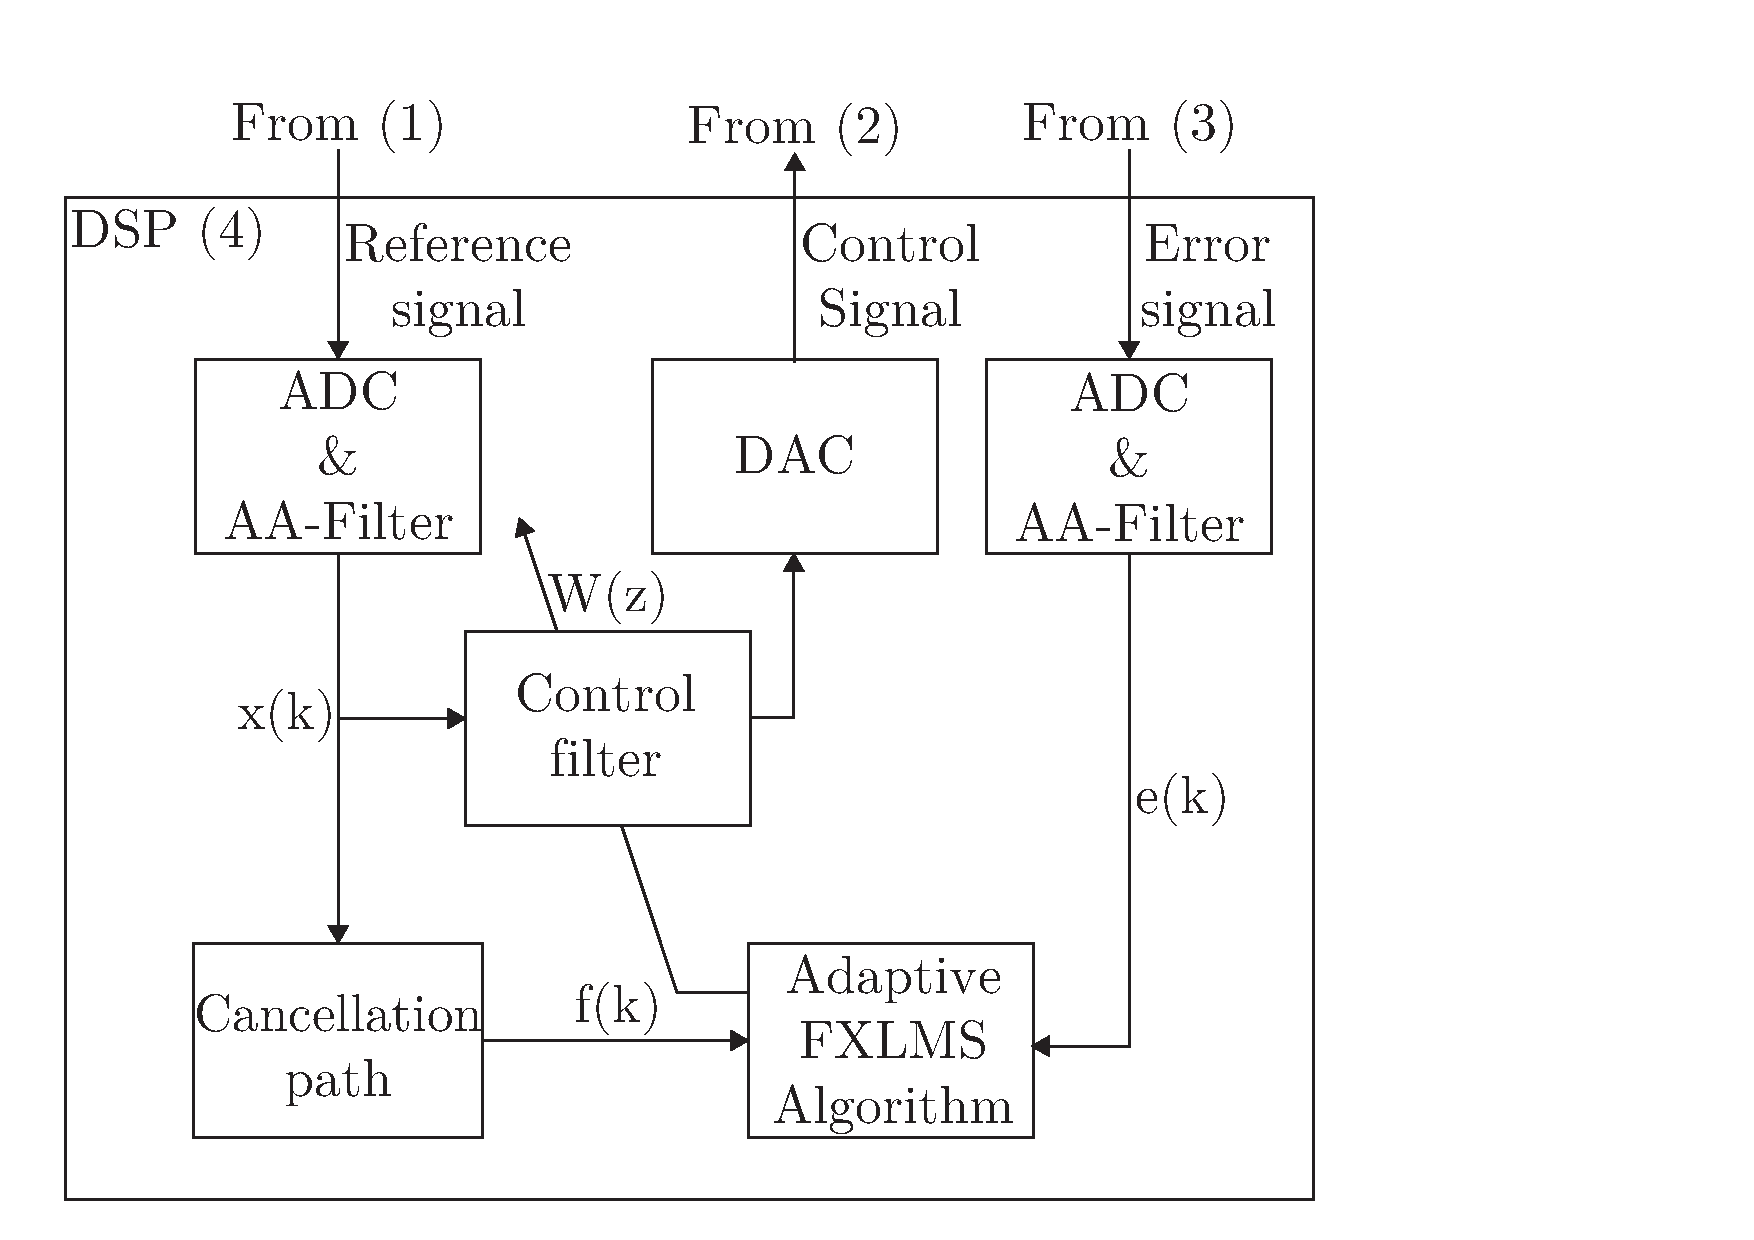
\includegraphics[width=1\columnwidth]{figures/ArticleIllustrations/ANCFeedForward}
		\tikzsetnextfilename{ANCFeedForward}
		\resizebox{0.95\columnwidth}{!}{
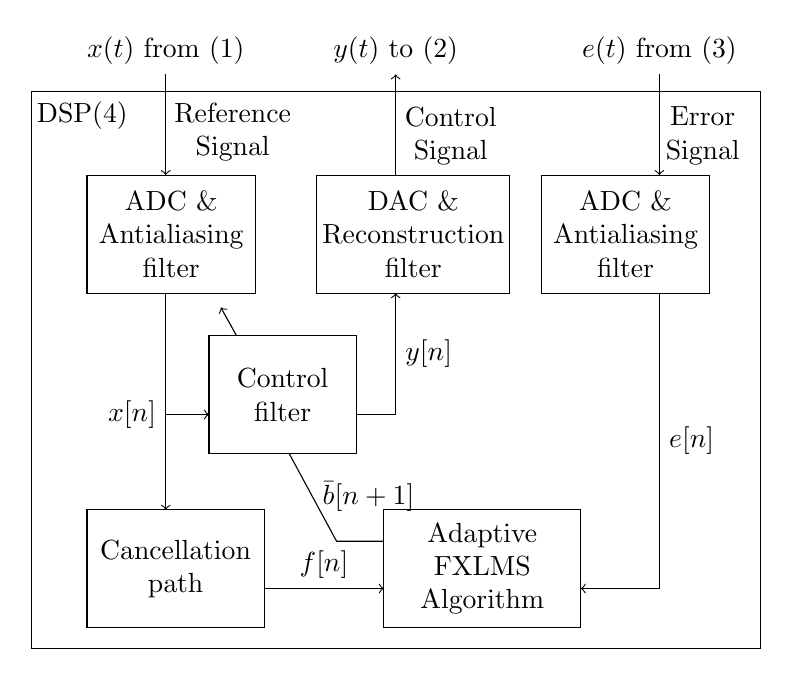
\begin{tikzpicture}
\draw  (-3,4.93) rectangle node[text width=2cm,align=center] {ADC \& Antialiasing filter} (-0.86,3.43);
\draw  (-3,0.68) rectangle node[text width=2.5cm,align=center] {Cancellation \\ path}(-0.75,-0.82);
\draw  (0.77,0.68) rectangle node[text width=2.5cm,align=center] {Adaptive FXLMS Algorithm} (3.27,-0.82);

\draw  (-1.45,2.89) rectangle node[text width=1.5cm,align=center,fill=white] {Control filter} (0.42,1.39);
\draw  (-0.08,4.93) rectangle node[text width=2.5cm,align=center] {DAC \& \\ Reconstruction filter}(2.37,3.43);
\draw  (2.77,4.93) rectangle node[text width=2cm,align=center] {ADC \& Antialiasing filter}(4.91,3.43);

\draw  (-3.71,5.99) rectangle (5.55,-1.08);
\node at (-3.06,5.69) {DSP(4)};
\node [text width=2cm,align=center] at (-1.15,5.48) {Reference Signal};

\draw[->] (-0.75,-0.32) -- node[above]{$f[n]$} (0.77,-0.32);

\draw[->] (4.27,3.43) -- node[right]{$e[n]$} (4.27,-0.32)  -- (3.27,-0.32);

\draw [->](4.27,6.21) node[above]{$e(t)$ from (3)} -- (4.27,4.93) ;
\draw [->](0.92,4.93)  --  (0.92,6.21) node[above]{$y(t)$ to (2)};
\draw [->](-2,3.43) -- (-2,0.68);

\draw [->](-2,1.89) node[left]{$x[n]$} -- (-1.45,1.89);

\draw[->] (0.42,1.89) -- (0.92,1.89) --node[right]{$y[n]$} (0.92,3.43);
\draw [->](-2,6.21) node[above]{$x(t)$ from (1)} -- (-2,4.93);
\node [text width=2cm,align=center] at (1.62,5.43) {Control Signal};
\node [text width=1.5cm,align=center] at (4.82,5.43) {Error Signal};

\draw (0.77,0.28) -- (0.17,0.28) --node[above=0.25,right]{$\bar{b}[n+1]$} (-0.43,1.39);
\draw [->](-1.1,2.89) -- (-1.3,3.25);
\end{tikzpicture}}
	\caption{Block diagram of adaptive feedforward ANC system. Expansion of DSP (4) from \autoref{fig:SystemOverview}.}
	\label{fig:ANCFeedforward}
\end{figure}

%The signals from (1) and (3) from \autoref{fig:ANCFeedforward} are converted to the digital domain using an ADC and anti-aliasing (AA) filters before processing. When processed, the output $y[n]$ is reconstructed using a DAC. \\\\

%\begin{figure}[H]
%	\centering
%	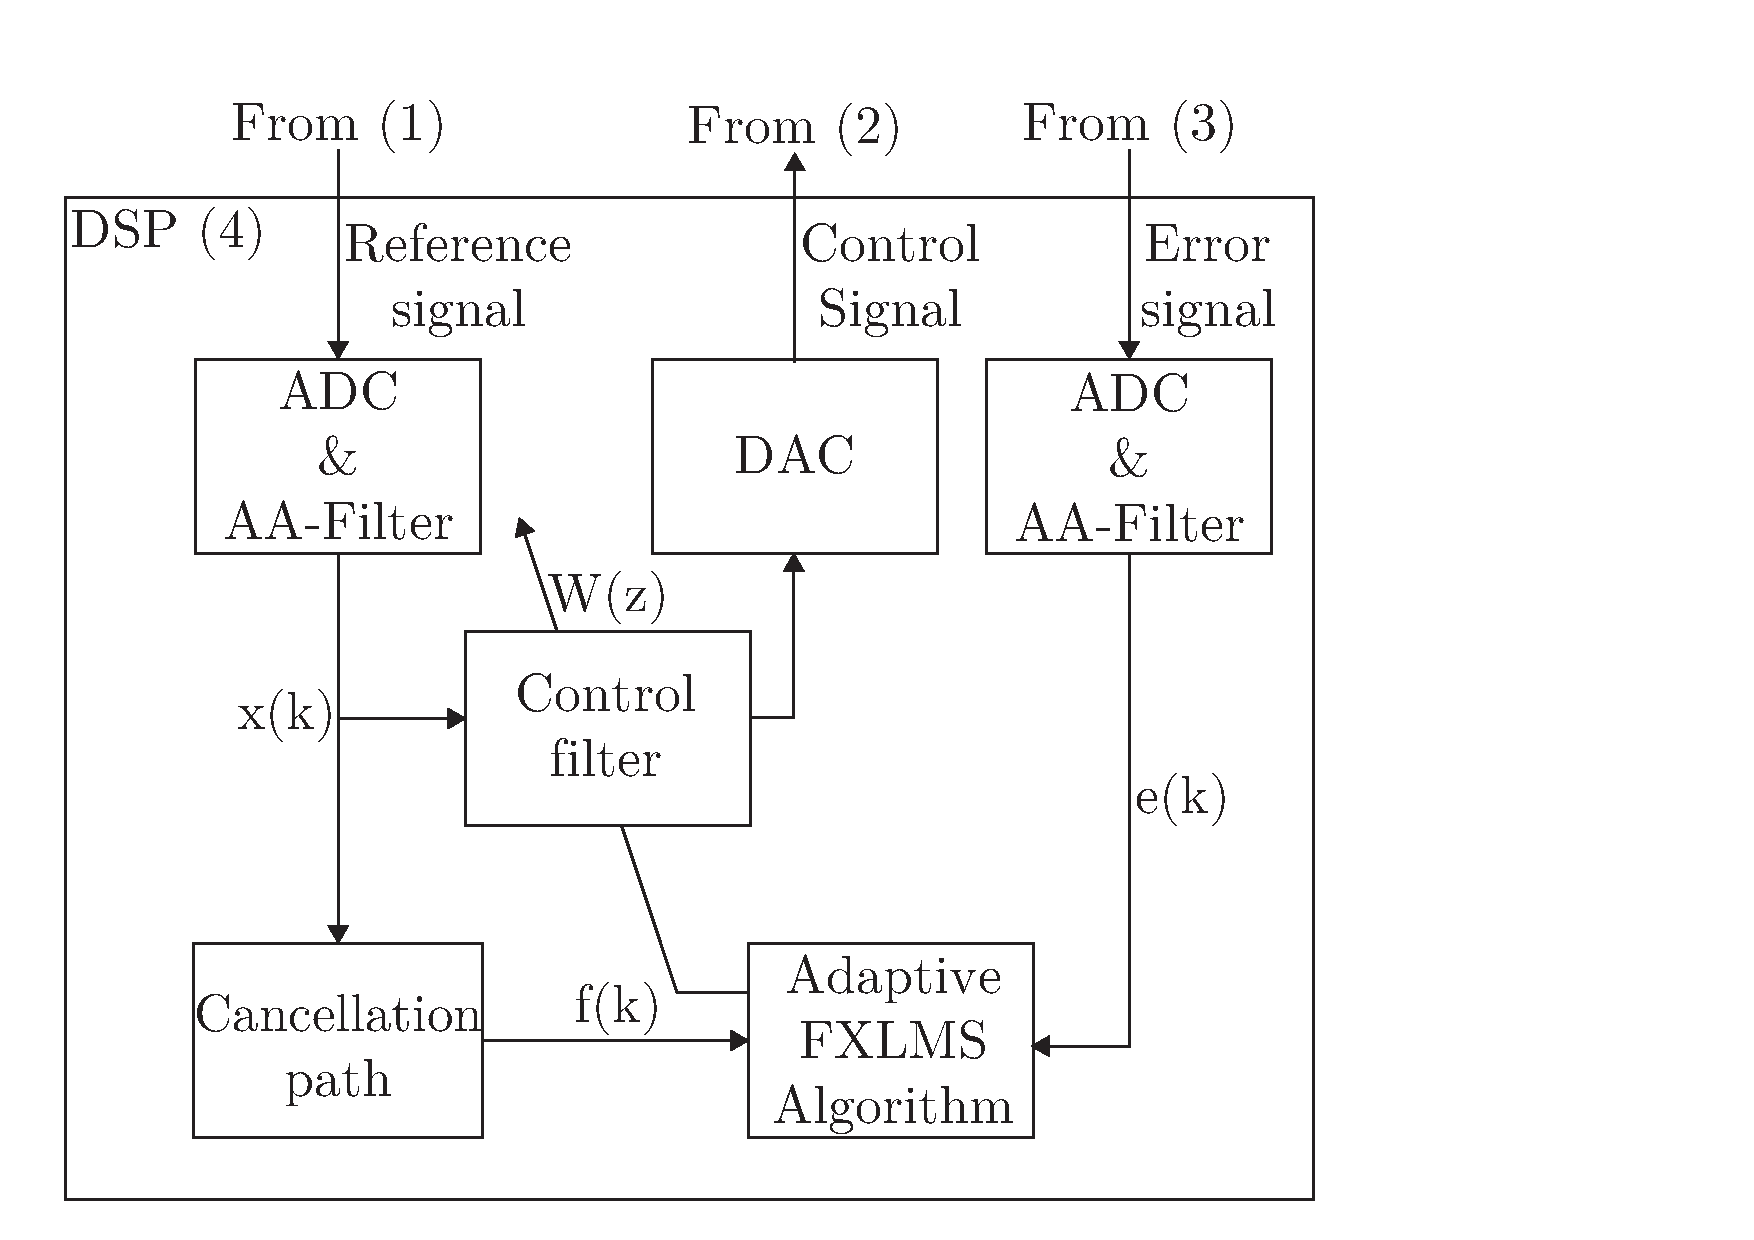
\includegraphics[width=1\columnwidth]{figures/ArticleIllustrations/ANCFeedForward}
%	\caption{Adaptive feedforward ANC system}
%	\label{fig:ANCFeedforward}
%\end{figure}

The Control Filter, shown in \autoref{eq:Output}, has an order of 960 taps to represent frequencies down to 50 Hz with $f_s = 48$ $k$Hz. 
%NO fucks given!
\begin{equation}\label{eq:Output}
y[n]=\sum_{j=0}^{L-1}b_j[n]x[n-j]
\end{equation}
Where: $b_j[n]$ are the weight coefficients written as  $b_j[n]=[b_0[n],b_1[n], \dotsc, b_{L-1}[n]]^T$. The control filter coefficients are updated using the FXLMS method shown in \autoref{eq:FXLMS}.
\begin{equation}\label{eq:FXLMS}
b_j[n+1] = b_j[n] - 2\mu e[n]f[n-j]
\end{equation}
Where: $\mu$ is the convergence factor, $e[n]$ is the error and $f[n]$ is the reference signal convolved with the Cancellation Path (CP) shown in \autoref{eq:CP}.
\begin{equation}\label{eq:CP}
f[n]=\sum_{j=0}^{L-1}c_jx[n-j]
\end{equation}
Where: $c_j$ is the coefficient of a measured transfer-function from the headphone loudspeaker to the error microphone in the ear of a Head and Torso Simulator (HATS). In the literature \cite{Hansen} the CP is adaptively adjusted, but it is assumed constant because the position of the headphone does not change while testing on a HATS. 


%When implementing the system, delays exist due to the anti-aliasing and reconstruction filters. The delays of the system exceeds the propagation time of sound from the reference microphone to the headphone loudspeaker resulting in poor performance. Therefore an LP-algorithm is proposed to predict future samples in order to decrease the effect of the time delays.
\subsection{Measuring HP and CP Transfer Functions}
The two transfer functions HP and CP were measured on a set of Beyerdynamic DT 770 Headphones in an anechoic chamber using a HATS. The setup is similar to \autoref{fig:SystemOverview} except the DSP (4) is replaced by a soundcard. When measuring HP a small microphone (spmMic) is placed by the headphone loudspeaker (2) and a loudspeaker is placed 1.6 m from the center of the HATS at 0\textdegree angle of incidence.  

\begin{figure}[H]
	\centering
	\tikzsetnextfilename{CancellationPathImpulseResponseCompareCP}
	%% This file was created by matlab2tikz.
%
%The latest updates can be retrieved from
%  http://www.mathworks.com/matlabcentral/fileexchange/22022-matlab2tikz-matlab2tikz
%where you can also make suggestions and rate matlab2tikz.
%
\definecolor{mycolor1}{rgb}{0.00000,0.44700,0.74100}%
\definecolor{mycolor2}{rgb}{0.85000,0.32500,0.09800}%
%
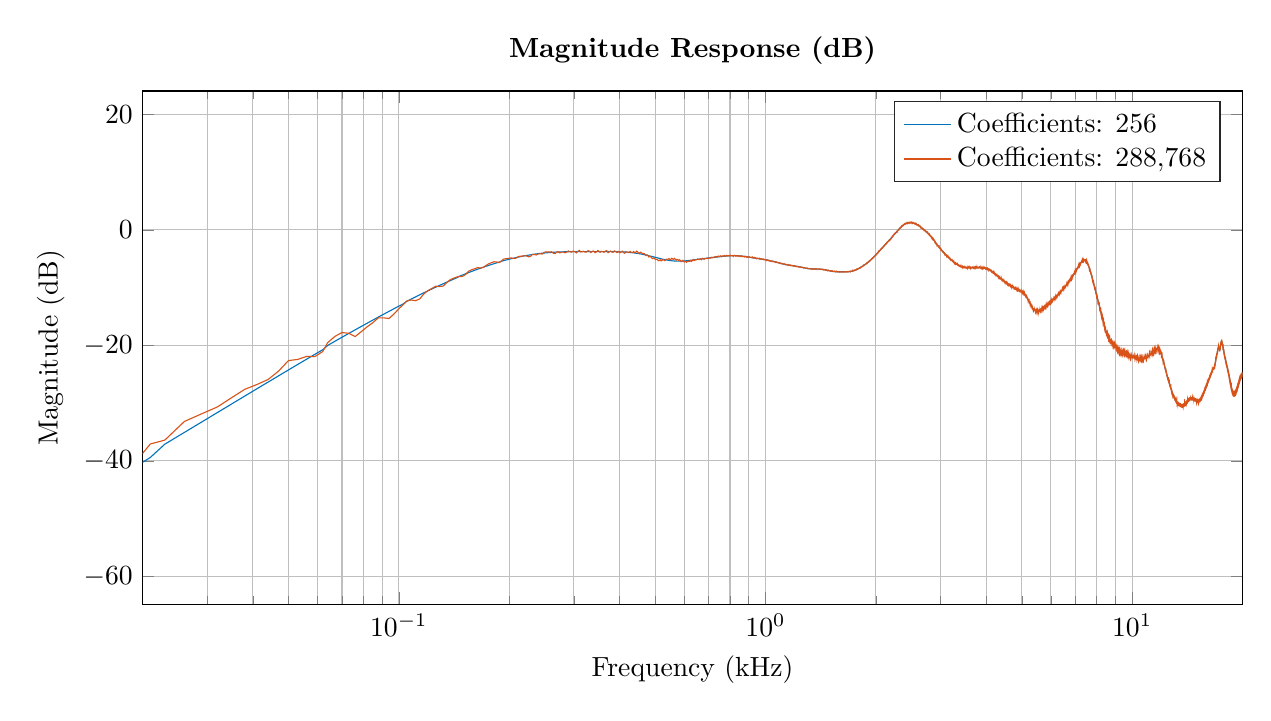
\begin{tikzpicture}

\begin{axis}[%
width=5.5in,
height=2.566in,
at={(2.804in,1.205in)},
scale only axis,
xmode=log,
xmin=0.020,
xmax=20.000,
xminorticks=true,
xlabel={Frequency (kHz)},
xmajorgrids,
xminorgrids,
ymin=-64.832,
ymax=24.080,
ylabel={Magnitude (dB)},
ymajorgrids,
axis background/.style={fill=white},
title style={font=\bfseries},
title={Magnitude Response (dB)},
legend style={legend cell align=left,align=left,draw=white!15!black}
]
\addplot [color=mycolor1,solid,forget plot]
  table[row sep=crcr]{%
0.018	-42.077\\
0.021	-39.419\\
0.023	-37.115\\
0.026	-35.084\\
0.029	-33.272\\
0.032	-31.636\\
0.035	-30.148\\
0.038	-28.784\\
0.041	-27.525\\
0.044	-26.358\\
0.047	-25.271\\
0.050	-24.254\\
0.053	-23.301\\
0.056	-22.403\\
0.059	-21.556\\
0.062	-20.755\\
0.064	-19.995\\
0.067	-19.274\\
0.070	-18.589\\
0.073	-17.935\\
0.076	-17.312\\
0.079	-16.718\\
0.082	-16.149\\
0.085	-15.605\\
0.088	-15.083\\
0.091	-14.584\\
0.094	-14.105\\
0.097	-13.645\\
0.100	-13.203\\
0.103	-12.779\\
0.105	-12.371\\
0.108	-11.979\\
0.111	-11.602\\
0.114	-11.239\\
0.117	-10.890\\
0.120	-10.554\\
0.123	-10.231\\
0.126	-9.920\\
0.129	-9.620\\
0.132	-9.332\\
0.135	-9.055\\
0.138	-8.788\\
0.141	-8.531\\
0.144	-8.284\\
0.146	-8.046\\
0.149	-7.818\\
0.152	-7.598\\
0.155	-7.387\\
0.158	-7.184\\
0.161	-6.990\\
0.164	-6.803\\
0.167	-6.624\\
0.170	-6.452\\
0.173	-6.288\\
0.176	-6.131\\
0.179	-5.980\\
0.182	-5.836\\
0.185	-5.699\\
0.188	-5.568\\
0.190	-5.443\\
0.193	-5.324\\
0.196	-5.211\\
0.199	-5.103\\
0.202	-5.001\\
0.205	-4.904\\
0.208	-4.813\\
0.211	-4.727\\
0.214	-4.645\\
0.217	-4.568\\
0.220	-4.496\\
0.223	-4.428\\
0.226	-4.365\\
0.229	-4.306\\
0.231	-4.251\\
0.234	-4.199\\
0.237	-4.152\\
0.240	-4.108\\
0.243	-4.068\\
0.246	-4.030\\
0.249	-3.996\\
0.252	-3.965\\
0.255	-3.937\\
0.258	-3.912\\
0.261	-3.889\\
0.264	-3.869\\
0.267	-3.850\\
0.270	-3.834\\
0.272	-3.820\\
0.275	-3.808\\
0.278	-3.798\\
0.281	-3.789\\
0.284	-3.781\\
0.287	-3.775\\
0.290	-3.770\\
0.293	-3.766\\
0.296	-3.763\\
0.299	-3.760\\
0.302	-3.759\\
0.305	-3.758\\
0.308	-3.757\\
0.311	-3.757\\
0.313	-3.757\\
0.316	-3.757\\
0.319	-3.757\\
0.322	-3.757\\
0.325	-3.758\\
0.328	-3.758\\
0.331	-3.758\\
0.334	-3.758\\
0.337	-3.759\\
0.340	-3.758\\
0.343	-3.758\\
0.346	-3.758\\
0.349	-3.758\\
0.352	-3.757\\
0.354	-3.757\\
0.357	-3.756\\
0.360	-3.756\\
0.363	-3.755\\
0.366	-3.755\\
0.369	-3.755\\
0.372	-3.755\\
0.375	-3.756\\
0.378	-3.757\\
0.381	-3.758\\
0.384	-3.760\\
0.387	-3.763\\
0.390	-3.767\\
0.393	-3.771\\
0.396	-3.776\\
0.398	-3.782\\
0.401	-3.789\\
0.404	-3.797\\
0.407	-3.806\\
0.410	-3.816\\
0.413	-3.827\\
0.416	-3.840\\
0.419	-3.854\\
0.422	-3.870\\
0.425	-3.886\\
0.428	-3.905\\
0.431	-3.924\\
0.434	-3.945\\
0.437	-3.968\\
0.439	-3.992\\
0.442	-4.017\\
0.445	-4.044\\
0.448	-4.072\\
0.451	-4.102\\
0.454	-4.133\\
0.457	-4.165\\
0.460	-4.198\\
0.463	-4.233\\
0.466	-4.269\\
0.469	-4.305\\
0.472	-4.343\\
0.475	-4.382\\
0.478	-4.421\\
0.480	-4.461\\
0.483	-4.502\\
0.486	-4.543\\
0.489	-4.585\\
0.492	-4.627\\
0.495	-4.668\\
0.498	-4.710\\
0.501	-4.752\\
0.504	-4.793\\
0.507	-4.834\\
0.510	-4.874\\
0.513	-4.914\\
0.516	-4.953\\
0.519	-4.991\\
0.521	-5.028\\
0.524	-5.063\\
0.527	-5.097\\
0.530	-5.130\\
0.533	-5.161\\
0.536	-5.191\\
0.539	-5.219\\
0.542	-5.245\\
0.545	-5.269\\
0.548	-5.291\\
0.551	-5.312\\
0.554	-5.330\\
0.557	-5.346\\
0.560	-5.361\\
0.562	-5.373\\
0.565	-5.383\\
0.568	-5.391\\
0.571	-5.398\\
0.574	-5.402\\
0.577	-5.405\\
0.580	-5.405\\
0.583	-5.405\\
0.586	-5.402\\
0.589	-5.398\\
0.592	-5.392\\
0.595	-5.386\\
0.598	-5.377\\
0.601	-5.368\\
0.604	-5.358\\
0.606	-5.346\\
0.609	-5.334\\
0.612	-5.321\\
0.615	-5.307\\
0.618	-5.293\\
0.621	-5.278\\
0.624	-5.263\\
0.627	-5.247\\
0.630	-5.231\\
0.633	-5.215\\
0.636	-5.199\\
0.639	-5.182\\
0.642	-5.166\\
0.645	-5.149\\
0.647	-5.133\\
0.650	-5.116\\
0.653	-5.100\\
0.656	-5.084\\
0.659	-5.068\\
0.662	-5.052\\
0.665	-5.036\\
0.668	-5.021\\
0.671	-5.005\\
0.674	-4.990\\
0.677	-4.975\\
0.680	-4.960\\
0.683	-4.946\\
0.686	-4.931\\
0.688	-4.917\\
0.691	-4.902\\
0.694	-4.888\\
0.697	-4.874\\
0.700	-4.860\\
0.703	-4.847\\
0.706	-4.833\\
0.709	-4.819\\
0.712	-4.806\\
0.715	-4.792\\
0.718	-4.778\\
0.721	-4.765\\
0.724	-4.751\\
0.727	-4.738\\
0.729	-4.725\\
0.732	-4.711\\
0.735	-4.698\\
0.738	-4.685\\
0.741	-4.672\\
0.744	-4.659\\
0.747	-4.646\\
0.750	-4.633\\
0.753	-4.621\\
0.756	-4.608\\
0.759	-4.596\\
0.762	-4.584\\
0.765	-4.573\\
0.768	-4.561\\
0.771	-4.550\\
0.773	-4.540\\
0.776	-4.530\\
0.779	-4.520\\
0.782	-4.511\\
0.785	-4.502\\
0.788	-4.494\\
0.791	-4.487\\
0.794	-4.480\\
0.797	-4.473\\
0.800	-4.468\\
0.803	-4.463\\
0.806	-4.458\\
0.809	-4.455\\
0.812	-4.452\\
0.814	-4.450\\
0.817	-4.449\\
0.820	-4.449\\
0.823	-4.449\\
0.826	-4.450\\
0.829	-4.452\\
0.832	-4.455\\
0.835	-4.459\\
0.838	-4.463\\
0.841	-4.469\\
0.844	-4.475\\
0.847	-4.481\\
0.850	-4.489\\
0.853	-4.497\\
0.855	-4.506\\
0.858	-4.516\\
0.861	-4.526\\
0.864	-4.537\\
0.867	-4.548\\
0.870	-4.560\\
0.873	-4.573\\
0.876	-4.586\\
0.879	-4.599\\
0.882	-4.613\\
0.885	-4.627\\
0.888	-4.641\\
0.891	-4.656\\
0.894	-4.671\\
0.896	-4.686\\
0.899	-4.701\\
0.902	-4.716\\
0.905	-4.732\\
0.908	-4.747\\
0.911	-4.762\\
0.914	-4.778\\
0.917	-4.793\\
0.920	-4.808\\
0.923	-4.823\\
0.926	-4.838\\
0.929	-4.852\\
0.932	-4.867\\
0.935	-4.881\\
0.938	-4.895\\
0.940	-4.909\\
0.943	-4.923\\
0.946	-4.937\\
0.949	-4.950\\
0.952	-4.963\\
0.955	-4.976\\
0.958	-4.989\\
0.961	-5.001\\
0.964	-5.014\\
0.967	-5.026\\
0.970	-5.039\\
0.973	-5.051\\
0.976	-5.063\\
0.979	-5.075\\
0.981	-5.088\\
0.984	-5.100\\
0.987	-5.112\\
0.990	-5.125\\
0.993	-5.138\\
0.996	-5.150\\
0.999	-5.164\\
1.002	-5.177\\
1.005	-5.190\\
1.008	-5.204\\
1.011	-5.219\\
1.014	-5.233\\
1.017	-5.248\\
1.020	-5.263\\
1.022	-5.279\\
1.025	-5.295\\
1.028	-5.311\\
1.031	-5.328\\
1.034	-5.345\\
1.037	-5.362\\
1.040	-5.380\\
1.043	-5.398\\
1.046	-5.417\\
1.049	-5.436\\
1.052	-5.455\\
1.055	-5.475\\
1.058	-5.494\\
1.061	-5.515\\
1.063	-5.535\\
1.066	-5.555\\
1.069	-5.576\\
1.072	-5.597\\
1.075	-5.618\\
1.078	-5.638\\
1.081	-5.659\\
1.084	-5.680\\
1.087	-5.701\\
1.090	-5.721\\
1.093	-5.742\\
1.096	-5.762\\
1.099	-5.782\\
1.102	-5.802\\
1.104	-5.821\\
1.107	-5.841\\
1.110	-5.859\\
1.113	-5.878\\
1.116	-5.896\\
1.119	-5.913\\
1.122	-5.930\\
1.125	-5.947\\
1.128	-5.963\\
1.131	-5.978\\
1.134	-5.994\\
1.137	-6.008\\
1.140	-6.022\\
1.143	-6.036\\
1.146	-6.049\\
1.148	-6.062\\
1.151	-6.074\\
1.154	-6.086\\
1.157	-6.098\\
1.160	-6.109\\
1.163	-6.120\\
1.166	-6.130\\
1.169	-6.140\\
1.172	-6.150\\
1.175	-6.160\\
1.178	-6.170\\
1.181	-6.179\\
1.184	-6.189\\
1.187	-6.198\\
1.189	-6.208\\
1.192	-6.217\\
1.195	-6.227\\
1.198	-6.236\\
1.201	-6.246\\
1.204	-6.256\\
1.207	-6.266\\
1.210	-6.276\\
1.213	-6.287\\
1.216	-6.298\\
1.219	-6.309\\
1.222	-6.320\\
1.225	-6.331\\
1.228	-6.343\\
1.230	-6.355\\
1.233	-6.368\\
1.236	-6.380\\
1.239	-6.393\\
1.242	-6.406\\
1.245	-6.420\\
1.248	-6.433\\
1.251	-6.447\\
1.254	-6.461\\
1.257	-6.475\\
1.260	-6.489\\
1.263	-6.503\\
1.266	-6.517\\
1.269	-6.531\\
1.271	-6.545\\
1.274	-6.559\\
1.277	-6.573\\
1.280	-6.587\\
1.283	-6.600\\
1.286	-6.613\\
1.289	-6.626\\
1.292	-6.638\\
1.295	-6.650\\
1.298	-6.661\\
1.301	-6.672\\
1.304	-6.683\\
1.307	-6.693\\
1.310	-6.702\\
1.312	-6.711\\
1.315	-6.720\\
1.318	-6.727\\
1.321	-6.734\\
1.324	-6.741\\
1.327	-6.747\\
1.330	-6.752\\
1.333	-6.757\\
1.336	-6.761\\
1.339	-6.765\\
1.342	-6.768\\
1.345	-6.770\\
1.348	-6.772\\
1.351	-6.774\\
1.354	-6.775\\
1.356	-6.776\\
1.359	-6.777\\
1.362	-6.777\\
1.365	-6.777\\
1.368	-6.777\\
1.371	-6.777\\
1.374	-6.777\\
1.377	-6.777\\
1.380	-6.777\\
1.383	-6.777\\
1.386	-6.777\\
1.389	-6.777\\
1.392	-6.778\\
1.395	-6.778\\
1.397	-6.780\\
1.400	-6.781\\
1.403	-6.783\\
1.406	-6.785\\
1.409	-6.788\\
1.412	-6.791\\
1.415	-6.795\\
1.418	-6.800\\
1.421	-6.804\\
1.424	-6.810\\
1.427	-6.816\\
1.430	-6.823\\
1.433	-6.830\\
1.436	-6.837\\
1.438	-6.846\\
1.441	-6.855\\
1.444	-6.864\\
1.447	-6.874\\
1.450	-6.884\\
1.453	-6.895\\
1.456	-6.906\\
1.459	-6.918\\
1.462	-6.930\\
1.465	-6.942\\
1.468	-6.955\\
1.471	-6.967\\
1.474	-6.980\\
1.477	-6.993\\
1.479	-7.006\\
1.482	-7.020\\
1.485	-7.033\\
1.488	-7.046\\
1.491	-7.059\\
1.494	-7.071\\
1.497	-7.084\\
1.500	-7.096\\
1.503	-7.108\\
1.506	-7.120\\
1.509	-7.131\\
1.512	-7.142\\
1.515	-7.153\\
1.518	-7.162\\
1.521	-7.172\\
1.523	-7.181\\
1.526	-7.189\\
1.529	-7.197\\
1.532	-7.204\\
1.535	-7.211\\
1.538	-7.217\\
1.541	-7.222\\
1.544	-7.227\\
1.547	-7.232\\
1.550	-7.236\\
1.553	-7.239\\
1.556	-7.242\\
1.559	-7.244\\
1.562	-7.246\\
1.564	-7.248\\
1.567	-7.249\\
1.570	-7.250\\
1.573	-7.251\\
1.576	-7.251\\
1.579	-7.251\\
1.582	-7.251\\
1.585	-7.250\\
1.588	-7.250\\
1.591	-7.249\\
1.594	-7.248\\
1.597	-7.247\\
1.600	-7.247\\
1.603	-7.246\\
1.605	-7.245\\
1.608	-7.244\\
1.611	-7.244\\
1.614	-7.243\\
1.617	-7.243\\
1.620	-7.242\\
1.623	-7.242\\
1.626	-7.242\\
1.629	-7.242\\
1.632	-7.242\\
1.635	-7.242\\
1.638	-7.242\\
1.641	-7.243\\
1.644	-7.243\\
1.646	-7.243\\
1.649	-7.244\\
1.652	-7.244\\
1.655	-7.244\\
1.658	-7.245\\
1.661	-7.245\\
1.664	-7.245\\
1.667	-7.244\\
1.670	-7.244\\
1.673	-7.243\\
1.676	-7.242\\
1.679	-7.240\\
1.682	-7.238\\
1.685	-7.236\\
1.688	-7.233\\
1.690	-7.230\\
1.693	-7.226\\
1.696	-7.221\\
1.699	-7.216\\
1.702	-7.210\\
1.705	-7.204\\
1.708	-7.196\\
1.711	-7.188\\
1.714	-7.180\\
1.717	-7.170\\
1.720	-7.160\\
1.723	-7.149\\
1.726	-7.137\\
1.729	-7.125\\
1.731	-7.111\\
1.734	-7.097\\
1.737	-7.082\\
1.740	-7.067\\
1.743	-7.050\\
1.746	-7.033\\
1.749	-7.016\\
1.752	-6.997\\
1.755	-6.978\\
1.758	-6.959\\
1.761	-6.938\\
1.764	-6.917\\
1.767	-6.896\\
1.770	-6.874\\
1.772	-6.852\\
1.775	-6.829\\
1.778	-6.806\\
1.781	-6.783\\
1.784	-6.759\\
1.787	-6.735\\
1.790	-6.711\\
1.793	-6.686\\
1.796	-6.661\\
1.799	-6.636\\
1.802	-6.611\\
1.805	-6.586\\
1.808	-6.560\\
1.811	-6.534\\
1.813	-6.509\\
1.816	-6.483\\
1.819	-6.457\\
1.822	-6.431\\
1.825	-6.404\\
1.828	-6.378\\
1.831	-6.352\\
1.834	-6.325\\
1.837	-6.298\\
1.840	-6.271\\
1.843	-6.244\\
1.846	-6.217\\
1.849	-6.190\\
1.852	-6.162\\
1.854	-6.135\\
1.857	-6.107\\
1.860	-6.078\\
1.863	-6.050\\
1.866	-6.021\\
1.869	-5.992\\
1.872	-5.963\\
1.875	-5.933\\
1.878	-5.903\\
1.881	-5.872\\
1.884	-5.841\\
1.887	-5.810\\
1.890	-5.778\\
1.893	-5.746\\
1.896	-5.713\\
1.898	-5.680\\
1.901	-5.647\\
1.904	-5.613\\
1.907	-5.578\\
1.910	-5.543\\
1.913	-5.508\\
1.916	-5.472\\
1.919	-5.435\\
1.922	-5.398\\
1.925	-5.361\\
1.928	-5.323\\
1.931	-5.285\\
1.934	-5.246\\
1.937	-5.207\\
1.939	-5.168\\
1.942	-5.128\\
1.945	-5.088\\
1.948	-5.047\\
1.951	-5.006\\
1.954	-4.965\\
1.957	-4.924\\
1.960	-4.882\\
1.963	-4.840\\
1.966	-4.798\\
1.969	-4.755\\
1.972	-4.713\\
1.975	-4.670\\
1.978	-4.627\\
1.980	-4.584\\
1.983	-4.541\\
1.986	-4.498\\
1.989	-4.455\\
1.992	-4.411\\
1.995	-4.368\\
1.998	-4.325\\
2.001	-4.281\\
2.004	-4.238\\
2.007	-4.195\\
2.010	-4.151\\
2.013	-4.108\\
2.016	-4.065\\
2.019	-4.021\\
2.021	-3.978\\
2.024	-3.935\\
2.027	-3.892\\
2.030	-3.849\\
2.033	-3.807\\
2.036	-3.764\\
2.039	-3.721\\
2.042	-3.678\\
2.045	-3.636\\
2.048	-3.593\\
2.051	-3.551\\
2.054	-3.509\\
2.057	-3.466\\
2.060	-3.424\\
2.062	-3.382\\
2.065	-3.340\\
2.068	-3.298\\
2.071	-3.256\\
2.074	-3.214\\
2.077	-3.172\\
2.080	-3.130\\
2.083	-3.088\\
2.086	-3.047\\
2.089	-3.005\\
2.092	-2.963\\
2.095	-2.921\\
2.098	-2.880\\
2.101	-2.838\\
2.104	-2.796\\
2.106	-2.755\\
2.109	-2.713\\
2.112	-2.672\\
2.115	-2.630\\
2.118	-2.588\\
2.121	-2.547\\
2.124	-2.505\\
2.127	-2.464\\
2.130	-2.422\\
2.133	-2.381\\
2.136	-2.339\\
2.139	-2.298\\
2.142	-2.256\\
2.145	-2.215\\
2.147	-2.174\\
2.150	-2.132\\
2.153	-2.091\\
2.156	-2.049\\
2.159	-2.008\\
2.162	-1.967\\
2.165	-1.925\\
2.168	-1.884\\
2.171	-1.843\\
2.174	-1.801\\
2.177	-1.760\\
2.180	-1.718\\
2.183	-1.677\\
2.186	-1.636\\
2.188	-1.594\\
2.191	-1.553\\
2.194	-1.512\\
2.197	-1.470\\
2.200	-1.429\\
2.203	-1.388\\
2.206	-1.346\\
2.209	-1.305\\
2.212	-1.263\\
2.215	-1.222\\
2.218	-1.181\\
2.221	-1.139\\
2.224	-1.098\\
2.227	-1.056\\
2.229	-1.015\\
2.232	-0.973\\
2.235	-0.932\\
2.238	-0.890\\
2.241	-0.848\\
2.244	-0.807\\
2.247	-0.765\\
2.250	-0.724\\
2.253	-0.682\\
2.256	-0.641\\
2.259	-0.599\\
2.262	-0.558\\
2.265	-0.517\\
2.268	-0.476\\
2.271	-0.434\\
2.273	-0.393\\
2.276	-0.352\\
2.279	-0.312\\
2.282	-0.271\\
2.285	-0.230\\
2.288	-0.190\\
2.291	-0.150\\
2.294	-0.110\\
2.297	-0.070\\
2.300	-0.031\\
2.303	0.009\\
2.306	0.047\\
2.309	0.086\\
2.312	0.124\\
2.314	0.162\\
2.317	0.200\\
2.320	0.237\\
2.323	0.274\\
2.326	0.310\\
2.329	0.346\\
2.332	0.381\\
2.335	0.416\\
2.338	0.450\\
2.341	0.484\\
2.344	0.517\\
2.347	0.550\\
2.350	0.582\\
2.353	0.613\\
2.355	0.644\\
2.358	0.674\\
2.361	0.704\\
2.364	0.733\\
2.367	0.761\\
2.370	0.788\\
2.373	0.815\\
2.376	0.841\\
2.379	0.867\\
2.382	0.891\\
2.385	0.915\\
2.388	0.938\\
2.391	0.960\\
2.394	0.982\\
2.396	1.002\\
2.399	1.022\\
2.402	1.042\\
2.405	1.060\\
2.408	1.077\\
2.411	1.094\\
2.414	1.110\\
2.417	1.126\\
2.420	1.140\\
2.423	1.154\\
2.426	1.167\\
2.429	1.179\\
2.432	1.190\\
2.435	1.201\\
2.438	1.211\\
2.440	1.220\\
2.443	1.228\\
2.446	1.236\\
2.449	1.243\\
2.452	1.249\\
2.455	1.255\\
2.458	1.260\\
2.461	1.264\\
2.464	1.268\\
2.467	1.270\\
2.470	1.273\\
2.473	1.274\\
2.476	1.275\\
2.479	1.276\\
2.481	1.275\\
2.484	1.275\\
2.487	1.273\\
2.490	1.271\\
2.493	1.269\\
2.496	1.266\\
2.499	1.262\\
2.502	1.258\\
2.505	1.253\\
2.508	1.248\\
2.511	1.242\\
2.514	1.236\\
2.517	1.229\\
2.520	1.222\\
2.522	1.214\\
2.525	1.206\\
2.528	1.198\\
2.531	1.189\\
2.534	1.179\\
2.537	1.169\\
2.540	1.159\\
2.543	1.148\\
2.546	1.136\\
2.549	1.125\\
2.552	1.113\\
2.555	1.100\\
2.558	1.087\\
2.561	1.074\\
2.563	1.060\\
2.566	1.046\\
2.569	1.031\\
2.572	1.016\\
2.575	1.001\\
2.578	0.985\\
2.581	0.969\\
2.584	0.952\\
2.587	0.936\\
2.590	0.918\\
2.593	0.901\\
2.596	0.883\\
2.599	0.864\\
2.602	0.846\\
2.604	0.827\\
2.607	0.807\\
2.610	0.788\\
2.613	0.768\\
2.616	0.747\\
2.619	0.727\\
2.622	0.706\\
2.625	0.685\\
2.628	0.663\\
2.631	0.641\\
2.634	0.620\\
2.637	0.597\\
2.640	0.575\\
2.643	0.552\\
2.646	0.529\\
2.648	0.506\\
2.651	0.483\\
2.654	0.459\\
2.657	0.436\\
2.660	0.412\\
2.663	0.388\\
2.666	0.364\\
2.669	0.340\\
2.672	0.315\\
2.675	0.291\\
2.678	0.266\\
2.681	0.242\\
2.684	0.217\\
2.687	0.192\\
2.689	0.167\\
2.692	0.142\\
2.695	0.117\\
2.698	0.092\\
2.701	0.067\\
2.704	0.041\\
2.707	0.016\\
2.710	-0.009\\
2.713	-0.035\\
2.716	-0.060\\
2.719	-0.086\\
2.722	-0.111\\
2.725	-0.137\\
2.728	-0.163\\
2.730	-0.189\\
2.733	-0.214\\
2.736	-0.240\\
2.739	-0.266\\
2.742	-0.293\\
2.745	-0.319\\
2.748	-0.345\\
2.751	-0.372\\
2.754	-0.398\\
2.757	-0.425\\
2.760	-0.452\\
2.763	-0.479\\
2.766	-0.507\\
2.769	-0.534\\
2.771	-0.562\\
2.774	-0.590\\
2.777	-0.618\\
2.780	-0.647\\
2.783	-0.675\\
2.786	-0.704\\
2.789	-0.734\\
2.792	-0.763\\
2.795	-0.793\\
2.798	-0.823\\
2.801	-0.854\\
2.804	-0.884\\
2.807	-0.916\\
2.810	-0.947\\
2.812	-0.979\\
2.815	-1.011\\
2.818	-1.043\\
2.821	-1.076\\
2.824	-1.109\\
2.827	-1.143\\
2.830	-1.177\\
2.833	-1.211\\
2.836	-1.245\\
2.839	-1.280\\
2.842	-1.315\\
2.845	-1.351\\
2.848	-1.387\\
2.851	-1.423\\
2.854	-1.459\\
2.856	-1.496\\
2.859	-1.533\\
2.862	-1.570\\
2.865	-1.607\\
2.868	-1.644\\
2.871	-1.682\\
2.874	-1.720\\
2.877	-1.758\\
2.880	-1.796\\
2.883	-1.835\\
2.886	-1.873\\
2.889	-1.911\\
2.892	-1.950\\
2.895	-1.989\\
2.897	-2.027\\
2.900	-2.066\\
2.903	-2.104\\
2.906	-2.143\\
2.909	-2.181\\
2.912	-2.220\\
2.915	-2.258\\
2.918	-2.296\\
2.921	-2.334\\
2.924	-2.372\\
2.927	-2.410\\
2.930	-2.447\\
2.933	-2.485\\
2.936	-2.522\\
2.938	-2.559\\
2.941	-2.595\\
2.944	-2.632\\
2.947	-2.668\\
2.950	-2.704\\
2.953	-2.740\\
2.956	-2.776\\
2.959	-2.811\\
2.962	-2.846\\
2.965	-2.881\\
2.968	-2.915\\
2.971	-2.950\\
2.974	-2.984\\
2.977	-3.018\\
2.979	-3.051\\
2.982	-3.085\\
2.985	-3.118\\
2.988	-3.151\\
2.991	-3.184\\
2.994	-3.216\\
2.997	-3.248\\
3.000	-3.281\\
3.003	-3.313\\
3.006	-3.344\\
3.009	-3.376\\
3.012	-3.407\\
3.015	-3.439\\
3.018	-3.470\\
3.021	-3.501\\
3.023	-3.531\\
3.026	-3.562\\
3.029	-3.593\\
3.032	-3.623\\
3.035	-3.653\\
3.038	-3.684\\
3.041	-3.714\\
3.044	-3.744\\
3.047	-3.773\\
3.050	-3.803\\
3.053	-3.833\\
3.056	-3.862\\
3.059	-3.891\\
3.062	-3.921\\
3.064	-3.950\\
3.067	-3.979\\
3.070	-4.007\\
3.073	-4.036\\
3.076	-4.064\\
3.079	-4.093\\
3.082	-4.121\\
3.085	-4.149\\
3.088	-4.177\\
3.091	-4.204\\
3.094	-4.232\\
3.097	-4.259\\
3.100	-4.286\\
3.103	-4.313\\
3.105	-4.340\\
3.108	-4.366\\
3.111	-4.392\\
3.114	-4.418\\
3.117	-4.444\\
3.120	-4.470\\
3.123	-4.495\\
3.126	-4.521\\
3.129	-4.546\\
3.132	-4.570\\
3.135	-4.595\\
3.138	-4.619\\
3.141	-4.644\\
3.144	-4.668\\
3.146	-4.691\\
3.149	-4.715\\
3.152	-4.739\\
3.155	-4.762\\
3.158	-4.785\\
3.161	-4.808\\
3.164	-4.831\\
3.167	-4.853\\
3.170	-4.876\\
3.173	-4.898\\
3.176	-4.921\\
3.179	-4.943\\
3.182	-4.965\\
3.185	-4.987\\
3.188	-5.009\\
3.190	-5.030\\
3.193	-5.052\\
3.196	-5.074\\
3.199	-5.096\\
3.202	-5.117\\
3.205	-5.139\\
3.208	-5.160\\
3.211	-5.182\\
3.214	-5.203\\
3.217	-5.224\\
3.220	-5.246\\
3.223	-5.267\\
3.226	-5.288\\
3.229	-5.309\\
3.231	-5.330\\
3.234	-5.352\\
3.237	-5.373\\
3.240	-5.394\\
3.243	-5.415\\
3.246	-5.435\\
3.249	-5.456\\
3.252	-5.477\\
3.255	-5.497\\
3.258	-5.518\\
3.261	-5.538\\
3.264	-5.558\\
3.267	-5.579\\
3.270	-5.599\\
3.272	-5.618\\
3.275	-5.638\\
3.278	-5.657\\
3.281	-5.677\\
3.284	-5.696\\
3.287	-5.715\\
3.290	-5.733\\
3.293	-5.752\\
3.296	-5.770\\
3.299	-5.788\\
3.302	-5.805\\
3.305	-5.823\\
3.308	-5.840\\
3.311	-5.857\\
3.313	-5.873\\
3.316	-5.890\\
3.319	-5.906\\
3.322	-5.921\\
3.325	-5.937\\
3.328	-5.952\\
3.331	-5.967\\
3.334	-5.982\\
3.337	-5.996\\
3.340	-6.010\\
3.343	-6.024\\
3.346	-6.038\\
3.349	-6.051\\
3.352	-6.064\\
3.354	-6.077\\
3.357	-6.090\\
3.360	-6.102\\
3.363	-6.114\\
3.366	-6.126\\
3.369	-6.138\\
3.372	-6.149\\
3.375	-6.161\\
3.378	-6.172\\
3.381	-6.183\\
3.384	-6.194\\
3.387	-6.205\\
3.390	-6.215\\
3.393	-6.225\\
3.396	-6.236\\
3.398	-6.246\\
3.401	-6.256\\
3.404	-6.266\\
3.407	-6.275\\
3.410	-6.285\\
3.413	-6.295\\
3.416	-6.304\\
3.419	-6.313\\
3.422	-6.322\\
3.425	-6.331\\
3.428	-6.340\\
3.431	-6.349\\
3.434	-6.357\\
3.437	-6.365\\
3.439	-6.374\\
3.442	-6.382\\
3.445	-6.390\\
3.448	-6.397\\
3.451	-6.405\\
3.454	-6.412\\
3.457	-6.419\\
3.460	-6.426\\
3.463	-6.433\\
3.466	-6.440\\
3.469	-6.446\\
3.472	-6.452\\
3.475	-6.458\\
3.478	-6.463\\
3.480	-6.469\\
3.483	-6.474\\
3.486	-6.479\\
3.489	-6.483\\
3.492	-6.488\\
3.495	-6.492\\
3.498	-6.495\\
3.501	-6.499\\
3.504	-6.502\\
3.507	-6.505\\
3.510	-6.508\\
3.513	-6.511\\
3.516	-6.513\\
3.519	-6.515\\
3.521	-6.517\\
3.524	-6.519\\
3.527	-6.521\\
3.530	-6.522\\
3.533	-6.523\\
3.536	-6.524\\
3.539	-6.525\\
3.542	-6.525\\
3.545	-6.526\\
3.548	-6.526\\
3.551	-6.527\\
3.554	-6.527\\
3.557	-6.527\\
3.560	-6.527\\
3.562	-6.527\\
3.565	-6.527\\
3.568	-6.526\\
3.571	-6.526\\
3.574	-6.526\\
3.577	-6.526\\
3.580	-6.526\\
3.583	-6.525\\
3.586	-6.525\\
3.589	-6.525\\
3.592	-6.525\\
3.595	-6.525\\
3.598	-6.525\\
3.601	-6.525\\
3.604	-6.525\\
3.606	-6.525\\
3.609	-6.525\\
3.612	-6.525\\
3.615	-6.525\\
3.618	-6.525\\
3.621	-6.525\\
3.624	-6.526\\
3.627	-6.526\\
3.630	-6.526\\
3.633	-6.527\\
3.636	-6.527\\
3.639	-6.527\\
3.642	-6.528\\
3.645	-6.528\\
3.647	-6.529\\
3.650	-6.529\\
3.653	-6.529\\
3.656	-6.529\\
3.659	-6.530\\
3.662	-6.530\\
3.665	-6.530\\
3.668	-6.530\\
3.671	-6.530\\
3.674	-6.530\\
3.677	-6.530\\
3.680	-6.530\\
3.683	-6.529\\
3.686	-6.529\\
3.688	-6.528\\
3.691	-6.528\\
3.694	-6.527\\
3.697	-6.526\\
3.700	-6.526\\
3.703	-6.525\\
3.706	-6.524\\
3.709	-6.522\\
3.712	-6.521\\
3.715	-6.520\\
3.718	-6.519\\
3.721	-6.517\\
3.724	-6.516\\
3.727	-6.515\\
3.729	-6.513\\
3.732	-6.512\\
3.735	-6.510\\
3.738	-6.509\\
3.741	-6.507\\
3.744	-6.506\\
3.747	-6.504\\
3.750	-6.503\\
3.753	-6.501\\
3.756	-6.500\\
3.759	-6.498\\
3.762	-6.497\\
3.765	-6.496\\
3.768	-6.495\\
3.771	-6.494\\
3.773	-6.493\\
3.776	-6.492\\
3.779	-6.492\\
3.782	-6.491\\
3.785	-6.491\\
3.788	-6.490\\
3.791	-6.490\\
3.794	-6.490\\
3.797	-6.490\\
3.800	-6.490\\
3.803	-6.491\\
3.806	-6.491\\
3.809	-6.492\\
3.812	-6.492\\
3.814	-6.493\\
3.817	-6.494\\
3.820	-6.495\\
3.823	-6.497\\
3.826	-6.498\\
3.829	-6.499\\
3.832	-6.501\\
3.835	-6.502\\
3.838	-6.504\\
3.841	-6.506\\
3.844	-6.507\\
3.847	-6.509\\
3.850	-6.511\\
3.853	-6.513\\
3.855	-6.515\\
3.858	-6.517\\
3.861	-6.519\\
3.864	-6.521\\
3.867	-6.523\\
3.870	-6.526\\
3.873	-6.528\\
3.876	-6.530\\
3.879	-6.532\\
3.882	-6.534\\
3.885	-6.536\\
3.888	-6.538\\
3.891	-6.541\\
3.894	-6.543\\
3.896	-6.545\\
3.899	-6.547\\
3.902	-6.549\\
3.905	-6.551\\
3.908	-6.554\\
3.911	-6.556\\
3.914	-6.558\\
3.917	-6.560\\
3.920	-6.563\\
3.923	-6.565\\
3.926	-6.568\\
3.929	-6.570\\
3.932	-6.573\\
3.935	-6.576\\
3.938	-6.578\\
3.940	-6.581\\
3.943	-6.584\\
3.946	-6.588\\
3.949	-6.591\\
3.952	-6.594\\
3.955	-6.598\\
3.958	-6.602\\
3.961	-6.606\\
3.964	-6.610\\
3.967	-6.614\\
3.970	-6.619\\
3.973	-6.624\\
3.976	-6.629\\
3.979	-6.634\\
3.981	-6.639\\
3.984	-6.645\\
3.987	-6.651\\
3.990	-6.657\\
3.993	-6.663\\
3.996	-6.670\\
3.999	-6.677\\
4.002	-6.684\\
4.005	-6.691\\
4.008	-6.698\\
4.011	-6.706\\
4.014	-6.714\\
4.017	-6.722\\
4.020	-6.730\\
4.022	-6.739\\
4.025	-6.747\\
4.028	-6.756\\
4.031	-6.765\\
4.034	-6.775\\
4.037	-6.784\\
4.040	-6.793\\
4.043	-6.803\\
4.046	-6.813\\
4.049	-6.823\\
4.052	-6.833\\
4.055	-6.843\\
4.058	-6.853\\
4.061	-6.864\\
4.063	-6.874\\
4.066	-6.885\\
4.069	-6.895\\
4.072	-6.906\\
4.075	-6.917\\
4.078	-6.928\\
4.081	-6.939\\
4.084	-6.950\\
4.087	-6.961\\
4.090	-6.972\\
4.093	-6.983\\
4.096	-6.994\\
4.099	-7.005\\
4.102	-7.016\\
4.104	-7.028\\
4.107	-7.039\\
4.110	-7.051\\
4.113	-7.062\\
4.116	-7.074\\
4.119	-7.085\\
4.122	-7.097\\
4.125	-7.109\\
4.128	-7.121\\
4.131	-7.133\\
4.134	-7.145\\
4.137	-7.157\\
4.140	-7.170\\
4.143	-7.182\\
4.146	-7.195\\
4.148	-7.208\\
4.151	-7.221\\
4.154	-7.234\\
4.157	-7.247\\
4.160	-7.261\\
4.163	-7.275\\
4.166	-7.288\\
4.169	-7.302\\
4.172	-7.317\\
4.175	-7.331\\
4.178	-7.346\\
4.181	-7.360\\
4.184	-7.375\\
4.187	-7.390\\
4.189	-7.406\\
4.192	-7.421\\
4.195	-7.437\\
4.198	-7.453\\
4.201	-7.469\\
4.204	-7.485\\
4.207	-7.501\\
4.210	-7.518\\
4.213	-7.534\\
4.216	-7.551\\
4.219	-7.568\\
4.222	-7.584\\
4.225	-7.601\\
4.228	-7.618\\
4.230	-7.636\\
4.233	-7.653\\
4.236	-7.670\\
4.239	-7.687\\
4.242	-7.704\\
4.245	-7.721\\
4.248	-7.738\\
4.251	-7.755\\
4.254	-7.772\\
4.257	-7.789\\
4.260	-7.806\\
4.263	-7.823\\
4.266	-7.840\\
4.269	-7.856\\
4.271	-7.873\\
4.274	-7.889\\
4.277	-7.905\\
4.280	-7.921\\
4.283	-7.937\\
4.286	-7.953\\
4.289	-7.969\\
4.292	-7.984\\
4.295	-8.000\\
4.298	-8.015\\
4.301	-8.030\\
4.304	-8.045\\
4.307	-8.060\\
4.310	-8.074\\
4.312	-8.089\\
4.315	-8.103\\
4.318	-8.117\\
4.321	-8.132\\
4.324	-8.146\\
4.327	-8.160\\
4.330	-8.174\\
4.333	-8.188\\
4.336	-8.202\\
4.339	-8.216\\
4.342	-8.229\\
4.345	-8.243\\
4.348	-8.257\\
4.351	-8.271\\
4.354	-8.285\\
4.356	-8.299\\
4.359	-8.313\\
4.362	-8.327\\
4.365	-8.341\\
4.368	-8.355\\
4.371	-8.369\\
4.374	-8.384\\
4.377	-8.398\\
4.380	-8.413\\
4.383	-8.427\\
4.386	-8.442\\
4.389	-8.457\\
4.392	-8.472\\
4.395	-8.487\\
4.397	-8.502\\
4.400	-8.517\\
4.403	-8.532\\
4.406	-8.548\\
4.409	-8.563\\
4.412	-8.579\\
4.415	-8.595\\
4.418	-8.610\\
4.421	-8.626\\
4.424	-8.642\\
4.427	-8.658\\
4.430	-8.673\\
4.433	-8.689\\
4.436	-8.705\\
4.438	-8.721\\
4.441	-8.736\\
4.444	-8.752\\
4.447	-8.767\\
4.450	-8.783\\
4.453	-8.798\\
4.456	-8.813\\
4.459	-8.829\\
4.462	-8.844\\
4.465	-8.858\\
4.468	-8.873\\
4.471	-8.888\\
4.474	-8.902\\
4.477	-8.916\\
4.479	-8.930\\
4.482	-8.944\\
4.485	-8.958\\
4.488	-8.971\\
4.491	-8.985\\
4.494	-8.998\\
4.497	-9.011\\
4.500	-9.023\\
4.503	-9.036\\
4.506	-9.048\\
4.509	-9.061\\
4.512	-9.073\\
4.515	-9.085\\
4.518	-9.097\\
4.521	-9.108\\
4.523	-9.120\\
4.526	-9.131\\
4.529	-9.143\\
4.532	-9.154\\
4.535	-9.165\\
4.538	-9.177\\
4.541	-9.188\\
4.544	-9.199\\
4.547	-9.210\\
4.550	-9.221\\
4.553	-9.233\\
4.556	-9.244\\
4.559	-9.255\\
4.562	-9.266\\
4.564	-9.278\\
4.567	-9.289\\
4.570	-9.300\\
4.573	-9.312\\
4.576	-9.324\\
4.579	-9.335\\
4.582	-9.347\\
4.585	-9.359\\
4.588	-9.371\\
4.591	-9.383\\
4.594	-9.395\\
4.597	-9.407\\
4.600	-9.420\\
4.603	-9.432\\
4.605	-9.444\\
4.608	-9.457\\
4.611	-9.470\\
4.614	-9.482\\
4.617	-9.495\\
4.620	-9.507\\
4.623	-9.520\\
4.626	-9.533\\
4.629	-9.545\\
4.632	-9.558\\
4.635	-9.571\\
4.638	-9.583\\
4.641	-9.596\\
4.644	-9.608\\
4.646	-9.620\\
4.649	-9.633\\
4.652	-9.645\\
4.655	-9.657\\
4.658	-9.669\\
4.661	-9.680\\
4.664	-9.692\\
4.667	-9.703\\
4.670	-9.715\\
4.673	-9.726\\
4.676	-9.737\\
4.679	-9.747\\
4.682	-9.758\\
4.685	-9.768\\
4.688	-9.778\\
4.690	-9.788\\
4.693	-9.798\\
4.696	-9.808\\
4.699	-9.817\\
4.702	-9.827\\
4.705	-9.836\\
4.708	-9.845\\
4.711	-9.854\\
4.714	-9.863\\
4.717	-9.871\\
4.720	-9.880\\
4.723	-9.888\\
4.726	-9.897\\
4.729	-9.905\\
4.731	-9.913\\
4.734	-9.921\\
4.737	-9.929\\
4.740	-9.938\\
4.743	-9.946\\
4.746	-9.954\\
4.749	-9.962\\
4.752	-9.970\\
4.755	-9.978\\
4.758	-9.987\\
4.761	-9.995\\
4.764	-10.003\\
4.767	-10.012\\
4.770	-10.020\\
4.772	-10.029\\
4.775	-10.037\\
4.778	-10.046\\
4.781	-10.055\\
4.784	-10.064\\
4.787	-10.073\\
4.790	-10.082\\
4.793	-10.091\\
4.796	-10.100\\
4.799	-10.110\\
4.802	-10.119\\
4.805	-10.128\\
4.808	-10.138\\
4.811	-10.147\\
4.813	-10.157\\
4.816	-10.166\\
4.819	-10.176\\
4.822	-10.185\\
4.825	-10.195\\
4.828	-10.204\\
4.831	-10.214\\
4.834	-10.223\\
4.837	-10.232\\
4.840	-10.242\\
4.843	-10.251\\
4.846	-10.260\\
4.849	-10.269\\
4.852	-10.278\\
4.854	-10.286\\
4.857	-10.295\\
4.860	-10.304\\
4.863	-10.312\\
4.866	-10.320\\
4.869	-10.328\\
4.872	-10.336\\
4.875	-10.344\\
4.878	-10.352\\
4.881	-10.360\\
4.884	-10.367\\
4.887	-10.374\\
4.890	-10.382\\
4.893	-10.389\\
4.896	-10.396\\
4.898	-10.403\\
4.901	-10.410\\
4.904	-10.416\\
4.907	-10.423\\
4.910	-10.430\\
4.913	-10.437\\
4.916	-10.443\\
4.919	-10.450\\
4.922	-10.457\\
4.925	-10.464\\
4.928	-10.471\\
4.931	-10.477\\
4.934	-10.484\\
4.937	-10.492\\
4.939	-10.499\\
4.942	-10.506\\
4.945	-10.514\\
4.948	-10.521\\
4.951	-10.529\\
4.954	-10.537\\
4.957	-10.546\\
4.960	-10.554\\
4.963	-10.563\\
4.966	-10.572\\
4.969	-10.581\\
4.972	-10.590\\
4.975	-10.600\\
4.978	-10.610\\
4.980	-10.620\\
4.983	-10.630\\
4.986	-10.641\\
4.989	-10.652\\
4.992	-10.663\\
4.995	-10.675\\
4.998	-10.686\\
5.001	-10.698\\
5.004	-10.711\\
5.007	-10.723\\
5.010	-10.736\\
5.013	-10.749\\
5.016	-10.762\\
5.019	-10.775\\
5.021	-10.789\\
5.024	-10.803\\
5.027	-10.817\\
5.030	-10.831\\
5.033	-10.845\\
5.036	-10.860\\
5.039	-10.874\\
5.042	-10.889\\
5.045	-10.904\\
5.048	-10.919\\
5.051	-10.935\\
5.054	-10.950\\
5.057	-10.965\\
5.060	-10.981\\
5.062	-10.997\\
5.065	-11.013\\
5.068	-11.029\\
5.071	-11.045\\
5.074	-11.062\\
5.077	-11.078\\
5.080	-11.095\\
5.083	-11.111\\
5.086	-11.128\\
5.089	-11.146\\
5.092	-11.163\\
5.095	-11.180\\
5.098	-11.198\\
5.101	-11.216\\
5.104	-11.234\\
5.106	-11.253\\
5.109	-11.271\\
5.112	-11.290\\
5.115	-11.309\\
5.118	-11.329\\
5.121	-11.349\\
5.124	-11.369\\
5.127	-11.390\\
5.130	-11.410\\
5.133	-11.432\\
5.136	-11.453\\
5.139	-11.475\\
5.142	-11.498\\
5.145	-11.521\\
5.147	-11.544\\
5.150	-11.568\\
5.153	-11.592\\
5.156	-11.616\\
5.159	-11.641\\
5.162	-11.667\\
5.165	-11.693\\
5.168	-11.719\\
5.171	-11.746\\
5.174	-11.773\\
5.177	-11.801\\
5.180	-11.829\\
5.183	-11.858\\
5.186	-11.887\\
5.188	-11.916\\
5.191	-11.946\\
5.194	-11.976\\
5.197	-12.007\\
5.200	-12.038\\
5.203	-12.069\\
5.206	-12.100\\
5.209	-12.132\\
5.212	-12.164\\
5.215	-12.196\\
5.218	-12.228\\
5.221	-12.261\\
5.224	-12.294\\
5.227	-12.326\\
5.229	-12.359\\
5.232	-12.392\\
5.235	-12.425\\
5.238	-12.458\\
5.241	-12.491\\
5.244	-12.524\\
5.247	-12.556\\
5.250	-12.589\\
5.253	-12.621\\
5.256	-12.653\\
5.259	-12.685\\
5.262	-12.717\\
5.265	-12.749\\
5.268	-12.780\\
5.271	-12.811\\
5.273	-12.842\\
5.276	-12.872\\
5.279	-12.902\\
5.282	-12.932\\
5.285	-12.961\\
5.288	-12.990\\
5.291	-13.018\\
5.294	-13.047\\
5.297	-13.074\\
5.300	-13.102\\
5.303	-13.129\\
5.306	-13.155\\
5.309	-13.182\\
5.312	-13.208\\
5.314	-13.233\\
5.317	-13.258\\
5.320	-13.283\\
5.323	-13.307\\
5.326	-13.331\\
5.329	-13.355\\
5.332	-13.379\\
5.335	-13.402\\
5.338	-13.424\\
5.341	-13.447\\
5.344	-13.469\\
5.347	-13.491\\
5.350	-13.512\\
5.353	-13.534\\
5.355	-13.554\\
5.358	-13.575\\
5.361	-13.596\\
5.364	-13.616\\
5.367	-13.635\\
5.370	-13.655\\
5.373	-13.674\\
5.376	-13.693\\
5.379	-13.712\\
5.382	-13.730\\
5.385	-13.748\\
5.388	-13.766\\
5.391	-13.783\\
5.394	-13.800\\
5.396	-13.816\\
5.399	-13.832\\
5.402	-13.848\\
5.405	-13.863\\
5.408	-13.878\\
5.411	-13.893\\
5.414	-13.907\\
5.417	-13.920\\
5.420	-13.933\\
5.423	-13.946\\
5.426	-13.958\\
5.429	-13.969\\
5.432	-13.980\\
5.435	-13.990\\
5.438	-14.000\\
5.440	-14.010\\
5.443	-14.018\\
5.446	-14.026\\
5.449	-14.034\\
5.452	-14.041\\
5.455	-14.047\\
5.458	-14.053\\
5.461	-14.058\\
5.464	-14.063\\
5.467	-14.067\\
5.470	-14.071\\
5.473	-14.074\\
5.476	-14.077\\
5.479	-14.079\\
5.481	-14.080\\
5.484	-14.082\\
5.487	-14.082\\
5.490	-14.083\\
5.493	-14.083\\
5.496	-14.083\\
5.499	-14.082\\
5.502	-14.081\\
5.505	-14.080\\
5.508	-14.078\\
5.511	-14.076\\
5.514	-14.074\\
5.517	-14.072\\
5.520	-14.070\\
5.522	-14.068\\
5.525	-14.065\\
5.528	-14.062\\
5.531	-14.059\\
5.534	-14.057\\
5.537	-14.054\\
5.540	-14.051\\
5.543	-14.047\\
5.546	-14.044\\
5.549	-14.041\\
5.552	-14.038\\
5.555	-14.035\\
5.558	-14.032\\
5.561	-14.028\\
5.563	-14.025\\
5.566	-14.022\\
5.569	-14.018\\
5.572	-14.015\\
5.575	-14.012\\
5.578	-14.008\\
5.581	-14.004\\
5.584	-14.001\\
5.587	-13.997\\
5.590	-13.993\\
5.593	-13.989\\
5.596	-13.985\\
5.599	-13.980\\
5.602	-13.976\\
5.604	-13.971\\
5.607	-13.966\\
5.610	-13.961\\
5.613	-13.955\\
5.616	-13.950\\
5.619	-13.944\\
5.622	-13.937\\
5.625	-13.931\\
5.628	-13.924\\
5.631	-13.917\\
5.634	-13.910\\
5.637	-13.902\\
5.640	-13.894\\
5.643	-13.886\\
5.646	-13.877\\
5.648	-13.868\\
5.651	-13.859\\
5.654	-13.849\\
5.657	-13.839\\
5.660	-13.829\\
5.663	-13.819\\
5.666	-13.808\\
5.669	-13.798\\
5.672	-13.787\\
5.675	-13.776\\
5.678	-13.764\\
5.681	-13.753\\
5.684	-13.741\\
5.687	-13.729\\
5.689	-13.717\\
5.692	-13.705\\
5.695	-13.693\\
5.698	-13.681\\
5.701	-13.669\\
5.704	-13.657\\
5.707	-13.645\\
5.710	-13.633\\
5.713	-13.621\\
5.716	-13.609\\
5.719	-13.597\\
5.722	-13.585\\
5.725	-13.573\\
5.728	-13.561\\
5.730	-13.550\\
5.733	-13.539\\
5.736	-13.527\\
5.739	-13.516\\
5.742	-13.505\\
5.745	-13.494\\
5.748	-13.484\\
5.751	-13.473\\
5.754	-13.462\\
5.757	-13.452\\
5.760	-13.442\\
5.763	-13.431\\
5.766	-13.421\\
5.769	-13.411\\
5.771	-13.401\\
5.774	-13.391\\
5.777	-13.382\\
5.780	-13.372\\
5.783	-13.362\\
5.786	-13.352\\
5.789	-13.342\\
5.792	-13.332\\
5.795	-13.322\\
5.798	-13.312\\
5.801	-13.302\\
5.804	-13.291\\
5.807	-13.281\\
5.810	-13.271\\
5.812	-13.260\\
5.815	-13.249\\
5.818	-13.238\\
5.821	-13.227\\
5.824	-13.216\\
5.827	-13.204\\
5.830	-13.192\\
5.833	-13.181\\
5.836	-13.169\\
5.839	-13.156\\
5.842	-13.144\\
5.845	-13.131\\
5.848	-13.118\\
5.851	-13.106\\
5.854	-13.092\\
5.856	-13.079\\
5.859	-13.066\\
5.862	-13.052\\
5.865	-13.039\\
5.868	-13.025\\
5.871	-13.011\\
5.874	-12.997\\
5.877	-12.983\\
5.880	-12.969\\
5.883	-12.955\\
5.886	-12.941\\
5.889	-12.927\\
5.892	-12.913\\
5.895	-12.899\\
5.897	-12.885\\
5.900	-12.871\\
5.903	-12.858\\
5.906	-12.844\\
5.909	-12.830\\
5.912	-12.817\\
5.915	-12.803\\
5.918	-12.790\\
5.921	-12.777\\
5.924	-12.764\\
5.927	-12.751\\
5.930	-12.739\\
5.933	-12.726\\
5.936	-12.714\\
5.938	-12.702\\
5.941	-12.689\\
5.944	-12.678\\
5.947	-12.666\\
5.950	-12.654\\
5.953	-12.643\\
5.956	-12.631\\
5.959	-12.620\\
5.962	-12.608\\
5.965	-12.597\\
5.968	-12.586\\
5.971	-12.575\\
5.974	-12.564\\
5.977	-12.553\\
5.979	-12.542\\
5.982	-12.531\\
5.985	-12.520\\
5.988	-12.509\\
5.991	-12.498\\
5.994	-12.487\\
5.997	-12.476\\
6.000	-12.465\\
6.003	-12.453\\
6.006	-12.442\\
6.009	-12.430\\
6.012	-12.419\\
6.015	-12.407\\
6.018	-12.395\\
6.021	-12.383\\
6.023	-12.371\\
6.026	-12.358\\
6.029	-12.346\\
6.032	-12.333\\
6.035	-12.320\\
6.038	-12.307\\
6.041	-12.294\\
6.044	-12.281\\
6.047	-12.267\\
6.050	-12.254\\
6.053	-12.240\\
6.056	-12.226\\
6.059	-12.212\\
6.062	-12.198\\
6.064	-12.184\\
6.067	-12.170\\
6.070	-12.156\\
6.073	-12.142\\
6.076	-12.128\\
6.079	-12.114\\
6.082	-12.100\\
6.085	-12.085\\
6.088	-12.071\\
6.091	-12.057\\
6.094	-12.043\\
6.097	-12.029\\
6.100	-12.015\\
6.103	-12.001\\
6.105	-11.988\\
6.108	-11.974\\
6.111	-11.960\\
6.114	-11.947\\
6.117	-11.934\\
6.120	-11.920\\
6.123	-11.907\\
6.126	-11.894\\
6.129	-11.882\\
6.132	-11.869\\
6.135	-11.856\\
6.138	-11.844\\
6.141	-11.832\\
6.144	-11.819\\
6.146	-11.807\\
6.149	-11.795\\
6.152	-11.783\\
6.155	-11.771\\
6.158	-11.759\\
6.161	-11.747\\
6.164	-11.736\\
6.167	-11.724\\
6.170	-11.712\\
6.173	-11.700\\
6.176	-11.689\\
6.179	-11.677\\
6.182	-11.665\\
6.185	-11.653\\
6.188	-11.641\\
6.190	-11.629\\
6.193	-11.617\\
6.196	-11.605\\
6.199	-11.593\\
6.202	-11.580\\
6.205	-11.568\\
6.208	-11.555\\
6.211	-11.543\\
6.214	-11.530\\
6.217	-11.517\\
6.220	-11.503\\
6.223	-11.490\\
6.226	-11.477\\
6.229	-11.463\\
6.231	-11.449\\
6.234	-11.436\\
6.237	-11.422\\
6.240	-11.407\\
6.243	-11.393\\
6.246	-11.379\\
6.249	-11.364\\
6.252	-11.350\\
6.255	-11.335\\
6.258	-11.321\\
6.261	-11.306\\
6.264	-11.291\\
6.267	-11.276\\
6.270	-11.261\\
6.272	-11.246\\
6.275	-11.231\\
6.278	-11.217\\
6.281	-11.202\\
6.284	-11.187\\
6.287	-11.172\\
6.290	-11.157\\
6.293	-11.143\\
6.296	-11.128\\
6.299	-11.113\\
6.302	-11.099\\
6.305	-11.084\\
6.308	-11.070\\
6.311	-11.056\\
6.313	-11.042\\
6.316	-11.028\\
6.319	-11.014\\
6.322	-11.000\\
6.325	-10.986\\
6.328	-10.973\\
6.331	-10.959\\
6.334	-10.946\\
6.337	-10.933\\
6.340	-10.919\\
6.343	-10.906\\
6.346	-10.893\\
6.349	-10.880\\
6.352	-10.867\\
6.354	-10.854\\
6.357	-10.842\\
6.360	-10.829\\
6.363	-10.816\\
6.366	-10.803\\
6.369	-10.790\\
6.372	-10.777\\
6.375	-10.764\\
6.378	-10.752\\
6.381	-10.739\\
6.384	-10.726\\
6.387	-10.712\\
6.390	-10.699\\
6.393	-10.686\\
6.396	-10.673\\
6.398	-10.659\\
6.401	-10.646\\
6.404	-10.632\\
6.407	-10.618\\
6.410	-10.604\\
6.413	-10.590\\
6.416	-10.576\\
6.419	-10.561\\
6.422	-10.547\\
6.425	-10.532\\
6.428	-10.518\\
6.431	-10.503\\
6.434	-10.488\\
6.437	-10.473\\
6.439	-10.458\\
6.442	-10.442\\
6.445	-10.427\\
6.448	-10.411\\
6.451	-10.396\\
6.454	-10.380\\
6.457	-10.365\\
6.460	-10.349\\
6.463	-10.333\\
6.466	-10.317\\
6.469	-10.302\\
6.472	-10.286\\
6.475	-10.270\\
6.478	-10.254\\
6.480	-10.238\\
6.483	-10.223\\
6.486	-10.207\\
6.489	-10.191\\
6.492	-10.176\\
6.495	-10.160\\
6.498	-10.145\\
6.501	-10.129\\
6.504	-10.114\\
6.507	-10.099\\
6.510	-10.083\\
6.513	-10.068\\
6.516	-10.053\\
6.519	-10.038\\
6.521	-10.023\\
6.524	-10.009\\
6.527	-9.994\\
6.530	-9.979\\
6.533	-9.965\\
6.536	-9.950\\
6.539	-9.936\\
6.542	-9.921\\
6.545	-9.907\\
6.548	-9.893\\
6.551	-9.878\\
6.554	-9.864\\
6.557	-9.850\\
6.560	-9.836\\
6.562	-9.821\\
6.565	-9.807\\
6.568	-9.793\\
6.571	-9.778\\
6.574	-9.764\\
6.577	-9.749\\
6.580	-9.735\\
6.583	-9.720\\
6.586	-9.706\\
6.589	-9.691\\
6.592	-9.676\\
6.595	-9.661\\
6.598	-9.646\\
6.601	-9.631\\
6.604	-9.615\\
6.606	-9.600\\
6.609	-9.585\\
6.612	-9.569\\
6.615	-9.553\\
6.618	-9.537\\
6.621	-9.521\\
6.624	-9.505\\
6.627	-9.489\\
6.630	-9.472\\
6.633	-9.456\\
6.636	-9.439\\
6.639	-9.423\\
6.642	-9.406\\
6.645	-9.389\\
6.647	-9.372\\
6.650	-9.355\\
6.653	-9.338\\
6.656	-9.321\\
6.659	-9.304\\
6.662	-9.286\\
6.665	-9.269\\
6.668	-9.252\\
6.671	-9.235\\
6.674	-9.218\\
6.677	-9.200\\
6.680	-9.183\\
6.683	-9.166\\
6.686	-9.149\\
6.688	-9.132\\
6.691	-9.115\\
6.694	-9.098\\
6.697	-9.081\\
6.700	-9.064\\
6.703	-9.047\\
6.706	-9.030\\
6.709	-9.013\\
6.712	-8.997\\
6.715	-8.980\\
6.718	-8.963\\
6.721	-8.947\\
6.724	-8.931\\
6.727	-8.914\\
6.729	-8.898\\
6.732	-8.882\\
6.735	-8.865\\
6.738	-8.849\\
6.741	-8.833\\
6.744	-8.817\\
6.747	-8.801\\
6.750	-8.785\\
6.753	-8.769\\
6.756	-8.752\\
6.759	-8.736\\
6.762	-8.720\\
6.765	-8.704\\
6.768	-8.688\\
6.771	-8.671\\
6.773	-8.655\\
6.776	-8.639\\
6.779	-8.622\\
6.782	-8.606\\
6.785	-8.589\\
6.788	-8.572\\
6.791	-8.555\\
6.794	-8.538\\
6.797	-8.521\\
6.800	-8.504\\
6.803	-8.487\\
6.806	-8.470\\
6.809	-8.452\\
6.812	-8.434\\
6.814	-8.417\\
6.817	-8.399\\
6.820	-8.381\\
6.823	-8.363\\
6.826	-8.345\\
6.829	-8.326\\
6.832	-8.308\\
6.835	-8.289\\
6.838	-8.271\\
6.841	-8.252\\
6.844	-8.233\\
6.847	-8.215\\
6.850	-8.196\\
6.853	-8.177\\
6.855	-8.158\\
6.858	-8.139\\
6.861	-8.120\\
6.864	-8.101\\
6.867	-8.082\\
6.870	-8.062\\
6.873	-8.043\\
6.876	-8.024\\
6.879	-8.005\\
6.882	-7.986\\
6.885	-7.967\\
6.888	-7.948\\
6.891	-7.929\\
6.894	-7.910\\
6.896	-7.891\\
6.899	-7.872\\
6.902	-7.853\\
6.905	-7.834\\
6.908	-7.815\\
6.911	-7.796\\
6.914	-7.778\\
6.917	-7.759\\
6.920	-7.741\\
6.923	-7.722\\
6.926	-7.703\\
6.929	-7.685\\
6.932	-7.666\\
6.935	-7.648\\
6.938	-7.630\\
6.940	-7.611\\
6.943	-7.593\\
6.946	-7.575\\
6.949	-7.556\\
6.952	-7.538\\
6.955	-7.520\\
6.958	-7.501\\
6.961	-7.483\\
6.964	-7.465\\
6.967	-7.446\\
6.970	-7.428\\
6.973	-7.409\\
6.976	-7.391\\
6.979	-7.372\\
6.981	-7.353\\
6.984	-7.335\\
6.987	-7.316\\
6.990	-7.297\\
6.993	-7.278\\
6.996	-7.259\\
6.999	-7.240\\
7.002	-7.221\\
7.005	-7.202\\
7.008	-7.182\\
7.011	-7.163\\
7.014	-7.143\\
7.017	-7.124\\
7.020	-7.104\\
7.022	-7.085\\
7.025	-7.065\\
7.028	-7.045\\
7.031	-7.025\\
7.034	-7.005\\
7.037	-6.985\\
7.040	-6.965\\
7.043	-6.945\\
7.046	-6.925\\
7.049	-6.905\\
7.052	-6.885\\
7.055	-6.865\\
7.058	-6.845\\
7.061	-6.825\\
7.063	-6.805\\
7.066	-6.784\\
7.069	-6.764\\
7.072	-6.744\\
7.075	-6.724\\
7.078	-6.704\\
7.081	-6.685\\
7.084	-6.665\\
7.087	-6.645\\
7.090	-6.625\\
7.093	-6.606\\
7.096	-6.586\\
7.099	-6.567\\
7.102	-6.547\\
7.104	-6.528\\
7.107	-6.509\\
7.110	-6.489\\
7.113	-6.470\\
7.116	-6.451\\
7.119	-6.433\\
7.122	-6.414\\
7.125	-6.395\\
7.128	-6.377\\
7.131	-6.358\\
7.134	-6.340\\
7.137	-6.321\\
7.140	-6.303\\
7.143	-6.285\\
7.146	-6.267\\
7.148	-6.249\\
7.151	-6.231\\
7.154	-6.213\\
7.157	-6.195\\
7.160	-6.178\\
7.163	-6.160\\
7.166	-6.143\\
7.169	-6.125\\
7.172	-6.108\\
7.175	-6.090\\
7.178	-6.073\\
7.181	-6.055\\
7.184	-6.038\\
7.187	-6.021\\
7.189	-6.004\\
7.192	-5.987\\
7.195	-5.970\\
7.198	-5.953\\
7.201	-5.936\\
7.204	-5.919\\
7.207	-5.902\\
7.210	-5.885\\
7.213	-5.868\\
7.216	-5.852\\
7.219	-5.835\\
7.222	-5.818\\
7.225	-5.802\\
7.228	-5.785\\
7.230	-5.769\\
7.233	-5.753\\
7.236	-5.737\\
7.239	-5.721\\
7.242	-5.705\\
7.245	-5.689\\
7.248	-5.674\\
7.251	-5.658\\
7.254	-5.643\\
7.257	-5.628\\
7.260	-5.613\\
7.263	-5.598\\
7.266	-5.584\\
7.269	-5.569\\
7.271	-5.555\\
7.274	-5.541\\
7.277	-5.528\\
7.280	-5.514\\
7.283	-5.501\\
7.286	-5.488\\
7.289	-5.475\\
7.292	-5.463\\
7.295	-5.451\\
7.298	-5.439\\
7.301	-5.427\\
7.304	-5.416\\
7.307	-5.405\\
7.310	-5.395\\
7.312	-5.384\\
7.315	-5.374\\
7.318	-5.365\\
7.321	-5.355\\
7.324	-5.346\\
7.327	-5.337\\
7.330	-5.329\\
7.333	-5.321\\
7.336	-5.313\\
7.339	-5.306\\
7.342	-5.299\\
7.345	-5.293\\
7.348	-5.286\\
7.351	-5.280\\
7.354	-5.275\\
7.356	-5.270\\
7.359	-5.265\\
7.362	-5.260\\
7.365	-5.256\\
7.368	-5.252\\
7.371	-5.249\\
7.374	-5.246\\
7.377	-5.243\\
7.380	-5.240\\
7.383	-5.238\\
7.386	-5.236\\
7.389	-5.235\\
7.392	-5.234\\
7.395	-5.233\\
7.397	-5.233\\
7.400	-5.233\\
7.403	-5.233\\
7.406	-5.234\\
7.409	-5.235\\
7.412	-5.236\\
7.415	-5.238\\
7.418	-5.240\\
7.421	-5.243\\
7.424	-5.246\\
7.427	-5.249\\
7.430	-5.252\\
7.433	-5.256\\
7.436	-5.261\\
7.438	-5.265\\
7.441	-5.270\\
7.444	-5.276\\
7.447	-5.282\\
7.450	-5.288\\
7.453	-5.294\\
7.456	-5.302\\
7.459	-5.309\\
7.462	-5.317\\
7.465	-5.325\\
7.468	-5.334\\
7.471	-5.343\\
7.474	-5.353\\
7.477	-5.363\\
7.479	-5.373\\
7.482	-5.384\\
7.485	-5.395\\
7.488	-5.407\\
7.491	-5.419\\
7.494	-5.432\\
7.497	-5.445\\
7.500	-5.459\\
7.503	-5.473\\
7.506	-5.488\\
7.509	-5.503\\
7.512	-5.518\\
7.515	-5.534\\
7.518	-5.551\\
7.521	-5.568\\
7.523	-5.585\\
7.526	-5.603\\
7.529	-5.621\\
7.532	-5.640\\
7.535	-5.659\\
7.538	-5.679\\
7.541	-5.699\\
7.544	-5.720\\
7.547	-5.741\\
7.550	-5.762\\
7.553	-5.784\\
7.556	-5.807\\
7.559	-5.829\\
7.562	-5.852\\
7.564	-5.876\\
7.567	-5.900\\
7.570	-5.924\\
7.573	-5.949\\
7.576	-5.974\\
7.579	-6.000\\
7.582	-6.025\\
7.585	-6.052\\
7.588	-6.078\\
7.591	-6.105\\
7.594	-6.132\\
7.597	-6.160\\
7.600	-6.187\\
7.603	-6.215\\
7.605	-6.244\\
7.608	-6.272\\
7.611	-6.301\\
7.614	-6.330\\
7.617	-6.360\\
7.620	-6.389\\
7.623	-6.419\\
7.626	-6.449\\
7.629	-6.480\\
7.632	-6.510\\
7.635	-6.541\\
7.638	-6.572\\
7.641	-6.604\\
7.644	-6.635\\
7.646	-6.667\\
7.649	-6.699\\
7.652	-6.731\\
7.655	-6.763\\
7.658	-6.796\\
7.661	-6.828\\
7.664	-6.861\\
7.667	-6.895\\
7.670	-6.928\\
7.673	-6.961\\
7.676	-6.995\\
7.679	-7.029\\
7.682	-7.063\\
7.685	-7.098\\
7.688	-7.132\\
7.690	-7.167\\
7.693	-7.202\\
7.696	-7.237\\
7.699	-7.273\\
7.702	-7.309\\
7.705	-7.344\\
7.708	-7.380\\
7.711	-7.417\\
7.714	-7.453\\
7.717	-7.490\\
7.720	-7.527\\
7.723	-7.564\\
7.726	-7.601\\
7.729	-7.639\\
7.731	-7.677\\
7.734	-7.715\\
7.737	-7.753\\
7.740	-7.791\\
7.743	-7.830\\
7.746	-7.868\\
7.749	-7.907\\
7.752	-7.946\\
7.755	-7.985\\
7.758	-8.025\\
7.761	-8.064\\
7.764	-8.104\\
7.767	-8.143\\
7.770	-8.183\\
7.772	-8.223\\
7.775	-8.263\\
7.778	-8.303\\
7.781	-8.344\\
7.784	-8.384\\
7.787	-8.424\\
7.790	-8.465\\
7.793	-8.505\\
7.796	-8.546\\
7.799	-8.586\\
7.802	-8.627\\
7.805	-8.667\\
7.808	-8.708\\
7.811	-8.748\\
7.813	-8.788\\
7.816	-8.829\\
7.819	-8.869\\
7.822	-8.910\\
7.825	-8.950\\
7.828	-8.990\\
7.831	-9.031\\
7.834	-9.071\\
7.837	-9.111\\
7.840	-9.151\\
7.843	-9.191\\
7.846	-9.231\\
7.849	-9.271\\
7.852	-9.311\\
7.854	-9.351\\
7.857	-9.391\\
7.860	-9.430\\
7.863	-9.470\\
7.866	-9.510\\
7.869	-9.549\\
7.872	-9.589\\
7.875	-9.629\\
7.878	-9.668\\
7.881	-9.708\\
7.884	-9.748\\
7.887	-9.787\\
7.890	-9.827\\
7.893	-9.866\\
7.896	-9.906\\
7.898	-9.946\\
7.901	-9.985\\
7.904	-10.025\\
7.907	-10.065\\
7.910	-10.105\\
7.913	-10.145\\
7.916	-10.185\\
7.919	-10.225\\
7.922	-10.265\\
7.925	-10.305\\
7.928	-10.346\\
7.931	-10.386\\
7.934	-10.426\\
7.937	-10.467\\
7.939	-10.507\\
7.942	-10.548\\
7.945	-10.589\\
7.948	-10.629\\
7.951	-10.670\\
7.954	-10.711\\
7.957	-10.752\\
7.960	-10.793\\
7.963	-10.834\\
7.966	-10.875\\
7.969	-10.916\\
7.972	-10.957\\
7.975	-10.997\\
7.978	-11.038\\
7.980	-11.079\\
7.983	-11.120\\
7.986	-11.161\\
7.989	-11.202\\
7.992	-11.242\\
7.995	-11.283\\
7.998	-11.323\\
8.001	-11.364\\
8.004	-11.404\\
8.007	-11.444\\
8.010	-11.484\\
8.013	-11.524\\
8.016	-11.564\\
8.019	-11.604\\
8.021	-11.643\\
8.024	-11.682\\
8.027	-11.722\\
8.030	-11.761\\
8.033	-11.800\\
8.036	-11.838\\
8.039	-11.877\\
8.042	-11.915\\
8.045	-11.954\\
8.048	-11.992\\
8.051	-12.030\\
8.054	-12.068\\
8.057	-12.106\\
8.060	-12.144\\
8.062	-12.182\\
8.065	-12.219\\
8.068	-12.257\\
8.071	-12.294\\
8.074	-12.332\\
8.077	-12.369\\
8.080	-12.407\\
8.083	-12.444\\
8.086	-12.482\\
8.089	-12.519\\
8.092	-12.557\\
8.095	-12.595\\
8.098	-12.632\\
8.101	-12.670\\
8.104	-12.708\\
8.106	-12.746\\
8.109	-12.784\\
8.112	-12.822\\
8.115	-12.861\\
8.118	-12.899\\
8.121	-12.938\\
8.124	-12.977\\
8.127	-13.015\\
8.130	-13.055\\
8.133	-13.094\\
8.136	-13.133\\
8.139	-13.173\\
8.142	-13.212\\
8.145	-13.252\\
8.147	-13.292\\
8.150	-13.333\\
8.153	-13.373\\
8.156	-13.413\\
8.159	-13.454\\
8.162	-13.494\\
8.165	-13.535\\
8.168	-13.576\\
8.171	-13.617\\
8.174	-13.658\\
8.177	-13.699\\
8.180	-13.740\\
8.183	-13.781\\
8.186	-13.822\\
8.188	-13.863\\
8.191	-13.904\\
8.194	-13.944\\
8.197	-13.985\\
8.200	-14.026\\
8.203	-14.067\\
8.206	-14.107\\
8.209	-14.148\\
8.212	-14.188\\
8.215	-14.228\\
8.218	-14.268\\
8.221	-14.308\\
8.224	-14.348\\
8.227	-14.388\\
8.229	-14.427\\
8.232	-14.467\\
8.235	-14.506\\
8.238	-14.545\\
8.241	-14.584\\
8.244	-14.622\\
8.247	-14.661\\
8.250	-14.699\\
8.253	-14.737\\
8.256	-14.776\\
8.259	-14.814\\
8.262	-14.851\\
8.265	-14.889\\
8.268	-14.927\\
8.271	-14.965\\
8.273	-15.002\\
8.276	-15.040\\
8.279	-15.077\\
8.282	-15.115\\
8.285	-15.152\\
8.288	-15.190\\
8.291	-15.227\\
8.294	-15.265\\
8.297	-15.303\\
8.300	-15.340\\
8.303	-15.378\\
8.306	-15.416\\
8.309	-15.454\\
8.312	-15.492\\
8.314	-15.530\\
8.317	-15.568\\
8.320	-15.607\\
8.323	-15.645\\
8.326	-15.683\\
8.329	-15.722\\
8.332	-15.761\\
8.335	-15.799\\
8.338	-15.838\\
8.341	-15.877\\
8.344	-15.916\\
8.347	-15.955\\
8.350	-15.994\\
8.353	-16.033\\
8.355	-16.072\\
8.358	-16.111\\
8.361	-16.150\\
8.364	-16.189\\
8.367	-16.228\\
8.370	-16.266\\
8.373	-16.305\\
8.376	-16.343\\
8.379	-16.382\\
8.382	-16.420\\
8.385	-16.457\\
8.388	-16.495\\
8.391	-16.532\\
8.394	-16.569\\
8.396	-16.606\\
8.399	-16.642\\
8.402	-16.678\\
8.405	-16.714\\
8.408	-16.749\\
8.411	-16.784\\
8.414	-16.818\\
8.417	-16.852\\
8.420	-16.886\\
8.423	-16.919\\
8.426	-16.952\\
8.429	-16.984\\
8.432	-17.016\\
8.435	-17.048\\
8.438	-17.079\\
8.440	-17.110\\
8.443	-17.140\\
8.446	-17.170\\
8.449	-17.200\\
8.452	-17.229\\
8.455	-17.258\\
8.458	-17.287\\
8.461	-17.315\\
8.464	-17.343\\
8.467	-17.371\\
8.470	-17.399\\
8.473	-17.426\\
8.476	-17.453\\
8.479	-17.481\\
8.481	-17.508\\
8.484	-17.534\\
8.487	-17.561\\
8.490	-17.588\\
8.493	-17.614\\
8.496	-17.641\\
8.499	-17.667\\
8.502	-17.694\\
8.505	-17.720\\
8.508	-17.747\\
8.511	-17.773\\
8.514	-17.800\\
8.517	-17.826\\
8.520	-17.853\\
8.522	-17.879\\
8.525	-17.906\\
8.528	-17.932\\
8.531	-17.958\\
8.534	-17.985\\
8.537	-18.011\\
8.540	-18.038\\
8.543	-18.064\\
8.546	-18.090\\
8.549	-18.116\\
8.552	-18.142\\
8.555	-18.168\\
8.558	-18.193\\
8.561	-18.219\\
8.563	-18.244\\
8.566	-18.269\\
8.569	-18.294\\
8.572	-18.318\\
8.575	-18.342\\
8.578	-18.366\\
8.581	-18.390\\
8.584	-18.413\\
8.587	-18.435\\
8.590	-18.458\\
8.593	-18.480\\
8.596	-18.501\\
8.599	-18.522\\
8.602	-18.543\\
8.604	-18.563\\
8.607	-18.583\\
8.610	-18.602\\
8.613	-18.621\\
8.616	-18.639\\
8.619	-18.657\\
8.622	-18.674\\
8.625	-18.691\\
8.628	-18.708\\
8.631	-18.724\\
8.634	-18.740\\
8.637	-18.756\\
8.640	-18.771\\
8.643	-18.786\\
8.646	-18.800\\
8.648	-18.815\\
8.651	-18.829\\
8.654	-18.843\\
8.657	-18.857\\
8.660	-18.870\\
8.663	-18.884\\
8.666	-18.898\\
8.669	-18.911\\
8.672	-18.924\\
8.675	-18.938\\
8.678	-18.951\\
8.681	-18.965\\
8.684	-18.978\\
8.687	-18.992\\
8.689	-19.005\\
8.692	-19.019\\
8.695	-19.033\\
8.698	-19.047\\
8.701	-19.061\\
8.704	-19.076\\
8.707	-19.090\\
8.710	-19.105\\
8.713	-19.120\\
8.716	-19.135\\
8.719	-19.150\\
8.722	-19.165\\
8.725	-19.181\\
8.728	-19.196\\
8.730	-19.212\\
8.733	-19.227\\
8.736	-19.243\\
8.739	-19.259\\
8.742	-19.275\\
8.745	-19.290\\
8.748	-19.306\\
8.751	-19.322\\
8.754	-19.337\\
8.757	-19.353\\
8.760	-19.368\\
8.763	-19.383\\
8.766	-19.398\\
8.769	-19.413\\
8.771	-19.428\\
8.774	-19.442\\
8.777	-19.456\\
8.780	-19.470\\
8.783	-19.484\\
8.786	-19.497\\
8.789	-19.510\\
8.792	-19.522\\
8.795	-19.534\\
8.798	-19.546\\
8.801	-19.558\\
8.804	-19.569\\
8.807	-19.580\\
8.810	-19.591\\
8.812	-19.601\\
8.815	-19.611\\
8.818	-19.620\\
8.821	-19.630\\
8.824	-19.639\\
8.827	-19.648\\
8.830	-19.657\\
8.833	-19.665\\
8.836	-19.673\\
8.839	-19.682\\
8.842	-19.690\\
8.845	-19.698\\
8.848	-19.706\\
8.851	-19.714\\
8.854	-19.722\\
8.856	-19.730\\
8.859	-19.738\\
8.862	-19.747\\
8.865	-19.755\\
8.868	-19.764\\
8.871	-19.773\\
8.874	-19.782\\
8.877	-19.791\\
8.880	-19.800\\
8.883	-19.810\\
8.886	-19.820\\
8.889	-19.830\\
8.892	-19.841\\
8.895	-19.851\\
8.897	-19.863\\
8.900	-19.874\\
8.903	-19.886\\
8.906	-19.898\\
8.909	-19.910\\
8.912	-19.922\\
8.915	-19.935\\
8.918	-19.948\\
8.921	-19.961\\
8.924	-19.975\\
8.927	-19.988\\
8.930	-20.002\\
8.933	-20.016\\
8.936	-20.030\\
8.938	-20.044\\
8.941	-20.058\\
8.944	-20.072\\
8.947	-20.087\\
8.950	-20.101\\
8.953	-20.115\\
8.956	-20.129\\
8.959	-20.142\\
8.962	-20.156\\
8.965	-20.169\\
8.968	-20.183\\
8.971	-20.196\\
8.974	-20.209\\
8.977	-20.221\\
8.979	-20.233\\
8.982	-20.245\\
8.985	-20.257\\
8.988	-20.268\\
8.991	-20.279\\
8.994	-20.290\\
8.997	-20.300\\
9.000	-20.311\\
9.003	-20.320\\
9.006	-20.330\\
9.009	-20.339\\
9.012	-20.348\\
9.015	-20.357\\
9.018	-20.365\\
9.021	-20.373\\
9.023	-20.381\\
9.026	-20.389\\
9.029	-20.397\\
9.032	-20.405\\
9.035	-20.412\\
9.038	-20.419\\
9.041	-20.427\\
9.044	-20.434\\
9.047	-20.442\\
9.050	-20.449\\
9.053	-20.457\\
9.056	-20.465\\
9.059	-20.472\\
9.062	-20.480\\
9.064	-20.488\\
9.067	-20.497\\
9.070	-20.505\\
9.073	-20.514\\
9.076	-20.523\\
9.079	-20.532\\
9.082	-20.542\\
9.085	-20.552\\
9.088	-20.562\\
9.091	-20.572\\
9.094	-20.583\\
9.097	-20.594\\
9.100	-20.605\\
9.103	-20.616\\
9.105	-20.628\\
9.108	-20.640\\
9.111	-20.652\\
9.114	-20.664\\
9.117	-20.676\\
9.120	-20.688\\
9.123	-20.701\\
9.126	-20.713\\
9.129	-20.726\\
9.132	-20.739\\
9.135	-20.751\\
9.138	-20.764\\
9.141	-20.776\\
9.144	-20.788\\
9.146	-20.800\\
9.149	-20.812\\
9.152	-20.824\\
9.155	-20.835\\
9.158	-20.846\\
9.161	-20.857\\
9.164	-20.868\\
9.167	-20.878\\
9.170	-20.888\\
9.173	-20.897\\
9.176	-20.906\\
9.179	-20.914\\
9.182	-20.923\\
9.185	-20.930\\
9.188	-20.938\\
9.190	-20.945\\
9.193	-20.951\\
9.196	-20.957\\
9.199	-20.963\\
9.202	-20.968\\
9.205	-20.973\\
9.208	-20.978\\
9.211	-20.982\\
9.214	-20.986\\
9.217	-20.989\\
9.220	-20.993\\
9.223	-20.996\\
9.226	-20.999\\
9.229	-21.002\\
9.231	-21.005\\
9.234	-21.008\\
9.237	-21.010\\
9.240	-21.013\\
9.243	-21.016\\
9.246	-21.018\\
9.249	-21.021\\
9.252	-21.024\\
9.255	-21.027\\
9.258	-21.030\\
9.261	-21.033\\
9.264	-21.037\\
9.267	-21.041\\
9.270	-21.044\\
9.272	-21.048\\
9.275	-21.053\\
9.278	-21.057\\
9.281	-21.062\\
9.284	-21.067\\
9.287	-21.073\\
9.290	-21.078\\
9.293	-21.084\\
9.296	-21.090\\
9.299	-21.096\\
9.302	-21.103\\
9.305	-21.109\\
9.308	-21.116\\
9.311	-21.123\\
9.313	-21.130\\
9.316	-21.137\\
9.319	-21.144\\
9.322	-21.151\\
9.325	-21.158\\
9.328	-21.165\\
9.331	-21.172\\
9.334	-21.178\\
9.337	-21.185\\
9.340	-21.192\\
9.343	-21.198\\
9.346	-21.204\\
9.349	-21.210\\
9.352	-21.216\\
9.354	-21.221\\
9.357	-21.226\\
9.360	-21.231\\
9.363	-21.235\\
9.366	-21.239\\
9.369	-21.243\\
9.372	-21.246\\
9.375	-21.249\\
9.378	-21.252\\
9.381	-21.254\\
9.384	-21.256\\
9.387	-21.258\\
9.390	-21.259\\
9.393	-21.260\\
9.396	-21.261\\
9.398	-21.261\\
9.401	-21.261\\
9.404	-21.261\\
9.407	-21.261\\
9.410	-21.261\\
9.413	-21.260\\
9.416	-21.260\\
9.419	-21.259\\
9.422	-21.258\\
9.425	-21.258\\
9.428	-21.257\\
9.431	-21.256\\
9.434	-21.256\\
9.437	-21.255\\
9.439	-21.255\\
9.442	-21.255\\
9.445	-21.255\\
9.448	-21.256\\
9.451	-21.256\\
9.454	-21.257\\
9.457	-21.258\\
9.460	-21.260\\
9.463	-21.262\\
9.466	-21.264\\
9.469	-21.266\\
9.472	-21.269\\
9.475	-21.272\\
9.478	-21.275\\
9.480	-21.279\\
9.483	-21.283\\
9.486	-21.288\\
9.489	-21.292\\
9.492	-21.297\\
9.495	-21.303\\
9.498	-21.308\\
9.501	-21.314\\
9.504	-21.319\\
9.507	-21.325\\
9.510	-21.332\\
9.513	-21.338\\
9.516	-21.344\\
9.519	-21.350\\
9.521	-21.357\\
9.524	-21.363\\
9.527	-21.369\\
9.530	-21.376\\
9.533	-21.382\\
9.536	-21.388\\
9.539	-21.393\\
9.542	-21.399\\
9.545	-21.404\\
9.548	-21.409\\
9.551	-21.414\\
9.554	-21.419\\
9.557	-21.423\\
9.560	-21.427\\
9.562	-21.430\\
9.565	-21.434\\
9.568	-21.437\\
9.571	-21.439\\
9.574	-21.442\\
9.577	-21.444\\
9.580	-21.445\\
9.583	-21.447\\
9.586	-21.448\\
9.589	-21.449\\
9.592	-21.450\\
9.595	-21.450\\
9.598	-21.450\\
9.601	-21.450\\
9.604	-21.450\\
9.606	-21.450\\
9.609	-21.450\\
9.612	-21.450\\
9.615	-21.450\\
9.618	-21.450\\
9.621	-21.449\\
9.624	-21.449\\
9.627	-21.449\\
9.630	-21.450\\
9.633	-21.450\\
9.636	-21.451\\
9.639	-21.452\\
9.642	-21.453\\
9.645	-21.454\\
9.647	-21.456\\
9.650	-21.458\\
9.653	-21.460\\
9.656	-21.463\\
9.659	-21.466\\
9.662	-21.469\\
9.665	-21.473\\
9.668	-21.477\\
9.671	-21.482\\
9.674	-21.487\\
9.677	-21.492\\
9.680	-21.497\\
9.683	-21.503\\
9.686	-21.509\\
9.688	-21.516\\
9.691	-21.522\\
9.694	-21.529\\
9.697	-21.536\\
9.700	-21.543\\
9.703	-21.551\\
9.706	-21.558\\
9.709	-21.566\\
9.712	-21.573\\
9.715	-21.581\\
9.718	-21.589\\
9.721	-21.596\\
9.724	-21.604\\
9.727	-21.611\\
9.729	-21.618\\
9.732	-21.625\\
9.735	-21.632\\
9.738	-21.639\\
9.741	-21.645\\
9.744	-21.651\\
9.747	-21.657\\
9.750	-21.662\\
9.753	-21.667\\
9.756	-21.672\\
9.759	-21.676\\
9.762	-21.681\\
9.765	-21.684\\
9.768	-21.688\\
9.771	-21.691\\
9.773	-21.694\\
9.776	-21.696\\
9.779	-21.698\\
9.782	-21.700\\
9.785	-21.702\\
9.788	-21.703\\
9.791	-21.704\\
9.794	-21.705\\
9.797	-21.706\\
9.800	-21.707\\
9.803	-21.707\\
9.806	-21.708\\
9.809	-21.708\\
9.812	-21.709\\
9.814	-21.710\\
9.817	-21.710\\
9.820	-21.711\\
9.823	-21.712\\
9.826	-21.713\\
9.829	-21.714\\
9.832	-21.716\\
9.835	-21.717\\
9.838	-21.719\\
9.841	-21.722\\
9.844	-21.724\\
9.847	-21.727\\
9.850	-21.730\\
9.853	-21.734\\
9.855	-21.738\\
9.858	-21.742\\
9.861	-21.747\\
9.864	-21.752\\
9.867	-21.757\\
9.870	-21.763\\
9.873	-21.769\\
9.876	-21.775\\
9.879	-21.781\\
9.882	-21.788\\
9.885	-21.795\\
9.888	-21.803\\
9.891	-21.810\\
9.894	-21.818\\
9.896	-21.825\\
9.899	-21.833\\
9.902	-21.841\\
9.905	-21.849\\
9.908	-21.857\\
9.911	-21.865\\
9.914	-21.873\\
9.917	-21.880\\
9.920	-21.888\\
9.923	-21.895\\
9.926	-21.902\\
9.929	-21.909\\
9.932	-21.916\\
9.935	-21.922\\
9.938	-21.928\\
9.940	-21.934\\
9.943	-21.939\\
9.946	-21.944\\
9.949	-21.949\\
9.952	-21.953\\
9.955	-21.957\\
9.958	-21.961\\
9.961	-21.964\\
9.964	-21.967\\
9.967	-21.969\\
9.970	-21.971\\
9.973	-21.973\\
9.976	-21.974\\
9.979	-21.975\\
9.981	-21.976\\
9.984	-21.977\\
9.987	-21.977\\
9.990	-21.977\\
9.993	-21.977\\
9.996	-21.977\\
9.999	-21.977\\
10.002	-21.977\\
10.005	-21.976\\
10.008	-21.976\\
10.011	-21.976\\
10.014	-21.976\\
10.017	-21.976\\
10.020	-21.976\\
10.022	-21.976\\
10.025	-21.977\\
10.028	-21.977\\
10.031	-21.978\\
10.034	-21.980\\
10.037	-21.981\\
10.040	-21.983\\
10.043	-21.985\\
10.046	-21.988\\
10.049	-21.990\\
10.052	-21.993\\
10.055	-21.997\\
10.058	-22.001\\
10.061	-22.005\\
10.063	-22.009\\
10.066	-22.014\\
10.069	-22.019\\
10.072	-22.024\\
10.075	-22.030\\
10.078	-22.036\\
10.081	-22.042\\
10.084	-22.048\\
10.087	-22.054\\
10.090	-22.060\\
10.093	-22.067\\
10.096	-22.073\\
10.099	-22.080\\
10.102	-22.086\\
10.104	-22.093\\
10.107	-22.099\\
10.110	-22.105\\
10.113	-22.111\\
10.116	-22.117\\
10.119	-22.123\\
10.122	-22.128\\
10.125	-22.133\\
10.128	-22.138\\
10.131	-22.143\\
10.134	-22.147\\
10.137	-22.150\\
10.140	-22.154\\
10.143	-22.157\\
10.146	-22.159\\
10.148	-22.162\\
10.151	-22.163\\
10.154	-22.165\\
10.157	-22.166\\
10.160	-22.167\\
10.163	-22.167\\
10.166	-22.167\\
10.169	-22.166\\
10.172	-22.166\\
10.175	-22.165\\
10.178	-22.164\\
10.181	-22.162\\
10.184	-22.160\\
10.187	-22.159\\
10.189	-22.157\\
10.192	-22.155\\
10.195	-22.153\\
10.198	-22.151\\
10.201	-22.149\\
10.204	-22.147\\
10.207	-22.145\\
10.210	-22.143\\
10.213	-22.142\\
10.216	-22.140\\
10.219	-22.139\\
10.222	-22.138\\
10.225	-22.137\\
10.228	-22.137\\
10.230	-22.137\\
10.233	-22.137\\
10.236	-22.137\\
10.239	-22.138\\
10.242	-22.139\\
10.245	-22.141\\
10.248	-22.143\\
10.251	-22.145\\
10.254	-22.148\\
10.257	-22.151\\
10.260	-22.154\\
10.263	-22.157\\
10.266	-22.161\\
10.269	-22.165\\
10.271	-22.170\\
10.274	-22.174\\
10.277	-22.179\\
10.280	-22.184\\
10.283	-22.189\\
10.286	-22.194\\
10.289	-22.199\\
10.292	-22.204\\
10.295	-22.209\\
10.298	-22.214\\
10.301	-22.219\\
10.304	-22.224\\
10.307	-22.229\\
10.310	-22.233\\
10.312	-22.238\\
10.315	-22.242\\
10.318	-22.246\\
10.321	-22.249\\
10.324	-22.253\\
10.327	-22.255\\
10.330	-22.258\\
10.333	-22.260\\
10.336	-22.262\\
10.339	-22.263\\
10.342	-22.264\\
10.345	-22.265\\
10.348	-22.265\\
10.351	-22.265\\
10.354	-22.264\\
10.356	-22.264\\
10.359	-22.262\\
10.362	-22.261\\
10.365	-22.259\\
10.368	-22.257\\
10.371	-22.255\\
10.374	-22.252\\
10.377	-22.249\\
10.380	-22.247\\
10.383	-22.244\\
10.386	-22.241\\
10.389	-22.238\\
10.392	-22.234\\
10.395	-22.231\\
10.397	-22.228\\
10.400	-22.226\\
10.403	-22.223\\
10.406	-22.220\\
10.409	-22.218\\
10.412	-22.216\\
10.415	-22.214\\
10.418	-22.212\\
10.421	-22.211\\
10.424	-22.210\\
10.427	-22.209\\
10.430	-22.208\\
10.433	-22.208\\
10.436	-22.209\\
10.438	-22.209\\
10.441	-22.210\\
10.444	-22.212\\
10.447	-22.213\\
10.450	-22.216\\
10.453	-22.218\\
10.456	-22.221\\
10.459	-22.224\\
10.462	-22.227\\
10.465	-22.231\\
10.468	-22.234\\
10.471	-22.238\\
10.474	-22.242\\
10.477	-22.247\\
10.479	-22.251\\
10.482	-22.256\\
10.485	-22.260\\
10.488	-22.265\\
10.491	-22.269\\
10.494	-22.273\\
10.497	-22.278\\
10.500	-22.282\\
10.503	-22.286\\
10.506	-22.289\\
10.509	-22.293\\
10.512	-22.296\\
10.515	-22.299\\
10.518	-22.302\\
10.521	-22.304\\
10.523	-22.306\\
10.526	-22.308\\
10.529	-22.309\\
10.532	-22.310\\
10.535	-22.310\\
10.538	-22.310\\
10.541	-22.310\\
10.544	-22.309\\
10.547	-22.308\\
10.550	-22.307\\
10.553	-22.305\\
10.556	-22.303\\
10.559	-22.300\\
10.562	-22.298\\
10.564	-22.295\\
10.567	-22.292\\
10.570	-22.289\\
10.573	-22.285\\
10.576	-22.282\\
10.579	-22.278\\
10.582	-22.274\\
10.585	-22.271\\
10.588	-22.267\\
10.591	-22.263\\
10.594	-22.260\\
10.597	-22.256\\
10.600	-22.253\\
10.603	-22.250\\
10.605	-22.247\\
10.608	-22.245\\
10.611	-22.243\\
10.614	-22.241\\
10.617	-22.239\\
10.620	-22.237\\
10.623	-22.236\\
10.626	-22.236\\
10.629	-22.235\\
10.632	-22.235\\
10.635	-22.236\\
10.638	-22.237\\
10.641	-22.238\\
10.644	-22.239\\
10.646	-22.241\\
10.649	-22.243\\
10.652	-22.245\\
10.655	-22.248\\
10.658	-22.251\\
10.661	-22.254\\
10.664	-22.257\\
10.667	-22.261\\
10.670	-22.264\\
10.673	-22.268\\
10.676	-22.272\\
10.679	-22.276\\
10.682	-22.280\\
10.685	-22.283\\
10.688	-22.287\\
10.690	-22.291\\
10.693	-22.294\\
10.696	-22.297\\
10.699	-22.301\\
10.702	-22.303\\
10.705	-22.306\\
10.708	-22.308\\
10.711	-22.310\\
10.714	-22.312\\
10.717	-22.313\\
10.720	-22.314\\
10.723	-22.314\\
10.726	-22.314\\
10.729	-22.314\\
10.731	-22.313\\
10.734	-22.312\\
10.737	-22.311\\
10.740	-22.309\\
10.743	-22.307\\
10.746	-22.304\\
10.749	-22.301\\
10.752	-22.298\\
10.755	-22.294\\
10.758	-22.290\\
10.761	-22.286\\
10.764	-22.282\\
10.767	-22.277\\
10.770	-22.273\\
10.772	-22.268\\
10.775	-22.263\\
10.778	-22.258\\
10.781	-22.253\\
10.784	-22.248\\
10.787	-22.244\\
10.790	-22.239\\
10.793	-22.234\\
10.796	-22.230\\
10.799	-22.226\\
10.802	-22.222\\
10.805	-22.218\\
10.808	-22.214\\
10.811	-22.211\\
10.813	-22.208\\
10.816	-22.205\\
10.819	-22.203\\
10.822	-22.201\\
10.825	-22.199\\
10.828	-22.198\\
10.831	-22.197\\
10.834	-22.196\\
10.837	-22.196\\
10.840	-22.196\\
10.843	-22.196\\
10.846	-22.197\\
10.849	-22.197\\
10.852	-22.198\\
10.854	-22.199\\
10.857	-22.201\\
10.860	-22.202\\
10.863	-22.204\\
10.866	-22.205\\
10.869	-22.207\\
10.872	-22.209\\
10.875	-22.210\\
10.878	-22.212\\
10.881	-22.213\\
10.884	-22.215\\
10.887	-22.216\\
10.890	-22.217\\
10.893	-22.217\\
10.896	-22.218\\
10.898	-22.218\\
10.901	-22.218\\
10.904	-22.217\\
10.907	-22.216\\
10.910	-22.215\\
10.913	-22.213\\
10.916	-22.211\\
10.919	-22.209\\
10.922	-22.206\\
10.925	-22.202\\
10.928	-22.198\\
10.931	-22.194\\
10.934	-22.189\\
10.937	-22.184\\
10.939	-22.179\\
10.942	-22.173\\
10.945	-22.167\\
10.948	-22.160\\
10.951	-22.154\\
10.954	-22.146\\
10.957	-22.139\\
10.960	-22.132\\
10.963	-22.124\\
10.966	-22.116\\
10.969	-22.108\\
10.972	-22.100\\
10.975	-22.092\\
10.978	-22.084\\
10.980	-22.076\\
10.983	-22.068\\
10.986	-22.060\\
10.989	-22.052\\
10.992	-22.044\\
10.995	-22.037\\
10.998	-22.029\\
11.001	-22.022\\
11.004	-22.016\\
11.007	-22.009\\
11.010	-22.003\\
11.013	-21.997\\
11.016	-21.991\\
11.019	-21.986\\
11.021	-21.981\\
11.024	-21.976\\
11.027	-21.971\\
11.030	-21.967\\
11.033	-21.963\\
11.036	-21.960\\
11.039	-21.956\\
11.042	-21.953\\
11.045	-21.950\\
11.048	-21.947\\
11.051	-21.945\\
11.054	-21.942\\
11.057	-21.940\\
11.060	-21.938\\
11.062	-21.935\\
11.065	-21.933\\
11.068	-21.931\\
11.071	-21.928\\
11.074	-21.926\\
11.077	-21.923\\
11.080	-21.921\\
11.083	-21.918\\
11.086	-21.915\\
11.089	-21.911\\
11.092	-21.908\\
11.095	-21.904\\
11.098	-21.899\\
11.101	-21.895\\
11.104	-21.890\\
11.106	-21.885\\
11.109	-21.879\\
11.112	-21.873\\
11.115	-21.866\\
11.118	-21.859\\
11.121	-21.852\\
11.124	-21.844\\
11.127	-21.836\\
11.130	-21.828\\
11.133	-21.819\\
11.136	-21.810\\
11.139	-21.800\\
11.142	-21.791\\
11.145	-21.781\\
11.147	-21.770\\
11.150	-21.760\\
11.153	-21.749\\
11.156	-21.738\\
11.159	-21.727\\
11.162	-21.716\\
11.165	-21.705\\
11.168	-21.694\\
11.171	-21.683\\
11.174	-21.672\\
11.177	-21.661\\
11.180	-21.650\\
11.183	-21.640\\
11.186	-21.629\\
11.188	-21.619\\
11.191	-21.609\\
11.194	-21.599\\
11.197	-21.589\\
11.200	-21.580\\
11.203	-21.571\\
11.206	-21.562\\
11.209	-21.554\\
11.212	-21.546\\
11.215	-21.538\\
11.218	-21.531\\
11.221	-21.524\\
11.224	-21.517\\
11.227	-21.510\\
11.229	-21.504\\
11.232	-21.498\\
11.235	-21.493\\
11.238	-21.487\\
11.241	-21.482\\
11.244	-21.477\\
11.247	-21.473\\
11.250	-21.468\\
11.253	-21.464\\
11.256	-21.459\\
11.259	-21.455\\
11.262	-21.451\\
11.265	-21.447\\
11.268	-21.442\\
11.271	-21.438\\
11.273	-21.434\\
11.276	-21.429\\
11.279	-21.424\\
11.282	-21.420\\
11.285	-21.415\\
11.288	-21.409\\
11.291	-21.404\\
11.294	-21.398\\
11.297	-21.392\\
11.300	-21.386\\
11.303	-21.379\\
11.306	-21.372\\
11.309	-21.365\\
11.312	-21.357\\
11.314	-21.349\\
11.317	-21.341\\
11.320	-21.333\\
11.323	-21.324\\
11.326	-21.315\\
11.329	-21.305\\
11.332	-21.295\\
11.335	-21.285\\
11.338	-21.275\\
11.341	-21.265\\
11.344	-21.254\\
11.347	-21.243\\
11.350	-21.232\\
11.353	-21.221\\
11.355	-21.210\\
11.358	-21.199\\
11.361	-21.188\\
11.364	-21.177\\
11.367	-21.166\\
11.370	-21.155\\
11.373	-21.144\\
11.376	-21.133\\
11.379	-21.123\\
11.382	-21.113\\
11.385	-21.102\\
11.388	-21.093\\
11.391	-21.083\\
11.394	-21.074\\
11.396	-21.065\\
11.399	-21.056\\
11.402	-21.048\\
11.405	-21.040\\
11.408	-21.032\\
11.411	-21.024\\
11.414	-21.017\\
11.417	-21.011\\
11.420	-21.004\\
11.423	-20.998\\
11.426	-20.993\\
11.429	-20.987\\
11.432	-20.982\\
11.435	-20.977\\
11.438	-20.973\\
11.440	-20.969\\
11.443	-20.964\\
11.446	-20.961\\
11.449	-20.957\\
11.452	-20.953\\
11.455	-20.950\\
11.458	-20.946\\
11.461	-20.943\\
11.464	-20.939\\
11.467	-20.936\\
11.470	-20.933\\
11.473	-20.929\\
11.476	-20.926\\
11.479	-20.922\\
11.481	-20.918\\
11.484	-20.915\\
11.487	-20.910\\
11.490	-20.906\\
11.493	-20.902\\
11.496	-20.897\\
11.499	-20.892\\
11.502	-20.887\\
11.505	-20.881\\
11.508	-20.876\\
11.511	-20.870\\
11.514	-20.863\\
11.517	-20.857\\
11.520	-20.850\\
11.522	-20.843\\
11.525	-20.836\\
11.528	-20.829\\
11.531	-20.821\\
11.534	-20.813\\
11.537	-20.806\\
11.540	-20.798\\
11.543	-20.789\\
11.546	-20.781\\
11.549	-20.773\\
11.552	-20.765\\
11.555	-20.756\\
11.558	-20.748\\
11.561	-20.740\\
11.563	-20.732\\
11.566	-20.724\\
11.569	-20.716\\
11.572	-20.709\\
11.575	-20.701\\
11.578	-20.694\\
11.581	-20.687\\
11.584	-20.681\\
11.587	-20.674\\
11.590	-20.668\\
11.593	-20.663\\
11.596	-20.657\\
11.599	-20.652\\
11.602	-20.648\\
11.604	-20.644\\
11.607	-20.640\\
11.610	-20.636\\
11.613	-20.633\\
11.616	-20.631\\
11.619	-20.629\\
11.622	-20.627\\
11.625	-20.625\\
11.628	-20.624\\
11.631	-20.624\\
11.634	-20.623\\
11.637	-20.623\\
11.640	-20.623\\
11.643	-20.624\\
11.646	-20.624\\
11.648	-20.625\\
11.651	-20.626\\
11.654	-20.628\\
11.657	-20.629\\
11.660	-20.631\\
11.663	-20.632\\
11.666	-20.634\\
11.669	-20.636\\
11.672	-20.638\\
11.675	-20.640\\
11.678	-20.642\\
11.681	-20.643\\
11.684	-20.645\\
11.687	-20.647\\
11.689	-20.648\\
11.692	-20.649\\
11.695	-20.651\\
11.698	-20.652\\
11.701	-20.653\\
11.704	-20.653\\
11.707	-20.654\\
11.710	-20.654\\
11.713	-20.655\\
11.716	-20.655\\
11.719	-20.655\\
11.722	-20.654\\
11.725	-20.654\\
11.728	-20.654\\
11.730	-20.653\\
11.733	-20.652\\
11.736	-20.651\\
};
\addplot [color=mycolor1,solid]
  table[row sep=crcr]{%
11.736	-20.651\\
11.739	-20.651\\
11.742	-20.650\\
11.745	-20.649\\
11.748	-20.648\\
11.751	-20.647\\
11.754	-20.647\\
11.757	-20.646\\
11.760	-20.646\\
11.763	-20.645\\
11.766	-20.645\\
11.769	-20.645\\
11.771	-20.646\\
11.774	-20.646\\
11.777	-20.647\\
11.780	-20.648\\
11.783	-20.650\\
11.786	-20.652\\
11.789	-20.654\\
11.792	-20.657\\
11.795	-20.660\\
11.798	-20.664\\
11.801	-20.668\\
11.804	-20.672\\
11.807	-20.677\\
11.810	-20.683\\
11.812	-20.689\\
11.815	-20.695\\
11.818	-20.702\\
11.821	-20.709\\
11.824	-20.717\\
11.827	-20.726\\
11.830	-20.734\\
11.833	-20.743\\
11.836	-20.753\\
11.839	-20.763\\
11.842	-20.773\\
11.845	-20.784\\
11.848	-20.795\\
11.851	-20.806\\
11.854	-20.817\\
11.856	-20.829\\
11.859	-20.841\\
11.862	-20.853\\
11.865	-20.866\\
11.868	-20.878\\
11.871	-20.891\\
11.874	-20.904\\
11.877	-20.917\\
11.880	-20.929\\
11.883	-20.942\\
11.886	-20.955\\
11.889	-20.968\\
11.892	-20.981\\
11.895	-20.994\\
11.897	-21.006\\
11.900	-21.019\\
11.903	-21.031\\
11.906	-21.044\\
11.909	-21.056\\
11.912	-21.068\\
11.915	-21.080\\
11.918	-21.092\\
11.921	-21.104\\
11.924	-21.116\\
11.927	-21.128\\
11.930	-21.139\\
11.933	-21.151\\
11.936	-21.163\\
11.938	-21.174\\
11.941	-21.186\\
11.944	-21.197\\
11.947	-21.209\\
11.950	-21.221\\
11.953	-21.233\\
11.956	-21.245\\
11.959	-21.257\\
11.962	-21.269\\
11.965	-21.282\\
11.968	-21.295\\
11.971	-21.308\\
11.974	-21.321\\
11.977	-21.335\\
11.979	-21.349\\
11.982	-21.364\\
11.985	-21.379\\
11.988	-21.394\\
11.991	-21.410\\
11.994	-21.426\\
11.997	-21.443\\
12.000	-21.460\\
12.003	-21.478\\
12.006	-21.496\\
12.009	-21.515\\
12.012	-21.534\\
12.015	-21.554\\
12.018	-21.575\\
12.021	-21.595\\
12.023	-21.617\\
12.026	-21.639\\
12.029	-21.661\\
12.032	-21.684\\
12.035	-21.707\\
12.038	-21.731\\
12.041	-21.755\\
12.044	-21.779\\
12.047	-21.804\\
12.050	-21.829\\
12.053	-21.854\\
12.056	-21.880\\
12.059	-21.906\\
12.062	-21.932\\
12.064	-21.958\\
12.067	-21.984\\
12.070	-22.010\\
12.073	-22.037\\
12.076	-22.063\\
12.079	-22.089\\
12.082	-22.115\\
12.085	-22.141\\
12.088	-22.167\\
12.091	-22.193\\
12.094	-22.218\\
12.097	-22.244\\
12.100	-22.269\\
12.103	-22.294\\
12.105	-22.318\\
12.108	-22.343\\
12.111	-22.367\\
12.114	-22.390\\
12.117	-22.414\\
12.120	-22.437\\
12.123	-22.460\\
12.126	-22.482\\
12.129	-22.504\\
12.132	-22.526\\
12.135	-22.548\\
12.138	-22.570\\
12.141	-22.591\\
12.144	-22.612\\
12.146	-22.633\\
12.149	-22.654\\
12.152	-22.675\\
12.155	-22.695\\
12.158	-22.716\\
12.161	-22.737\\
12.164	-22.758\\
12.167	-22.779\\
12.170	-22.800\\
12.173	-22.821\\
12.176	-22.842\\
12.179	-22.864\\
12.182	-22.885\\
12.185	-22.908\\
12.188	-22.930\\
12.190	-22.953\\
12.193	-22.976\\
12.196	-22.999\\
12.199	-23.023\\
12.202	-23.048\\
12.205	-23.072\\
12.208	-23.098\\
12.211	-23.123\\
12.214	-23.149\\
12.217	-23.176\\
12.220	-23.203\\
12.223	-23.230\\
12.226	-23.258\\
12.229	-23.286\\
12.231	-23.315\\
12.234	-23.344\\
12.237	-23.373\\
12.240	-23.403\\
12.243	-23.433\\
12.246	-23.463\\
12.249	-23.493\\
12.252	-23.524\\
12.255	-23.554\\
12.258	-23.585\\
12.261	-23.616\\
12.264	-23.646\\
12.267	-23.677\\
12.270	-23.708\\
12.272	-23.738\\
12.275	-23.769\\
12.278	-23.799\\
12.281	-23.829\\
12.284	-23.858\\
12.287	-23.888\\
12.290	-23.917\\
12.293	-23.945\\
12.296	-23.974\\
12.299	-24.001\\
12.302	-24.029\\
12.305	-24.055\\
12.308	-24.082\\
12.311	-24.108\\
12.313	-24.133\\
12.316	-24.158\\
12.319	-24.182\\
12.322	-24.206\\
12.325	-24.229\\
12.328	-24.252\\
12.331	-24.275\\
12.334	-24.297\\
12.337	-24.319\\
12.340	-24.341\\
12.343	-24.362\\
12.346	-24.383\\
12.349	-24.403\\
12.352	-24.424\\
12.354	-24.444\\
12.357	-24.465\\
12.360	-24.485\\
12.363	-24.505\\
12.366	-24.526\\
12.369	-24.546\\
12.372	-24.567\\
12.375	-24.587\\
12.378	-24.608\\
12.381	-24.630\\
12.384	-24.651\\
12.387	-24.673\\
12.390	-24.695\\
12.393	-24.718\\
12.396	-24.741\\
12.398	-24.764\\
12.401	-24.788\\
12.404	-24.812\\
12.407	-24.837\\
12.410	-24.862\\
12.413	-24.888\\
12.416	-24.914\\
12.419	-24.941\\
12.422	-24.968\\
12.425	-24.995\\
12.428	-25.023\\
12.431	-25.051\\
12.434	-25.080\\
12.437	-25.108\\
12.439	-25.137\\
12.442	-25.167\\
12.445	-25.196\\
12.448	-25.225\\
12.451	-25.255\\
12.454	-25.285\\
12.457	-25.314\\
12.460	-25.344\\
12.463	-25.373\\
12.466	-25.402\\
12.469	-25.431\\
12.472	-25.460\\
12.475	-25.488\\
12.478	-25.516\\
12.480	-25.544\\
12.483	-25.571\\
12.486	-25.597\\
12.489	-25.623\\
12.492	-25.649\\
12.495	-25.673\\
12.498	-25.698\\
12.501	-25.721\\
12.504	-25.744\\
12.507	-25.766\\
12.510	-25.788\\
12.513	-25.809\\
12.516	-25.829\\
12.519	-25.849\\
12.521	-25.868\\
12.524	-25.887\\
12.527	-25.905\\
12.530	-25.923\\
12.533	-25.940\\
12.536	-25.956\\
12.539	-25.973\\
12.542	-25.989\\
12.545	-26.005\\
12.548	-26.020\\
12.551	-26.036\\
12.554	-26.051\\
12.557	-26.066\\
12.560	-26.082\\
12.562	-26.097\\
12.565	-26.113\\
12.568	-26.129\\
12.571	-26.145\\
12.574	-26.161\\
12.577	-26.178\\
12.580	-26.195\\
12.583	-26.212\\
12.586	-26.230\\
12.589	-26.248\\
12.592	-26.267\\
12.595	-26.287\\
12.598	-26.307\\
12.601	-26.327\\
12.604	-26.348\\
12.606	-26.370\\
12.609	-26.392\\
12.612	-26.415\\
12.615	-26.438\\
12.618	-26.462\\
12.621	-26.486\\
12.624	-26.511\\
12.627	-26.536\\
12.630	-26.561\\
12.633	-26.587\\
12.636	-26.613\\
12.639	-26.640\\
12.642	-26.666\\
12.645	-26.693\\
12.647	-26.720\\
12.650	-26.746\\
12.653	-26.773\\
12.656	-26.800\\
12.659	-26.826\\
12.662	-26.853\\
12.665	-26.879\\
12.668	-26.905\\
12.671	-26.930\\
12.674	-26.955\\
12.677	-26.980\\
12.680	-27.004\\
12.683	-27.027\\
12.686	-27.050\\
12.688	-27.072\\
12.691	-27.094\\
12.694	-27.115\\
12.697	-27.135\\
12.700	-27.155\\
12.703	-27.174\\
12.706	-27.193\\
12.709	-27.210\\
12.712	-27.228\\
12.715	-27.244\\
12.718	-27.261\\
12.721	-27.276\\
12.724	-27.291\\
12.727	-27.306\\
12.729	-27.321\\
12.732	-27.335\\
12.735	-27.349\\
12.738	-27.363\\
12.741	-27.376\\
12.744	-27.390\\
12.747	-27.403\\
12.750	-27.417\\
12.753	-27.431\\
12.756	-27.445\\
12.759	-27.459\\
12.762	-27.474\\
12.765	-27.489\\
12.768	-27.504\\
12.771	-27.520\\
12.773	-27.536\\
12.776	-27.553\\
12.779	-27.570\\
12.782	-27.588\\
12.785	-27.607\\
12.788	-27.627\\
12.791	-27.646\\
12.794	-27.667\\
12.797	-27.688\\
12.800	-27.710\\
12.803	-27.733\\
12.806	-27.756\\
12.809	-27.780\\
12.812	-27.804\\
12.814	-27.829\\
12.817	-27.854\\
12.820	-27.880\\
12.823	-27.906\\
12.826	-27.932\\
12.829	-27.959\\
12.832	-27.985\\
12.835	-28.012\\
12.838	-28.039\\
12.841	-28.066\\
12.844	-28.092\\
12.847	-28.119\\
12.850	-28.145\\
12.853	-28.170\\
12.855	-28.195\\
12.858	-28.220\\
12.861	-28.244\\
12.864	-28.268\\
12.867	-28.290\\
12.870	-28.312\\
12.873	-28.333\\
12.876	-28.353\\
12.879	-28.373\\
12.882	-28.391\\
12.885	-28.408\\
12.888	-28.425\\
12.891	-28.440\\
12.894	-28.455\\
12.896	-28.468\\
12.899	-28.481\\
12.902	-28.492\\
12.905	-28.503\\
12.908	-28.513\\
12.911	-28.522\\
12.914	-28.531\\
12.917	-28.538\\
12.920	-28.546\\
12.923	-28.552\\
12.926	-28.559\\
12.929	-28.565\\
12.932	-28.570\\
12.935	-28.576\\
12.938	-28.581\\
12.940	-28.587\\
12.943	-28.592\\
12.946	-28.598\\
12.949	-28.604\\
12.952	-28.610\\
12.955	-28.617\\
12.958	-28.624\\
12.961	-28.632\\
12.964	-28.641\\
12.967	-28.650\\
12.970	-28.659\\
12.973	-28.670\\
12.976	-28.682\\
12.979	-28.694\\
12.981	-28.707\\
12.984	-28.721\\
12.987	-28.736\\
12.990	-28.752\\
12.993	-28.768\\
12.996	-28.786\\
12.999	-28.804\\
13.002	-28.823\\
13.005	-28.843\\
13.008	-28.864\\
13.011	-28.885\\
13.014	-28.907\\
13.017	-28.930\\
13.020	-28.953\\
13.022	-28.976\\
13.025	-29.000\\
13.028	-29.024\\
13.031	-29.048\\
13.034	-29.072\\
13.037	-29.097\\
13.040	-29.121\\
13.043	-29.145\\
13.046	-29.168\\
13.049	-29.191\\
13.052	-29.214\\
13.055	-29.236\\
13.058	-29.257\\
13.061	-29.278\\
13.063	-29.298\\
13.066	-29.317\\
13.069	-29.335\\
13.072	-29.352\\
13.075	-29.369\\
13.078	-29.384\\
13.081	-29.398\\
13.084	-29.411\\
13.087	-29.423\\
13.090	-29.433\\
13.093	-29.443\\
13.096	-29.452\\
13.099	-29.460\\
13.102	-29.466\\
13.104	-29.472\\
13.107	-29.477\\
13.110	-29.482\\
13.113	-29.485\\
13.116	-29.489\\
13.119	-29.491\\
13.122	-29.493\\
13.125	-29.495\\
13.128	-29.497\\
13.131	-29.498\\
13.134	-29.499\\
13.137	-29.501\\
13.140	-29.502\\
13.143	-29.504\\
13.146	-29.506\\
13.148	-29.508\\
13.151	-29.511\\
13.154	-29.515\\
13.157	-29.519\\
13.160	-29.523\\
13.163	-29.529\\
13.166	-29.535\\
13.169	-29.542\\
13.172	-29.550\\
13.175	-29.558\\
13.178	-29.568\\
13.181	-29.578\\
13.184	-29.590\\
13.187	-29.602\\
13.189	-29.615\\
13.192	-29.629\\
13.195	-29.643\\
13.198	-29.658\\
13.201	-29.674\\
13.204	-29.691\\
13.207	-29.708\\
13.210	-29.726\\
13.213	-29.744\\
13.216	-29.762\\
13.219	-29.781\\
13.222	-29.800\\
13.225	-29.819\\
13.228	-29.838\\
13.230	-29.856\\
13.233	-29.875\\
13.236	-29.893\\
13.239	-29.911\\
13.242	-29.928\\
13.245	-29.945\\
13.248	-29.961\\
13.251	-29.976\\
13.254	-29.990\\
13.257	-30.004\\
13.260	-30.016\\
13.263	-30.028\\
13.266	-30.038\\
13.269	-30.047\\
13.271	-30.055\\
13.274	-30.062\\
13.277	-30.068\\
13.280	-30.073\\
13.283	-30.077\\
13.286	-30.080\\
13.289	-30.081\\
13.292	-30.082\\
13.295	-30.082\\
13.298	-30.080\\
13.301	-30.078\\
13.304	-30.076\\
13.307	-30.073\\
13.310	-30.069\\
13.312	-30.065\\
13.315	-30.060\\
13.318	-30.055\\
13.321	-30.051\\
13.324	-30.046\\
13.327	-30.041\\
13.330	-30.036\\
13.333	-30.032\\
13.336	-30.028\\
13.339	-30.024\\
13.342	-30.021\\
13.345	-30.019\\
13.348	-30.017\\
13.351	-30.016\\
13.354	-30.016\\
13.356	-30.016\\
13.359	-30.018\\
13.362	-30.020\\
13.365	-30.023\\
13.368	-30.028\\
13.371	-30.033\\
13.374	-30.039\\
13.377	-30.046\\
13.380	-30.055\\
13.383	-30.064\\
13.386	-30.074\\
13.389	-30.084\\
13.392	-30.096\\
13.395	-30.108\\
13.397	-30.121\\
13.400	-30.135\\
13.403	-30.149\\
13.406	-30.163\\
13.409	-30.178\\
13.412	-30.193\\
13.415	-30.208\\
13.418	-30.223\\
13.421	-30.238\\
13.424	-30.253\\
13.427	-30.268\\
13.430	-30.282\\
13.433	-30.296\\
13.436	-30.310\\
13.438	-30.322\\
13.441	-30.334\\
13.444	-30.346\\
13.447	-30.356\\
13.450	-30.365\\
13.453	-30.374\\
13.456	-30.381\\
13.459	-30.387\\
13.462	-30.393\\
13.465	-30.397\\
13.468	-30.399\\
13.471	-30.401\\
13.474	-30.402\\
13.477	-30.401\\
13.479	-30.400\\
13.482	-30.398\\
13.485	-30.394\\
13.488	-30.390\\
13.491	-30.385\\
13.494	-30.379\\
13.497	-30.373\\
13.500	-30.366\\
13.503	-30.358\\
13.506	-30.351\\
13.509	-30.343\\
13.512	-30.335\\
13.515	-30.326\\
13.518	-30.318\\
13.521	-30.310\\
13.523	-30.303\\
13.526	-30.296\\
13.529	-30.289\\
13.532	-30.283\\
13.535	-30.277\\
13.538	-30.272\\
13.541	-30.268\\
13.544	-30.264\\
13.547	-30.262\\
13.550	-30.260\\
13.553	-30.260\\
13.556	-30.260\\
13.559	-30.262\\
13.562	-30.264\\
13.564	-30.268\\
13.567	-30.272\\
13.570	-30.278\\
13.573	-30.284\\
13.576	-30.291\\
13.579	-30.300\\
13.582	-30.309\\
13.585	-30.319\\
13.588	-30.330\\
13.591	-30.341\\
13.594	-30.353\\
13.597	-30.365\\
13.600	-30.378\\
13.603	-30.391\\
13.605	-30.404\\
13.608	-30.418\\
13.611	-30.431\\
13.614	-30.444\\
13.617	-30.457\\
13.620	-30.470\\
13.623	-30.482\\
13.626	-30.494\\
13.629	-30.505\\
13.632	-30.515\\
13.635	-30.525\\
13.638	-30.534\\
13.641	-30.541\\
13.644	-30.548\\
13.646	-30.554\\
13.649	-30.558\\
13.652	-30.561\\
13.655	-30.564\\
13.658	-30.565\\
13.661	-30.564\\
13.664	-30.563\\
13.667	-30.560\\
13.670	-30.557\\
13.673	-30.552\\
13.676	-30.546\\
13.679	-30.539\\
13.682	-30.532\\
13.685	-30.523\\
13.688	-30.514\\
13.690	-30.504\\
13.693	-30.493\\
13.696	-30.483\\
13.699	-30.471\\
13.702	-30.460\\
13.705	-30.448\\
13.708	-30.437\\
13.711	-30.425\\
13.714	-30.414\\
13.717	-30.403\\
13.720	-30.392\\
13.723	-30.382\\
13.726	-30.372\\
13.729	-30.363\\
13.731	-30.355\\
13.734	-30.347\\
13.737	-30.341\\
13.740	-30.335\\
13.743	-30.330\\
13.746	-30.326\\
13.749	-30.323\\
13.752	-30.321\\
13.755	-30.320\\
13.758	-30.320\\
13.761	-30.321\\
13.764	-30.323\\
13.767	-30.326\\
13.770	-30.329\\
13.772	-30.334\\
13.775	-30.339\\
13.778	-30.345\\
13.781	-30.352\\
13.784	-30.360\\
13.787	-30.367\\
13.790	-30.376\\
13.793	-30.384\\
13.796	-30.393\\
13.799	-30.402\\
13.802	-30.411\\
13.805	-30.420\\
13.808	-30.428\\
13.811	-30.437\\
13.813	-30.444\\
13.816	-30.452\\
13.819	-30.459\\
13.822	-30.465\\
13.825	-30.470\\
13.828	-30.474\\
13.831	-30.478\\
13.834	-30.480\\
13.837	-30.481\\
13.840	-30.482\\
13.843	-30.481\\
13.846	-30.479\\
13.849	-30.475\\
13.852	-30.471\\
13.854	-30.465\\
13.857	-30.458\\
13.860	-30.450\\
13.863	-30.441\\
13.866	-30.430\\
13.869	-30.419\\
13.872	-30.407\\
13.875	-30.394\\
13.878	-30.380\\
13.881	-30.365\\
13.884	-30.350\\
13.887	-30.334\\
13.890	-30.318\\
13.893	-30.302\\
13.896	-30.285\\
13.898	-30.269\\
13.901	-30.252\\
13.904	-30.235\\
13.907	-30.219\\
13.910	-30.203\\
13.913	-30.188\\
13.916	-30.173\\
13.919	-30.158\\
13.922	-30.145\\
13.925	-30.132\\
13.928	-30.119\\
13.931	-30.108\\
13.934	-30.098\\
13.937	-30.088\\
13.939	-30.080\\
13.942	-30.072\\
13.945	-30.065\\
13.948	-30.060\\
13.951	-30.055\\
13.954	-30.052\\
13.957	-30.049\\
13.960	-30.047\\
13.963	-30.046\\
13.966	-30.047\\
13.969	-30.047\\
13.972	-30.049\\
13.975	-30.051\\
13.978	-30.054\\
13.980	-30.057\\
13.983	-30.061\\
13.986	-30.065\\
13.989	-30.069\\
13.992	-30.073\\
13.995	-30.078\\
13.998	-30.082\\
14.001	-30.086\\
14.004	-30.090\\
14.007	-30.094\\
14.010	-30.097\\
14.013	-30.099\\
14.016	-30.101\\
14.019	-30.102\\
14.021	-30.103\\
14.024	-30.102\\
14.027	-30.101\\
14.030	-30.098\\
14.033	-30.095\\
14.036	-30.090\\
14.039	-30.084\\
14.042	-30.078\\
14.045	-30.070\\
14.048	-30.061\\
14.051	-30.051\\
14.054	-30.040\\
14.057	-30.028\\
14.060	-30.015\\
14.062	-30.001\\
14.065	-29.986\\
14.068	-29.971\\
14.071	-29.955\\
14.074	-29.938\\
14.077	-29.921\\
14.080	-29.903\\
14.083	-29.885\\
14.086	-29.867\\
14.089	-29.849\\
14.092	-29.830\\
14.095	-29.812\\
14.098	-29.794\\
14.101	-29.776\\
14.104	-29.759\\
14.106	-29.742\\
14.109	-29.725\\
14.112	-29.709\\
14.115	-29.694\\
14.118	-29.680\\
14.121	-29.666\\
14.124	-29.654\\
14.127	-29.642\\
14.130	-29.631\\
14.133	-29.621\\
14.136	-29.612\\
14.139	-29.604\\
14.142	-29.597\\
14.145	-29.592\\
14.147	-29.587\\
14.150	-29.583\\
14.153	-29.580\\
14.156	-29.578\\
14.159	-29.577\\
14.162	-29.577\\
14.165	-29.577\\
14.168	-29.578\\
14.171	-29.580\\
14.174	-29.583\\
14.177	-29.586\\
14.180	-29.589\\
14.183	-29.593\\
14.186	-29.596\\
14.188	-29.601\\
14.191	-29.605\\
14.194	-29.609\\
14.197	-29.613\\
14.200	-29.616\\
14.203	-29.620\\
14.206	-29.622\\
14.209	-29.625\\
14.212	-29.627\\
14.215	-29.628\\
14.218	-29.628\\
14.221	-29.628\\
14.224	-29.627\\
14.227	-29.625\\
14.229	-29.622\\
14.232	-29.618\\
14.235	-29.614\\
14.238	-29.608\\
14.241	-29.601\\
14.244	-29.594\\
14.247	-29.585\\
14.250	-29.576\\
14.253	-29.565\\
14.256	-29.554\\
14.259	-29.542\\
14.262	-29.530\\
14.265	-29.517\\
14.268	-29.503\\
14.271	-29.489\\
14.273	-29.474\\
14.276	-29.459\\
14.279	-29.444\\
14.282	-29.429\\
14.285	-29.413\\
14.288	-29.398\\
14.291	-29.383\\
14.294	-29.368\\
14.297	-29.354\\
14.300	-29.340\\
14.303	-29.326\\
14.306	-29.313\\
14.309	-29.301\\
14.312	-29.290\\
14.314	-29.279\\
14.317	-29.269\\
14.320	-29.260\\
14.323	-29.252\\
14.326	-29.245\\
14.329	-29.238\\
14.332	-29.233\\
14.335	-29.229\\
14.338	-29.226\\
14.341	-29.224\\
14.344	-29.223\\
14.347	-29.223\\
14.350	-29.223\\
14.353	-29.225\\
14.355	-29.228\\
14.358	-29.231\\
14.361	-29.235\\
14.364	-29.240\\
14.367	-29.246\\
14.370	-29.252\\
14.373	-29.259\\
14.376	-29.266\\
14.379	-29.273\\
14.382	-29.281\\
14.385	-29.289\\
14.388	-29.297\\
14.391	-29.305\\
14.394	-29.312\\
14.396	-29.320\\
14.399	-29.327\\
14.402	-29.334\\
14.405	-29.340\\
14.408	-29.346\\
14.411	-29.351\\
14.414	-29.356\\
14.417	-29.360\\
14.420	-29.363\\
14.423	-29.365\\
14.426	-29.366\\
14.429	-29.367\\
14.432	-29.366\\
14.435	-29.365\\
14.438	-29.362\\
14.440	-29.359\\
14.443	-29.354\\
14.446	-29.349\\
14.449	-29.343\\
14.452	-29.336\\
14.455	-29.329\\
14.458	-29.321\\
14.461	-29.312\\
14.464	-29.302\\
14.467	-29.292\\
14.470	-29.282\\
14.473	-29.271\\
14.476	-29.260\\
14.479	-29.249\\
14.481	-29.238\\
14.484	-29.227\\
14.487	-29.216\\
14.490	-29.206\\
14.493	-29.195\\
14.496	-29.185\\
14.499	-29.176\\
14.502	-29.167\\
14.505	-29.158\\
14.508	-29.151\\
14.511	-29.144\\
14.514	-29.138\\
14.517	-29.133\\
14.520	-29.128\\
14.522	-29.125\\
14.525	-29.122\\
14.528	-29.121\\
14.531	-29.121\\
14.534	-29.121\\
14.537	-29.123\\
14.540	-29.125\\
14.543	-29.129\\
14.546	-29.133\\
14.549	-29.139\\
14.552	-29.145\\
14.555	-29.152\\
14.558	-29.160\\
14.561	-29.168\\
14.563	-29.177\\
14.566	-29.187\\
14.569	-29.198\\
14.572	-29.208\\
14.575	-29.219\\
14.578	-29.231\\
14.581	-29.242\\
14.584	-29.253\\
14.587	-29.265\\
14.590	-29.276\\
14.593	-29.287\\
14.596	-29.298\\
14.599	-29.309\\
14.602	-29.319\\
14.604	-29.328\\
14.607	-29.337\\
14.610	-29.345\\
14.613	-29.352\\
14.616	-29.359\\
14.619	-29.364\\
14.622	-29.369\\
14.625	-29.372\\
14.628	-29.375\\
14.631	-29.377\\
14.634	-29.378\\
14.637	-29.378\\
14.640	-29.376\\
14.643	-29.374\\
14.646	-29.371\\
14.648	-29.367\\
14.651	-29.363\\
14.654	-29.357\\
14.657	-29.351\\
14.660	-29.344\\
14.663	-29.337\\
14.666	-29.329\\
14.669	-29.321\\
14.672	-29.312\\
14.675	-29.304\\
14.678	-29.295\\
14.681	-29.286\\
14.684	-29.277\\
14.687	-29.269\\
14.689	-29.261\\
14.692	-29.253\\
14.695	-29.245\\
14.698	-29.238\\
14.701	-29.232\\
14.704	-29.226\\
14.707	-29.221\\
14.710	-29.217\\
14.713	-29.214\\
14.716	-29.211\\
14.719	-29.210\\
14.722	-29.209\\
14.725	-29.210\\
14.728	-29.211\\
14.730	-29.213\\
14.733	-29.217\\
14.736	-29.221\\
14.739	-29.227\\
14.742	-29.233\\
14.745	-29.240\\
14.748	-29.248\\
14.751	-29.257\\
14.754	-29.267\\
14.757	-29.278\\
14.760	-29.289\\
14.763	-29.301\\
14.766	-29.313\\
14.769	-29.326\\
14.771	-29.339\\
14.774	-29.352\\
14.777	-29.366\\
14.780	-29.379\\
14.783	-29.393\\
14.786	-29.406\\
14.789	-29.419\\
14.792	-29.432\\
14.795	-29.445\\
14.798	-29.457\\
14.801	-29.468\\
14.804	-29.479\\
14.807	-29.489\\
14.810	-29.498\\
14.812	-29.507\\
14.815	-29.514\\
14.818	-29.521\\
14.821	-29.526\\
14.824	-29.531\\
14.827	-29.534\\
14.830	-29.536\\
14.833	-29.538\\
14.836	-29.538\\
14.839	-29.538\\
14.842	-29.536\\
14.845	-29.533\\
14.848	-29.530\\
14.851	-29.526\\
14.854	-29.521\\
14.856	-29.515\\
14.859	-29.508\\
14.862	-29.502\\
14.865	-29.494\\
14.868	-29.487\\
14.871	-29.479\\
14.874	-29.471\\
14.877	-29.463\\
14.880	-29.455\\
14.883	-29.447\\
14.886	-29.439\\
14.889	-29.431\\
14.892	-29.425\\
14.895	-29.418\\
14.897	-29.412\\
14.900	-29.407\\
14.903	-29.402\\
14.906	-29.398\\
14.909	-29.395\\
14.912	-29.393\\
14.915	-29.392\\
14.918	-29.392\\
14.921	-29.393\\
14.924	-29.394\\
14.927	-29.397\\
14.930	-29.401\\
14.933	-29.405\\
14.936	-29.411\\
14.938	-29.418\\
14.941	-29.426\\
14.944	-29.434\\
14.947	-29.443\\
14.950	-29.454\\
14.953	-29.464\\
14.956	-29.476\\
14.959	-29.488\\
14.962	-29.501\\
14.965	-29.514\\
14.968	-29.527\\
14.971	-29.541\\
14.974	-29.555\\
14.977	-29.569\\
14.979	-29.582\\
14.982	-29.596\\
14.985	-29.609\\
14.988	-29.623\\
14.991	-29.635\\
14.994	-29.647\\
14.997	-29.659\\
15.000	-29.669\\
15.003	-29.679\\
15.006	-29.689\\
15.009	-29.697\\
15.012	-29.704\\
15.015	-29.710\\
15.018	-29.715\\
15.021	-29.719\\
15.023	-29.722\\
15.026	-29.723\\
15.029	-29.724\\
15.032	-29.723\\
15.035	-29.721\\
15.038	-29.719\\
15.041	-29.715\\
15.044	-29.710\\
15.047	-29.704\\
15.050	-29.698\\
15.053	-29.690\\
15.056	-29.682\\
15.059	-29.673\\
15.062	-29.664\\
15.064	-29.654\\
15.067	-29.644\\
15.070	-29.634\\
15.073	-29.624\\
15.076	-29.613\\
15.079	-29.603\\
15.082	-29.592\\
15.085	-29.583\\
15.088	-29.573\\
15.091	-29.564\\
15.094	-29.555\\
15.097	-29.547\\
15.100	-29.540\\
15.103	-29.533\\
15.105	-29.527\\
15.108	-29.522\\
15.111	-29.518\\
15.114	-29.514\\
15.117	-29.512\\
15.120	-29.511\\
15.123	-29.510\\
15.126	-29.511\\
15.129	-29.512\\
15.132	-29.515\\
15.135	-29.518\\
15.138	-29.523\\
15.141	-29.528\\
15.144	-29.534\\
15.146	-29.541\\
15.149	-29.548\\
15.152	-29.557\\
15.155	-29.565\\
15.158	-29.574\\
15.161	-29.584\\
15.164	-29.594\\
15.167	-29.604\\
15.170	-29.614\\
15.173	-29.624\\
15.176	-29.634\\
15.179	-29.644\\
15.182	-29.654\\
15.185	-29.663\\
15.188	-29.672\\
15.190	-29.680\\
15.193	-29.687\\
15.196	-29.694\\
15.199	-29.700\\
15.202	-29.705\\
15.205	-29.709\\
15.208	-29.711\\
15.211	-29.713\\
15.214	-29.714\\
15.217	-29.713\\
15.220	-29.711\\
15.223	-29.708\\
15.226	-29.704\\
15.229	-29.698\\
15.231	-29.691\\
15.234	-29.683\\
15.237	-29.675\\
15.240	-29.664\\
15.243	-29.653\\
15.246	-29.641\\
15.249	-29.629\\
15.252	-29.615\\
15.255	-29.601\\
15.258	-29.586\\
15.261	-29.570\\
15.264	-29.555\\
15.267	-29.539\\
15.270	-29.522\\
15.272	-29.506\\
15.275	-29.489\\
15.278	-29.473\\
15.281	-29.457\\
15.284	-29.441\\
15.287	-29.425\\
15.290	-29.410\\
15.293	-29.396\\
15.296	-29.382\\
15.299	-29.369\\
15.302	-29.356\\
15.305	-29.345\\
15.308	-29.334\\
15.311	-29.324\\
15.313	-29.315\\
15.316	-29.306\\
15.319	-29.299\\
15.322	-29.293\\
15.325	-29.288\\
15.328	-29.283\\
15.331	-29.280\\
15.334	-29.277\\
15.337	-29.275\\
15.340	-29.274\\
15.343	-29.274\\
15.346	-29.274\\
15.349	-29.275\\
15.352	-29.277\\
15.354	-29.279\\
15.357	-29.282\\
15.360	-29.285\\
15.363	-29.288\\
15.366	-29.291\\
15.369	-29.294\\
15.372	-29.298\\
15.375	-29.301\\
15.378	-29.304\\
15.381	-29.306\\
15.384	-29.309\\
15.387	-29.310\\
15.390	-29.311\\
15.393	-29.312\\
15.396	-29.311\\
15.398	-29.310\\
15.401	-29.308\\
15.404	-29.305\\
15.407	-29.301\\
15.410	-29.296\\
15.413	-29.289\\
15.416	-29.282\\
15.419	-29.273\\
15.422	-29.264\\
15.425	-29.253\\
15.428	-29.241\\
15.431	-29.228\\
15.434	-29.215\\
15.437	-29.200\\
15.439	-29.184\\
15.442	-29.167\\
15.445	-29.149\\
15.448	-29.131\\
15.451	-29.112\\
15.454	-29.092\\
15.457	-29.072\\
15.460	-29.052\\
15.463	-29.031\\
15.466	-29.010\\
15.469	-28.989\\
15.472	-28.967\\
15.475	-28.946\\
15.478	-28.925\\
15.480	-28.904\\
15.483	-28.884\\
15.486	-28.864\\
15.489	-28.844\\
15.492	-28.825\\
15.495	-28.807\\
15.498	-28.789\\
15.501	-28.772\\
15.504	-28.756\\
15.507	-28.741\\
15.510	-28.726\\
15.513	-28.713\\
15.516	-28.700\\
15.519	-28.688\\
15.521	-28.677\\
15.524	-28.667\\
15.527	-28.658\\
15.530	-28.650\\
15.533	-28.643\\
15.536	-28.637\\
15.539	-28.631\\
15.542	-28.627\\
15.545	-28.622\\
15.548	-28.619\\
15.551	-28.616\\
15.554	-28.614\\
15.557	-28.612\\
15.560	-28.611\\
15.562	-28.610\\
15.565	-28.609\\
15.568	-28.608\\
15.571	-28.608\\
15.574	-28.607\\
15.577	-28.606\\
15.580	-28.605\\
15.583	-28.604\\
15.586	-28.602\\
15.589	-28.600\\
15.592	-28.597\\
15.595	-28.594\\
15.598	-28.590\\
15.601	-28.585\\
15.604	-28.579\\
15.606	-28.573\\
15.609	-28.566\\
15.612	-28.558\\
15.615	-28.548\\
15.618	-28.538\\
15.621	-28.527\\
15.624	-28.515\\
15.627	-28.502\\
15.630	-28.488\\
15.633	-28.473\\
15.636	-28.457\\
15.639	-28.440\\
15.642	-28.422\\
15.645	-28.404\\
15.647	-28.384\\
15.650	-28.365\\
15.653	-28.344\\
15.656	-28.323\\
15.659	-28.302\\
15.662	-28.280\\
15.665	-28.258\\
15.668	-28.236\\
15.671	-28.213\\
15.674	-28.191\\
15.677	-28.169\\
15.680	-28.147\\
15.683	-28.125\\
15.686	-28.103\\
15.688	-28.082\\
15.691	-28.061\\
15.694	-28.041\\
15.697	-28.021\\
15.700	-28.002\\
15.703	-27.983\\
15.706	-27.965\\
15.709	-27.948\\
15.712	-27.932\\
15.715	-27.917\\
15.718	-27.902\\
15.721	-27.888\\
15.724	-27.875\\
15.727	-27.863\\
15.729	-27.852\\
15.732	-27.842\\
15.735	-27.832\\
15.738	-27.824\\
15.741	-27.816\\
15.744	-27.808\\
15.747	-27.802\\
15.750	-27.796\\
15.753	-27.790\\
15.756	-27.785\\
15.759	-27.781\\
15.762	-27.777\\
15.765	-27.773\\
15.768	-27.770\\
15.771	-27.767\\
15.773	-27.764\\
15.776	-27.760\\
15.779	-27.757\\
15.782	-27.754\\
15.785	-27.750\\
15.788	-27.747\\
15.791	-27.743\\
15.794	-27.738\\
15.797	-27.733\\
15.800	-27.727\\
15.803	-27.721\\
15.806	-27.714\\
15.809	-27.706\\
15.812	-27.698\\
15.814	-27.689\\
15.817	-27.679\\
15.820	-27.668\\
15.823	-27.656\\
15.826	-27.643\\
15.829	-27.630\\
15.832	-27.615\\
15.835	-27.600\\
15.838	-27.583\\
15.841	-27.566\\
15.844	-27.549\\
15.847	-27.530\\
15.850	-27.511\\
15.853	-27.491\\
15.855	-27.470\\
15.858	-27.449\\
15.861	-27.428\\
15.864	-27.406\\
15.867	-27.383\\
15.870	-27.361\\
15.873	-27.338\\
15.876	-27.315\\
15.879	-27.292\\
15.882	-27.269\\
15.885	-27.247\\
15.888	-27.224\\
15.891	-27.202\\
15.894	-27.180\\
15.896	-27.158\\
15.899	-27.137\\
15.902	-27.116\\
15.905	-27.096\\
15.908	-27.077\\
15.911	-27.058\\
15.914	-27.040\\
15.917	-27.022\\
15.920	-27.005\\
15.923	-26.989\\
15.926	-26.974\\
15.929	-26.959\\
15.932	-26.946\\
15.935	-26.933\\
15.938	-26.921\\
15.940	-26.909\\
15.943	-26.899\\
15.946	-26.889\\
15.949	-26.880\\
15.952	-26.871\\
15.955	-26.863\\
15.958	-26.856\\
15.961	-26.849\\
15.964	-26.842\\
15.967	-26.836\\
15.970	-26.831\\
15.973	-26.826\\
15.976	-26.820\\
15.979	-26.816\\
15.981	-26.811\\
15.984	-26.806\\
15.987	-26.801\\
15.990	-26.796\\
15.993	-26.791\\
15.996	-26.786\\
15.999	-26.780\\
16.002	-26.775\\
16.005	-26.768\\
16.008	-26.761\\
16.011	-26.754\\
16.014	-26.746\\
16.017	-26.737\\
16.020	-26.728\\
16.022	-26.718\\
16.025	-26.707\\
16.028	-26.696\\
16.031	-26.684\\
16.034	-26.671\\
16.037	-26.657\\
16.040	-26.642\\
16.043	-26.627\\
16.046	-26.611\\
16.049	-26.594\\
16.052	-26.577\\
16.055	-26.559\\
16.058	-26.540\\
16.061	-26.521\\
16.063	-26.501\\
16.066	-26.480\\
16.069	-26.460\\
16.072	-26.439\\
16.075	-26.417\\
16.078	-26.396\\
16.081	-26.374\\
16.084	-26.352\\
16.087	-26.330\\
16.090	-26.308\\
16.093	-26.286\\
16.096	-26.265\\
16.099	-26.243\\
16.102	-26.222\\
16.104	-26.201\\
16.107	-26.181\\
16.110	-26.161\\
16.113	-26.142\\
16.116	-26.123\\
16.119	-26.105\\
16.122	-26.087\\
16.125	-26.070\\
16.128	-26.053\\
16.131	-26.038\\
16.134	-26.023\\
16.137	-26.009\\
16.140	-25.995\\
16.143	-25.982\\
16.146	-25.970\\
16.148	-25.959\\
16.151	-25.948\\
16.154	-25.939\\
16.157	-25.929\\
16.160	-25.921\\
16.163	-25.913\\
16.166	-25.905\\
16.169	-25.898\\
16.172	-25.892\\
16.175	-25.886\\
16.178	-25.880\\
16.181	-25.875\\
16.184	-25.870\\
16.187	-25.865\\
16.189	-25.860\\
16.192	-25.856\\
16.195	-25.851\\
16.198	-25.847\\
16.201	-25.842\\
16.204	-25.837\\
16.207	-25.832\\
16.210	-25.827\\
16.213	-25.821\\
16.216	-25.815\\
16.219	-25.808\\
16.222	-25.801\\
16.225	-25.793\\
16.228	-25.785\\
16.230	-25.776\\
16.233	-25.766\\
16.236	-25.756\\
16.239	-25.745\\
16.242	-25.733\\
16.245	-25.721\\
16.248	-25.708\\
16.251	-25.694\\
16.254	-25.680\\
16.257	-25.664\\
16.260	-25.648\\
16.263	-25.632\\
16.266	-25.615\\
16.269	-25.597\\
16.271	-25.578\\
16.274	-25.560\\
16.277	-25.540\\
16.280	-25.521\\
16.283	-25.501\\
16.286	-25.480\\
16.289	-25.460\\
16.292	-25.439\\
16.295	-25.418\\
16.298	-25.397\\
16.301	-25.377\\
16.304	-25.356\\
16.307	-25.335\\
16.310	-25.315\\
16.312	-25.295\\
16.315	-25.275\\
16.318	-25.256\\
16.321	-25.237\\
16.324	-25.218\\
16.327	-25.200\\
16.330	-25.182\\
16.333	-25.166\\
16.336	-25.149\\
16.339	-25.133\\
16.342	-25.118\\
16.345	-25.104\\
16.348	-25.090\\
16.351	-25.077\\
16.354	-25.065\\
16.356	-25.053\\
16.359	-25.042\\
16.362	-25.032\\
16.365	-25.022\\
16.368	-25.013\\
16.371	-25.005\\
16.374	-24.997\\
16.377	-24.989\\
16.380	-24.982\\
16.383	-24.976\\
16.386	-24.970\\
16.389	-24.964\\
16.392	-24.959\\
16.395	-24.954\\
16.397	-24.949\\
16.400	-24.944\\
16.403	-24.939\\
16.406	-24.935\\
16.409	-24.930\\
16.412	-24.925\\
16.415	-24.920\\
16.418	-24.915\\
16.421	-24.909\\
16.424	-24.903\\
16.427	-24.897\\
16.430	-24.890\\
16.433	-24.883\\
16.436	-24.875\\
16.438	-24.867\\
16.441	-24.858\\
16.444	-24.848\\
16.447	-24.838\\
16.450	-24.827\\
16.453	-24.815\\
16.456	-24.803\\
16.459	-24.790\\
16.462	-24.776\\
16.465	-24.762\\
16.468	-24.747\\
16.471	-24.731\\
16.474	-24.715\\
16.477	-24.698\\
16.479	-24.680\\
16.482	-24.662\\
16.485	-24.643\\
16.488	-24.624\\
16.491	-24.605\\
16.494	-24.585\\
16.497	-24.565\\
16.500	-24.545\\
16.503	-24.524\\
16.506	-24.504\\
16.509	-24.483\\
16.512	-24.463\\
16.515	-24.442\\
16.518	-24.422\\
16.521	-24.402\\
16.523	-24.382\\
16.526	-24.362\\
16.529	-24.343\\
16.532	-24.324\\
16.535	-24.306\\
16.538	-24.288\\
16.541	-24.271\\
16.544	-24.254\\
16.547	-24.238\\
16.550	-24.223\\
16.553	-24.208\\
16.556	-24.194\\
16.559	-24.181\\
16.562	-24.169\\
16.564	-24.157\\
16.567	-24.146\\
16.570	-24.136\\
16.573	-24.127\\
16.576	-24.118\\
16.579	-24.110\\
16.582	-24.103\\
16.585	-24.097\\
16.588	-24.091\\
16.591	-24.086\\
16.594	-24.081\\
16.597	-24.078\\
16.600	-24.074\\
16.603	-24.072\\
16.605	-24.069\\
16.608	-24.068\\
16.611	-24.066\\
16.614	-24.065\\
16.617	-24.064\\
16.620	-24.064\\
16.623	-24.063\\
16.626	-24.063\\
16.629	-24.063\\
16.632	-24.063\\
16.635	-24.063\\
16.638	-24.063\\
16.641	-24.062\\
16.644	-24.062\\
16.646	-24.061\\
16.649	-24.060\\
16.652	-24.059\\
16.655	-24.058\\
16.658	-24.056\\
16.661	-24.054\\
16.664	-24.051\\
16.667	-24.048\\
16.670	-24.045\\
16.673	-24.041\\
16.676	-24.036\\
16.679	-24.031\\
16.682	-24.026\\
16.685	-24.020\\
16.688	-24.013\\
16.690	-24.006\\
16.693	-23.999\\
16.696	-23.991\\
16.699	-23.982\\
16.702	-23.974\\
16.705	-23.964\\
16.708	-23.955\\
16.711	-23.945\\
16.714	-23.934\\
16.717	-23.923\\
16.720	-23.912\\
16.723	-23.901\\
16.726	-23.889\\
16.729	-23.877\\
16.731	-23.865\\
16.734	-23.853\\
16.737	-23.840\\
16.740	-23.827\\
16.743	-23.814\\
16.746	-23.801\\
16.749	-23.788\\
16.752	-23.775\\
16.755	-23.761\\
16.758	-23.748\\
16.761	-23.734\\
16.764	-23.720\\
16.767	-23.706\\
16.770	-23.692\\
16.772	-23.678\\
16.775	-23.663\\
16.778	-23.648\\
16.781	-23.633\\
16.784	-23.618\\
16.787	-23.603\\
16.790	-23.587\\
16.793	-23.571\\
16.796	-23.554\\
16.799	-23.537\\
16.802	-23.520\\
16.805	-23.502\\
16.808	-23.484\\
16.811	-23.465\\
16.813	-23.446\\
16.816	-23.426\\
16.819	-23.405\\
16.822	-23.384\\
16.825	-23.362\\
16.828	-23.340\\
16.831	-23.316\\
16.834	-23.292\\
16.837	-23.267\\
16.840	-23.242\\
16.843	-23.216\\
16.846	-23.189\\
16.849	-23.161\\
16.852	-23.133\\
16.854	-23.103\\
16.857	-23.074\\
16.860	-23.043\\
16.863	-23.012\\
16.866	-22.980\\
16.869	-22.948\\
16.872	-22.915\\
16.875	-22.882\\
16.878	-22.848\\
16.881	-22.814\\
16.884	-22.779\\
16.887	-22.744\\
16.890	-22.709\\
16.893	-22.674\\
16.896	-22.638\\
16.898	-22.603\\
16.901	-22.568\\
16.904	-22.532\\
16.907	-22.497\\
16.910	-22.462\\
16.913	-22.427\\
16.916	-22.393\\
16.919	-22.358\\
16.922	-22.325\\
16.925	-22.291\\
16.928	-22.258\\
16.931	-22.226\\
16.934	-22.194\\
16.937	-22.163\\
16.939	-22.133\\
16.942	-22.103\\
16.945	-22.074\\
16.948	-22.045\\
16.951	-22.018\\
16.954	-21.991\\
16.957	-21.964\\
16.960	-21.939\\
16.963	-21.914\\
16.966	-21.890\\
16.969	-21.867\\
16.972	-21.845\\
16.975	-21.823\\
16.978	-21.802\\
16.980	-21.781\\
16.983	-21.761\\
16.986	-21.742\\
16.989	-21.723\\
16.992	-21.705\\
16.995	-21.687\\
16.998	-21.670\\
17.001	-21.653\\
17.004	-21.636\\
17.007	-21.620\\
17.010	-21.603\\
17.013	-21.587\\
17.016	-21.571\\
17.019	-21.555\\
17.021	-21.539\\
17.024	-21.523\\
17.027	-21.507\\
17.030	-21.490\\
17.033	-21.473\\
17.036	-21.456\\
17.039	-21.439\\
17.042	-21.421\\
17.045	-21.403\\
17.048	-21.384\\
17.051	-21.365\\
17.054	-21.345\\
17.057	-21.325\\
17.060	-21.304\\
17.062	-21.283\\
17.065	-21.261\\
17.068	-21.238\\
17.071	-21.215\\
17.074	-21.191\\
17.077	-21.167\\
17.080	-21.142\\
17.083	-21.117\\
17.086	-21.091\\
17.089	-21.065\\
17.092	-21.038\\
17.095	-21.012\\
17.098	-20.984\\
17.101	-20.957\\
17.104	-20.929\\
17.106	-20.901\\
17.109	-20.874\\
17.112	-20.846\\
17.115	-20.818\\
17.118	-20.790\\
17.121	-20.763\\
17.124	-20.736\\
17.127	-20.709\\
17.130	-20.683\\
17.133	-20.657\\
17.136	-20.632\\
17.139	-20.607\\
17.142	-20.583\\
17.145	-20.560\\
17.147	-20.538\\
17.150	-20.516\\
17.153	-20.496\\
17.156	-20.476\\
17.159	-20.458\\
17.162	-20.440\\
17.165	-20.424\\
17.168	-20.409\\
17.171	-20.395\\
17.174	-20.382\\
17.177	-20.371\\
17.180	-20.361\\
17.183	-20.352\\
17.186	-20.344\\
17.188	-20.338\\
17.191	-20.333\\
17.194	-20.330\\
17.197	-20.328\\
17.200	-20.327\\
17.203	-20.327\\
17.206	-20.329\\
17.209	-20.332\\
17.212	-20.336\\
17.215	-20.341\\
17.218	-20.348\\
17.221	-20.355\\
17.224	-20.364\\
17.227	-20.374\\
17.229	-20.385\\
17.232	-20.396\\
17.235	-20.409\\
17.238	-20.422\\
17.241	-20.436\\
17.244	-20.450\\
17.247	-20.465\\
17.250	-20.481\\
17.253	-20.497\\
17.256	-20.513\\
17.259	-20.529\\
17.262	-20.546\\
17.265	-20.562\\
17.268	-20.579\\
17.271	-20.595\\
17.273	-20.611\\
17.276	-20.627\\
17.279	-20.642\\
17.282	-20.656\\
17.285	-20.670\\
17.288	-20.683\\
17.291	-20.696\\
17.294	-20.707\\
17.297	-20.717\\
17.300	-20.727\\
17.303	-20.735\\
17.306	-20.742\\
17.309	-20.748\\
17.312	-20.752\\
17.314	-20.755\\
17.317	-20.756\\
17.320	-20.756\\
17.323	-20.755\\
17.326	-20.752\\
17.329	-20.747\\
17.332	-20.741\\
17.335	-20.733\\
17.338	-20.724\\
17.341	-20.714\\
17.344	-20.701\\
17.347	-20.688\\
17.350	-20.672\\
17.353	-20.656\\
17.355	-20.638\\
17.358	-20.618\\
17.361	-20.598\\
17.364	-20.576\\
17.367	-20.553\\
17.370	-20.529\\
17.373	-20.504\\
17.376	-20.478\\
17.379	-20.451\\
17.382	-20.423\\
17.385	-20.395\\
17.388	-20.366\\
17.391	-20.336\\
17.394	-20.306\\
17.396	-20.275\\
17.399	-20.244\\
17.402	-20.213\\
17.405	-20.181\\
17.408	-20.150\\
17.411	-20.118\\
17.414	-20.086\\
17.417	-20.054\\
17.420	-20.023\\
17.423	-19.991\\
17.426	-19.960\\
17.429	-19.929\\
17.432	-19.898\\
17.435	-19.868\\
17.438	-19.839\\
17.440	-19.809\\
17.443	-19.781\\
17.446	-19.752\\
17.449	-19.725\\
17.452	-19.698\\
17.455	-19.672\\
17.458	-19.647\\
17.461	-19.622\\
17.464	-19.598\\
17.467	-19.575\\
17.470	-19.553\\
17.473	-19.532\\
17.476	-19.511\\
17.479	-19.492\\
17.481	-19.474\\
17.484	-19.456\\
17.487	-19.440\\
17.490	-19.424\\
17.493	-19.410\\
17.496	-19.396\\
17.499	-19.384\\
17.502	-19.373\\
17.505	-19.363\\
17.508	-19.354\\
17.511	-19.346\\
17.514	-19.339\\
17.517	-19.333\\
17.520	-19.328\\
17.522	-19.325\\
17.525	-19.322\\
17.528	-19.321\\
17.531	-19.321\\
17.534	-19.322\\
17.537	-19.324\\
17.540	-19.327\\
17.543	-19.331\\
17.546	-19.336\\
17.549	-19.342\\
17.552	-19.349\\
17.555	-19.358\\
17.558	-19.367\\
17.561	-19.378\\
17.563	-19.389\\
17.566	-19.401\\
17.569	-19.414\\
17.572	-19.429\\
17.575	-19.444\\
17.578	-19.459\\
17.581	-19.476\\
17.584	-19.494\\
17.587	-19.512\\
17.590	-19.531\\
17.593	-19.551\\
17.596	-19.571\\
17.599	-19.592\\
17.602	-19.613\\
17.604	-19.636\\
17.607	-19.658\\
17.610	-19.681\\
17.613	-19.705\\
17.616	-19.729\\
17.619	-19.753\\
17.622	-19.777\\
17.625	-19.802\\
17.628	-19.827\\
17.631	-19.852\\
17.634	-19.877\\
17.637	-19.902\\
17.640	-19.928\\
17.643	-19.953\\
17.646	-19.978\\
17.648	-20.004\\
17.651	-20.029\\
17.654	-20.054\\
17.657	-20.079\\
17.660	-20.104\\
17.663	-20.128\\
17.666	-20.152\\
17.669	-20.176\\
17.672	-20.200\\
17.675	-20.224\\
17.678	-20.247\\
17.681	-20.270\\
17.684	-20.293\\
17.687	-20.315\\
17.689	-20.338\\
17.692	-20.360\\
17.695	-20.381\\
17.698	-20.403\\
17.701	-20.424\\
17.704	-20.445\\
17.707	-20.466\\
17.710	-20.487\\
17.713	-20.507\\
17.716	-20.528\\
17.719	-20.548\\
17.722	-20.569\\
17.725	-20.589\\
17.728	-20.609\\
17.730	-20.630\\
17.733	-20.650\\
17.736	-20.671\\
17.739	-20.692\\
17.742	-20.713\\
17.745	-20.734\\
17.748	-20.755\\
17.751	-20.777\\
17.754	-20.799\\
17.757	-20.821\\
17.760	-20.843\\
17.763	-20.866\\
17.766	-20.890\\
17.769	-20.913\\
17.771	-20.937\\
17.774	-20.962\\
17.777	-20.987\\
17.780	-21.012\\
17.783	-21.038\\
17.786	-21.064\\
17.789	-21.090\\
17.792	-21.117\\
17.795	-21.145\\
17.798	-21.172\\
17.801	-21.200\\
17.804	-21.229\\
17.807	-21.257\\
17.810	-21.286\\
17.812	-21.315\\
17.815	-21.345\\
17.818	-21.374\\
17.821	-21.404\\
17.824	-21.433\\
17.827	-21.463\\
17.830	-21.493\\
17.833	-21.522\\
17.836	-21.552\\
17.839	-21.581\\
17.842	-21.610\\
17.845	-21.639\\
17.848	-21.668\\
17.851	-21.696\\
17.854	-21.724\\
17.856	-21.752\\
17.859	-21.779\\
17.862	-21.805\\
17.865	-21.832\\
17.868	-21.857\\
17.871	-21.882\\
17.874	-21.907\\
17.877	-21.931\\
17.880	-21.954\\
17.883	-21.976\\
17.886	-21.998\\
17.889	-22.020\\
17.892	-22.040\\
17.895	-22.061\\
17.897	-22.080\\
17.900	-22.099\\
17.903	-22.117\\
17.906	-22.135\\
17.909	-22.153\\
17.912	-22.170\\
17.915	-22.186\\
17.918	-22.202\\
17.921	-22.218\\
17.924	-22.234\\
17.927	-22.249\\
17.930	-22.264\\
17.933	-22.279\\
17.936	-22.294\\
17.938	-22.309\\
17.941	-22.324\\
17.944	-22.339\\
17.947	-22.354\\
17.950	-22.369\\
17.953	-22.385\\
17.956	-22.401\\
17.959	-22.417\\
17.962	-22.433\\
17.965	-22.450\\
17.968	-22.467\\
17.971	-22.485\\
17.974	-22.503\\
17.977	-22.522\\
17.979	-22.541\\
17.982	-22.561\\
17.985	-22.581\\
17.988	-22.602\\
17.991	-22.623\\
17.994	-22.645\\
17.997	-22.667\\
18.000	-22.690\\
18.003	-22.713\\
18.006	-22.737\\
18.009	-22.761\\
18.012	-22.786\\
18.015	-22.811\\
18.018	-22.836\\
18.021	-22.862\\
18.023	-22.887\\
18.026	-22.913\\
18.029	-22.939\\
18.032	-22.966\\
18.035	-22.992\\
18.038	-23.018\\
18.041	-23.044\\
18.044	-23.070\\
18.047	-23.096\\
18.050	-23.121\\
18.053	-23.147\\
18.056	-23.172\\
18.059	-23.196\\
18.062	-23.220\\
18.064	-23.243\\
18.067	-23.266\\
18.070	-23.289\\
18.073	-23.310\\
18.076	-23.331\\
18.079	-23.352\\
18.082	-23.372\\
18.085	-23.391\\
18.088	-23.409\\
18.091	-23.427\\
18.094	-23.444\\
18.097	-23.460\\
18.100	-23.476\\
18.103	-23.491\\
18.105	-23.505\\
18.108	-23.519\\
18.111	-23.532\\
18.114	-23.545\\
18.117	-23.558\\
18.120	-23.570\\
18.123	-23.582\\
18.126	-23.593\\
18.129	-23.605\\
18.132	-23.616\\
18.135	-23.627\\
18.138	-23.638\\
18.141	-23.650\\
18.144	-23.661\\
18.146	-23.673\\
18.149	-23.685\\
18.152	-23.697\\
18.155	-23.709\\
18.158	-23.722\\
18.161	-23.736\\
18.164	-23.750\\
18.167	-23.765\\
18.170	-23.780\\
18.173	-23.796\\
18.176	-23.812\\
18.179	-23.829\\
18.182	-23.847\\
18.185	-23.866\\
18.188	-23.886\\
18.190	-23.906\\
18.193	-23.927\\
18.196	-23.948\\
18.199	-23.971\\
18.202	-23.994\\
18.205	-24.018\\
18.208	-24.042\\
18.211	-24.067\\
18.214	-24.093\\
18.217	-24.119\\
18.220	-24.145\\
18.223	-24.172\\
18.226	-24.200\\
18.229	-24.227\\
18.231	-24.255\\
18.234	-24.283\\
18.237	-24.311\\
18.240	-24.340\\
18.243	-24.368\\
18.246	-24.396\\
18.249	-24.423\\
18.252	-24.451\\
18.255	-24.478\\
18.258	-24.505\\
18.261	-24.531\\
18.264	-24.557\\
18.267	-24.582\\
18.270	-24.607\\
18.272	-24.630\\
18.275	-24.654\\
18.278	-24.676\\
18.281	-24.698\\
18.284	-24.719\\
18.287	-24.739\\
18.290	-24.758\\
18.293	-24.777\\
18.296	-24.795\\
18.299	-24.812\\
18.302	-24.828\\
18.305	-24.844\\
18.308	-24.859\\
18.311	-24.874\\
18.313	-24.888\\
18.316	-24.901\\
18.319	-24.914\\
18.322	-24.927\\
18.325	-24.940\\
18.328	-24.952\\
18.331	-24.964\\
18.334	-24.976\\
18.337	-24.989\\
18.340	-25.001\\
18.343	-25.014\\
18.346	-25.027\\
18.349	-25.040\\
18.352	-25.054\\
18.354	-25.068\\
18.357	-25.083\\
18.360	-25.099\\
18.363	-25.115\\
18.366	-25.132\\
18.369	-25.150\\
18.372	-25.169\\
18.375	-25.189\\
18.378	-25.210\\
18.381	-25.231\\
18.384	-25.254\\
18.387	-25.278\\
18.390	-25.302\\
18.393	-25.328\\
18.396	-25.355\\
18.398	-25.382\\
18.401	-25.411\\
18.404	-25.440\\
18.407	-25.471\\
18.410	-25.502\\
18.413	-25.534\\
18.416	-25.567\\
18.419	-25.600\\
18.422	-25.634\\
18.425	-25.668\\
18.428	-25.703\\
18.431	-25.738\\
18.434	-25.773\\
18.437	-25.809\\
18.439	-25.844\\
18.442	-25.879\\
18.445	-25.914\\
18.448	-25.949\\
18.451	-25.984\\
18.454	-26.018\\
18.457	-26.051\\
18.460	-26.084\\
18.463	-26.116\\
18.466	-26.147\\
18.469	-26.177\\
18.472	-26.206\\
18.475	-26.235\\
18.478	-26.262\\
18.480	-26.288\\
18.483	-26.312\\
18.486	-26.336\\
18.489	-26.359\\
18.492	-26.380\\
18.495	-26.400\\
18.498	-26.419\\
18.501	-26.437\\
18.504	-26.454\\
18.507	-26.469\\
18.510	-26.484\\
18.513	-26.498\\
18.516	-26.511\\
18.519	-26.524\\
18.521	-26.536\\
18.524	-26.547\\
18.527	-26.558\\
18.530	-26.568\\
18.533	-26.579\\
18.536	-26.589\\
18.539	-26.599\\
18.542	-26.610\\
18.545	-26.621\\
18.548	-26.632\\
18.551	-26.643\\
18.554	-26.655\\
18.557	-26.668\\
18.560	-26.681\\
18.562	-26.695\\
18.565	-26.710\\
18.568	-26.726\\
18.571	-26.742\\
18.574	-26.760\\
18.577	-26.779\\
18.580	-26.799\\
18.583	-26.820\\
18.586	-26.842\\
18.589	-26.865\\
18.592	-26.889\\
18.595	-26.914\\
18.598	-26.941\\
18.601	-26.968\\
18.604	-26.996\\
18.606	-27.025\\
18.609	-27.055\\
18.612	-27.086\\
18.615	-27.117\\
18.618	-27.149\\
18.621	-27.182\\
18.624	-27.214\\
18.627	-27.247\\
18.630	-27.280\\
18.633	-27.313\\
18.636	-27.346\\
18.639	-27.379\\
18.642	-27.411\\
18.645	-27.443\\
18.647	-27.474\\
18.650	-27.504\\
18.653	-27.534\\
18.656	-27.562\\
18.659	-27.590\\
18.662	-27.616\\
18.665	-27.641\\
18.668	-27.664\\
18.671	-27.686\\
18.674	-27.707\\
18.677	-27.726\\
18.680	-27.743\\
18.683	-27.759\\
18.686	-27.774\\
18.688	-27.786\\
18.691	-27.798\\
18.694	-27.807\\
18.697	-27.816\\
18.700	-27.823\\
18.703	-27.829\\
18.706	-27.833\\
18.709	-27.837\\
18.712	-27.839\\
18.715	-27.841\\
18.718	-27.842\\
18.721	-27.843\\
18.724	-27.843\\
18.727	-27.842\\
18.729	-27.842\\
18.732	-27.841\\
18.735	-27.841\\
18.738	-27.841\\
18.741	-27.841\\
18.744	-27.842\\
18.747	-27.843\\
18.750	-27.845\\
18.753	-27.848\\
18.756	-27.851\\
18.759	-27.856\\
18.762	-27.862\\
18.765	-27.869\\
18.768	-27.877\\
18.771	-27.886\\
18.773	-27.896\\
18.776	-27.908\\
18.779	-27.921\\
18.782	-27.936\\
18.785	-27.951\\
18.788	-27.968\\
18.791	-27.986\\
18.794	-28.005\\
18.797	-28.025\\
18.800	-28.047\\
18.803	-28.069\\
18.806	-28.091\\
18.809	-28.115\\
18.812	-28.139\\
18.814	-28.164\\
18.817	-28.189\\
18.820	-28.214\\
18.823	-28.239\\
18.826	-28.264\\
18.829	-28.289\\
18.832	-28.313\\
18.835	-28.337\\
18.838	-28.360\\
18.841	-28.382\\
18.844	-28.403\\
18.847	-28.423\\
18.850	-28.441\\
18.853	-28.458\\
18.855	-28.474\\
18.858	-28.488\\
18.861	-28.500\\
18.864	-28.511\\
18.867	-28.519\\
18.870	-28.526\\
18.873	-28.531\\
18.876	-28.534\\
18.879	-28.535\\
18.882	-28.534\\
18.885	-28.532\\
18.888	-28.528\\
18.891	-28.522\\
18.894	-28.514\\
18.896	-28.505\\
18.899	-28.495\\
18.902	-28.484\\
18.905	-28.471\\
18.908	-28.458\\
18.911	-28.444\\
18.914	-28.429\\
18.917	-28.414\\
18.920	-28.399\\
18.923	-28.384\\
18.926	-28.369\\
18.929	-28.354\\
18.932	-28.339\\
18.935	-28.325\\
18.938	-28.311\\
18.940	-28.299\\
18.943	-28.287\\
18.946	-28.276\\
18.949	-28.266\\
18.952	-28.258\\
18.955	-28.251\\
18.958	-28.245\\
18.961	-28.240\\
18.964	-28.237\\
18.967	-28.236\\
18.970	-28.236\\
18.973	-28.237\\
18.976	-28.240\\
18.979	-28.244\\
18.981	-28.250\\
18.984	-28.256\\
18.987	-28.265\\
18.990	-28.274\\
18.993	-28.285\\
18.996	-28.296\\
18.999	-28.309\\
19.002	-28.322\\
19.005	-28.336\\
19.008	-28.350\\
19.011	-28.365\\
19.014	-28.379\\
19.017	-28.394\\
19.020	-28.409\\
19.022	-28.424\\
19.025	-28.438\\
19.028	-28.452\\
19.031	-28.464\\
19.034	-28.476\\
19.037	-28.487\\
19.040	-28.497\\
19.043	-28.505\\
19.046	-28.512\\
19.049	-28.518\\
19.052	-28.521\\
19.055	-28.523\\
19.058	-28.524\\
19.061	-28.522\\
19.063	-28.518\\
19.066	-28.513\\
19.069	-28.506\\
19.072	-28.497\\
19.075	-28.486\\
19.078	-28.473\\
19.081	-28.459\\
19.084	-28.443\\
19.087	-28.426\\
19.090	-28.408\\
19.093	-28.388\\
19.096	-28.367\\
19.099	-28.345\\
19.102	-28.323\\
19.104	-28.300\\
19.107	-28.276\\
19.110	-28.252\\
19.113	-28.229\\
19.116	-28.205\\
19.119	-28.181\\
19.122	-28.158\\
19.125	-28.135\\
19.128	-28.113\\
19.131	-28.092\\
19.134	-28.071\\
19.137	-28.052\\
19.140	-28.034\\
19.143	-28.017\\
19.146	-28.001\\
19.148	-27.987\\
19.151	-27.974\\
19.154	-27.962\\
19.157	-27.952\\
19.160	-27.944\\
19.163	-27.937\\
19.166	-27.931\\
19.169	-27.927\\
19.172	-27.925\\
19.175	-27.924\\
19.178	-27.924\\
19.181	-27.925\\
19.184	-27.928\\
19.187	-27.931\\
19.189	-27.936\\
19.192	-27.941\\
19.195	-27.948\\
19.198	-27.954\\
19.201	-27.962\\
19.204	-27.969\\
19.207	-27.977\\
19.210	-27.985\\
19.213	-27.992\\
19.216	-28.000\\
19.219	-28.006\\
19.222	-28.012\\
19.225	-28.018\\
19.228	-28.022\\
19.230	-28.025\\
19.233	-28.027\\
19.236	-28.028\\
19.239	-28.027\\
19.242	-28.024\\
19.245	-28.020\\
19.248	-28.014\\
19.251	-28.007\\
19.254	-27.997\\
19.257	-27.986\\
19.260	-27.973\\
19.263	-27.958\\
19.266	-27.941\\
19.269	-27.923\\
19.271	-27.903\\
19.274	-27.881\\
19.277	-27.858\\
19.280	-27.833\\
19.283	-27.808\\
19.286	-27.781\\
19.289	-27.753\\
19.292	-27.724\\
19.295	-27.695\\
19.298	-27.665\\
19.301	-27.635\\
19.304	-27.604\\
19.307	-27.574\\
19.310	-27.544\\
19.312	-27.514\\
19.315	-27.484\\
19.318	-27.455\\
19.321	-27.427\\
19.324	-27.400\\
19.327	-27.373\\
19.330	-27.348\\
19.333	-27.324\\
19.336	-27.301\\
19.339	-27.279\\
19.342	-27.259\\
19.345	-27.240\\
19.348	-27.223\\
19.351	-27.207\\
19.354	-27.193\\
19.356	-27.180\\
19.359	-27.169\\
19.362	-27.159\\
19.365	-27.151\\
19.368	-27.144\\
19.371	-27.138\\
19.374	-27.134\\
19.377	-27.131\\
19.380	-27.129\\
19.383	-27.128\\
19.386	-27.128\\
19.389	-27.129\\
19.392	-27.131\\
19.395	-27.133\\
19.397	-27.135\\
19.400	-27.138\\
19.403	-27.140\\
19.406	-27.143\\
19.409	-27.146\\
19.412	-27.148\\
19.415	-27.149\\
19.418	-27.150\\
19.421	-27.150\\
19.424	-27.149\\
19.427	-27.147\\
19.430	-27.144\\
19.433	-27.140\\
19.436	-27.134\\
19.438	-27.127\\
19.441	-27.118\\
19.444	-27.108\\
19.447	-27.096\\
19.450	-27.082\\
19.453	-27.066\\
19.456	-27.049\\
19.459	-27.031\\
19.462	-27.010\\
19.465	-26.989\\
19.468	-26.965\\
19.471	-26.941\\
19.474	-26.915\\
19.477	-26.888\\
19.479	-26.859\\
19.482	-26.830\\
19.485	-26.800\\
19.488	-26.770\\
19.491	-26.739\\
19.494	-26.708\\
19.497	-26.676\\
19.500	-26.645\\
19.503	-26.613\\
19.506	-26.582\\
19.509	-26.551\\
19.512	-26.521\\
19.515	-26.492\\
19.518	-26.463\\
19.521	-26.435\\
19.523	-26.408\\
19.526	-26.382\\
19.529	-26.358\\
19.532	-26.334\\
19.535	-26.312\\
19.538	-26.292\\
19.541	-26.272\\
19.544	-26.255\\
19.547	-26.239\\
19.550	-26.224\\
19.553	-26.211\\
19.556	-26.199\\
19.559	-26.189\\
19.562	-26.180\\
19.564	-26.173\\
19.567	-26.166\\
19.570	-26.162\\
19.573	-26.158\\
19.576	-26.156\\
19.579	-26.154\\
19.582	-26.153\\
19.585	-26.154\\
19.588	-26.155\\
19.591	-26.156\\
19.594	-26.158\\
19.597	-26.160\\
19.600	-26.162\\
19.603	-26.165\\
19.605	-26.167\\
19.608	-26.169\\
19.611	-26.170\\
19.614	-26.171\\
19.617	-26.171\\
19.620	-26.171\\
19.623	-26.169\\
19.626	-26.167\\
19.629	-26.163\\
19.632	-26.159\\
19.635	-26.152\\
19.638	-26.145\\
19.641	-26.136\\
19.644	-26.126\\
19.646	-26.114\\
19.649	-26.101\\
19.652	-26.086\\
19.655	-26.070\\
19.658	-26.052\\
19.661	-26.033\\
19.664	-26.013\\
19.667	-25.991\\
19.670	-25.969\\
19.673	-25.945\\
19.676	-25.920\\
19.679	-25.895\\
19.682	-25.869\\
19.685	-25.842\\
19.688	-25.815\\
19.690	-25.788\\
19.693	-25.760\\
19.696	-25.733\\
19.699	-25.706\\
19.702	-25.679\\
19.705	-25.652\\
19.708	-25.626\\
19.711	-25.601\\
19.714	-25.576\\
19.717	-25.552\\
19.720	-25.529\\
19.723	-25.508\\
19.726	-25.487\\
19.729	-25.468\\
19.731	-25.450\\
19.734	-25.434\\
19.737	-25.419\\
19.740	-25.405\\
19.743	-25.393\\
19.746	-25.382\\
19.749	-25.373\\
19.752	-25.365\\
19.755	-25.359\\
19.758	-25.355\\
19.761	-25.351\\
19.764	-25.349\\
19.767	-25.349\\
19.770	-25.349\\
19.772	-25.351\\
19.775	-25.354\\
19.778	-25.358\\
19.781	-25.363\\
19.784	-25.368\\
19.787	-25.375\\
19.790	-25.381\\
19.793	-25.388\\
19.796	-25.396\\
19.799	-25.403\\
19.802	-25.411\\
19.805	-25.418\\
19.808	-25.426\\
19.811	-25.432\\
19.813	-25.438\\
19.816	-25.444\\
19.819	-25.449\\
19.822	-25.453\\
19.825	-25.455\\
19.828	-25.457\\
19.831	-25.458\\
19.834	-25.457\\
19.837	-25.455\\
19.840	-25.452\\
19.843	-25.447\\
19.846	-25.441\\
19.849	-25.433\\
19.852	-25.424\\
19.854	-25.413\\
19.857	-25.402\\
19.860	-25.388\\
19.863	-25.374\\
19.866	-25.358\\
19.869	-25.342\\
19.872	-25.324\\
19.875	-25.306\\
19.878	-25.287\\
19.881	-25.267\\
19.884	-25.246\\
19.887	-25.226\\
19.890	-25.205\\
19.893	-25.184\\
19.896	-25.163\\
19.898	-25.142\\
19.901	-25.122\\
19.904	-25.102\\
19.907	-25.082\\
19.910	-25.063\\
19.913	-25.046\\
19.916	-25.029\\
19.919	-25.013\\
19.922	-24.998\\
19.925	-24.984\\
19.928	-24.972\\
19.931	-24.961\\
19.934	-24.951\\
19.937	-24.943\\
19.939	-24.937\\
19.942	-24.932\\
19.945	-24.928\\
19.948	-24.926\\
19.951	-24.925\\
19.954	-24.926\\
19.957	-24.929\\
19.960	-24.933\\
19.963	-24.938\\
19.966	-24.944\\
19.969	-24.952\\
19.972	-24.961\\
19.975	-24.971\\
19.978	-24.982\\
19.980	-24.994\\
19.983	-25.007\\
19.986	-25.020\\
19.989	-25.034\\
19.992	-25.049\\
19.995	-25.063\\
19.998	-25.078\\
20.001	-25.092\\
};


\addplot [color=mycolor2,solid,forget plot]
  table[row sep=crcr]{%
0.018	-42.277\\
0.021	-37.082\\
0.023	-36.412\\
0.026	-33.189\\
0.029	-31.849\\
0.032	-30.665\\
0.035	-29.059\\
0.038	-27.614\\
0.041	-26.782\\
0.044	-25.910\\
0.047	-24.449\\
0.050	-22.633\\
0.053	-22.433\\
0.056	-21.917\\
0.059	-21.951\\
0.062	-21.070\\
0.064	-19.509\\
0.067	-18.424\\
0.070	-17.775\\
0.073	-17.903\\
0.076	-18.472\\
0.079	-17.620\\
0.082	-16.770\\
0.085	-16.044\\
0.088	-15.221\\
0.091	-15.237\\
0.094	-15.338\\
0.097	-14.562\\
0.100	-13.658\\
0.103	-12.891\\
0.105	-12.334\\
0.108	-12.131\\
0.111	-12.261\\
0.114	-11.957\\
0.117	-11.076\\
0.120	-10.527\\
0.123	-10.132\\
0.126	-9.755\\
0.129	-9.800\\
0.132	-9.737\\
0.135	-9.143\\
0.138	-8.626\\
0.141	-8.362\\
0.144	-8.152\\
0.146	-8.065\\
0.149	-8.056\\
0.152	-7.728\\
0.155	-7.165\\
0.158	-6.893\\
0.161	-6.727\\
0.164	-6.524\\
0.167	-6.599\\
0.170	-6.499\\
0.173	-6.144\\
0.176	-5.850\\
0.179	-5.664\\
0.182	-5.508\\
0.185	-5.551\\
0.188	-5.651\\
0.190	-5.421\\
0.193	-5.052\\
0.196	-4.979\\
0.199	-4.940\\
0.202	-4.832\\
0.205	-4.930\\
0.208	-4.928\\
0.211	-4.688\\
0.214	-4.549\\
0.217	-4.557\\
0.220	-4.440\\
0.223	-4.509\\
0.226	-4.659\\
0.229	-4.553\\
0.231	-4.254\\
0.234	-4.269\\
0.237	-4.332\\
0.240	-4.162\\
0.243	-4.121\\
0.246	-4.177\\
0.249	-3.890\\
0.252	-3.784\\
0.255	-3.830\\
0.258	-3.826\\
0.261	-3.785\\
0.264	-4.040\\
0.267	-4.096\\
0.270	-3.790\\
0.272	-3.764\\
0.275	-3.975\\
0.278	-3.847\\
0.281	-3.823\\
0.284	-3.958\\
0.287	-3.833\\
0.290	-3.637\\
0.293	-3.785\\
0.296	-3.851\\
0.299	-3.649\\
0.302	-3.782\\
0.305	-3.972\\
0.308	-3.682\\
0.311	-3.553\\
0.313	-3.812\\
0.316	-3.795\\
0.319	-3.694\\
0.322	-3.841\\
0.325	-3.839\\
0.328	-3.582\\
0.331	-3.690\\
0.334	-3.917\\
0.337	-3.697\\
0.340	-3.653\\
0.343	-3.937\\
0.346	-3.791\\
0.349	-3.568\\
0.352	-3.743\\
0.354	-3.876\\
0.357	-3.700\\
0.360	-3.779\\
0.363	-3.873\\
0.366	-3.665\\
0.369	-3.590\\
0.372	-3.937\\
0.375	-3.806\\
0.378	-3.644\\
0.381	-3.821\\
0.384	-3.885\\
0.387	-3.632\\
0.390	-3.715\\
0.393	-3.900\\
0.396	-3.817\\
0.398	-3.723\\
0.401	-3.958\\
0.404	-3.824\\
0.407	-3.677\\
0.410	-3.916\\
0.413	-4.046\\
0.416	-3.766\\
0.419	-3.827\\
0.422	-3.931\\
0.425	-3.838\\
0.428	-3.720\\
0.431	-3.926\\
0.434	-3.892\\
0.437	-3.739\\
0.439	-3.869\\
0.442	-3.940\\
0.445	-3.681\\
0.448	-3.790\\
0.451	-4.036\\
0.454	-3.970\\
0.457	-3.844\\
0.460	-4.020\\
0.463	-4.117\\
0.466	-4.074\\
0.469	-4.223\\
0.472	-4.444\\
0.475	-4.315\\
0.478	-4.427\\
0.480	-4.672\\
0.483	-4.632\\
0.486	-4.583\\
0.489	-4.833\\
0.492	-4.964\\
0.495	-4.844\\
0.498	-4.925\\
0.501	-5.146\\
0.504	-5.093\\
0.507	-5.095\\
0.510	-5.346\\
0.513	-5.284\\
0.516	-5.183\\
0.519	-5.355\\
0.521	-5.361\\
0.524	-5.169\\
0.527	-5.160\\
0.530	-5.316\\
0.533	-5.238\\
0.536	-5.056\\
0.539	-5.145\\
0.542	-5.067\\
0.545	-4.957\\
0.548	-5.086\\
0.551	-5.163\\
0.554	-4.919\\
0.557	-4.959\\
0.560	-5.102\\
0.562	-5.066\\
0.565	-4.922\\
0.568	-5.121\\
0.571	-5.226\\
0.574	-5.096\\
0.577	-5.131\\
0.580	-5.270\\
0.583	-5.173\\
0.586	-5.290\\
0.589	-5.488\\
0.592	-5.399\\
0.595	-5.268\\
0.598	-5.461\\
0.601	-5.549\\
0.604	-5.437\\
0.606	-5.438\\
0.609	-5.615\\
0.612	-5.459\\
0.615	-5.409\\
0.618	-5.477\\
0.621	-5.425\\
0.624	-5.295\\
0.627	-5.459\\
0.630	-5.401\\
0.633	-5.208\\
0.636	-5.140\\
0.639	-5.306\\
0.642	-5.238\\
0.645	-5.134\\
0.647	-5.170\\
0.650	-5.147\\
0.653	-5.017\\
0.656	-5.120\\
0.659	-5.123\\
0.662	-5.037\\
0.665	-5.022\\
0.668	-5.159\\
0.671	-5.023\\
0.674	-4.917\\
0.677	-4.987\\
0.680	-5.102\\
0.683	-4.963\\
0.686	-4.972\\
0.688	-4.975\\
0.691	-4.899\\
0.694	-4.867\\
0.697	-4.977\\
0.700	-4.916\\
0.703	-4.810\\
0.706	-4.857\\
0.709	-4.889\\
0.712	-4.739\\
0.715	-4.721\\
0.718	-4.814\\
0.721	-4.800\\
0.724	-4.690\\
0.727	-4.705\\
0.729	-4.667\\
0.732	-4.604\\
0.735	-4.635\\
0.738	-4.735\\
0.741	-4.591\\
0.744	-4.528\\
0.747	-4.621\\
0.750	-4.599\\
0.753	-4.481\\
0.756	-4.539\\
0.759	-4.626\\
0.762	-4.520\\
0.765	-4.487\\
0.768	-4.529\\
0.771	-4.471\\
0.773	-4.431\\
0.776	-4.585\\
0.779	-4.561\\
0.782	-4.412\\
0.785	-4.435\\
0.788	-4.523\\
0.791	-4.460\\
0.794	-4.451\\
0.797	-4.535\\
0.800	-4.502\\
0.803	-4.399\\
0.806	-4.474\\
0.809	-4.488\\
0.812	-4.423\\
0.814	-4.466\\
0.817	-4.601\\
0.820	-4.448\\
0.823	-4.399\\
0.826	-4.478\\
0.829	-4.541\\
0.832	-4.465\\
0.835	-4.547\\
0.838	-4.549\\
0.841	-4.469\\
0.844	-4.452\\
0.847	-4.597\\
0.850	-4.529\\
0.853	-4.514\\
0.855	-4.611\\
0.858	-4.618\\
0.861	-4.477\\
0.864	-4.552\\
0.867	-4.636\\
0.870	-4.627\\
0.873	-4.584\\
0.876	-4.682\\
0.879	-4.592\\
0.882	-4.559\\
0.885	-4.657\\
0.888	-4.743\\
0.891	-4.609\\
0.894	-4.679\\
0.896	-4.724\\
0.899	-4.674\\
0.902	-4.614\\
0.905	-4.755\\
0.908	-4.764\\
0.911	-4.721\\
0.914	-4.762\\
0.917	-4.794\\
0.920	-4.672\\
0.923	-4.761\\
0.926	-4.881\\
0.929	-4.852\\
0.932	-4.763\\
0.935	-4.858\\
0.938	-4.852\\
0.940	-4.824\\
0.943	-4.857\\
0.946	-4.991\\
0.949	-4.897\\
0.952	-4.903\\
0.955	-4.959\\
0.958	-4.934\\
0.961	-4.888\\
0.964	-5.046\\
0.967	-5.071\\
0.970	-4.991\\
0.973	-4.973\\
0.976	-5.069\\
0.979	-5.040\\
0.981	-5.043\\
0.984	-5.144\\
0.987	-5.154\\
0.990	-5.050\\
0.993	-5.140\\
0.996	-5.166\\
0.999	-5.132\\
1.002	-5.181\\
1.005	-5.299\\
1.008	-5.228\\
1.011	-5.178\\
1.014	-5.235\\
1.017	-5.314\\
1.020	-5.265\\
1.022	-5.347\\
1.025	-5.393\\
1.028	-5.302\\
1.031	-5.309\\
1.034	-5.427\\
1.037	-5.398\\
1.040	-5.399\\
1.043	-5.475\\
1.046	-5.506\\
1.049	-5.422\\
1.052	-5.440\\
1.055	-5.540\\
1.058	-5.535\\
1.061	-5.519\\
1.063	-5.621\\
1.066	-5.568\\
1.069	-5.525\\
1.072	-5.607\\
1.075	-5.665\\
1.078	-5.635\\
1.081	-5.662\\
1.084	-5.715\\
1.087	-5.692\\
1.090	-5.641\\
1.093	-5.746\\
1.096	-5.797\\
1.099	-5.752\\
1.102	-5.818\\
1.104	-5.844\\
1.107	-5.768\\
1.110	-5.795\\
1.113	-5.886\\
1.116	-5.910\\
1.119	-5.873\\
1.122	-5.895\\
1.125	-5.930\\
1.128	-5.874\\
1.131	-5.922\\
1.134	-6.027\\
1.137	-5.983\\
1.140	-5.980\\
1.143	-6.034\\
1.146	-6.003\\
1.148	-5.989\\
1.151	-6.058\\
1.154	-6.138\\
1.157	-6.085\\
1.160	-6.049\\
1.163	-6.099\\
1.166	-6.091\\
1.169	-6.077\\
1.172	-6.192\\
1.175	-6.186\\
1.178	-6.126\\
1.181	-6.160\\
1.184	-6.202\\
1.187	-6.174\\
1.189	-6.194\\
1.192	-6.273\\
1.195	-6.284\\
1.198	-6.200\\
1.201	-6.257\\
1.204	-6.283\\
1.207	-6.257\\
1.210	-6.329\\
1.213	-6.378\\
1.216	-6.302\\
1.219	-6.300\\
1.222	-6.342\\
1.225	-6.376\\
1.228	-6.344\\
1.230	-6.402\\
1.233	-6.444\\
1.236	-6.381\\
1.239	-6.378\\
1.242	-6.445\\
1.245	-6.412\\
1.248	-6.464\\
1.251	-6.506\\
1.254	-6.486\\
1.257	-6.438\\
1.260	-6.466\\
1.263	-6.531\\
1.266	-6.536\\
1.269	-6.524\\
1.271	-6.596\\
1.274	-6.549\\
1.277	-6.523\\
1.280	-6.577\\
1.283	-6.604\\
1.286	-6.612\\
1.289	-6.648\\
1.292	-6.646\\
1.295	-6.631\\
1.298	-6.588\\
1.301	-6.674\\
1.304	-6.715\\
1.307	-6.688\\
1.310	-6.709\\
1.312	-6.714\\
1.315	-6.667\\
1.318	-6.707\\
1.321	-6.742\\
1.324	-6.759\\
1.327	-6.733\\
1.330	-6.756\\
1.333	-6.752\\
1.336	-6.700\\
1.339	-6.725\\
1.342	-6.814\\
1.345	-6.773\\
1.348	-6.759\\
1.351	-6.751\\
1.354	-6.727\\
1.356	-6.726\\
1.359	-6.770\\
1.362	-6.797\\
1.365	-6.764\\
1.368	-6.724\\
1.371	-6.762\\
1.374	-6.722\\
1.377	-6.730\\
1.380	-6.791\\
1.383	-6.794\\
1.386	-6.750\\
1.389	-6.754\\
1.392	-6.742\\
1.395	-6.761\\
1.397	-6.762\\
1.400	-6.841\\
1.403	-6.810\\
1.406	-6.751\\
1.409	-6.783\\
1.412	-6.813\\
1.415	-6.784\\
1.418	-6.847\\
1.421	-6.858\\
1.424	-6.851\\
1.427	-6.810\\
1.430	-6.842\\
1.433	-6.867\\
1.436	-6.859\\
1.438	-6.915\\
1.441	-6.947\\
1.444	-6.856\\
1.447	-6.867\\
1.450	-6.929\\
1.453	-6.931\\
1.456	-6.940\\
1.459	-6.990\\
1.462	-6.967\\
1.465	-6.937\\
1.468	-6.936\\
1.471	-7.020\\
1.474	-6.985\\
1.477	-7.005\\
1.479	-7.072\\
1.482	-7.014\\
1.485	-6.975\\
1.488	-7.050\\
1.491	-7.064\\
1.494	-7.070\\
1.497	-7.100\\
1.500	-7.105\\
1.503	-7.045\\
1.506	-7.055\\
1.509	-7.129\\
1.512	-7.145\\
1.515	-7.099\\
1.518	-7.181\\
1.521	-7.132\\
1.523	-7.088\\
1.526	-7.143\\
1.529	-7.188\\
1.532	-7.167\\
1.535	-7.197\\
1.538	-7.188\\
1.541	-7.169\\
1.544	-7.135\\
1.547	-7.221\\
1.550	-7.241\\
1.553	-7.205\\
1.556	-7.235\\
1.559	-7.229\\
1.562	-7.167\\
1.564	-7.228\\
1.567	-7.263\\
1.570	-7.259\\
1.573	-7.256\\
1.576	-7.260\\
1.579	-7.233\\
1.582	-7.222\\
1.585	-7.241\\
1.588	-7.323\\
1.591	-7.272\\
1.594	-7.272\\
1.597	-7.266\\
1.600	-7.233\\
1.603	-7.262\\
1.605	-7.308\\
1.608	-7.293\\
1.611	-7.295\\
1.614	-7.251\\
1.617	-7.274\\
1.620	-7.260\\
1.623	-7.258\\
1.626	-7.312\\
1.629	-7.311\\
1.632	-7.258\\
1.635	-7.277\\
1.638	-7.237\\
1.641	-7.258\\
1.644	-7.283\\
1.646	-7.301\\
1.649	-7.288\\
1.652	-7.241\\
1.655	-7.234\\
1.658	-7.273\\
1.661	-7.228\\
1.664	-7.276\\
1.667	-7.290\\
1.670	-7.230\\
1.673	-7.213\\
1.676	-7.229\\
1.679	-7.207\\
1.682	-7.237\\
1.685	-7.238\\
1.688	-7.253\\
1.690	-7.176\\
1.693	-7.148\\
1.696	-7.204\\
1.699	-7.186\\
1.702	-7.171\\
1.705	-7.231\\
1.708	-7.144\\
1.711	-7.114\\
1.714	-7.131\\
1.717	-7.136\\
1.720	-7.129\\
1.723	-7.131\\
1.726	-7.138\\
1.729	-7.096\\
1.731	-7.010\\
1.734	-7.085\\
1.737	-7.086\\
1.740	-7.038\\
1.743	-7.076\\
1.746	-7.033\\
1.749	-6.952\\
1.752	-6.978\\
1.755	-6.982\\
1.758	-6.990\\
1.761	-6.942\\
1.764	-6.941\\
1.767	-6.920\\
1.770	-6.820\\
1.772	-6.850\\
1.775	-6.887\\
1.778	-6.803\\
1.781	-6.823\\
1.784	-6.797\\
1.787	-6.716\\
1.790	-6.694\\
1.793	-6.722\\
1.796	-6.724\\
1.799	-6.671\\
1.802	-6.622\\
1.805	-6.639\\
1.808	-6.544\\
1.811	-6.525\\
1.813	-6.587\\
1.816	-6.524\\
1.819	-6.465\\
1.822	-6.483\\
1.825	-6.405\\
1.828	-6.361\\
1.831	-6.363\\
1.834	-6.388\\
1.837	-6.340\\
1.840	-6.257\\
1.843	-6.260\\
1.846	-6.217\\
1.849	-6.139\\
1.852	-6.215\\
1.854	-6.189\\
1.857	-6.085\\
1.860	-6.073\\
1.863	-6.047\\
1.866	-5.983\\
1.869	-5.971\\
1.872	-5.986\\
1.875	-5.973\\
1.878	-5.855\\
1.881	-5.834\\
1.884	-5.833\\
1.887	-5.738\\
1.890	-5.768\\
1.893	-5.801\\
1.896	-5.676\\
1.898	-5.623\\
1.901	-5.610\\
1.904	-5.578\\
1.907	-5.542\\
1.910	-5.526\\
1.913	-5.544\\
1.916	-5.441\\
1.919	-5.355\\
1.922	-5.399\\
1.925	-5.315\\
1.928	-5.284\\
1.931	-5.329\\
1.934	-5.254\\
1.937	-5.151\\
1.939	-5.126\\
1.942	-5.114\\
1.945	-5.101\\
1.948	-5.034\\
1.951	-5.047\\
1.954	-4.989\\
1.957	-4.854\\
1.960	-4.887\\
1.963	-4.879\\
1.966	-4.784\\
1.969	-4.808\\
1.972	-4.768\\
1.975	-4.672\\
1.978	-4.600\\
1.980	-4.596\\
1.983	-4.607\\
1.986	-4.524\\
1.989	-4.492\\
1.992	-4.483\\
1.995	-4.323\\
1.998	-4.301\\
2.001	-4.357\\
2.004	-4.269\\
2.007	-4.210\\
2.010	-4.194\\
2.013	-4.122\\
2.016	-4.035\\
2.019	-3.995\\
2.021	-4.044\\
2.024	-3.969\\
2.027	-3.875\\
2.030	-3.904\\
2.033	-3.783\\
2.036	-3.692\\
2.039	-3.763\\
2.042	-3.722\\
2.045	-3.637\\
2.048	-3.577\\
2.051	-3.553\\
2.054	-3.481\\
2.057	-3.411\\
2.060	-3.466\\
2.062	-3.425\\
2.065	-3.292\\
2.068	-3.300\\
2.071	-3.249\\
2.074	-3.141\\
2.077	-3.145\\
2.080	-3.181\\
2.083	-3.100\\
2.086	-3.002\\
2.089	-2.975\\
2.092	-2.946\\
2.095	-2.871\\
2.098	-2.880\\
2.101	-2.900\\
2.104	-2.767\\
2.106	-2.695\\
2.109	-2.713\\
2.112	-2.634\\
2.115	-2.585\\
2.118	-2.614\\
2.121	-2.585\\
2.124	-2.465\\
2.127	-2.402\\
2.130	-2.407\\
2.133	-2.356\\
2.136	-2.305\\
2.139	-2.353\\
2.142	-2.260\\
2.145	-2.123\\
2.147	-2.127\\
2.150	-2.129\\
2.153	-2.055\\
2.156	-2.044\\
2.159	-2.045\\
2.162	-1.959\\
2.165	-1.854\\
2.168	-1.880\\
2.171	-1.888\\
2.174	-1.817\\
2.177	-1.837\\
2.180	-1.846\\
2.183	-1.716\\
2.186	-1.680\\
2.188	-1.733\\
2.191	-1.691\\
2.194	-1.610\\
2.197	-1.575\\
2.200	-1.501\\
2.203	-1.363\\
2.206	-1.330\\
2.209	-1.364\\
2.212	-1.272\\
2.215	-1.199\\
2.218	-1.207\\
2.221	-1.099\\
2.224	-0.993\\
2.227	-1.013\\
2.229	-1.018\\
2.232	-0.948\\
2.235	-0.875\\
2.238	-0.855\\
2.241	-0.756\\
2.244	-0.683\\
2.247	-0.739\\
2.250	-0.723\\
2.253	-0.611\\
2.256	-0.579\\
2.259	-0.554\\
2.262	-0.463\\
2.265	-0.446\\
2.268	-0.491\\
2.271	-0.462\\
2.273	-0.362\\
2.276	-0.344\\
2.279	-0.321\\
2.282	-0.232\\
2.285	-0.254\\
2.288	-0.316\\
2.291	-0.213\\
2.294	-0.118\\
2.297	-0.113\\
2.300	-0.067\\
2.303	-0.010\\
2.306	-0.019\\
2.309	-0.028\\
2.312	0.102\\
2.314	0.186\\
2.317	0.171\\
2.320	0.243\\
2.323	0.297\\
2.326	0.247\\
2.329	0.292\\
2.332	0.432\\
2.335	0.471\\
2.338	0.454\\
2.341	0.515\\
2.344	0.526\\
2.347	0.490\\
2.350	0.581\\
2.353	0.700\\
2.355	0.688\\
2.358	0.664\\
2.361	0.731\\
2.364	0.733\\
2.367	0.707\\
2.370	0.818\\
2.373	0.895\\
2.376	0.850\\
2.379	0.855\\
2.382	0.896\\
2.385	0.880\\
2.388	0.898\\
2.391	1.012\\
2.394	1.049\\
2.396	0.971\\
2.399	0.985\\
2.402	1.042\\
2.405	1.020\\
2.408	1.060\\
2.411	1.157\\
2.414	1.134\\
2.417	1.073\\
2.420	1.109\\
2.423	1.150\\
2.426	1.131\\
2.429	1.180\\
2.432	1.265\\
2.435	1.199\\
2.438	1.140\\
2.440	1.206\\
2.443	1.224\\
2.446	1.217\\
2.449	1.286\\
2.452	1.300\\
2.455	1.220\\
2.458	1.193\\
2.461	1.274\\
2.464	1.284\\
2.467	1.256\\
2.470	1.327\\
2.473	1.315\\
2.476	1.209\\
2.479	1.234\\
2.481	1.306\\
2.484	1.288\\
2.487	1.285\\
2.490	1.327\\
2.493	1.271\\
2.496	1.182\\
2.499	1.244\\
2.502	1.323\\
2.505	1.263\\
2.508	1.258\\
2.511	1.285\\
2.514	1.203\\
2.517	1.164\\
2.520	1.244\\
2.522	1.258\\
2.525	1.214\\
2.528	1.212\\
2.531	1.207\\
2.534	1.124\\
2.537	1.114\\
2.540	1.208\\
2.543	1.194\\
2.546	1.123\\
2.549	1.136\\
2.552	1.103\\
2.555	1.034\\
2.558	1.074\\
2.561	1.136\\
2.563	1.087\\
2.566	1.023\\
2.569	1.029\\
2.572	0.998\\
2.575	0.937\\
2.578	1.000\\
2.581	1.043\\
2.584	0.950\\
2.587	0.901\\
2.590	0.912\\
2.593	0.864\\
2.596	0.854\\
2.599	0.914\\
2.602	0.907\\
2.604	0.797\\
2.607	0.765\\
2.610	0.797\\
2.613	0.750\\
2.616	0.734\\
2.619	0.801\\
2.622	0.741\\
2.625	0.640\\
2.628	0.647\\
2.631	0.656\\
2.634	0.604\\
2.637	0.618\\
2.640	0.650\\
2.643	0.563\\
2.646	0.460\\
2.648	0.502\\
2.651	0.509\\
2.654	0.450\\
2.657	0.481\\
2.660	0.468\\
2.663	0.342\\
2.666	0.303\\
2.669	0.346\\
2.672	0.324\\
2.675	0.277\\
2.678	0.292\\
2.681	0.256\\
2.684	0.125\\
2.687	0.105\\
2.689	0.165\\
2.692	0.117\\
2.695	0.096\\
2.698	0.114\\
2.701	0.031\\
2.704	-0.047\\
2.707	-0.006\\
2.710	0.032\\
2.713	-0.013\\
2.716	-0.052\\
2.719	-0.043\\
2.722	-0.124\\
2.725	-0.194\\
2.728	-0.123\\
2.730	-0.103\\
2.733	-0.185\\
2.736	-0.177\\
2.739	-0.218\\
2.742	-0.312\\
2.745	-0.330\\
2.748	-0.274\\
2.751	-0.279\\
2.754	-0.382\\
2.757	-0.422\\
2.760	-0.438\\
2.763	-0.541\\
2.766	-0.528\\
2.769	-0.460\\
2.771	-0.548\\
2.774	-0.620\\
2.777	-0.630\\
2.780	-0.685\\
2.783	-0.733\\
2.786	-0.711\\
2.789	-0.664\\
2.792	-0.757\\
2.795	-0.865\\
2.798	-0.830\\
2.801	-0.892\\
2.804	-0.938\\
2.807	-0.845\\
2.810	-0.904\\
2.812	-1.021\\
2.815	-1.047\\
2.818	-1.068\\
2.821	-1.084\\
2.824	-1.129\\
2.827	-1.092\\
2.830	-1.123\\
2.833	-1.300\\
2.836	-1.274\\
2.839	-1.269\\
2.842	-1.372\\
2.845	-1.301\\
2.848	-1.336\\
2.851	-1.438\\
2.854	-1.507\\
2.856	-1.561\\
2.859	-1.481\\
2.862	-1.575\\
2.865	-1.596\\
2.868	-1.557\\
2.871	-1.762\\
2.874	-1.766\\
2.877	-1.734\\
2.880	-1.804\\
2.883	-1.783\\
2.886	-1.853\\
2.889	-1.877\\
2.892	-1.993\\
2.895	-2.071\\
2.897	-1.965\\
2.900	-2.033\\
2.903	-2.103\\
2.906	-2.088\\
2.909	-2.199\\
2.912	-2.298\\
2.915	-2.245\\
2.918	-2.249\\
2.921	-2.288\\
2.924	-2.360\\
2.927	-2.404\\
2.930	-2.434\\
2.933	-2.572\\
2.936	-2.486\\
2.938	-2.476\\
2.941	-2.607\\
2.944	-2.613\\
2.947	-2.656\\
2.950	-2.767\\
2.953	-2.762\\
2.956	-2.726\\
2.959	-2.743\\
2.962	-2.845\\
2.965	-2.919\\
2.968	-2.890\\
2.971	-3.013\\
2.974	-3.001\\
2.977	-2.925\\
2.979	-3.038\\
2.982	-3.122\\
2.985	-3.110\\
2.988	-3.197\\
2.991	-3.214\\
2.994	-3.209\\
2.997	-3.180\\
3.000	-3.268\\
3.003	-3.387\\
3.006	-3.356\\
3.009	-3.389\\
3.012	-3.461\\
3.015	-3.367\\
3.018	-3.431\\
3.021	-3.551\\
3.023	-3.573\\
3.026	-3.588\\
3.029	-3.607\\
3.032	-3.628\\
3.035	-3.623\\
3.038	-3.634\\
3.041	-3.790\\
3.044	-3.803\\
3.047	-3.753\\
3.050	-3.834\\
3.053	-3.806\\
3.056	-3.797\\
3.059	-3.916\\
3.062	-3.988\\
3.064	-3.987\\
3.067	-3.956\\
3.070	-3.983\\
3.073	-4.033\\
3.076	-4.004\\
3.079	-4.123\\
3.082	-4.205\\
3.085	-4.110\\
3.088	-4.153\\
3.091	-4.202\\
3.094	-4.182\\
3.097	-4.242\\
3.100	-4.329\\
3.103	-4.355\\
3.105	-4.302\\
3.108	-4.301\\
3.111	-4.396\\
3.114	-4.383\\
3.117	-4.421\\
3.120	-4.556\\
3.123	-4.487\\
3.126	-4.443\\
3.129	-4.538\\
3.132	-4.541\\
3.135	-4.576\\
3.138	-4.637\\
3.141	-4.683\\
3.144	-4.665\\
3.146	-4.608\\
3.149	-4.701\\
3.152	-4.755\\
3.155	-4.725\\
3.158	-4.851\\
3.161	-4.847\\
3.164	-4.761\\
3.167	-4.817\\
3.170	-4.881\\
3.173	-4.921\\
3.176	-4.941\\
3.179	-4.967\\
3.182	-4.999\\
3.185	-4.924\\
3.188	-4.970\\
3.190	-5.088\\
3.193	-5.057\\
3.196	-5.097\\
3.199	-5.164\\
3.202	-5.092\\
3.205	-5.089\\
3.208	-5.160\\
3.211	-5.239\\
3.214	-5.246\\
3.217	-5.224\\
3.220	-5.276\\
3.223	-5.251\\
3.226	-5.217\\
3.229	-5.369\\
3.231	-5.396\\
3.234	-5.340\\
3.237	-5.404\\
3.240	-5.401\\
3.243	-5.364\\
3.246	-5.414\\
3.249	-5.504\\
3.252	-5.542\\
3.255	-5.478\\
3.258	-5.509\\
3.261	-5.548\\
3.264	-5.482\\
3.267	-5.584\\
3.270	-5.691\\
3.272	-5.608\\
3.275	-5.616\\
3.278	-5.648\\
3.281	-5.640\\
3.284	-5.666\\
3.287	-5.732\\
3.290	-5.798\\
3.293	-5.740\\
3.296	-5.705\\
3.299	-5.799\\
3.302	-5.758\\
3.305	-5.783\\
3.308	-5.913\\
3.311	-5.876\\
3.313	-5.824\\
3.316	-5.853\\
3.319	-5.872\\
3.322	-5.909\\
3.325	-5.930\\
3.328	-5.998\\
3.331	-5.991\\
3.334	-5.898\\
3.337	-5.965\\
3.340	-6.018\\
3.343	-5.981\\
3.346	-6.077\\
3.349	-6.101\\
3.352	-6.033\\
3.354	-6.021\\
3.357	-6.056\\
3.360	-6.122\\
3.363	-6.125\\
3.366	-6.150\\
3.369	-6.195\\
3.372	-6.091\\
3.375	-6.090\\
3.378	-6.216\\
3.381	-6.204\\
3.384	-6.209\\
3.387	-6.257\\
3.390	-6.219\\
3.393	-6.187\\
3.396	-6.202\\
3.398	-6.293\\
3.401	-6.309\\
3.404	-6.268\\
3.407	-6.336\\
3.410	-6.293\\
3.413	-6.212\\
3.416	-6.339\\
3.419	-6.389\\
3.422	-6.350\\
3.425	-6.369\\
3.428	-6.355\\
3.431	-6.329\\
3.434	-6.319\\
3.437	-6.390\\
3.439	-6.456\\
3.442	-6.368\\
3.445	-6.391\\
3.448	-6.420\\
3.451	-6.333\\
3.454	-6.382\\
3.457	-6.481\\
3.460	-6.454\\
3.463	-6.431\\
3.466	-6.414\\
3.469	-6.418\\
3.472	-6.406\\
3.475	-6.439\\
3.478	-6.534\\
3.480	-6.487\\
3.483	-6.407\\
3.486	-6.473\\
3.489	-6.444\\
3.492	-6.435\\
3.495	-6.528\\
3.498	-6.533\\
3.501	-6.489\\
3.504	-6.448\\
3.507	-6.462\\
3.510	-6.499\\
3.513	-6.475\\
3.516	-6.551\\
3.519	-6.575\\
3.521	-6.448\\
3.524	-6.464\\
3.527	-6.520\\
3.530	-6.490\\
3.533	-6.544\\
3.536	-6.563\\
3.539	-6.538\\
3.542	-6.472\\
3.545	-6.474\\
3.548	-6.550\\
3.551	-6.530\\
3.554	-6.529\\
3.557	-6.611\\
3.560	-6.502\\
3.562	-6.451\\
3.565	-6.535\\
3.568	-6.546\\
3.571	-6.547\\
3.574	-6.576\\
3.577	-6.556\\
3.580	-6.507\\
3.583	-6.459\\
3.586	-6.562\\
3.589	-6.581\\
3.592	-6.520\\
3.595	-6.582\\
3.598	-6.554\\
3.601	-6.456\\
3.604	-6.518\\
3.606	-6.562\\
3.609	-6.561\\
3.612	-6.555\\
3.615	-6.548\\
3.618	-6.522\\
3.621	-6.468\\
3.624	-6.511\\
3.627	-6.616\\
3.630	-6.545\\
3.633	-6.529\\
3.636	-6.552\\
3.639	-6.478\\
3.642	-6.487\\
3.645	-6.557\\
3.647	-6.575\\
3.650	-6.552\\
3.653	-6.504\\
3.656	-6.527\\
3.659	-6.496\\
3.662	-6.473\\
3.665	-6.589\\
3.668	-6.582\\
3.671	-6.488\\
3.674	-6.516\\
3.677	-6.493\\
3.680	-6.482\\
3.683	-6.527\\
3.686	-6.575\\
3.688	-6.553\\
3.691	-6.473\\
3.694	-6.480\\
3.697	-6.527\\
3.700	-6.468\\
3.703	-6.537\\
3.706	-6.596\\
3.709	-6.489\\
3.712	-6.468\\
3.715	-6.502\\
3.718	-6.487\\
3.721	-6.512\\
3.724	-6.548\\
3.727	-6.565\\
3.729	-6.472\\
3.732	-6.434\\
3.735	-6.525\\
3.738	-6.504\\
3.741	-6.502\\
3.744	-6.578\\
3.747	-6.511\\
3.750	-6.444\\
3.753	-6.479\\
3.756	-6.504\\
3.759	-6.515\\
3.762	-6.526\\
3.765	-6.547\\
3.768	-6.509\\
3.771	-6.416\\
3.773	-6.491\\
3.776	-6.543\\
3.779	-6.497\\
3.782	-6.543\\
3.785	-6.527\\
3.788	-6.448\\
3.791	-6.458\\
3.794	-6.501\\
3.797	-6.548\\
3.800	-6.522\\
3.803	-6.506\\
3.806	-6.524\\
3.809	-6.442\\
3.812	-6.445\\
3.814	-6.557\\
3.817	-6.535\\
3.820	-6.513\\
3.823	-6.525\\
3.826	-6.475\\
3.829	-6.450\\
3.832	-6.490\\
3.835	-6.564\\
3.838	-6.555\\
3.841	-6.473\\
3.844	-6.511\\
3.847	-6.487\\
3.850	-6.440\\
3.853	-6.548\\
3.855	-6.572\\
3.858	-6.506\\
3.861	-6.508\\
3.864	-6.494\\
3.867	-6.484\\
3.870	-6.486\\
3.873	-6.561\\
3.876	-6.596\\
3.879	-6.495\\
3.882	-6.489\\
3.885	-6.534\\
3.888	-6.474\\
3.891	-6.540\\
3.894	-6.608\\
3.896	-6.541\\
3.899	-6.505\\
3.902	-6.516\\
3.905	-6.524\\
3.908	-6.534\\
3.911	-6.554\\
3.914	-6.623\\
3.917	-6.557\\
3.920	-6.489\\
3.923	-6.555\\
3.926	-6.549\\
3.929	-6.554\\
3.932	-6.639\\
3.935	-6.603\\
3.938	-6.546\\
3.940	-6.529\\
3.943	-6.570\\
3.946	-6.616\\
3.949	-6.595\\
3.952	-6.637\\
3.955	-6.641\\
3.958	-6.536\\
3.961	-6.580\\
3.964	-6.635\\
3.967	-6.625\\
3.970	-6.662\\
3.973	-6.668\\
3.976	-6.626\\
3.979	-6.586\\
3.981	-6.603\\
3.984	-6.713\\
3.987	-6.690\\
3.990	-6.670\\
3.993	-6.711\\
3.996	-6.635\\
3.999	-6.617\\
4.002	-6.726\\
4.005	-6.734\\
4.008	-6.723\\
4.011	-6.722\\
4.014	-6.719\\
4.017	-6.693\\
4.020	-6.680\\
4.022	-6.775\\
4.025	-6.814\\
4.028	-6.742\\
4.031	-6.780\\
4.034	-6.766\\
4.037	-6.713\\
4.040	-6.801\\
4.043	-6.852\\
4.046	-6.837\\
4.049	-6.820\\
4.052	-6.811\\
4.055	-6.832\\
4.058	-6.802\\
4.061	-6.855\\
4.063	-6.939\\
4.066	-6.880\\
4.069	-6.866\\
4.072	-6.902\\
4.075	-6.859\\
4.078	-6.899\\
4.081	-6.969\\
4.084	-6.987\\
4.087	-6.956\\
4.090	-6.914\\
4.093	-6.960\\
4.096	-6.981\\
4.099	-6.966\\
4.102	-7.068\\
4.104	-7.058\\
4.107	-6.983\\
4.110	-7.028\\
4.113	-7.045\\
4.116	-7.052\\
4.119	-7.099\\
4.122	-7.128\\
4.125	-7.131\\
4.128	-7.059\\
4.131	-7.096\\
4.134	-7.178\\
4.137	-7.142\\
4.140	-7.197\\
4.143	-7.240\\
4.146	-7.149\\
4.148	-7.160\\
4.151	-7.231\\
4.154	-7.251\\
4.157	-7.265\\
4.160	-7.281\\
4.163	-7.315\\
4.166	-7.261\\
4.169	-7.245\\
4.172	-7.363\\
4.175	-7.355\\
4.178	-7.346\\
4.181	-7.428\\
4.184	-7.378\\
4.187	-7.335\\
4.189	-7.404\\
4.192	-7.457\\
4.195	-7.478\\
4.198	-7.460\\
4.201	-7.492\\
4.204	-7.490\\
4.207	-7.435\\
4.210	-7.539\\
4.213	-7.596\\
4.216	-7.539\\
4.219	-7.597\\
4.222	-7.604\\
4.225	-7.555\\
4.228	-7.587\\
4.230	-7.647\\
4.233	-7.706\\
4.236	-7.679\\
4.239	-7.666\\
4.242	-7.712\\
4.245	-7.668\\
4.248	-7.706\\
4.251	-7.821\\
4.254	-7.779\\
4.257	-7.763\\
4.260	-7.801\\
4.263	-7.795\\
4.266	-7.811\\
4.269	-7.842\\
4.271	-7.921\\
4.274	-7.916\\
4.277	-7.844\\
4.280	-7.913\\
4.283	-7.926\\
4.286	-7.894\\
4.289	-8.011\\
4.292	-8.036\\
4.295	-7.963\\
4.298	-7.977\\
4.301	-8.006\\
4.304	-8.041\\
4.307	-8.046\\
4.310	-8.102\\
4.312	-8.139\\
4.315	-8.047\\
4.318	-8.074\\
4.321	-8.159\\
4.324	-8.104\\
4.327	-8.164\\
4.330	-8.234\\
4.333	-8.175\\
4.336	-8.156\\
4.339	-8.188\\
4.342	-8.234\\
4.345	-8.249\\
4.348	-8.256\\
4.351	-8.325\\
4.354	-8.265\\
4.356	-8.228\\
4.359	-8.338\\
4.362	-8.336\\
4.365	-8.334\\
4.368	-8.411\\
4.371	-8.395\\
4.374	-8.357\\
4.377	-8.359\\
4.380	-8.419\\
4.383	-8.477\\
4.386	-8.460\\
4.389	-8.496\\
4.392	-8.497\\
4.395	-8.409\\
4.397	-8.488\\
4.400	-8.583\\
4.403	-8.566\\
4.406	-8.575\\
4.409	-8.570\\
4.412	-8.559\\
4.415	-8.574\\
4.418	-8.614\\
4.421	-8.711\\
4.424	-8.662\\
4.427	-8.629\\
4.430	-8.711\\
4.433	-8.667\\
4.436	-8.665\\
4.438	-8.774\\
4.441	-8.769\\
4.444	-8.749\\
4.447	-8.760\\
4.450	-8.780\\
4.453	-8.777\\
4.456	-8.766\\
4.459	-8.870\\
4.462	-8.891\\
4.465	-8.795\\
4.468	-8.863\\
4.471	-8.875\\
4.474	-8.829\\
4.477	-8.921\\
4.479	-8.973\\
4.482	-8.937\\
4.485	-8.917\\
4.488	-8.930\\
4.491	-8.969\\
4.494	-8.952\\
4.497	-9.016\\
4.500	-9.092\\
4.503	-8.990\\
4.506	-8.987\\
4.509	-9.067\\
4.512	-9.033\\
4.515	-9.079\\
4.518	-9.136\\
4.521	-9.119\\
4.523	-9.096\\
4.526	-9.079\\
4.529	-9.144\\
4.532	-9.167\\
4.535	-9.151\\
4.538	-9.245\\
4.541	-9.207\\
4.544	-9.132\\
4.547	-9.204\\
4.550	-9.237\\
4.553	-9.251\\
4.556	-9.288\\
4.559	-9.281\\
4.562	-9.277\\
4.564	-9.227\\
4.567	-9.285\\
4.570	-9.375\\
4.573	-9.319\\
4.576	-9.350\\
4.579	-9.397\\
4.582	-9.304\\
4.585	-9.332\\
4.588	-9.406\\
4.591	-9.426\\
4.594	-9.431\\
4.597	-9.423\\
4.600	-9.438\\
4.603	-9.400\\
4.605	-9.401\\
4.608	-9.540\\
4.611	-9.510\\
4.614	-9.461\\
4.617	-9.528\\
4.620	-9.487\\
4.623	-9.465\\
4.626	-9.560\\
4.629	-9.586\\
4.632	-9.585\\
4.635	-9.552\\
4.638	-9.581\\
4.641	-9.582\\
4.644	-9.540\\
4.646	-9.650\\
4.649	-9.701\\
4.652	-9.603\\
4.655	-9.642\\
4.658	-9.648\\
4.661	-9.619\\
4.664	-9.685\\
4.667	-9.729\\
4.670	-9.739\\
4.673	-9.697\\
4.676	-9.674\\
4.679	-9.741\\
4.682	-9.711\\
4.685	-9.747\\
4.688	-9.845\\
4.690	-9.779\\
4.693	-9.745\\
4.696	-9.783\\
4.699	-9.777\\
4.702	-9.826\\
4.705	-9.847\\
4.708	-9.880\\
4.711	-9.852\\
4.714	-9.777\\
4.717	-9.857\\
4.720	-9.906\\
4.723	-9.863\\
4.726	-9.951\\
4.729	-9.938\\
4.731	-9.863\\
4.734	-9.888\\
4.737	-9.928\\
4.740	-9.961\\
4.743	-9.964\\
4.746	-9.983\\
4.749	-10.005\\
4.752	-9.906\\
4.755	-9.940\\
4.758	-10.058\\
4.761	-10.014\\
4.764	-10.031\\
4.767	-10.071\\
4.770	-9.984\\
4.772	-9.992\\
4.775	-10.050\\
4.778	-10.100\\
4.781	-10.093\\
4.784	-10.069\\
4.787	-10.116\\
4.790	-10.061\\
4.793	-10.025\\
4.796	-10.164\\
4.799	-10.160\\
4.802	-10.122\\
4.805	-10.163\\
4.808	-10.119\\
4.811	-10.099\\
4.813	-10.155\\
4.816	-10.206\\
4.819	-10.233\\
4.822	-10.161\\
4.825	-10.180\\
4.828	-10.206\\
4.831	-10.150\\
4.834	-10.233\\
4.837	-10.295\\
4.840	-10.228\\
4.843	-10.242\\
4.846	-10.230\\
4.849	-10.224\\
4.852	-10.254\\
4.854	-10.291\\
4.857	-10.359\\
4.860	-10.293\\
4.863	-10.229\\
4.866	-10.311\\
4.869	-10.294\\
4.872	-10.307\\
4.875	-10.402\\
4.878	-10.358\\
4.881	-10.309\\
4.884	-10.317\\
4.887	-10.343\\
4.890	-10.386\\
4.893	-10.370\\
4.896	-10.439\\
4.898	-10.427\\
4.901	-10.313\\
4.904	-10.385\\
4.907	-10.445\\
4.910	-10.403\\
4.913	-10.486\\
4.916	-10.481\\
4.919	-10.408\\
4.922	-10.400\\
4.925	-10.451\\
4.928	-10.516\\
4.931	-10.492\\
4.934	-10.496\\
4.937	-10.544\\
4.939	-10.442\\
4.942	-10.459\\
4.945	-10.574\\
4.948	-10.544\\
4.951	-10.559\\
4.954	-10.587\\
4.957	-10.528\\
4.960	-10.517\\
4.963	-10.543\\
4.966	-10.631\\
4.969	-10.649\\
4.972	-10.585\\
4.975	-10.632\\
4.978	-10.601\\
4.980	-10.561\\
4.983	-10.687\\
4.986	-10.701\\
4.989	-10.670\\
4.992	-10.680\\
4.995	-10.657\\
4.998	-10.672\\
5.001	-10.673\\
5.004	-10.735\\
5.007	-10.818\\
5.010	-10.718\\
5.013	-10.714\\
5.016	-10.769\\
5.019	-10.722\\
5.021	-10.798\\
5.024	-10.870\\
5.027	-10.835\\
5.030	-10.807\\
5.033	-10.788\\
5.036	-10.844\\
5.039	-10.868\\
5.042	-10.871\\
5.045	-10.977\\
5.048	-10.919\\
5.051	-10.834\\
5.054	-10.947\\
5.057	-10.942\\
5.060	-10.952\\
5.062	-11.042\\
5.065	-11.029\\
5.068	-10.989\\
5.071	-10.960\\
5.074	-11.032\\
5.077	-11.112\\
5.080	-11.068\\
5.083	-11.138\\
5.086	-11.149\\
5.089	-11.040\\
5.092	-11.132\\
5.095	-11.204\\
5.098	-11.188\\
5.101	-11.242\\
5.104	-11.244\\
5.106	-11.228\\
5.109	-11.212\\
5.112	-11.248\\
5.115	-11.381\\
5.118	-11.350\\
5.121	-11.342\\
5.124	-11.408\\
5.127	-11.331\\
5.130	-11.369\\
5.133	-11.483\\
5.136	-11.491\\
5.139	-11.506\\
5.142	-11.496\\
5.145	-11.513\\
5.147	-11.547\\
5.150	-11.533\\
5.153	-11.655\\
5.156	-11.697\\
5.159	-11.615\\
5.162	-11.685\\
5.165	-11.693\\
5.168	-11.681\\
5.171	-11.792\\
5.174	-11.840\\
5.177	-11.845\\
5.180	-11.815\\
5.183	-11.821\\
5.186	-11.917\\
5.188	-11.906\\
5.191	-11.970\\
5.194	-12.079\\
5.197	-11.979\\
5.200	-11.993\\
5.203	-12.089\\
5.206	-12.085\\
5.209	-12.153\\
5.212	-12.209\\
5.215	-12.222\\
5.218	-12.209\\
5.221	-12.181\\
5.224	-12.309\\
5.227	-12.350\\
5.229	-12.338\\
5.232	-12.459\\
5.235	-12.409\\
5.238	-12.358\\
5.241	-12.481\\
5.244	-12.532\\
5.247	-12.561\\
5.250	-12.599\\
5.253	-12.604\\
5.256	-12.630\\
5.259	-12.603\\
5.262	-12.691\\
5.265	-12.807\\
5.268	-12.743\\
5.271	-12.804\\
5.273	-12.848\\
5.276	-12.775\\
5.279	-12.872\\
5.282	-12.953\\
5.285	-12.980\\
5.288	-12.996\\
5.291	-12.964\\
5.294	-13.030\\
5.297	-13.040\\
5.300	-13.059\\
5.303	-13.217\\
5.306	-13.168\\
5.309	-13.123\\
5.312	-13.217\\
5.314	-13.206\\
5.317	-13.243\\
5.320	-13.326\\
5.323	-13.345\\
5.326	-13.374\\
5.329	-13.302\\
5.332	-13.358\\
5.335	-13.450\\
5.338	-13.406\\
5.341	-13.514\\
5.344	-13.555\\
5.347	-13.425\\
5.350	-13.499\\
5.353	-13.562\\
5.355	-13.586\\
5.358	-13.626\\
5.361	-13.627\\
5.364	-13.645\\
5.367	-13.599\\
5.370	-13.623\\
5.373	-13.772\\
5.376	-13.715\\
5.379	-13.713\\
5.382	-13.805\\
5.385	-13.704\\
5.388	-13.720\\
5.391	-13.834\\
5.394	-13.843\\
5.396	-13.844\\
5.399	-13.818\\
5.402	-13.838\\
5.405	-13.853\\
5.408	-13.823\\
5.411	-13.959\\
5.414	-13.954\\
5.417	-13.847\\
5.420	-13.938\\
5.423	-13.946\\
5.426	-13.910\\
5.429	-13.980\\
5.432	-13.979\\
5.435	-13.993\\
5.438	-13.967\\
5.440	-13.957\\
5.443	-14.034\\
5.446	-13.969\\
5.449	-14.016\\
5.452	-14.104\\
5.455	-13.991\\
5.458	-13.993\\
5.461	-14.069\\
5.464	-14.025\\
5.467	-14.055\\
5.470	-14.059\\
5.473	-14.086\\
5.476	-14.061\\
5.479	-14.001\\
5.481	-14.099\\
5.484	-14.086\\
5.487	-14.018\\
5.490	-14.152\\
5.493	-14.086\\
5.496	-14.007\\
5.499	-14.086\\
5.502	-14.092\\
5.505	-14.084\\
5.508	-14.096\\
5.511	-14.089\\
5.514	-14.096\\
5.517	-14.000\\
5.520	-14.086\\
5.522	-14.158\\
5.525	-14.032\\
5.528	-14.087\\
5.531	-14.133\\
5.534	-14.007\\
5.537	-14.068\\
5.540	-14.096\\
5.543	-14.086\\
5.546	-14.075\\
5.549	-14.053\\
5.552	-14.071\\
5.555	-14.016\\
5.558	-14.001\\
5.561	-14.145\\
5.563	-14.047\\
5.566	-14.001\\
5.569	-14.064\\
5.572	-13.997\\
5.575	-13.989\\
5.578	-14.049\\
5.581	-14.045\\
5.584	-14.040\\
5.587	-13.971\\
5.590	-13.988\\
5.593	-14.004\\
5.596	-13.930\\
5.599	-14.021\\
5.602	-14.046\\
5.604	-13.906\\
5.607	-13.970\\
5.610	-13.938\\
5.613	-13.922\\
5.616	-13.960\\
5.619	-13.959\\
5.622	-13.955\\
5.625	-13.876\\
5.628	-13.842\\
5.631	-13.939\\
5.634	-13.876\\
5.637	-13.871\\
5.640	-13.956\\
5.643	-13.839\\
5.646	-13.797\\
5.648	-13.858\\
5.651	-13.839\\
5.654	-13.853\\
5.657	-13.836\\
5.660	-13.847\\
5.663	-13.788\\
5.666	-13.698\\
5.669	-13.818\\
5.672	-13.829\\
5.675	-13.718\\
5.678	-13.814\\
5.681	-13.750\\
5.684	-13.667\\
5.687	-13.720\\
5.689	-13.736\\
5.692	-13.732\\
5.695	-13.701\\
5.698	-13.677\\
5.701	-13.698\\
5.704	-13.580\\
5.707	-13.640\\
5.710	-13.728\\
5.713	-13.626\\
5.716	-13.629\\
5.719	-13.638\\
5.722	-13.530\\
5.725	-13.573\\
5.728	-13.608\\
5.730	-13.617\\
5.733	-13.577\\
5.736	-13.507\\
5.739	-13.543\\
5.742	-13.499\\
5.745	-13.451\\
5.748	-13.578\\
5.751	-13.517\\
5.754	-13.448\\
5.757	-13.477\\
5.760	-13.422\\
5.763	-13.417\\
5.766	-13.458\\
5.769	-13.470\\
5.771	-13.467\\
5.774	-13.335\\
5.777	-13.358\\
5.780	-13.407\\
5.783	-13.323\\
5.786	-13.385\\
5.789	-13.417\\
5.792	-13.281\\
5.795	-13.284\\
5.798	-13.290\\
5.801	-13.291\\
5.804	-13.292\\
5.807	-13.288\\
5.810	-13.320\\
5.812	-13.219\\
5.815	-13.146\\
5.818	-13.268\\
5.821	-13.209\\
5.824	-13.191\\
5.827	-13.264\\
5.830	-13.160\\
5.833	-13.102\\
5.836	-13.139\\
5.839	-13.140\\
5.842	-13.162\\
5.845	-13.109\\
5.848	-13.138\\
5.851	-13.093\\
5.854	-12.989\\
5.856	-13.080\\
5.859	-13.096\\
5.862	-13.014\\
5.865	-13.084\\
5.868	-13.020\\
5.871	-12.943\\
5.874	-12.965\\
5.877	-12.984\\
5.880	-13.025\\
5.883	-12.971\\
5.886	-12.925\\
5.889	-12.949\\
5.892	-12.851\\
5.895	-12.879\\
5.897	-12.961\\
5.900	-12.886\\
5.903	-12.877\\
5.906	-12.867\\
5.909	-12.793\\
5.912	-12.812\\
5.915	-12.805\\
5.918	-12.866\\
5.921	-12.843\\
5.924	-12.727\\
5.927	-12.764\\
5.930	-12.746\\
5.933	-12.690\\
5.936	-12.789\\
5.938	-12.761\\
5.941	-12.683\\
5.944	-12.674\\
5.947	-12.648\\
5.950	-12.662\\
5.953	-12.645\\
5.956	-12.670\\
5.959	-12.707\\
5.962	-12.568\\
5.965	-12.565\\
5.968	-12.614\\
5.971	-12.537\\
5.974	-12.592\\
5.977	-12.630\\
5.979	-12.528\\
5.982	-12.490\\
5.985	-12.478\\
5.988	-12.517\\
5.991	-12.506\\
5.994	-12.482\\
5.997	-12.536\\
6.000	-12.440\\
6.003	-12.361\\
6.006	-12.454\\
6.009	-12.411\\
6.012	-12.405\\
6.015	-12.462\\
6.018	-12.383\\
6.021	-12.329\\
6.023	-12.309\\
6.026	-12.333\\
6.029	-12.383\\
6.032	-12.318\\
6.035	-12.333\\
6.038	-12.302\\
6.041	-12.190\\
6.044	-12.258\\
6.047	-12.297\\
6.050	-12.242\\
6.053	-12.267\\
6.056	-12.210\\
6.059	-12.173\\
6.062	-12.155\\
6.064	-12.149\\
6.067	-12.229\\
6.070	-12.181\\
6.073	-12.122\\
6.076	-12.153\\
6.079	-12.054\\
6.082	-12.052\\
6.085	-12.139\\
6.088	-12.113\\
6.091	-12.084\\
6.094	-12.031\\
6.097	-12.007\\
6.100	-12.018\\
6.103	-11.973\\
6.105	-12.046\\
6.108	-12.050\\
6.111	-11.923\\
6.114	-11.958\\
6.117	-11.936\\
6.120	-11.878\\
6.123	-11.955\\
6.126	-11.960\\
6.129	-11.920\\
6.132	-11.864\\
6.135	-11.824\\
6.138	-11.856\\
6.141	-11.830\\
6.144	-11.862\\
6.146	-11.899\\
6.149	-11.765\\
6.152	-11.751\\
6.155	-11.790\\
6.158	-11.733\\
6.161	-11.772\\
6.164	-11.793\\
6.167	-11.746\\
6.170	-11.704\\
6.173	-11.643\\
6.176	-11.677\\
6.179	-11.686\\
6.182	-11.667\\
6.185	-11.723\\
6.188	-11.632\\
6.190	-11.546\\
6.193	-11.600\\
6.196	-11.586\\
6.199	-11.604\\
6.202	-11.612\\
6.205	-11.555\\
6.208	-11.538\\
6.211	-11.471\\
6.214	-11.483\\
6.217	-11.558\\
6.220	-11.491\\
6.223	-11.506\\
6.226	-11.489\\
6.229	-11.384\\
6.231	-11.397\\
6.234	-11.436\\
6.237	-11.443\\
6.240	-11.442\\
6.243	-11.375\\
6.246	-11.361\\
6.249	-11.314\\
6.252	-11.290\\
6.255	-11.400\\
6.258	-11.351\\
6.261	-11.282\\
6.264	-11.309\\
6.267	-11.232\\
6.270	-11.206\\
6.272	-11.260\\
6.275	-11.269\\
6.278	-11.267\\
6.281	-11.189\\
6.284	-11.169\\
6.287	-11.157\\
6.290	-11.107\\
6.293	-11.200\\
6.296	-11.213\\
6.299	-11.093\\
6.302	-11.105\\
6.305	-11.075\\
6.308	-11.039\\
6.311	-11.090\\
6.313	-11.094\\
6.316	-11.082\\
6.319	-11.023\\
6.322	-10.966\\
6.325	-10.999\\
6.328	-10.952\\
6.331	-10.985\\
6.334	-11.044\\
6.337	-10.945\\
6.340	-10.891\\
6.343	-10.887\\
6.346	-10.867\\
6.349	-10.913\\
6.352	-10.913\\
6.354	-10.898\\
6.357	-10.852\\
6.360	-10.755\\
6.363	-10.799\\
6.366	-10.827\\
6.369	-10.783\\
6.372	-10.838\\
6.375	-10.788\\
6.378	-10.702\\
6.381	-10.692\\
6.384	-10.699\\
6.387	-10.741\\
6.390	-10.735\\
6.393	-10.694\\
6.396	-10.685\\
6.398	-10.569\\
6.401	-10.585\\
6.404	-10.680\\
6.407	-10.621\\
6.410	-10.613\\
6.413	-10.607\\
6.416	-10.518\\
6.419	-10.499\\
6.422	-10.519\\
6.425	-10.560\\
6.428	-10.551\\
6.431	-10.484\\
6.434	-10.492\\
6.437	-10.419\\
6.439	-10.367\\
6.442	-10.483\\
6.445	-10.468\\
6.448	-10.415\\
6.451	-10.410\\
6.454	-10.337\\
6.457	-10.311\\
6.460	-10.338\\
6.463	-10.368\\
6.466	-10.379\\
6.469	-10.292\\
6.472	-10.269\\
6.475	-10.261\\
6.478	-10.185\\
6.480	-10.256\\
6.483	-10.301\\
6.486	-10.232\\
6.489	-10.199\\
6.492	-10.139\\
6.495	-10.123\\
6.498	-10.151\\
6.501	-10.166\\
6.504	-10.197\\
6.507	-10.117\\
6.510	-10.030\\
6.513	-10.067\\
6.516	-10.037\\
6.519	-10.046\\
6.521	-10.105\\
6.524	-10.053\\
6.527	-9.987\\
6.530	-9.940\\
6.533	-9.934\\
6.536	-9.981\\
6.539	-9.954\\
6.542	-9.988\\
6.545	-9.949\\
6.548	-9.813\\
6.551	-9.842\\
6.554	-9.885\\
6.557	-9.855\\
6.560	-9.893\\
6.562	-9.860\\
6.565	-9.783\\
6.568	-9.731\\
6.571	-9.744\\
6.574	-9.801\\
6.577	-9.767\\
6.580	-9.747\\
6.583	-9.771\\
6.586	-9.631\\
6.589	-9.614\\
6.592	-9.697\\
6.595	-9.679\\
6.598	-9.670\\
6.601	-9.660\\
6.604	-9.574\\
6.606	-9.534\\
6.609	-9.530\\
6.612	-9.603\\
6.615	-9.592\\
6.618	-9.522\\
6.621	-9.536\\
6.624	-9.463\\
6.627	-9.398\\
6.630	-9.480\\
6.633	-9.492\\
6.636	-9.467\\
6.639	-9.441\\
6.642	-9.366\\
6.645	-9.336\\
6.647	-9.324\\
6.650	-9.372\\
6.653	-9.425\\
6.656	-9.323\\
6.659	-9.278\\
6.662	-9.261\\
6.665	-9.210\\
6.668	-9.254\\
6.671	-9.296\\
6.674	-9.263\\
6.677	-9.214\\
6.680	-9.134\\
6.683	-9.144\\
6.686	-9.140\\
6.688	-9.132\\
6.691	-9.212\\
6.694	-9.145\\
6.697	-9.025\\
6.700	-9.046\\
6.703	-9.025\\
6.706	-9.030\\
6.709	-9.077\\
6.712	-9.059\\
6.715	-8.989\\
6.718	-8.904\\
6.721	-8.920\\
6.724	-8.964\\
6.727	-8.908\\
6.729	-8.969\\
6.732	-8.948\\
6.735	-8.807\\
6.738	-8.806\\
6.741	-8.832\\
6.744	-8.816\\
6.747	-8.851\\
6.750	-8.836\\
6.753	-8.779\\
6.756	-8.684\\
6.759	-8.675\\
6.762	-8.755\\
6.765	-8.728\\
6.768	-8.710\\
6.771	-8.730\\
6.773	-8.600\\
6.776	-8.565\\
6.779	-8.616\\
6.782	-8.618\\
6.785	-8.628\\
6.788	-8.598\\
6.791	-8.543\\
6.794	-8.485\\
6.797	-8.429\\
6.800	-8.519\\
6.803	-8.545\\
6.806	-8.477\\
6.809	-8.468\\
6.812	-8.397\\
6.814	-8.325\\
6.817	-8.381\\
6.820	-8.410\\
6.823	-8.419\\
6.826	-8.350\\
6.829	-8.284\\
6.832	-8.280\\
6.835	-8.225\\
6.838	-8.257\\
6.841	-8.343\\
6.844	-8.251\\
6.847	-8.193\\
6.850	-8.171\\
6.853	-8.117\\
6.855	-8.131\\
6.858	-8.182\\
6.861	-8.198\\
6.864	-8.118\\
6.867	-8.014\\
6.870	-8.044\\
6.873	-8.021\\
6.876	-8.010\\
6.879	-8.093\\
6.882	-8.042\\
6.885	-7.924\\
6.888	-7.923\\
6.891	-7.906\\
6.894	-7.904\\
6.896	-7.929\\
6.899	-7.950\\
6.902	-7.892\\
6.905	-7.771\\
6.908	-7.776\\
6.911	-7.814\\
6.914	-7.777\\
6.917	-7.834\\
6.920	-7.810\\
6.923	-7.681\\
6.926	-7.656\\
6.929	-7.671\\
6.932	-7.678\\
6.935	-7.696\\
6.938	-7.673\\
6.940	-7.647\\
6.943	-7.547\\
6.946	-7.505\\
6.949	-7.572\\
6.952	-7.561\\
6.955	-7.561\\
6.958	-7.561\\
6.961	-7.449\\
6.964	-7.395\\
6.967	-7.402\\
6.970	-7.453\\
6.973	-7.472\\
6.976	-7.411\\
6.979	-7.368\\
6.981	-7.322\\
6.984	-7.245\\
6.987	-7.314\\
6.990	-7.355\\
6.993	-7.299\\
6.996	-7.271\\
6.999	-7.215\\
7.002	-7.154\\
7.005	-7.148\\
7.008	-7.198\\
7.011	-7.241\\
7.014	-7.156\\
7.017	-7.080\\
7.020	-7.082\\
7.022	-7.011\\
7.025	-7.040\\
7.028	-7.124\\
7.031	-7.054\\
7.034	-6.983\\
7.037	-6.954\\
7.040	-6.916\\
7.043	-6.911\\
7.046	-6.937\\
7.049	-6.979\\
7.052	-6.920\\
7.055	-6.809\\
7.058	-6.820\\
7.061	-6.789\\
7.063	-6.775\\
7.066	-6.866\\
7.069	-6.827\\
7.072	-6.727\\
7.075	-6.685\\
7.078	-6.661\\
7.081	-6.686\\
7.084	-6.693\\
7.087	-6.706\\
7.090	-6.678\\
7.093	-6.562\\
7.096	-6.539\\
7.099	-6.564\\
7.102	-6.545\\
7.104	-6.588\\
7.107	-6.575\\
7.110	-6.486\\
7.113	-6.426\\
7.116	-6.397\\
7.119	-6.447\\
7.122	-6.472\\
7.125	-6.433\\
7.128	-6.419\\
7.131	-6.327\\
7.134	-6.266\\
7.137	-6.326\\
7.140	-6.339\\
7.143	-6.330\\
7.146	-6.304\\
7.148	-6.246\\
7.151	-6.189\\
7.154	-6.150\\
7.157	-6.206\\
7.160	-6.251\\
7.163	-6.180\\
7.166	-6.150\\
7.169	-6.112\\
7.172	-6.021\\
7.175	-6.070\\
7.178	-6.128\\
7.181	-6.096\\
7.184	-6.043\\
7.187	-5.995\\
7.189	-5.964\\
7.192	-5.929\\
7.195	-5.962\\
7.198	-6.030\\
7.201	-5.947\\
7.204	-5.891\\
7.207	-5.891\\
7.210	-5.816\\
7.213	-5.828\\
7.216	-5.898\\
7.219	-5.882\\
7.222	-5.824\\
7.225	-5.762\\
7.228	-5.741\\
7.230	-5.744\\
7.233	-5.747\\
7.236	-5.805\\
7.239	-5.764\\
7.242	-5.664\\
7.245	-5.658\\
7.248	-5.636\\
7.251	-5.637\\
7.254	-5.680\\
7.257	-5.677\\
7.260	-5.644\\
7.263	-5.558\\
7.266	-5.527\\
7.269	-5.567\\
7.271	-5.567\\
7.274	-5.588\\
7.277	-5.593\\
7.280	-5.487\\
7.283	-5.443\\
7.286	-5.467\\
7.289	-5.497\\
7.292	-5.508\\
7.295	-5.488\\
7.298	-5.469\\
7.301	-5.402\\
7.304	-5.345\\
7.307	-5.423\\
7.310	-5.435\\
7.312	-5.406\\
7.315	-5.427\\
7.318	-5.367\\
7.321	-5.287\\
7.324	-5.323\\
7.327	-5.373\\
7.330	-5.380\\
7.333	-5.346\\
7.336	-5.325\\
7.339	-5.289\\
7.342	-5.231\\
7.345	-5.297\\
7.348	-5.353\\
7.351	-5.293\\
7.354	-5.289\\
7.356	-5.276\\
7.359	-5.206\\
7.362	-5.222\\
7.365	-5.278\\
7.368	-5.305\\
7.371	-5.272\\
7.374	-5.225\\
7.377	-5.224\\
7.380	-5.186\\
7.383	-5.213\\
7.386	-5.301\\
7.389	-5.269\\
7.392	-5.219\\
7.395	-5.211\\
7.397	-5.186\\
7.400	-5.206\\
7.403	-5.238\\
7.406	-5.280\\
7.409	-5.272\\
7.412	-5.200\\
7.415	-5.199\\
7.418	-5.218\\
7.421	-5.208\\
7.424	-5.291\\
7.427	-5.305\\
7.430	-5.239\\
7.433	-5.205\\
7.436	-5.215\\
7.438	-5.256\\
7.441	-5.281\\
7.444	-5.303\\
7.447	-5.333\\
7.450	-5.241\\
7.453	-5.232\\
7.456	-5.310\\
7.459	-5.302\\
7.462	-5.333\\
7.465	-5.388\\
7.468	-5.338\\
7.471	-5.291\\
7.474	-5.306\\
7.477	-5.376\\
7.479	-5.409\\
7.482	-5.399\\
7.485	-5.445\\
7.488	-5.389\\
7.491	-5.344\\
7.494	-5.449\\
7.497	-5.476\\
7.500	-5.476\\
7.503	-5.512\\
7.506	-5.505\\
7.509	-5.471\\
7.512	-5.478\\
7.515	-5.544\\
7.518	-5.607\\
7.521	-5.581\\
7.523	-5.613\\
7.526	-5.609\\
7.529	-5.557\\
7.532	-5.624\\
7.535	-5.709\\
7.538	-5.708\\
7.541	-5.720\\
7.544	-5.713\\
7.547	-5.716\\
7.550	-5.733\\
7.553	-5.779\\
7.556	-5.864\\
7.559	-5.862\\
7.562	-5.835\\
7.564	-5.881\\
7.567	-5.863\\
7.570	-5.886\\
7.573	-5.979\\
7.576	-6.028\\
7.579	-6.021\\
7.582	-5.997\\
7.585	-6.015\\
7.588	-6.067\\
7.591	-6.076\\
7.594	-6.182\\
7.597	-6.210\\
7.600	-6.146\\
7.603	-6.179\\
7.605	-6.238\\
7.608	-6.242\\
7.611	-6.308\\
7.614	-6.376\\
7.617	-6.386\\
7.620	-6.346\\
7.623	-6.368\\
7.626	-6.450\\
7.629	-6.460\\
7.632	-6.523\\
7.635	-6.610\\
7.638	-6.536\\
7.641	-6.540\\
7.644	-6.626\\
7.646	-6.665\\
7.649	-6.702\\
7.652	-6.761\\
7.655	-6.778\\
7.658	-6.764\\
7.661	-6.773\\
7.664	-6.875\\
7.667	-6.909\\
7.670	-6.926\\
7.673	-7.017\\
7.676	-7.005\\
7.679	-6.968\\
7.682	-7.049\\
7.685	-7.109\\
7.688	-7.163\\
7.690	-7.196\\
7.693	-7.214\\
7.696	-7.235\\
7.699	-7.223\\
7.702	-7.294\\
7.705	-7.401\\
7.708	-7.390\\
7.711	-7.437\\
7.714	-7.474\\
7.717	-7.462\\
7.720	-7.500\\
7.723	-7.581\\
7.726	-7.646\\
7.729	-7.674\\
7.731	-7.661\\
7.734	-7.725\\
7.737	-7.720\\
7.740	-7.755\\
7.743	-7.899\\
7.746	-7.918\\
7.749	-7.888\\
7.752	-7.953\\
7.755	-7.969\\
7.758	-7.998\\
7.761	-8.071\\
7.764	-8.157\\
7.767	-8.185\\
7.770	-8.147\\
7.772	-8.210\\
7.775	-8.272\\
7.778	-8.247\\
7.781	-8.378\\
7.784	-8.452\\
7.787	-8.392\\
7.790	-8.431\\
7.793	-8.490\\
7.796	-8.521\\
7.799	-8.588\\
7.802	-8.652\\
7.805	-8.709\\
7.808	-8.665\\
7.811	-8.694\\
7.813	-8.804\\
7.816	-8.801\\
7.819	-8.856\\
7.822	-8.969\\
7.825	-8.937\\
7.828	-8.947\\
7.831	-9.003\\
7.834	-9.056\\
7.837	-9.118\\
7.840	-9.155\\
7.843	-9.225\\
7.846	-9.229\\
7.849	-9.190\\
7.852	-9.311\\
7.854	-9.372\\
7.857	-9.378\\
7.860	-9.457\\
7.863	-9.479\\
7.866	-9.469\\
7.869	-9.518\\
7.872	-9.575\\
7.875	-9.672\\
7.878	-9.679\\
7.881	-9.712\\
7.884	-9.782\\
7.887	-9.731\\
7.890	-9.788\\
7.893	-9.928\\
7.896	-9.923\\
7.898	-9.953\\
7.901	-10.004\\
7.904	-10.006\\
7.907	-10.036\\
7.910	-10.100\\
7.913	-10.215\\
7.916	-10.222\\
7.919	-10.192\\
7.922	-10.306\\
7.925	-10.296\\
7.928	-10.294\\
7.931	-10.448\\
7.934	-10.479\\
7.937	-10.459\\
7.939	-10.520\\
7.942	-10.541\\
7.945	-10.583\\
7.948	-10.606\\
7.951	-10.719\\
7.954	-10.770\\
7.957	-10.701\\
7.960	-10.784\\
7.963	-10.858\\
7.966	-10.832\\
7.969	-10.938\\
7.972	-11.006\\
7.975	-10.985\\
7.978	-11.022\\
7.980	-11.055\\
7.983	-11.115\\
7.986	-11.151\\
7.989	-11.195\\
7.992	-11.304\\
7.995	-11.256\\
7.998	-11.259\\
8.001	-11.378\\
8.004	-11.389\\
8.007	-11.431\\
8.010	-11.517\\
8.013	-11.518\\
8.016	-11.544\\
8.019	-11.546\\
8.021	-11.636\\
8.024	-11.703\\
8.027	-11.680\\
8.030	-11.783\\
8.033	-11.822\\
8.036	-11.755\\
8.039	-11.862\\
8.042	-11.932\\
8.045	-11.935\\
8.048	-12.001\\
8.051	-12.039\\
8.054	-12.058\\
8.057	-12.051\\
8.060	-12.115\\
8.062	-12.247\\
8.065	-12.203\\
8.068	-12.231\\
8.071	-12.339\\
8.074	-12.286\\
8.077	-12.330\\
8.080	-12.459\\
8.083	-12.447\\
8.086	-12.483\\
8.089	-12.522\\
8.092	-12.568\\
8.095	-12.587\\
8.098	-12.599\\
8.101	-12.735\\
8.104	-12.754\\
8.106	-12.700\\
8.109	-12.829\\
8.112	-12.830\\
8.115	-12.819\\
8.118	-12.947\\
8.121	-12.976\\
8.124	-12.985\\
8.127	-13.012\\
8.130	-13.061\\
8.133	-13.129\\
8.136	-13.106\\
8.139	-13.189\\
8.142	-13.297\\
8.145	-13.220\\
8.147	-13.294\\
8.150	-13.372\\
8.153	-13.339\\
8.156	-13.427\\
8.159	-13.484\\
8.162	-13.508\\
8.165	-13.530\\
8.168	-13.533\\
8.171	-13.654\\
8.174	-13.662\\
8.177	-13.660\\
8.180	-13.809\\
8.183	-13.776\\
8.186	-13.758\\
8.188	-13.888\\
8.191	-13.890\\
8.194	-13.924\\
8.197	-13.992\\
8.200	-14.037\\
8.203	-14.069\\
8.206	-14.032\\
8.209	-14.134\\
8.212	-14.231\\
8.215	-14.159\\
8.218	-14.277\\
8.221	-14.334\\
8.224	-14.266\\
8.227	-14.369\\
8.229	-14.435\\
8.232	-14.444\\
8.235	-14.494\\
8.238	-14.519\\
8.241	-14.604\\
8.244	-14.577\\
8.247	-14.605\\
8.250	-14.767\\
8.253	-14.710\\
8.256	-14.726\\
8.259	-14.866\\
8.262	-14.800\\
8.265	-14.857\\
8.268	-14.953\\
8.271	-14.974\\
8.273	-15.004\\
8.276	-15.009\\
8.279	-15.100\\
8.282	-15.153\\
8.285	-15.093\\
8.288	-15.248\\
8.291	-15.267\\
8.294	-15.208\\
8.297	-15.357\\
8.300	-15.365\\
8.303	-15.354\\
8.306	-15.449\\
8.309	-15.478\\
8.312	-15.532\\
8.314	-15.524\\
8.317	-15.563\\
8.320	-15.690\\
8.323	-15.614\\
8.326	-15.691\\
8.329	-15.809\\
8.332	-15.721\\
8.335	-15.802\\
8.338	-15.895\\
8.341	-15.882\\
8.344	-15.929\\
8.347	-15.956\\
8.350	-16.048\\
8.353	-16.058\\
8.355	-16.014\\
8.358	-16.171\\
8.361	-16.166\\
8.364	-16.123\\
8.367	-16.301\\
8.370	-16.272\\
8.373	-16.245\\
8.376	-16.382\\
8.379	-16.378\\
8.382	-16.422\\
8.385	-16.415\\
8.388	-16.487\\
8.391	-16.569\\
8.394	-16.488\\
8.396	-16.592\\
8.399	-16.681\\
8.402	-16.587\\
8.405	-16.708\\
8.408	-16.771\\
8.411	-16.702\\
8.414	-16.797\\
8.417	-16.841\\
8.420	-16.872\\
8.423	-16.877\\
8.426	-16.884\\
8.429	-17.024\\
8.432	-16.980\\
8.435	-16.981\\
8.438	-17.142\\
8.440	-17.067\\
8.443	-17.077\\
8.446	-17.223\\
8.449	-17.184\\
8.452	-17.215\\
8.455	-17.241\\
8.458	-17.272\\
8.461	-17.341\\
8.464	-17.285\\
8.467	-17.404\\
8.470	-17.432\\
8.473	-17.358\\
8.476	-17.505\\
8.479	-17.523\\
8.481	-17.452\\
8.484	-17.586\\
8.487	-17.595\\
8.490	-17.600\\
8.493	-17.631\\
8.496	-17.632\\
8.499	-17.743\\
8.502	-17.688\\
8.505	-17.710\\
8.508	-17.860\\
8.511	-17.745\\
8.514	-17.769\\
8.517	-17.952\\
8.520	-17.827\\
8.522	-17.888\\
8.525	-17.945\\
8.528	-17.954\\
8.531	-18.000\\
8.534	-17.959\\
8.537	-18.037\\
8.540	-18.065\\
8.543	-17.997\\
8.546	-18.166\\
8.549	-18.150\\
8.552	-18.064\\
8.555	-18.226\\
8.558	-18.193\\
8.561	-18.163\\
8.563	-18.261\\
8.566	-18.256\\
8.569	-18.320\\
8.572	-18.272\\
8.575	-18.311\\
8.578	-18.418\\
8.581	-18.306\\
8.584	-18.383\\
8.587	-18.497\\
8.590	-18.352\\
8.593	-18.454\\
8.596	-18.509\\
8.599	-18.470\\
8.602	-18.532\\
8.604	-18.508\\
8.607	-18.582\\
8.610	-18.574\\
8.613	-18.532\\
8.616	-18.690\\
8.619	-18.636\\
8.622	-18.587\\
8.625	-18.746\\
8.628	-18.668\\
8.631	-18.659\\
8.634	-18.772\\
8.637	-18.724\\
8.640	-18.787\\
8.643	-18.755\\
8.646	-18.777\\
8.648	-18.849\\
8.651	-18.752\\
8.654	-18.865\\
8.657	-18.936\\
8.660	-18.798\\
8.663	-18.926\\
8.666	-18.937\\
8.669	-18.862\\
8.672	-18.961\\
8.675	-18.957\\
8.678	-18.998\\
8.681	-18.991\\
8.684	-18.943\\
8.687	-19.078\\
8.689	-19.001\\
8.692	-18.990\\
8.695	-19.170\\
8.698	-19.046\\
8.701	-19.041\\
8.704	-19.169\\
8.707	-19.083\\
8.710	-19.152\\
8.713	-19.154\\
8.716	-19.166\\
8.719	-19.223\\
8.722	-19.119\\
8.725	-19.231\\
8.728	-19.258\\
8.730	-19.136\\
8.733	-19.311\\
8.736	-19.296\\
8.739	-19.206\\
8.742	-19.313\\
8.745	-19.278\\
8.748	-19.294\\
8.751	-19.338\\
8.754	-19.306\\
8.757	-19.405\\
8.760	-19.309\\
8.763	-19.320\\
8.766	-19.468\\
8.769	-19.342\\
8.771	-19.398\\
8.774	-19.508\\
8.777	-19.369\\
8.780	-19.442\\
8.783	-19.466\\
8.786	-19.456\\
8.789	-19.531\\
8.792	-19.455\\
8.795	-19.526\\
8.798	-19.537\\
8.801	-19.433\\
8.804	-19.607\\
8.807	-19.579\\
8.810	-19.496\\
8.812	-19.641\\
8.815	-19.563\\
8.818	-19.563\\
8.821	-19.619\\
8.824	-19.591\\
8.827	-19.687\\
8.830	-19.605\\
8.833	-19.623\\
8.836	-19.728\\
8.839	-19.586\\
8.842	-19.680\\
8.845	-19.780\\
8.848	-19.642\\
8.851	-19.749\\
8.854	-19.738\\
8.856	-19.691\\
8.859	-19.768\\
8.862	-19.743\\
8.865	-19.836\\
8.868	-19.816\\
8.871	-19.724\\
8.874	-19.884\\
8.877	-19.795\\
8.880	-19.764\\
8.883	-19.950\\
8.886	-19.836\\
8.889	-19.821\\
8.892	-19.906\\
8.895	-19.832\\
8.897	-19.918\\
8.900	-19.884\\
8.903	-19.929\\
8.906	-19.999\\
8.909	-19.838\\
8.912	-19.948\\
8.915	-20.007\\
8.918	-19.886\\
8.921	-20.043\\
8.924	-20.025\\
8.927	-19.958\\
8.930	-20.052\\
8.933	-19.991\\
8.936	-20.043\\
8.938	-20.065\\
8.941	-20.010\\
8.944	-20.162\\
8.947	-20.040\\
8.950	-20.022\\
8.953	-20.178\\
8.956	-20.072\\
8.959	-20.120\\
8.962	-20.206\\
8.965	-20.098\\
8.968	-20.157\\
8.971	-20.141\\
8.974	-20.180\\
8.977	-20.261\\
8.979	-20.141\\
8.982	-20.257\\
8.985	-20.262\\
8.988	-20.115\\
8.991	-20.290\\
8.994	-20.279\\
8.997	-20.213\\
9.000	-20.343\\
9.003	-20.273\\
9.006	-20.297\\
9.009	-20.306\\
9.012	-20.278\\
9.015	-20.420\\
9.018	-20.316\\
9.021	-20.321\\
9.023	-20.456\\
9.026	-20.277\\
9.029	-20.360\\
9.032	-20.473\\
9.035	-20.373\\
9.038	-20.463\\
9.041	-20.422\\
9.044	-20.408\\
9.047	-20.474\\
9.050	-20.397\\
9.053	-20.539\\
9.056	-20.545\\
9.059	-20.403\\
9.062	-20.569\\
9.064	-20.491\\
9.067	-20.442\\
9.070	-20.622\\
9.073	-20.539\\
9.076	-20.549\\
9.079	-20.573\\
9.082	-20.516\\
9.085	-20.642\\
9.088	-20.562\\
9.091	-20.610\\
9.094	-20.711\\
9.097	-20.537\\
9.100	-20.633\\
9.103	-20.697\\
9.105	-20.585\\
9.108	-20.708\\
9.111	-20.707\\
9.114	-20.672\\
9.117	-20.714\\
9.120	-20.624\\
9.123	-20.750\\
9.126	-20.750\\
9.129	-20.659\\
9.132	-20.851\\
9.135	-20.719\\
9.138	-20.677\\
9.141	-20.850\\
9.144	-20.743\\
9.146	-20.793\\
9.149	-20.841\\
9.152	-20.773\\
9.155	-20.844\\
9.158	-20.749\\
9.161	-20.802\\
9.164	-20.930\\
9.167	-20.781\\
9.170	-20.903\\
9.173	-20.910\\
9.176	-20.749\\
9.179	-20.902\\
9.182	-20.894\\
9.185	-20.863\\
9.188	-20.954\\
9.190	-20.880\\
9.193	-20.929\\
9.196	-20.906\\
9.199	-20.859\\
9.202	-21.040\\
9.205	-20.931\\
9.208	-20.929\\
9.211	-21.065\\
9.214	-20.878\\
9.217	-20.946\\
9.220	-21.038\\
9.223	-20.971\\
9.226	-21.053\\
9.229	-20.975\\
9.231	-20.981\\
9.234	-21.042\\
9.237	-20.930\\
9.240	-21.093\\
9.243	-21.096\\
9.246	-20.945\\
9.249	-21.104\\
9.252	-21.031\\
9.255	-20.978\\
9.258	-21.113\\
9.261	-21.057\\
9.264	-21.116\\
9.267	-21.069\\
9.270	-21.012\\
9.272	-21.152\\
9.275	-21.028\\
9.278	-21.068\\
9.281	-21.234\\
9.284	-21.019\\
9.287	-21.094\\
9.290	-21.157\\
9.293	-21.044\\
9.296	-21.161\\
9.299	-21.120\\
9.302	-21.141\\
9.305	-21.182\\
9.308	-21.029\\
9.311	-21.180\\
9.313	-21.166\\
9.316	-21.063\\
9.319	-21.287\\
9.322	-21.147\\
9.325	-21.078\\
9.328	-21.195\\
9.331	-21.123\\
9.334	-21.197\\
9.337	-21.197\\
9.340	-21.147\\
9.343	-21.234\\
9.346	-21.097\\
9.349	-21.151\\
9.352	-21.275\\
9.354	-21.111\\
9.357	-21.234\\
9.360	-21.264\\
9.363	-21.088\\
9.366	-21.219\\
9.369	-21.184\\
9.372	-21.219\\
9.375	-21.284\\
9.378	-21.165\\
9.381	-21.266\\
9.384	-21.188\\
9.387	-21.119\\
9.390	-21.342\\
9.393	-21.227\\
9.396	-21.185\\
9.398	-21.335\\
9.401	-21.153\\
9.404	-21.210\\
9.407	-21.256\\
9.410	-21.239\\
9.413	-21.348\\
9.416	-21.213\\
9.419	-21.238\\
9.422	-21.294\\
9.425	-21.142\\
9.428	-21.310\\
9.431	-21.343\\
9.434	-21.190\\
9.437	-21.337\\
9.439	-21.243\\
9.442	-21.228\\
9.445	-21.307\\
9.448	-21.247\\
9.451	-21.377\\
9.454	-21.296\\
9.457	-21.216\\
9.460	-21.376\\
9.463	-21.220\\
9.466	-21.273\\
9.469	-21.438\\
9.472	-21.266\\
9.475	-21.313\\
9.478	-21.306\\
9.480	-21.234\\
9.483	-21.374\\
9.486	-21.297\\
9.489	-21.361\\
9.492	-21.396\\
9.495	-21.206\\
9.498	-21.356\\
9.501	-21.343\\
9.504	-21.244\\
9.507	-21.447\\
9.510	-21.357\\
9.513	-21.299\\
9.516	-21.363\\
9.519	-21.283\\
9.521	-21.401\\
9.524	-21.376\\
9.527	-21.353\\
9.530	-21.461\\
9.533	-21.269\\
9.536	-21.317\\
9.539	-21.470\\
9.542	-21.305\\
9.545	-21.429\\
9.548	-21.438\\
9.551	-21.317\\
9.554	-21.400\\
9.557	-21.322\\
9.560	-21.414\\
9.562	-21.481\\
9.565	-21.334\\
9.568	-21.479\\
9.571	-21.379\\
9.574	-21.287\\
9.577	-21.497\\
9.580	-21.401\\
9.583	-21.410\\
9.586	-21.502\\
9.589	-21.353\\
9.592	-21.423\\
9.595	-21.390\\
9.598	-21.399\\
9.601	-21.547\\
9.604	-21.374\\
9.606	-21.444\\
9.609	-21.507\\
9.612	-21.312\\
9.615	-21.488\\
9.618	-21.523\\
9.621	-21.431\\
9.624	-21.536\\
9.627	-21.410\\
9.630	-21.434\\
9.633	-21.487\\
9.636	-21.421\\
9.639	-21.594\\
9.642	-21.498\\
9.645	-21.408\\
9.647	-21.551\\
9.650	-21.411\\
9.653	-21.447\\
9.656	-21.614\\
9.659	-21.488\\
9.662	-21.533\\
9.665	-21.487\\
9.668	-21.444\\
9.671	-21.569\\
9.674	-21.457\\
9.677	-21.587\\
9.680	-21.621\\
9.683	-21.416\\
9.686	-21.549\\
9.688	-21.547\\
9.691	-21.491\\
9.694	-21.644\\
9.697	-21.576\\
9.700	-21.554\\
9.703	-21.563\\
9.706	-21.451\\
9.709	-21.619\\
9.712	-21.574\\
9.715	-21.568\\
9.718	-21.710\\
9.721	-21.503\\
9.724	-21.513\\
9.727	-21.645\\
9.729	-21.542\\
9.732	-21.665\\
9.735	-21.664\\
9.738	-21.582\\
9.741	-21.621\\
9.744	-21.510\\
9.747	-21.651\\
9.750	-21.719\\
9.753	-21.554\\
9.756	-21.735\\
9.759	-21.621\\
9.762	-21.514\\
9.765	-21.693\\
9.768	-21.631\\
9.771	-21.682\\
9.773	-21.732\\
9.776	-21.607\\
9.779	-21.678\\
9.782	-21.583\\
9.785	-21.645\\
9.788	-21.828\\
9.791	-21.643\\
9.794	-21.699\\
9.797	-21.735\\
9.800	-21.552\\
9.803	-21.705\\
9.806	-21.748\\
9.809	-21.723\\
9.812	-21.814\\
9.814	-21.648\\
9.817	-21.706\\
9.820	-21.708\\
9.823	-21.639\\
9.826	-21.876\\
9.829	-21.781\\
9.832	-21.671\\
9.835	-21.803\\
9.838	-21.631\\
9.841	-21.727\\
9.844	-21.838\\
9.847	-21.757\\
9.850	-21.847\\
9.853	-21.716\\
9.855	-21.697\\
9.858	-21.839\\
9.861	-21.693\\
9.864	-21.867\\
9.867	-21.919\\
9.870	-21.689\\
9.873	-21.789\\
9.876	-21.762\\
9.879	-21.750\\
9.882	-21.909\\
9.885	-21.835\\
9.888	-21.878\\
9.891	-21.816\\
9.894	-21.683\\
9.896	-21.916\\
9.899	-21.825\\
9.902	-21.828\\
9.905	-22.000\\
9.908	-21.788\\
9.911	-21.777\\
9.914	-21.872\\
9.917	-21.811\\
9.920	-21.974\\
9.923	-21.903\\
9.926	-21.880\\
9.929	-21.903\\
9.932	-21.722\\
9.935	-21.905\\
9.938	-21.976\\
9.940	-21.843\\
9.943	-22.012\\
9.946	-21.884\\
9.949	-21.788\\
9.952	-21.936\\
9.955	-21.898\\
9.958	-22.004\\
9.961	-22.008\\
9.964	-21.865\\
9.967	-21.981\\
9.970	-21.830\\
9.973	-21.870\\
9.976	-22.106\\
9.979	-21.943\\
9.981	-21.983\\
9.984	-21.986\\
9.987	-21.827\\
9.990	-21.959\\
9.993	-21.976\\
9.996	-22.035\\
9.999	-22.098\\
10.002	-21.874\\
10.005	-21.961\\
10.008	-21.969\\
10.011	-21.877\\
10.014	-22.137\\
10.017	-22.049\\
10.020	-21.940\\
10.022	-22.019\\
10.025	-21.897\\
10.028	-21.970\\
10.031	-22.065\\
10.034	-22.050\\
10.037	-22.154\\
10.040	-21.929\\
10.043	-21.932\\
10.046	-22.073\\
10.049	-21.957\\
10.052	-22.119\\
10.055	-22.178\\
10.058	-21.950\\
10.061	-22.035\\
10.063	-21.961\\
10.066	-22.005\\
10.069	-22.144\\
10.072	-22.056\\
10.075	-22.144\\
10.078	-22.028\\
10.081	-21.879\\
10.084	-22.122\\
10.087	-22.057\\
10.090	-22.092\\
10.093	-22.224\\
10.096	-22.020\\
10.099	-22.006\\
10.102	-22.028\\
10.104	-22.034\\
10.107	-22.225\\
10.110	-22.125\\
10.113	-22.112\\
10.116	-22.126\\
10.119	-21.910\\
10.122	-22.096\\
10.125	-22.206\\
10.128	-22.088\\
10.131	-22.230\\
10.134	-22.072\\
10.137	-21.994\\
10.140	-22.087\\
10.143	-22.077\\
10.146	-22.276\\
10.148	-22.211\\
10.151	-22.045\\
10.154	-22.164\\
10.157	-21.989\\
10.160	-22.059\\
10.163	-22.299\\
10.166	-22.162\\
10.169	-22.156\\
10.172	-22.122\\
10.175	-22.008\\
10.178	-22.143\\
10.181	-22.103\\
10.184	-22.239\\
10.187	-22.287\\
10.189	-22.021\\
10.192	-22.132\\
10.195	-22.114\\
10.198	-22.037\\
10.201	-22.303\\
10.204	-22.254\\
10.207	-22.128\\
10.210	-22.142\\
10.213	-22.035\\
10.216	-22.171\\
10.219	-22.205\\
10.222	-22.203\\
10.225	-22.347\\
10.228	-22.071\\
10.230	-22.061\\
10.233	-22.215\\
10.236	-22.087\\
10.239	-22.281\\
10.242	-22.318\\
10.245	-22.135\\
10.248	-22.152\\
10.251	-22.055\\
10.254	-22.167\\
10.257	-22.314\\
10.260	-22.186\\
10.263	-22.299\\
10.266	-22.154\\
10.269	-21.987\\
10.271	-22.230\\
10.274	-22.198\\
10.277	-22.247\\
10.280	-22.336\\
10.283	-22.132\\
10.286	-22.139\\
10.289	-22.101\\
10.292	-22.151\\
10.295	-22.389\\
10.298	-22.219\\
10.301	-22.214\\
10.304	-22.227\\
10.307	-21.999\\
10.310	-22.207\\
10.312	-22.322\\
10.315	-22.251\\
10.318	-22.332\\
10.321	-22.156\\
10.324	-22.113\\
10.327	-22.184\\
10.330	-22.150\\
10.333	-22.397\\
10.336	-22.312\\
10.339	-22.096\\
10.342	-22.255\\
10.345	-22.083\\
10.348	-22.150\\
10.351	-22.378\\
10.354	-22.271\\
10.356	-22.281\\
10.359	-22.189\\
10.362	-22.104\\
10.365	-22.255\\
10.368	-22.187\\
10.371	-22.351\\
10.374	-22.392\\
10.377	-22.094\\
10.380	-22.202\\
10.383	-22.212\\
10.386	-22.154\\
10.389	-22.396\\
10.392	-22.320\\
10.395	-22.253\\
10.397	-22.202\\
10.400	-22.069\\
10.403	-22.285\\
10.406	-22.285\\
10.409	-22.290\\
10.412	-22.415\\
10.415	-22.146\\
10.418	-22.123\\
10.421	-22.277\\
10.424	-22.196\\
10.427	-22.376\\
10.430	-22.334\\
10.433	-22.200\\
10.436	-22.221\\
10.438	-22.098\\
10.441	-22.268\\
10.444	-22.385\\
10.447	-22.243\\
10.450	-22.357\\
10.453	-22.217\\
10.456	-22.077\\
10.459	-22.275\\
10.462	-22.264\\
10.465	-22.325\\
10.468	-22.375\\
10.471	-22.159\\
10.474	-22.249\\
10.477	-22.148\\
10.479	-22.197\\
10.482	-22.462\\
10.485	-22.262\\
10.488	-22.258\\
10.491	-22.282\\
10.494	-22.078\\
10.497	-22.253\\
10.500	-22.349\\
10.503	-22.318\\
10.506	-22.349\\
10.509	-22.166\\
10.512	-22.195\\
10.515	-22.249\\
10.518	-22.186\\
10.521	-22.439\\
10.523	-22.331\\
10.526	-22.154\\
10.529	-22.305\\
10.532	-22.164\\
10.535	-22.232\\
10.538	-22.391\\
10.541	-22.297\\
10.544	-22.355\\
10.547	-22.183\\
10.550	-22.159\\
10.553	-22.323\\
10.556	-22.216\\
10.559	-22.369\\
10.562	-22.402\\
10.564	-22.141\\
10.567	-22.252\\
10.570	-22.232\\
10.573	-22.226\\
10.576	-22.412\\
10.579	-22.306\\
10.582	-22.307\\
10.585	-22.244\\
10.588	-22.106\\
10.591	-22.354\\
10.594	-22.307\\
10.597	-22.274\\
10.600	-22.416\\
10.603	-22.191\\
10.605	-22.172\\
10.608	-22.282\\
10.611	-22.240\\
10.614	-22.401\\
10.617	-22.303\\
10.620	-22.240\\
10.623	-22.292\\
10.626	-22.110\\
10.629	-22.291\\
10.632	-22.420\\
10.635	-22.250\\
10.638	-22.368\\
10.641	-22.234\\
10.644	-22.135\\
10.646	-22.311\\
10.649	-22.283\\
10.652	-22.375\\
10.655	-22.336\\
10.658	-22.183\\
10.661	-22.294\\
10.664	-22.193\\
10.667	-22.232\\
10.670	-22.461\\
10.673	-22.261\\
10.676	-22.255\\
10.679	-22.303\\
10.682	-22.133\\
10.685	-22.300\\
10.688	-22.316\\
10.690	-22.332\\
10.693	-22.363\\
10.696	-22.157\\
10.699	-22.264\\
10.702	-22.286\\
10.705	-22.180\\
10.708	-22.422\\
10.711	-22.321\\
10.714	-22.181\\
10.717	-22.286\\
10.720	-22.174\\
10.723	-22.273\\
10.726	-22.337\\
10.729	-22.274\\
10.731	-22.374\\
10.734	-22.173\\
10.737	-22.164\\
10.740	-22.350\\
10.743	-22.207\\
10.746	-22.321\\
10.749	-22.389\\
10.752	-22.164\\
10.755	-22.249\\
10.758	-22.191\\
10.761	-22.254\\
10.764	-22.367\\
10.767	-22.228\\
10.770	-22.311\\
10.772	-22.239\\
10.775	-22.098\\
10.778	-22.360\\
10.781	-22.282\\
10.784	-22.224\\
10.787	-22.371\\
10.790	-22.185\\
10.793	-22.178\\
10.796	-22.249\\
10.799	-22.230\\
10.802	-22.394\\
10.805	-22.242\\
10.808	-22.214\\
10.811	-22.299\\
10.813	-22.096\\
10.816	-22.289\\
10.819	-22.365\\
10.822	-22.183\\
10.825	-22.324\\
10.828	-22.211\\
10.831	-22.152\\
10.834	-22.267\\
10.837	-22.204\\
10.840	-22.334\\
10.843	-22.273\\
10.846	-22.122\\
10.849	-22.304\\
10.852	-22.129\\
10.854	-22.162\\
10.857	-22.370\\
10.860	-22.199\\
10.863	-22.211\\
10.866	-22.216\\
10.869	-22.118\\
10.872	-22.251\\
10.875	-22.191\\
10.878	-22.242\\
10.881	-22.298\\
10.884	-22.070\\
10.887	-22.209\\
10.890	-22.237\\
10.893	-22.097\\
10.896	-22.312\\
10.898	-22.213\\
10.901	-22.145\\
10.904	-22.205\\
10.907	-22.095\\
10.910	-22.216\\
10.913	-22.198\\
10.916	-22.139\\
10.919	-22.279\\
10.922	-22.077\\
10.925	-22.072\\
10.928	-22.239\\
10.931	-22.105\\
10.934	-22.172\\
10.937	-22.236\\
10.939	-22.083\\
10.942	-22.138\\
10.945	-22.056\\
10.948	-22.150\\
10.951	-22.221\\
10.954	-22.046\\
10.957	-22.207\\
10.960	-22.119\\
10.963	-21.963\\
10.966	-22.205\\
10.969	-22.122\\
10.972	-22.073\\
10.975	-22.181\\
10.978	-22.026\\
10.980	-22.078\\
10.983	-22.076\\
10.986	-22.053\\
10.989	-22.207\\
10.992	-22.002\\
10.995	-22.067\\
10.998	-22.141\\
11.001	-21.926\\
11.004	-22.037\\
11.007	-22.107\\
11.010	-21.982\\
11.013	-22.111\\
11.016	-22.003\\
11.019	-21.998\\
11.021	-22.038\\
11.024	-21.941\\
11.027	-22.105\\
11.030	-22.012\\
11.033	-21.891\\
11.036	-22.094\\
11.039	-21.913\\
11.042	-21.941\\
11.045	-22.071\\
11.048	-21.936\\
11.051	-21.998\\
11.054	-21.964\\
11.057	-21.894\\
11.060	-22.010\\
11.062	-21.874\\
11.065	-21.958\\
11.068	-22.041\\
11.071	-21.797\\
11.074	-21.930\\
11.077	-21.929\\
11.080	-21.821\\
11.083	-21.983\\
11.086	-21.894\\
11.089	-21.881\\
11.092	-21.887\\
11.095	-21.791\\
11.098	-21.929\\
11.101	-21.837\\
11.104	-21.795\\
11.106	-21.986\\
11.109	-21.770\\
11.112	-21.764\\
11.115	-21.907\\
11.118	-21.767\\
11.121	-21.885\\
11.124	-21.826\\
11.127	-21.757\\
11.130	-21.838\\
11.133	-21.690\\
11.136	-21.809\\
11.139	-21.857\\
11.142	-21.669\\
11.145	-21.813\\
11.147	-21.762\\
11.150	-21.624\\
11.153	-21.806\\
11.156	-21.704\\
11.159	-21.714\\
11.162	-21.753\\
11.165	-21.649\\
11.168	-21.760\\
11.171	-21.648\\
11.174	-21.635\\
11.177	-21.802\\
11.180	-21.611\\
11.183	-21.652\\
11.186	-21.715\\
11.188	-21.526\\
11.191	-21.706\\
11.194	-21.642\\
11.197	-21.584\\
11.200	-21.686\\
11.203	-21.557\\
11.206	-21.612\\
11.209	-21.610\\
11.212	-21.470\\
11.215	-21.686\\
11.218	-21.607\\
11.221	-21.466\\
11.224	-21.637\\
11.227	-21.489\\
11.229	-21.501\\
11.232	-21.585\\
11.235	-21.476\\
11.238	-21.578\\
11.241	-21.460\\
11.244	-21.458\\
11.247	-21.597\\
11.250	-21.398\\
11.253	-21.491\\
11.256	-21.565\\
11.259	-21.362\\
11.262	-21.518\\
11.265	-21.457\\
11.268	-21.391\\
11.271	-21.490\\
11.273	-21.384\\
11.276	-21.449\\
11.279	-21.412\\
11.282	-21.306\\
11.285	-21.476\\
11.288	-21.354\\
11.291	-21.298\\
11.294	-21.474\\
11.297	-21.300\\
11.300	-21.317\\
11.303	-21.407\\
11.306	-21.266\\
11.309	-21.400\\
11.312	-21.305\\
11.314	-21.308\\
11.317	-21.372\\
11.320	-21.192\\
11.323	-21.326\\
11.326	-21.348\\
11.329	-21.165\\
11.332	-21.294\\
11.335	-21.282\\
11.338	-21.187\\
11.341	-21.301\\
11.344	-21.195\\
11.347	-21.248\\
11.350	-21.241\\
11.353	-21.149\\
11.355	-21.267\\
11.358	-21.157\\
11.361	-21.115\\
11.364	-21.282\\
11.367	-21.107\\
11.370	-21.169\\
11.373	-21.221\\
11.376	-21.103\\
11.379	-21.160\\
11.382	-21.096\\
11.385	-21.132\\
11.388	-21.197\\
11.391	-21.030\\
11.394	-21.151\\
11.396	-21.140\\
11.399	-20.955\\
11.402	-21.174\\
11.405	-21.082\\
11.408	-21.004\\
11.411	-21.119\\
11.414	-21.009\\
11.417	-21.053\\
11.420	-21.037\\
11.423	-20.954\\
11.426	-21.089\\
11.429	-20.967\\
11.432	-20.984\\
11.435	-21.107\\
11.438	-20.905\\
11.440	-21.007\\
11.443	-21.043\\
11.446	-20.874\\
11.449	-21.000\\
11.452	-20.956\\
11.455	-20.949\\
11.458	-20.974\\
11.461	-20.862\\
11.464	-20.998\\
11.467	-20.946\\
11.470	-20.854\\
11.473	-21.022\\
11.476	-20.888\\
11.479	-20.843\\
11.481	-20.958\\
11.484	-20.837\\
11.487	-20.889\\
11.490	-20.897\\
11.493	-20.854\\
11.496	-20.913\\
11.499	-20.800\\
11.502	-20.846\\
11.505	-20.937\\
11.508	-20.737\\
11.511	-20.861\\
11.514	-20.897\\
11.517	-20.733\\
11.520	-20.863\\
11.522	-20.808\\
11.525	-20.804\\
11.528	-20.835\\
11.531	-20.719\\
11.534	-20.857\\
11.537	-20.781\\
11.540	-20.689\\
11.543	-20.892\\
11.546	-20.726\\
11.549	-20.708\\
11.552	-20.844\\
11.555	-20.691\\
11.558	-20.759\\
11.561	-20.758\\
11.563	-20.710\\
11.566	-20.780\\
11.569	-20.649\\
11.572	-20.743\\
11.575	-20.777\\
11.578	-20.611\\
11.581	-20.776\\
11.584	-20.743\\
11.587	-20.609\\
11.590	-20.778\\
11.593	-20.678\\
11.596	-20.661\\
11.599	-20.714\\
11.602	-20.635\\
11.604	-20.736\\
11.607	-20.658\\
11.610	-20.612\\
11.613	-20.771\\
11.616	-20.590\\
11.619	-20.646\\
11.622	-20.755\\
11.625	-20.574\\
11.628	-20.669\\
11.631	-20.668\\
11.634	-20.596\\
11.637	-20.691\\
11.640	-20.587\\
11.643	-20.670\\
11.646	-20.692\\
11.648	-20.522\\
11.651	-20.695\\
11.654	-20.642\\
11.657	-20.569\\
11.660	-20.729\\
11.663	-20.599\\
11.666	-20.593\\
11.669	-20.658\\
11.672	-20.586\\
11.675	-20.680\\
11.678	-20.591\\
11.681	-20.591\\
11.684	-20.716\\
11.687	-20.532\\
11.689	-20.621\\
11.692	-20.712\\
11.695	-20.539\\
11.698	-20.662\\
11.701	-20.643\\
11.704	-20.584\\
11.707	-20.657\\
11.710	-20.562\\
11.713	-20.657\\
11.716	-20.646\\
11.719	-20.539\\
11.722	-20.701\\
11.725	-20.603\\
11.728	-20.555\\
11.730	-20.728\\
11.733	-20.581\\
11.736	-20.608\\
};
\addplot [color=mycolor2,solid]
  table[row sep=crcr]{%
11.736	-20.608\\
11.739	-20.682\\
11.742	-20.590\\
11.745	-20.655\\
11.748	-20.598\\
11.751	-20.634\\
11.754	-20.738\\
11.757	-20.547\\
11.760	-20.669\\
11.763	-20.710\\
11.766	-20.535\\
11.769	-20.724\\
11.771	-20.684\\
11.774	-20.614\\
11.777	-20.700\\
11.780	-20.622\\
11.783	-20.686\\
11.786	-20.694\\
11.789	-20.625\\
11.792	-20.772\\
11.795	-20.653\\
11.798	-20.635\\
11.801	-20.813\\
11.804	-20.624\\
11.807	-20.723\\
11.810	-20.787\\
11.812	-20.684\\
11.815	-20.762\\
11.818	-20.698\\
11.821	-20.744\\
11.824	-20.820\\
11.827	-20.676\\
11.830	-20.811\\
11.833	-20.807\\
11.836	-20.668\\
11.839	-20.856\\
11.842	-20.801\\
11.845	-20.752\\
11.848	-20.869\\
11.851	-20.787\\
11.854	-20.850\\
11.856	-20.819\\
11.859	-20.797\\
11.862	-20.945\\
11.865	-20.810\\
11.868	-20.848\\
11.871	-20.981\\
11.874	-20.779\\
11.877	-20.902\\
11.880	-20.960\\
11.883	-20.858\\
11.886	-20.971\\
11.889	-20.932\\
11.892	-20.931\\
11.895	-21.003\\
11.897	-20.876\\
11.900	-21.067\\
11.903	-21.002\\
11.906	-20.929\\
11.909	-21.123\\
11.912	-20.984\\
11.915	-20.973\\
11.918	-21.137\\
11.921	-21.051\\
11.924	-21.117\\
11.927	-21.090\\
11.930	-21.060\\
11.933	-21.190\\
11.936	-21.071\\
11.938	-21.159\\
11.941	-21.265\\
11.944	-21.083\\
11.947	-21.233\\
11.950	-21.251\\
11.953	-21.130\\
11.956	-21.315\\
11.959	-21.253\\
11.962	-21.272\\
11.965	-21.335\\
11.968	-21.209\\
11.971	-21.391\\
11.974	-21.344\\
11.977	-21.290\\
11.979	-21.498\\
11.982	-21.326\\
11.985	-21.350\\
11.988	-21.514\\
11.991	-21.374\\
11.994	-21.475\\
11.997	-21.490\\
12.000	-21.471\\
12.003	-21.578\\
12.006	-21.454\\
12.009	-21.559\\
12.012	-21.643\\
12.015	-21.478\\
12.018	-21.697\\
12.021	-21.673\\
12.023	-21.565\\
12.026	-21.742\\
12.029	-21.662\\
12.032	-21.706\\
12.035	-21.784\\
12.038	-21.701\\
12.041	-21.844\\
12.044	-21.769\\
12.047	-21.757\\
12.050	-21.958\\
12.053	-21.774\\
12.056	-21.872\\
12.059	-22.009\\
12.062	-21.825\\
12.064	-21.950\\
12.067	-21.989\\
12.070	-21.950\\
12.073	-22.096\\
12.076	-21.977\\
12.079	-22.090\\
12.082	-22.117\\
12.085	-21.987\\
12.088	-22.232\\
12.091	-22.163\\
12.094	-22.093\\
12.097	-22.298\\
12.100	-22.167\\
12.103	-22.219\\
12.105	-22.303\\
12.108	-22.247\\
12.111	-22.416\\
12.114	-22.313\\
12.117	-22.321\\
12.120	-22.479\\
12.123	-22.301\\
12.126	-22.451\\
12.129	-22.571\\
12.132	-22.398\\
12.135	-22.575\\
12.138	-22.536\\
12.141	-22.495\\
12.144	-22.660\\
12.146	-22.545\\
12.149	-22.702\\
12.152	-22.692\\
12.155	-22.582\\
12.158	-22.829\\
12.161	-22.688\\
12.164	-22.679\\
12.167	-22.927\\
12.170	-22.759\\
12.173	-22.827\\
12.176	-22.916\\
12.179	-22.821\\
12.182	-22.973\\
12.185	-22.912\\
12.188	-22.948\\
12.190	-23.102\\
12.193	-22.911\\
12.196	-23.077\\
12.199	-23.135\\
12.202	-22.946\\
12.205	-23.211\\
12.208	-23.141\\
12.211	-23.115\\
12.214	-23.254\\
12.217	-23.132\\
12.220	-23.284\\
12.223	-23.302\\
12.226	-23.222\\
12.229	-23.455\\
12.231	-23.270\\
12.234	-23.281\\
12.237	-23.528\\
12.240	-23.336\\
12.243	-23.465\\
12.246	-23.553\\
12.249	-23.454\\
12.252	-23.590\\
12.255	-23.492\\
12.258	-23.557\\
12.261	-23.732\\
12.264	-23.509\\
12.267	-23.735\\
12.270	-23.743\\
12.272	-23.543\\
12.275	-23.853\\
12.278	-23.768\\
12.281	-23.761\\
12.284	-23.918\\
12.287	-23.757\\
12.290	-23.900\\
12.293	-23.891\\
12.296	-23.845\\
12.299	-24.089\\
12.302	-23.902\\
12.305	-23.977\\
12.308	-24.167\\
12.311	-23.887\\
12.313	-24.074\\
12.316	-24.202\\
12.319	-24.045\\
12.322	-24.251\\
12.325	-24.140\\
12.328	-24.193\\
12.331	-24.300\\
12.334	-24.146\\
12.337	-24.395\\
12.340	-24.335\\
12.343	-24.204\\
12.346	-24.507\\
12.349	-24.331\\
12.352	-24.353\\
12.354	-24.561\\
12.357	-24.390\\
12.360	-24.538\\
12.363	-24.557\\
12.366	-24.452\\
12.369	-24.673\\
12.372	-24.508\\
12.375	-24.621\\
12.378	-24.797\\
12.381	-24.520\\
12.384	-24.731\\
12.387	-24.798\\
12.390	-24.643\\
12.393	-24.883\\
12.396	-24.774\\
12.398	-24.800\\
12.401	-24.900\\
12.404	-24.739\\
12.407	-24.976\\
12.410	-24.921\\
12.413	-24.838\\
12.416	-25.144\\
12.419	-24.896\\
12.422	-24.931\\
12.425	-25.131\\
12.428	-24.943\\
12.431	-25.136\\
12.434	-25.162\\
12.437	-25.042\\
12.439	-25.277\\
12.442	-25.067\\
12.445	-25.226\\
12.448	-25.343\\
12.451	-25.089\\
12.454	-25.420\\
12.457	-25.355\\
12.460	-25.184\\
12.463	-25.451\\
12.466	-25.312\\
12.469	-25.404\\
12.472	-25.544\\
12.475	-25.326\\
12.478	-25.556\\
12.480	-25.457\\
12.483	-25.414\\
12.486	-25.725\\
12.489	-25.483\\
12.492	-25.549\\
12.495	-25.763\\
12.498	-25.482\\
12.501	-25.716\\
12.504	-25.726\\
12.507	-25.612\\
12.510	-25.855\\
12.513	-25.672\\
12.516	-25.780\\
12.519	-25.883\\
12.521	-25.624\\
12.524	-25.999\\
12.527	-25.922\\
12.530	-25.767\\
12.533	-26.050\\
12.536	-25.825\\
12.539	-25.927\\
12.542	-26.107\\
12.545	-25.870\\
12.548	-26.142\\
12.551	-25.983\\
12.554	-25.962\\
12.557	-26.241\\
12.560	-25.952\\
12.562	-26.107\\
12.565	-26.338\\
12.568	-26.040\\
12.571	-26.262\\
12.574	-26.207\\
12.577	-26.111\\
12.580	-26.390\\
12.583	-26.200\\
12.586	-26.317\\
12.589	-26.381\\
12.592	-26.150\\
12.595	-26.509\\
12.598	-26.393\\
12.601	-26.275\\
12.604	-26.587\\
12.606	-26.340\\
12.609	-26.422\\
12.612	-26.573\\
12.615	-26.348\\
12.618	-26.618\\
12.621	-26.519\\
12.624	-26.490\\
12.627	-26.758\\
12.630	-26.424\\
12.633	-26.625\\
12.636	-26.807\\
12.639	-26.485\\
12.642	-26.793\\
12.645	-26.731\\
12.647	-26.581\\
12.650	-26.860\\
12.653	-26.650\\
12.656	-26.781\\
12.659	-26.855\\
12.662	-26.687\\
12.665	-27.009\\
12.668	-26.766\\
12.671	-26.703\\
12.674	-27.097\\
12.677	-26.809\\
12.680	-26.961\\
12.683	-27.100\\
12.686	-26.789\\
12.688	-27.076\\
12.691	-26.975\\
12.694	-26.968\\
12.697	-27.257\\
12.700	-26.922\\
12.703	-27.167\\
12.706	-27.231\\
12.709	-26.942\\
12.712	-27.293\\
12.715	-27.203\\
12.718	-27.108\\
12.721	-27.376\\
12.724	-27.120\\
12.727	-27.243\\
12.729	-27.348\\
12.732	-27.170\\
12.735	-27.513\\
12.738	-27.248\\
12.741	-27.228\\
12.744	-27.593\\
12.747	-27.243\\
12.750	-27.445\\
12.753	-27.634\\
12.756	-27.315\\
12.759	-27.619\\
12.762	-27.490\\
12.765	-27.427\\
12.768	-27.685\\
12.771	-27.440\\
12.773	-27.699\\
12.776	-27.730\\
12.779	-27.393\\
12.782	-27.805\\
12.785	-27.640\\
12.788	-27.595\\
12.791	-27.919\\
12.794	-27.607\\
12.797	-27.786\\
12.800	-27.868\\
12.803	-27.606\\
12.806	-27.936\\
12.809	-27.770\\
12.812	-27.790\\
12.814	-28.126\\
12.817	-27.703\\
12.820	-27.924\\
12.823	-28.021\\
12.826	-27.777\\
12.829	-28.217\\
12.832	-28.001\\
12.835	-27.923\\
12.838	-28.166\\
12.841	-27.915\\
12.844	-28.183\\
12.847	-28.215\\
12.850	-27.933\\
12.853	-28.369\\
12.855	-28.108\\
12.858	-28.046\\
12.861	-28.378\\
12.864	-28.048\\
12.867	-28.266\\
12.870	-28.386\\
12.873	-28.112\\
12.876	-28.383\\
12.879	-28.190\\
12.882	-28.268\\
12.885	-28.580\\
12.888	-28.170\\
12.891	-28.425\\
12.894	-28.468\\
12.896	-28.186\\
12.899	-28.566\\
12.902	-28.412\\
12.905	-28.359\\
12.908	-28.596\\
12.911	-28.301\\
12.914	-28.535\\
12.917	-28.507\\
12.920	-28.307\\
12.923	-28.750\\
12.926	-28.468\\
12.929	-28.406\\
12.932	-28.736\\
12.935	-28.342\\
12.938	-28.621\\
12.940	-28.687\\
12.943	-28.431\\
12.946	-28.775\\
12.949	-28.550\\
12.952	-28.604\\
12.955	-28.796\\
12.958	-28.455\\
12.961	-28.813\\
12.964	-28.810\\
12.967	-28.515\\
12.970	-28.941\\
12.973	-28.690\\
12.976	-28.629\\
12.979	-28.993\\
12.981	-28.692\\
12.984	-28.899\\
12.987	-28.860\\
12.990	-28.646\\
12.993	-29.100\\
12.996	-28.772\\
12.999	-28.855\\
13.002	-29.181\\
13.005	-28.721\\
13.008	-29.001\\
13.011	-29.010\\
13.014	-28.743\\
13.017	-29.193\\
13.020	-28.944\\
13.022	-29.010\\
13.025	-29.213\\
13.028	-28.805\\
13.031	-29.149\\
13.034	-29.156\\
13.037	-28.900\\
13.040	-29.343\\
13.043	-29.030\\
13.046	-28.993\\
13.049	-29.313\\
13.052	-28.970\\
13.055	-29.282\\
13.058	-29.227\\
13.061	-29.033\\
13.063	-29.387\\
13.066	-29.024\\
13.069	-29.133\\
13.072	-29.481\\
13.075	-29.109\\
13.078	-29.404\\
13.081	-29.401\\
13.084	-29.039\\
13.087	-29.461\\
13.090	-29.330\\
13.093	-29.320\\
13.096	-29.550\\
13.099	-29.161\\
13.102	-29.482\\
13.104	-29.392\\
13.107	-29.190\\
13.110	-29.678\\
13.113	-29.363\\
13.116	-29.383\\
13.119	-29.702\\
13.122	-29.223\\
13.125	-29.507\\
13.128	-29.545\\
13.131	-29.368\\
13.134	-29.748\\
13.137	-29.358\\
13.140	-29.468\\
13.143	-29.732\\
13.146	-29.265\\
13.148	-29.767\\
13.151	-29.693\\
13.154	-29.409\\
13.157	-29.853\\
13.160	-29.501\\
13.163	-29.480\\
13.166	-29.770\\
13.169	-29.481\\
13.172	-29.818\\
13.175	-29.691\\
13.178	-29.408\\
13.181	-29.879\\
13.184	-29.568\\
13.187	-29.682\\
13.189	-29.997\\
13.192	-29.506\\
13.195	-29.804\\
13.198	-29.753\\
13.201	-29.584\\
13.204	-29.958\\
13.207	-29.656\\
13.210	-29.790\\
13.213	-30.001\\
13.216	-29.536\\
13.219	-29.913\\
13.222	-29.870\\
13.225	-29.610\\
13.228	-30.134\\
13.230	-29.769\\
13.233	-29.730\\
13.236	-29.948\\
13.239	-29.685\\
13.242	-30.060\\
13.245	-29.951\\
13.248	-29.656\\
13.251	-30.140\\
13.254	-29.686\\
13.257	-29.836\\
13.260	-30.142\\
13.263	-29.646\\
13.266	-30.075\\
13.269	-30.055\\
13.271	-29.731\\
13.274	-30.077\\
13.277	-29.800\\
13.280	-30.028\\
13.283	-30.215\\
13.286	-29.746\\
13.289	-30.112\\
13.292	-30.006\\
13.295	-29.751\\
13.298	-30.286\\
13.301	-29.938\\
13.304	-30.034\\
13.307	-30.231\\
13.310	-29.778\\
13.312	-30.124\\
13.315	-30.053\\
13.318	-29.867\\
13.321	-30.323\\
13.324	-29.910\\
13.327	-29.974\\
13.330	-30.238\\
13.333	-29.751\\
13.336	-30.238\\
13.339	-30.211\\
13.342	-29.857\\
13.345	-30.306\\
13.348	-29.922\\
13.351	-30.074\\
13.354	-30.334\\
13.356	-29.911\\
13.359	-30.331\\
13.362	-30.183\\
13.365	-29.877\\
13.368	-30.424\\
13.371	-29.973\\
13.374	-30.120\\
13.377	-30.424\\
13.380	-29.971\\
13.383	-30.288\\
13.386	-30.148\\
13.389	-29.942\\
13.392	-30.453\\
13.395	-30.000\\
13.397	-30.217\\
13.400	-30.404\\
13.403	-29.873\\
13.406	-30.335\\
13.409	-30.259\\
13.412	-30.003\\
13.415	-30.477\\
13.418	-30.110\\
13.421	-30.193\\
13.424	-30.340\\
13.427	-29.970\\
13.430	-30.417\\
13.433	-30.267\\
13.436	-30.031\\
13.438	-30.530\\
13.441	-29.968\\
13.444	-30.188\\
13.447	-30.484\\
13.450	-30.054\\
13.453	-30.454\\
13.456	-30.292\\
13.459	-30.109\\
13.462	-30.517\\
13.465	-30.091\\
13.468	-30.284\\
13.471	-30.549\\
13.474	-30.051\\
13.477	-30.464\\
13.479	-30.260\\
13.482	-30.053\\
13.485	-30.565\\
13.488	-30.215\\
13.491	-30.316\\
13.494	-30.459\\
13.497	-30.072\\
13.500	-30.419\\
13.503	-30.246\\
13.506	-30.160\\
13.509	-30.665\\
13.512	-30.144\\
13.515	-30.293\\
13.518	-30.514\\
13.521	-30.001\\
13.523	-30.476\\
13.526	-30.421\\
13.529	-30.221\\
13.532	-30.656\\
13.535	-30.147\\
13.538	-30.294\\
13.541	-30.463\\
13.544	-30.118\\
13.547	-30.692\\
13.550	-30.375\\
13.553	-30.139\\
13.556	-30.705\\
13.559	-30.228\\
13.562	-30.340\\
13.564	-30.623\\
13.567	-30.208\\
13.570	-30.560\\
13.573	-30.325\\
13.576	-30.213\\
13.579	-30.616\\
13.582	-30.233\\
13.585	-30.499\\
13.588	-30.682\\
13.591	-30.129\\
13.594	-30.560\\
13.597	-30.389\\
13.600	-30.209\\
13.603	-30.692\\
13.605	-30.245\\
13.608	-30.458\\
13.611	-30.537\\
13.614	-30.120\\
13.617	-30.671\\
13.620	-30.384\\
13.623	-30.298\\
13.626	-30.768\\
13.629	-30.207\\
13.632	-30.352\\
13.635	-30.555\\
13.638	-30.220\\
13.641	-30.654\\
13.644	-30.471\\
13.646	-30.303\\
13.649	-30.677\\
13.652	-30.202\\
13.655	-30.446\\
13.658	-30.620\\
13.661	-30.171\\
13.664	-30.701\\
13.667	-30.447\\
13.670	-30.234\\
13.673	-30.685\\
13.676	-30.238\\
13.679	-30.532\\
13.682	-30.627\\
13.685	-30.202\\
13.688	-30.596\\
13.690	-30.319\\
13.693	-30.283\\
13.696	-30.834\\
13.699	-30.211\\
13.702	-30.473\\
13.705	-30.627\\
13.708	-30.162\\
13.711	-30.647\\
13.714	-30.388\\
13.717	-30.329\\
13.720	-30.696\\
13.723	-30.247\\
13.726	-30.473\\
13.729	-30.508\\
13.731	-30.150\\
13.734	-30.691\\
13.737	-30.480\\
13.740	-30.312\\
13.743	-30.669\\
13.746	-30.159\\
13.749	-30.426\\
13.752	-30.646\\
13.755	-30.303\\
13.758	-30.650\\
13.761	-30.319\\
13.764	-30.266\\
13.767	-30.664\\
13.770	-30.180\\
13.772	-30.544\\
13.775	-30.702\\
13.778	-30.204\\
13.781	-30.542\\
13.784	-30.328\\
13.787	-30.230\\
13.790	-30.697\\
13.793	-30.288\\
13.796	-30.485\\
13.799	-30.451\\
13.802	-30.064\\
13.805	-30.632\\
13.808	-30.388\\
13.811	-30.274\\
13.813	-30.703\\
13.816	-30.209\\
13.819	-30.363\\
13.822	-30.529\\
13.825	-30.150\\
13.828	-30.636\\
13.831	-30.359\\
13.834	-30.270\\
13.837	-30.583\\
13.840	-30.026\\
13.843	-30.340\\
13.846	-30.561\\
13.849	-30.120\\
13.852	-30.612\\
13.854	-30.310\\
13.857	-30.136\\
13.860	-30.541\\
13.863	-30.118\\
13.866	-30.391\\
13.869	-30.463\\
13.872	-30.076\\
13.875	-30.573\\
13.878	-30.177\\
13.881	-30.145\\
13.884	-30.608\\
13.887	-30.155\\
13.890	-30.389\\
13.893	-30.447\\
13.896	-30.015\\
13.898	-30.462\\
13.901	-30.167\\
13.904	-30.197\\
13.907	-30.565\\
13.910	-30.046\\
13.913	-30.293\\
13.916	-30.213\\
13.919	-29.915\\
13.922	-30.509\\
13.925	-30.231\\
13.928	-30.134\\
13.931	-30.435\\
13.934	-29.974\\
13.937	-30.187\\
13.939	-30.275\\
13.942	-30.082\\
13.945	-30.562\\
13.948	-30.035\\
13.951	-30.003\\
13.954	-30.388\\
13.957	-29.863\\
13.960	-30.282\\
13.963	-30.287\\
13.966	-29.874\\
13.969	-30.339\\
13.972	-29.987\\
13.975	-30.001\\
13.978	-30.369\\
13.980	-29.871\\
13.983	-30.172\\
13.986	-30.175\\
13.989	-29.725\\
13.992	-30.254\\
13.995	-29.966\\
13.998	-29.969\\
14.001	-30.354\\
14.004	-29.791\\
14.007	-30.047\\
14.010	-30.007\\
14.013	-29.765\\
14.016	-30.278\\
14.019	-29.934\\
14.021	-29.963\\
14.024	-30.266\\
14.027	-29.698\\
14.030	-29.923\\
14.033	-30.037\\
14.036	-29.812\\
14.039	-30.253\\
14.042	-29.867\\
14.045	-29.787\\
14.048	-30.061\\
14.051	-29.682\\
14.054	-29.998\\
14.057	-30.026\\
14.060	-29.718\\
14.062	-30.140\\
14.065	-29.773\\
14.068	-29.740\\
14.071	-30.116\\
14.074	-29.765\\
14.077	-30.050\\
14.080	-29.924\\
14.083	-29.635\\
14.086	-29.975\\
14.089	-29.660\\
14.092	-29.840\\
14.095	-30.153\\
14.098	-29.507\\
14.101	-29.965\\
14.104	-29.840\\
14.106	-29.504\\
14.109	-30.080\\
14.112	-29.748\\
14.115	-29.717\\
14.118	-29.955\\
14.121	-29.502\\
14.124	-29.910\\
14.127	-29.789\\
14.130	-29.574\\
14.133	-30.090\\
14.136	-29.620\\
14.139	-29.588\\
14.142	-29.869\\
14.145	-29.481\\
14.147	-29.769\\
14.150	-29.828\\
14.153	-29.540\\
14.156	-29.858\\
14.159	-29.481\\
14.162	-29.611\\
14.165	-29.871\\
14.168	-29.399\\
14.171	-29.911\\
14.174	-29.718\\
14.177	-29.330\\
14.180	-29.836\\
14.183	-29.396\\
14.186	-29.548\\
14.188	-29.908\\
14.191	-29.331\\
14.194	-29.695\\
14.197	-29.507\\
14.200	-29.324\\
14.203	-29.831\\
14.206	-29.424\\
14.209	-29.567\\
14.212	-29.735\\
14.215	-29.319\\
14.218	-29.604\\
14.221	-29.531\\
14.224	-29.374\\
14.227	-29.823\\
14.229	-29.403\\
14.232	-29.475\\
14.235	-29.588\\
14.238	-29.114\\
14.241	-29.710\\
14.244	-29.573\\
14.247	-29.311\\
14.250	-29.703\\
14.253	-29.278\\
14.256	-29.323\\
14.259	-29.609\\
14.262	-29.338\\
14.265	-29.675\\
14.268	-29.411\\
14.271	-29.226\\
14.273	-29.626\\
14.276	-29.206\\
14.279	-29.446\\
14.282	-29.708\\
14.285	-29.118\\
14.288	-29.532\\
14.291	-29.409\\
14.294	-29.108\\
14.297	-29.602\\
14.300	-29.299\\
14.303	-29.419\\
14.306	-29.515\\
14.309	-29.165\\
14.312	-29.490\\
14.314	-29.312\\
14.317	-29.195\\
14.320	-29.715\\
14.323	-29.241\\
14.326	-29.317\\
14.329	-29.497\\
14.332	-29.008\\
14.335	-29.507\\
14.338	-29.372\\
14.341	-29.258\\
14.344	-29.554\\
14.347	-29.079\\
14.350	-29.290\\
14.353	-29.443\\
14.355	-29.145\\
14.358	-29.587\\
14.361	-29.355\\
14.364	-29.107\\
14.367	-29.486\\
14.370	-29.102\\
14.373	-29.309\\
14.376	-29.471\\
14.379	-29.070\\
14.382	-29.485\\
14.385	-29.183\\
14.388	-29.036\\
14.391	-29.530\\
14.394	-29.128\\
14.396	-29.375\\
14.399	-29.536\\
14.402	-28.964\\
14.405	-29.366\\
14.408	-29.189\\
14.411	-29.169\\
14.414	-29.547\\
14.417	-29.125\\
14.420	-29.287\\
14.423	-29.350\\
14.426	-28.945\\
14.429	-29.480\\
14.432	-29.297\\
14.435	-29.151\\
14.438	-29.505\\
14.440	-29.015\\
14.443	-29.206\\
14.446	-29.308\\
14.449	-29.077\\
14.452	-29.479\\
14.455	-29.158\\
14.458	-29.070\\
14.461	-29.416\\
14.464	-28.937\\
14.467	-29.285\\
14.470	-29.502\\
14.473	-28.992\\
14.476	-29.441\\
14.479	-29.170\\
14.481	-29.089\\
14.484	-29.428\\
14.487	-29.081\\
14.490	-29.423\\
14.493	-29.389\\
14.496	-28.982\\
14.499	-29.423\\
14.502	-29.104\\
14.505	-29.100\\
14.508	-29.561\\
14.511	-29.103\\
14.514	-29.263\\
14.517	-29.315\\
14.520	-29.026\\
14.522	-29.424\\
14.525	-29.173\\
14.528	-29.228\\
14.531	-29.533\\
14.534	-28.968\\
14.537	-29.227\\
14.540	-29.305\\
14.543	-28.989\\
14.546	-29.507\\
14.549	-29.235\\
14.552	-29.125\\
14.555	-29.386\\
14.558	-28.907\\
14.561	-29.350\\
14.563	-29.350\\
14.566	-29.054\\
14.569	-29.507\\
14.572	-29.113\\
14.575	-29.040\\
14.578	-29.481\\
14.581	-29.043\\
14.584	-29.427\\
14.587	-29.362\\
14.590	-29.076\\
14.593	-29.420\\
14.596	-29.052\\
14.599	-29.158\\
14.602	-29.532\\
14.604	-29.093\\
14.607	-29.401\\
14.610	-29.293\\
14.613	-28.943\\
14.616	-29.466\\
14.619	-29.224\\
14.622	-29.252\\
14.625	-29.482\\
14.628	-29.020\\
14.631	-29.334\\
14.634	-29.253\\
14.637	-29.092\\
14.640	-29.563\\
14.643	-29.165\\
14.646	-29.198\\
14.648	-29.458\\
14.651	-29.012\\
14.654	-29.361\\
14.657	-29.426\\
14.660	-29.170\\
14.663	-29.494\\
14.666	-29.110\\
14.669	-29.198\\
14.672	-29.466\\
14.675	-29.086\\
14.678	-29.514\\
14.681	-29.349\\
14.684	-29.076\\
14.687	-29.538\\
14.689	-29.129\\
14.692	-29.229\\
14.695	-29.602\\
14.698	-29.087\\
14.701	-29.449\\
14.704	-29.305\\
14.707	-29.026\\
14.710	-29.600\\
14.713	-29.202\\
14.716	-29.371\\
14.719	-29.617\\
14.722	-29.031\\
14.725	-29.387\\
14.728	-29.362\\
14.730	-29.154\\
14.733	-29.616\\
14.736	-29.246\\
14.739	-29.295\\
14.742	-29.475\\
14.745	-29.036\\
14.748	-29.501\\
14.751	-29.368\\
14.754	-29.151\\
14.757	-29.681\\
14.760	-29.184\\
14.763	-29.205\\
14.766	-29.569\\
14.769	-29.133\\
14.771	-29.579\\
14.774	-29.458\\
14.777	-29.169\\
14.780	-29.568\\
14.783	-29.142\\
14.786	-29.398\\
14.789	-29.669\\
14.792	-29.134\\
14.795	-29.550\\
14.798	-29.401\\
14.801	-29.104\\
14.804	-29.634\\
14.807	-29.252\\
14.810	-29.413\\
14.812	-29.609\\
14.815	-29.140\\
14.818	-29.532\\
14.821	-29.333\\
14.824	-29.256\\
14.827	-29.723\\
14.830	-29.246\\
14.833	-29.423\\
14.836	-29.583\\
14.839	-29.138\\
14.842	-29.575\\
14.845	-29.488\\
14.848	-29.288\\
14.851	-29.680\\
14.854	-29.176\\
14.856	-29.418\\
14.859	-29.566\\
14.862	-29.157\\
14.865	-29.742\\
14.868	-29.492\\
14.871	-29.228\\
14.874	-29.664\\
14.877	-29.219\\
14.880	-29.491\\
14.883	-29.676\\
14.886	-29.330\\
14.889	-29.715\\
14.892	-29.385\\
14.895	-29.332\\
14.897	-29.756\\
14.900	-29.264\\
14.903	-29.531\\
14.906	-29.711\\
14.909	-29.185\\
14.912	-29.623\\
14.915	-29.417\\
14.918	-29.375\\
14.921	-29.800\\
14.924	-29.392\\
14.927	-29.560\\
14.930	-29.599\\
14.933	-29.187\\
14.936	-29.787\\
14.938	-29.475\\
14.941	-29.381\\
14.944	-29.880\\
14.947	-29.285\\
14.950	-29.535\\
14.953	-29.674\\
14.956	-29.306\\
14.959	-29.773\\
14.962	-29.526\\
14.965	-29.410\\
14.968	-29.809\\
14.971	-29.281\\
14.974	-29.615\\
14.977	-29.775\\
14.979	-29.328\\
14.982	-29.783\\
14.985	-29.482\\
14.988	-29.363\\
14.991	-29.795\\
14.994	-29.409\\
14.997	-29.697\\
15.000	-29.669\\
15.003	-29.337\\
15.006	-29.835\\
15.009	-29.505\\
15.012	-29.438\\
15.015	-29.913\\
15.018	-29.366\\
15.021	-29.632\\
15.023	-29.755\\
15.026	-29.342\\
15.029	-29.811\\
15.032	-29.555\\
15.035	-29.506\\
15.038	-29.851\\
15.041	-29.291\\
15.044	-29.648\\
15.047	-29.721\\
15.050	-29.357\\
15.053	-29.845\\
15.056	-29.555\\
15.059	-29.457\\
15.062	-29.837\\
15.064	-29.349\\
15.067	-29.706\\
15.070	-29.712\\
15.073	-29.403\\
15.076	-29.913\\
15.079	-29.457\\
15.082	-29.456\\
15.085	-29.902\\
15.088	-29.426\\
15.091	-29.740\\
15.094	-29.759\\
15.097	-29.345\\
15.100	-29.818\\
15.103	-29.500\\
15.105	-29.608\\
15.108	-29.894\\
15.111	-29.408\\
15.114	-29.787\\
15.117	-29.665\\
15.120	-29.354\\
15.123	-29.926\\
15.126	-29.557\\
15.129	-29.575\\
15.132	-29.895\\
15.135	-29.359\\
15.138	-29.721\\
15.141	-29.688\\
15.144	-29.436\\
15.146	-29.902\\
15.149	-29.402\\
15.152	-29.525\\
15.155	-29.891\\
15.158	-29.358\\
15.161	-29.795\\
15.164	-29.715\\
15.167	-29.348\\
15.170	-29.861\\
15.173	-29.486\\
15.176	-29.542\\
15.179	-29.863\\
15.182	-29.377\\
15.185	-29.836\\
15.188	-29.652\\
15.190	-29.351\\
15.193	-29.910\\
15.196	-29.469\\
15.199	-29.539\\
15.202	-29.821\\
15.205	-29.365\\
15.208	-29.674\\
15.211	-29.644\\
15.214	-29.401\\
15.217	-29.897\\
15.220	-29.376\\
15.223	-29.539\\
15.226	-29.792\\
15.229	-29.272\\
15.231	-29.736\\
15.234	-29.616\\
15.237	-29.324\\
15.240	-29.860\\
15.243	-29.427\\
15.246	-29.525\\
15.249	-29.705\\
15.252	-29.328\\
15.255	-29.751\\
15.258	-29.550\\
15.261	-29.289\\
15.264	-29.798\\
15.267	-29.312\\
15.270	-29.515\\
15.272	-29.801\\
15.275	-29.279\\
15.278	-29.649\\
15.281	-29.543\\
15.284	-29.309\\
15.287	-29.729\\
15.290	-29.322\\
15.293	-29.493\\
15.296	-29.659\\
15.299	-29.158\\
15.302	-29.629\\
15.305	-29.460\\
15.308	-29.185\\
15.311	-29.830\\
15.313	-29.290\\
15.316	-29.391\\
15.319	-29.589\\
15.322	-29.195\\
15.325	-29.623\\
15.328	-29.398\\
15.331	-29.227\\
15.334	-29.714\\
15.337	-29.101\\
15.340	-29.376\\
15.343	-29.588\\
15.346	-29.129\\
15.349	-29.569\\
15.352	-29.345\\
15.354	-29.115\\
15.357	-29.563\\
15.360	-29.087\\
15.363	-29.343\\
15.366	-29.520\\
15.369	-29.044\\
15.372	-29.498\\
15.375	-29.172\\
15.378	-29.039\\
15.381	-29.597\\
15.384	-29.062\\
15.387	-29.264\\
15.390	-29.357\\
15.393	-28.933\\
15.396	-29.397\\
15.398	-29.157\\
15.401	-29.051\\
15.404	-29.515\\
15.407	-29.008\\
15.410	-29.203\\
15.413	-29.278\\
15.416	-28.848\\
15.419	-29.386\\
15.422	-29.178\\
15.425	-28.989\\
15.428	-29.372\\
15.431	-28.843\\
15.434	-29.123\\
15.437	-29.200\\
15.439	-28.870\\
15.442	-29.371\\
15.445	-28.984\\
15.448	-28.881\\
15.451	-29.273\\
15.454	-28.720\\
15.457	-29.077\\
15.460	-29.193\\
15.463	-28.821\\
15.466	-29.163\\
15.469	-28.852\\
15.472	-28.819\\
15.475	-29.187\\
15.478	-28.760\\
15.480	-29.121\\
15.483	-29.032\\
15.486	-28.629\\
15.489	-29.138\\
15.492	-28.782\\
15.495	-28.780\\
15.498	-29.222\\
15.501	-28.652\\
15.504	-28.916\\
15.507	-28.885\\
15.510	-28.557\\
15.513	-29.096\\
15.516	-28.734\\
15.519	-28.768\\
15.521	-29.051\\
15.524	-28.464\\
15.527	-28.857\\
15.530	-28.831\\
15.533	-28.537\\
15.536	-29.021\\
15.539	-28.640\\
15.542	-28.652\\
15.545	-28.879\\
15.548	-28.444\\
15.551	-28.859\\
15.554	-28.812\\
15.557	-28.490\\
15.560	-28.900\\
15.562	-28.475\\
15.565	-28.465\\
15.568	-28.842\\
15.571	-28.403\\
15.574	-28.773\\
15.577	-28.668\\
15.580	-28.327\\
15.583	-28.779\\
15.586	-28.375\\
15.589	-28.502\\
15.592	-28.862\\
15.595	-28.270\\
15.598	-28.627\\
15.601	-28.511\\
15.604	-28.219\\
15.606	-28.694\\
15.609	-28.406\\
15.612	-28.482\\
15.615	-28.639\\
15.618	-28.125\\
15.621	-28.561\\
15.624	-28.378\\
15.627	-28.200\\
15.630	-28.780\\
15.633	-28.208\\
15.636	-28.267\\
15.639	-28.502\\
15.642	-28.085\\
15.645	-28.489\\
15.647	-28.352\\
15.650	-28.142\\
15.653	-28.517\\
15.656	-28.065\\
15.659	-28.183\\
15.662	-28.424\\
15.665	-27.995\\
15.668	-28.497\\
15.671	-28.250\\
15.674	-27.929\\
15.677	-28.337\\
15.680	-27.979\\
15.683	-28.151\\
15.686	-28.400\\
15.688	-27.933\\
15.691	-28.325\\
15.694	-27.960\\
15.697	-27.881\\
15.700	-28.327\\
15.703	-27.934\\
15.706	-28.146\\
15.709	-28.257\\
15.712	-27.742\\
15.715	-28.152\\
15.718	-27.932\\
15.721	-27.903\\
15.724	-28.318\\
15.727	-27.838\\
15.729	-28.037\\
15.732	-28.028\\
15.735	-27.597\\
15.738	-28.152\\
15.741	-27.935\\
15.744	-27.783\\
15.747	-28.154\\
15.750	-27.648\\
15.753	-27.822\\
15.756	-27.954\\
15.759	-27.641\\
15.762	-28.108\\
15.765	-27.739\\
15.768	-27.692\\
15.771	-27.972\\
15.773	-27.451\\
15.776	-27.818\\
15.779	-27.969\\
15.782	-27.577\\
15.785	-27.923\\
15.788	-27.573\\
15.791	-27.501\\
15.794	-27.881\\
15.797	-27.527\\
15.800	-27.820\\
15.803	-27.736\\
15.806	-27.376\\
15.809	-27.782\\
15.812	-27.406\\
15.814	-27.482\\
15.817	-27.866\\
15.820	-27.370\\
15.823	-27.635\\
15.826	-27.502\\
15.829	-27.248\\
15.832	-27.697\\
15.835	-27.404\\
15.838	-27.514\\
15.841	-27.715\\
15.844	-27.181\\
15.847	-27.493\\
15.850	-27.431\\
15.853	-27.217\\
15.855	-27.704\\
15.858	-27.334\\
15.861	-27.311\\
15.864	-27.491\\
15.867	-27.007\\
15.870	-27.424\\
15.873	-27.425\\
15.876	-27.193\\
15.879	-27.561\\
15.882	-27.106\\
15.885	-27.101\\
15.888	-27.451\\
15.891	-27.066\\
15.894	-27.415\\
15.896	-27.319\\
15.899	-27.034\\
15.902	-27.294\\
15.905	-26.951\\
15.908	-27.168\\
15.911	-27.372\\
15.914	-27.005\\
15.917	-27.286\\
15.920	-27.067\\
15.923	-26.793\\
15.926	-27.289\\
15.929	-26.953\\
15.932	-27.127\\
15.935	-27.277\\
15.938	-26.827\\
15.940	-27.086\\
15.943	-26.918\\
15.946	-26.869\\
15.949	-27.305\\
15.952	-26.864\\
15.955	-26.952\\
15.958	-27.027\\
15.961	-26.593\\
15.964	-26.982\\
15.967	-26.910\\
15.970	-26.822\\
15.973	-27.089\\
15.976	-26.678\\
15.979	-26.788\\
15.981	-26.878\\
15.984	-26.559\\
15.987	-27.081\\
15.990	-26.812\\
15.993	-26.620\\
15.996	-26.903\\
15.999	-26.464\\
16.002	-26.691\\
16.005	-26.896\\
16.008	-26.573\\
16.011	-26.906\\
16.014	-26.592\\
16.017	-26.504\\
16.020	-26.782\\
16.022	-26.417\\
16.025	-26.771\\
16.028	-26.779\\
16.031	-26.403\\
16.034	-26.671\\
16.037	-26.395\\
16.040	-26.416\\
16.043	-26.763\\
16.046	-26.412\\
16.049	-26.659\\
16.052	-26.496\\
16.055	-26.188\\
16.058	-26.620\\
16.061	-26.339\\
16.063	-26.447\\
16.066	-26.706\\
16.069	-26.194\\
16.072	-26.404\\
16.075	-26.359\\
16.078	-26.178\\
16.081	-26.583\\
16.084	-26.333\\
16.087	-26.366\\
16.090	-26.441\\
16.093	-26.016\\
16.096	-26.335\\
16.099	-26.391\\
16.102	-26.169\\
16.104	-26.560\\
16.107	-26.138\\
16.110	-26.073\\
16.113	-26.286\\
16.116	-26.001\\
16.119	-26.353\\
16.122	-26.263\\
16.125	-26.017\\
16.128	-26.311\\
16.131	-25.912\\
16.134	-26.057\\
16.137	-26.337\\
16.140	-25.958\\
16.143	-26.280\\
16.146	-26.127\\
16.148	-25.820\\
16.151	-26.158\\
16.154	-25.894\\
16.157	-26.120\\
16.160	-26.219\\
16.163	-25.788\\
16.166	-26.078\\
16.169	-25.852\\
16.172	-25.742\\
16.175	-26.187\\
16.178	-25.878\\
16.181	-25.956\\
16.184	-26.028\\
16.187	-25.620\\
16.189	-25.924\\
16.192	-25.866\\
16.195	-25.794\\
16.198	-26.098\\
16.201	-25.666\\
16.204	-25.788\\
16.207	-25.829\\
16.210	-25.543\\
16.213	-25.951\\
16.216	-25.857\\
16.219	-25.658\\
16.222	-25.855\\
16.225	-25.497\\
16.228	-25.707\\
16.230	-25.747\\
16.233	-25.568\\
16.236	-25.929\\
16.239	-25.575\\
16.242	-25.447\\
16.245	-25.775\\
16.248	-25.411\\
16.251	-25.710\\
16.254	-25.799\\
16.257	-25.432\\
16.260	-25.670\\
16.263	-25.403\\
16.266	-25.449\\
16.269	-25.711\\
16.271	-25.407\\
16.274	-25.660\\
16.277	-25.570\\
16.280	-25.217\\
16.283	-25.560\\
16.286	-25.348\\
16.289	-25.417\\
16.292	-25.695\\
16.295	-25.296\\
16.298	-25.434\\
16.301	-25.321\\
16.304	-25.157\\
16.307	-25.571\\
16.310	-25.338\\
16.312	-25.332\\
16.315	-25.509\\
16.318	-25.004\\
16.321	-25.309\\
16.324	-25.320\\
16.327	-25.182\\
16.330	-25.501\\
16.333	-25.210\\
16.336	-25.149\\
16.339	-25.271\\
16.342	-24.943\\
16.345	-25.376\\
16.348	-25.291\\
16.351	-25.061\\
16.354	-25.344\\
16.356	-24.965\\
16.359	-24.994\\
16.362	-25.301\\
16.365	-25.003\\
16.368	-25.277\\
16.371	-25.117\\
16.374	-24.924\\
16.377	-25.165\\
16.380	-24.822\\
16.383	-25.039\\
16.386	-25.278\\
16.389	-24.847\\
16.392	-25.132\\
16.395	-24.946\\
16.397	-24.706\\
16.400	-25.102\\
16.403	-24.907\\
16.406	-24.987\\
16.409	-25.038\\
16.412	-24.650\\
16.415	-24.964\\
16.418	-24.807\\
16.421	-24.793\\
16.424	-25.151\\
16.427	-24.744\\
16.430	-24.810\\
16.433	-24.877\\
16.436	-24.531\\
16.438	-24.950\\
16.441	-24.791\\
16.444	-24.768\\
16.447	-24.950\\
16.450	-24.531\\
16.453	-24.678\\
16.456	-24.751\\
16.459	-24.528\\
16.462	-24.934\\
16.465	-24.662\\
16.468	-24.515\\
16.471	-24.739\\
16.474	-24.455\\
16.477	-24.654\\
16.479	-24.733\\
16.482	-24.508\\
16.485	-24.754\\
16.488	-24.449\\
16.491	-24.376\\
16.494	-24.690\\
16.497	-24.389\\
16.500	-24.634\\
16.503	-24.670\\
16.506	-24.312\\
16.509	-24.543\\
16.512	-24.344\\
16.515	-24.424\\
16.518	-24.643\\
16.521	-24.332\\
16.523	-24.531\\
16.526	-24.412\\
16.529	-24.128\\
16.532	-24.569\\
16.535	-24.341\\
16.538	-24.373\\
16.541	-24.562\\
16.544	-24.163\\
16.547	-24.296\\
16.550	-24.282\\
16.553	-24.184\\
16.556	-24.538\\
16.559	-24.242\\
16.562	-24.252\\
16.564	-24.355\\
16.567	-23.973\\
16.570	-24.303\\
16.573	-24.321\\
16.576	-24.134\\
16.579	-24.406\\
16.582	-24.076\\
16.585	-24.082\\
16.588	-24.218\\
16.591	-23.984\\
16.594	-24.326\\
16.597	-24.218\\
16.600	-23.990\\
16.603	-24.204\\
16.605	-23.883\\
16.608	-24.045\\
16.611	-24.277\\
16.614	-23.976\\
16.617	-24.190\\
16.620	-24.040\\
16.623	-23.835\\
16.626	-24.166\\
16.629	-23.903\\
16.632	-24.120\\
16.635	-24.215\\
16.638	-23.802\\
16.641	-24.061\\
16.644	-23.946\\
16.646	-23.829\\
16.649	-24.198\\
16.652	-23.943\\
16.655	-24.033\\
16.658	-23.991\\
16.661	-23.704\\
16.664	-24.025\\
16.667	-23.938\\
16.670	-23.893\\
16.673	-24.211\\
16.676	-23.775\\
16.679	-23.864\\
16.682	-23.984\\
16.685	-23.784\\
16.688	-24.078\\
16.690	-23.984\\
16.693	-23.858\\
16.696	-24.035\\
16.699	-23.704\\
16.702	-23.950\\
16.705	-24.045\\
16.708	-23.851\\
16.711	-24.164\\
16.714	-23.863\\
16.717	-23.720\\
16.720	-24.056\\
16.723	-23.775\\
16.726	-23.985\\
16.729	-24.092\\
16.731	-23.828\\
16.734	-24.034\\
16.737	-23.775\\
16.740	-23.802\\
16.743	-24.102\\
16.746	-23.813\\
16.749	-24.036\\
16.752	-23.960\\
16.755	-23.651\\
16.758	-23.987\\
16.761	-23.814\\
16.764	-23.836\\
16.767	-24.069\\
16.770	-23.648\\
16.772	-23.784\\
16.775	-23.755\\
16.778	-23.535\\
16.781	-23.935\\
16.784	-23.749\\
16.787	-23.663\\
16.790	-23.816\\
16.793	-23.419\\
16.796	-23.569\\
16.799	-23.601\\
16.802	-23.514\\
16.805	-23.765\\
16.808	-23.420\\
16.811	-23.348\\
16.813	-23.486\\
16.816	-23.213\\
16.819	-23.516\\
16.822	-23.479\\
16.825	-23.174\\
16.828	-23.402\\
16.831	-23.126\\
16.834	-23.114\\
16.837	-23.298\\
16.840	-23.097\\
16.843	-23.272\\
16.846	-23.155\\
16.849	-22.868\\
16.852	-23.099\\
16.854	-22.867\\
16.857	-22.965\\
16.860	-23.191\\
16.863	-22.788\\
16.866	-22.893\\
16.869	-22.795\\
16.872	-22.646\\
16.875	-22.944\\
16.878	-22.757\\
16.881	-22.786\\
16.884	-22.827\\
16.887	-22.462\\
16.890	-22.687\\
16.893	-22.569\\
16.896	-22.502\\
16.898	-22.825\\
16.901	-22.508\\
16.904	-22.437\\
16.907	-22.532\\
16.910	-22.273\\
16.913	-22.544\\
16.916	-22.498\\
16.919	-22.366\\
16.922	-22.508\\
16.925	-22.139\\
16.928	-22.238\\
16.931	-22.364\\
16.934	-22.174\\
16.937	-22.434\\
16.939	-22.270\\
16.942	-22.028\\
16.945	-22.205\\
16.948	-21.984\\
16.951	-22.162\\
16.954	-22.232\\
16.957	-21.957\\
16.960	-22.125\\
16.963	-21.943\\
16.966	-21.810\\
16.969	-22.113\\
16.972	-21.894\\
16.975	-21.940\\
16.978	-21.989\\
16.980	-21.684\\
16.983	-21.859\\
16.986	-21.691\\
16.989	-21.761\\
16.992	-21.966\\
16.995	-21.657\\
16.998	-21.729\\
17.001	-21.722\\
17.004	-21.441\\
17.007	-21.689\\
17.010	-21.645\\
17.013	-21.572\\
17.016	-21.695\\
17.019	-21.406\\
17.021	-21.471\\
17.024	-21.491\\
17.027	-21.398\\
17.030	-21.668\\
17.033	-21.402\\
17.036	-21.329\\
17.039	-21.475\\
17.042	-21.172\\
17.045	-21.367\\
17.048	-21.457\\
17.051	-21.255\\
17.054	-21.447\\
17.057	-21.120\\
17.060	-21.095\\
17.062	-21.268\\
17.065	-21.101\\
17.068	-21.311\\
17.071	-21.227\\
17.074	-20.927\\
17.077	-21.153\\
17.080	-20.974\\
17.083	-20.995\\
17.086	-21.209\\
17.089	-20.970\\
17.092	-21.029\\
17.095	-20.904\\
17.098	-20.755\\
17.101	-21.005\\
17.104	-20.854\\
17.106	-20.907\\
17.109	-21.029\\
17.112	-20.645\\
17.115	-20.777\\
17.118	-20.789\\
17.121	-20.699\\
17.124	-20.961\\
17.127	-20.758\\
17.130	-20.715\\
17.133	-20.697\\
17.136	-20.480\\
17.139	-20.766\\
17.142	-20.702\\
17.145	-20.580\\
17.147	-20.799\\
17.150	-20.499\\
17.153	-20.458\\
17.156	-20.633\\
17.159	-20.470\\
17.162	-20.675\\
17.165	-20.575\\
17.168	-20.418\\
17.171	-20.527\\
17.174	-20.292\\
17.177	-20.477\\
17.180	-20.614\\
17.183	-20.371\\
17.186	-20.559\\
17.188	-20.390\\
17.191	-20.207\\
17.194	-20.456\\
17.197	-20.372\\
17.200	-20.480\\
17.203	-20.515\\
17.206	-20.243\\
17.209	-20.411\\
17.212	-20.243\\
17.215	-20.270\\
17.218	-20.599\\
17.221	-20.340\\
17.224	-20.388\\
17.227	-20.386\\
17.229	-20.155\\
17.232	-20.393\\
17.235	-20.386\\
17.238	-20.453\\
17.241	-20.547\\
17.244	-20.238\\
17.247	-20.321\\
17.250	-20.372\\
17.253	-20.264\\
17.256	-20.641\\
17.259	-20.492\\
17.262	-20.378\\
17.265	-20.470\\
17.268	-20.279\\
17.271	-20.490\\
17.273	-20.596\\
17.276	-20.541\\
17.279	-20.714\\
17.282	-20.425\\
17.285	-20.407\\
17.288	-20.663\\
17.291	-20.483\\
17.294	-20.757\\
17.297	-20.806\\
17.300	-20.540\\
17.303	-20.679\\
17.306	-20.571\\
17.309	-20.675\\
17.312	-20.902\\
17.314	-20.741\\
17.317	-20.894\\
17.320	-20.752\\
17.323	-20.556\\
17.326	-20.898\\
17.329	-20.790\\
17.332	-20.872\\
17.335	-21.029\\
17.338	-20.680\\
17.341	-20.716\\
17.344	-20.735\\
17.347	-20.707\\
17.350	-21.015\\
17.353	-20.801\\
17.355	-20.753\\
17.358	-20.788\\
17.361	-20.486\\
17.364	-20.730\\
17.367	-20.777\\
17.370	-20.615\\
17.373	-20.774\\
17.376	-20.483\\
17.379	-20.389\\
17.382	-20.503\\
17.385	-20.409\\
17.388	-20.608\\
17.391	-20.486\\
17.394	-20.214\\
17.396	-20.351\\
17.399	-20.065\\
17.402	-20.161\\
17.405	-20.378\\
17.408	-20.130\\
17.411	-20.174\\
17.414	-20.023\\
17.417	-19.835\\
17.420	-20.004\\
17.423	-19.876\\
17.426	-20.017\\
17.429	-20.016\\
17.432	-19.671\\
17.435	-19.793\\
17.438	-19.705\\
17.440	-19.596\\
17.443	-19.900\\
17.446	-19.714\\
17.449	-19.640\\
17.452	-19.617\\
17.455	-19.424\\
17.458	-19.589\\
17.461	-19.561\\
17.464	-19.545\\
17.467	-19.694\\
17.470	-19.356\\
17.473	-19.366\\
17.476	-19.474\\
17.479	-19.313\\
17.481	-19.585\\
17.484	-19.532\\
17.487	-19.362\\
17.490	-19.405\\
17.493	-19.214\\
17.496	-19.373\\
17.499	-19.466\\
17.502	-19.337\\
17.505	-19.548\\
17.508	-19.314\\
17.511	-19.175\\
17.514	-19.407\\
17.517	-19.277\\
17.520	-19.440\\
17.522	-19.518\\
17.525	-19.274\\
17.528	-19.368\\
17.531	-19.211\\
17.534	-19.311\\
17.537	-19.544\\
17.540	-19.345\\
17.543	-19.488\\
17.546	-19.430\\
17.549	-19.175\\
17.552	-19.432\\
17.555	-19.412\\
17.558	-19.488\\
17.561	-19.593\\
17.563	-19.364\\
17.566	-19.433\\
17.569	-19.370\\
17.572	-19.359\\
17.575	-19.698\\
17.578	-19.554\\
17.581	-19.504\\
17.584	-19.623\\
17.587	-19.351\\
17.590	-19.528\\
17.593	-19.636\\
17.596	-19.624\\
17.599	-19.796\\
17.602	-19.555\\
17.604	-19.560\\
17.607	-19.648\\
17.610	-19.530\\
17.613	-19.897\\
17.616	-19.848\\
17.619	-19.661\\
17.622	-19.836\\
17.625	-19.635\\
17.628	-19.717\\
17.631	-19.977\\
17.634	-19.862\\
17.637	-20.017\\
17.640	-19.853\\
17.643	-19.736\\
17.646	-19.993\\
17.648	-19.844\\
17.651	-20.066\\
17.654	-20.258\\
17.657	-19.897\\
17.660	-20.040\\
17.663	-19.996\\
17.666	-19.968\\
17.669	-20.292\\
17.672	-20.192\\
17.675	-20.259\\
17.678	-20.205\\
17.681	-19.965\\
17.684	-20.284\\
17.687	-20.269\\
17.689	-20.297\\
17.692	-20.558\\
17.695	-20.251\\
17.698	-20.235\\
17.701	-20.356\\
17.704	-20.283\\
17.707	-20.616\\
17.710	-20.538\\
17.713	-20.477\\
17.716	-20.564\\
17.719	-20.275\\
17.722	-20.552\\
17.725	-20.732\\
17.728	-20.577\\
17.730	-20.853\\
17.733	-20.629\\
17.736	-20.505\\
17.739	-20.725\\
17.742	-20.653\\
17.745	-20.906\\
17.748	-20.954\\
17.751	-20.710\\
17.754	-20.909\\
17.757	-20.688\\
17.760	-20.758\\
17.763	-21.158\\
17.766	-20.937\\
17.769	-21.037\\
17.771	-21.046\\
17.774	-20.786\\
17.777	-21.054\\
17.780	-21.045\\
17.783	-21.179\\
17.786	-21.366\\
17.789	-21.017\\
17.792	-21.151\\
17.795	-21.142\\
17.798	-21.026\\
17.801	-21.494\\
17.804	-21.364\\
17.807	-21.275\\
17.810	-21.380\\
17.812	-21.087\\
17.815	-21.329\\
17.818	-21.465\\
17.821	-21.412\\
17.824	-21.707\\
17.827	-21.359\\
17.830	-21.327\\
17.833	-21.546\\
17.836	-21.386\\
17.839	-21.700\\
17.842	-21.794\\
17.845	-21.511\\
17.848	-21.680\\
17.851	-21.467\\
17.854	-21.591\\
17.856	-21.878\\
17.859	-21.744\\
17.862	-21.958\\
17.865	-21.764\\
17.868	-21.504\\
17.871	-21.881\\
17.874	-21.798\\
17.877	-21.926\\
17.880	-22.157\\
17.883	-21.779\\
17.886	-21.889\\
17.889	-21.841\\
17.892	-21.816\\
17.895	-22.263\\
17.897	-22.025\\
17.900	-22.095\\
17.903	-22.161\\
17.906	-21.771\\
17.909	-22.129\\
17.912	-22.226\\
17.915	-22.124\\
17.918	-22.431\\
17.921	-22.104\\
17.924	-22.056\\
17.927	-22.234\\
17.930	-22.089\\
17.933	-22.492\\
17.936	-22.426\\
17.938	-22.184\\
17.941	-22.462\\
17.944	-22.110\\
17.947	-22.277\\
17.950	-22.655\\
17.953	-22.392\\
17.956	-22.638\\
17.959	-22.443\\
17.962	-22.235\\
17.965	-22.554\\
17.968	-22.385\\
17.971	-22.706\\
17.974	-22.846\\
17.977	-22.396\\
17.979	-22.642\\
17.982	-22.505\\
17.985	-22.432\\
17.988	-22.953\\
17.991	-22.724\\
17.994	-22.767\\
17.997	-22.769\\
18.000	-22.452\\
18.003	-22.833\\
18.006	-22.801\\
18.009	-22.820\\
18.012	-23.197\\
18.015	-22.669\\
18.018	-22.732\\
18.021	-22.899\\
18.023	-22.703\\
18.026	-23.167\\
18.029	-23.095\\
18.032	-22.908\\
18.035	-23.055\\
18.038	-22.707\\
18.041	-23.009\\
18.044	-23.217\\
18.047	-22.990\\
18.050	-23.362\\
18.053	-23.071\\
18.056	-22.853\\
18.059	-23.226\\
18.062	-23.043\\
18.064	-23.305\\
18.067	-23.428\\
18.070	-23.079\\
18.073	-23.310\\
18.076	-23.077\\
18.079	-23.137\\
18.082	-23.582\\
18.085	-23.241\\
18.088	-23.437\\
18.091	-23.433\\
18.094	-23.040\\
18.097	-23.461\\
18.100	-23.424\\
18.103	-23.437\\
18.105	-23.701\\
18.108	-23.271\\
18.111	-23.452\\
18.114	-23.461\\
18.117	-23.284\\
18.120	-23.865\\
18.123	-23.630\\
18.126	-23.492\\
18.129	-23.754\\
18.132	-23.328\\
18.135	-23.608\\
18.138	-23.800\\
18.141	-23.635\\
18.144	-23.960\\
18.146	-23.578\\
18.149	-23.544\\
18.152	-23.828\\
18.155	-23.542\\
18.158	-23.958\\
18.161	-24.019\\
18.164	-23.606\\
18.167	-23.927\\
18.170	-23.682\\
18.173	-23.731\\
18.176	-24.145\\
18.179	-23.867\\
18.182	-24.085\\
18.185	-23.942\\
18.188	-23.643\\
18.190	-24.121\\
18.193	-23.919\\
18.196	-24.053\\
18.199	-24.369\\
18.202	-23.841\\
18.205	-24.063\\
18.208	-24.094\\
18.211	-23.937\\
18.214	-24.430\\
18.217	-24.178\\
18.220	-24.187\\
18.223	-24.297\\
18.226	-23.868\\
18.229	-24.319\\
18.231	-24.388\\
18.234	-24.178\\
18.237	-24.608\\
18.240	-24.209\\
18.243	-24.098\\
18.246	-24.435\\
18.249	-24.217\\
18.252	-24.614\\
18.255	-24.547\\
18.258	-24.271\\
18.261	-24.591\\
18.264	-24.226\\
18.267	-24.409\\
18.270	-24.807\\
18.272	-24.412\\
18.275	-24.740\\
18.278	-24.634\\
18.281	-24.273\\
18.284	-24.742\\
18.287	-24.536\\
18.290	-24.734\\
18.293	-24.927\\
18.296	-24.462\\
18.299	-24.803\\
18.302	-24.688\\
18.305	-24.504\\
18.308	-25.133\\
18.311	-24.760\\
18.313	-24.796\\
18.316	-24.990\\
18.319	-24.555\\
18.322	-24.974\\
18.325	-24.944\\
18.328	-24.912\\
18.331	-25.272\\
18.334	-24.765\\
18.337	-24.892\\
18.340	-25.135\\
18.343	-24.762\\
18.346	-25.353\\
18.349	-25.224\\
18.352	-24.912\\
18.354	-25.301\\
18.357	-24.919\\
18.360	-25.113\\
18.363	-25.368\\
18.366	-25.087\\
18.369	-25.500\\
18.372	-25.205\\
18.375	-24.995\\
18.378	-25.530\\
18.381	-25.152\\
18.384	-25.404\\
18.387	-25.710\\
18.390	-25.157\\
18.393	-25.515\\
18.396	-25.355\\
18.398	-25.311\\
18.401	-25.840\\
18.404	-25.411\\
18.407	-25.624\\
18.410	-25.690\\
18.413	-25.199\\
18.416	-25.773\\
18.419	-25.679\\
18.422	-25.520\\
18.425	-26.034\\
18.428	-25.541\\
18.431	-25.658\\
18.434	-25.806\\
18.437	-25.518\\
18.439	-26.131\\
18.442	-25.858\\
18.445	-25.747\\
18.448	-26.164\\
18.451	-25.553\\
18.454	-25.921\\
18.457	-26.226\\
18.460	-25.794\\
18.463	-26.270\\
18.466	-25.997\\
18.469	-25.833\\
18.472	-26.246\\
18.475	-25.879\\
18.478	-26.335\\
18.480	-26.435\\
18.483	-25.879\\
18.486	-26.408\\
18.489	-26.079\\
18.492	-26.034\\
18.495	-26.705\\
18.498	-26.172\\
18.501	-26.393\\
18.504	-26.424\\
18.507	-26.025\\
18.510	-26.587\\
18.513	-26.331\\
18.516	-26.390\\
18.519	-26.849\\
18.521	-26.186\\
18.524	-26.503\\
18.527	-26.644\\
18.530	-26.209\\
18.533	-26.888\\
18.536	-26.678\\
18.539	-26.501\\
18.542	-26.890\\
18.545	-26.301\\
18.548	-26.783\\
18.551	-26.884\\
18.554	-26.542\\
18.557	-27.148\\
18.560	-26.674\\
18.562	-26.535\\
18.565	-27.099\\
18.568	-26.553\\
18.571	-27.021\\
18.574	-27.129\\
18.577	-26.629\\
18.580	-27.125\\
18.583	-26.747\\
18.586	-26.807\\
18.589	-27.374\\
18.592	-26.748\\
18.595	-27.193\\
18.598	-27.145\\
18.601	-26.663\\
18.604	-27.308\\
18.606	-27.086\\
18.609	-27.035\\
18.612	-27.529\\
18.615	-26.901\\
18.618	-27.281\\
18.621	-27.235\\
18.624	-26.917\\
18.627	-27.639\\
18.630	-27.201\\
18.633	-27.180\\
18.636	-27.675\\
18.639	-26.908\\
18.642	-27.352\\
18.645	-27.537\\
18.647	-27.173\\
18.650	-27.729\\
18.653	-27.288\\
18.656	-27.240\\
18.659	-27.683\\
18.662	-27.153\\
18.665	-27.751\\
18.668	-27.775\\
18.671	-27.187\\
18.674	-27.830\\
18.677	-27.382\\
18.680	-27.376\\
18.683	-27.969\\
18.686	-27.413\\
18.688	-27.789\\
18.691	-27.692\\
18.694	-27.317\\
18.697	-27.968\\
18.700	-27.508\\
18.703	-27.673\\
18.706	-28.162\\
18.709	-27.405\\
18.712	-27.796\\
18.715	-27.869\\
18.718	-27.429\\
18.721	-28.140\\
18.724	-27.719\\
18.727	-27.730\\
18.729	-28.145\\
18.732	-27.460\\
18.735	-28.001\\
18.738	-27.956\\
18.741	-27.610\\
18.744	-28.442\\
18.747	-27.773\\
18.750	-27.685\\
18.753	-28.285\\
18.756	-27.650\\
18.759	-28.225\\
18.762	-28.129\\
18.765	-27.711\\
18.768	-28.381\\
18.771	-27.806\\
18.773	-27.948\\
18.776	-28.440\\
18.779	-27.687\\
18.782	-28.353\\
18.785	-28.284\\
18.788	-27.716\\
18.791	-28.385\\
18.794	-27.964\\
18.797	-28.114\\
18.800	-28.545\\
18.803	-27.774\\
18.806	-28.349\\
18.809	-28.238\\
18.812	-27.823\\
18.814	-28.710\\
18.817	-28.018\\
18.820	-28.135\\
18.823	-28.611\\
18.826	-27.854\\
18.829	-28.344\\
18.832	-28.366\\
18.835	-28.013\\
18.838	-28.770\\
18.841	-28.113\\
18.844	-28.170\\
18.847	-28.565\\
18.850	-27.856\\
18.853	-28.636\\
18.855	-28.558\\
18.858	-28.004\\
18.861	-28.656\\
18.864	-28.078\\
18.867	-28.171\\
18.870	-28.673\\
18.873	-28.033\\
18.876	-28.587\\
18.879	-28.389\\
18.882	-27.945\\
18.885	-28.766\\
18.888	-28.091\\
18.891	-28.303\\
18.894	-28.839\\
18.896	-27.996\\
18.899	-28.589\\
18.902	-28.417\\
18.905	-28.002\\
18.908	-28.793\\
18.911	-28.231\\
18.914	-28.440\\
18.917	-28.745\\
18.920	-27.949\\
18.923	-28.610\\
18.926	-28.514\\
18.929	-28.024\\
18.932	-28.911\\
18.935	-28.232\\
18.938	-28.269\\
18.940	-28.699\\
18.943	-28.003\\
18.946	-28.664\\
18.949	-28.517\\
18.952	-28.191\\
18.955	-28.832\\
18.958	-28.027\\
18.961	-28.320\\
18.964	-28.784\\
18.967	-28.050\\
18.970	-28.715\\
18.973	-28.493\\
18.976	-28.038\\
18.979	-28.781\\
18.981	-28.121\\
18.984	-28.424\\
18.987	-28.779\\
18.990	-28.038\\
18.993	-28.659\\
18.996	-28.407\\
18.999	-27.992\\
19.002	-28.881\\
19.005	-28.180\\
19.008	-28.360\\
19.011	-28.718\\
19.014	-27.942\\
19.017	-28.597\\
19.020	-28.379\\
19.022	-28.089\\
19.025	-28.826\\
19.028	-28.095\\
19.031	-28.361\\
19.034	-28.628\\
19.037	-27.868\\
19.040	-28.631\\
19.043	-28.450\\
19.046	-28.037\\
19.049	-28.793\\
19.052	-28.058\\
19.055	-28.247\\
19.058	-28.617\\
19.061	-27.987\\
19.063	-28.710\\
19.066	-28.329\\
19.069	-27.964\\
19.072	-28.763\\
19.075	-27.962\\
19.078	-28.255\\
19.081	-28.721\\
19.084	-27.938\\
19.087	-28.545\\
19.090	-28.236\\
19.093	-27.929\\
19.096	-28.669\\
19.099	-28.020\\
19.102	-28.326\\
19.104	-28.553\\
19.107	-27.743\\
19.110	-28.527\\
19.113	-28.217\\
19.116	-27.889\\
19.119	-28.796\\
19.122	-28.046\\
19.125	-28.169\\
19.128	-28.389\\
19.131	-27.759\\
19.134	-28.565\\
19.137	-28.249\\
19.140	-28.003\\
19.143	-28.688\\
19.146	-27.804\\
19.148	-28.080\\
19.151	-28.460\\
19.154	-27.746\\
19.157	-28.528\\
19.160	-28.215\\
19.163	-27.819\\
19.166	-28.427\\
19.169	-27.713\\
19.172	-28.150\\
19.175	-28.437\\
19.178	-27.695\\
19.181	-28.434\\
19.184	-27.975\\
19.187	-27.685\\
19.189	-28.467\\
19.192	-27.761\\
19.195	-28.106\\
19.198	-28.287\\
19.201	-27.586\\
19.204	-28.230\\
19.207	-27.887\\
19.210	-27.734\\
19.213	-28.530\\
19.216	-27.633\\
19.219	-27.923\\
19.222	-28.183\\
19.225	-27.447\\
19.228	-28.224\\
19.230	-27.960\\
19.233	-27.680\\
19.236	-28.286\\
19.239	-27.509\\
19.242	-27.823\\
19.245	-28.055\\
19.248	-27.478\\
19.251	-28.228\\
19.254	-27.798\\
19.257	-27.551\\
19.260	-28.179\\
19.263	-27.373\\
19.266	-27.817\\
19.269	-28.054\\
19.271	-27.453\\
19.274	-28.038\\
19.277	-27.557\\
19.280	-27.386\\
19.283	-28.102\\
19.286	-27.327\\
19.289	-27.813\\
19.292	-27.924\\
19.295	-27.208\\
19.298	-27.909\\
19.301	-27.484\\
19.304	-27.377\\
19.307	-28.049\\
19.310	-27.338\\
19.312	-27.656\\
19.315	-27.643\\
19.318	-27.090\\
19.321	-27.893\\
19.324	-27.434\\
19.327	-27.325\\
19.330	-27.992\\
19.333	-27.064\\
19.336	-27.428\\
19.339	-27.646\\
19.342	-27.064\\
19.345	-27.800\\
19.348	-27.324\\
19.351	-27.157\\
19.354	-27.727\\
19.356	-26.928\\
19.359	-27.462\\
19.362	-27.548\\
19.365	-26.953\\
19.368	-27.693\\
19.371	-27.134\\
19.374	-26.986\\
19.377	-27.624\\
19.380	-26.960\\
19.383	-27.410\\
19.386	-27.396\\
19.389	-26.866\\
19.392	-27.513\\
19.395	-26.965\\
19.397	-26.976\\
19.400	-27.665\\
19.403	-26.843\\
19.406	-27.241\\
19.409	-27.265\\
19.412	-26.652\\
19.415	-27.405\\
19.418	-26.979\\
19.421	-27.009\\
19.424	-27.426\\
19.427	-26.576\\
19.430	-27.076\\
19.433	-27.065\\
19.436	-26.637\\
19.438	-27.462\\
19.441	-26.868\\
19.444	-26.742\\
19.447	-27.276\\
19.450	-26.529\\
19.453	-27.059\\
19.456	-27.045\\
19.459	-26.591\\
19.462	-27.255\\
19.465	-26.641\\
19.468	-26.619\\
19.471	-27.121\\
19.474	-26.435\\
19.477	-26.948\\
19.479	-26.951\\
19.482	-26.314\\
19.485	-27.022\\
19.488	-26.521\\
19.491	-26.556\\
19.494	-27.028\\
19.497	-26.383\\
19.500	-26.927\\
19.503	-26.699\\
19.506	-26.228\\
19.509	-27.010\\
19.512	-26.436\\
19.515	-26.467\\
19.518	-27.009\\
19.521	-26.170\\
19.523	-26.620\\
19.526	-26.565\\
19.529	-26.225\\
19.532	-26.899\\
19.535	-26.320\\
19.538	-26.381\\
19.541	-26.770\\
19.544	-26.000\\
19.547	-26.665\\
19.550	-26.575\\
19.553	-26.089\\
19.556	-26.762\\
19.559	-26.156\\
19.562	-26.141\\
19.564	-26.631\\
19.567	-25.949\\
19.570	-26.536\\
19.573	-26.390\\
19.576	-25.965\\
19.579	-26.626\\
19.582	-25.975\\
19.585	-26.137\\
19.588	-26.611\\
19.591	-25.836\\
19.594	-26.420\\
19.597	-26.234\\
19.600	-25.773\\
19.603	-26.470\\
19.605	-25.927\\
19.608	-26.177\\
19.611	-26.472\\
19.614	-25.594\\
19.617	-26.316\\
19.620	-26.072\\
19.623	-25.735\\
19.626	-26.506\\
19.629	-25.856\\
19.632	-25.921\\
19.635	-26.240\\
19.638	-25.518\\
19.641	-26.214\\
19.644	-25.967\\
19.646	-25.747\\
19.649	-26.365\\
19.652	-25.629\\
19.655	-25.826\\
19.658	-26.195\\
19.661	-25.596\\
19.664	-26.154\\
19.667	-25.992\\
19.670	-25.578\\
19.673	-26.140\\
19.676	-25.492\\
19.679	-25.848\\
19.682	-26.077\\
19.685	-25.339\\
19.688	-26.074\\
19.690	-25.673\\
19.693	-25.361\\
19.696	-26.095\\
19.699	-25.519\\
19.702	-25.687\\
19.705	-25.999\\
19.708	-25.432\\
19.711	-25.873\\
19.714	-25.548\\
19.717	-25.418\\
19.720	-26.051\\
19.723	-25.368\\
19.726	-25.646\\
19.729	-25.805\\
19.731	-25.181\\
19.734	-25.839\\
19.737	-25.621\\
19.740	-25.371\\
19.743	-25.962\\
19.746	-25.272\\
19.749	-25.536\\
19.752	-25.722\\
19.755	-25.125\\
19.758	-25.905\\
19.761	-25.474\\
19.764	-25.259\\
19.767	-25.871\\
19.770	-25.111\\
19.772	-25.474\\
19.775	-25.699\\
19.778	-25.190\\
19.781	-25.715\\
19.784	-25.328\\
19.787	-25.176\\
19.790	-25.750\\
19.793	-25.113\\
19.796	-25.586\\
19.799	-25.558\\
19.802	-24.946\\
19.805	-25.639\\
19.808	-25.222\\
19.811	-25.118\\
19.813	-25.785\\
19.816	-25.136\\
19.819	-25.385\\
19.822	-25.534\\
19.825	-24.964\\
19.828	-25.588\\
19.831	-25.215\\
19.834	-25.134\\
19.837	-25.725\\
19.840	-24.937\\
19.843	-25.291\\
19.846	-25.363\\
19.849	-24.923\\
19.852	-25.570\\
19.854	-25.192\\
19.857	-25.115\\
19.860	-25.560\\
19.863	-24.854\\
19.866	-25.348\\
19.869	-25.458\\
19.872	-24.893\\
19.875	-25.623\\
19.878	-25.037\\
19.881	-24.948\\
19.884	-25.510\\
19.887	-24.891\\
19.890	-25.300\\
19.893	-25.404\\
19.896	-24.859\\
19.898	-25.486\\
19.901	-24.925\\
19.904	-24.969\\
19.907	-25.583\\
19.910	-24.825\\
19.913	-25.314\\
19.916	-25.162\\
19.919	-24.741\\
19.922	-25.414\\
19.925	-24.968\\
19.928	-25.043\\
19.931	-25.445\\
19.934	-24.813\\
19.937	-25.215\\
19.939	-25.054\\
19.942	-24.775\\
19.945	-25.599\\
19.948	-24.967\\
19.951	-24.936\\
19.954	-25.451\\
19.957	-24.698\\
19.960	-25.119\\
19.963	-25.169\\
19.966	-24.828\\
19.969	-25.487\\
19.972	-24.802\\
19.975	-24.975\\
19.978	-25.300\\
19.980	-24.611\\
19.983	-25.326\\
19.986	-25.400\\
19.989	-24.704\\
19.992	-25.374\\
19.995	-24.833\\
19.998	-24.898\\
20.001	-25.332\\
};

\addlegendentry{Coefficients: 256};
\addlegendentry{Coefficients: 288,768};

\end{axis}
\end{tikzpicture}%
	% This file was created by matlab2tikz.
%
%The latest updates can be retrieved from
%  http://www.mathworks.com/matlabcentral/fileexchange/22022-matlab2tikz-matlab2tikz
%where you can also make suggestions and rate matlab2tikz.
%
\definecolor{mycolor1}{rgb}{0.00000,0.44700,0.74100}%
\definecolor{mycolor2}{rgb}{0.85000,0.32500,0.09800}%
%
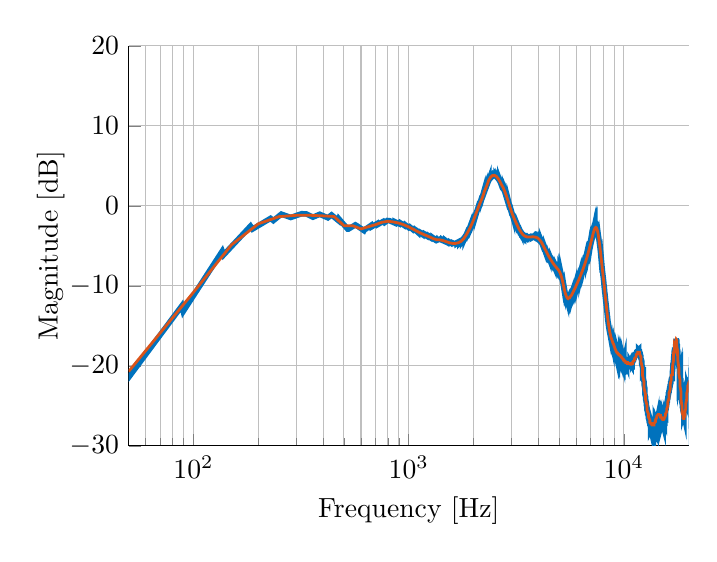
\begin{tikzpicture}

\begin{axis}[%
width=2.8in,
height=2in,
at={(1.457in,0.712in)},
scale only axis,
xmode=log,
xmin=50,
xmax=20000,
xminorticks=true,
xlabel={Frequency [Hz]},
xmajorgrids,
xminorgrids,
ylabel style={yshift=-0.5em},
%xlabel style={yshift=-0.2em},
ymin=-30,
ymax=20,
ylabel={Magnitude [dB]},
ymajorgrids,
axis background/.style={fill=white},
axis x line*=bottom,
axis y line*=left
]
\addplot [color=mycolor1,solid,forget plot, line width=2pt]
table[row sep=crcr]{%
	39.9	-24.3\\
	41.4	-24.4\\
	88.3	-12.5\\
	89.6	-13.2\\
	136	-5.67\\
	138	-6.14\\
	184	-2.53\\
	188	-2.91\\
	228	-1.57\\
	235	-1.85\\
	256	-1.04\\
	283	-1.46\\
	318	-0.988\\
	334	-1.01\\
	359	-1.42\\
	386	-1.06\\
	421	-1.5\\
	438	-1.14\\
	473	-1.88\\
	475	-1.67\\
	521	-2.92\\
	524	-2.92\\
	565	-2.38\\
	573	-2.47\\
	619	-3.09\\
	620	-3.05\\
	668	-2.45\\
	671	-2.64\\
	714	-2.21\\
	717	-2.35\\
	763	-1.94\\
	772	-2.1\\
	796	-1.84\\
	814	-1.86\\
	861	-2.15\\
	862	-1.98\\
	906	-2.27\\
	912	-2.12\\
	956	-2.48\\
	961	-2.36\\
	1e+03	-2.73\\
	1.01e+03	-2.63\\
	1.05e+03	-3.01\\
	1.06e+03	-2.9\\
	1.1e+03	-3.29\\
	1.1e+03	-3.18\\
	1.15e+03	-3.53\\
	1.15e+03	-3.43\\
	1.2e+03	-3.72\\
	1.2e+03	-3.62\\
	1.25e+03	-3.92\\
	1.25e+03	-3.82\\
	1.3e+03	-4.11\\
	1.3e+03	-4.01\\
	1.34e+03	-4.27\\
	1.35e+03	-4.17\\
	1.36e+03	-4.28\\
	1.39e+03	-4.17\\
	1.44e+03	-4.35\\
	1.44e+03	-4.25\\
	1.49e+03	-4.49\\
	1.49e+03	-4.38\\
	1.53e+03	-4.62\\
	1.54e+03	-4.5\\
	1.58e+03	-4.7\\
	1.59e+03	-4.6\\
	1.63e+03	-4.73\\
	1.64e+03	-4.73\\
	1.68e+03	-4.58\\
	1.68e+03	-4.68\\
	1.73e+03	-4.45\\
	1.73e+03	-4.56\\
	1.78e+03	-4.2\\
	1.78e+03	-4.3\\
	1.83e+03	-3.81\\
	1.83e+03	-3.91\\
	1.87e+03	-3.32\\
	1.88e+03	-3.41\\
	1.92e+03	-2.74\\
	1.92e+03	-2.83\\
	1.97e+03	-2.13\\
	1.97e+03	-2.22\\
	2.02e+03	-1.45\\
	2.02e+03	-1.5\\
	2.07e+03	-0.728\\
	2.07e+03	-0.781\\
	2.11e+03	-0.0306\\
	2.12e+03	-0.0878\\
	2.16e+03	0.637\\
	2.17e+03	0.578\\
	2.21e+03	1.34\\
	2.21e+03	1.26\\
	2.26e+03	2.05\\
	2.26e+03	1.99\\
	2.31e+03	2.63\\
	2.31e+03	2.59\\
	2.36e+03	3.27\\
	2.36e+03	3.21\\
	2.4e+03	3.65\\
	2.41e+03	3.58\\
	2.45e+03	3.85\\
	2.46e+03	3.77\\
	2.48e+03	3.88\\
	2.5e+03	3.85\\
	2.55e+03	3.64\\
	2.55e+03	3.72\\
	2.6e+03	3.4\\
	2.6e+03	3.46\\
	2.65e+03	3.07\\
	2.65e+03	3.12\\
	2.69e+03	2.64\\
	2.7e+03	2.7\\
	2.74e+03	2.28\\
	2.75e+03	2.35\\
	2.79e+03	1.79\\
	2.79e+03	1.86\\
	2.84e+03	1.26\\
	2.84e+03	1.28\\
	2.89e+03	0.657\\
	2.89e+03	0.687\\
	2.94e+03	0.0378\\
	2.94e+03	0.0693\\
	2.98e+03	-0.551\\
	2.99e+03	-0.504\\
	3.03e+03	-1.07\\
	3.03e+03	-1.03\\
	3.08e+03	-1.55\\
	3.08e+03	-1.51\\
	3.13e+03	-1.97\\
	3.13e+03	-1.93\\
	3.18e+03	-2.36\\
	3.18e+03	-2.32\\
	3.23e+03	-2.72\\
	3.23e+03	-2.67\\
	3.27e+03	-3.03\\
	3.28e+03	-2.99\\
	3.32e+03	-3.31\\
	3.32e+03	-3.26\\
	3.37e+03	-3.55\\
	3.37e+03	-3.49\\
	3.42e+03	-3.74\\
	3.42e+03	-3.68\\
	3.47e+03	-3.84\\
	3.47e+03	-3.78\\
	3.52e+03	-3.91\\
	3.52e+03	-3.85\\
	3.56e+03	-3.94\\
	3.57e+03	-3.88\\
	3.6e+03	-3.96\\
	3.62e+03	-3.95\\
	3.66e+03	-3.88\\
	3.67e+03	-3.95\\
	3.71e+03	-3.87\\
	3.72e+03	-3.87\\
	3.74e+03	-3.94\\
	3.77e+03	-3.87\\
	3.77e+03	-3.95\\
	3.81e+03	-3.88\\
	3.85e+03	-3.96\\
	3.86e+03	-3.9\\
	3.9e+03	-4\\
	3.91e+03	-3.94\\
	3.95e+03	-4.06\\
	3.95e+03	-4\\
	4e+03	-4.15\\
	4e+03	-4.1\\
	4.05e+03	-4.28\\
	4.05e+03	-4.25\\
	4.1e+03	-4.45\\
	4.1e+03	-4.42\\
	4.15e+03	-4.67\\
	4.15e+03	-4.62\\
	4.19e+03	-4.92\\
	4.2e+03	-4.87\\
	4.24e+03	-5.18\\
	4.24e+03	-5.13\\
	4.29e+03	-5.46\\
	4.29e+03	-5.41\\
	4.34e+03	-5.69\\
	4.34e+03	-5.65\\
	4.38e+03	-5.95\\
	4.39e+03	-5.88\\
	4.43e+03	-6.19\\
	4.44e+03	-6.15\\
	4.48e+03	-6.43\\
	4.48e+03	-6.37\\
	4.53e+03	-6.64\\
	4.53e+03	-6.6\\
	4.58e+03	-6.85\\
	4.58e+03	-6.8\\
	4.63e+03	-7.04\\
	4.63e+03	-6.98\\
	4.67e+03	-7.23\\
	4.68e+03	-7.16\\
	4.72e+03	-7.4\\
	4.72e+03	-7.34\\
	4.77e+03	-7.55\\
	4.78e+03	-7.49\\
	4.82e+03	-7.7\\
	4.82e+03	-7.64\\
	4.87e+03	-7.83\\
	4.87e+03	-7.77\\
	4.91e+03	-7.97\\
	4.92e+03	-7.9\\
	4.96e+03	-8.11\\
	4.97e+03	-8.05\\
	5.01e+03	-8.29\\
	5.02e+03	-8.23\\
	5.06e+03	-8.52\\
	5.06e+03	-8.46\\
	5.11e+03	-8.82\\
	5.11e+03	-8.76\\
	5.16e+03	-9.22\\
	5.16e+03	-9.14\\
	5.21e+03	-9.68\\
	5.21e+03	-9.63\\
	5.25e+03	-10.2\\
	5.26e+03	-10.1\\
	5.3e+03	-10.7\\
	5.31e+03	-10.6\\
	5.35e+03	-11.1\\
	5.35e+03	-11\\
	5.4e+03	-11.4\\
	5.4e+03	-11.3\\
	5.45e+03	-11.6\\
	5.45e+03	-11.5\\
	5.5e+03	-11.6\\
	5.52e+03	-11.6\\
	5.54e+03	-11.5\\
	5.55e+03	-11.6\\
	5.59e+03	-11.4\\
	5.6e+03	-11.5\\
	5.64e+03	-11.3\\
	5.64e+03	-11.4\\
	5.69e+03	-11.1\\
	5.69e+03	-11.2\\
	5.74e+03	-11\\
	5.74e+03	-11.1\\
	5.79e+03	-10.8\\
	5.79e+03	-10.9\\
	5.83e+03	-10.6\\
	5.84e+03	-10.7\\
	5.88e+03	-10.4\\
	5.88e+03	-10.5\\
	5.93e+03	-10.2\\
	5.93e+03	-10.3\\
	5.98e+03	-9.98\\
	5.98e+03	-10.1\\
	6.03e+03	-9.79\\
	6.03e+03	-9.87\\
	6.07e+03	-9.59\\
	6.08e+03	-9.66\\
	6.13e+03	-9.37\\
	6.13e+03	-9.45\\
	6.17e+03	-9.15\\
	6.17e+03	-9.24\\
	6.22e+03	-8.93\\
	6.22e+03	-9.02\\
	6.27e+03	-8.71\\
	6.27e+03	-8.79\\
	6.32e+03	-8.49\\
	6.32e+03	-8.57\\
	6.36e+03	-8.25\\
	6.37e+03	-8.34\\
	6.41e+03	-8.01\\
	6.42e+03	-8.12\\
	6.46e+03	-7.78\\
	6.47e+03	-7.87\\
	6.51e+03	-7.55\\
	6.51e+03	-7.63\\
	6.56e+03	-7.29\\
	6.56e+03	-7.38\\
	6.61e+03	-7.04\\
	6.61e+03	-7.13\\
	6.65e+03	-6.77\\
	6.66e+03	-6.87\\
	6.7e+03	-6.5\\
	6.71e+03	-6.59\\
	6.75e+03	-6.22\\
	6.76e+03	-6.31\\
	6.8e+03	-5.92\\
	6.8e+03	-6.02\\
	6.85e+03	-5.63\\
	6.85e+03	-5.72\\
	6.9e+03	-5.33\\
	6.9e+03	-5.42\\
	6.94e+03	-5\\
	6.95e+03	-5.1\\
	6.99e+03	-4.68\\
	7e+03	-4.78\\
	7.04e+03	-4.36\\
	7.04e+03	-4.46\\
	7.09e+03	-4.05\\
	7.09e+03	-4.14\\
	7.14e+03	-3.74\\
	7.14e+03	-3.82\\
	7.19e+03	-3.43\\
	7.19e+03	-3.51\\
	7.24e+03	-3.15\\
	7.24e+03	-3.24\\
	7.28e+03	-2.92\\
	7.29e+03	-3\\
	7.33e+03	-2.75\\
	7.33e+03	-2.82\\
	7.38e+03	-2.65\\
	7.39e+03	-2.74\\
	7.41e+03	-2.64\\
	7.43e+03	-2.66\\
	7.47e+03	-2.85\\
	7.48e+03	-2.79\\
	7.53e+03	-3.09\\
	7.53e+03	-3.03\\
	7.57e+03	-3.43\\
	7.58e+03	-3.38\\
	7.62e+03	-3.87\\
	7.62e+03	-3.82\\
	7.67e+03	-4.38\\
	7.67e+03	-4.35\\
	7.72e+03	-4.99\\
	7.72e+03	-4.95\\
	7.77e+03	-5.63\\
	7.77e+03	-5.58\\
	7.81e+03	-6.28\\
	7.82e+03	-6.22\\
	7.86e+03	-6.93\\
	7.87e+03	-6.9\\
	7.91e+03	-7.58\\
	7.91e+03	-7.57\\
	7.96e+03	-8.27\\
	7.96e+03	-8.24\\
	8.01e+03	-8.93\\
	8.01e+03	-8.88\\
	8.06e+03	-9.57\\
	8.06e+03	-9.52\\
	8.1e+03	-10.2\\
	8.11e+03	-10.2\\
	8.15e+03	-10.9\\
	8.15e+03	-10.8\\
	8.2e+03	-11.5\\
	8.2e+03	-11.5\\
	8.25e+03	-12.2\\
	8.25e+03	-12.1\\
	8.3e+03	-12.8\\
	8.3e+03	-12.8\\
	8.35e+03	-13.4\\
	8.35e+03	-13.4\\
	8.39e+03	-14\\
	8.4e+03	-14\\
	8.44e+03	-14.6\\
	8.44e+03	-14.6\\
	8.49e+03	-15.1\\
	8.49e+03	-15.1\\
	8.54e+03	-15.5\\
	8.54e+03	-15.5\\
	8.59e+03	-15.9\\
	8.59e+03	-15.9\\
	8.64e+03	-16.2\\
	8.64e+03	-16.2\\
	8.68e+03	-16.5\\
	8.69e+03	-16.4\\
	8.73e+03	-16.7\\
	8.73e+03	-16.7\\
	8.78e+03	-17\\
	8.78e+03	-16.9\\
	8.83e+03	-17.1\\
	8.83e+03	-17.1\\
	8.88e+03	-17.3\\
	8.88e+03	-17.2\\
	8.92e+03	-17.5\\
	8.93e+03	-17.4\\
	8.97e+03	-17.7\\
	8.98e+03	-17.6\\
	9.02e+03	-17.9\\
	9.02e+03	-17.8\\
	9.07e+03	-18\\
	9.07e+03	-18\\
	9.12e+03	-18.2\\
	9.12e+03	-18.1\\
	9.17e+03	-18.4\\
	9.17e+03	-18.3\\
	9.21e+03	-18.5\\
	9.22e+03	-18.4\\
	9.26e+03	-18.6\\
	9.27e+03	-18.5\\
	9.31e+03	-18.7\\
	9.31e+03	-18.6\\
	9.36e+03	-18.7\\
	9.36e+03	-18.6\\
	9.4e+03	-18.8\\
	9.41e+03	-18.7\\
	9.46e+03	-18.8\\
	9.48e+03	-18.7\\
	9.5e+03	-18.9\\
	9.51e+03	-18.8\\
	9.55e+03	-18.9\\
	9.56e+03	-18.8\\
	9.6e+03	-19\\
	9.61e+03	-18.9\\
	9.65e+03	-19\\
	9.65e+03	-18.9\\
	9.69e+03	-19.1\\
	9.7e+03	-19\\
	9.74e+03	-19.2\\
	9.75e+03	-19\\
	9.8e+03	-19.2\\
	9.8e+03	-19.1\\
	9.84e+03	-19.3\\
	9.84e+03	-19.2\\
	9.89e+03	-19.4\\
	9.89e+03	-19.2\\
	9.94e+03	-19.5\\
	9.94e+03	-19.3\\
	9.98e+03	-19.5\\
	1e+04	-19.4\\
	1e+04	-19.6\\
	1e+04	-19.4\\
	1.01e+04	-19.6\\
	1.01e+04	-19.4\\
	1.01e+04	-19.7\\
	1.01e+04	-19.5\\
	1.02e+04	-19.7\\
	1.02e+04	-19.5\\
	1.02e+04	-19.8\\
	1.02e+04	-19.5\\
	1.03e+04	-19.8\\
	1.03e+04	-19.8\\
	1.03e+04	-19.5\\
	1.04e+04	-19.5\\
	1.04e+04	-19.8\\
	1.04e+04	-19.8\\
	1.04e+04	-19.6\\
	1.05e+04	-19.6\\
	1.05e+04	-19.8\\
	1.05e+04	-19.6\\
	1.05e+04	-19.8\\
	1.05e+04	-19.6\\
	1.05e+04	-19.8\\
	1.06e+04	-19.6\\
	1.06e+04	-19.8\\
	1.06e+04	-19.6\\
	1.06e+04	-19.8\\
	1.07e+04	-19.6\\
	1.07e+04	-19.8\\
	1.07e+04	-19.8\\
	1.07e+04	-19.6\\
	1.08e+04	-19.8\\
	1.08e+04	-19.6\\
	1.08e+04	-19.8\\
	1.08e+04	-19.6\\
	1.09e+04	-19.7\\
	1.09e+04	-19.5\\
	1.09e+04	-19.6\\
	1.1e+04	-19.5\\
	1.1e+04	-19.6\\
	1.1e+04	-19.4\\
	1.1e+04	-19.5\\
	1.11e+04	-19.3\\
	1.11e+04	-19.4\\
	1.11e+04	-19.2\\
	1.11e+04	-19.3\\
	1.11e+04	-19.1\\
	1.11e+04	-19.2\\
	1.12e+04	-19\\
	1.12e+04	-19.1\\
	1.12e+04	-18.9\\
	1.12e+04	-18.9\\
	1.13e+04	-18.8\\
	1.13e+04	-18.8\\
	1.13e+04	-18.6\\
	1.13e+04	-18.7\\
	1.14e+04	-18.5\\
	1.14e+04	-18.5\\
	1.14e+04	-18.4\\
	1.14e+04	-18.4\\
	1.15e+04	-18.3\\
	1.15e+04	-18.3\\
	1.15e+04	-18.2\\
	1.15e+04	-18.2\\
	1.16e+04	-18.1\\
	1.16e+04	-18.2\\
	1.16e+04	-18\\
	1.16e+04	-18.1\\
	1.17e+04	-18\\
	1.17e+04	-18.1\\
	1.17e+04	-18\\
	1.17e+04	-18\\
	1.18e+04	-18.1\\
	1.18e+04	-18.1\\
	1.18e+04	-18.2\\
	1.18e+04	-18.2\\
	1.19e+04	-18.4\\
	1.19e+04	-18.3\\
	1.19e+04	-18.5\\
	1.19e+04	-18.5\\
	1.2e+04	-18.8\\
	1.2e+04	-18.7\\
	1.2e+04	-19.1\\
	1.2e+04	-19.1\\
	1.21e+04	-19.4\\
	1.21e+04	-19.4\\
	1.21e+04	-19.8\\
	1.21e+04	-19.8\\
	1.22e+04	-20.2\\
	1.22e+04	-20.2\\
	1.22e+04	-20.7\\
	1.22e+04	-20.6\\
	1.22e+04	-21.1\\
	1.23e+04	-21\\
	1.23e+04	-21.5\\
	1.23e+04	-21.5\\
	1.24e+04	-22\\
	1.24e+04	-21.9\\
	1.24e+04	-22.4\\
	1.24e+04	-22.3\\
	1.25e+04	-22.8\\
	1.25e+04	-22.7\\
	1.25e+04	-23.2\\
	1.25e+04	-23.1\\
	1.25e+04	-23.6\\
	1.25e+04	-23.5\\
	1.26e+04	-23.9\\
	1.26e+04	-23.8\\
	1.26e+04	-24.2\\
	1.26e+04	-24.1\\
	1.27e+04	-24.6\\
	1.27e+04	-24.5\\
	1.27e+04	-24.9\\
	1.27e+04	-24.8\\
	1.28e+04	-25.3\\
	1.28e+04	-25.2\\
	1.28e+04	-25.6\\
	1.28e+04	-25.5\\
	1.29e+04	-25.9\\
	1.29e+04	-25.8\\
	1.29e+04	-26.2\\
	1.29e+04	-26\\
	1.3e+04	-26.4\\
	1.3e+04	-26.3\\
	1.3e+04	-26.7\\
	1.3e+04	-26.5\\
	1.31e+04	-26.9\\
	1.31e+04	-26.7\\
	1.31e+04	-27.1\\
	1.31e+04	-27\\
	1.32e+04	-27.3\\
	1.32e+04	-27.1\\
	1.32e+04	-27.5\\
	1.32e+04	-27.3\\
	1.33e+04	-27.6\\
	1.33e+04	-27.4\\
	1.33e+04	-27.7\\
	1.33e+04	-27.5\\
	1.33e+04	-27.8\\
	1.34e+04	-27.6\\
	1.34e+04	-27.9\\
	1.34e+04	-27.6\\
	1.35e+04	-27.9\\
	1.35e+04	-27.7\\
	1.35e+04	-28\\
	1.35e+04	-27.8\\
	1.36e+04	-28\\
	1.36e+04	-27.8\\
	1.36e+04	-28.1\\
	1.36e+04	-27.8\\
	1.37e+04	-28.1\\
	1.37e+04	-28.1\\
	1.37e+04	-27.9\\
	1.37e+04	-28.2\\
	1.37e+04	-27.9\\
	1.38e+04	-27.8\\
	1.38e+04	-28.1\\
	1.38e+04	-28.2\\
	1.38e+04	-27.8\\
	1.39e+04	-28\\
	1.39e+04	-27.8\\
	1.39e+04	-28\\
	1.39e+04	-27.6\\
	1.39e+04	-27.9\\
	1.4e+04	-27.6\\
	1.4e+04	-27.8\\
	1.4e+04	-27.4\\
	1.41e+04	-27.7\\
	1.41e+04	-27.3\\
	1.41e+04	-27.6\\
	1.41e+04	-27.2\\
	1.41e+04	-27.5\\
	1.42e+04	-27.1\\
	1.42e+04	-27.3\\
	1.42e+04	-27\\
	1.43e+04	-27.2\\
	1.43e+04	-26.9\\
	1.43e+04	-27.2\\
	1.43e+04	-26.9\\
	1.43e+04	-27.1\\
	1.44e+04	-26.8\\
	1.44e+04	-27\\
	1.44e+04	-26.7\\
	1.45e+04	-26.8\\
	1.45e+04	-27.1\\
	1.45e+04	-27.1\\
	1.45e+04	-26.7\\
	1.45e+04	-27.1\\
	1.46e+04	-26.8\\
	1.46e+04	-26.8\\
	1.46e+04	-27\\
	1.46e+04	-27.2\\
	1.47e+04	-26.8\\
	1.47e+04	-26.8\\
	1.47e+04	-27.1\\
	1.47e+04	-27.2\\
	1.47e+04	-26.9\\
	1.48e+04	-26.9\\
	1.48e+04	-27.2\\
	1.48e+04	-27.2\\
	1.49e+04	-26.9\\
	1.49e+04	-27\\
	1.49e+04	-27.3\\
	1.49e+04	-27\\
	1.49e+04	-27.3\\
	1.5e+04	-27\\
	1.5e+04	-27.3\\
	1.5e+04	-27.1\\
	1.5e+04	-27.3\\
	1.51e+04	-27.3\\
	1.51e+04	-27.1\\
	1.51e+04	-27\\
	1.52e+04	-27.3\\
	1.52e+04	-27.3\\
	1.52e+04	-27\\
	1.52e+04	-27.2\\
	1.52e+04	-27\\
	1.53e+04	-27.1\\
	1.53e+04	-26.9\\
	1.53e+04	-27\\
	1.53e+04	-26.7\\
	1.54e+04	-26.9\\
	1.54e+04	-26.5\\
	1.54e+04	-26.7\\
	1.54e+04	-26.4\\
	1.55e+04	-26.5\\
	1.55e+04	-26.2\\
	1.55e+04	-26.3\\
	1.55e+04	-26\\
	1.56e+04	-26.1\\
	1.56e+04	-25.8\\
	1.56e+04	-25.9\\
	1.56e+04	-25.5\\
	1.56e+04	-25.8\\
	1.57e+04	-25.3\\
	1.57e+04	-25.5\\
	1.57e+04	-25.1\\
	1.57e+04	-25.4\\
	1.58e+04	-24.8\\
	1.58e+04	-25.1\\
	1.58e+04	-24.7\\
	1.58e+04	-24.9\\
	1.59e+04	-24.4\\
	1.59e+04	-24.6\\
	1.59e+04	-24.2\\
	1.59e+04	-24.4\\
	1.6e+04	-24\\
	1.6e+04	-24.2\\
	1.6e+04	-23.8\\
	1.6e+04	-24\\
	1.61e+04	-23.6\\
	1.61e+04	-23.8\\
	1.61e+04	-23.3\\
	1.61e+04	-23.6\\
	1.62e+04	-23.1\\
	1.62e+04	-23.4\\
	1.62e+04	-23\\
	1.62e+04	-23.2\\
	1.63e+04	-22.8\\
	1.63e+04	-23\\
	1.63e+04	-22.6\\
	1.63e+04	-22.9\\
	1.64e+04	-22.4\\
	1.64e+04	-22.7\\
	1.64e+04	-22.3\\
	1.64e+04	-22.5\\
	1.65e+04	-22.1\\
	1.65e+04	-22.3\\
	1.65e+04	-21.9\\
	1.65e+04	-22.1\\
	1.66e+04	-21.7\\
	1.66e+04	-21.9\\
	1.66e+04	-21.5\\
	1.66e+04	-21.8\\
	1.67e+04	-21.4\\
	1.67e+04	-21.7\\
	1.67e+04	-21.4\\
	1.67e+04	-21.4\\
	1.67e+04	-21.6\\
	1.68e+04	-21.6\\
	1.68e+04	-21.1\\
	1.68e+04	-21.3\\
	1.68e+04	-20.6\\
	1.68e+04	-20.8\\
	1.69e+04	-20.1\\
	1.69e+04	-20.3\\
	1.69e+04	-19.7\\
	1.69e+04	-19.9\\
	1.7e+04	-19.3\\
	1.7e+04	-19.5\\
	1.7e+04	-18.9\\
	1.7e+04	-19.1\\
	1.71e+04	-18.5\\
	1.71e+04	-18.7\\
	1.71e+04	-18.1\\
	1.71e+04	-18.3\\
	1.72e+04	-17.9\\
	1.72e+04	-18.1\\
	1.72e+04	-17.8\\
	1.72e+04	-17.7\\
	1.73e+04	-18.1\\
	1.73e+04	-17.9\\
	1.73e+04	-18.4\\
	1.73e+04	-18.4\\
	1.74e+04	-17.9\\
	1.74e+04	-18.2\\
	1.74e+04	-17.3\\
	1.74e+04	-17.5\\
	1.75e+04	-16.8\\
	1.75e+04	-17\\
	1.75e+04	-16.7\\
	1.75e+04	-16.6\\
	1.76e+04	-17\\
	1.76e+04	-16.7\\
	1.76e+04	-17.2\\
	1.76e+04	-17\\
	1.77e+04	-17.6\\
	1.77e+04	-17.3\\
	1.77e+04	-18\\
	1.77e+04	-17.7\\
	1.78e+04	-18.4\\
	1.78e+04	-18.1\\
	1.78e+04	-18.8\\
	1.78e+04	-18.5\\
	1.79e+04	-19.2\\
	1.79e+04	-18.9\\
	1.79e+04	-19.5\\
	1.79e+04	-19.3\\
	1.8e+04	-19.9\\
	1.8e+04	-19.6\\
	1.8e+04	-20.2\\
	1.8e+04	-19.9\\
	1.81e+04	-20.5\\
	1.81e+04	-20.3\\
	1.81e+04	-20.9\\
	1.81e+04	-20.6\\
	1.81e+04	-21.2\\
	1.82e+04	-20.9\\
	1.82e+04	-21.5\\
	1.82e+04	-21.2\\
	1.82e+04	-21.8\\
	1.83e+04	-21.5\\
	1.83e+04	-22.1\\
	1.83e+04	-21.9\\
	1.83e+04	-22.5\\
	1.83e+04	-22.2\\
	1.84e+04	-22.9\\
	1.84e+04	-22.6\\
	1.84e+04	-23.3\\
	1.84e+04	-23\\
	1.85e+04	-23.7\\
	1.85e+04	-23.4\\
	1.85e+04	-24\\
	1.85e+04	-23.9\\
	1.86e+04	-24.4\\
	1.86e+04	-24.2\\
	1.86e+04	-24.7\\
	1.86e+04	-24.5\\
	1.87e+04	-25\\
	1.87e+04	-24.8\\
	1.87e+04	-25.3\\
	1.87e+04	-25\\
	1.88e+04	-25.5\\
	1.88e+04	-25.3\\
	1.88e+04	-25.7\\
	1.88e+04	-25.5\\
	1.89e+04	-25.8\\
	1.89e+04	-25.5\\
	1.89e+04	-25.8\\
	1.89e+04	-25.9\\
	1.89e+04	-25.6\\
	1.9e+04	-25.9\\
	1.9e+04	-25.6\\
	1.9e+04	-25.8\\
	1.91e+04	-25.6\\
	1.91e+04	-25.8\\
	1.91e+04	-25.5\\
	1.91e+04	-25.4\\
	1.91e+04	-25.7\\
	1.92e+04	-25.6\\
	1.92e+04	-25.3\\
	1.92e+04	-25.5\\
	1.93e+04	-25.1\\
	1.93e+04	-25.3\\
	1.93e+04	-24.8\\
	1.93e+04	-25.1\\
	1.94e+04	-24.7\\
	1.94e+04	-24.9\\
	1.94e+04	-24.5\\
	1.94e+04	-24.7\\
	1.94e+04	-24.3\\
	1.95e+04	-24.5\\
	1.95e+04	-24.1\\
	1.95e+04	-24.3\\
	1.95e+04	-23.9\\
	1.96e+04	-24.1\\
	1.96e+04	-23.7\\
	1.96e+04	-23.8\\
	1.96e+04	-23.5\\
	1.97e+04	-23.6\\
	1.97e+04	-23.3\\
	1.97e+04	-23.5\\
	1.97e+04	-23.2\\
	1.97e+04	-23.3\\
	1.98e+04	-23\\
	1.98e+04	-23.3\\
	1.98e+04	-22.9\\
	1.99e+04	-23.1\\
	1.99e+04	-22.9\\
	1.99e+04	-23\\
	1.99e+04	-22.8\\
	2e+04	-22.7\\
	2e+04	-23\\
	2e+04	-22.6\\
	2e+04	-23.1\\
	2.01e+04	-23.2\\
	2.01e+04	-22.4\\
	2.01e+04	-22.5\\
	2.01e+04	-23.6\\
	2.02e+04	-23.8\\
	2.02e+04	-21.9\\
	2.02e+04	-24.1\\
	2.02e+04	-22.1\\
	2.02e+04	-24.2\\
	2.03e+04	-21.9\\
	2.03e+04	-22.1\\
	2.03e+04	-24.6\\
	2.03e+04	-25.1\\
	2.03e+04	-21.8\\
	2.04e+04	-21.4\\
	2.04e+04	-25.1\\
	2.04e+04	-25.7\\
	2.05e+04	-20.1\\
	2.05e+04	-20.7\\
	2.05e+04	-27.2\\
	2.06e+04	-28.4\\
	2.06e+04	-20.6\\
	2.06e+04	-18.9\\
	2.06e+04	-26.9\\
	2.06e+04	-19.9\\
	2.06e+04	-32.7\\
	2.07e+04	-26.7\\
	2.07e+04	-18.8\\
	2.07e+04	-39.7\\
	2.07e+04	-19.4\\
	2.08e+04	-29.9\\
	2.08e+04	-19.8\\
	2.08e+04	-34\\
	2.09e+04	-17.1\\
	2.09e+04	-32.1\\
	2.09e+04	-16.6\\
	2.09e+04	-16.6\\
	2.09e+04	-31\\
	2.1e+04	-22.6\\
};
\addplot [color=mycolor2,solid,forget plot, line width=1pt]
table[row sep=crcr]{%
	0	-57.4\\
	50	-20.7\\
	100	-10.8\\
	150	-4.89\\
	200	-2.25\\
	250	-1.35\\
	300	-1.19\\
	350	-1.19\\
	400	-1.26\\
	450	-1.33\\
	500	-2.48\\
	550	-2.5\\
	600	-2.89\\
	650	-2.61\\
	700	-2.36\\
	750	-2.06\\
	800	-1.93\\
	850	-2.02\\
	900	-2.16\\
	950	-2.38\\
	1e+03	-2.64\\
	1.05e+03	-2.93\\
	1.1e+03	-3.22\\
	1.15e+03	-3.48\\
	1.2e+03	-3.69\\
	1.25e+03	-3.89\\
	1.3e+03	-4.1\\
	1.35e+03	-4.24\\
	1.4e+03	-4.26\\
	1.45e+03	-4.36\\
	1.5e+03	-4.5\\
	1.55e+03	-4.63\\
	1.6e+03	-4.7\\
	1.65e+03	-4.7\\
	1.7e+03	-4.62\\
	1.75e+03	-4.45\\
	1.8e+03	-4.11\\
	1.85e+03	-3.64\\
	1.9e+03	-3.09\\
	1.95e+03	-2.48\\
	2e+03	-1.79\\
	2.05e+03	-1.03\\
	2.1e+03	-0.297\\
	2.15e+03	0.416\\
	2.2e+03	1.03\\
	2.25e+03	1.85\\
	2.3e+03	2.45\\
	2.35e+03	3.15\\
	2.4e+03	3.57\\
	2.45e+03	3.79\\
	2.5e+03	3.81\\
	2.55e+03	3.69\\
	2.6e+03	3.42\\
	2.65e+03	3.07\\
	2.7e+03	2.63\\
	2.75e+03	2.25\\
	2.8e+03	1.73\\
	2.85e+03	1.16\\
	2.9e+03	0.528\\
	2.95e+03	-0.11\\
	3e+03	-0.701\\
	3.05e+03	-1.22\\
	3.1e+03	-1.68\\
	3.15e+03	-2.1\\
	3.2e+03	-2.49\\
	3.25e+03	-2.85\\
	3.3e+03	-3.15\\
	3.35e+03	-3.41\\
	3.4e+03	-3.62\\
	3.45e+03	-3.76\\
	3.5e+03	-3.84\\
	3.55e+03	-3.89\\
	3.6e+03	-3.9\\
	3.65e+03	-3.9\\
	3.7e+03	-3.89\\
	3.75e+03	-3.88\\
	3.8e+03	-3.88\\
	3.85e+03	-3.9\\
	3.9e+03	-3.93\\
	3.95e+03	-3.99\\
	4e+03	-4.09\\
	4.05e+03	-4.23\\
	4.1e+03	-4.41\\
	4.15e+03	-4.62\\
	4.2e+03	-4.88\\
	4.25e+03	-5.16\\
	4.3e+03	-5.43\\
	4.35e+03	-5.68\\
	4.4e+03	-5.94\\
	4.45e+03	-6.2\\
	4.5e+03	-6.43\\
	4.55e+03	-6.65\\
	4.6e+03	-6.85\\
	4.65e+03	-7.05\\
	4.7e+03	-7.23\\
	4.75e+03	-7.41\\
	4.8e+03	-7.56\\
	4.85e+03	-7.7\\
	4.9e+03	-7.84\\
	4.95e+03	-7.99\\
	5e+03	-8.16\\
	5.05e+03	-8.39\\
	5.1e+03	-8.69\\
	5.15e+03	-9.08\\
	5.2e+03	-9.56\\
	5.25e+03	-10.1\\
	5.3e+03	-10.6\\
	5.35e+03	-11\\
	5.4e+03	-11.3\\
	5.45e+03	-11.5\\
	5.5e+03	-11.6\\
	5.55e+03	-11.5\\
	5.6e+03	-11.5\\
	5.65e+03	-11.3\\
	5.7e+03	-11.2\\
	5.75e+03	-11\\
	5.8e+03	-10.8\\
	5.85e+03	-10.6\\
	5.9e+03	-10.4\\
	5.95e+03	-10.2\\
	6e+03	-9.96\\
	6.05e+03	-9.75\\
	6.1e+03	-9.54\\
	6.15e+03	-9.32\\
	6.2e+03	-9.1\\
	6.25e+03	-8.88\\
	6.3e+03	-8.65\\
	6.35e+03	-8.41\\
	6.4e+03	-8.18\\
	6.45e+03	-7.94\\
	6.5e+03	-7.69\\
	6.55e+03	-7.43\\
	6.6e+03	-7.17\\
	6.65e+03	-6.9\\
	6.7e+03	-6.62\\
	6.75e+03	-6.33\\
	6.8e+03	-6.03\\
	6.85e+03	-5.72\\
	6.9e+03	-5.4\\
	6.95e+03	-5.07\\
	7e+03	-4.74\\
	7.05e+03	-4.41\\
	7.1e+03	-4.07\\
	7.15e+03	-3.75\\
	7.2e+03	-3.43\\
	7.25e+03	-3.15\\
	7.3e+03	-2.92\\
	7.35e+03	-2.77\\
	7.4e+03	-2.7\\
	7.45e+03	-2.75\\
	7.5e+03	-2.93\\
	7.55e+03	-3.22\\
	7.6e+03	-3.63\\
	7.65e+03	-4.14\\
	7.7e+03	-4.72\\
	7.75e+03	-5.35\\
	7.8e+03	-6.01\\
	7.85e+03	-6.69\\
	7.9e+03	-7.37\\
	7.95e+03	-8.05\\
	8e+03	-8.73\\
	8.05e+03	-9.39\\
	8.1e+03	-10\\
	8.15e+03	-10.7\\
	8.2e+03	-11.4\\
	8.25e+03	-12\\
	8.3e+03	-12.7\\
	8.35e+03	-13.4\\
	8.4e+03	-14\\
	8.45e+03	-14.5\\
	8.5e+03	-15\\
	8.55e+03	-15.4\\
	8.6e+03	-15.8\\
	8.65e+03	-16.1\\
	8.7e+03	-16.4\\
	8.75e+03	-16.6\\
	8.8e+03	-16.8\\
	8.85e+03	-17\\
	8.9e+03	-17.2\\
	8.95e+03	-17.3\\
	9e+03	-17.5\\
	9.05e+03	-17.7\\
	9.1e+03	-17.9\\
	9.15e+03	-18\\
	9.2e+03	-18.2\\
	9.25e+03	-18.3\\
	9.3e+03	-18.4\\
	9.35e+03	-18.4\\
	9.4e+03	-18.5\\
	9.45e+03	-18.6\\
	9.5e+03	-18.6\\
	9.55e+03	-18.7\\
	9.6e+03	-18.7\\
	9.65e+03	-18.8\\
	9.7e+03	-18.9\\
	9.75e+03	-18.9\\
	9.8e+03	-19\\
	9.85e+03	-19.1\\
	9.9e+03	-19.2\\
	9.95e+03	-19.2\\
	1e+04	-19.3\\
	1.00e+04	-19.4\\
	1.01e+04	-19.4\\
	1.02e+04	-19.5\\
	1.02e+04	-19.5\\
	1.02e+04	-19.6\\
	1.03e+04	-19.6\\
	1.04e+04	-19.6\\
	1.04e+04	-19.7\\
	1.04e+04	-19.7\\
	1.05e+04	-19.7\\
	1.06e+04	-19.7\\
	1.06e+04	-19.7\\
	1.06e+04	-19.7\\
	1.07e+04	-19.8\\
	1.08e+04	-19.8\\
	1.08e+04	-19.8\\
	1.08e+04	-19.7\\
	1.09e+04	-19.7\\
	1.1e+04	-19.7\\
	1.1e+04	-19.6\\
	1.10e+04	-19.5\\
	1.11e+04	-19.4\\
	1.12e+04	-19.3\\
	1.12e+04	-19.2\\
	1.12e+04	-19.1\\
	1.13e+04	-19\\
	1.14e+04	-18.8\\
	1.14e+04	-18.7\\
	1.14e+04	-18.6\\
	1.15e+04	-18.5\\
	1.16e+04	-18.4\\
	1.16e+04	-18.4\\
	1.16e+04	-18.3\\
	1.17e+04	-18.3\\
	1.18e+04	-18.3\\
	1.18e+04	-18.4\\
	1.18e+04	-18.5\\
	1.19e+04	-18.7\\
	1.2e+04	-18.9\\
	1.2e+04	-19.2\\
	1.20e+04	-19.5\\
	1.21e+04	-19.9\\
	1.22e+04	-20.3\\
	1.22e+04	-20.7\\
	1.22e+04	-21.2\\
	1.23e+04	-21.6\\
	1.24e+04	-22\\
	1.24e+04	-22.4\\
	1.24e+04	-22.8\\
	1.25e+04	-23.2\\
	1.26e+04	-23.6\\
	1.26e+04	-23.9\\
	1.26e+04	-24.2\\
	1.27e+04	-24.6\\
	1.28e+04	-24.9\\
	1.28e+04	-25.2\\
	1.28e+04	-25.5\\
	1.29e+04	-25.8\\
	1.3e+04	-26\\
	1.3e+04	-26.2\\
	1.30e+04	-26.4\\
	1.31e+04	-26.6\\
	1.32e+04	-26.8\\
	1.32e+04	-27\\
	1.32e+04	-27.1\\
	1.33e+04	-27.2\\
	1.34e+04	-27.2\\
	1.34e+04	-27.3\\
	1.34e+04	-27.3\\
	1.35e+04	-27.4\\
	1.36e+04	-27.4\\
	1.36e+04	-27.4\\
	1.36e+04	-27.4\\
	1.37e+04	-27.4\\
	1.38e+04	-27.4\\
	1.38e+04	-27.3\\
	1.38e+04	-27.2\\
	1.39e+04	-27.1\\
	1.4e+04	-27\\
	1.4e+04	-26.9\\
	1.40e+04	-26.8\\
	1.41e+04	-26.6\\
	1.42e+04	-26.5\\
	1.42e+04	-26.4\\
	1.42e+04	-26.3\\
	1.43e+04	-26.2\\
	1.44e+04	-26.1\\
	1.44e+04	-26.1\\
	1.44e+04	-26.1\\
	1.45e+04	-26.1\\
	1.46e+04	-26.1\\
	1.46e+04	-26.1\\
	1.46e+04	-26.1\\
	1.47e+04	-26.2\\
	1.48e+04	-26.2\\
	1.48e+04	-26.3\\
	1.48e+04	-26.4\\
	1.49e+04	-26.4\\
	1.5e+04	-26.5\\
	1.5e+04	-26.6\\
	1.50e+04	-26.6\\
	1.51e+04	-26.7\\
	1.52e+04	-26.7\\
	1.52e+04	-26.7\\
	1.52e+04	-26.7\\
	1.53e+04	-26.7\\
	1.54e+04	-26.6\\
	1.54e+04	-26.6\\
	1.54e+04	-26.5\\
	1.55e+04	-26.4\\
	1.56e+04	-26.2\\
	1.56e+04	-26.1\\
	1.56e+04	-26\\
	1.57e+04	-25.9\\
	1.58e+04	-25.7\\
	1.58e+04	-25.6\\
	1.58e+04	-25.4\\
	1.59e+04	-25.2\\
	1.6e+04	-25\\
	1.6e+04	-24.8\\
	1.60e+04	-24.5\\
	1.61e+04	-24.3\\
	1.62e+04	-24\\
	1.62e+04	-23.7\\
	1.62e+04	-23.4\\
	1.63e+04	-23.2\\
	1.64e+04	-22.9\\
	1.64e+04	-22.6\\
	1.64e+04	-22.3\\
	1.65e+04	-22\\
	1.66e+04	-21.7\\
	1.66e+04	-21.4\\
	1.66e+04	-21.2\\
	1.67e+04	-21.1\\
	1.68e+04	-21.1\\
	1.68e+04	-20.7\\
	1.68e+04	-20.2\\
	1.69e+04	-19.7\\
	1.7e+04	-19.3\\
	1.7e+04	-18.8\\
	1.70e+04	-18.4\\
	1.71e+04	-18.1\\
	1.72e+04	-17.8\\
	1.72e+04	-17.6\\
	1.72e+04	-17.6\\
	1.73e+04	-17.8\\
	1.74e+04	-18\\
	1.74e+04	-17.5\\
	1.74e+04	-17\\
	1.75e+04	-16.7\\
	1.76e+04	-16.8\\
	1.76e+04	-17.1\\
	1.76e+04	-17.5\\
	1.77e+04	-17.9\\
	1.78e+04	-18.4\\
	1.78e+04	-18.9\\
	1.78e+04	-19.3\\
	1.79e+04	-19.8\\
	1.8e+04	-20.2\\
	1.8e+04	-20.6\\
	1.80e+04	-21\\
	1.81e+04	-21.4\\
	1.82e+04	-21.7\\
	1.82e+04	-22.1\\
	1.82e+04	-22.5\\
	1.83e+04	-22.8\\
	1.84e+04	-23.2\\
	1.84e+04	-23.7\\
	1.84e+04	-24.1\\
	1.85e+04	-24.6\\
	1.86e+04	-25\\
	1.86e+04	-25.3\\
	1.86e+04	-25.7\\
	1.87e+04	-26\\
	1.88e+04	-26.2\\
	1.88e+04	-26.4\\
	1.88e+04	-26.5\\
	1.89e+04	-26.6\\
	1.9e+04	-26.6\\
	1.9e+04	-26.6\\
	1.90e+04	-26.5\\
	1.91e+04	-26.4\\
	1.92e+04	-26.2\\
	1.92e+04	-26\\
	1.92e+04	-25.8\\
	1.93e+04	-25.5\\
	1.94e+04	-25.3\\
	1.94e+04	-25\\
	1.94e+04	-24.7\\
	1.95e+04	-24.4\\
	1.96e+04	-24\\
	1.96e+04	-23.7\\
	1.96e+04	-23.4\\
	1.97e+04	-23.2\\
	1.98e+04	-22.9\\
	1.98e+04	-22.7\\
	1.98e+04	-22.5\\
	1.99e+04	-22.4\\
	2e+04	-22.2\\
	2e+04	-22.1\\
	2.00e+04	-22.1\\
	2.01e+04	-22\\
	2.02e+04	-21.9\\
	2.02e+04	-21.9\\
	2.02e+04	-21.9\\
	2.03e+04	-21.9\\
	2.04e+04	-21.9\\
	2.04e+04	-22\\
	2.04e+04	-21.9\\
	2.05e+04	-22\\
	2.06e+04	-22.1\\
	2.06e+04	-22.1\\
	2.06e+04	-22.2\\
	2.07e+04	-22.3\\
	2.08e+04	-22.2\\
	2.08e+04	-22.3\\
	2.08e+04	-22.3\\
	2.09e+04	-22.5\\
	2.1e+04	-22.6\\
	2.1e+04	-22.7\\
	2.10e+04	-22.6\\
	2.11e+04	-22.9\\
	2.12e+04	-23\\
	2.12e+04	-23.2\\
	2.12e+04	-23.3\\
	2.13e+04	-23.1\\
	2.14e+04	-23.6\\
	2.14e+04	-23.3\\
	2.14e+04	-23.1\\
	2.15e+04	-23.5\\
	2.16e+04	-24.9\\
	2.16e+04	-20.5\\
	2.16e+04	-21.9\\
	2.17e+04	-23.6\\
	2.18e+04	-18\\
	2.18e+04	-20.9\\
	2.18e+04	-20.7\\
	2.19e+04	-11.2\\
	2.2e+04	-22.7\\
	2.2e+04	-14.2\\
	2.20e+04	-24.4\\
	2.21e+04	-31.4\\
	2.22e+04	-12.4\\
	2.22e+04	-26.8\\
	2.22e+04	-23.8\\
	2.23e+04	-19\\
	2.24e+04	-18.1\\
	2.24e+04	-21.9\\
	2.24e+04	-19.2\\
	2.25e+04	-20.3\\
	2.26e+04	-24.1\\
	2.26e+04	-22.4\\
	2.26e+04	-20\\
	2.27e+04	-21.8\\
	2.28e+04	-28.7\\
	2.28e+04	-17.3\\
	2.28e+04	-27.5\\
	2.29e+04	-20.1\\
	2.3e+04	-26.3\\
	2.3e+04	-18\\
	2.30e+04	-25.6\\
	2.31e+04	-16.1\\
	2.32e+04	-14.3\\
	2.32e+04	-13.4\\
	2.32e+04	-28.5\\
	2.33e+04	-26.2\\
	2.34e+04	-10.1\\
	2.34e+04	-14.9\\
	2.34e+04	-22.1\\
	2.35e+04	-14.9\\
	2.36e+04	-15.1\\
	2.36e+04	-21.7\\
	2.36e+04	-18\\
	2.37e+04	-21.4\\
	2.38e+04	-17.4\\
	2.38e+04	-22.4\\
	2.38e+04	-16.3\\
	2.39e+04	-25.1\\
	2.4e+04	-42.9\\
	2.4e+04	-12\\
	2.40e+04	-42.9\\
	2.41e+04	-25.1\\
	2.42e+04	-16.3\\
	2.42e+04	-22.4\\
	2.42e+04	-17.4\\
	2.43e+04	-21.4\\
	2.44e+04	-18\\
	2.44e+04	-21.7\\
	2.44e+04	-15.1\\
	2.45e+04	-14.9\\
	2.46e+04	-22.1\\
	2.46e+04	-14.9\\
	2.46e+04	-10.1\\
	2.47e+04	-26.2\\
	2.48e+04	-28.5\\
	2.48e+04	-13.4\\
	2.48e+04	-14.3\\
	2.49e+04	-16.1\\
	2.5e+04	-25.6\\
	2.5e+04	-18\\
	2.50e+04	-26.3\\
	2.51e+04	-20.1\\
	2.52e+04	-27.5\\
	2.52e+04	-17.3\\
	2.52e+04	-28.7\\
	2.53e+04	-21.8\\
	2.54e+04	-20\\
	2.54e+04	-22.4\\
	2.54e+04	-24.1\\
	2.55e+04	-20.3\\
	2.56e+04	-19.2\\
	2.56e+04	-21.9\\
	2.56e+04	-18.1\\
	2.57e+04	-19\\
	2.58e+04	-23.8\\
	2.58e+04	-26.8\\
	2.58e+04	-12.4\\
	2.59e+04	-31.4\\
	2.6e+04	-24.4\\
	2.6e+04	-14.2\\
	2.60e+04	-22.7\\
	2.61e+04	-11.2\\
	2.62e+04	-20.7\\
	2.62e+04	-20.9\\
	2.62e+04	-18\\
	2.63e+04	-23.6\\
	2.64e+04	-21.9\\
	2.64e+04	-20.5\\
	2.64e+04	-24.9\\
	2.65e+04	-23.5\\
	2.66e+04	-23.1\\
	2.66e+04	-23.3\\
	2.66e+04	-23.6\\
	2.67e+04	-23.1\\
	2.68e+04	-23.3\\
	2.68e+04	-23.2\\
	2.68e+04	-23\\
	2.69e+04	-22.9\\
	2.7e+04	-22.6\\
	2.7e+04	-22.7\\
	2.70e+04	-22.6\\
	2.71e+04	-22.5\\
	2.72e+04	-22.3\\
	2.72e+04	-22.3\\
	2.72e+04	-22.2\\
	2.73e+04	-22.3\\
	2.74e+04	-22.2\\
	2.74e+04	-22.1\\
	2.74e+04	-22.1\\
	2.75e+04	-22\\
	2.76e+04	-21.9\\
	2.76e+04	-22\\
	2.76e+04	-21.9\\
	2.77e+04	-21.9\\
	2.78e+04	-21.9\\
	2.78e+04	-21.9\\
	2.78e+04	-21.9\\
	2.79e+04	-22\\
	2.8e+04	-22.1\\
	2.8e+04	-22.1\\
	2.80e+04	-22.2\\
	2.81e+04	-22.4\\
	2.82e+04	-22.5\\
	2.82e+04	-22.7\\
	2.82e+04	-22.9\\
	2.83e+04	-23.2\\
	2.84e+04	-23.4\\
	2.84e+04	-23.7\\
	2.84e+04	-24\\
	2.85e+04	-24.4\\
	2.86e+04	-24.7\\
	2.86e+04	-25\\
	2.86e+04	-25.3\\
	2.87e+04	-25.5\\
	2.88e+04	-25.8\\
	2.88e+04	-26\\
	2.88e+04	-26.2\\
	2.89e+04	-26.4\\
	2.9e+04	-26.5\\
	2.9e+04	-26.6\\
	2.90e+04	-26.6\\
	2.91e+04	-26.6\\
	2.92e+04	-26.5\\
	2.92e+04	-26.4\\
	2.92e+04	-26.2\\
	2.93e+04	-26\\
	2.94e+04	-25.7\\
	2.94e+04	-25.3\\
	2.94e+04	-25\\
	2.95e+04	-24.6\\
	2.96e+04	-24.1\\
	2.96e+04	-23.7\\
	2.96e+04	-23.2\\
	2.97e+04	-22.8\\
	2.98e+04	-22.5\\
	2.98e+04	-22.1\\
	2.98e+04	-21.7\\
	2.99e+04	-21.4\\
	3e+04	-21\\
	3e+04	-20.6\\
	3.00e+04	-20.2\\
	3.01e+04	-19.8\\
	3.02e+04	-19.3\\
	3.02e+04	-18.9\\
	3.02e+04	-18.4\\
	3.03e+04	-17.9\\
	3.04e+04	-17.5\\
	3.04e+04	-17.1\\
	3.04e+04	-16.8\\
	3.05e+04	-16.7\\
	3.06e+04	-17\\
	3.06e+04	-17.5\\
	3.06e+04	-18\\
	3.07e+04	-17.8\\
	3.08e+04	-17.6\\
	3.08e+04	-17.6\\
	3.08e+04	-17.8\\
	3.09e+04	-18.1\\
	3.1e+04	-18.4\\
	3.1e+04	-18.8\\
	3.10e+04	-19.3\\
	3.11e+04	-19.7\\
	3.12e+04	-20.2\\
	3.12e+04	-20.7\\
	3.12e+04	-21.1\\
	3.13e+04	-21.1\\
	3.14e+04	-21.2\\
	3.14e+04	-21.4\\
	3.14e+04	-21.7\\
	3.15e+04	-22\\
	3.16e+04	-22.3\\
	3.16e+04	-22.6\\
	3.16e+04	-22.9\\
	3.17e+04	-23.2\\
	3.18e+04	-23.4\\
	3.18e+04	-23.7\\
	3.18e+04	-24\\
	3.19e+04	-24.3\\
	3.2e+04	-24.5\\
	3.2e+04	-24.8\\
	3.20e+04	-25\\
	3.21e+04	-25.2\\
	3.22e+04	-25.4\\
	3.22e+04	-25.6\\
	3.22e+04	-25.7\\
	3.23e+04	-25.9\\
	3.24e+04	-26\\
	3.24e+04	-26.1\\
	3.24e+04	-26.2\\
	3.25e+04	-26.4\\
	3.26e+04	-26.5\\
	3.26e+04	-26.6\\
	3.26e+04	-26.6\\
	3.27e+04	-26.7\\
	3.28e+04	-26.7\\
	3.28e+04	-26.7\\
	3.28e+04	-26.7\\
	3.29e+04	-26.7\\
	3.3e+04	-26.6\\
	3.3e+04	-26.6\\
	3.30e+04	-26.5\\
	3.31e+04	-26.4\\
	3.32e+04	-26.4\\
	3.32e+04	-26.3\\
	3.32e+04	-26.2\\
	3.33e+04	-26.2\\
	3.34e+04	-26.1\\
	3.34e+04	-26.1\\
	3.34e+04	-26.1\\
	3.35e+04	-26.1\\
	3.36e+04	-26.1\\
	3.36e+04	-26.1\\
	3.36e+04	-26.1\\
	3.37e+04	-26.2\\
	3.38e+04	-26.3\\
	3.38e+04	-26.4\\
	3.38e+04	-26.5\\
	3.39e+04	-26.6\\
	3.4e+04	-26.8\\
	3.4e+04	-26.9\\
	3.40e+04	-27\\
	3.41e+04	-27.1\\
	3.42e+04	-27.2\\
	3.42e+04	-27.3\\
	3.42e+04	-27.4\\
	3.43e+04	-27.4\\
	3.44e+04	-27.4\\
	3.44e+04	-27.4\\
	3.44e+04	-27.4\\
	3.45e+04	-27.4\\
	3.46e+04	-27.3\\
	3.46e+04	-27.3\\
	3.46e+04	-27.2\\
	3.47e+04	-27.2\\
	3.48e+04	-27.1\\
	3.48e+04	-27\\
	3.48e+04	-26.8\\
	3.49e+04	-26.6\\
	3.5e+04	-26.4\\
	3.5e+04	-26.2\\
	3.50e+04	-26\\
	3.51e+04	-25.8\\
	3.52e+04	-25.5\\
	3.52e+04	-25.2\\
	3.52e+04	-24.9\\
	3.53e+04	-24.6\\
	3.54e+04	-24.2\\
	3.54e+04	-23.9\\
	3.54e+04	-23.6\\
	3.55e+04	-23.2\\
	3.56e+04	-22.8\\
	3.56e+04	-22.4\\
	3.56e+04	-22\\
	3.57e+04	-21.6\\
	3.58e+04	-21.2\\
	3.58e+04	-20.7\\
	3.58e+04	-20.3\\
	3.59e+04	-19.9\\
	3.6e+04	-19.5\\
	3.6e+04	-19.2\\
	3.60e+04	-18.9\\
	3.61e+04	-18.7\\
	3.62e+04	-18.5\\
	3.62e+04	-18.4\\
	3.62e+04	-18.3\\
	3.63e+04	-18.3\\
	3.64e+04	-18.3\\
	3.64e+04	-18.4\\
	3.64e+04	-18.4\\
	3.65e+04	-18.5\\
	3.66e+04	-18.6\\
	3.66e+04	-18.7\\
	3.66e+04	-18.8\\
	3.67e+04	-19\\
	3.68e+04	-19.1\\
	3.68e+04	-19.2\\
	3.68e+04	-19.3\\
	3.69e+04	-19.4\\
	3.7e+04	-19.5\\
	3.7e+04	-19.6\\
	3.70e+04	-19.7\\
	3.71e+04	-19.7\\
	3.72e+04	-19.7\\
	3.72e+04	-19.8\\
	3.72e+04	-19.8\\
	3.73e+04	-19.8\\
	3.74e+04	-19.7\\
	3.74e+04	-19.7\\
	3.74e+04	-19.7\\
	3.75e+04	-19.7\\
	3.76e+04	-19.7\\
	3.76e+04	-19.7\\
	3.76e+04	-19.6\\
	3.77e+04	-19.6\\
	3.78e+04	-19.6\\
	3.78e+04	-19.5\\
	3.78e+04	-19.5\\
	3.79e+04	-19.4\\
	3.8e+04	-19.4\\
	3.8e+04	-19.3\\
	3.80e+04	-19.2\\
	3.81e+04	-19.2\\
	3.82e+04	-19.1\\
	3.82e+04	-19\\
	3.82e+04	-18.9\\
	3.83e+04	-18.9\\
	3.84e+04	-18.8\\
	3.84e+04	-18.7\\
	3.84e+04	-18.7\\
	3.85e+04	-18.6\\
	3.86e+04	-18.6\\
	3.86e+04	-18.5\\
	3.86e+04	-18.4\\
	3.87e+04	-18.4\\
	3.88e+04	-18.3\\
	3.88e+04	-18.2\\
	3.88e+04	-18\\
	3.89e+04	-17.9\\
	3.9e+04	-17.7\\
	3.9e+04	-17.5\\
	3.90e+04	-17.3\\
	3.91e+04	-17.2\\
	3.92e+04	-17\\
	3.92e+04	-16.8\\
	3.92e+04	-16.6\\
	3.93e+04	-16.4\\
	3.94e+04	-16.1\\
	3.94e+04	-15.8\\
	3.94e+04	-15.4\\
	3.95e+04	-15\\
	3.96e+04	-14.5\\
	3.96e+04	-14\\
	3.96e+04	-13.4\\
	3.97e+04	-12.7\\
	3.98e+04	-12\\
	3.98e+04	-11.4\\
	3.98e+04	-10.7\\
	3.99e+04	-10\\
	4e+04	-9.39\\
	4e+04	-8.73\\
	4.00e+04	-8.05\\
	4.01e+04	-7.37\\
	4.02e+04	-6.69\\
	4.02e+04	-6.01\\
	4.02e+04	-5.35\\
	4.03e+04	-4.72\\
	4.04e+04	-4.14\\
	4.04e+04	-3.63\\
	4.04e+04	-3.22\\
	4.05e+04	-2.93\\
	4.06e+04	-2.75\\
	4.06e+04	-2.7\\
	4.06e+04	-2.77\\
	4.07e+04	-2.92\\
	4.08e+04	-3.15\\
	4.08e+04	-3.43\\
	4.08e+04	-3.75\\
	4.09e+04	-4.07\\
	4.1e+04	-4.41\\
	4.1e+04	-4.74\\
	4.10e+04	-5.07\\
	4.11e+04	-5.4\\
	4.12e+04	-5.72\\
	4.12e+04	-6.03\\
	4.12e+04	-6.33\\
	4.13e+04	-6.62\\
	4.14e+04	-6.9\\
	4.14e+04	-7.17\\
	4.14e+04	-7.43\\
	4.15e+04	-7.69\\
	4.16e+04	-7.94\\
	4.16e+04	-8.18\\
	4.16e+04	-8.41\\
	4.17e+04	-8.65\\
	4.18e+04	-8.88\\
	4.18e+04	-9.1\\
	4.18e+04	-9.32\\
	4.19e+04	-9.54\\
	4.2e+04	-9.75\\
	4.2e+04	-9.96\\
	4.20e+04	-10.2\\
	4.21e+04	-10.4\\
	4.22e+04	-10.6\\
	4.22e+04	-10.8\\
	4.22e+04	-11\\
	4.23e+04	-11.2\\
	4.24e+04	-11.3\\
	4.24e+04	-11.5\\
	4.24e+04	-11.5\\
	4.25e+04	-11.6\\
	4.26e+04	-11.5\\
	4.26e+04	-11.3\\
	4.26e+04	-11\\
	4.27e+04	-10.6\\
	4.28e+04	-10.1\\
	4.28e+04	-9.56\\
	4.28e+04	-9.08\\
	4.29e+04	-8.69\\
	4.3e+04	-8.39\\
	4.3e+04	-8.16\\
	4.30e+04	-7.99\\
	4.31e+04	-7.84\\
	4.32e+04	-7.7\\
	4.32e+04	-7.56\\
	4.32e+04	-7.41\\
	4.33e+04	-7.23\\
	4.34e+04	-7.05\\
	4.34e+04	-6.85\\
	4.34e+04	-6.65\\
	4.35e+04	-6.43\\
	4.36e+04	-6.2\\
	4.36e+04	-5.94\\
	4.36e+04	-5.68\\
	4.37e+04	-5.43\\
	4.38e+04	-5.16\\
	4.38e+04	-4.88\\
	4.38e+04	-4.62\\
	4.39e+04	-4.41\\
	4.4e+04	-4.23\\
	4.4e+04	-4.09\\
	4.40e+04	-3.99\\
	4.41e+04	-3.93\\
	4.42e+04	-3.9\\
	4.42e+04	-3.88\\
	4.42e+04	-3.88\\
	4.43e+04	-3.89\\
	4.44e+04	-3.9\\
	4.44e+04	-3.9\\
	4.44e+04	-3.89\\
	4.45e+04	-3.84\\
	4.46e+04	-3.76\\
	4.46e+04	-3.62\\
	4.46e+04	-3.41\\
	4.47e+04	-3.15\\
	4.48e+04	-2.85\\
	4.48e+04	-2.49\\
	4.48e+04	-2.1\\
	4.49e+04	-1.68\\
	4.5e+04	-1.22\\
	4.5e+04	-0.701\\
	4.50e+04	-0.11\\
	4.51e+04	0.528\\
	4.52e+04	1.16\\
	4.52e+04	1.73\\
	4.52e+04	2.25\\
	4.53e+04	2.63\\
	4.54e+04	3.07\\
	4.54e+04	3.42\\
	4.54e+04	3.69\\
	4.55e+04	3.81\\
	4.56e+04	3.79\\
	4.56e+04	3.57\\
	4.56e+04	3.15\\
	4.57e+04	2.45\\
	4.58e+04	1.85\\
	4.58e+04	1.03\\
	4.58e+04	0.416\\
	4.59e+04	-0.297\\
	4.6e+04	-1.03\\
	4.6e+04	-1.79\\
	4.60e+04	-2.48\\
	4.61e+04	-3.09\\
	4.62e+04	-3.64\\
	4.62e+04	-4.11\\
	4.62e+04	-4.45\\
	4.63e+04	-4.62\\
	4.64e+04	-4.7\\
	4.64e+04	-4.7\\
	4.64e+04	-4.63\\
	4.65e+04	-4.5\\
	4.66e+04	-4.36\\
	4.66e+04	-4.26\\
	4.66e+04	-4.24\\
	4.67e+04	-4.1\\
	4.68e+04	-3.89\\
	4.68e+04	-3.69\\
	4.68e+04	-3.48\\
	4.69e+04	-3.22\\
	4.7e+04	-2.93\\
	4.7e+04	-2.64\\
	4.70e+04	-2.38\\
	4.71e+04	-2.16\\
	4.72e+04	-2.02\\
	4.72e+04	-1.93\\
	4.72e+04	-2.06\\
	4.73e+04	-2.36\\
	4.74e+04	-2.61\\
	4.74e+04	-2.89\\
	4.74e+04	-2.5\\
	4.75e+04	-2.48\\
	4.76e+04	-1.33\\
	4.76e+04	-1.26\\
	4.76e+04	-1.19\\
	4.77e+04	-1.19\\
	4.78e+04	-1.35\\
	4.78e+04	-2.25\\
	4.78e+04	-4.89\\
	4.79e+04	-10.8\\
	4.8e+04	-20.7\\
};
\end{axis}
\end{tikzpicture}%
	\caption{Comparison of the cancellation path frequency response of 960 coefficients vs. 288,768 coefficients.}
	\label{CancellationPathImpulseResponseCompare}
\end{figure}
   
The measurement of HP is done by playing a logarithmic chirp (50 Hz -- 24 $k$Hz) with the loudspeaker and recording using the reference microphone (1) and spmMic.  
\\\\
The measurement of CP is done by playing a logarithmic chirp (50 Hz -- 24 $k$Hz) with the headphone loudspeaker (2) and recording using the error microphone (3) and a loopback.
\\\\
The recordings are used to calculate the transfer functions using the cross correlations shown in \autoref{Eq:Xcorr method} \cite{TutorialMeasurementPowerSpectra}.   
\begin{equation}
H(f)=\dfrac{\mathscr{F}(y(t)\ast x(-t))} {\mathscr{F}(x(t)\ast x(-t))}
\label{Eq:Xcorr method}
\end{equation}

\begin{figure}[H]
	\centering
	\tikzsetnextfilename{CancellationPathImpulseResponseCompareHP}
	%% This file was created by matlab2tikz.
%
%The latest updates can be retrieved from
%  http://www.mathworks.com/matlabcentral/fileexchange/22022-matlab2tikz-matlab2tikz
%where you can also make suggestions and rate matlab2tikz.
%
\definecolor{mycolor1}{rgb}{0.00000,0.44700,0.74100}%
\definecolor{mycolor2}{rgb}{0.85000,0.32500,0.09800}%
%
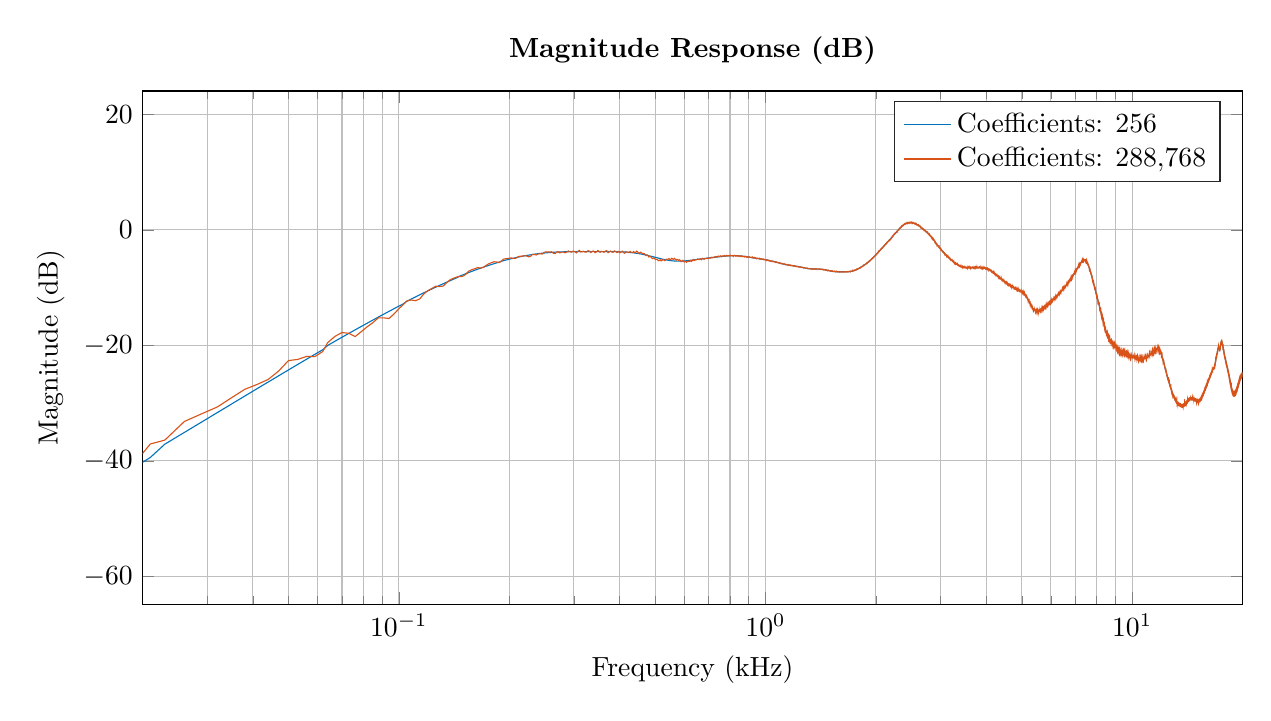
\begin{tikzpicture}

\begin{axis}[%
width=5.5in,
height=2.566in,
at={(2.804in,1.205in)},
scale only axis,
xmode=log,
xmin=0.020,
xmax=20.000,
xminorticks=true,
xlabel={Frequency (kHz)},
xmajorgrids,
xminorgrids,
ymin=-64.832,
ymax=24.080,
ylabel={Magnitude (dB)},
ymajorgrids,
axis background/.style={fill=white},
title style={font=\bfseries},
title={Magnitude Response (dB)},
legend style={legend cell align=left,align=left,draw=white!15!black}
]
\addplot [color=mycolor1,solid,forget plot]
  table[row sep=crcr]{%
0.018	-42.077\\
0.021	-39.419\\
0.023	-37.115\\
0.026	-35.084\\
0.029	-33.272\\
0.032	-31.636\\
0.035	-30.148\\
0.038	-28.784\\
0.041	-27.525\\
0.044	-26.358\\
0.047	-25.271\\
0.050	-24.254\\
0.053	-23.301\\
0.056	-22.403\\
0.059	-21.556\\
0.062	-20.755\\
0.064	-19.995\\
0.067	-19.274\\
0.070	-18.589\\
0.073	-17.935\\
0.076	-17.312\\
0.079	-16.718\\
0.082	-16.149\\
0.085	-15.605\\
0.088	-15.083\\
0.091	-14.584\\
0.094	-14.105\\
0.097	-13.645\\
0.100	-13.203\\
0.103	-12.779\\
0.105	-12.371\\
0.108	-11.979\\
0.111	-11.602\\
0.114	-11.239\\
0.117	-10.890\\
0.120	-10.554\\
0.123	-10.231\\
0.126	-9.920\\
0.129	-9.620\\
0.132	-9.332\\
0.135	-9.055\\
0.138	-8.788\\
0.141	-8.531\\
0.144	-8.284\\
0.146	-8.046\\
0.149	-7.818\\
0.152	-7.598\\
0.155	-7.387\\
0.158	-7.184\\
0.161	-6.990\\
0.164	-6.803\\
0.167	-6.624\\
0.170	-6.452\\
0.173	-6.288\\
0.176	-6.131\\
0.179	-5.980\\
0.182	-5.836\\
0.185	-5.699\\
0.188	-5.568\\
0.190	-5.443\\
0.193	-5.324\\
0.196	-5.211\\
0.199	-5.103\\
0.202	-5.001\\
0.205	-4.904\\
0.208	-4.813\\
0.211	-4.727\\
0.214	-4.645\\
0.217	-4.568\\
0.220	-4.496\\
0.223	-4.428\\
0.226	-4.365\\
0.229	-4.306\\
0.231	-4.251\\
0.234	-4.199\\
0.237	-4.152\\
0.240	-4.108\\
0.243	-4.068\\
0.246	-4.030\\
0.249	-3.996\\
0.252	-3.965\\
0.255	-3.937\\
0.258	-3.912\\
0.261	-3.889\\
0.264	-3.869\\
0.267	-3.850\\
0.270	-3.834\\
0.272	-3.820\\
0.275	-3.808\\
0.278	-3.798\\
0.281	-3.789\\
0.284	-3.781\\
0.287	-3.775\\
0.290	-3.770\\
0.293	-3.766\\
0.296	-3.763\\
0.299	-3.760\\
0.302	-3.759\\
0.305	-3.758\\
0.308	-3.757\\
0.311	-3.757\\
0.313	-3.757\\
0.316	-3.757\\
0.319	-3.757\\
0.322	-3.757\\
0.325	-3.758\\
0.328	-3.758\\
0.331	-3.758\\
0.334	-3.758\\
0.337	-3.759\\
0.340	-3.758\\
0.343	-3.758\\
0.346	-3.758\\
0.349	-3.758\\
0.352	-3.757\\
0.354	-3.757\\
0.357	-3.756\\
0.360	-3.756\\
0.363	-3.755\\
0.366	-3.755\\
0.369	-3.755\\
0.372	-3.755\\
0.375	-3.756\\
0.378	-3.757\\
0.381	-3.758\\
0.384	-3.760\\
0.387	-3.763\\
0.390	-3.767\\
0.393	-3.771\\
0.396	-3.776\\
0.398	-3.782\\
0.401	-3.789\\
0.404	-3.797\\
0.407	-3.806\\
0.410	-3.816\\
0.413	-3.827\\
0.416	-3.840\\
0.419	-3.854\\
0.422	-3.870\\
0.425	-3.886\\
0.428	-3.905\\
0.431	-3.924\\
0.434	-3.945\\
0.437	-3.968\\
0.439	-3.992\\
0.442	-4.017\\
0.445	-4.044\\
0.448	-4.072\\
0.451	-4.102\\
0.454	-4.133\\
0.457	-4.165\\
0.460	-4.198\\
0.463	-4.233\\
0.466	-4.269\\
0.469	-4.305\\
0.472	-4.343\\
0.475	-4.382\\
0.478	-4.421\\
0.480	-4.461\\
0.483	-4.502\\
0.486	-4.543\\
0.489	-4.585\\
0.492	-4.627\\
0.495	-4.668\\
0.498	-4.710\\
0.501	-4.752\\
0.504	-4.793\\
0.507	-4.834\\
0.510	-4.874\\
0.513	-4.914\\
0.516	-4.953\\
0.519	-4.991\\
0.521	-5.028\\
0.524	-5.063\\
0.527	-5.097\\
0.530	-5.130\\
0.533	-5.161\\
0.536	-5.191\\
0.539	-5.219\\
0.542	-5.245\\
0.545	-5.269\\
0.548	-5.291\\
0.551	-5.312\\
0.554	-5.330\\
0.557	-5.346\\
0.560	-5.361\\
0.562	-5.373\\
0.565	-5.383\\
0.568	-5.391\\
0.571	-5.398\\
0.574	-5.402\\
0.577	-5.405\\
0.580	-5.405\\
0.583	-5.405\\
0.586	-5.402\\
0.589	-5.398\\
0.592	-5.392\\
0.595	-5.386\\
0.598	-5.377\\
0.601	-5.368\\
0.604	-5.358\\
0.606	-5.346\\
0.609	-5.334\\
0.612	-5.321\\
0.615	-5.307\\
0.618	-5.293\\
0.621	-5.278\\
0.624	-5.263\\
0.627	-5.247\\
0.630	-5.231\\
0.633	-5.215\\
0.636	-5.199\\
0.639	-5.182\\
0.642	-5.166\\
0.645	-5.149\\
0.647	-5.133\\
0.650	-5.116\\
0.653	-5.100\\
0.656	-5.084\\
0.659	-5.068\\
0.662	-5.052\\
0.665	-5.036\\
0.668	-5.021\\
0.671	-5.005\\
0.674	-4.990\\
0.677	-4.975\\
0.680	-4.960\\
0.683	-4.946\\
0.686	-4.931\\
0.688	-4.917\\
0.691	-4.902\\
0.694	-4.888\\
0.697	-4.874\\
0.700	-4.860\\
0.703	-4.847\\
0.706	-4.833\\
0.709	-4.819\\
0.712	-4.806\\
0.715	-4.792\\
0.718	-4.778\\
0.721	-4.765\\
0.724	-4.751\\
0.727	-4.738\\
0.729	-4.725\\
0.732	-4.711\\
0.735	-4.698\\
0.738	-4.685\\
0.741	-4.672\\
0.744	-4.659\\
0.747	-4.646\\
0.750	-4.633\\
0.753	-4.621\\
0.756	-4.608\\
0.759	-4.596\\
0.762	-4.584\\
0.765	-4.573\\
0.768	-4.561\\
0.771	-4.550\\
0.773	-4.540\\
0.776	-4.530\\
0.779	-4.520\\
0.782	-4.511\\
0.785	-4.502\\
0.788	-4.494\\
0.791	-4.487\\
0.794	-4.480\\
0.797	-4.473\\
0.800	-4.468\\
0.803	-4.463\\
0.806	-4.458\\
0.809	-4.455\\
0.812	-4.452\\
0.814	-4.450\\
0.817	-4.449\\
0.820	-4.449\\
0.823	-4.449\\
0.826	-4.450\\
0.829	-4.452\\
0.832	-4.455\\
0.835	-4.459\\
0.838	-4.463\\
0.841	-4.469\\
0.844	-4.475\\
0.847	-4.481\\
0.850	-4.489\\
0.853	-4.497\\
0.855	-4.506\\
0.858	-4.516\\
0.861	-4.526\\
0.864	-4.537\\
0.867	-4.548\\
0.870	-4.560\\
0.873	-4.573\\
0.876	-4.586\\
0.879	-4.599\\
0.882	-4.613\\
0.885	-4.627\\
0.888	-4.641\\
0.891	-4.656\\
0.894	-4.671\\
0.896	-4.686\\
0.899	-4.701\\
0.902	-4.716\\
0.905	-4.732\\
0.908	-4.747\\
0.911	-4.762\\
0.914	-4.778\\
0.917	-4.793\\
0.920	-4.808\\
0.923	-4.823\\
0.926	-4.838\\
0.929	-4.852\\
0.932	-4.867\\
0.935	-4.881\\
0.938	-4.895\\
0.940	-4.909\\
0.943	-4.923\\
0.946	-4.937\\
0.949	-4.950\\
0.952	-4.963\\
0.955	-4.976\\
0.958	-4.989\\
0.961	-5.001\\
0.964	-5.014\\
0.967	-5.026\\
0.970	-5.039\\
0.973	-5.051\\
0.976	-5.063\\
0.979	-5.075\\
0.981	-5.088\\
0.984	-5.100\\
0.987	-5.112\\
0.990	-5.125\\
0.993	-5.138\\
0.996	-5.150\\
0.999	-5.164\\
1.002	-5.177\\
1.005	-5.190\\
1.008	-5.204\\
1.011	-5.219\\
1.014	-5.233\\
1.017	-5.248\\
1.020	-5.263\\
1.022	-5.279\\
1.025	-5.295\\
1.028	-5.311\\
1.031	-5.328\\
1.034	-5.345\\
1.037	-5.362\\
1.040	-5.380\\
1.043	-5.398\\
1.046	-5.417\\
1.049	-5.436\\
1.052	-5.455\\
1.055	-5.475\\
1.058	-5.494\\
1.061	-5.515\\
1.063	-5.535\\
1.066	-5.555\\
1.069	-5.576\\
1.072	-5.597\\
1.075	-5.618\\
1.078	-5.638\\
1.081	-5.659\\
1.084	-5.680\\
1.087	-5.701\\
1.090	-5.721\\
1.093	-5.742\\
1.096	-5.762\\
1.099	-5.782\\
1.102	-5.802\\
1.104	-5.821\\
1.107	-5.841\\
1.110	-5.859\\
1.113	-5.878\\
1.116	-5.896\\
1.119	-5.913\\
1.122	-5.930\\
1.125	-5.947\\
1.128	-5.963\\
1.131	-5.978\\
1.134	-5.994\\
1.137	-6.008\\
1.140	-6.022\\
1.143	-6.036\\
1.146	-6.049\\
1.148	-6.062\\
1.151	-6.074\\
1.154	-6.086\\
1.157	-6.098\\
1.160	-6.109\\
1.163	-6.120\\
1.166	-6.130\\
1.169	-6.140\\
1.172	-6.150\\
1.175	-6.160\\
1.178	-6.170\\
1.181	-6.179\\
1.184	-6.189\\
1.187	-6.198\\
1.189	-6.208\\
1.192	-6.217\\
1.195	-6.227\\
1.198	-6.236\\
1.201	-6.246\\
1.204	-6.256\\
1.207	-6.266\\
1.210	-6.276\\
1.213	-6.287\\
1.216	-6.298\\
1.219	-6.309\\
1.222	-6.320\\
1.225	-6.331\\
1.228	-6.343\\
1.230	-6.355\\
1.233	-6.368\\
1.236	-6.380\\
1.239	-6.393\\
1.242	-6.406\\
1.245	-6.420\\
1.248	-6.433\\
1.251	-6.447\\
1.254	-6.461\\
1.257	-6.475\\
1.260	-6.489\\
1.263	-6.503\\
1.266	-6.517\\
1.269	-6.531\\
1.271	-6.545\\
1.274	-6.559\\
1.277	-6.573\\
1.280	-6.587\\
1.283	-6.600\\
1.286	-6.613\\
1.289	-6.626\\
1.292	-6.638\\
1.295	-6.650\\
1.298	-6.661\\
1.301	-6.672\\
1.304	-6.683\\
1.307	-6.693\\
1.310	-6.702\\
1.312	-6.711\\
1.315	-6.720\\
1.318	-6.727\\
1.321	-6.734\\
1.324	-6.741\\
1.327	-6.747\\
1.330	-6.752\\
1.333	-6.757\\
1.336	-6.761\\
1.339	-6.765\\
1.342	-6.768\\
1.345	-6.770\\
1.348	-6.772\\
1.351	-6.774\\
1.354	-6.775\\
1.356	-6.776\\
1.359	-6.777\\
1.362	-6.777\\
1.365	-6.777\\
1.368	-6.777\\
1.371	-6.777\\
1.374	-6.777\\
1.377	-6.777\\
1.380	-6.777\\
1.383	-6.777\\
1.386	-6.777\\
1.389	-6.777\\
1.392	-6.778\\
1.395	-6.778\\
1.397	-6.780\\
1.400	-6.781\\
1.403	-6.783\\
1.406	-6.785\\
1.409	-6.788\\
1.412	-6.791\\
1.415	-6.795\\
1.418	-6.800\\
1.421	-6.804\\
1.424	-6.810\\
1.427	-6.816\\
1.430	-6.823\\
1.433	-6.830\\
1.436	-6.837\\
1.438	-6.846\\
1.441	-6.855\\
1.444	-6.864\\
1.447	-6.874\\
1.450	-6.884\\
1.453	-6.895\\
1.456	-6.906\\
1.459	-6.918\\
1.462	-6.930\\
1.465	-6.942\\
1.468	-6.955\\
1.471	-6.967\\
1.474	-6.980\\
1.477	-6.993\\
1.479	-7.006\\
1.482	-7.020\\
1.485	-7.033\\
1.488	-7.046\\
1.491	-7.059\\
1.494	-7.071\\
1.497	-7.084\\
1.500	-7.096\\
1.503	-7.108\\
1.506	-7.120\\
1.509	-7.131\\
1.512	-7.142\\
1.515	-7.153\\
1.518	-7.162\\
1.521	-7.172\\
1.523	-7.181\\
1.526	-7.189\\
1.529	-7.197\\
1.532	-7.204\\
1.535	-7.211\\
1.538	-7.217\\
1.541	-7.222\\
1.544	-7.227\\
1.547	-7.232\\
1.550	-7.236\\
1.553	-7.239\\
1.556	-7.242\\
1.559	-7.244\\
1.562	-7.246\\
1.564	-7.248\\
1.567	-7.249\\
1.570	-7.250\\
1.573	-7.251\\
1.576	-7.251\\
1.579	-7.251\\
1.582	-7.251\\
1.585	-7.250\\
1.588	-7.250\\
1.591	-7.249\\
1.594	-7.248\\
1.597	-7.247\\
1.600	-7.247\\
1.603	-7.246\\
1.605	-7.245\\
1.608	-7.244\\
1.611	-7.244\\
1.614	-7.243\\
1.617	-7.243\\
1.620	-7.242\\
1.623	-7.242\\
1.626	-7.242\\
1.629	-7.242\\
1.632	-7.242\\
1.635	-7.242\\
1.638	-7.242\\
1.641	-7.243\\
1.644	-7.243\\
1.646	-7.243\\
1.649	-7.244\\
1.652	-7.244\\
1.655	-7.244\\
1.658	-7.245\\
1.661	-7.245\\
1.664	-7.245\\
1.667	-7.244\\
1.670	-7.244\\
1.673	-7.243\\
1.676	-7.242\\
1.679	-7.240\\
1.682	-7.238\\
1.685	-7.236\\
1.688	-7.233\\
1.690	-7.230\\
1.693	-7.226\\
1.696	-7.221\\
1.699	-7.216\\
1.702	-7.210\\
1.705	-7.204\\
1.708	-7.196\\
1.711	-7.188\\
1.714	-7.180\\
1.717	-7.170\\
1.720	-7.160\\
1.723	-7.149\\
1.726	-7.137\\
1.729	-7.125\\
1.731	-7.111\\
1.734	-7.097\\
1.737	-7.082\\
1.740	-7.067\\
1.743	-7.050\\
1.746	-7.033\\
1.749	-7.016\\
1.752	-6.997\\
1.755	-6.978\\
1.758	-6.959\\
1.761	-6.938\\
1.764	-6.917\\
1.767	-6.896\\
1.770	-6.874\\
1.772	-6.852\\
1.775	-6.829\\
1.778	-6.806\\
1.781	-6.783\\
1.784	-6.759\\
1.787	-6.735\\
1.790	-6.711\\
1.793	-6.686\\
1.796	-6.661\\
1.799	-6.636\\
1.802	-6.611\\
1.805	-6.586\\
1.808	-6.560\\
1.811	-6.534\\
1.813	-6.509\\
1.816	-6.483\\
1.819	-6.457\\
1.822	-6.431\\
1.825	-6.404\\
1.828	-6.378\\
1.831	-6.352\\
1.834	-6.325\\
1.837	-6.298\\
1.840	-6.271\\
1.843	-6.244\\
1.846	-6.217\\
1.849	-6.190\\
1.852	-6.162\\
1.854	-6.135\\
1.857	-6.107\\
1.860	-6.078\\
1.863	-6.050\\
1.866	-6.021\\
1.869	-5.992\\
1.872	-5.963\\
1.875	-5.933\\
1.878	-5.903\\
1.881	-5.872\\
1.884	-5.841\\
1.887	-5.810\\
1.890	-5.778\\
1.893	-5.746\\
1.896	-5.713\\
1.898	-5.680\\
1.901	-5.647\\
1.904	-5.613\\
1.907	-5.578\\
1.910	-5.543\\
1.913	-5.508\\
1.916	-5.472\\
1.919	-5.435\\
1.922	-5.398\\
1.925	-5.361\\
1.928	-5.323\\
1.931	-5.285\\
1.934	-5.246\\
1.937	-5.207\\
1.939	-5.168\\
1.942	-5.128\\
1.945	-5.088\\
1.948	-5.047\\
1.951	-5.006\\
1.954	-4.965\\
1.957	-4.924\\
1.960	-4.882\\
1.963	-4.840\\
1.966	-4.798\\
1.969	-4.755\\
1.972	-4.713\\
1.975	-4.670\\
1.978	-4.627\\
1.980	-4.584\\
1.983	-4.541\\
1.986	-4.498\\
1.989	-4.455\\
1.992	-4.411\\
1.995	-4.368\\
1.998	-4.325\\
2.001	-4.281\\
2.004	-4.238\\
2.007	-4.195\\
2.010	-4.151\\
2.013	-4.108\\
2.016	-4.065\\
2.019	-4.021\\
2.021	-3.978\\
2.024	-3.935\\
2.027	-3.892\\
2.030	-3.849\\
2.033	-3.807\\
2.036	-3.764\\
2.039	-3.721\\
2.042	-3.678\\
2.045	-3.636\\
2.048	-3.593\\
2.051	-3.551\\
2.054	-3.509\\
2.057	-3.466\\
2.060	-3.424\\
2.062	-3.382\\
2.065	-3.340\\
2.068	-3.298\\
2.071	-3.256\\
2.074	-3.214\\
2.077	-3.172\\
2.080	-3.130\\
2.083	-3.088\\
2.086	-3.047\\
2.089	-3.005\\
2.092	-2.963\\
2.095	-2.921\\
2.098	-2.880\\
2.101	-2.838\\
2.104	-2.796\\
2.106	-2.755\\
2.109	-2.713\\
2.112	-2.672\\
2.115	-2.630\\
2.118	-2.588\\
2.121	-2.547\\
2.124	-2.505\\
2.127	-2.464\\
2.130	-2.422\\
2.133	-2.381\\
2.136	-2.339\\
2.139	-2.298\\
2.142	-2.256\\
2.145	-2.215\\
2.147	-2.174\\
2.150	-2.132\\
2.153	-2.091\\
2.156	-2.049\\
2.159	-2.008\\
2.162	-1.967\\
2.165	-1.925\\
2.168	-1.884\\
2.171	-1.843\\
2.174	-1.801\\
2.177	-1.760\\
2.180	-1.718\\
2.183	-1.677\\
2.186	-1.636\\
2.188	-1.594\\
2.191	-1.553\\
2.194	-1.512\\
2.197	-1.470\\
2.200	-1.429\\
2.203	-1.388\\
2.206	-1.346\\
2.209	-1.305\\
2.212	-1.263\\
2.215	-1.222\\
2.218	-1.181\\
2.221	-1.139\\
2.224	-1.098\\
2.227	-1.056\\
2.229	-1.015\\
2.232	-0.973\\
2.235	-0.932\\
2.238	-0.890\\
2.241	-0.848\\
2.244	-0.807\\
2.247	-0.765\\
2.250	-0.724\\
2.253	-0.682\\
2.256	-0.641\\
2.259	-0.599\\
2.262	-0.558\\
2.265	-0.517\\
2.268	-0.476\\
2.271	-0.434\\
2.273	-0.393\\
2.276	-0.352\\
2.279	-0.312\\
2.282	-0.271\\
2.285	-0.230\\
2.288	-0.190\\
2.291	-0.150\\
2.294	-0.110\\
2.297	-0.070\\
2.300	-0.031\\
2.303	0.009\\
2.306	0.047\\
2.309	0.086\\
2.312	0.124\\
2.314	0.162\\
2.317	0.200\\
2.320	0.237\\
2.323	0.274\\
2.326	0.310\\
2.329	0.346\\
2.332	0.381\\
2.335	0.416\\
2.338	0.450\\
2.341	0.484\\
2.344	0.517\\
2.347	0.550\\
2.350	0.582\\
2.353	0.613\\
2.355	0.644\\
2.358	0.674\\
2.361	0.704\\
2.364	0.733\\
2.367	0.761\\
2.370	0.788\\
2.373	0.815\\
2.376	0.841\\
2.379	0.867\\
2.382	0.891\\
2.385	0.915\\
2.388	0.938\\
2.391	0.960\\
2.394	0.982\\
2.396	1.002\\
2.399	1.022\\
2.402	1.042\\
2.405	1.060\\
2.408	1.077\\
2.411	1.094\\
2.414	1.110\\
2.417	1.126\\
2.420	1.140\\
2.423	1.154\\
2.426	1.167\\
2.429	1.179\\
2.432	1.190\\
2.435	1.201\\
2.438	1.211\\
2.440	1.220\\
2.443	1.228\\
2.446	1.236\\
2.449	1.243\\
2.452	1.249\\
2.455	1.255\\
2.458	1.260\\
2.461	1.264\\
2.464	1.268\\
2.467	1.270\\
2.470	1.273\\
2.473	1.274\\
2.476	1.275\\
2.479	1.276\\
2.481	1.275\\
2.484	1.275\\
2.487	1.273\\
2.490	1.271\\
2.493	1.269\\
2.496	1.266\\
2.499	1.262\\
2.502	1.258\\
2.505	1.253\\
2.508	1.248\\
2.511	1.242\\
2.514	1.236\\
2.517	1.229\\
2.520	1.222\\
2.522	1.214\\
2.525	1.206\\
2.528	1.198\\
2.531	1.189\\
2.534	1.179\\
2.537	1.169\\
2.540	1.159\\
2.543	1.148\\
2.546	1.136\\
2.549	1.125\\
2.552	1.113\\
2.555	1.100\\
2.558	1.087\\
2.561	1.074\\
2.563	1.060\\
2.566	1.046\\
2.569	1.031\\
2.572	1.016\\
2.575	1.001\\
2.578	0.985\\
2.581	0.969\\
2.584	0.952\\
2.587	0.936\\
2.590	0.918\\
2.593	0.901\\
2.596	0.883\\
2.599	0.864\\
2.602	0.846\\
2.604	0.827\\
2.607	0.807\\
2.610	0.788\\
2.613	0.768\\
2.616	0.747\\
2.619	0.727\\
2.622	0.706\\
2.625	0.685\\
2.628	0.663\\
2.631	0.641\\
2.634	0.620\\
2.637	0.597\\
2.640	0.575\\
2.643	0.552\\
2.646	0.529\\
2.648	0.506\\
2.651	0.483\\
2.654	0.459\\
2.657	0.436\\
2.660	0.412\\
2.663	0.388\\
2.666	0.364\\
2.669	0.340\\
2.672	0.315\\
2.675	0.291\\
2.678	0.266\\
2.681	0.242\\
2.684	0.217\\
2.687	0.192\\
2.689	0.167\\
2.692	0.142\\
2.695	0.117\\
2.698	0.092\\
2.701	0.067\\
2.704	0.041\\
2.707	0.016\\
2.710	-0.009\\
2.713	-0.035\\
2.716	-0.060\\
2.719	-0.086\\
2.722	-0.111\\
2.725	-0.137\\
2.728	-0.163\\
2.730	-0.189\\
2.733	-0.214\\
2.736	-0.240\\
2.739	-0.266\\
2.742	-0.293\\
2.745	-0.319\\
2.748	-0.345\\
2.751	-0.372\\
2.754	-0.398\\
2.757	-0.425\\
2.760	-0.452\\
2.763	-0.479\\
2.766	-0.507\\
2.769	-0.534\\
2.771	-0.562\\
2.774	-0.590\\
2.777	-0.618\\
2.780	-0.647\\
2.783	-0.675\\
2.786	-0.704\\
2.789	-0.734\\
2.792	-0.763\\
2.795	-0.793\\
2.798	-0.823\\
2.801	-0.854\\
2.804	-0.884\\
2.807	-0.916\\
2.810	-0.947\\
2.812	-0.979\\
2.815	-1.011\\
2.818	-1.043\\
2.821	-1.076\\
2.824	-1.109\\
2.827	-1.143\\
2.830	-1.177\\
2.833	-1.211\\
2.836	-1.245\\
2.839	-1.280\\
2.842	-1.315\\
2.845	-1.351\\
2.848	-1.387\\
2.851	-1.423\\
2.854	-1.459\\
2.856	-1.496\\
2.859	-1.533\\
2.862	-1.570\\
2.865	-1.607\\
2.868	-1.644\\
2.871	-1.682\\
2.874	-1.720\\
2.877	-1.758\\
2.880	-1.796\\
2.883	-1.835\\
2.886	-1.873\\
2.889	-1.911\\
2.892	-1.950\\
2.895	-1.989\\
2.897	-2.027\\
2.900	-2.066\\
2.903	-2.104\\
2.906	-2.143\\
2.909	-2.181\\
2.912	-2.220\\
2.915	-2.258\\
2.918	-2.296\\
2.921	-2.334\\
2.924	-2.372\\
2.927	-2.410\\
2.930	-2.447\\
2.933	-2.485\\
2.936	-2.522\\
2.938	-2.559\\
2.941	-2.595\\
2.944	-2.632\\
2.947	-2.668\\
2.950	-2.704\\
2.953	-2.740\\
2.956	-2.776\\
2.959	-2.811\\
2.962	-2.846\\
2.965	-2.881\\
2.968	-2.915\\
2.971	-2.950\\
2.974	-2.984\\
2.977	-3.018\\
2.979	-3.051\\
2.982	-3.085\\
2.985	-3.118\\
2.988	-3.151\\
2.991	-3.184\\
2.994	-3.216\\
2.997	-3.248\\
3.000	-3.281\\
3.003	-3.313\\
3.006	-3.344\\
3.009	-3.376\\
3.012	-3.407\\
3.015	-3.439\\
3.018	-3.470\\
3.021	-3.501\\
3.023	-3.531\\
3.026	-3.562\\
3.029	-3.593\\
3.032	-3.623\\
3.035	-3.653\\
3.038	-3.684\\
3.041	-3.714\\
3.044	-3.744\\
3.047	-3.773\\
3.050	-3.803\\
3.053	-3.833\\
3.056	-3.862\\
3.059	-3.891\\
3.062	-3.921\\
3.064	-3.950\\
3.067	-3.979\\
3.070	-4.007\\
3.073	-4.036\\
3.076	-4.064\\
3.079	-4.093\\
3.082	-4.121\\
3.085	-4.149\\
3.088	-4.177\\
3.091	-4.204\\
3.094	-4.232\\
3.097	-4.259\\
3.100	-4.286\\
3.103	-4.313\\
3.105	-4.340\\
3.108	-4.366\\
3.111	-4.392\\
3.114	-4.418\\
3.117	-4.444\\
3.120	-4.470\\
3.123	-4.495\\
3.126	-4.521\\
3.129	-4.546\\
3.132	-4.570\\
3.135	-4.595\\
3.138	-4.619\\
3.141	-4.644\\
3.144	-4.668\\
3.146	-4.691\\
3.149	-4.715\\
3.152	-4.739\\
3.155	-4.762\\
3.158	-4.785\\
3.161	-4.808\\
3.164	-4.831\\
3.167	-4.853\\
3.170	-4.876\\
3.173	-4.898\\
3.176	-4.921\\
3.179	-4.943\\
3.182	-4.965\\
3.185	-4.987\\
3.188	-5.009\\
3.190	-5.030\\
3.193	-5.052\\
3.196	-5.074\\
3.199	-5.096\\
3.202	-5.117\\
3.205	-5.139\\
3.208	-5.160\\
3.211	-5.182\\
3.214	-5.203\\
3.217	-5.224\\
3.220	-5.246\\
3.223	-5.267\\
3.226	-5.288\\
3.229	-5.309\\
3.231	-5.330\\
3.234	-5.352\\
3.237	-5.373\\
3.240	-5.394\\
3.243	-5.415\\
3.246	-5.435\\
3.249	-5.456\\
3.252	-5.477\\
3.255	-5.497\\
3.258	-5.518\\
3.261	-5.538\\
3.264	-5.558\\
3.267	-5.579\\
3.270	-5.599\\
3.272	-5.618\\
3.275	-5.638\\
3.278	-5.657\\
3.281	-5.677\\
3.284	-5.696\\
3.287	-5.715\\
3.290	-5.733\\
3.293	-5.752\\
3.296	-5.770\\
3.299	-5.788\\
3.302	-5.805\\
3.305	-5.823\\
3.308	-5.840\\
3.311	-5.857\\
3.313	-5.873\\
3.316	-5.890\\
3.319	-5.906\\
3.322	-5.921\\
3.325	-5.937\\
3.328	-5.952\\
3.331	-5.967\\
3.334	-5.982\\
3.337	-5.996\\
3.340	-6.010\\
3.343	-6.024\\
3.346	-6.038\\
3.349	-6.051\\
3.352	-6.064\\
3.354	-6.077\\
3.357	-6.090\\
3.360	-6.102\\
3.363	-6.114\\
3.366	-6.126\\
3.369	-6.138\\
3.372	-6.149\\
3.375	-6.161\\
3.378	-6.172\\
3.381	-6.183\\
3.384	-6.194\\
3.387	-6.205\\
3.390	-6.215\\
3.393	-6.225\\
3.396	-6.236\\
3.398	-6.246\\
3.401	-6.256\\
3.404	-6.266\\
3.407	-6.275\\
3.410	-6.285\\
3.413	-6.295\\
3.416	-6.304\\
3.419	-6.313\\
3.422	-6.322\\
3.425	-6.331\\
3.428	-6.340\\
3.431	-6.349\\
3.434	-6.357\\
3.437	-6.365\\
3.439	-6.374\\
3.442	-6.382\\
3.445	-6.390\\
3.448	-6.397\\
3.451	-6.405\\
3.454	-6.412\\
3.457	-6.419\\
3.460	-6.426\\
3.463	-6.433\\
3.466	-6.440\\
3.469	-6.446\\
3.472	-6.452\\
3.475	-6.458\\
3.478	-6.463\\
3.480	-6.469\\
3.483	-6.474\\
3.486	-6.479\\
3.489	-6.483\\
3.492	-6.488\\
3.495	-6.492\\
3.498	-6.495\\
3.501	-6.499\\
3.504	-6.502\\
3.507	-6.505\\
3.510	-6.508\\
3.513	-6.511\\
3.516	-6.513\\
3.519	-6.515\\
3.521	-6.517\\
3.524	-6.519\\
3.527	-6.521\\
3.530	-6.522\\
3.533	-6.523\\
3.536	-6.524\\
3.539	-6.525\\
3.542	-6.525\\
3.545	-6.526\\
3.548	-6.526\\
3.551	-6.527\\
3.554	-6.527\\
3.557	-6.527\\
3.560	-6.527\\
3.562	-6.527\\
3.565	-6.527\\
3.568	-6.526\\
3.571	-6.526\\
3.574	-6.526\\
3.577	-6.526\\
3.580	-6.526\\
3.583	-6.525\\
3.586	-6.525\\
3.589	-6.525\\
3.592	-6.525\\
3.595	-6.525\\
3.598	-6.525\\
3.601	-6.525\\
3.604	-6.525\\
3.606	-6.525\\
3.609	-6.525\\
3.612	-6.525\\
3.615	-6.525\\
3.618	-6.525\\
3.621	-6.525\\
3.624	-6.526\\
3.627	-6.526\\
3.630	-6.526\\
3.633	-6.527\\
3.636	-6.527\\
3.639	-6.527\\
3.642	-6.528\\
3.645	-6.528\\
3.647	-6.529\\
3.650	-6.529\\
3.653	-6.529\\
3.656	-6.529\\
3.659	-6.530\\
3.662	-6.530\\
3.665	-6.530\\
3.668	-6.530\\
3.671	-6.530\\
3.674	-6.530\\
3.677	-6.530\\
3.680	-6.530\\
3.683	-6.529\\
3.686	-6.529\\
3.688	-6.528\\
3.691	-6.528\\
3.694	-6.527\\
3.697	-6.526\\
3.700	-6.526\\
3.703	-6.525\\
3.706	-6.524\\
3.709	-6.522\\
3.712	-6.521\\
3.715	-6.520\\
3.718	-6.519\\
3.721	-6.517\\
3.724	-6.516\\
3.727	-6.515\\
3.729	-6.513\\
3.732	-6.512\\
3.735	-6.510\\
3.738	-6.509\\
3.741	-6.507\\
3.744	-6.506\\
3.747	-6.504\\
3.750	-6.503\\
3.753	-6.501\\
3.756	-6.500\\
3.759	-6.498\\
3.762	-6.497\\
3.765	-6.496\\
3.768	-6.495\\
3.771	-6.494\\
3.773	-6.493\\
3.776	-6.492\\
3.779	-6.492\\
3.782	-6.491\\
3.785	-6.491\\
3.788	-6.490\\
3.791	-6.490\\
3.794	-6.490\\
3.797	-6.490\\
3.800	-6.490\\
3.803	-6.491\\
3.806	-6.491\\
3.809	-6.492\\
3.812	-6.492\\
3.814	-6.493\\
3.817	-6.494\\
3.820	-6.495\\
3.823	-6.497\\
3.826	-6.498\\
3.829	-6.499\\
3.832	-6.501\\
3.835	-6.502\\
3.838	-6.504\\
3.841	-6.506\\
3.844	-6.507\\
3.847	-6.509\\
3.850	-6.511\\
3.853	-6.513\\
3.855	-6.515\\
3.858	-6.517\\
3.861	-6.519\\
3.864	-6.521\\
3.867	-6.523\\
3.870	-6.526\\
3.873	-6.528\\
3.876	-6.530\\
3.879	-6.532\\
3.882	-6.534\\
3.885	-6.536\\
3.888	-6.538\\
3.891	-6.541\\
3.894	-6.543\\
3.896	-6.545\\
3.899	-6.547\\
3.902	-6.549\\
3.905	-6.551\\
3.908	-6.554\\
3.911	-6.556\\
3.914	-6.558\\
3.917	-6.560\\
3.920	-6.563\\
3.923	-6.565\\
3.926	-6.568\\
3.929	-6.570\\
3.932	-6.573\\
3.935	-6.576\\
3.938	-6.578\\
3.940	-6.581\\
3.943	-6.584\\
3.946	-6.588\\
3.949	-6.591\\
3.952	-6.594\\
3.955	-6.598\\
3.958	-6.602\\
3.961	-6.606\\
3.964	-6.610\\
3.967	-6.614\\
3.970	-6.619\\
3.973	-6.624\\
3.976	-6.629\\
3.979	-6.634\\
3.981	-6.639\\
3.984	-6.645\\
3.987	-6.651\\
3.990	-6.657\\
3.993	-6.663\\
3.996	-6.670\\
3.999	-6.677\\
4.002	-6.684\\
4.005	-6.691\\
4.008	-6.698\\
4.011	-6.706\\
4.014	-6.714\\
4.017	-6.722\\
4.020	-6.730\\
4.022	-6.739\\
4.025	-6.747\\
4.028	-6.756\\
4.031	-6.765\\
4.034	-6.775\\
4.037	-6.784\\
4.040	-6.793\\
4.043	-6.803\\
4.046	-6.813\\
4.049	-6.823\\
4.052	-6.833\\
4.055	-6.843\\
4.058	-6.853\\
4.061	-6.864\\
4.063	-6.874\\
4.066	-6.885\\
4.069	-6.895\\
4.072	-6.906\\
4.075	-6.917\\
4.078	-6.928\\
4.081	-6.939\\
4.084	-6.950\\
4.087	-6.961\\
4.090	-6.972\\
4.093	-6.983\\
4.096	-6.994\\
4.099	-7.005\\
4.102	-7.016\\
4.104	-7.028\\
4.107	-7.039\\
4.110	-7.051\\
4.113	-7.062\\
4.116	-7.074\\
4.119	-7.085\\
4.122	-7.097\\
4.125	-7.109\\
4.128	-7.121\\
4.131	-7.133\\
4.134	-7.145\\
4.137	-7.157\\
4.140	-7.170\\
4.143	-7.182\\
4.146	-7.195\\
4.148	-7.208\\
4.151	-7.221\\
4.154	-7.234\\
4.157	-7.247\\
4.160	-7.261\\
4.163	-7.275\\
4.166	-7.288\\
4.169	-7.302\\
4.172	-7.317\\
4.175	-7.331\\
4.178	-7.346\\
4.181	-7.360\\
4.184	-7.375\\
4.187	-7.390\\
4.189	-7.406\\
4.192	-7.421\\
4.195	-7.437\\
4.198	-7.453\\
4.201	-7.469\\
4.204	-7.485\\
4.207	-7.501\\
4.210	-7.518\\
4.213	-7.534\\
4.216	-7.551\\
4.219	-7.568\\
4.222	-7.584\\
4.225	-7.601\\
4.228	-7.618\\
4.230	-7.636\\
4.233	-7.653\\
4.236	-7.670\\
4.239	-7.687\\
4.242	-7.704\\
4.245	-7.721\\
4.248	-7.738\\
4.251	-7.755\\
4.254	-7.772\\
4.257	-7.789\\
4.260	-7.806\\
4.263	-7.823\\
4.266	-7.840\\
4.269	-7.856\\
4.271	-7.873\\
4.274	-7.889\\
4.277	-7.905\\
4.280	-7.921\\
4.283	-7.937\\
4.286	-7.953\\
4.289	-7.969\\
4.292	-7.984\\
4.295	-8.000\\
4.298	-8.015\\
4.301	-8.030\\
4.304	-8.045\\
4.307	-8.060\\
4.310	-8.074\\
4.312	-8.089\\
4.315	-8.103\\
4.318	-8.117\\
4.321	-8.132\\
4.324	-8.146\\
4.327	-8.160\\
4.330	-8.174\\
4.333	-8.188\\
4.336	-8.202\\
4.339	-8.216\\
4.342	-8.229\\
4.345	-8.243\\
4.348	-8.257\\
4.351	-8.271\\
4.354	-8.285\\
4.356	-8.299\\
4.359	-8.313\\
4.362	-8.327\\
4.365	-8.341\\
4.368	-8.355\\
4.371	-8.369\\
4.374	-8.384\\
4.377	-8.398\\
4.380	-8.413\\
4.383	-8.427\\
4.386	-8.442\\
4.389	-8.457\\
4.392	-8.472\\
4.395	-8.487\\
4.397	-8.502\\
4.400	-8.517\\
4.403	-8.532\\
4.406	-8.548\\
4.409	-8.563\\
4.412	-8.579\\
4.415	-8.595\\
4.418	-8.610\\
4.421	-8.626\\
4.424	-8.642\\
4.427	-8.658\\
4.430	-8.673\\
4.433	-8.689\\
4.436	-8.705\\
4.438	-8.721\\
4.441	-8.736\\
4.444	-8.752\\
4.447	-8.767\\
4.450	-8.783\\
4.453	-8.798\\
4.456	-8.813\\
4.459	-8.829\\
4.462	-8.844\\
4.465	-8.858\\
4.468	-8.873\\
4.471	-8.888\\
4.474	-8.902\\
4.477	-8.916\\
4.479	-8.930\\
4.482	-8.944\\
4.485	-8.958\\
4.488	-8.971\\
4.491	-8.985\\
4.494	-8.998\\
4.497	-9.011\\
4.500	-9.023\\
4.503	-9.036\\
4.506	-9.048\\
4.509	-9.061\\
4.512	-9.073\\
4.515	-9.085\\
4.518	-9.097\\
4.521	-9.108\\
4.523	-9.120\\
4.526	-9.131\\
4.529	-9.143\\
4.532	-9.154\\
4.535	-9.165\\
4.538	-9.177\\
4.541	-9.188\\
4.544	-9.199\\
4.547	-9.210\\
4.550	-9.221\\
4.553	-9.233\\
4.556	-9.244\\
4.559	-9.255\\
4.562	-9.266\\
4.564	-9.278\\
4.567	-9.289\\
4.570	-9.300\\
4.573	-9.312\\
4.576	-9.324\\
4.579	-9.335\\
4.582	-9.347\\
4.585	-9.359\\
4.588	-9.371\\
4.591	-9.383\\
4.594	-9.395\\
4.597	-9.407\\
4.600	-9.420\\
4.603	-9.432\\
4.605	-9.444\\
4.608	-9.457\\
4.611	-9.470\\
4.614	-9.482\\
4.617	-9.495\\
4.620	-9.507\\
4.623	-9.520\\
4.626	-9.533\\
4.629	-9.545\\
4.632	-9.558\\
4.635	-9.571\\
4.638	-9.583\\
4.641	-9.596\\
4.644	-9.608\\
4.646	-9.620\\
4.649	-9.633\\
4.652	-9.645\\
4.655	-9.657\\
4.658	-9.669\\
4.661	-9.680\\
4.664	-9.692\\
4.667	-9.703\\
4.670	-9.715\\
4.673	-9.726\\
4.676	-9.737\\
4.679	-9.747\\
4.682	-9.758\\
4.685	-9.768\\
4.688	-9.778\\
4.690	-9.788\\
4.693	-9.798\\
4.696	-9.808\\
4.699	-9.817\\
4.702	-9.827\\
4.705	-9.836\\
4.708	-9.845\\
4.711	-9.854\\
4.714	-9.863\\
4.717	-9.871\\
4.720	-9.880\\
4.723	-9.888\\
4.726	-9.897\\
4.729	-9.905\\
4.731	-9.913\\
4.734	-9.921\\
4.737	-9.929\\
4.740	-9.938\\
4.743	-9.946\\
4.746	-9.954\\
4.749	-9.962\\
4.752	-9.970\\
4.755	-9.978\\
4.758	-9.987\\
4.761	-9.995\\
4.764	-10.003\\
4.767	-10.012\\
4.770	-10.020\\
4.772	-10.029\\
4.775	-10.037\\
4.778	-10.046\\
4.781	-10.055\\
4.784	-10.064\\
4.787	-10.073\\
4.790	-10.082\\
4.793	-10.091\\
4.796	-10.100\\
4.799	-10.110\\
4.802	-10.119\\
4.805	-10.128\\
4.808	-10.138\\
4.811	-10.147\\
4.813	-10.157\\
4.816	-10.166\\
4.819	-10.176\\
4.822	-10.185\\
4.825	-10.195\\
4.828	-10.204\\
4.831	-10.214\\
4.834	-10.223\\
4.837	-10.232\\
4.840	-10.242\\
4.843	-10.251\\
4.846	-10.260\\
4.849	-10.269\\
4.852	-10.278\\
4.854	-10.286\\
4.857	-10.295\\
4.860	-10.304\\
4.863	-10.312\\
4.866	-10.320\\
4.869	-10.328\\
4.872	-10.336\\
4.875	-10.344\\
4.878	-10.352\\
4.881	-10.360\\
4.884	-10.367\\
4.887	-10.374\\
4.890	-10.382\\
4.893	-10.389\\
4.896	-10.396\\
4.898	-10.403\\
4.901	-10.410\\
4.904	-10.416\\
4.907	-10.423\\
4.910	-10.430\\
4.913	-10.437\\
4.916	-10.443\\
4.919	-10.450\\
4.922	-10.457\\
4.925	-10.464\\
4.928	-10.471\\
4.931	-10.477\\
4.934	-10.484\\
4.937	-10.492\\
4.939	-10.499\\
4.942	-10.506\\
4.945	-10.514\\
4.948	-10.521\\
4.951	-10.529\\
4.954	-10.537\\
4.957	-10.546\\
4.960	-10.554\\
4.963	-10.563\\
4.966	-10.572\\
4.969	-10.581\\
4.972	-10.590\\
4.975	-10.600\\
4.978	-10.610\\
4.980	-10.620\\
4.983	-10.630\\
4.986	-10.641\\
4.989	-10.652\\
4.992	-10.663\\
4.995	-10.675\\
4.998	-10.686\\
5.001	-10.698\\
5.004	-10.711\\
5.007	-10.723\\
5.010	-10.736\\
5.013	-10.749\\
5.016	-10.762\\
5.019	-10.775\\
5.021	-10.789\\
5.024	-10.803\\
5.027	-10.817\\
5.030	-10.831\\
5.033	-10.845\\
5.036	-10.860\\
5.039	-10.874\\
5.042	-10.889\\
5.045	-10.904\\
5.048	-10.919\\
5.051	-10.935\\
5.054	-10.950\\
5.057	-10.965\\
5.060	-10.981\\
5.062	-10.997\\
5.065	-11.013\\
5.068	-11.029\\
5.071	-11.045\\
5.074	-11.062\\
5.077	-11.078\\
5.080	-11.095\\
5.083	-11.111\\
5.086	-11.128\\
5.089	-11.146\\
5.092	-11.163\\
5.095	-11.180\\
5.098	-11.198\\
5.101	-11.216\\
5.104	-11.234\\
5.106	-11.253\\
5.109	-11.271\\
5.112	-11.290\\
5.115	-11.309\\
5.118	-11.329\\
5.121	-11.349\\
5.124	-11.369\\
5.127	-11.390\\
5.130	-11.410\\
5.133	-11.432\\
5.136	-11.453\\
5.139	-11.475\\
5.142	-11.498\\
5.145	-11.521\\
5.147	-11.544\\
5.150	-11.568\\
5.153	-11.592\\
5.156	-11.616\\
5.159	-11.641\\
5.162	-11.667\\
5.165	-11.693\\
5.168	-11.719\\
5.171	-11.746\\
5.174	-11.773\\
5.177	-11.801\\
5.180	-11.829\\
5.183	-11.858\\
5.186	-11.887\\
5.188	-11.916\\
5.191	-11.946\\
5.194	-11.976\\
5.197	-12.007\\
5.200	-12.038\\
5.203	-12.069\\
5.206	-12.100\\
5.209	-12.132\\
5.212	-12.164\\
5.215	-12.196\\
5.218	-12.228\\
5.221	-12.261\\
5.224	-12.294\\
5.227	-12.326\\
5.229	-12.359\\
5.232	-12.392\\
5.235	-12.425\\
5.238	-12.458\\
5.241	-12.491\\
5.244	-12.524\\
5.247	-12.556\\
5.250	-12.589\\
5.253	-12.621\\
5.256	-12.653\\
5.259	-12.685\\
5.262	-12.717\\
5.265	-12.749\\
5.268	-12.780\\
5.271	-12.811\\
5.273	-12.842\\
5.276	-12.872\\
5.279	-12.902\\
5.282	-12.932\\
5.285	-12.961\\
5.288	-12.990\\
5.291	-13.018\\
5.294	-13.047\\
5.297	-13.074\\
5.300	-13.102\\
5.303	-13.129\\
5.306	-13.155\\
5.309	-13.182\\
5.312	-13.208\\
5.314	-13.233\\
5.317	-13.258\\
5.320	-13.283\\
5.323	-13.307\\
5.326	-13.331\\
5.329	-13.355\\
5.332	-13.379\\
5.335	-13.402\\
5.338	-13.424\\
5.341	-13.447\\
5.344	-13.469\\
5.347	-13.491\\
5.350	-13.512\\
5.353	-13.534\\
5.355	-13.554\\
5.358	-13.575\\
5.361	-13.596\\
5.364	-13.616\\
5.367	-13.635\\
5.370	-13.655\\
5.373	-13.674\\
5.376	-13.693\\
5.379	-13.712\\
5.382	-13.730\\
5.385	-13.748\\
5.388	-13.766\\
5.391	-13.783\\
5.394	-13.800\\
5.396	-13.816\\
5.399	-13.832\\
5.402	-13.848\\
5.405	-13.863\\
5.408	-13.878\\
5.411	-13.893\\
5.414	-13.907\\
5.417	-13.920\\
5.420	-13.933\\
5.423	-13.946\\
5.426	-13.958\\
5.429	-13.969\\
5.432	-13.980\\
5.435	-13.990\\
5.438	-14.000\\
5.440	-14.010\\
5.443	-14.018\\
5.446	-14.026\\
5.449	-14.034\\
5.452	-14.041\\
5.455	-14.047\\
5.458	-14.053\\
5.461	-14.058\\
5.464	-14.063\\
5.467	-14.067\\
5.470	-14.071\\
5.473	-14.074\\
5.476	-14.077\\
5.479	-14.079\\
5.481	-14.080\\
5.484	-14.082\\
5.487	-14.082\\
5.490	-14.083\\
5.493	-14.083\\
5.496	-14.083\\
5.499	-14.082\\
5.502	-14.081\\
5.505	-14.080\\
5.508	-14.078\\
5.511	-14.076\\
5.514	-14.074\\
5.517	-14.072\\
5.520	-14.070\\
5.522	-14.068\\
5.525	-14.065\\
5.528	-14.062\\
5.531	-14.059\\
5.534	-14.057\\
5.537	-14.054\\
5.540	-14.051\\
5.543	-14.047\\
5.546	-14.044\\
5.549	-14.041\\
5.552	-14.038\\
5.555	-14.035\\
5.558	-14.032\\
5.561	-14.028\\
5.563	-14.025\\
5.566	-14.022\\
5.569	-14.018\\
5.572	-14.015\\
5.575	-14.012\\
5.578	-14.008\\
5.581	-14.004\\
5.584	-14.001\\
5.587	-13.997\\
5.590	-13.993\\
5.593	-13.989\\
5.596	-13.985\\
5.599	-13.980\\
5.602	-13.976\\
5.604	-13.971\\
5.607	-13.966\\
5.610	-13.961\\
5.613	-13.955\\
5.616	-13.950\\
5.619	-13.944\\
5.622	-13.937\\
5.625	-13.931\\
5.628	-13.924\\
5.631	-13.917\\
5.634	-13.910\\
5.637	-13.902\\
5.640	-13.894\\
5.643	-13.886\\
5.646	-13.877\\
5.648	-13.868\\
5.651	-13.859\\
5.654	-13.849\\
5.657	-13.839\\
5.660	-13.829\\
5.663	-13.819\\
5.666	-13.808\\
5.669	-13.798\\
5.672	-13.787\\
5.675	-13.776\\
5.678	-13.764\\
5.681	-13.753\\
5.684	-13.741\\
5.687	-13.729\\
5.689	-13.717\\
5.692	-13.705\\
5.695	-13.693\\
5.698	-13.681\\
5.701	-13.669\\
5.704	-13.657\\
5.707	-13.645\\
5.710	-13.633\\
5.713	-13.621\\
5.716	-13.609\\
5.719	-13.597\\
5.722	-13.585\\
5.725	-13.573\\
5.728	-13.561\\
5.730	-13.550\\
5.733	-13.539\\
5.736	-13.527\\
5.739	-13.516\\
5.742	-13.505\\
5.745	-13.494\\
5.748	-13.484\\
5.751	-13.473\\
5.754	-13.462\\
5.757	-13.452\\
5.760	-13.442\\
5.763	-13.431\\
5.766	-13.421\\
5.769	-13.411\\
5.771	-13.401\\
5.774	-13.391\\
5.777	-13.382\\
5.780	-13.372\\
5.783	-13.362\\
5.786	-13.352\\
5.789	-13.342\\
5.792	-13.332\\
5.795	-13.322\\
5.798	-13.312\\
5.801	-13.302\\
5.804	-13.291\\
5.807	-13.281\\
5.810	-13.271\\
5.812	-13.260\\
5.815	-13.249\\
5.818	-13.238\\
5.821	-13.227\\
5.824	-13.216\\
5.827	-13.204\\
5.830	-13.192\\
5.833	-13.181\\
5.836	-13.169\\
5.839	-13.156\\
5.842	-13.144\\
5.845	-13.131\\
5.848	-13.118\\
5.851	-13.106\\
5.854	-13.092\\
5.856	-13.079\\
5.859	-13.066\\
5.862	-13.052\\
5.865	-13.039\\
5.868	-13.025\\
5.871	-13.011\\
5.874	-12.997\\
5.877	-12.983\\
5.880	-12.969\\
5.883	-12.955\\
5.886	-12.941\\
5.889	-12.927\\
5.892	-12.913\\
5.895	-12.899\\
5.897	-12.885\\
5.900	-12.871\\
5.903	-12.858\\
5.906	-12.844\\
5.909	-12.830\\
5.912	-12.817\\
5.915	-12.803\\
5.918	-12.790\\
5.921	-12.777\\
5.924	-12.764\\
5.927	-12.751\\
5.930	-12.739\\
5.933	-12.726\\
5.936	-12.714\\
5.938	-12.702\\
5.941	-12.689\\
5.944	-12.678\\
5.947	-12.666\\
5.950	-12.654\\
5.953	-12.643\\
5.956	-12.631\\
5.959	-12.620\\
5.962	-12.608\\
5.965	-12.597\\
5.968	-12.586\\
5.971	-12.575\\
5.974	-12.564\\
5.977	-12.553\\
5.979	-12.542\\
5.982	-12.531\\
5.985	-12.520\\
5.988	-12.509\\
5.991	-12.498\\
5.994	-12.487\\
5.997	-12.476\\
6.000	-12.465\\
6.003	-12.453\\
6.006	-12.442\\
6.009	-12.430\\
6.012	-12.419\\
6.015	-12.407\\
6.018	-12.395\\
6.021	-12.383\\
6.023	-12.371\\
6.026	-12.358\\
6.029	-12.346\\
6.032	-12.333\\
6.035	-12.320\\
6.038	-12.307\\
6.041	-12.294\\
6.044	-12.281\\
6.047	-12.267\\
6.050	-12.254\\
6.053	-12.240\\
6.056	-12.226\\
6.059	-12.212\\
6.062	-12.198\\
6.064	-12.184\\
6.067	-12.170\\
6.070	-12.156\\
6.073	-12.142\\
6.076	-12.128\\
6.079	-12.114\\
6.082	-12.100\\
6.085	-12.085\\
6.088	-12.071\\
6.091	-12.057\\
6.094	-12.043\\
6.097	-12.029\\
6.100	-12.015\\
6.103	-12.001\\
6.105	-11.988\\
6.108	-11.974\\
6.111	-11.960\\
6.114	-11.947\\
6.117	-11.934\\
6.120	-11.920\\
6.123	-11.907\\
6.126	-11.894\\
6.129	-11.882\\
6.132	-11.869\\
6.135	-11.856\\
6.138	-11.844\\
6.141	-11.832\\
6.144	-11.819\\
6.146	-11.807\\
6.149	-11.795\\
6.152	-11.783\\
6.155	-11.771\\
6.158	-11.759\\
6.161	-11.747\\
6.164	-11.736\\
6.167	-11.724\\
6.170	-11.712\\
6.173	-11.700\\
6.176	-11.689\\
6.179	-11.677\\
6.182	-11.665\\
6.185	-11.653\\
6.188	-11.641\\
6.190	-11.629\\
6.193	-11.617\\
6.196	-11.605\\
6.199	-11.593\\
6.202	-11.580\\
6.205	-11.568\\
6.208	-11.555\\
6.211	-11.543\\
6.214	-11.530\\
6.217	-11.517\\
6.220	-11.503\\
6.223	-11.490\\
6.226	-11.477\\
6.229	-11.463\\
6.231	-11.449\\
6.234	-11.436\\
6.237	-11.422\\
6.240	-11.407\\
6.243	-11.393\\
6.246	-11.379\\
6.249	-11.364\\
6.252	-11.350\\
6.255	-11.335\\
6.258	-11.321\\
6.261	-11.306\\
6.264	-11.291\\
6.267	-11.276\\
6.270	-11.261\\
6.272	-11.246\\
6.275	-11.231\\
6.278	-11.217\\
6.281	-11.202\\
6.284	-11.187\\
6.287	-11.172\\
6.290	-11.157\\
6.293	-11.143\\
6.296	-11.128\\
6.299	-11.113\\
6.302	-11.099\\
6.305	-11.084\\
6.308	-11.070\\
6.311	-11.056\\
6.313	-11.042\\
6.316	-11.028\\
6.319	-11.014\\
6.322	-11.000\\
6.325	-10.986\\
6.328	-10.973\\
6.331	-10.959\\
6.334	-10.946\\
6.337	-10.933\\
6.340	-10.919\\
6.343	-10.906\\
6.346	-10.893\\
6.349	-10.880\\
6.352	-10.867\\
6.354	-10.854\\
6.357	-10.842\\
6.360	-10.829\\
6.363	-10.816\\
6.366	-10.803\\
6.369	-10.790\\
6.372	-10.777\\
6.375	-10.764\\
6.378	-10.752\\
6.381	-10.739\\
6.384	-10.726\\
6.387	-10.712\\
6.390	-10.699\\
6.393	-10.686\\
6.396	-10.673\\
6.398	-10.659\\
6.401	-10.646\\
6.404	-10.632\\
6.407	-10.618\\
6.410	-10.604\\
6.413	-10.590\\
6.416	-10.576\\
6.419	-10.561\\
6.422	-10.547\\
6.425	-10.532\\
6.428	-10.518\\
6.431	-10.503\\
6.434	-10.488\\
6.437	-10.473\\
6.439	-10.458\\
6.442	-10.442\\
6.445	-10.427\\
6.448	-10.411\\
6.451	-10.396\\
6.454	-10.380\\
6.457	-10.365\\
6.460	-10.349\\
6.463	-10.333\\
6.466	-10.317\\
6.469	-10.302\\
6.472	-10.286\\
6.475	-10.270\\
6.478	-10.254\\
6.480	-10.238\\
6.483	-10.223\\
6.486	-10.207\\
6.489	-10.191\\
6.492	-10.176\\
6.495	-10.160\\
6.498	-10.145\\
6.501	-10.129\\
6.504	-10.114\\
6.507	-10.099\\
6.510	-10.083\\
6.513	-10.068\\
6.516	-10.053\\
6.519	-10.038\\
6.521	-10.023\\
6.524	-10.009\\
6.527	-9.994\\
6.530	-9.979\\
6.533	-9.965\\
6.536	-9.950\\
6.539	-9.936\\
6.542	-9.921\\
6.545	-9.907\\
6.548	-9.893\\
6.551	-9.878\\
6.554	-9.864\\
6.557	-9.850\\
6.560	-9.836\\
6.562	-9.821\\
6.565	-9.807\\
6.568	-9.793\\
6.571	-9.778\\
6.574	-9.764\\
6.577	-9.749\\
6.580	-9.735\\
6.583	-9.720\\
6.586	-9.706\\
6.589	-9.691\\
6.592	-9.676\\
6.595	-9.661\\
6.598	-9.646\\
6.601	-9.631\\
6.604	-9.615\\
6.606	-9.600\\
6.609	-9.585\\
6.612	-9.569\\
6.615	-9.553\\
6.618	-9.537\\
6.621	-9.521\\
6.624	-9.505\\
6.627	-9.489\\
6.630	-9.472\\
6.633	-9.456\\
6.636	-9.439\\
6.639	-9.423\\
6.642	-9.406\\
6.645	-9.389\\
6.647	-9.372\\
6.650	-9.355\\
6.653	-9.338\\
6.656	-9.321\\
6.659	-9.304\\
6.662	-9.286\\
6.665	-9.269\\
6.668	-9.252\\
6.671	-9.235\\
6.674	-9.218\\
6.677	-9.200\\
6.680	-9.183\\
6.683	-9.166\\
6.686	-9.149\\
6.688	-9.132\\
6.691	-9.115\\
6.694	-9.098\\
6.697	-9.081\\
6.700	-9.064\\
6.703	-9.047\\
6.706	-9.030\\
6.709	-9.013\\
6.712	-8.997\\
6.715	-8.980\\
6.718	-8.963\\
6.721	-8.947\\
6.724	-8.931\\
6.727	-8.914\\
6.729	-8.898\\
6.732	-8.882\\
6.735	-8.865\\
6.738	-8.849\\
6.741	-8.833\\
6.744	-8.817\\
6.747	-8.801\\
6.750	-8.785\\
6.753	-8.769\\
6.756	-8.752\\
6.759	-8.736\\
6.762	-8.720\\
6.765	-8.704\\
6.768	-8.688\\
6.771	-8.671\\
6.773	-8.655\\
6.776	-8.639\\
6.779	-8.622\\
6.782	-8.606\\
6.785	-8.589\\
6.788	-8.572\\
6.791	-8.555\\
6.794	-8.538\\
6.797	-8.521\\
6.800	-8.504\\
6.803	-8.487\\
6.806	-8.470\\
6.809	-8.452\\
6.812	-8.434\\
6.814	-8.417\\
6.817	-8.399\\
6.820	-8.381\\
6.823	-8.363\\
6.826	-8.345\\
6.829	-8.326\\
6.832	-8.308\\
6.835	-8.289\\
6.838	-8.271\\
6.841	-8.252\\
6.844	-8.233\\
6.847	-8.215\\
6.850	-8.196\\
6.853	-8.177\\
6.855	-8.158\\
6.858	-8.139\\
6.861	-8.120\\
6.864	-8.101\\
6.867	-8.082\\
6.870	-8.062\\
6.873	-8.043\\
6.876	-8.024\\
6.879	-8.005\\
6.882	-7.986\\
6.885	-7.967\\
6.888	-7.948\\
6.891	-7.929\\
6.894	-7.910\\
6.896	-7.891\\
6.899	-7.872\\
6.902	-7.853\\
6.905	-7.834\\
6.908	-7.815\\
6.911	-7.796\\
6.914	-7.778\\
6.917	-7.759\\
6.920	-7.741\\
6.923	-7.722\\
6.926	-7.703\\
6.929	-7.685\\
6.932	-7.666\\
6.935	-7.648\\
6.938	-7.630\\
6.940	-7.611\\
6.943	-7.593\\
6.946	-7.575\\
6.949	-7.556\\
6.952	-7.538\\
6.955	-7.520\\
6.958	-7.501\\
6.961	-7.483\\
6.964	-7.465\\
6.967	-7.446\\
6.970	-7.428\\
6.973	-7.409\\
6.976	-7.391\\
6.979	-7.372\\
6.981	-7.353\\
6.984	-7.335\\
6.987	-7.316\\
6.990	-7.297\\
6.993	-7.278\\
6.996	-7.259\\
6.999	-7.240\\
7.002	-7.221\\
7.005	-7.202\\
7.008	-7.182\\
7.011	-7.163\\
7.014	-7.143\\
7.017	-7.124\\
7.020	-7.104\\
7.022	-7.085\\
7.025	-7.065\\
7.028	-7.045\\
7.031	-7.025\\
7.034	-7.005\\
7.037	-6.985\\
7.040	-6.965\\
7.043	-6.945\\
7.046	-6.925\\
7.049	-6.905\\
7.052	-6.885\\
7.055	-6.865\\
7.058	-6.845\\
7.061	-6.825\\
7.063	-6.805\\
7.066	-6.784\\
7.069	-6.764\\
7.072	-6.744\\
7.075	-6.724\\
7.078	-6.704\\
7.081	-6.685\\
7.084	-6.665\\
7.087	-6.645\\
7.090	-6.625\\
7.093	-6.606\\
7.096	-6.586\\
7.099	-6.567\\
7.102	-6.547\\
7.104	-6.528\\
7.107	-6.509\\
7.110	-6.489\\
7.113	-6.470\\
7.116	-6.451\\
7.119	-6.433\\
7.122	-6.414\\
7.125	-6.395\\
7.128	-6.377\\
7.131	-6.358\\
7.134	-6.340\\
7.137	-6.321\\
7.140	-6.303\\
7.143	-6.285\\
7.146	-6.267\\
7.148	-6.249\\
7.151	-6.231\\
7.154	-6.213\\
7.157	-6.195\\
7.160	-6.178\\
7.163	-6.160\\
7.166	-6.143\\
7.169	-6.125\\
7.172	-6.108\\
7.175	-6.090\\
7.178	-6.073\\
7.181	-6.055\\
7.184	-6.038\\
7.187	-6.021\\
7.189	-6.004\\
7.192	-5.987\\
7.195	-5.970\\
7.198	-5.953\\
7.201	-5.936\\
7.204	-5.919\\
7.207	-5.902\\
7.210	-5.885\\
7.213	-5.868\\
7.216	-5.852\\
7.219	-5.835\\
7.222	-5.818\\
7.225	-5.802\\
7.228	-5.785\\
7.230	-5.769\\
7.233	-5.753\\
7.236	-5.737\\
7.239	-5.721\\
7.242	-5.705\\
7.245	-5.689\\
7.248	-5.674\\
7.251	-5.658\\
7.254	-5.643\\
7.257	-5.628\\
7.260	-5.613\\
7.263	-5.598\\
7.266	-5.584\\
7.269	-5.569\\
7.271	-5.555\\
7.274	-5.541\\
7.277	-5.528\\
7.280	-5.514\\
7.283	-5.501\\
7.286	-5.488\\
7.289	-5.475\\
7.292	-5.463\\
7.295	-5.451\\
7.298	-5.439\\
7.301	-5.427\\
7.304	-5.416\\
7.307	-5.405\\
7.310	-5.395\\
7.312	-5.384\\
7.315	-5.374\\
7.318	-5.365\\
7.321	-5.355\\
7.324	-5.346\\
7.327	-5.337\\
7.330	-5.329\\
7.333	-5.321\\
7.336	-5.313\\
7.339	-5.306\\
7.342	-5.299\\
7.345	-5.293\\
7.348	-5.286\\
7.351	-5.280\\
7.354	-5.275\\
7.356	-5.270\\
7.359	-5.265\\
7.362	-5.260\\
7.365	-5.256\\
7.368	-5.252\\
7.371	-5.249\\
7.374	-5.246\\
7.377	-5.243\\
7.380	-5.240\\
7.383	-5.238\\
7.386	-5.236\\
7.389	-5.235\\
7.392	-5.234\\
7.395	-5.233\\
7.397	-5.233\\
7.400	-5.233\\
7.403	-5.233\\
7.406	-5.234\\
7.409	-5.235\\
7.412	-5.236\\
7.415	-5.238\\
7.418	-5.240\\
7.421	-5.243\\
7.424	-5.246\\
7.427	-5.249\\
7.430	-5.252\\
7.433	-5.256\\
7.436	-5.261\\
7.438	-5.265\\
7.441	-5.270\\
7.444	-5.276\\
7.447	-5.282\\
7.450	-5.288\\
7.453	-5.294\\
7.456	-5.302\\
7.459	-5.309\\
7.462	-5.317\\
7.465	-5.325\\
7.468	-5.334\\
7.471	-5.343\\
7.474	-5.353\\
7.477	-5.363\\
7.479	-5.373\\
7.482	-5.384\\
7.485	-5.395\\
7.488	-5.407\\
7.491	-5.419\\
7.494	-5.432\\
7.497	-5.445\\
7.500	-5.459\\
7.503	-5.473\\
7.506	-5.488\\
7.509	-5.503\\
7.512	-5.518\\
7.515	-5.534\\
7.518	-5.551\\
7.521	-5.568\\
7.523	-5.585\\
7.526	-5.603\\
7.529	-5.621\\
7.532	-5.640\\
7.535	-5.659\\
7.538	-5.679\\
7.541	-5.699\\
7.544	-5.720\\
7.547	-5.741\\
7.550	-5.762\\
7.553	-5.784\\
7.556	-5.807\\
7.559	-5.829\\
7.562	-5.852\\
7.564	-5.876\\
7.567	-5.900\\
7.570	-5.924\\
7.573	-5.949\\
7.576	-5.974\\
7.579	-6.000\\
7.582	-6.025\\
7.585	-6.052\\
7.588	-6.078\\
7.591	-6.105\\
7.594	-6.132\\
7.597	-6.160\\
7.600	-6.187\\
7.603	-6.215\\
7.605	-6.244\\
7.608	-6.272\\
7.611	-6.301\\
7.614	-6.330\\
7.617	-6.360\\
7.620	-6.389\\
7.623	-6.419\\
7.626	-6.449\\
7.629	-6.480\\
7.632	-6.510\\
7.635	-6.541\\
7.638	-6.572\\
7.641	-6.604\\
7.644	-6.635\\
7.646	-6.667\\
7.649	-6.699\\
7.652	-6.731\\
7.655	-6.763\\
7.658	-6.796\\
7.661	-6.828\\
7.664	-6.861\\
7.667	-6.895\\
7.670	-6.928\\
7.673	-6.961\\
7.676	-6.995\\
7.679	-7.029\\
7.682	-7.063\\
7.685	-7.098\\
7.688	-7.132\\
7.690	-7.167\\
7.693	-7.202\\
7.696	-7.237\\
7.699	-7.273\\
7.702	-7.309\\
7.705	-7.344\\
7.708	-7.380\\
7.711	-7.417\\
7.714	-7.453\\
7.717	-7.490\\
7.720	-7.527\\
7.723	-7.564\\
7.726	-7.601\\
7.729	-7.639\\
7.731	-7.677\\
7.734	-7.715\\
7.737	-7.753\\
7.740	-7.791\\
7.743	-7.830\\
7.746	-7.868\\
7.749	-7.907\\
7.752	-7.946\\
7.755	-7.985\\
7.758	-8.025\\
7.761	-8.064\\
7.764	-8.104\\
7.767	-8.143\\
7.770	-8.183\\
7.772	-8.223\\
7.775	-8.263\\
7.778	-8.303\\
7.781	-8.344\\
7.784	-8.384\\
7.787	-8.424\\
7.790	-8.465\\
7.793	-8.505\\
7.796	-8.546\\
7.799	-8.586\\
7.802	-8.627\\
7.805	-8.667\\
7.808	-8.708\\
7.811	-8.748\\
7.813	-8.788\\
7.816	-8.829\\
7.819	-8.869\\
7.822	-8.910\\
7.825	-8.950\\
7.828	-8.990\\
7.831	-9.031\\
7.834	-9.071\\
7.837	-9.111\\
7.840	-9.151\\
7.843	-9.191\\
7.846	-9.231\\
7.849	-9.271\\
7.852	-9.311\\
7.854	-9.351\\
7.857	-9.391\\
7.860	-9.430\\
7.863	-9.470\\
7.866	-9.510\\
7.869	-9.549\\
7.872	-9.589\\
7.875	-9.629\\
7.878	-9.668\\
7.881	-9.708\\
7.884	-9.748\\
7.887	-9.787\\
7.890	-9.827\\
7.893	-9.866\\
7.896	-9.906\\
7.898	-9.946\\
7.901	-9.985\\
7.904	-10.025\\
7.907	-10.065\\
7.910	-10.105\\
7.913	-10.145\\
7.916	-10.185\\
7.919	-10.225\\
7.922	-10.265\\
7.925	-10.305\\
7.928	-10.346\\
7.931	-10.386\\
7.934	-10.426\\
7.937	-10.467\\
7.939	-10.507\\
7.942	-10.548\\
7.945	-10.589\\
7.948	-10.629\\
7.951	-10.670\\
7.954	-10.711\\
7.957	-10.752\\
7.960	-10.793\\
7.963	-10.834\\
7.966	-10.875\\
7.969	-10.916\\
7.972	-10.957\\
7.975	-10.997\\
7.978	-11.038\\
7.980	-11.079\\
7.983	-11.120\\
7.986	-11.161\\
7.989	-11.202\\
7.992	-11.242\\
7.995	-11.283\\
7.998	-11.323\\
8.001	-11.364\\
8.004	-11.404\\
8.007	-11.444\\
8.010	-11.484\\
8.013	-11.524\\
8.016	-11.564\\
8.019	-11.604\\
8.021	-11.643\\
8.024	-11.682\\
8.027	-11.722\\
8.030	-11.761\\
8.033	-11.800\\
8.036	-11.838\\
8.039	-11.877\\
8.042	-11.915\\
8.045	-11.954\\
8.048	-11.992\\
8.051	-12.030\\
8.054	-12.068\\
8.057	-12.106\\
8.060	-12.144\\
8.062	-12.182\\
8.065	-12.219\\
8.068	-12.257\\
8.071	-12.294\\
8.074	-12.332\\
8.077	-12.369\\
8.080	-12.407\\
8.083	-12.444\\
8.086	-12.482\\
8.089	-12.519\\
8.092	-12.557\\
8.095	-12.595\\
8.098	-12.632\\
8.101	-12.670\\
8.104	-12.708\\
8.106	-12.746\\
8.109	-12.784\\
8.112	-12.822\\
8.115	-12.861\\
8.118	-12.899\\
8.121	-12.938\\
8.124	-12.977\\
8.127	-13.015\\
8.130	-13.055\\
8.133	-13.094\\
8.136	-13.133\\
8.139	-13.173\\
8.142	-13.212\\
8.145	-13.252\\
8.147	-13.292\\
8.150	-13.333\\
8.153	-13.373\\
8.156	-13.413\\
8.159	-13.454\\
8.162	-13.494\\
8.165	-13.535\\
8.168	-13.576\\
8.171	-13.617\\
8.174	-13.658\\
8.177	-13.699\\
8.180	-13.740\\
8.183	-13.781\\
8.186	-13.822\\
8.188	-13.863\\
8.191	-13.904\\
8.194	-13.944\\
8.197	-13.985\\
8.200	-14.026\\
8.203	-14.067\\
8.206	-14.107\\
8.209	-14.148\\
8.212	-14.188\\
8.215	-14.228\\
8.218	-14.268\\
8.221	-14.308\\
8.224	-14.348\\
8.227	-14.388\\
8.229	-14.427\\
8.232	-14.467\\
8.235	-14.506\\
8.238	-14.545\\
8.241	-14.584\\
8.244	-14.622\\
8.247	-14.661\\
8.250	-14.699\\
8.253	-14.737\\
8.256	-14.776\\
8.259	-14.814\\
8.262	-14.851\\
8.265	-14.889\\
8.268	-14.927\\
8.271	-14.965\\
8.273	-15.002\\
8.276	-15.040\\
8.279	-15.077\\
8.282	-15.115\\
8.285	-15.152\\
8.288	-15.190\\
8.291	-15.227\\
8.294	-15.265\\
8.297	-15.303\\
8.300	-15.340\\
8.303	-15.378\\
8.306	-15.416\\
8.309	-15.454\\
8.312	-15.492\\
8.314	-15.530\\
8.317	-15.568\\
8.320	-15.607\\
8.323	-15.645\\
8.326	-15.683\\
8.329	-15.722\\
8.332	-15.761\\
8.335	-15.799\\
8.338	-15.838\\
8.341	-15.877\\
8.344	-15.916\\
8.347	-15.955\\
8.350	-15.994\\
8.353	-16.033\\
8.355	-16.072\\
8.358	-16.111\\
8.361	-16.150\\
8.364	-16.189\\
8.367	-16.228\\
8.370	-16.266\\
8.373	-16.305\\
8.376	-16.343\\
8.379	-16.382\\
8.382	-16.420\\
8.385	-16.457\\
8.388	-16.495\\
8.391	-16.532\\
8.394	-16.569\\
8.396	-16.606\\
8.399	-16.642\\
8.402	-16.678\\
8.405	-16.714\\
8.408	-16.749\\
8.411	-16.784\\
8.414	-16.818\\
8.417	-16.852\\
8.420	-16.886\\
8.423	-16.919\\
8.426	-16.952\\
8.429	-16.984\\
8.432	-17.016\\
8.435	-17.048\\
8.438	-17.079\\
8.440	-17.110\\
8.443	-17.140\\
8.446	-17.170\\
8.449	-17.200\\
8.452	-17.229\\
8.455	-17.258\\
8.458	-17.287\\
8.461	-17.315\\
8.464	-17.343\\
8.467	-17.371\\
8.470	-17.399\\
8.473	-17.426\\
8.476	-17.453\\
8.479	-17.481\\
8.481	-17.508\\
8.484	-17.534\\
8.487	-17.561\\
8.490	-17.588\\
8.493	-17.614\\
8.496	-17.641\\
8.499	-17.667\\
8.502	-17.694\\
8.505	-17.720\\
8.508	-17.747\\
8.511	-17.773\\
8.514	-17.800\\
8.517	-17.826\\
8.520	-17.853\\
8.522	-17.879\\
8.525	-17.906\\
8.528	-17.932\\
8.531	-17.958\\
8.534	-17.985\\
8.537	-18.011\\
8.540	-18.038\\
8.543	-18.064\\
8.546	-18.090\\
8.549	-18.116\\
8.552	-18.142\\
8.555	-18.168\\
8.558	-18.193\\
8.561	-18.219\\
8.563	-18.244\\
8.566	-18.269\\
8.569	-18.294\\
8.572	-18.318\\
8.575	-18.342\\
8.578	-18.366\\
8.581	-18.390\\
8.584	-18.413\\
8.587	-18.435\\
8.590	-18.458\\
8.593	-18.480\\
8.596	-18.501\\
8.599	-18.522\\
8.602	-18.543\\
8.604	-18.563\\
8.607	-18.583\\
8.610	-18.602\\
8.613	-18.621\\
8.616	-18.639\\
8.619	-18.657\\
8.622	-18.674\\
8.625	-18.691\\
8.628	-18.708\\
8.631	-18.724\\
8.634	-18.740\\
8.637	-18.756\\
8.640	-18.771\\
8.643	-18.786\\
8.646	-18.800\\
8.648	-18.815\\
8.651	-18.829\\
8.654	-18.843\\
8.657	-18.857\\
8.660	-18.870\\
8.663	-18.884\\
8.666	-18.898\\
8.669	-18.911\\
8.672	-18.924\\
8.675	-18.938\\
8.678	-18.951\\
8.681	-18.965\\
8.684	-18.978\\
8.687	-18.992\\
8.689	-19.005\\
8.692	-19.019\\
8.695	-19.033\\
8.698	-19.047\\
8.701	-19.061\\
8.704	-19.076\\
8.707	-19.090\\
8.710	-19.105\\
8.713	-19.120\\
8.716	-19.135\\
8.719	-19.150\\
8.722	-19.165\\
8.725	-19.181\\
8.728	-19.196\\
8.730	-19.212\\
8.733	-19.227\\
8.736	-19.243\\
8.739	-19.259\\
8.742	-19.275\\
8.745	-19.290\\
8.748	-19.306\\
8.751	-19.322\\
8.754	-19.337\\
8.757	-19.353\\
8.760	-19.368\\
8.763	-19.383\\
8.766	-19.398\\
8.769	-19.413\\
8.771	-19.428\\
8.774	-19.442\\
8.777	-19.456\\
8.780	-19.470\\
8.783	-19.484\\
8.786	-19.497\\
8.789	-19.510\\
8.792	-19.522\\
8.795	-19.534\\
8.798	-19.546\\
8.801	-19.558\\
8.804	-19.569\\
8.807	-19.580\\
8.810	-19.591\\
8.812	-19.601\\
8.815	-19.611\\
8.818	-19.620\\
8.821	-19.630\\
8.824	-19.639\\
8.827	-19.648\\
8.830	-19.657\\
8.833	-19.665\\
8.836	-19.673\\
8.839	-19.682\\
8.842	-19.690\\
8.845	-19.698\\
8.848	-19.706\\
8.851	-19.714\\
8.854	-19.722\\
8.856	-19.730\\
8.859	-19.738\\
8.862	-19.747\\
8.865	-19.755\\
8.868	-19.764\\
8.871	-19.773\\
8.874	-19.782\\
8.877	-19.791\\
8.880	-19.800\\
8.883	-19.810\\
8.886	-19.820\\
8.889	-19.830\\
8.892	-19.841\\
8.895	-19.851\\
8.897	-19.863\\
8.900	-19.874\\
8.903	-19.886\\
8.906	-19.898\\
8.909	-19.910\\
8.912	-19.922\\
8.915	-19.935\\
8.918	-19.948\\
8.921	-19.961\\
8.924	-19.975\\
8.927	-19.988\\
8.930	-20.002\\
8.933	-20.016\\
8.936	-20.030\\
8.938	-20.044\\
8.941	-20.058\\
8.944	-20.072\\
8.947	-20.087\\
8.950	-20.101\\
8.953	-20.115\\
8.956	-20.129\\
8.959	-20.142\\
8.962	-20.156\\
8.965	-20.169\\
8.968	-20.183\\
8.971	-20.196\\
8.974	-20.209\\
8.977	-20.221\\
8.979	-20.233\\
8.982	-20.245\\
8.985	-20.257\\
8.988	-20.268\\
8.991	-20.279\\
8.994	-20.290\\
8.997	-20.300\\
9.000	-20.311\\
9.003	-20.320\\
9.006	-20.330\\
9.009	-20.339\\
9.012	-20.348\\
9.015	-20.357\\
9.018	-20.365\\
9.021	-20.373\\
9.023	-20.381\\
9.026	-20.389\\
9.029	-20.397\\
9.032	-20.405\\
9.035	-20.412\\
9.038	-20.419\\
9.041	-20.427\\
9.044	-20.434\\
9.047	-20.442\\
9.050	-20.449\\
9.053	-20.457\\
9.056	-20.465\\
9.059	-20.472\\
9.062	-20.480\\
9.064	-20.488\\
9.067	-20.497\\
9.070	-20.505\\
9.073	-20.514\\
9.076	-20.523\\
9.079	-20.532\\
9.082	-20.542\\
9.085	-20.552\\
9.088	-20.562\\
9.091	-20.572\\
9.094	-20.583\\
9.097	-20.594\\
9.100	-20.605\\
9.103	-20.616\\
9.105	-20.628\\
9.108	-20.640\\
9.111	-20.652\\
9.114	-20.664\\
9.117	-20.676\\
9.120	-20.688\\
9.123	-20.701\\
9.126	-20.713\\
9.129	-20.726\\
9.132	-20.739\\
9.135	-20.751\\
9.138	-20.764\\
9.141	-20.776\\
9.144	-20.788\\
9.146	-20.800\\
9.149	-20.812\\
9.152	-20.824\\
9.155	-20.835\\
9.158	-20.846\\
9.161	-20.857\\
9.164	-20.868\\
9.167	-20.878\\
9.170	-20.888\\
9.173	-20.897\\
9.176	-20.906\\
9.179	-20.914\\
9.182	-20.923\\
9.185	-20.930\\
9.188	-20.938\\
9.190	-20.945\\
9.193	-20.951\\
9.196	-20.957\\
9.199	-20.963\\
9.202	-20.968\\
9.205	-20.973\\
9.208	-20.978\\
9.211	-20.982\\
9.214	-20.986\\
9.217	-20.989\\
9.220	-20.993\\
9.223	-20.996\\
9.226	-20.999\\
9.229	-21.002\\
9.231	-21.005\\
9.234	-21.008\\
9.237	-21.010\\
9.240	-21.013\\
9.243	-21.016\\
9.246	-21.018\\
9.249	-21.021\\
9.252	-21.024\\
9.255	-21.027\\
9.258	-21.030\\
9.261	-21.033\\
9.264	-21.037\\
9.267	-21.041\\
9.270	-21.044\\
9.272	-21.048\\
9.275	-21.053\\
9.278	-21.057\\
9.281	-21.062\\
9.284	-21.067\\
9.287	-21.073\\
9.290	-21.078\\
9.293	-21.084\\
9.296	-21.090\\
9.299	-21.096\\
9.302	-21.103\\
9.305	-21.109\\
9.308	-21.116\\
9.311	-21.123\\
9.313	-21.130\\
9.316	-21.137\\
9.319	-21.144\\
9.322	-21.151\\
9.325	-21.158\\
9.328	-21.165\\
9.331	-21.172\\
9.334	-21.178\\
9.337	-21.185\\
9.340	-21.192\\
9.343	-21.198\\
9.346	-21.204\\
9.349	-21.210\\
9.352	-21.216\\
9.354	-21.221\\
9.357	-21.226\\
9.360	-21.231\\
9.363	-21.235\\
9.366	-21.239\\
9.369	-21.243\\
9.372	-21.246\\
9.375	-21.249\\
9.378	-21.252\\
9.381	-21.254\\
9.384	-21.256\\
9.387	-21.258\\
9.390	-21.259\\
9.393	-21.260\\
9.396	-21.261\\
9.398	-21.261\\
9.401	-21.261\\
9.404	-21.261\\
9.407	-21.261\\
9.410	-21.261\\
9.413	-21.260\\
9.416	-21.260\\
9.419	-21.259\\
9.422	-21.258\\
9.425	-21.258\\
9.428	-21.257\\
9.431	-21.256\\
9.434	-21.256\\
9.437	-21.255\\
9.439	-21.255\\
9.442	-21.255\\
9.445	-21.255\\
9.448	-21.256\\
9.451	-21.256\\
9.454	-21.257\\
9.457	-21.258\\
9.460	-21.260\\
9.463	-21.262\\
9.466	-21.264\\
9.469	-21.266\\
9.472	-21.269\\
9.475	-21.272\\
9.478	-21.275\\
9.480	-21.279\\
9.483	-21.283\\
9.486	-21.288\\
9.489	-21.292\\
9.492	-21.297\\
9.495	-21.303\\
9.498	-21.308\\
9.501	-21.314\\
9.504	-21.319\\
9.507	-21.325\\
9.510	-21.332\\
9.513	-21.338\\
9.516	-21.344\\
9.519	-21.350\\
9.521	-21.357\\
9.524	-21.363\\
9.527	-21.369\\
9.530	-21.376\\
9.533	-21.382\\
9.536	-21.388\\
9.539	-21.393\\
9.542	-21.399\\
9.545	-21.404\\
9.548	-21.409\\
9.551	-21.414\\
9.554	-21.419\\
9.557	-21.423\\
9.560	-21.427\\
9.562	-21.430\\
9.565	-21.434\\
9.568	-21.437\\
9.571	-21.439\\
9.574	-21.442\\
9.577	-21.444\\
9.580	-21.445\\
9.583	-21.447\\
9.586	-21.448\\
9.589	-21.449\\
9.592	-21.450\\
9.595	-21.450\\
9.598	-21.450\\
9.601	-21.450\\
9.604	-21.450\\
9.606	-21.450\\
9.609	-21.450\\
9.612	-21.450\\
9.615	-21.450\\
9.618	-21.450\\
9.621	-21.449\\
9.624	-21.449\\
9.627	-21.449\\
9.630	-21.450\\
9.633	-21.450\\
9.636	-21.451\\
9.639	-21.452\\
9.642	-21.453\\
9.645	-21.454\\
9.647	-21.456\\
9.650	-21.458\\
9.653	-21.460\\
9.656	-21.463\\
9.659	-21.466\\
9.662	-21.469\\
9.665	-21.473\\
9.668	-21.477\\
9.671	-21.482\\
9.674	-21.487\\
9.677	-21.492\\
9.680	-21.497\\
9.683	-21.503\\
9.686	-21.509\\
9.688	-21.516\\
9.691	-21.522\\
9.694	-21.529\\
9.697	-21.536\\
9.700	-21.543\\
9.703	-21.551\\
9.706	-21.558\\
9.709	-21.566\\
9.712	-21.573\\
9.715	-21.581\\
9.718	-21.589\\
9.721	-21.596\\
9.724	-21.604\\
9.727	-21.611\\
9.729	-21.618\\
9.732	-21.625\\
9.735	-21.632\\
9.738	-21.639\\
9.741	-21.645\\
9.744	-21.651\\
9.747	-21.657\\
9.750	-21.662\\
9.753	-21.667\\
9.756	-21.672\\
9.759	-21.676\\
9.762	-21.681\\
9.765	-21.684\\
9.768	-21.688\\
9.771	-21.691\\
9.773	-21.694\\
9.776	-21.696\\
9.779	-21.698\\
9.782	-21.700\\
9.785	-21.702\\
9.788	-21.703\\
9.791	-21.704\\
9.794	-21.705\\
9.797	-21.706\\
9.800	-21.707\\
9.803	-21.707\\
9.806	-21.708\\
9.809	-21.708\\
9.812	-21.709\\
9.814	-21.710\\
9.817	-21.710\\
9.820	-21.711\\
9.823	-21.712\\
9.826	-21.713\\
9.829	-21.714\\
9.832	-21.716\\
9.835	-21.717\\
9.838	-21.719\\
9.841	-21.722\\
9.844	-21.724\\
9.847	-21.727\\
9.850	-21.730\\
9.853	-21.734\\
9.855	-21.738\\
9.858	-21.742\\
9.861	-21.747\\
9.864	-21.752\\
9.867	-21.757\\
9.870	-21.763\\
9.873	-21.769\\
9.876	-21.775\\
9.879	-21.781\\
9.882	-21.788\\
9.885	-21.795\\
9.888	-21.803\\
9.891	-21.810\\
9.894	-21.818\\
9.896	-21.825\\
9.899	-21.833\\
9.902	-21.841\\
9.905	-21.849\\
9.908	-21.857\\
9.911	-21.865\\
9.914	-21.873\\
9.917	-21.880\\
9.920	-21.888\\
9.923	-21.895\\
9.926	-21.902\\
9.929	-21.909\\
9.932	-21.916\\
9.935	-21.922\\
9.938	-21.928\\
9.940	-21.934\\
9.943	-21.939\\
9.946	-21.944\\
9.949	-21.949\\
9.952	-21.953\\
9.955	-21.957\\
9.958	-21.961\\
9.961	-21.964\\
9.964	-21.967\\
9.967	-21.969\\
9.970	-21.971\\
9.973	-21.973\\
9.976	-21.974\\
9.979	-21.975\\
9.981	-21.976\\
9.984	-21.977\\
9.987	-21.977\\
9.990	-21.977\\
9.993	-21.977\\
9.996	-21.977\\
9.999	-21.977\\
10.002	-21.977\\
10.005	-21.976\\
10.008	-21.976\\
10.011	-21.976\\
10.014	-21.976\\
10.017	-21.976\\
10.020	-21.976\\
10.022	-21.976\\
10.025	-21.977\\
10.028	-21.977\\
10.031	-21.978\\
10.034	-21.980\\
10.037	-21.981\\
10.040	-21.983\\
10.043	-21.985\\
10.046	-21.988\\
10.049	-21.990\\
10.052	-21.993\\
10.055	-21.997\\
10.058	-22.001\\
10.061	-22.005\\
10.063	-22.009\\
10.066	-22.014\\
10.069	-22.019\\
10.072	-22.024\\
10.075	-22.030\\
10.078	-22.036\\
10.081	-22.042\\
10.084	-22.048\\
10.087	-22.054\\
10.090	-22.060\\
10.093	-22.067\\
10.096	-22.073\\
10.099	-22.080\\
10.102	-22.086\\
10.104	-22.093\\
10.107	-22.099\\
10.110	-22.105\\
10.113	-22.111\\
10.116	-22.117\\
10.119	-22.123\\
10.122	-22.128\\
10.125	-22.133\\
10.128	-22.138\\
10.131	-22.143\\
10.134	-22.147\\
10.137	-22.150\\
10.140	-22.154\\
10.143	-22.157\\
10.146	-22.159\\
10.148	-22.162\\
10.151	-22.163\\
10.154	-22.165\\
10.157	-22.166\\
10.160	-22.167\\
10.163	-22.167\\
10.166	-22.167\\
10.169	-22.166\\
10.172	-22.166\\
10.175	-22.165\\
10.178	-22.164\\
10.181	-22.162\\
10.184	-22.160\\
10.187	-22.159\\
10.189	-22.157\\
10.192	-22.155\\
10.195	-22.153\\
10.198	-22.151\\
10.201	-22.149\\
10.204	-22.147\\
10.207	-22.145\\
10.210	-22.143\\
10.213	-22.142\\
10.216	-22.140\\
10.219	-22.139\\
10.222	-22.138\\
10.225	-22.137\\
10.228	-22.137\\
10.230	-22.137\\
10.233	-22.137\\
10.236	-22.137\\
10.239	-22.138\\
10.242	-22.139\\
10.245	-22.141\\
10.248	-22.143\\
10.251	-22.145\\
10.254	-22.148\\
10.257	-22.151\\
10.260	-22.154\\
10.263	-22.157\\
10.266	-22.161\\
10.269	-22.165\\
10.271	-22.170\\
10.274	-22.174\\
10.277	-22.179\\
10.280	-22.184\\
10.283	-22.189\\
10.286	-22.194\\
10.289	-22.199\\
10.292	-22.204\\
10.295	-22.209\\
10.298	-22.214\\
10.301	-22.219\\
10.304	-22.224\\
10.307	-22.229\\
10.310	-22.233\\
10.312	-22.238\\
10.315	-22.242\\
10.318	-22.246\\
10.321	-22.249\\
10.324	-22.253\\
10.327	-22.255\\
10.330	-22.258\\
10.333	-22.260\\
10.336	-22.262\\
10.339	-22.263\\
10.342	-22.264\\
10.345	-22.265\\
10.348	-22.265\\
10.351	-22.265\\
10.354	-22.264\\
10.356	-22.264\\
10.359	-22.262\\
10.362	-22.261\\
10.365	-22.259\\
10.368	-22.257\\
10.371	-22.255\\
10.374	-22.252\\
10.377	-22.249\\
10.380	-22.247\\
10.383	-22.244\\
10.386	-22.241\\
10.389	-22.238\\
10.392	-22.234\\
10.395	-22.231\\
10.397	-22.228\\
10.400	-22.226\\
10.403	-22.223\\
10.406	-22.220\\
10.409	-22.218\\
10.412	-22.216\\
10.415	-22.214\\
10.418	-22.212\\
10.421	-22.211\\
10.424	-22.210\\
10.427	-22.209\\
10.430	-22.208\\
10.433	-22.208\\
10.436	-22.209\\
10.438	-22.209\\
10.441	-22.210\\
10.444	-22.212\\
10.447	-22.213\\
10.450	-22.216\\
10.453	-22.218\\
10.456	-22.221\\
10.459	-22.224\\
10.462	-22.227\\
10.465	-22.231\\
10.468	-22.234\\
10.471	-22.238\\
10.474	-22.242\\
10.477	-22.247\\
10.479	-22.251\\
10.482	-22.256\\
10.485	-22.260\\
10.488	-22.265\\
10.491	-22.269\\
10.494	-22.273\\
10.497	-22.278\\
10.500	-22.282\\
10.503	-22.286\\
10.506	-22.289\\
10.509	-22.293\\
10.512	-22.296\\
10.515	-22.299\\
10.518	-22.302\\
10.521	-22.304\\
10.523	-22.306\\
10.526	-22.308\\
10.529	-22.309\\
10.532	-22.310\\
10.535	-22.310\\
10.538	-22.310\\
10.541	-22.310\\
10.544	-22.309\\
10.547	-22.308\\
10.550	-22.307\\
10.553	-22.305\\
10.556	-22.303\\
10.559	-22.300\\
10.562	-22.298\\
10.564	-22.295\\
10.567	-22.292\\
10.570	-22.289\\
10.573	-22.285\\
10.576	-22.282\\
10.579	-22.278\\
10.582	-22.274\\
10.585	-22.271\\
10.588	-22.267\\
10.591	-22.263\\
10.594	-22.260\\
10.597	-22.256\\
10.600	-22.253\\
10.603	-22.250\\
10.605	-22.247\\
10.608	-22.245\\
10.611	-22.243\\
10.614	-22.241\\
10.617	-22.239\\
10.620	-22.237\\
10.623	-22.236\\
10.626	-22.236\\
10.629	-22.235\\
10.632	-22.235\\
10.635	-22.236\\
10.638	-22.237\\
10.641	-22.238\\
10.644	-22.239\\
10.646	-22.241\\
10.649	-22.243\\
10.652	-22.245\\
10.655	-22.248\\
10.658	-22.251\\
10.661	-22.254\\
10.664	-22.257\\
10.667	-22.261\\
10.670	-22.264\\
10.673	-22.268\\
10.676	-22.272\\
10.679	-22.276\\
10.682	-22.280\\
10.685	-22.283\\
10.688	-22.287\\
10.690	-22.291\\
10.693	-22.294\\
10.696	-22.297\\
10.699	-22.301\\
10.702	-22.303\\
10.705	-22.306\\
10.708	-22.308\\
10.711	-22.310\\
10.714	-22.312\\
10.717	-22.313\\
10.720	-22.314\\
10.723	-22.314\\
10.726	-22.314\\
10.729	-22.314\\
10.731	-22.313\\
10.734	-22.312\\
10.737	-22.311\\
10.740	-22.309\\
10.743	-22.307\\
10.746	-22.304\\
10.749	-22.301\\
10.752	-22.298\\
10.755	-22.294\\
10.758	-22.290\\
10.761	-22.286\\
10.764	-22.282\\
10.767	-22.277\\
10.770	-22.273\\
10.772	-22.268\\
10.775	-22.263\\
10.778	-22.258\\
10.781	-22.253\\
10.784	-22.248\\
10.787	-22.244\\
10.790	-22.239\\
10.793	-22.234\\
10.796	-22.230\\
10.799	-22.226\\
10.802	-22.222\\
10.805	-22.218\\
10.808	-22.214\\
10.811	-22.211\\
10.813	-22.208\\
10.816	-22.205\\
10.819	-22.203\\
10.822	-22.201\\
10.825	-22.199\\
10.828	-22.198\\
10.831	-22.197\\
10.834	-22.196\\
10.837	-22.196\\
10.840	-22.196\\
10.843	-22.196\\
10.846	-22.197\\
10.849	-22.197\\
10.852	-22.198\\
10.854	-22.199\\
10.857	-22.201\\
10.860	-22.202\\
10.863	-22.204\\
10.866	-22.205\\
10.869	-22.207\\
10.872	-22.209\\
10.875	-22.210\\
10.878	-22.212\\
10.881	-22.213\\
10.884	-22.215\\
10.887	-22.216\\
10.890	-22.217\\
10.893	-22.217\\
10.896	-22.218\\
10.898	-22.218\\
10.901	-22.218\\
10.904	-22.217\\
10.907	-22.216\\
10.910	-22.215\\
10.913	-22.213\\
10.916	-22.211\\
10.919	-22.209\\
10.922	-22.206\\
10.925	-22.202\\
10.928	-22.198\\
10.931	-22.194\\
10.934	-22.189\\
10.937	-22.184\\
10.939	-22.179\\
10.942	-22.173\\
10.945	-22.167\\
10.948	-22.160\\
10.951	-22.154\\
10.954	-22.146\\
10.957	-22.139\\
10.960	-22.132\\
10.963	-22.124\\
10.966	-22.116\\
10.969	-22.108\\
10.972	-22.100\\
10.975	-22.092\\
10.978	-22.084\\
10.980	-22.076\\
10.983	-22.068\\
10.986	-22.060\\
10.989	-22.052\\
10.992	-22.044\\
10.995	-22.037\\
10.998	-22.029\\
11.001	-22.022\\
11.004	-22.016\\
11.007	-22.009\\
11.010	-22.003\\
11.013	-21.997\\
11.016	-21.991\\
11.019	-21.986\\
11.021	-21.981\\
11.024	-21.976\\
11.027	-21.971\\
11.030	-21.967\\
11.033	-21.963\\
11.036	-21.960\\
11.039	-21.956\\
11.042	-21.953\\
11.045	-21.950\\
11.048	-21.947\\
11.051	-21.945\\
11.054	-21.942\\
11.057	-21.940\\
11.060	-21.938\\
11.062	-21.935\\
11.065	-21.933\\
11.068	-21.931\\
11.071	-21.928\\
11.074	-21.926\\
11.077	-21.923\\
11.080	-21.921\\
11.083	-21.918\\
11.086	-21.915\\
11.089	-21.911\\
11.092	-21.908\\
11.095	-21.904\\
11.098	-21.899\\
11.101	-21.895\\
11.104	-21.890\\
11.106	-21.885\\
11.109	-21.879\\
11.112	-21.873\\
11.115	-21.866\\
11.118	-21.859\\
11.121	-21.852\\
11.124	-21.844\\
11.127	-21.836\\
11.130	-21.828\\
11.133	-21.819\\
11.136	-21.810\\
11.139	-21.800\\
11.142	-21.791\\
11.145	-21.781\\
11.147	-21.770\\
11.150	-21.760\\
11.153	-21.749\\
11.156	-21.738\\
11.159	-21.727\\
11.162	-21.716\\
11.165	-21.705\\
11.168	-21.694\\
11.171	-21.683\\
11.174	-21.672\\
11.177	-21.661\\
11.180	-21.650\\
11.183	-21.640\\
11.186	-21.629\\
11.188	-21.619\\
11.191	-21.609\\
11.194	-21.599\\
11.197	-21.589\\
11.200	-21.580\\
11.203	-21.571\\
11.206	-21.562\\
11.209	-21.554\\
11.212	-21.546\\
11.215	-21.538\\
11.218	-21.531\\
11.221	-21.524\\
11.224	-21.517\\
11.227	-21.510\\
11.229	-21.504\\
11.232	-21.498\\
11.235	-21.493\\
11.238	-21.487\\
11.241	-21.482\\
11.244	-21.477\\
11.247	-21.473\\
11.250	-21.468\\
11.253	-21.464\\
11.256	-21.459\\
11.259	-21.455\\
11.262	-21.451\\
11.265	-21.447\\
11.268	-21.442\\
11.271	-21.438\\
11.273	-21.434\\
11.276	-21.429\\
11.279	-21.424\\
11.282	-21.420\\
11.285	-21.415\\
11.288	-21.409\\
11.291	-21.404\\
11.294	-21.398\\
11.297	-21.392\\
11.300	-21.386\\
11.303	-21.379\\
11.306	-21.372\\
11.309	-21.365\\
11.312	-21.357\\
11.314	-21.349\\
11.317	-21.341\\
11.320	-21.333\\
11.323	-21.324\\
11.326	-21.315\\
11.329	-21.305\\
11.332	-21.295\\
11.335	-21.285\\
11.338	-21.275\\
11.341	-21.265\\
11.344	-21.254\\
11.347	-21.243\\
11.350	-21.232\\
11.353	-21.221\\
11.355	-21.210\\
11.358	-21.199\\
11.361	-21.188\\
11.364	-21.177\\
11.367	-21.166\\
11.370	-21.155\\
11.373	-21.144\\
11.376	-21.133\\
11.379	-21.123\\
11.382	-21.113\\
11.385	-21.102\\
11.388	-21.093\\
11.391	-21.083\\
11.394	-21.074\\
11.396	-21.065\\
11.399	-21.056\\
11.402	-21.048\\
11.405	-21.040\\
11.408	-21.032\\
11.411	-21.024\\
11.414	-21.017\\
11.417	-21.011\\
11.420	-21.004\\
11.423	-20.998\\
11.426	-20.993\\
11.429	-20.987\\
11.432	-20.982\\
11.435	-20.977\\
11.438	-20.973\\
11.440	-20.969\\
11.443	-20.964\\
11.446	-20.961\\
11.449	-20.957\\
11.452	-20.953\\
11.455	-20.950\\
11.458	-20.946\\
11.461	-20.943\\
11.464	-20.939\\
11.467	-20.936\\
11.470	-20.933\\
11.473	-20.929\\
11.476	-20.926\\
11.479	-20.922\\
11.481	-20.918\\
11.484	-20.915\\
11.487	-20.910\\
11.490	-20.906\\
11.493	-20.902\\
11.496	-20.897\\
11.499	-20.892\\
11.502	-20.887\\
11.505	-20.881\\
11.508	-20.876\\
11.511	-20.870\\
11.514	-20.863\\
11.517	-20.857\\
11.520	-20.850\\
11.522	-20.843\\
11.525	-20.836\\
11.528	-20.829\\
11.531	-20.821\\
11.534	-20.813\\
11.537	-20.806\\
11.540	-20.798\\
11.543	-20.789\\
11.546	-20.781\\
11.549	-20.773\\
11.552	-20.765\\
11.555	-20.756\\
11.558	-20.748\\
11.561	-20.740\\
11.563	-20.732\\
11.566	-20.724\\
11.569	-20.716\\
11.572	-20.709\\
11.575	-20.701\\
11.578	-20.694\\
11.581	-20.687\\
11.584	-20.681\\
11.587	-20.674\\
11.590	-20.668\\
11.593	-20.663\\
11.596	-20.657\\
11.599	-20.652\\
11.602	-20.648\\
11.604	-20.644\\
11.607	-20.640\\
11.610	-20.636\\
11.613	-20.633\\
11.616	-20.631\\
11.619	-20.629\\
11.622	-20.627\\
11.625	-20.625\\
11.628	-20.624\\
11.631	-20.624\\
11.634	-20.623\\
11.637	-20.623\\
11.640	-20.623\\
11.643	-20.624\\
11.646	-20.624\\
11.648	-20.625\\
11.651	-20.626\\
11.654	-20.628\\
11.657	-20.629\\
11.660	-20.631\\
11.663	-20.632\\
11.666	-20.634\\
11.669	-20.636\\
11.672	-20.638\\
11.675	-20.640\\
11.678	-20.642\\
11.681	-20.643\\
11.684	-20.645\\
11.687	-20.647\\
11.689	-20.648\\
11.692	-20.649\\
11.695	-20.651\\
11.698	-20.652\\
11.701	-20.653\\
11.704	-20.653\\
11.707	-20.654\\
11.710	-20.654\\
11.713	-20.655\\
11.716	-20.655\\
11.719	-20.655\\
11.722	-20.654\\
11.725	-20.654\\
11.728	-20.654\\
11.730	-20.653\\
11.733	-20.652\\
11.736	-20.651\\
};
\addplot [color=mycolor1,solid]
  table[row sep=crcr]{%
11.736	-20.651\\
11.739	-20.651\\
11.742	-20.650\\
11.745	-20.649\\
11.748	-20.648\\
11.751	-20.647\\
11.754	-20.647\\
11.757	-20.646\\
11.760	-20.646\\
11.763	-20.645\\
11.766	-20.645\\
11.769	-20.645\\
11.771	-20.646\\
11.774	-20.646\\
11.777	-20.647\\
11.780	-20.648\\
11.783	-20.650\\
11.786	-20.652\\
11.789	-20.654\\
11.792	-20.657\\
11.795	-20.660\\
11.798	-20.664\\
11.801	-20.668\\
11.804	-20.672\\
11.807	-20.677\\
11.810	-20.683\\
11.812	-20.689\\
11.815	-20.695\\
11.818	-20.702\\
11.821	-20.709\\
11.824	-20.717\\
11.827	-20.726\\
11.830	-20.734\\
11.833	-20.743\\
11.836	-20.753\\
11.839	-20.763\\
11.842	-20.773\\
11.845	-20.784\\
11.848	-20.795\\
11.851	-20.806\\
11.854	-20.817\\
11.856	-20.829\\
11.859	-20.841\\
11.862	-20.853\\
11.865	-20.866\\
11.868	-20.878\\
11.871	-20.891\\
11.874	-20.904\\
11.877	-20.917\\
11.880	-20.929\\
11.883	-20.942\\
11.886	-20.955\\
11.889	-20.968\\
11.892	-20.981\\
11.895	-20.994\\
11.897	-21.006\\
11.900	-21.019\\
11.903	-21.031\\
11.906	-21.044\\
11.909	-21.056\\
11.912	-21.068\\
11.915	-21.080\\
11.918	-21.092\\
11.921	-21.104\\
11.924	-21.116\\
11.927	-21.128\\
11.930	-21.139\\
11.933	-21.151\\
11.936	-21.163\\
11.938	-21.174\\
11.941	-21.186\\
11.944	-21.197\\
11.947	-21.209\\
11.950	-21.221\\
11.953	-21.233\\
11.956	-21.245\\
11.959	-21.257\\
11.962	-21.269\\
11.965	-21.282\\
11.968	-21.295\\
11.971	-21.308\\
11.974	-21.321\\
11.977	-21.335\\
11.979	-21.349\\
11.982	-21.364\\
11.985	-21.379\\
11.988	-21.394\\
11.991	-21.410\\
11.994	-21.426\\
11.997	-21.443\\
12.000	-21.460\\
12.003	-21.478\\
12.006	-21.496\\
12.009	-21.515\\
12.012	-21.534\\
12.015	-21.554\\
12.018	-21.575\\
12.021	-21.595\\
12.023	-21.617\\
12.026	-21.639\\
12.029	-21.661\\
12.032	-21.684\\
12.035	-21.707\\
12.038	-21.731\\
12.041	-21.755\\
12.044	-21.779\\
12.047	-21.804\\
12.050	-21.829\\
12.053	-21.854\\
12.056	-21.880\\
12.059	-21.906\\
12.062	-21.932\\
12.064	-21.958\\
12.067	-21.984\\
12.070	-22.010\\
12.073	-22.037\\
12.076	-22.063\\
12.079	-22.089\\
12.082	-22.115\\
12.085	-22.141\\
12.088	-22.167\\
12.091	-22.193\\
12.094	-22.218\\
12.097	-22.244\\
12.100	-22.269\\
12.103	-22.294\\
12.105	-22.318\\
12.108	-22.343\\
12.111	-22.367\\
12.114	-22.390\\
12.117	-22.414\\
12.120	-22.437\\
12.123	-22.460\\
12.126	-22.482\\
12.129	-22.504\\
12.132	-22.526\\
12.135	-22.548\\
12.138	-22.570\\
12.141	-22.591\\
12.144	-22.612\\
12.146	-22.633\\
12.149	-22.654\\
12.152	-22.675\\
12.155	-22.695\\
12.158	-22.716\\
12.161	-22.737\\
12.164	-22.758\\
12.167	-22.779\\
12.170	-22.800\\
12.173	-22.821\\
12.176	-22.842\\
12.179	-22.864\\
12.182	-22.885\\
12.185	-22.908\\
12.188	-22.930\\
12.190	-22.953\\
12.193	-22.976\\
12.196	-22.999\\
12.199	-23.023\\
12.202	-23.048\\
12.205	-23.072\\
12.208	-23.098\\
12.211	-23.123\\
12.214	-23.149\\
12.217	-23.176\\
12.220	-23.203\\
12.223	-23.230\\
12.226	-23.258\\
12.229	-23.286\\
12.231	-23.315\\
12.234	-23.344\\
12.237	-23.373\\
12.240	-23.403\\
12.243	-23.433\\
12.246	-23.463\\
12.249	-23.493\\
12.252	-23.524\\
12.255	-23.554\\
12.258	-23.585\\
12.261	-23.616\\
12.264	-23.646\\
12.267	-23.677\\
12.270	-23.708\\
12.272	-23.738\\
12.275	-23.769\\
12.278	-23.799\\
12.281	-23.829\\
12.284	-23.858\\
12.287	-23.888\\
12.290	-23.917\\
12.293	-23.945\\
12.296	-23.974\\
12.299	-24.001\\
12.302	-24.029\\
12.305	-24.055\\
12.308	-24.082\\
12.311	-24.108\\
12.313	-24.133\\
12.316	-24.158\\
12.319	-24.182\\
12.322	-24.206\\
12.325	-24.229\\
12.328	-24.252\\
12.331	-24.275\\
12.334	-24.297\\
12.337	-24.319\\
12.340	-24.341\\
12.343	-24.362\\
12.346	-24.383\\
12.349	-24.403\\
12.352	-24.424\\
12.354	-24.444\\
12.357	-24.465\\
12.360	-24.485\\
12.363	-24.505\\
12.366	-24.526\\
12.369	-24.546\\
12.372	-24.567\\
12.375	-24.587\\
12.378	-24.608\\
12.381	-24.630\\
12.384	-24.651\\
12.387	-24.673\\
12.390	-24.695\\
12.393	-24.718\\
12.396	-24.741\\
12.398	-24.764\\
12.401	-24.788\\
12.404	-24.812\\
12.407	-24.837\\
12.410	-24.862\\
12.413	-24.888\\
12.416	-24.914\\
12.419	-24.941\\
12.422	-24.968\\
12.425	-24.995\\
12.428	-25.023\\
12.431	-25.051\\
12.434	-25.080\\
12.437	-25.108\\
12.439	-25.137\\
12.442	-25.167\\
12.445	-25.196\\
12.448	-25.225\\
12.451	-25.255\\
12.454	-25.285\\
12.457	-25.314\\
12.460	-25.344\\
12.463	-25.373\\
12.466	-25.402\\
12.469	-25.431\\
12.472	-25.460\\
12.475	-25.488\\
12.478	-25.516\\
12.480	-25.544\\
12.483	-25.571\\
12.486	-25.597\\
12.489	-25.623\\
12.492	-25.649\\
12.495	-25.673\\
12.498	-25.698\\
12.501	-25.721\\
12.504	-25.744\\
12.507	-25.766\\
12.510	-25.788\\
12.513	-25.809\\
12.516	-25.829\\
12.519	-25.849\\
12.521	-25.868\\
12.524	-25.887\\
12.527	-25.905\\
12.530	-25.923\\
12.533	-25.940\\
12.536	-25.956\\
12.539	-25.973\\
12.542	-25.989\\
12.545	-26.005\\
12.548	-26.020\\
12.551	-26.036\\
12.554	-26.051\\
12.557	-26.066\\
12.560	-26.082\\
12.562	-26.097\\
12.565	-26.113\\
12.568	-26.129\\
12.571	-26.145\\
12.574	-26.161\\
12.577	-26.178\\
12.580	-26.195\\
12.583	-26.212\\
12.586	-26.230\\
12.589	-26.248\\
12.592	-26.267\\
12.595	-26.287\\
12.598	-26.307\\
12.601	-26.327\\
12.604	-26.348\\
12.606	-26.370\\
12.609	-26.392\\
12.612	-26.415\\
12.615	-26.438\\
12.618	-26.462\\
12.621	-26.486\\
12.624	-26.511\\
12.627	-26.536\\
12.630	-26.561\\
12.633	-26.587\\
12.636	-26.613\\
12.639	-26.640\\
12.642	-26.666\\
12.645	-26.693\\
12.647	-26.720\\
12.650	-26.746\\
12.653	-26.773\\
12.656	-26.800\\
12.659	-26.826\\
12.662	-26.853\\
12.665	-26.879\\
12.668	-26.905\\
12.671	-26.930\\
12.674	-26.955\\
12.677	-26.980\\
12.680	-27.004\\
12.683	-27.027\\
12.686	-27.050\\
12.688	-27.072\\
12.691	-27.094\\
12.694	-27.115\\
12.697	-27.135\\
12.700	-27.155\\
12.703	-27.174\\
12.706	-27.193\\
12.709	-27.210\\
12.712	-27.228\\
12.715	-27.244\\
12.718	-27.261\\
12.721	-27.276\\
12.724	-27.291\\
12.727	-27.306\\
12.729	-27.321\\
12.732	-27.335\\
12.735	-27.349\\
12.738	-27.363\\
12.741	-27.376\\
12.744	-27.390\\
12.747	-27.403\\
12.750	-27.417\\
12.753	-27.431\\
12.756	-27.445\\
12.759	-27.459\\
12.762	-27.474\\
12.765	-27.489\\
12.768	-27.504\\
12.771	-27.520\\
12.773	-27.536\\
12.776	-27.553\\
12.779	-27.570\\
12.782	-27.588\\
12.785	-27.607\\
12.788	-27.627\\
12.791	-27.646\\
12.794	-27.667\\
12.797	-27.688\\
12.800	-27.710\\
12.803	-27.733\\
12.806	-27.756\\
12.809	-27.780\\
12.812	-27.804\\
12.814	-27.829\\
12.817	-27.854\\
12.820	-27.880\\
12.823	-27.906\\
12.826	-27.932\\
12.829	-27.959\\
12.832	-27.985\\
12.835	-28.012\\
12.838	-28.039\\
12.841	-28.066\\
12.844	-28.092\\
12.847	-28.119\\
12.850	-28.145\\
12.853	-28.170\\
12.855	-28.195\\
12.858	-28.220\\
12.861	-28.244\\
12.864	-28.268\\
12.867	-28.290\\
12.870	-28.312\\
12.873	-28.333\\
12.876	-28.353\\
12.879	-28.373\\
12.882	-28.391\\
12.885	-28.408\\
12.888	-28.425\\
12.891	-28.440\\
12.894	-28.455\\
12.896	-28.468\\
12.899	-28.481\\
12.902	-28.492\\
12.905	-28.503\\
12.908	-28.513\\
12.911	-28.522\\
12.914	-28.531\\
12.917	-28.538\\
12.920	-28.546\\
12.923	-28.552\\
12.926	-28.559\\
12.929	-28.565\\
12.932	-28.570\\
12.935	-28.576\\
12.938	-28.581\\
12.940	-28.587\\
12.943	-28.592\\
12.946	-28.598\\
12.949	-28.604\\
12.952	-28.610\\
12.955	-28.617\\
12.958	-28.624\\
12.961	-28.632\\
12.964	-28.641\\
12.967	-28.650\\
12.970	-28.659\\
12.973	-28.670\\
12.976	-28.682\\
12.979	-28.694\\
12.981	-28.707\\
12.984	-28.721\\
12.987	-28.736\\
12.990	-28.752\\
12.993	-28.768\\
12.996	-28.786\\
12.999	-28.804\\
13.002	-28.823\\
13.005	-28.843\\
13.008	-28.864\\
13.011	-28.885\\
13.014	-28.907\\
13.017	-28.930\\
13.020	-28.953\\
13.022	-28.976\\
13.025	-29.000\\
13.028	-29.024\\
13.031	-29.048\\
13.034	-29.072\\
13.037	-29.097\\
13.040	-29.121\\
13.043	-29.145\\
13.046	-29.168\\
13.049	-29.191\\
13.052	-29.214\\
13.055	-29.236\\
13.058	-29.257\\
13.061	-29.278\\
13.063	-29.298\\
13.066	-29.317\\
13.069	-29.335\\
13.072	-29.352\\
13.075	-29.369\\
13.078	-29.384\\
13.081	-29.398\\
13.084	-29.411\\
13.087	-29.423\\
13.090	-29.433\\
13.093	-29.443\\
13.096	-29.452\\
13.099	-29.460\\
13.102	-29.466\\
13.104	-29.472\\
13.107	-29.477\\
13.110	-29.482\\
13.113	-29.485\\
13.116	-29.489\\
13.119	-29.491\\
13.122	-29.493\\
13.125	-29.495\\
13.128	-29.497\\
13.131	-29.498\\
13.134	-29.499\\
13.137	-29.501\\
13.140	-29.502\\
13.143	-29.504\\
13.146	-29.506\\
13.148	-29.508\\
13.151	-29.511\\
13.154	-29.515\\
13.157	-29.519\\
13.160	-29.523\\
13.163	-29.529\\
13.166	-29.535\\
13.169	-29.542\\
13.172	-29.550\\
13.175	-29.558\\
13.178	-29.568\\
13.181	-29.578\\
13.184	-29.590\\
13.187	-29.602\\
13.189	-29.615\\
13.192	-29.629\\
13.195	-29.643\\
13.198	-29.658\\
13.201	-29.674\\
13.204	-29.691\\
13.207	-29.708\\
13.210	-29.726\\
13.213	-29.744\\
13.216	-29.762\\
13.219	-29.781\\
13.222	-29.800\\
13.225	-29.819\\
13.228	-29.838\\
13.230	-29.856\\
13.233	-29.875\\
13.236	-29.893\\
13.239	-29.911\\
13.242	-29.928\\
13.245	-29.945\\
13.248	-29.961\\
13.251	-29.976\\
13.254	-29.990\\
13.257	-30.004\\
13.260	-30.016\\
13.263	-30.028\\
13.266	-30.038\\
13.269	-30.047\\
13.271	-30.055\\
13.274	-30.062\\
13.277	-30.068\\
13.280	-30.073\\
13.283	-30.077\\
13.286	-30.080\\
13.289	-30.081\\
13.292	-30.082\\
13.295	-30.082\\
13.298	-30.080\\
13.301	-30.078\\
13.304	-30.076\\
13.307	-30.073\\
13.310	-30.069\\
13.312	-30.065\\
13.315	-30.060\\
13.318	-30.055\\
13.321	-30.051\\
13.324	-30.046\\
13.327	-30.041\\
13.330	-30.036\\
13.333	-30.032\\
13.336	-30.028\\
13.339	-30.024\\
13.342	-30.021\\
13.345	-30.019\\
13.348	-30.017\\
13.351	-30.016\\
13.354	-30.016\\
13.356	-30.016\\
13.359	-30.018\\
13.362	-30.020\\
13.365	-30.023\\
13.368	-30.028\\
13.371	-30.033\\
13.374	-30.039\\
13.377	-30.046\\
13.380	-30.055\\
13.383	-30.064\\
13.386	-30.074\\
13.389	-30.084\\
13.392	-30.096\\
13.395	-30.108\\
13.397	-30.121\\
13.400	-30.135\\
13.403	-30.149\\
13.406	-30.163\\
13.409	-30.178\\
13.412	-30.193\\
13.415	-30.208\\
13.418	-30.223\\
13.421	-30.238\\
13.424	-30.253\\
13.427	-30.268\\
13.430	-30.282\\
13.433	-30.296\\
13.436	-30.310\\
13.438	-30.322\\
13.441	-30.334\\
13.444	-30.346\\
13.447	-30.356\\
13.450	-30.365\\
13.453	-30.374\\
13.456	-30.381\\
13.459	-30.387\\
13.462	-30.393\\
13.465	-30.397\\
13.468	-30.399\\
13.471	-30.401\\
13.474	-30.402\\
13.477	-30.401\\
13.479	-30.400\\
13.482	-30.398\\
13.485	-30.394\\
13.488	-30.390\\
13.491	-30.385\\
13.494	-30.379\\
13.497	-30.373\\
13.500	-30.366\\
13.503	-30.358\\
13.506	-30.351\\
13.509	-30.343\\
13.512	-30.335\\
13.515	-30.326\\
13.518	-30.318\\
13.521	-30.310\\
13.523	-30.303\\
13.526	-30.296\\
13.529	-30.289\\
13.532	-30.283\\
13.535	-30.277\\
13.538	-30.272\\
13.541	-30.268\\
13.544	-30.264\\
13.547	-30.262\\
13.550	-30.260\\
13.553	-30.260\\
13.556	-30.260\\
13.559	-30.262\\
13.562	-30.264\\
13.564	-30.268\\
13.567	-30.272\\
13.570	-30.278\\
13.573	-30.284\\
13.576	-30.291\\
13.579	-30.300\\
13.582	-30.309\\
13.585	-30.319\\
13.588	-30.330\\
13.591	-30.341\\
13.594	-30.353\\
13.597	-30.365\\
13.600	-30.378\\
13.603	-30.391\\
13.605	-30.404\\
13.608	-30.418\\
13.611	-30.431\\
13.614	-30.444\\
13.617	-30.457\\
13.620	-30.470\\
13.623	-30.482\\
13.626	-30.494\\
13.629	-30.505\\
13.632	-30.515\\
13.635	-30.525\\
13.638	-30.534\\
13.641	-30.541\\
13.644	-30.548\\
13.646	-30.554\\
13.649	-30.558\\
13.652	-30.561\\
13.655	-30.564\\
13.658	-30.565\\
13.661	-30.564\\
13.664	-30.563\\
13.667	-30.560\\
13.670	-30.557\\
13.673	-30.552\\
13.676	-30.546\\
13.679	-30.539\\
13.682	-30.532\\
13.685	-30.523\\
13.688	-30.514\\
13.690	-30.504\\
13.693	-30.493\\
13.696	-30.483\\
13.699	-30.471\\
13.702	-30.460\\
13.705	-30.448\\
13.708	-30.437\\
13.711	-30.425\\
13.714	-30.414\\
13.717	-30.403\\
13.720	-30.392\\
13.723	-30.382\\
13.726	-30.372\\
13.729	-30.363\\
13.731	-30.355\\
13.734	-30.347\\
13.737	-30.341\\
13.740	-30.335\\
13.743	-30.330\\
13.746	-30.326\\
13.749	-30.323\\
13.752	-30.321\\
13.755	-30.320\\
13.758	-30.320\\
13.761	-30.321\\
13.764	-30.323\\
13.767	-30.326\\
13.770	-30.329\\
13.772	-30.334\\
13.775	-30.339\\
13.778	-30.345\\
13.781	-30.352\\
13.784	-30.360\\
13.787	-30.367\\
13.790	-30.376\\
13.793	-30.384\\
13.796	-30.393\\
13.799	-30.402\\
13.802	-30.411\\
13.805	-30.420\\
13.808	-30.428\\
13.811	-30.437\\
13.813	-30.444\\
13.816	-30.452\\
13.819	-30.459\\
13.822	-30.465\\
13.825	-30.470\\
13.828	-30.474\\
13.831	-30.478\\
13.834	-30.480\\
13.837	-30.481\\
13.840	-30.482\\
13.843	-30.481\\
13.846	-30.479\\
13.849	-30.475\\
13.852	-30.471\\
13.854	-30.465\\
13.857	-30.458\\
13.860	-30.450\\
13.863	-30.441\\
13.866	-30.430\\
13.869	-30.419\\
13.872	-30.407\\
13.875	-30.394\\
13.878	-30.380\\
13.881	-30.365\\
13.884	-30.350\\
13.887	-30.334\\
13.890	-30.318\\
13.893	-30.302\\
13.896	-30.285\\
13.898	-30.269\\
13.901	-30.252\\
13.904	-30.235\\
13.907	-30.219\\
13.910	-30.203\\
13.913	-30.188\\
13.916	-30.173\\
13.919	-30.158\\
13.922	-30.145\\
13.925	-30.132\\
13.928	-30.119\\
13.931	-30.108\\
13.934	-30.098\\
13.937	-30.088\\
13.939	-30.080\\
13.942	-30.072\\
13.945	-30.065\\
13.948	-30.060\\
13.951	-30.055\\
13.954	-30.052\\
13.957	-30.049\\
13.960	-30.047\\
13.963	-30.046\\
13.966	-30.047\\
13.969	-30.047\\
13.972	-30.049\\
13.975	-30.051\\
13.978	-30.054\\
13.980	-30.057\\
13.983	-30.061\\
13.986	-30.065\\
13.989	-30.069\\
13.992	-30.073\\
13.995	-30.078\\
13.998	-30.082\\
14.001	-30.086\\
14.004	-30.090\\
14.007	-30.094\\
14.010	-30.097\\
14.013	-30.099\\
14.016	-30.101\\
14.019	-30.102\\
14.021	-30.103\\
14.024	-30.102\\
14.027	-30.101\\
14.030	-30.098\\
14.033	-30.095\\
14.036	-30.090\\
14.039	-30.084\\
14.042	-30.078\\
14.045	-30.070\\
14.048	-30.061\\
14.051	-30.051\\
14.054	-30.040\\
14.057	-30.028\\
14.060	-30.015\\
14.062	-30.001\\
14.065	-29.986\\
14.068	-29.971\\
14.071	-29.955\\
14.074	-29.938\\
14.077	-29.921\\
14.080	-29.903\\
14.083	-29.885\\
14.086	-29.867\\
14.089	-29.849\\
14.092	-29.830\\
14.095	-29.812\\
14.098	-29.794\\
14.101	-29.776\\
14.104	-29.759\\
14.106	-29.742\\
14.109	-29.725\\
14.112	-29.709\\
14.115	-29.694\\
14.118	-29.680\\
14.121	-29.666\\
14.124	-29.654\\
14.127	-29.642\\
14.130	-29.631\\
14.133	-29.621\\
14.136	-29.612\\
14.139	-29.604\\
14.142	-29.597\\
14.145	-29.592\\
14.147	-29.587\\
14.150	-29.583\\
14.153	-29.580\\
14.156	-29.578\\
14.159	-29.577\\
14.162	-29.577\\
14.165	-29.577\\
14.168	-29.578\\
14.171	-29.580\\
14.174	-29.583\\
14.177	-29.586\\
14.180	-29.589\\
14.183	-29.593\\
14.186	-29.596\\
14.188	-29.601\\
14.191	-29.605\\
14.194	-29.609\\
14.197	-29.613\\
14.200	-29.616\\
14.203	-29.620\\
14.206	-29.622\\
14.209	-29.625\\
14.212	-29.627\\
14.215	-29.628\\
14.218	-29.628\\
14.221	-29.628\\
14.224	-29.627\\
14.227	-29.625\\
14.229	-29.622\\
14.232	-29.618\\
14.235	-29.614\\
14.238	-29.608\\
14.241	-29.601\\
14.244	-29.594\\
14.247	-29.585\\
14.250	-29.576\\
14.253	-29.565\\
14.256	-29.554\\
14.259	-29.542\\
14.262	-29.530\\
14.265	-29.517\\
14.268	-29.503\\
14.271	-29.489\\
14.273	-29.474\\
14.276	-29.459\\
14.279	-29.444\\
14.282	-29.429\\
14.285	-29.413\\
14.288	-29.398\\
14.291	-29.383\\
14.294	-29.368\\
14.297	-29.354\\
14.300	-29.340\\
14.303	-29.326\\
14.306	-29.313\\
14.309	-29.301\\
14.312	-29.290\\
14.314	-29.279\\
14.317	-29.269\\
14.320	-29.260\\
14.323	-29.252\\
14.326	-29.245\\
14.329	-29.238\\
14.332	-29.233\\
14.335	-29.229\\
14.338	-29.226\\
14.341	-29.224\\
14.344	-29.223\\
14.347	-29.223\\
14.350	-29.223\\
14.353	-29.225\\
14.355	-29.228\\
14.358	-29.231\\
14.361	-29.235\\
14.364	-29.240\\
14.367	-29.246\\
14.370	-29.252\\
14.373	-29.259\\
14.376	-29.266\\
14.379	-29.273\\
14.382	-29.281\\
14.385	-29.289\\
14.388	-29.297\\
14.391	-29.305\\
14.394	-29.312\\
14.396	-29.320\\
14.399	-29.327\\
14.402	-29.334\\
14.405	-29.340\\
14.408	-29.346\\
14.411	-29.351\\
14.414	-29.356\\
14.417	-29.360\\
14.420	-29.363\\
14.423	-29.365\\
14.426	-29.366\\
14.429	-29.367\\
14.432	-29.366\\
14.435	-29.365\\
14.438	-29.362\\
14.440	-29.359\\
14.443	-29.354\\
14.446	-29.349\\
14.449	-29.343\\
14.452	-29.336\\
14.455	-29.329\\
14.458	-29.321\\
14.461	-29.312\\
14.464	-29.302\\
14.467	-29.292\\
14.470	-29.282\\
14.473	-29.271\\
14.476	-29.260\\
14.479	-29.249\\
14.481	-29.238\\
14.484	-29.227\\
14.487	-29.216\\
14.490	-29.206\\
14.493	-29.195\\
14.496	-29.185\\
14.499	-29.176\\
14.502	-29.167\\
14.505	-29.158\\
14.508	-29.151\\
14.511	-29.144\\
14.514	-29.138\\
14.517	-29.133\\
14.520	-29.128\\
14.522	-29.125\\
14.525	-29.122\\
14.528	-29.121\\
14.531	-29.121\\
14.534	-29.121\\
14.537	-29.123\\
14.540	-29.125\\
14.543	-29.129\\
14.546	-29.133\\
14.549	-29.139\\
14.552	-29.145\\
14.555	-29.152\\
14.558	-29.160\\
14.561	-29.168\\
14.563	-29.177\\
14.566	-29.187\\
14.569	-29.198\\
14.572	-29.208\\
14.575	-29.219\\
14.578	-29.231\\
14.581	-29.242\\
14.584	-29.253\\
14.587	-29.265\\
14.590	-29.276\\
14.593	-29.287\\
14.596	-29.298\\
14.599	-29.309\\
14.602	-29.319\\
14.604	-29.328\\
14.607	-29.337\\
14.610	-29.345\\
14.613	-29.352\\
14.616	-29.359\\
14.619	-29.364\\
14.622	-29.369\\
14.625	-29.372\\
14.628	-29.375\\
14.631	-29.377\\
14.634	-29.378\\
14.637	-29.378\\
14.640	-29.376\\
14.643	-29.374\\
14.646	-29.371\\
14.648	-29.367\\
14.651	-29.363\\
14.654	-29.357\\
14.657	-29.351\\
14.660	-29.344\\
14.663	-29.337\\
14.666	-29.329\\
14.669	-29.321\\
14.672	-29.312\\
14.675	-29.304\\
14.678	-29.295\\
14.681	-29.286\\
14.684	-29.277\\
14.687	-29.269\\
14.689	-29.261\\
14.692	-29.253\\
14.695	-29.245\\
14.698	-29.238\\
14.701	-29.232\\
14.704	-29.226\\
14.707	-29.221\\
14.710	-29.217\\
14.713	-29.214\\
14.716	-29.211\\
14.719	-29.210\\
14.722	-29.209\\
14.725	-29.210\\
14.728	-29.211\\
14.730	-29.213\\
14.733	-29.217\\
14.736	-29.221\\
14.739	-29.227\\
14.742	-29.233\\
14.745	-29.240\\
14.748	-29.248\\
14.751	-29.257\\
14.754	-29.267\\
14.757	-29.278\\
14.760	-29.289\\
14.763	-29.301\\
14.766	-29.313\\
14.769	-29.326\\
14.771	-29.339\\
14.774	-29.352\\
14.777	-29.366\\
14.780	-29.379\\
14.783	-29.393\\
14.786	-29.406\\
14.789	-29.419\\
14.792	-29.432\\
14.795	-29.445\\
14.798	-29.457\\
14.801	-29.468\\
14.804	-29.479\\
14.807	-29.489\\
14.810	-29.498\\
14.812	-29.507\\
14.815	-29.514\\
14.818	-29.521\\
14.821	-29.526\\
14.824	-29.531\\
14.827	-29.534\\
14.830	-29.536\\
14.833	-29.538\\
14.836	-29.538\\
14.839	-29.538\\
14.842	-29.536\\
14.845	-29.533\\
14.848	-29.530\\
14.851	-29.526\\
14.854	-29.521\\
14.856	-29.515\\
14.859	-29.508\\
14.862	-29.502\\
14.865	-29.494\\
14.868	-29.487\\
14.871	-29.479\\
14.874	-29.471\\
14.877	-29.463\\
14.880	-29.455\\
14.883	-29.447\\
14.886	-29.439\\
14.889	-29.431\\
14.892	-29.425\\
14.895	-29.418\\
14.897	-29.412\\
14.900	-29.407\\
14.903	-29.402\\
14.906	-29.398\\
14.909	-29.395\\
14.912	-29.393\\
14.915	-29.392\\
14.918	-29.392\\
14.921	-29.393\\
14.924	-29.394\\
14.927	-29.397\\
14.930	-29.401\\
14.933	-29.405\\
14.936	-29.411\\
14.938	-29.418\\
14.941	-29.426\\
14.944	-29.434\\
14.947	-29.443\\
14.950	-29.454\\
14.953	-29.464\\
14.956	-29.476\\
14.959	-29.488\\
14.962	-29.501\\
14.965	-29.514\\
14.968	-29.527\\
14.971	-29.541\\
14.974	-29.555\\
14.977	-29.569\\
14.979	-29.582\\
14.982	-29.596\\
14.985	-29.609\\
14.988	-29.623\\
14.991	-29.635\\
14.994	-29.647\\
14.997	-29.659\\
15.000	-29.669\\
15.003	-29.679\\
15.006	-29.689\\
15.009	-29.697\\
15.012	-29.704\\
15.015	-29.710\\
15.018	-29.715\\
15.021	-29.719\\
15.023	-29.722\\
15.026	-29.723\\
15.029	-29.724\\
15.032	-29.723\\
15.035	-29.721\\
15.038	-29.719\\
15.041	-29.715\\
15.044	-29.710\\
15.047	-29.704\\
15.050	-29.698\\
15.053	-29.690\\
15.056	-29.682\\
15.059	-29.673\\
15.062	-29.664\\
15.064	-29.654\\
15.067	-29.644\\
15.070	-29.634\\
15.073	-29.624\\
15.076	-29.613\\
15.079	-29.603\\
15.082	-29.592\\
15.085	-29.583\\
15.088	-29.573\\
15.091	-29.564\\
15.094	-29.555\\
15.097	-29.547\\
15.100	-29.540\\
15.103	-29.533\\
15.105	-29.527\\
15.108	-29.522\\
15.111	-29.518\\
15.114	-29.514\\
15.117	-29.512\\
15.120	-29.511\\
15.123	-29.510\\
15.126	-29.511\\
15.129	-29.512\\
15.132	-29.515\\
15.135	-29.518\\
15.138	-29.523\\
15.141	-29.528\\
15.144	-29.534\\
15.146	-29.541\\
15.149	-29.548\\
15.152	-29.557\\
15.155	-29.565\\
15.158	-29.574\\
15.161	-29.584\\
15.164	-29.594\\
15.167	-29.604\\
15.170	-29.614\\
15.173	-29.624\\
15.176	-29.634\\
15.179	-29.644\\
15.182	-29.654\\
15.185	-29.663\\
15.188	-29.672\\
15.190	-29.680\\
15.193	-29.687\\
15.196	-29.694\\
15.199	-29.700\\
15.202	-29.705\\
15.205	-29.709\\
15.208	-29.711\\
15.211	-29.713\\
15.214	-29.714\\
15.217	-29.713\\
15.220	-29.711\\
15.223	-29.708\\
15.226	-29.704\\
15.229	-29.698\\
15.231	-29.691\\
15.234	-29.683\\
15.237	-29.675\\
15.240	-29.664\\
15.243	-29.653\\
15.246	-29.641\\
15.249	-29.629\\
15.252	-29.615\\
15.255	-29.601\\
15.258	-29.586\\
15.261	-29.570\\
15.264	-29.555\\
15.267	-29.539\\
15.270	-29.522\\
15.272	-29.506\\
15.275	-29.489\\
15.278	-29.473\\
15.281	-29.457\\
15.284	-29.441\\
15.287	-29.425\\
15.290	-29.410\\
15.293	-29.396\\
15.296	-29.382\\
15.299	-29.369\\
15.302	-29.356\\
15.305	-29.345\\
15.308	-29.334\\
15.311	-29.324\\
15.313	-29.315\\
15.316	-29.306\\
15.319	-29.299\\
15.322	-29.293\\
15.325	-29.288\\
15.328	-29.283\\
15.331	-29.280\\
15.334	-29.277\\
15.337	-29.275\\
15.340	-29.274\\
15.343	-29.274\\
15.346	-29.274\\
15.349	-29.275\\
15.352	-29.277\\
15.354	-29.279\\
15.357	-29.282\\
15.360	-29.285\\
15.363	-29.288\\
15.366	-29.291\\
15.369	-29.294\\
15.372	-29.298\\
15.375	-29.301\\
15.378	-29.304\\
15.381	-29.306\\
15.384	-29.309\\
15.387	-29.310\\
15.390	-29.311\\
15.393	-29.312\\
15.396	-29.311\\
15.398	-29.310\\
15.401	-29.308\\
15.404	-29.305\\
15.407	-29.301\\
15.410	-29.296\\
15.413	-29.289\\
15.416	-29.282\\
15.419	-29.273\\
15.422	-29.264\\
15.425	-29.253\\
15.428	-29.241\\
15.431	-29.228\\
15.434	-29.215\\
15.437	-29.200\\
15.439	-29.184\\
15.442	-29.167\\
15.445	-29.149\\
15.448	-29.131\\
15.451	-29.112\\
15.454	-29.092\\
15.457	-29.072\\
15.460	-29.052\\
15.463	-29.031\\
15.466	-29.010\\
15.469	-28.989\\
15.472	-28.967\\
15.475	-28.946\\
15.478	-28.925\\
15.480	-28.904\\
15.483	-28.884\\
15.486	-28.864\\
15.489	-28.844\\
15.492	-28.825\\
15.495	-28.807\\
15.498	-28.789\\
15.501	-28.772\\
15.504	-28.756\\
15.507	-28.741\\
15.510	-28.726\\
15.513	-28.713\\
15.516	-28.700\\
15.519	-28.688\\
15.521	-28.677\\
15.524	-28.667\\
15.527	-28.658\\
15.530	-28.650\\
15.533	-28.643\\
15.536	-28.637\\
15.539	-28.631\\
15.542	-28.627\\
15.545	-28.622\\
15.548	-28.619\\
15.551	-28.616\\
15.554	-28.614\\
15.557	-28.612\\
15.560	-28.611\\
15.562	-28.610\\
15.565	-28.609\\
15.568	-28.608\\
15.571	-28.608\\
15.574	-28.607\\
15.577	-28.606\\
15.580	-28.605\\
15.583	-28.604\\
15.586	-28.602\\
15.589	-28.600\\
15.592	-28.597\\
15.595	-28.594\\
15.598	-28.590\\
15.601	-28.585\\
15.604	-28.579\\
15.606	-28.573\\
15.609	-28.566\\
15.612	-28.558\\
15.615	-28.548\\
15.618	-28.538\\
15.621	-28.527\\
15.624	-28.515\\
15.627	-28.502\\
15.630	-28.488\\
15.633	-28.473\\
15.636	-28.457\\
15.639	-28.440\\
15.642	-28.422\\
15.645	-28.404\\
15.647	-28.384\\
15.650	-28.365\\
15.653	-28.344\\
15.656	-28.323\\
15.659	-28.302\\
15.662	-28.280\\
15.665	-28.258\\
15.668	-28.236\\
15.671	-28.213\\
15.674	-28.191\\
15.677	-28.169\\
15.680	-28.147\\
15.683	-28.125\\
15.686	-28.103\\
15.688	-28.082\\
15.691	-28.061\\
15.694	-28.041\\
15.697	-28.021\\
15.700	-28.002\\
15.703	-27.983\\
15.706	-27.965\\
15.709	-27.948\\
15.712	-27.932\\
15.715	-27.917\\
15.718	-27.902\\
15.721	-27.888\\
15.724	-27.875\\
15.727	-27.863\\
15.729	-27.852\\
15.732	-27.842\\
15.735	-27.832\\
15.738	-27.824\\
15.741	-27.816\\
15.744	-27.808\\
15.747	-27.802\\
15.750	-27.796\\
15.753	-27.790\\
15.756	-27.785\\
15.759	-27.781\\
15.762	-27.777\\
15.765	-27.773\\
15.768	-27.770\\
15.771	-27.767\\
15.773	-27.764\\
15.776	-27.760\\
15.779	-27.757\\
15.782	-27.754\\
15.785	-27.750\\
15.788	-27.747\\
15.791	-27.743\\
15.794	-27.738\\
15.797	-27.733\\
15.800	-27.727\\
15.803	-27.721\\
15.806	-27.714\\
15.809	-27.706\\
15.812	-27.698\\
15.814	-27.689\\
15.817	-27.679\\
15.820	-27.668\\
15.823	-27.656\\
15.826	-27.643\\
15.829	-27.630\\
15.832	-27.615\\
15.835	-27.600\\
15.838	-27.583\\
15.841	-27.566\\
15.844	-27.549\\
15.847	-27.530\\
15.850	-27.511\\
15.853	-27.491\\
15.855	-27.470\\
15.858	-27.449\\
15.861	-27.428\\
15.864	-27.406\\
15.867	-27.383\\
15.870	-27.361\\
15.873	-27.338\\
15.876	-27.315\\
15.879	-27.292\\
15.882	-27.269\\
15.885	-27.247\\
15.888	-27.224\\
15.891	-27.202\\
15.894	-27.180\\
15.896	-27.158\\
15.899	-27.137\\
15.902	-27.116\\
15.905	-27.096\\
15.908	-27.077\\
15.911	-27.058\\
15.914	-27.040\\
15.917	-27.022\\
15.920	-27.005\\
15.923	-26.989\\
15.926	-26.974\\
15.929	-26.959\\
15.932	-26.946\\
15.935	-26.933\\
15.938	-26.921\\
15.940	-26.909\\
15.943	-26.899\\
15.946	-26.889\\
15.949	-26.880\\
15.952	-26.871\\
15.955	-26.863\\
15.958	-26.856\\
15.961	-26.849\\
15.964	-26.842\\
15.967	-26.836\\
15.970	-26.831\\
15.973	-26.826\\
15.976	-26.820\\
15.979	-26.816\\
15.981	-26.811\\
15.984	-26.806\\
15.987	-26.801\\
15.990	-26.796\\
15.993	-26.791\\
15.996	-26.786\\
15.999	-26.780\\
16.002	-26.775\\
16.005	-26.768\\
16.008	-26.761\\
16.011	-26.754\\
16.014	-26.746\\
16.017	-26.737\\
16.020	-26.728\\
16.022	-26.718\\
16.025	-26.707\\
16.028	-26.696\\
16.031	-26.684\\
16.034	-26.671\\
16.037	-26.657\\
16.040	-26.642\\
16.043	-26.627\\
16.046	-26.611\\
16.049	-26.594\\
16.052	-26.577\\
16.055	-26.559\\
16.058	-26.540\\
16.061	-26.521\\
16.063	-26.501\\
16.066	-26.480\\
16.069	-26.460\\
16.072	-26.439\\
16.075	-26.417\\
16.078	-26.396\\
16.081	-26.374\\
16.084	-26.352\\
16.087	-26.330\\
16.090	-26.308\\
16.093	-26.286\\
16.096	-26.265\\
16.099	-26.243\\
16.102	-26.222\\
16.104	-26.201\\
16.107	-26.181\\
16.110	-26.161\\
16.113	-26.142\\
16.116	-26.123\\
16.119	-26.105\\
16.122	-26.087\\
16.125	-26.070\\
16.128	-26.053\\
16.131	-26.038\\
16.134	-26.023\\
16.137	-26.009\\
16.140	-25.995\\
16.143	-25.982\\
16.146	-25.970\\
16.148	-25.959\\
16.151	-25.948\\
16.154	-25.939\\
16.157	-25.929\\
16.160	-25.921\\
16.163	-25.913\\
16.166	-25.905\\
16.169	-25.898\\
16.172	-25.892\\
16.175	-25.886\\
16.178	-25.880\\
16.181	-25.875\\
16.184	-25.870\\
16.187	-25.865\\
16.189	-25.860\\
16.192	-25.856\\
16.195	-25.851\\
16.198	-25.847\\
16.201	-25.842\\
16.204	-25.837\\
16.207	-25.832\\
16.210	-25.827\\
16.213	-25.821\\
16.216	-25.815\\
16.219	-25.808\\
16.222	-25.801\\
16.225	-25.793\\
16.228	-25.785\\
16.230	-25.776\\
16.233	-25.766\\
16.236	-25.756\\
16.239	-25.745\\
16.242	-25.733\\
16.245	-25.721\\
16.248	-25.708\\
16.251	-25.694\\
16.254	-25.680\\
16.257	-25.664\\
16.260	-25.648\\
16.263	-25.632\\
16.266	-25.615\\
16.269	-25.597\\
16.271	-25.578\\
16.274	-25.560\\
16.277	-25.540\\
16.280	-25.521\\
16.283	-25.501\\
16.286	-25.480\\
16.289	-25.460\\
16.292	-25.439\\
16.295	-25.418\\
16.298	-25.397\\
16.301	-25.377\\
16.304	-25.356\\
16.307	-25.335\\
16.310	-25.315\\
16.312	-25.295\\
16.315	-25.275\\
16.318	-25.256\\
16.321	-25.237\\
16.324	-25.218\\
16.327	-25.200\\
16.330	-25.182\\
16.333	-25.166\\
16.336	-25.149\\
16.339	-25.133\\
16.342	-25.118\\
16.345	-25.104\\
16.348	-25.090\\
16.351	-25.077\\
16.354	-25.065\\
16.356	-25.053\\
16.359	-25.042\\
16.362	-25.032\\
16.365	-25.022\\
16.368	-25.013\\
16.371	-25.005\\
16.374	-24.997\\
16.377	-24.989\\
16.380	-24.982\\
16.383	-24.976\\
16.386	-24.970\\
16.389	-24.964\\
16.392	-24.959\\
16.395	-24.954\\
16.397	-24.949\\
16.400	-24.944\\
16.403	-24.939\\
16.406	-24.935\\
16.409	-24.930\\
16.412	-24.925\\
16.415	-24.920\\
16.418	-24.915\\
16.421	-24.909\\
16.424	-24.903\\
16.427	-24.897\\
16.430	-24.890\\
16.433	-24.883\\
16.436	-24.875\\
16.438	-24.867\\
16.441	-24.858\\
16.444	-24.848\\
16.447	-24.838\\
16.450	-24.827\\
16.453	-24.815\\
16.456	-24.803\\
16.459	-24.790\\
16.462	-24.776\\
16.465	-24.762\\
16.468	-24.747\\
16.471	-24.731\\
16.474	-24.715\\
16.477	-24.698\\
16.479	-24.680\\
16.482	-24.662\\
16.485	-24.643\\
16.488	-24.624\\
16.491	-24.605\\
16.494	-24.585\\
16.497	-24.565\\
16.500	-24.545\\
16.503	-24.524\\
16.506	-24.504\\
16.509	-24.483\\
16.512	-24.463\\
16.515	-24.442\\
16.518	-24.422\\
16.521	-24.402\\
16.523	-24.382\\
16.526	-24.362\\
16.529	-24.343\\
16.532	-24.324\\
16.535	-24.306\\
16.538	-24.288\\
16.541	-24.271\\
16.544	-24.254\\
16.547	-24.238\\
16.550	-24.223\\
16.553	-24.208\\
16.556	-24.194\\
16.559	-24.181\\
16.562	-24.169\\
16.564	-24.157\\
16.567	-24.146\\
16.570	-24.136\\
16.573	-24.127\\
16.576	-24.118\\
16.579	-24.110\\
16.582	-24.103\\
16.585	-24.097\\
16.588	-24.091\\
16.591	-24.086\\
16.594	-24.081\\
16.597	-24.078\\
16.600	-24.074\\
16.603	-24.072\\
16.605	-24.069\\
16.608	-24.068\\
16.611	-24.066\\
16.614	-24.065\\
16.617	-24.064\\
16.620	-24.064\\
16.623	-24.063\\
16.626	-24.063\\
16.629	-24.063\\
16.632	-24.063\\
16.635	-24.063\\
16.638	-24.063\\
16.641	-24.062\\
16.644	-24.062\\
16.646	-24.061\\
16.649	-24.060\\
16.652	-24.059\\
16.655	-24.058\\
16.658	-24.056\\
16.661	-24.054\\
16.664	-24.051\\
16.667	-24.048\\
16.670	-24.045\\
16.673	-24.041\\
16.676	-24.036\\
16.679	-24.031\\
16.682	-24.026\\
16.685	-24.020\\
16.688	-24.013\\
16.690	-24.006\\
16.693	-23.999\\
16.696	-23.991\\
16.699	-23.982\\
16.702	-23.974\\
16.705	-23.964\\
16.708	-23.955\\
16.711	-23.945\\
16.714	-23.934\\
16.717	-23.923\\
16.720	-23.912\\
16.723	-23.901\\
16.726	-23.889\\
16.729	-23.877\\
16.731	-23.865\\
16.734	-23.853\\
16.737	-23.840\\
16.740	-23.827\\
16.743	-23.814\\
16.746	-23.801\\
16.749	-23.788\\
16.752	-23.775\\
16.755	-23.761\\
16.758	-23.748\\
16.761	-23.734\\
16.764	-23.720\\
16.767	-23.706\\
16.770	-23.692\\
16.772	-23.678\\
16.775	-23.663\\
16.778	-23.648\\
16.781	-23.633\\
16.784	-23.618\\
16.787	-23.603\\
16.790	-23.587\\
16.793	-23.571\\
16.796	-23.554\\
16.799	-23.537\\
16.802	-23.520\\
16.805	-23.502\\
16.808	-23.484\\
16.811	-23.465\\
16.813	-23.446\\
16.816	-23.426\\
16.819	-23.405\\
16.822	-23.384\\
16.825	-23.362\\
16.828	-23.340\\
16.831	-23.316\\
16.834	-23.292\\
16.837	-23.267\\
16.840	-23.242\\
16.843	-23.216\\
16.846	-23.189\\
16.849	-23.161\\
16.852	-23.133\\
16.854	-23.103\\
16.857	-23.074\\
16.860	-23.043\\
16.863	-23.012\\
16.866	-22.980\\
16.869	-22.948\\
16.872	-22.915\\
16.875	-22.882\\
16.878	-22.848\\
16.881	-22.814\\
16.884	-22.779\\
16.887	-22.744\\
16.890	-22.709\\
16.893	-22.674\\
16.896	-22.638\\
16.898	-22.603\\
16.901	-22.568\\
16.904	-22.532\\
16.907	-22.497\\
16.910	-22.462\\
16.913	-22.427\\
16.916	-22.393\\
16.919	-22.358\\
16.922	-22.325\\
16.925	-22.291\\
16.928	-22.258\\
16.931	-22.226\\
16.934	-22.194\\
16.937	-22.163\\
16.939	-22.133\\
16.942	-22.103\\
16.945	-22.074\\
16.948	-22.045\\
16.951	-22.018\\
16.954	-21.991\\
16.957	-21.964\\
16.960	-21.939\\
16.963	-21.914\\
16.966	-21.890\\
16.969	-21.867\\
16.972	-21.845\\
16.975	-21.823\\
16.978	-21.802\\
16.980	-21.781\\
16.983	-21.761\\
16.986	-21.742\\
16.989	-21.723\\
16.992	-21.705\\
16.995	-21.687\\
16.998	-21.670\\
17.001	-21.653\\
17.004	-21.636\\
17.007	-21.620\\
17.010	-21.603\\
17.013	-21.587\\
17.016	-21.571\\
17.019	-21.555\\
17.021	-21.539\\
17.024	-21.523\\
17.027	-21.507\\
17.030	-21.490\\
17.033	-21.473\\
17.036	-21.456\\
17.039	-21.439\\
17.042	-21.421\\
17.045	-21.403\\
17.048	-21.384\\
17.051	-21.365\\
17.054	-21.345\\
17.057	-21.325\\
17.060	-21.304\\
17.062	-21.283\\
17.065	-21.261\\
17.068	-21.238\\
17.071	-21.215\\
17.074	-21.191\\
17.077	-21.167\\
17.080	-21.142\\
17.083	-21.117\\
17.086	-21.091\\
17.089	-21.065\\
17.092	-21.038\\
17.095	-21.012\\
17.098	-20.984\\
17.101	-20.957\\
17.104	-20.929\\
17.106	-20.901\\
17.109	-20.874\\
17.112	-20.846\\
17.115	-20.818\\
17.118	-20.790\\
17.121	-20.763\\
17.124	-20.736\\
17.127	-20.709\\
17.130	-20.683\\
17.133	-20.657\\
17.136	-20.632\\
17.139	-20.607\\
17.142	-20.583\\
17.145	-20.560\\
17.147	-20.538\\
17.150	-20.516\\
17.153	-20.496\\
17.156	-20.476\\
17.159	-20.458\\
17.162	-20.440\\
17.165	-20.424\\
17.168	-20.409\\
17.171	-20.395\\
17.174	-20.382\\
17.177	-20.371\\
17.180	-20.361\\
17.183	-20.352\\
17.186	-20.344\\
17.188	-20.338\\
17.191	-20.333\\
17.194	-20.330\\
17.197	-20.328\\
17.200	-20.327\\
17.203	-20.327\\
17.206	-20.329\\
17.209	-20.332\\
17.212	-20.336\\
17.215	-20.341\\
17.218	-20.348\\
17.221	-20.355\\
17.224	-20.364\\
17.227	-20.374\\
17.229	-20.385\\
17.232	-20.396\\
17.235	-20.409\\
17.238	-20.422\\
17.241	-20.436\\
17.244	-20.450\\
17.247	-20.465\\
17.250	-20.481\\
17.253	-20.497\\
17.256	-20.513\\
17.259	-20.529\\
17.262	-20.546\\
17.265	-20.562\\
17.268	-20.579\\
17.271	-20.595\\
17.273	-20.611\\
17.276	-20.627\\
17.279	-20.642\\
17.282	-20.656\\
17.285	-20.670\\
17.288	-20.683\\
17.291	-20.696\\
17.294	-20.707\\
17.297	-20.717\\
17.300	-20.727\\
17.303	-20.735\\
17.306	-20.742\\
17.309	-20.748\\
17.312	-20.752\\
17.314	-20.755\\
17.317	-20.756\\
17.320	-20.756\\
17.323	-20.755\\
17.326	-20.752\\
17.329	-20.747\\
17.332	-20.741\\
17.335	-20.733\\
17.338	-20.724\\
17.341	-20.714\\
17.344	-20.701\\
17.347	-20.688\\
17.350	-20.672\\
17.353	-20.656\\
17.355	-20.638\\
17.358	-20.618\\
17.361	-20.598\\
17.364	-20.576\\
17.367	-20.553\\
17.370	-20.529\\
17.373	-20.504\\
17.376	-20.478\\
17.379	-20.451\\
17.382	-20.423\\
17.385	-20.395\\
17.388	-20.366\\
17.391	-20.336\\
17.394	-20.306\\
17.396	-20.275\\
17.399	-20.244\\
17.402	-20.213\\
17.405	-20.181\\
17.408	-20.150\\
17.411	-20.118\\
17.414	-20.086\\
17.417	-20.054\\
17.420	-20.023\\
17.423	-19.991\\
17.426	-19.960\\
17.429	-19.929\\
17.432	-19.898\\
17.435	-19.868\\
17.438	-19.839\\
17.440	-19.809\\
17.443	-19.781\\
17.446	-19.752\\
17.449	-19.725\\
17.452	-19.698\\
17.455	-19.672\\
17.458	-19.647\\
17.461	-19.622\\
17.464	-19.598\\
17.467	-19.575\\
17.470	-19.553\\
17.473	-19.532\\
17.476	-19.511\\
17.479	-19.492\\
17.481	-19.474\\
17.484	-19.456\\
17.487	-19.440\\
17.490	-19.424\\
17.493	-19.410\\
17.496	-19.396\\
17.499	-19.384\\
17.502	-19.373\\
17.505	-19.363\\
17.508	-19.354\\
17.511	-19.346\\
17.514	-19.339\\
17.517	-19.333\\
17.520	-19.328\\
17.522	-19.325\\
17.525	-19.322\\
17.528	-19.321\\
17.531	-19.321\\
17.534	-19.322\\
17.537	-19.324\\
17.540	-19.327\\
17.543	-19.331\\
17.546	-19.336\\
17.549	-19.342\\
17.552	-19.349\\
17.555	-19.358\\
17.558	-19.367\\
17.561	-19.378\\
17.563	-19.389\\
17.566	-19.401\\
17.569	-19.414\\
17.572	-19.429\\
17.575	-19.444\\
17.578	-19.459\\
17.581	-19.476\\
17.584	-19.494\\
17.587	-19.512\\
17.590	-19.531\\
17.593	-19.551\\
17.596	-19.571\\
17.599	-19.592\\
17.602	-19.613\\
17.604	-19.636\\
17.607	-19.658\\
17.610	-19.681\\
17.613	-19.705\\
17.616	-19.729\\
17.619	-19.753\\
17.622	-19.777\\
17.625	-19.802\\
17.628	-19.827\\
17.631	-19.852\\
17.634	-19.877\\
17.637	-19.902\\
17.640	-19.928\\
17.643	-19.953\\
17.646	-19.978\\
17.648	-20.004\\
17.651	-20.029\\
17.654	-20.054\\
17.657	-20.079\\
17.660	-20.104\\
17.663	-20.128\\
17.666	-20.152\\
17.669	-20.176\\
17.672	-20.200\\
17.675	-20.224\\
17.678	-20.247\\
17.681	-20.270\\
17.684	-20.293\\
17.687	-20.315\\
17.689	-20.338\\
17.692	-20.360\\
17.695	-20.381\\
17.698	-20.403\\
17.701	-20.424\\
17.704	-20.445\\
17.707	-20.466\\
17.710	-20.487\\
17.713	-20.507\\
17.716	-20.528\\
17.719	-20.548\\
17.722	-20.569\\
17.725	-20.589\\
17.728	-20.609\\
17.730	-20.630\\
17.733	-20.650\\
17.736	-20.671\\
17.739	-20.692\\
17.742	-20.713\\
17.745	-20.734\\
17.748	-20.755\\
17.751	-20.777\\
17.754	-20.799\\
17.757	-20.821\\
17.760	-20.843\\
17.763	-20.866\\
17.766	-20.890\\
17.769	-20.913\\
17.771	-20.937\\
17.774	-20.962\\
17.777	-20.987\\
17.780	-21.012\\
17.783	-21.038\\
17.786	-21.064\\
17.789	-21.090\\
17.792	-21.117\\
17.795	-21.145\\
17.798	-21.172\\
17.801	-21.200\\
17.804	-21.229\\
17.807	-21.257\\
17.810	-21.286\\
17.812	-21.315\\
17.815	-21.345\\
17.818	-21.374\\
17.821	-21.404\\
17.824	-21.433\\
17.827	-21.463\\
17.830	-21.493\\
17.833	-21.522\\
17.836	-21.552\\
17.839	-21.581\\
17.842	-21.610\\
17.845	-21.639\\
17.848	-21.668\\
17.851	-21.696\\
17.854	-21.724\\
17.856	-21.752\\
17.859	-21.779\\
17.862	-21.805\\
17.865	-21.832\\
17.868	-21.857\\
17.871	-21.882\\
17.874	-21.907\\
17.877	-21.931\\
17.880	-21.954\\
17.883	-21.976\\
17.886	-21.998\\
17.889	-22.020\\
17.892	-22.040\\
17.895	-22.061\\
17.897	-22.080\\
17.900	-22.099\\
17.903	-22.117\\
17.906	-22.135\\
17.909	-22.153\\
17.912	-22.170\\
17.915	-22.186\\
17.918	-22.202\\
17.921	-22.218\\
17.924	-22.234\\
17.927	-22.249\\
17.930	-22.264\\
17.933	-22.279\\
17.936	-22.294\\
17.938	-22.309\\
17.941	-22.324\\
17.944	-22.339\\
17.947	-22.354\\
17.950	-22.369\\
17.953	-22.385\\
17.956	-22.401\\
17.959	-22.417\\
17.962	-22.433\\
17.965	-22.450\\
17.968	-22.467\\
17.971	-22.485\\
17.974	-22.503\\
17.977	-22.522\\
17.979	-22.541\\
17.982	-22.561\\
17.985	-22.581\\
17.988	-22.602\\
17.991	-22.623\\
17.994	-22.645\\
17.997	-22.667\\
18.000	-22.690\\
18.003	-22.713\\
18.006	-22.737\\
18.009	-22.761\\
18.012	-22.786\\
18.015	-22.811\\
18.018	-22.836\\
18.021	-22.862\\
18.023	-22.887\\
18.026	-22.913\\
18.029	-22.939\\
18.032	-22.966\\
18.035	-22.992\\
18.038	-23.018\\
18.041	-23.044\\
18.044	-23.070\\
18.047	-23.096\\
18.050	-23.121\\
18.053	-23.147\\
18.056	-23.172\\
18.059	-23.196\\
18.062	-23.220\\
18.064	-23.243\\
18.067	-23.266\\
18.070	-23.289\\
18.073	-23.310\\
18.076	-23.331\\
18.079	-23.352\\
18.082	-23.372\\
18.085	-23.391\\
18.088	-23.409\\
18.091	-23.427\\
18.094	-23.444\\
18.097	-23.460\\
18.100	-23.476\\
18.103	-23.491\\
18.105	-23.505\\
18.108	-23.519\\
18.111	-23.532\\
18.114	-23.545\\
18.117	-23.558\\
18.120	-23.570\\
18.123	-23.582\\
18.126	-23.593\\
18.129	-23.605\\
18.132	-23.616\\
18.135	-23.627\\
18.138	-23.638\\
18.141	-23.650\\
18.144	-23.661\\
18.146	-23.673\\
18.149	-23.685\\
18.152	-23.697\\
18.155	-23.709\\
18.158	-23.722\\
18.161	-23.736\\
18.164	-23.750\\
18.167	-23.765\\
18.170	-23.780\\
18.173	-23.796\\
18.176	-23.812\\
18.179	-23.829\\
18.182	-23.847\\
18.185	-23.866\\
18.188	-23.886\\
18.190	-23.906\\
18.193	-23.927\\
18.196	-23.948\\
18.199	-23.971\\
18.202	-23.994\\
18.205	-24.018\\
18.208	-24.042\\
18.211	-24.067\\
18.214	-24.093\\
18.217	-24.119\\
18.220	-24.145\\
18.223	-24.172\\
18.226	-24.200\\
18.229	-24.227\\
18.231	-24.255\\
18.234	-24.283\\
18.237	-24.311\\
18.240	-24.340\\
18.243	-24.368\\
18.246	-24.396\\
18.249	-24.423\\
18.252	-24.451\\
18.255	-24.478\\
18.258	-24.505\\
18.261	-24.531\\
18.264	-24.557\\
18.267	-24.582\\
18.270	-24.607\\
18.272	-24.630\\
18.275	-24.654\\
18.278	-24.676\\
18.281	-24.698\\
18.284	-24.719\\
18.287	-24.739\\
18.290	-24.758\\
18.293	-24.777\\
18.296	-24.795\\
18.299	-24.812\\
18.302	-24.828\\
18.305	-24.844\\
18.308	-24.859\\
18.311	-24.874\\
18.313	-24.888\\
18.316	-24.901\\
18.319	-24.914\\
18.322	-24.927\\
18.325	-24.940\\
18.328	-24.952\\
18.331	-24.964\\
18.334	-24.976\\
18.337	-24.989\\
18.340	-25.001\\
18.343	-25.014\\
18.346	-25.027\\
18.349	-25.040\\
18.352	-25.054\\
18.354	-25.068\\
18.357	-25.083\\
18.360	-25.099\\
18.363	-25.115\\
18.366	-25.132\\
18.369	-25.150\\
18.372	-25.169\\
18.375	-25.189\\
18.378	-25.210\\
18.381	-25.231\\
18.384	-25.254\\
18.387	-25.278\\
18.390	-25.302\\
18.393	-25.328\\
18.396	-25.355\\
18.398	-25.382\\
18.401	-25.411\\
18.404	-25.440\\
18.407	-25.471\\
18.410	-25.502\\
18.413	-25.534\\
18.416	-25.567\\
18.419	-25.600\\
18.422	-25.634\\
18.425	-25.668\\
18.428	-25.703\\
18.431	-25.738\\
18.434	-25.773\\
18.437	-25.809\\
18.439	-25.844\\
18.442	-25.879\\
18.445	-25.914\\
18.448	-25.949\\
18.451	-25.984\\
18.454	-26.018\\
18.457	-26.051\\
18.460	-26.084\\
18.463	-26.116\\
18.466	-26.147\\
18.469	-26.177\\
18.472	-26.206\\
18.475	-26.235\\
18.478	-26.262\\
18.480	-26.288\\
18.483	-26.312\\
18.486	-26.336\\
18.489	-26.359\\
18.492	-26.380\\
18.495	-26.400\\
18.498	-26.419\\
18.501	-26.437\\
18.504	-26.454\\
18.507	-26.469\\
18.510	-26.484\\
18.513	-26.498\\
18.516	-26.511\\
18.519	-26.524\\
18.521	-26.536\\
18.524	-26.547\\
18.527	-26.558\\
18.530	-26.568\\
18.533	-26.579\\
18.536	-26.589\\
18.539	-26.599\\
18.542	-26.610\\
18.545	-26.621\\
18.548	-26.632\\
18.551	-26.643\\
18.554	-26.655\\
18.557	-26.668\\
18.560	-26.681\\
18.562	-26.695\\
18.565	-26.710\\
18.568	-26.726\\
18.571	-26.742\\
18.574	-26.760\\
18.577	-26.779\\
18.580	-26.799\\
18.583	-26.820\\
18.586	-26.842\\
18.589	-26.865\\
18.592	-26.889\\
18.595	-26.914\\
18.598	-26.941\\
18.601	-26.968\\
18.604	-26.996\\
18.606	-27.025\\
18.609	-27.055\\
18.612	-27.086\\
18.615	-27.117\\
18.618	-27.149\\
18.621	-27.182\\
18.624	-27.214\\
18.627	-27.247\\
18.630	-27.280\\
18.633	-27.313\\
18.636	-27.346\\
18.639	-27.379\\
18.642	-27.411\\
18.645	-27.443\\
18.647	-27.474\\
18.650	-27.504\\
18.653	-27.534\\
18.656	-27.562\\
18.659	-27.590\\
18.662	-27.616\\
18.665	-27.641\\
18.668	-27.664\\
18.671	-27.686\\
18.674	-27.707\\
18.677	-27.726\\
18.680	-27.743\\
18.683	-27.759\\
18.686	-27.774\\
18.688	-27.786\\
18.691	-27.798\\
18.694	-27.807\\
18.697	-27.816\\
18.700	-27.823\\
18.703	-27.829\\
18.706	-27.833\\
18.709	-27.837\\
18.712	-27.839\\
18.715	-27.841\\
18.718	-27.842\\
18.721	-27.843\\
18.724	-27.843\\
18.727	-27.842\\
18.729	-27.842\\
18.732	-27.841\\
18.735	-27.841\\
18.738	-27.841\\
18.741	-27.841\\
18.744	-27.842\\
18.747	-27.843\\
18.750	-27.845\\
18.753	-27.848\\
18.756	-27.851\\
18.759	-27.856\\
18.762	-27.862\\
18.765	-27.869\\
18.768	-27.877\\
18.771	-27.886\\
18.773	-27.896\\
18.776	-27.908\\
18.779	-27.921\\
18.782	-27.936\\
18.785	-27.951\\
18.788	-27.968\\
18.791	-27.986\\
18.794	-28.005\\
18.797	-28.025\\
18.800	-28.047\\
18.803	-28.069\\
18.806	-28.091\\
18.809	-28.115\\
18.812	-28.139\\
18.814	-28.164\\
18.817	-28.189\\
18.820	-28.214\\
18.823	-28.239\\
18.826	-28.264\\
18.829	-28.289\\
18.832	-28.313\\
18.835	-28.337\\
18.838	-28.360\\
18.841	-28.382\\
18.844	-28.403\\
18.847	-28.423\\
18.850	-28.441\\
18.853	-28.458\\
18.855	-28.474\\
18.858	-28.488\\
18.861	-28.500\\
18.864	-28.511\\
18.867	-28.519\\
18.870	-28.526\\
18.873	-28.531\\
18.876	-28.534\\
18.879	-28.535\\
18.882	-28.534\\
18.885	-28.532\\
18.888	-28.528\\
18.891	-28.522\\
18.894	-28.514\\
18.896	-28.505\\
18.899	-28.495\\
18.902	-28.484\\
18.905	-28.471\\
18.908	-28.458\\
18.911	-28.444\\
18.914	-28.429\\
18.917	-28.414\\
18.920	-28.399\\
18.923	-28.384\\
18.926	-28.369\\
18.929	-28.354\\
18.932	-28.339\\
18.935	-28.325\\
18.938	-28.311\\
18.940	-28.299\\
18.943	-28.287\\
18.946	-28.276\\
18.949	-28.266\\
18.952	-28.258\\
18.955	-28.251\\
18.958	-28.245\\
18.961	-28.240\\
18.964	-28.237\\
18.967	-28.236\\
18.970	-28.236\\
18.973	-28.237\\
18.976	-28.240\\
18.979	-28.244\\
18.981	-28.250\\
18.984	-28.256\\
18.987	-28.265\\
18.990	-28.274\\
18.993	-28.285\\
18.996	-28.296\\
18.999	-28.309\\
19.002	-28.322\\
19.005	-28.336\\
19.008	-28.350\\
19.011	-28.365\\
19.014	-28.379\\
19.017	-28.394\\
19.020	-28.409\\
19.022	-28.424\\
19.025	-28.438\\
19.028	-28.452\\
19.031	-28.464\\
19.034	-28.476\\
19.037	-28.487\\
19.040	-28.497\\
19.043	-28.505\\
19.046	-28.512\\
19.049	-28.518\\
19.052	-28.521\\
19.055	-28.523\\
19.058	-28.524\\
19.061	-28.522\\
19.063	-28.518\\
19.066	-28.513\\
19.069	-28.506\\
19.072	-28.497\\
19.075	-28.486\\
19.078	-28.473\\
19.081	-28.459\\
19.084	-28.443\\
19.087	-28.426\\
19.090	-28.408\\
19.093	-28.388\\
19.096	-28.367\\
19.099	-28.345\\
19.102	-28.323\\
19.104	-28.300\\
19.107	-28.276\\
19.110	-28.252\\
19.113	-28.229\\
19.116	-28.205\\
19.119	-28.181\\
19.122	-28.158\\
19.125	-28.135\\
19.128	-28.113\\
19.131	-28.092\\
19.134	-28.071\\
19.137	-28.052\\
19.140	-28.034\\
19.143	-28.017\\
19.146	-28.001\\
19.148	-27.987\\
19.151	-27.974\\
19.154	-27.962\\
19.157	-27.952\\
19.160	-27.944\\
19.163	-27.937\\
19.166	-27.931\\
19.169	-27.927\\
19.172	-27.925\\
19.175	-27.924\\
19.178	-27.924\\
19.181	-27.925\\
19.184	-27.928\\
19.187	-27.931\\
19.189	-27.936\\
19.192	-27.941\\
19.195	-27.948\\
19.198	-27.954\\
19.201	-27.962\\
19.204	-27.969\\
19.207	-27.977\\
19.210	-27.985\\
19.213	-27.992\\
19.216	-28.000\\
19.219	-28.006\\
19.222	-28.012\\
19.225	-28.018\\
19.228	-28.022\\
19.230	-28.025\\
19.233	-28.027\\
19.236	-28.028\\
19.239	-28.027\\
19.242	-28.024\\
19.245	-28.020\\
19.248	-28.014\\
19.251	-28.007\\
19.254	-27.997\\
19.257	-27.986\\
19.260	-27.973\\
19.263	-27.958\\
19.266	-27.941\\
19.269	-27.923\\
19.271	-27.903\\
19.274	-27.881\\
19.277	-27.858\\
19.280	-27.833\\
19.283	-27.808\\
19.286	-27.781\\
19.289	-27.753\\
19.292	-27.724\\
19.295	-27.695\\
19.298	-27.665\\
19.301	-27.635\\
19.304	-27.604\\
19.307	-27.574\\
19.310	-27.544\\
19.312	-27.514\\
19.315	-27.484\\
19.318	-27.455\\
19.321	-27.427\\
19.324	-27.400\\
19.327	-27.373\\
19.330	-27.348\\
19.333	-27.324\\
19.336	-27.301\\
19.339	-27.279\\
19.342	-27.259\\
19.345	-27.240\\
19.348	-27.223\\
19.351	-27.207\\
19.354	-27.193\\
19.356	-27.180\\
19.359	-27.169\\
19.362	-27.159\\
19.365	-27.151\\
19.368	-27.144\\
19.371	-27.138\\
19.374	-27.134\\
19.377	-27.131\\
19.380	-27.129\\
19.383	-27.128\\
19.386	-27.128\\
19.389	-27.129\\
19.392	-27.131\\
19.395	-27.133\\
19.397	-27.135\\
19.400	-27.138\\
19.403	-27.140\\
19.406	-27.143\\
19.409	-27.146\\
19.412	-27.148\\
19.415	-27.149\\
19.418	-27.150\\
19.421	-27.150\\
19.424	-27.149\\
19.427	-27.147\\
19.430	-27.144\\
19.433	-27.140\\
19.436	-27.134\\
19.438	-27.127\\
19.441	-27.118\\
19.444	-27.108\\
19.447	-27.096\\
19.450	-27.082\\
19.453	-27.066\\
19.456	-27.049\\
19.459	-27.031\\
19.462	-27.010\\
19.465	-26.989\\
19.468	-26.965\\
19.471	-26.941\\
19.474	-26.915\\
19.477	-26.888\\
19.479	-26.859\\
19.482	-26.830\\
19.485	-26.800\\
19.488	-26.770\\
19.491	-26.739\\
19.494	-26.708\\
19.497	-26.676\\
19.500	-26.645\\
19.503	-26.613\\
19.506	-26.582\\
19.509	-26.551\\
19.512	-26.521\\
19.515	-26.492\\
19.518	-26.463\\
19.521	-26.435\\
19.523	-26.408\\
19.526	-26.382\\
19.529	-26.358\\
19.532	-26.334\\
19.535	-26.312\\
19.538	-26.292\\
19.541	-26.272\\
19.544	-26.255\\
19.547	-26.239\\
19.550	-26.224\\
19.553	-26.211\\
19.556	-26.199\\
19.559	-26.189\\
19.562	-26.180\\
19.564	-26.173\\
19.567	-26.166\\
19.570	-26.162\\
19.573	-26.158\\
19.576	-26.156\\
19.579	-26.154\\
19.582	-26.153\\
19.585	-26.154\\
19.588	-26.155\\
19.591	-26.156\\
19.594	-26.158\\
19.597	-26.160\\
19.600	-26.162\\
19.603	-26.165\\
19.605	-26.167\\
19.608	-26.169\\
19.611	-26.170\\
19.614	-26.171\\
19.617	-26.171\\
19.620	-26.171\\
19.623	-26.169\\
19.626	-26.167\\
19.629	-26.163\\
19.632	-26.159\\
19.635	-26.152\\
19.638	-26.145\\
19.641	-26.136\\
19.644	-26.126\\
19.646	-26.114\\
19.649	-26.101\\
19.652	-26.086\\
19.655	-26.070\\
19.658	-26.052\\
19.661	-26.033\\
19.664	-26.013\\
19.667	-25.991\\
19.670	-25.969\\
19.673	-25.945\\
19.676	-25.920\\
19.679	-25.895\\
19.682	-25.869\\
19.685	-25.842\\
19.688	-25.815\\
19.690	-25.788\\
19.693	-25.760\\
19.696	-25.733\\
19.699	-25.706\\
19.702	-25.679\\
19.705	-25.652\\
19.708	-25.626\\
19.711	-25.601\\
19.714	-25.576\\
19.717	-25.552\\
19.720	-25.529\\
19.723	-25.508\\
19.726	-25.487\\
19.729	-25.468\\
19.731	-25.450\\
19.734	-25.434\\
19.737	-25.419\\
19.740	-25.405\\
19.743	-25.393\\
19.746	-25.382\\
19.749	-25.373\\
19.752	-25.365\\
19.755	-25.359\\
19.758	-25.355\\
19.761	-25.351\\
19.764	-25.349\\
19.767	-25.349\\
19.770	-25.349\\
19.772	-25.351\\
19.775	-25.354\\
19.778	-25.358\\
19.781	-25.363\\
19.784	-25.368\\
19.787	-25.375\\
19.790	-25.381\\
19.793	-25.388\\
19.796	-25.396\\
19.799	-25.403\\
19.802	-25.411\\
19.805	-25.418\\
19.808	-25.426\\
19.811	-25.432\\
19.813	-25.438\\
19.816	-25.444\\
19.819	-25.449\\
19.822	-25.453\\
19.825	-25.455\\
19.828	-25.457\\
19.831	-25.458\\
19.834	-25.457\\
19.837	-25.455\\
19.840	-25.452\\
19.843	-25.447\\
19.846	-25.441\\
19.849	-25.433\\
19.852	-25.424\\
19.854	-25.413\\
19.857	-25.402\\
19.860	-25.388\\
19.863	-25.374\\
19.866	-25.358\\
19.869	-25.342\\
19.872	-25.324\\
19.875	-25.306\\
19.878	-25.287\\
19.881	-25.267\\
19.884	-25.246\\
19.887	-25.226\\
19.890	-25.205\\
19.893	-25.184\\
19.896	-25.163\\
19.898	-25.142\\
19.901	-25.122\\
19.904	-25.102\\
19.907	-25.082\\
19.910	-25.063\\
19.913	-25.046\\
19.916	-25.029\\
19.919	-25.013\\
19.922	-24.998\\
19.925	-24.984\\
19.928	-24.972\\
19.931	-24.961\\
19.934	-24.951\\
19.937	-24.943\\
19.939	-24.937\\
19.942	-24.932\\
19.945	-24.928\\
19.948	-24.926\\
19.951	-24.925\\
19.954	-24.926\\
19.957	-24.929\\
19.960	-24.933\\
19.963	-24.938\\
19.966	-24.944\\
19.969	-24.952\\
19.972	-24.961\\
19.975	-24.971\\
19.978	-24.982\\
19.980	-24.994\\
19.983	-25.007\\
19.986	-25.020\\
19.989	-25.034\\
19.992	-25.049\\
19.995	-25.063\\
19.998	-25.078\\
20.001	-25.092\\
};


\addplot [color=mycolor2,solid,forget plot]
  table[row sep=crcr]{%
0.018	-42.277\\
0.021	-37.082\\
0.023	-36.412\\
0.026	-33.189\\
0.029	-31.849\\
0.032	-30.665\\
0.035	-29.059\\
0.038	-27.614\\
0.041	-26.782\\
0.044	-25.910\\
0.047	-24.449\\
0.050	-22.633\\
0.053	-22.433\\
0.056	-21.917\\
0.059	-21.951\\
0.062	-21.070\\
0.064	-19.509\\
0.067	-18.424\\
0.070	-17.775\\
0.073	-17.903\\
0.076	-18.472\\
0.079	-17.620\\
0.082	-16.770\\
0.085	-16.044\\
0.088	-15.221\\
0.091	-15.237\\
0.094	-15.338\\
0.097	-14.562\\
0.100	-13.658\\
0.103	-12.891\\
0.105	-12.334\\
0.108	-12.131\\
0.111	-12.261\\
0.114	-11.957\\
0.117	-11.076\\
0.120	-10.527\\
0.123	-10.132\\
0.126	-9.755\\
0.129	-9.800\\
0.132	-9.737\\
0.135	-9.143\\
0.138	-8.626\\
0.141	-8.362\\
0.144	-8.152\\
0.146	-8.065\\
0.149	-8.056\\
0.152	-7.728\\
0.155	-7.165\\
0.158	-6.893\\
0.161	-6.727\\
0.164	-6.524\\
0.167	-6.599\\
0.170	-6.499\\
0.173	-6.144\\
0.176	-5.850\\
0.179	-5.664\\
0.182	-5.508\\
0.185	-5.551\\
0.188	-5.651\\
0.190	-5.421\\
0.193	-5.052\\
0.196	-4.979\\
0.199	-4.940\\
0.202	-4.832\\
0.205	-4.930\\
0.208	-4.928\\
0.211	-4.688\\
0.214	-4.549\\
0.217	-4.557\\
0.220	-4.440\\
0.223	-4.509\\
0.226	-4.659\\
0.229	-4.553\\
0.231	-4.254\\
0.234	-4.269\\
0.237	-4.332\\
0.240	-4.162\\
0.243	-4.121\\
0.246	-4.177\\
0.249	-3.890\\
0.252	-3.784\\
0.255	-3.830\\
0.258	-3.826\\
0.261	-3.785\\
0.264	-4.040\\
0.267	-4.096\\
0.270	-3.790\\
0.272	-3.764\\
0.275	-3.975\\
0.278	-3.847\\
0.281	-3.823\\
0.284	-3.958\\
0.287	-3.833\\
0.290	-3.637\\
0.293	-3.785\\
0.296	-3.851\\
0.299	-3.649\\
0.302	-3.782\\
0.305	-3.972\\
0.308	-3.682\\
0.311	-3.553\\
0.313	-3.812\\
0.316	-3.795\\
0.319	-3.694\\
0.322	-3.841\\
0.325	-3.839\\
0.328	-3.582\\
0.331	-3.690\\
0.334	-3.917\\
0.337	-3.697\\
0.340	-3.653\\
0.343	-3.937\\
0.346	-3.791\\
0.349	-3.568\\
0.352	-3.743\\
0.354	-3.876\\
0.357	-3.700\\
0.360	-3.779\\
0.363	-3.873\\
0.366	-3.665\\
0.369	-3.590\\
0.372	-3.937\\
0.375	-3.806\\
0.378	-3.644\\
0.381	-3.821\\
0.384	-3.885\\
0.387	-3.632\\
0.390	-3.715\\
0.393	-3.900\\
0.396	-3.817\\
0.398	-3.723\\
0.401	-3.958\\
0.404	-3.824\\
0.407	-3.677\\
0.410	-3.916\\
0.413	-4.046\\
0.416	-3.766\\
0.419	-3.827\\
0.422	-3.931\\
0.425	-3.838\\
0.428	-3.720\\
0.431	-3.926\\
0.434	-3.892\\
0.437	-3.739\\
0.439	-3.869\\
0.442	-3.940\\
0.445	-3.681\\
0.448	-3.790\\
0.451	-4.036\\
0.454	-3.970\\
0.457	-3.844\\
0.460	-4.020\\
0.463	-4.117\\
0.466	-4.074\\
0.469	-4.223\\
0.472	-4.444\\
0.475	-4.315\\
0.478	-4.427\\
0.480	-4.672\\
0.483	-4.632\\
0.486	-4.583\\
0.489	-4.833\\
0.492	-4.964\\
0.495	-4.844\\
0.498	-4.925\\
0.501	-5.146\\
0.504	-5.093\\
0.507	-5.095\\
0.510	-5.346\\
0.513	-5.284\\
0.516	-5.183\\
0.519	-5.355\\
0.521	-5.361\\
0.524	-5.169\\
0.527	-5.160\\
0.530	-5.316\\
0.533	-5.238\\
0.536	-5.056\\
0.539	-5.145\\
0.542	-5.067\\
0.545	-4.957\\
0.548	-5.086\\
0.551	-5.163\\
0.554	-4.919\\
0.557	-4.959\\
0.560	-5.102\\
0.562	-5.066\\
0.565	-4.922\\
0.568	-5.121\\
0.571	-5.226\\
0.574	-5.096\\
0.577	-5.131\\
0.580	-5.270\\
0.583	-5.173\\
0.586	-5.290\\
0.589	-5.488\\
0.592	-5.399\\
0.595	-5.268\\
0.598	-5.461\\
0.601	-5.549\\
0.604	-5.437\\
0.606	-5.438\\
0.609	-5.615\\
0.612	-5.459\\
0.615	-5.409\\
0.618	-5.477\\
0.621	-5.425\\
0.624	-5.295\\
0.627	-5.459\\
0.630	-5.401\\
0.633	-5.208\\
0.636	-5.140\\
0.639	-5.306\\
0.642	-5.238\\
0.645	-5.134\\
0.647	-5.170\\
0.650	-5.147\\
0.653	-5.017\\
0.656	-5.120\\
0.659	-5.123\\
0.662	-5.037\\
0.665	-5.022\\
0.668	-5.159\\
0.671	-5.023\\
0.674	-4.917\\
0.677	-4.987\\
0.680	-5.102\\
0.683	-4.963\\
0.686	-4.972\\
0.688	-4.975\\
0.691	-4.899\\
0.694	-4.867\\
0.697	-4.977\\
0.700	-4.916\\
0.703	-4.810\\
0.706	-4.857\\
0.709	-4.889\\
0.712	-4.739\\
0.715	-4.721\\
0.718	-4.814\\
0.721	-4.800\\
0.724	-4.690\\
0.727	-4.705\\
0.729	-4.667\\
0.732	-4.604\\
0.735	-4.635\\
0.738	-4.735\\
0.741	-4.591\\
0.744	-4.528\\
0.747	-4.621\\
0.750	-4.599\\
0.753	-4.481\\
0.756	-4.539\\
0.759	-4.626\\
0.762	-4.520\\
0.765	-4.487\\
0.768	-4.529\\
0.771	-4.471\\
0.773	-4.431\\
0.776	-4.585\\
0.779	-4.561\\
0.782	-4.412\\
0.785	-4.435\\
0.788	-4.523\\
0.791	-4.460\\
0.794	-4.451\\
0.797	-4.535\\
0.800	-4.502\\
0.803	-4.399\\
0.806	-4.474\\
0.809	-4.488\\
0.812	-4.423\\
0.814	-4.466\\
0.817	-4.601\\
0.820	-4.448\\
0.823	-4.399\\
0.826	-4.478\\
0.829	-4.541\\
0.832	-4.465\\
0.835	-4.547\\
0.838	-4.549\\
0.841	-4.469\\
0.844	-4.452\\
0.847	-4.597\\
0.850	-4.529\\
0.853	-4.514\\
0.855	-4.611\\
0.858	-4.618\\
0.861	-4.477\\
0.864	-4.552\\
0.867	-4.636\\
0.870	-4.627\\
0.873	-4.584\\
0.876	-4.682\\
0.879	-4.592\\
0.882	-4.559\\
0.885	-4.657\\
0.888	-4.743\\
0.891	-4.609\\
0.894	-4.679\\
0.896	-4.724\\
0.899	-4.674\\
0.902	-4.614\\
0.905	-4.755\\
0.908	-4.764\\
0.911	-4.721\\
0.914	-4.762\\
0.917	-4.794\\
0.920	-4.672\\
0.923	-4.761\\
0.926	-4.881\\
0.929	-4.852\\
0.932	-4.763\\
0.935	-4.858\\
0.938	-4.852\\
0.940	-4.824\\
0.943	-4.857\\
0.946	-4.991\\
0.949	-4.897\\
0.952	-4.903\\
0.955	-4.959\\
0.958	-4.934\\
0.961	-4.888\\
0.964	-5.046\\
0.967	-5.071\\
0.970	-4.991\\
0.973	-4.973\\
0.976	-5.069\\
0.979	-5.040\\
0.981	-5.043\\
0.984	-5.144\\
0.987	-5.154\\
0.990	-5.050\\
0.993	-5.140\\
0.996	-5.166\\
0.999	-5.132\\
1.002	-5.181\\
1.005	-5.299\\
1.008	-5.228\\
1.011	-5.178\\
1.014	-5.235\\
1.017	-5.314\\
1.020	-5.265\\
1.022	-5.347\\
1.025	-5.393\\
1.028	-5.302\\
1.031	-5.309\\
1.034	-5.427\\
1.037	-5.398\\
1.040	-5.399\\
1.043	-5.475\\
1.046	-5.506\\
1.049	-5.422\\
1.052	-5.440\\
1.055	-5.540\\
1.058	-5.535\\
1.061	-5.519\\
1.063	-5.621\\
1.066	-5.568\\
1.069	-5.525\\
1.072	-5.607\\
1.075	-5.665\\
1.078	-5.635\\
1.081	-5.662\\
1.084	-5.715\\
1.087	-5.692\\
1.090	-5.641\\
1.093	-5.746\\
1.096	-5.797\\
1.099	-5.752\\
1.102	-5.818\\
1.104	-5.844\\
1.107	-5.768\\
1.110	-5.795\\
1.113	-5.886\\
1.116	-5.910\\
1.119	-5.873\\
1.122	-5.895\\
1.125	-5.930\\
1.128	-5.874\\
1.131	-5.922\\
1.134	-6.027\\
1.137	-5.983\\
1.140	-5.980\\
1.143	-6.034\\
1.146	-6.003\\
1.148	-5.989\\
1.151	-6.058\\
1.154	-6.138\\
1.157	-6.085\\
1.160	-6.049\\
1.163	-6.099\\
1.166	-6.091\\
1.169	-6.077\\
1.172	-6.192\\
1.175	-6.186\\
1.178	-6.126\\
1.181	-6.160\\
1.184	-6.202\\
1.187	-6.174\\
1.189	-6.194\\
1.192	-6.273\\
1.195	-6.284\\
1.198	-6.200\\
1.201	-6.257\\
1.204	-6.283\\
1.207	-6.257\\
1.210	-6.329\\
1.213	-6.378\\
1.216	-6.302\\
1.219	-6.300\\
1.222	-6.342\\
1.225	-6.376\\
1.228	-6.344\\
1.230	-6.402\\
1.233	-6.444\\
1.236	-6.381\\
1.239	-6.378\\
1.242	-6.445\\
1.245	-6.412\\
1.248	-6.464\\
1.251	-6.506\\
1.254	-6.486\\
1.257	-6.438\\
1.260	-6.466\\
1.263	-6.531\\
1.266	-6.536\\
1.269	-6.524\\
1.271	-6.596\\
1.274	-6.549\\
1.277	-6.523\\
1.280	-6.577\\
1.283	-6.604\\
1.286	-6.612\\
1.289	-6.648\\
1.292	-6.646\\
1.295	-6.631\\
1.298	-6.588\\
1.301	-6.674\\
1.304	-6.715\\
1.307	-6.688\\
1.310	-6.709\\
1.312	-6.714\\
1.315	-6.667\\
1.318	-6.707\\
1.321	-6.742\\
1.324	-6.759\\
1.327	-6.733\\
1.330	-6.756\\
1.333	-6.752\\
1.336	-6.700\\
1.339	-6.725\\
1.342	-6.814\\
1.345	-6.773\\
1.348	-6.759\\
1.351	-6.751\\
1.354	-6.727\\
1.356	-6.726\\
1.359	-6.770\\
1.362	-6.797\\
1.365	-6.764\\
1.368	-6.724\\
1.371	-6.762\\
1.374	-6.722\\
1.377	-6.730\\
1.380	-6.791\\
1.383	-6.794\\
1.386	-6.750\\
1.389	-6.754\\
1.392	-6.742\\
1.395	-6.761\\
1.397	-6.762\\
1.400	-6.841\\
1.403	-6.810\\
1.406	-6.751\\
1.409	-6.783\\
1.412	-6.813\\
1.415	-6.784\\
1.418	-6.847\\
1.421	-6.858\\
1.424	-6.851\\
1.427	-6.810\\
1.430	-6.842\\
1.433	-6.867\\
1.436	-6.859\\
1.438	-6.915\\
1.441	-6.947\\
1.444	-6.856\\
1.447	-6.867\\
1.450	-6.929\\
1.453	-6.931\\
1.456	-6.940\\
1.459	-6.990\\
1.462	-6.967\\
1.465	-6.937\\
1.468	-6.936\\
1.471	-7.020\\
1.474	-6.985\\
1.477	-7.005\\
1.479	-7.072\\
1.482	-7.014\\
1.485	-6.975\\
1.488	-7.050\\
1.491	-7.064\\
1.494	-7.070\\
1.497	-7.100\\
1.500	-7.105\\
1.503	-7.045\\
1.506	-7.055\\
1.509	-7.129\\
1.512	-7.145\\
1.515	-7.099\\
1.518	-7.181\\
1.521	-7.132\\
1.523	-7.088\\
1.526	-7.143\\
1.529	-7.188\\
1.532	-7.167\\
1.535	-7.197\\
1.538	-7.188\\
1.541	-7.169\\
1.544	-7.135\\
1.547	-7.221\\
1.550	-7.241\\
1.553	-7.205\\
1.556	-7.235\\
1.559	-7.229\\
1.562	-7.167\\
1.564	-7.228\\
1.567	-7.263\\
1.570	-7.259\\
1.573	-7.256\\
1.576	-7.260\\
1.579	-7.233\\
1.582	-7.222\\
1.585	-7.241\\
1.588	-7.323\\
1.591	-7.272\\
1.594	-7.272\\
1.597	-7.266\\
1.600	-7.233\\
1.603	-7.262\\
1.605	-7.308\\
1.608	-7.293\\
1.611	-7.295\\
1.614	-7.251\\
1.617	-7.274\\
1.620	-7.260\\
1.623	-7.258\\
1.626	-7.312\\
1.629	-7.311\\
1.632	-7.258\\
1.635	-7.277\\
1.638	-7.237\\
1.641	-7.258\\
1.644	-7.283\\
1.646	-7.301\\
1.649	-7.288\\
1.652	-7.241\\
1.655	-7.234\\
1.658	-7.273\\
1.661	-7.228\\
1.664	-7.276\\
1.667	-7.290\\
1.670	-7.230\\
1.673	-7.213\\
1.676	-7.229\\
1.679	-7.207\\
1.682	-7.237\\
1.685	-7.238\\
1.688	-7.253\\
1.690	-7.176\\
1.693	-7.148\\
1.696	-7.204\\
1.699	-7.186\\
1.702	-7.171\\
1.705	-7.231\\
1.708	-7.144\\
1.711	-7.114\\
1.714	-7.131\\
1.717	-7.136\\
1.720	-7.129\\
1.723	-7.131\\
1.726	-7.138\\
1.729	-7.096\\
1.731	-7.010\\
1.734	-7.085\\
1.737	-7.086\\
1.740	-7.038\\
1.743	-7.076\\
1.746	-7.033\\
1.749	-6.952\\
1.752	-6.978\\
1.755	-6.982\\
1.758	-6.990\\
1.761	-6.942\\
1.764	-6.941\\
1.767	-6.920\\
1.770	-6.820\\
1.772	-6.850\\
1.775	-6.887\\
1.778	-6.803\\
1.781	-6.823\\
1.784	-6.797\\
1.787	-6.716\\
1.790	-6.694\\
1.793	-6.722\\
1.796	-6.724\\
1.799	-6.671\\
1.802	-6.622\\
1.805	-6.639\\
1.808	-6.544\\
1.811	-6.525\\
1.813	-6.587\\
1.816	-6.524\\
1.819	-6.465\\
1.822	-6.483\\
1.825	-6.405\\
1.828	-6.361\\
1.831	-6.363\\
1.834	-6.388\\
1.837	-6.340\\
1.840	-6.257\\
1.843	-6.260\\
1.846	-6.217\\
1.849	-6.139\\
1.852	-6.215\\
1.854	-6.189\\
1.857	-6.085\\
1.860	-6.073\\
1.863	-6.047\\
1.866	-5.983\\
1.869	-5.971\\
1.872	-5.986\\
1.875	-5.973\\
1.878	-5.855\\
1.881	-5.834\\
1.884	-5.833\\
1.887	-5.738\\
1.890	-5.768\\
1.893	-5.801\\
1.896	-5.676\\
1.898	-5.623\\
1.901	-5.610\\
1.904	-5.578\\
1.907	-5.542\\
1.910	-5.526\\
1.913	-5.544\\
1.916	-5.441\\
1.919	-5.355\\
1.922	-5.399\\
1.925	-5.315\\
1.928	-5.284\\
1.931	-5.329\\
1.934	-5.254\\
1.937	-5.151\\
1.939	-5.126\\
1.942	-5.114\\
1.945	-5.101\\
1.948	-5.034\\
1.951	-5.047\\
1.954	-4.989\\
1.957	-4.854\\
1.960	-4.887\\
1.963	-4.879\\
1.966	-4.784\\
1.969	-4.808\\
1.972	-4.768\\
1.975	-4.672\\
1.978	-4.600\\
1.980	-4.596\\
1.983	-4.607\\
1.986	-4.524\\
1.989	-4.492\\
1.992	-4.483\\
1.995	-4.323\\
1.998	-4.301\\
2.001	-4.357\\
2.004	-4.269\\
2.007	-4.210\\
2.010	-4.194\\
2.013	-4.122\\
2.016	-4.035\\
2.019	-3.995\\
2.021	-4.044\\
2.024	-3.969\\
2.027	-3.875\\
2.030	-3.904\\
2.033	-3.783\\
2.036	-3.692\\
2.039	-3.763\\
2.042	-3.722\\
2.045	-3.637\\
2.048	-3.577\\
2.051	-3.553\\
2.054	-3.481\\
2.057	-3.411\\
2.060	-3.466\\
2.062	-3.425\\
2.065	-3.292\\
2.068	-3.300\\
2.071	-3.249\\
2.074	-3.141\\
2.077	-3.145\\
2.080	-3.181\\
2.083	-3.100\\
2.086	-3.002\\
2.089	-2.975\\
2.092	-2.946\\
2.095	-2.871\\
2.098	-2.880\\
2.101	-2.900\\
2.104	-2.767\\
2.106	-2.695\\
2.109	-2.713\\
2.112	-2.634\\
2.115	-2.585\\
2.118	-2.614\\
2.121	-2.585\\
2.124	-2.465\\
2.127	-2.402\\
2.130	-2.407\\
2.133	-2.356\\
2.136	-2.305\\
2.139	-2.353\\
2.142	-2.260\\
2.145	-2.123\\
2.147	-2.127\\
2.150	-2.129\\
2.153	-2.055\\
2.156	-2.044\\
2.159	-2.045\\
2.162	-1.959\\
2.165	-1.854\\
2.168	-1.880\\
2.171	-1.888\\
2.174	-1.817\\
2.177	-1.837\\
2.180	-1.846\\
2.183	-1.716\\
2.186	-1.680\\
2.188	-1.733\\
2.191	-1.691\\
2.194	-1.610\\
2.197	-1.575\\
2.200	-1.501\\
2.203	-1.363\\
2.206	-1.330\\
2.209	-1.364\\
2.212	-1.272\\
2.215	-1.199\\
2.218	-1.207\\
2.221	-1.099\\
2.224	-0.993\\
2.227	-1.013\\
2.229	-1.018\\
2.232	-0.948\\
2.235	-0.875\\
2.238	-0.855\\
2.241	-0.756\\
2.244	-0.683\\
2.247	-0.739\\
2.250	-0.723\\
2.253	-0.611\\
2.256	-0.579\\
2.259	-0.554\\
2.262	-0.463\\
2.265	-0.446\\
2.268	-0.491\\
2.271	-0.462\\
2.273	-0.362\\
2.276	-0.344\\
2.279	-0.321\\
2.282	-0.232\\
2.285	-0.254\\
2.288	-0.316\\
2.291	-0.213\\
2.294	-0.118\\
2.297	-0.113\\
2.300	-0.067\\
2.303	-0.010\\
2.306	-0.019\\
2.309	-0.028\\
2.312	0.102\\
2.314	0.186\\
2.317	0.171\\
2.320	0.243\\
2.323	0.297\\
2.326	0.247\\
2.329	0.292\\
2.332	0.432\\
2.335	0.471\\
2.338	0.454\\
2.341	0.515\\
2.344	0.526\\
2.347	0.490\\
2.350	0.581\\
2.353	0.700\\
2.355	0.688\\
2.358	0.664\\
2.361	0.731\\
2.364	0.733\\
2.367	0.707\\
2.370	0.818\\
2.373	0.895\\
2.376	0.850\\
2.379	0.855\\
2.382	0.896\\
2.385	0.880\\
2.388	0.898\\
2.391	1.012\\
2.394	1.049\\
2.396	0.971\\
2.399	0.985\\
2.402	1.042\\
2.405	1.020\\
2.408	1.060\\
2.411	1.157\\
2.414	1.134\\
2.417	1.073\\
2.420	1.109\\
2.423	1.150\\
2.426	1.131\\
2.429	1.180\\
2.432	1.265\\
2.435	1.199\\
2.438	1.140\\
2.440	1.206\\
2.443	1.224\\
2.446	1.217\\
2.449	1.286\\
2.452	1.300\\
2.455	1.220\\
2.458	1.193\\
2.461	1.274\\
2.464	1.284\\
2.467	1.256\\
2.470	1.327\\
2.473	1.315\\
2.476	1.209\\
2.479	1.234\\
2.481	1.306\\
2.484	1.288\\
2.487	1.285\\
2.490	1.327\\
2.493	1.271\\
2.496	1.182\\
2.499	1.244\\
2.502	1.323\\
2.505	1.263\\
2.508	1.258\\
2.511	1.285\\
2.514	1.203\\
2.517	1.164\\
2.520	1.244\\
2.522	1.258\\
2.525	1.214\\
2.528	1.212\\
2.531	1.207\\
2.534	1.124\\
2.537	1.114\\
2.540	1.208\\
2.543	1.194\\
2.546	1.123\\
2.549	1.136\\
2.552	1.103\\
2.555	1.034\\
2.558	1.074\\
2.561	1.136\\
2.563	1.087\\
2.566	1.023\\
2.569	1.029\\
2.572	0.998\\
2.575	0.937\\
2.578	1.000\\
2.581	1.043\\
2.584	0.950\\
2.587	0.901\\
2.590	0.912\\
2.593	0.864\\
2.596	0.854\\
2.599	0.914\\
2.602	0.907\\
2.604	0.797\\
2.607	0.765\\
2.610	0.797\\
2.613	0.750\\
2.616	0.734\\
2.619	0.801\\
2.622	0.741\\
2.625	0.640\\
2.628	0.647\\
2.631	0.656\\
2.634	0.604\\
2.637	0.618\\
2.640	0.650\\
2.643	0.563\\
2.646	0.460\\
2.648	0.502\\
2.651	0.509\\
2.654	0.450\\
2.657	0.481\\
2.660	0.468\\
2.663	0.342\\
2.666	0.303\\
2.669	0.346\\
2.672	0.324\\
2.675	0.277\\
2.678	0.292\\
2.681	0.256\\
2.684	0.125\\
2.687	0.105\\
2.689	0.165\\
2.692	0.117\\
2.695	0.096\\
2.698	0.114\\
2.701	0.031\\
2.704	-0.047\\
2.707	-0.006\\
2.710	0.032\\
2.713	-0.013\\
2.716	-0.052\\
2.719	-0.043\\
2.722	-0.124\\
2.725	-0.194\\
2.728	-0.123\\
2.730	-0.103\\
2.733	-0.185\\
2.736	-0.177\\
2.739	-0.218\\
2.742	-0.312\\
2.745	-0.330\\
2.748	-0.274\\
2.751	-0.279\\
2.754	-0.382\\
2.757	-0.422\\
2.760	-0.438\\
2.763	-0.541\\
2.766	-0.528\\
2.769	-0.460\\
2.771	-0.548\\
2.774	-0.620\\
2.777	-0.630\\
2.780	-0.685\\
2.783	-0.733\\
2.786	-0.711\\
2.789	-0.664\\
2.792	-0.757\\
2.795	-0.865\\
2.798	-0.830\\
2.801	-0.892\\
2.804	-0.938\\
2.807	-0.845\\
2.810	-0.904\\
2.812	-1.021\\
2.815	-1.047\\
2.818	-1.068\\
2.821	-1.084\\
2.824	-1.129\\
2.827	-1.092\\
2.830	-1.123\\
2.833	-1.300\\
2.836	-1.274\\
2.839	-1.269\\
2.842	-1.372\\
2.845	-1.301\\
2.848	-1.336\\
2.851	-1.438\\
2.854	-1.507\\
2.856	-1.561\\
2.859	-1.481\\
2.862	-1.575\\
2.865	-1.596\\
2.868	-1.557\\
2.871	-1.762\\
2.874	-1.766\\
2.877	-1.734\\
2.880	-1.804\\
2.883	-1.783\\
2.886	-1.853\\
2.889	-1.877\\
2.892	-1.993\\
2.895	-2.071\\
2.897	-1.965\\
2.900	-2.033\\
2.903	-2.103\\
2.906	-2.088\\
2.909	-2.199\\
2.912	-2.298\\
2.915	-2.245\\
2.918	-2.249\\
2.921	-2.288\\
2.924	-2.360\\
2.927	-2.404\\
2.930	-2.434\\
2.933	-2.572\\
2.936	-2.486\\
2.938	-2.476\\
2.941	-2.607\\
2.944	-2.613\\
2.947	-2.656\\
2.950	-2.767\\
2.953	-2.762\\
2.956	-2.726\\
2.959	-2.743\\
2.962	-2.845\\
2.965	-2.919\\
2.968	-2.890\\
2.971	-3.013\\
2.974	-3.001\\
2.977	-2.925\\
2.979	-3.038\\
2.982	-3.122\\
2.985	-3.110\\
2.988	-3.197\\
2.991	-3.214\\
2.994	-3.209\\
2.997	-3.180\\
3.000	-3.268\\
3.003	-3.387\\
3.006	-3.356\\
3.009	-3.389\\
3.012	-3.461\\
3.015	-3.367\\
3.018	-3.431\\
3.021	-3.551\\
3.023	-3.573\\
3.026	-3.588\\
3.029	-3.607\\
3.032	-3.628\\
3.035	-3.623\\
3.038	-3.634\\
3.041	-3.790\\
3.044	-3.803\\
3.047	-3.753\\
3.050	-3.834\\
3.053	-3.806\\
3.056	-3.797\\
3.059	-3.916\\
3.062	-3.988\\
3.064	-3.987\\
3.067	-3.956\\
3.070	-3.983\\
3.073	-4.033\\
3.076	-4.004\\
3.079	-4.123\\
3.082	-4.205\\
3.085	-4.110\\
3.088	-4.153\\
3.091	-4.202\\
3.094	-4.182\\
3.097	-4.242\\
3.100	-4.329\\
3.103	-4.355\\
3.105	-4.302\\
3.108	-4.301\\
3.111	-4.396\\
3.114	-4.383\\
3.117	-4.421\\
3.120	-4.556\\
3.123	-4.487\\
3.126	-4.443\\
3.129	-4.538\\
3.132	-4.541\\
3.135	-4.576\\
3.138	-4.637\\
3.141	-4.683\\
3.144	-4.665\\
3.146	-4.608\\
3.149	-4.701\\
3.152	-4.755\\
3.155	-4.725\\
3.158	-4.851\\
3.161	-4.847\\
3.164	-4.761\\
3.167	-4.817\\
3.170	-4.881\\
3.173	-4.921\\
3.176	-4.941\\
3.179	-4.967\\
3.182	-4.999\\
3.185	-4.924\\
3.188	-4.970\\
3.190	-5.088\\
3.193	-5.057\\
3.196	-5.097\\
3.199	-5.164\\
3.202	-5.092\\
3.205	-5.089\\
3.208	-5.160\\
3.211	-5.239\\
3.214	-5.246\\
3.217	-5.224\\
3.220	-5.276\\
3.223	-5.251\\
3.226	-5.217\\
3.229	-5.369\\
3.231	-5.396\\
3.234	-5.340\\
3.237	-5.404\\
3.240	-5.401\\
3.243	-5.364\\
3.246	-5.414\\
3.249	-5.504\\
3.252	-5.542\\
3.255	-5.478\\
3.258	-5.509\\
3.261	-5.548\\
3.264	-5.482\\
3.267	-5.584\\
3.270	-5.691\\
3.272	-5.608\\
3.275	-5.616\\
3.278	-5.648\\
3.281	-5.640\\
3.284	-5.666\\
3.287	-5.732\\
3.290	-5.798\\
3.293	-5.740\\
3.296	-5.705\\
3.299	-5.799\\
3.302	-5.758\\
3.305	-5.783\\
3.308	-5.913\\
3.311	-5.876\\
3.313	-5.824\\
3.316	-5.853\\
3.319	-5.872\\
3.322	-5.909\\
3.325	-5.930\\
3.328	-5.998\\
3.331	-5.991\\
3.334	-5.898\\
3.337	-5.965\\
3.340	-6.018\\
3.343	-5.981\\
3.346	-6.077\\
3.349	-6.101\\
3.352	-6.033\\
3.354	-6.021\\
3.357	-6.056\\
3.360	-6.122\\
3.363	-6.125\\
3.366	-6.150\\
3.369	-6.195\\
3.372	-6.091\\
3.375	-6.090\\
3.378	-6.216\\
3.381	-6.204\\
3.384	-6.209\\
3.387	-6.257\\
3.390	-6.219\\
3.393	-6.187\\
3.396	-6.202\\
3.398	-6.293\\
3.401	-6.309\\
3.404	-6.268\\
3.407	-6.336\\
3.410	-6.293\\
3.413	-6.212\\
3.416	-6.339\\
3.419	-6.389\\
3.422	-6.350\\
3.425	-6.369\\
3.428	-6.355\\
3.431	-6.329\\
3.434	-6.319\\
3.437	-6.390\\
3.439	-6.456\\
3.442	-6.368\\
3.445	-6.391\\
3.448	-6.420\\
3.451	-6.333\\
3.454	-6.382\\
3.457	-6.481\\
3.460	-6.454\\
3.463	-6.431\\
3.466	-6.414\\
3.469	-6.418\\
3.472	-6.406\\
3.475	-6.439\\
3.478	-6.534\\
3.480	-6.487\\
3.483	-6.407\\
3.486	-6.473\\
3.489	-6.444\\
3.492	-6.435\\
3.495	-6.528\\
3.498	-6.533\\
3.501	-6.489\\
3.504	-6.448\\
3.507	-6.462\\
3.510	-6.499\\
3.513	-6.475\\
3.516	-6.551\\
3.519	-6.575\\
3.521	-6.448\\
3.524	-6.464\\
3.527	-6.520\\
3.530	-6.490\\
3.533	-6.544\\
3.536	-6.563\\
3.539	-6.538\\
3.542	-6.472\\
3.545	-6.474\\
3.548	-6.550\\
3.551	-6.530\\
3.554	-6.529\\
3.557	-6.611\\
3.560	-6.502\\
3.562	-6.451\\
3.565	-6.535\\
3.568	-6.546\\
3.571	-6.547\\
3.574	-6.576\\
3.577	-6.556\\
3.580	-6.507\\
3.583	-6.459\\
3.586	-6.562\\
3.589	-6.581\\
3.592	-6.520\\
3.595	-6.582\\
3.598	-6.554\\
3.601	-6.456\\
3.604	-6.518\\
3.606	-6.562\\
3.609	-6.561\\
3.612	-6.555\\
3.615	-6.548\\
3.618	-6.522\\
3.621	-6.468\\
3.624	-6.511\\
3.627	-6.616\\
3.630	-6.545\\
3.633	-6.529\\
3.636	-6.552\\
3.639	-6.478\\
3.642	-6.487\\
3.645	-6.557\\
3.647	-6.575\\
3.650	-6.552\\
3.653	-6.504\\
3.656	-6.527\\
3.659	-6.496\\
3.662	-6.473\\
3.665	-6.589\\
3.668	-6.582\\
3.671	-6.488\\
3.674	-6.516\\
3.677	-6.493\\
3.680	-6.482\\
3.683	-6.527\\
3.686	-6.575\\
3.688	-6.553\\
3.691	-6.473\\
3.694	-6.480\\
3.697	-6.527\\
3.700	-6.468\\
3.703	-6.537\\
3.706	-6.596\\
3.709	-6.489\\
3.712	-6.468\\
3.715	-6.502\\
3.718	-6.487\\
3.721	-6.512\\
3.724	-6.548\\
3.727	-6.565\\
3.729	-6.472\\
3.732	-6.434\\
3.735	-6.525\\
3.738	-6.504\\
3.741	-6.502\\
3.744	-6.578\\
3.747	-6.511\\
3.750	-6.444\\
3.753	-6.479\\
3.756	-6.504\\
3.759	-6.515\\
3.762	-6.526\\
3.765	-6.547\\
3.768	-6.509\\
3.771	-6.416\\
3.773	-6.491\\
3.776	-6.543\\
3.779	-6.497\\
3.782	-6.543\\
3.785	-6.527\\
3.788	-6.448\\
3.791	-6.458\\
3.794	-6.501\\
3.797	-6.548\\
3.800	-6.522\\
3.803	-6.506\\
3.806	-6.524\\
3.809	-6.442\\
3.812	-6.445\\
3.814	-6.557\\
3.817	-6.535\\
3.820	-6.513\\
3.823	-6.525\\
3.826	-6.475\\
3.829	-6.450\\
3.832	-6.490\\
3.835	-6.564\\
3.838	-6.555\\
3.841	-6.473\\
3.844	-6.511\\
3.847	-6.487\\
3.850	-6.440\\
3.853	-6.548\\
3.855	-6.572\\
3.858	-6.506\\
3.861	-6.508\\
3.864	-6.494\\
3.867	-6.484\\
3.870	-6.486\\
3.873	-6.561\\
3.876	-6.596\\
3.879	-6.495\\
3.882	-6.489\\
3.885	-6.534\\
3.888	-6.474\\
3.891	-6.540\\
3.894	-6.608\\
3.896	-6.541\\
3.899	-6.505\\
3.902	-6.516\\
3.905	-6.524\\
3.908	-6.534\\
3.911	-6.554\\
3.914	-6.623\\
3.917	-6.557\\
3.920	-6.489\\
3.923	-6.555\\
3.926	-6.549\\
3.929	-6.554\\
3.932	-6.639\\
3.935	-6.603\\
3.938	-6.546\\
3.940	-6.529\\
3.943	-6.570\\
3.946	-6.616\\
3.949	-6.595\\
3.952	-6.637\\
3.955	-6.641\\
3.958	-6.536\\
3.961	-6.580\\
3.964	-6.635\\
3.967	-6.625\\
3.970	-6.662\\
3.973	-6.668\\
3.976	-6.626\\
3.979	-6.586\\
3.981	-6.603\\
3.984	-6.713\\
3.987	-6.690\\
3.990	-6.670\\
3.993	-6.711\\
3.996	-6.635\\
3.999	-6.617\\
4.002	-6.726\\
4.005	-6.734\\
4.008	-6.723\\
4.011	-6.722\\
4.014	-6.719\\
4.017	-6.693\\
4.020	-6.680\\
4.022	-6.775\\
4.025	-6.814\\
4.028	-6.742\\
4.031	-6.780\\
4.034	-6.766\\
4.037	-6.713\\
4.040	-6.801\\
4.043	-6.852\\
4.046	-6.837\\
4.049	-6.820\\
4.052	-6.811\\
4.055	-6.832\\
4.058	-6.802\\
4.061	-6.855\\
4.063	-6.939\\
4.066	-6.880\\
4.069	-6.866\\
4.072	-6.902\\
4.075	-6.859\\
4.078	-6.899\\
4.081	-6.969\\
4.084	-6.987\\
4.087	-6.956\\
4.090	-6.914\\
4.093	-6.960\\
4.096	-6.981\\
4.099	-6.966\\
4.102	-7.068\\
4.104	-7.058\\
4.107	-6.983\\
4.110	-7.028\\
4.113	-7.045\\
4.116	-7.052\\
4.119	-7.099\\
4.122	-7.128\\
4.125	-7.131\\
4.128	-7.059\\
4.131	-7.096\\
4.134	-7.178\\
4.137	-7.142\\
4.140	-7.197\\
4.143	-7.240\\
4.146	-7.149\\
4.148	-7.160\\
4.151	-7.231\\
4.154	-7.251\\
4.157	-7.265\\
4.160	-7.281\\
4.163	-7.315\\
4.166	-7.261\\
4.169	-7.245\\
4.172	-7.363\\
4.175	-7.355\\
4.178	-7.346\\
4.181	-7.428\\
4.184	-7.378\\
4.187	-7.335\\
4.189	-7.404\\
4.192	-7.457\\
4.195	-7.478\\
4.198	-7.460\\
4.201	-7.492\\
4.204	-7.490\\
4.207	-7.435\\
4.210	-7.539\\
4.213	-7.596\\
4.216	-7.539\\
4.219	-7.597\\
4.222	-7.604\\
4.225	-7.555\\
4.228	-7.587\\
4.230	-7.647\\
4.233	-7.706\\
4.236	-7.679\\
4.239	-7.666\\
4.242	-7.712\\
4.245	-7.668\\
4.248	-7.706\\
4.251	-7.821\\
4.254	-7.779\\
4.257	-7.763\\
4.260	-7.801\\
4.263	-7.795\\
4.266	-7.811\\
4.269	-7.842\\
4.271	-7.921\\
4.274	-7.916\\
4.277	-7.844\\
4.280	-7.913\\
4.283	-7.926\\
4.286	-7.894\\
4.289	-8.011\\
4.292	-8.036\\
4.295	-7.963\\
4.298	-7.977\\
4.301	-8.006\\
4.304	-8.041\\
4.307	-8.046\\
4.310	-8.102\\
4.312	-8.139\\
4.315	-8.047\\
4.318	-8.074\\
4.321	-8.159\\
4.324	-8.104\\
4.327	-8.164\\
4.330	-8.234\\
4.333	-8.175\\
4.336	-8.156\\
4.339	-8.188\\
4.342	-8.234\\
4.345	-8.249\\
4.348	-8.256\\
4.351	-8.325\\
4.354	-8.265\\
4.356	-8.228\\
4.359	-8.338\\
4.362	-8.336\\
4.365	-8.334\\
4.368	-8.411\\
4.371	-8.395\\
4.374	-8.357\\
4.377	-8.359\\
4.380	-8.419\\
4.383	-8.477\\
4.386	-8.460\\
4.389	-8.496\\
4.392	-8.497\\
4.395	-8.409\\
4.397	-8.488\\
4.400	-8.583\\
4.403	-8.566\\
4.406	-8.575\\
4.409	-8.570\\
4.412	-8.559\\
4.415	-8.574\\
4.418	-8.614\\
4.421	-8.711\\
4.424	-8.662\\
4.427	-8.629\\
4.430	-8.711\\
4.433	-8.667\\
4.436	-8.665\\
4.438	-8.774\\
4.441	-8.769\\
4.444	-8.749\\
4.447	-8.760\\
4.450	-8.780\\
4.453	-8.777\\
4.456	-8.766\\
4.459	-8.870\\
4.462	-8.891\\
4.465	-8.795\\
4.468	-8.863\\
4.471	-8.875\\
4.474	-8.829\\
4.477	-8.921\\
4.479	-8.973\\
4.482	-8.937\\
4.485	-8.917\\
4.488	-8.930\\
4.491	-8.969\\
4.494	-8.952\\
4.497	-9.016\\
4.500	-9.092\\
4.503	-8.990\\
4.506	-8.987\\
4.509	-9.067\\
4.512	-9.033\\
4.515	-9.079\\
4.518	-9.136\\
4.521	-9.119\\
4.523	-9.096\\
4.526	-9.079\\
4.529	-9.144\\
4.532	-9.167\\
4.535	-9.151\\
4.538	-9.245\\
4.541	-9.207\\
4.544	-9.132\\
4.547	-9.204\\
4.550	-9.237\\
4.553	-9.251\\
4.556	-9.288\\
4.559	-9.281\\
4.562	-9.277\\
4.564	-9.227\\
4.567	-9.285\\
4.570	-9.375\\
4.573	-9.319\\
4.576	-9.350\\
4.579	-9.397\\
4.582	-9.304\\
4.585	-9.332\\
4.588	-9.406\\
4.591	-9.426\\
4.594	-9.431\\
4.597	-9.423\\
4.600	-9.438\\
4.603	-9.400\\
4.605	-9.401\\
4.608	-9.540\\
4.611	-9.510\\
4.614	-9.461\\
4.617	-9.528\\
4.620	-9.487\\
4.623	-9.465\\
4.626	-9.560\\
4.629	-9.586\\
4.632	-9.585\\
4.635	-9.552\\
4.638	-9.581\\
4.641	-9.582\\
4.644	-9.540\\
4.646	-9.650\\
4.649	-9.701\\
4.652	-9.603\\
4.655	-9.642\\
4.658	-9.648\\
4.661	-9.619\\
4.664	-9.685\\
4.667	-9.729\\
4.670	-9.739\\
4.673	-9.697\\
4.676	-9.674\\
4.679	-9.741\\
4.682	-9.711\\
4.685	-9.747\\
4.688	-9.845\\
4.690	-9.779\\
4.693	-9.745\\
4.696	-9.783\\
4.699	-9.777\\
4.702	-9.826\\
4.705	-9.847\\
4.708	-9.880\\
4.711	-9.852\\
4.714	-9.777\\
4.717	-9.857\\
4.720	-9.906\\
4.723	-9.863\\
4.726	-9.951\\
4.729	-9.938\\
4.731	-9.863\\
4.734	-9.888\\
4.737	-9.928\\
4.740	-9.961\\
4.743	-9.964\\
4.746	-9.983\\
4.749	-10.005\\
4.752	-9.906\\
4.755	-9.940\\
4.758	-10.058\\
4.761	-10.014\\
4.764	-10.031\\
4.767	-10.071\\
4.770	-9.984\\
4.772	-9.992\\
4.775	-10.050\\
4.778	-10.100\\
4.781	-10.093\\
4.784	-10.069\\
4.787	-10.116\\
4.790	-10.061\\
4.793	-10.025\\
4.796	-10.164\\
4.799	-10.160\\
4.802	-10.122\\
4.805	-10.163\\
4.808	-10.119\\
4.811	-10.099\\
4.813	-10.155\\
4.816	-10.206\\
4.819	-10.233\\
4.822	-10.161\\
4.825	-10.180\\
4.828	-10.206\\
4.831	-10.150\\
4.834	-10.233\\
4.837	-10.295\\
4.840	-10.228\\
4.843	-10.242\\
4.846	-10.230\\
4.849	-10.224\\
4.852	-10.254\\
4.854	-10.291\\
4.857	-10.359\\
4.860	-10.293\\
4.863	-10.229\\
4.866	-10.311\\
4.869	-10.294\\
4.872	-10.307\\
4.875	-10.402\\
4.878	-10.358\\
4.881	-10.309\\
4.884	-10.317\\
4.887	-10.343\\
4.890	-10.386\\
4.893	-10.370\\
4.896	-10.439\\
4.898	-10.427\\
4.901	-10.313\\
4.904	-10.385\\
4.907	-10.445\\
4.910	-10.403\\
4.913	-10.486\\
4.916	-10.481\\
4.919	-10.408\\
4.922	-10.400\\
4.925	-10.451\\
4.928	-10.516\\
4.931	-10.492\\
4.934	-10.496\\
4.937	-10.544\\
4.939	-10.442\\
4.942	-10.459\\
4.945	-10.574\\
4.948	-10.544\\
4.951	-10.559\\
4.954	-10.587\\
4.957	-10.528\\
4.960	-10.517\\
4.963	-10.543\\
4.966	-10.631\\
4.969	-10.649\\
4.972	-10.585\\
4.975	-10.632\\
4.978	-10.601\\
4.980	-10.561\\
4.983	-10.687\\
4.986	-10.701\\
4.989	-10.670\\
4.992	-10.680\\
4.995	-10.657\\
4.998	-10.672\\
5.001	-10.673\\
5.004	-10.735\\
5.007	-10.818\\
5.010	-10.718\\
5.013	-10.714\\
5.016	-10.769\\
5.019	-10.722\\
5.021	-10.798\\
5.024	-10.870\\
5.027	-10.835\\
5.030	-10.807\\
5.033	-10.788\\
5.036	-10.844\\
5.039	-10.868\\
5.042	-10.871\\
5.045	-10.977\\
5.048	-10.919\\
5.051	-10.834\\
5.054	-10.947\\
5.057	-10.942\\
5.060	-10.952\\
5.062	-11.042\\
5.065	-11.029\\
5.068	-10.989\\
5.071	-10.960\\
5.074	-11.032\\
5.077	-11.112\\
5.080	-11.068\\
5.083	-11.138\\
5.086	-11.149\\
5.089	-11.040\\
5.092	-11.132\\
5.095	-11.204\\
5.098	-11.188\\
5.101	-11.242\\
5.104	-11.244\\
5.106	-11.228\\
5.109	-11.212\\
5.112	-11.248\\
5.115	-11.381\\
5.118	-11.350\\
5.121	-11.342\\
5.124	-11.408\\
5.127	-11.331\\
5.130	-11.369\\
5.133	-11.483\\
5.136	-11.491\\
5.139	-11.506\\
5.142	-11.496\\
5.145	-11.513\\
5.147	-11.547\\
5.150	-11.533\\
5.153	-11.655\\
5.156	-11.697\\
5.159	-11.615\\
5.162	-11.685\\
5.165	-11.693\\
5.168	-11.681\\
5.171	-11.792\\
5.174	-11.840\\
5.177	-11.845\\
5.180	-11.815\\
5.183	-11.821\\
5.186	-11.917\\
5.188	-11.906\\
5.191	-11.970\\
5.194	-12.079\\
5.197	-11.979\\
5.200	-11.993\\
5.203	-12.089\\
5.206	-12.085\\
5.209	-12.153\\
5.212	-12.209\\
5.215	-12.222\\
5.218	-12.209\\
5.221	-12.181\\
5.224	-12.309\\
5.227	-12.350\\
5.229	-12.338\\
5.232	-12.459\\
5.235	-12.409\\
5.238	-12.358\\
5.241	-12.481\\
5.244	-12.532\\
5.247	-12.561\\
5.250	-12.599\\
5.253	-12.604\\
5.256	-12.630\\
5.259	-12.603\\
5.262	-12.691\\
5.265	-12.807\\
5.268	-12.743\\
5.271	-12.804\\
5.273	-12.848\\
5.276	-12.775\\
5.279	-12.872\\
5.282	-12.953\\
5.285	-12.980\\
5.288	-12.996\\
5.291	-12.964\\
5.294	-13.030\\
5.297	-13.040\\
5.300	-13.059\\
5.303	-13.217\\
5.306	-13.168\\
5.309	-13.123\\
5.312	-13.217\\
5.314	-13.206\\
5.317	-13.243\\
5.320	-13.326\\
5.323	-13.345\\
5.326	-13.374\\
5.329	-13.302\\
5.332	-13.358\\
5.335	-13.450\\
5.338	-13.406\\
5.341	-13.514\\
5.344	-13.555\\
5.347	-13.425\\
5.350	-13.499\\
5.353	-13.562\\
5.355	-13.586\\
5.358	-13.626\\
5.361	-13.627\\
5.364	-13.645\\
5.367	-13.599\\
5.370	-13.623\\
5.373	-13.772\\
5.376	-13.715\\
5.379	-13.713\\
5.382	-13.805\\
5.385	-13.704\\
5.388	-13.720\\
5.391	-13.834\\
5.394	-13.843\\
5.396	-13.844\\
5.399	-13.818\\
5.402	-13.838\\
5.405	-13.853\\
5.408	-13.823\\
5.411	-13.959\\
5.414	-13.954\\
5.417	-13.847\\
5.420	-13.938\\
5.423	-13.946\\
5.426	-13.910\\
5.429	-13.980\\
5.432	-13.979\\
5.435	-13.993\\
5.438	-13.967\\
5.440	-13.957\\
5.443	-14.034\\
5.446	-13.969\\
5.449	-14.016\\
5.452	-14.104\\
5.455	-13.991\\
5.458	-13.993\\
5.461	-14.069\\
5.464	-14.025\\
5.467	-14.055\\
5.470	-14.059\\
5.473	-14.086\\
5.476	-14.061\\
5.479	-14.001\\
5.481	-14.099\\
5.484	-14.086\\
5.487	-14.018\\
5.490	-14.152\\
5.493	-14.086\\
5.496	-14.007\\
5.499	-14.086\\
5.502	-14.092\\
5.505	-14.084\\
5.508	-14.096\\
5.511	-14.089\\
5.514	-14.096\\
5.517	-14.000\\
5.520	-14.086\\
5.522	-14.158\\
5.525	-14.032\\
5.528	-14.087\\
5.531	-14.133\\
5.534	-14.007\\
5.537	-14.068\\
5.540	-14.096\\
5.543	-14.086\\
5.546	-14.075\\
5.549	-14.053\\
5.552	-14.071\\
5.555	-14.016\\
5.558	-14.001\\
5.561	-14.145\\
5.563	-14.047\\
5.566	-14.001\\
5.569	-14.064\\
5.572	-13.997\\
5.575	-13.989\\
5.578	-14.049\\
5.581	-14.045\\
5.584	-14.040\\
5.587	-13.971\\
5.590	-13.988\\
5.593	-14.004\\
5.596	-13.930\\
5.599	-14.021\\
5.602	-14.046\\
5.604	-13.906\\
5.607	-13.970\\
5.610	-13.938\\
5.613	-13.922\\
5.616	-13.960\\
5.619	-13.959\\
5.622	-13.955\\
5.625	-13.876\\
5.628	-13.842\\
5.631	-13.939\\
5.634	-13.876\\
5.637	-13.871\\
5.640	-13.956\\
5.643	-13.839\\
5.646	-13.797\\
5.648	-13.858\\
5.651	-13.839\\
5.654	-13.853\\
5.657	-13.836\\
5.660	-13.847\\
5.663	-13.788\\
5.666	-13.698\\
5.669	-13.818\\
5.672	-13.829\\
5.675	-13.718\\
5.678	-13.814\\
5.681	-13.750\\
5.684	-13.667\\
5.687	-13.720\\
5.689	-13.736\\
5.692	-13.732\\
5.695	-13.701\\
5.698	-13.677\\
5.701	-13.698\\
5.704	-13.580\\
5.707	-13.640\\
5.710	-13.728\\
5.713	-13.626\\
5.716	-13.629\\
5.719	-13.638\\
5.722	-13.530\\
5.725	-13.573\\
5.728	-13.608\\
5.730	-13.617\\
5.733	-13.577\\
5.736	-13.507\\
5.739	-13.543\\
5.742	-13.499\\
5.745	-13.451\\
5.748	-13.578\\
5.751	-13.517\\
5.754	-13.448\\
5.757	-13.477\\
5.760	-13.422\\
5.763	-13.417\\
5.766	-13.458\\
5.769	-13.470\\
5.771	-13.467\\
5.774	-13.335\\
5.777	-13.358\\
5.780	-13.407\\
5.783	-13.323\\
5.786	-13.385\\
5.789	-13.417\\
5.792	-13.281\\
5.795	-13.284\\
5.798	-13.290\\
5.801	-13.291\\
5.804	-13.292\\
5.807	-13.288\\
5.810	-13.320\\
5.812	-13.219\\
5.815	-13.146\\
5.818	-13.268\\
5.821	-13.209\\
5.824	-13.191\\
5.827	-13.264\\
5.830	-13.160\\
5.833	-13.102\\
5.836	-13.139\\
5.839	-13.140\\
5.842	-13.162\\
5.845	-13.109\\
5.848	-13.138\\
5.851	-13.093\\
5.854	-12.989\\
5.856	-13.080\\
5.859	-13.096\\
5.862	-13.014\\
5.865	-13.084\\
5.868	-13.020\\
5.871	-12.943\\
5.874	-12.965\\
5.877	-12.984\\
5.880	-13.025\\
5.883	-12.971\\
5.886	-12.925\\
5.889	-12.949\\
5.892	-12.851\\
5.895	-12.879\\
5.897	-12.961\\
5.900	-12.886\\
5.903	-12.877\\
5.906	-12.867\\
5.909	-12.793\\
5.912	-12.812\\
5.915	-12.805\\
5.918	-12.866\\
5.921	-12.843\\
5.924	-12.727\\
5.927	-12.764\\
5.930	-12.746\\
5.933	-12.690\\
5.936	-12.789\\
5.938	-12.761\\
5.941	-12.683\\
5.944	-12.674\\
5.947	-12.648\\
5.950	-12.662\\
5.953	-12.645\\
5.956	-12.670\\
5.959	-12.707\\
5.962	-12.568\\
5.965	-12.565\\
5.968	-12.614\\
5.971	-12.537\\
5.974	-12.592\\
5.977	-12.630\\
5.979	-12.528\\
5.982	-12.490\\
5.985	-12.478\\
5.988	-12.517\\
5.991	-12.506\\
5.994	-12.482\\
5.997	-12.536\\
6.000	-12.440\\
6.003	-12.361\\
6.006	-12.454\\
6.009	-12.411\\
6.012	-12.405\\
6.015	-12.462\\
6.018	-12.383\\
6.021	-12.329\\
6.023	-12.309\\
6.026	-12.333\\
6.029	-12.383\\
6.032	-12.318\\
6.035	-12.333\\
6.038	-12.302\\
6.041	-12.190\\
6.044	-12.258\\
6.047	-12.297\\
6.050	-12.242\\
6.053	-12.267\\
6.056	-12.210\\
6.059	-12.173\\
6.062	-12.155\\
6.064	-12.149\\
6.067	-12.229\\
6.070	-12.181\\
6.073	-12.122\\
6.076	-12.153\\
6.079	-12.054\\
6.082	-12.052\\
6.085	-12.139\\
6.088	-12.113\\
6.091	-12.084\\
6.094	-12.031\\
6.097	-12.007\\
6.100	-12.018\\
6.103	-11.973\\
6.105	-12.046\\
6.108	-12.050\\
6.111	-11.923\\
6.114	-11.958\\
6.117	-11.936\\
6.120	-11.878\\
6.123	-11.955\\
6.126	-11.960\\
6.129	-11.920\\
6.132	-11.864\\
6.135	-11.824\\
6.138	-11.856\\
6.141	-11.830\\
6.144	-11.862\\
6.146	-11.899\\
6.149	-11.765\\
6.152	-11.751\\
6.155	-11.790\\
6.158	-11.733\\
6.161	-11.772\\
6.164	-11.793\\
6.167	-11.746\\
6.170	-11.704\\
6.173	-11.643\\
6.176	-11.677\\
6.179	-11.686\\
6.182	-11.667\\
6.185	-11.723\\
6.188	-11.632\\
6.190	-11.546\\
6.193	-11.600\\
6.196	-11.586\\
6.199	-11.604\\
6.202	-11.612\\
6.205	-11.555\\
6.208	-11.538\\
6.211	-11.471\\
6.214	-11.483\\
6.217	-11.558\\
6.220	-11.491\\
6.223	-11.506\\
6.226	-11.489\\
6.229	-11.384\\
6.231	-11.397\\
6.234	-11.436\\
6.237	-11.443\\
6.240	-11.442\\
6.243	-11.375\\
6.246	-11.361\\
6.249	-11.314\\
6.252	-11.290\\
6.255	-11.400\\
6.258	-11.351\\
6.261	-11.282\\
6.264	-11.309\\
6.267	-11.232\\
6.270	-11.206\\
6.272	-11.260\\
6.275	-11.269\\
6.278	-11.267\\
6.281	-11.189\\
6.284	-11.169\\
6.287	-11.157\\
6.290	-11.107\\
6.293	-11.200\\
6.296	-11.213\\
6.299	-11.093\\
6.302	-11.105\\
6.305	-11.075\\
6.308	-11.039\\
6.311	-11.090\\
6.313	-11.094\\
6.316	-11.082\\
6.319	-11.023\\
6.322	-10.966\\
6.325	-10.999\\
6.328	-10.952\\
6.331	-10.985\\
6.334	-11.044\\
6.337	-10.945\\
6.340	-10.891\\
6.343	-10.887\\
6.346	-10.867\\
6.349	-10.913\\
6.352	-10.913\\
6.354	-10.898\\
6.357	-10.852\\
6.360	-10.755\\
6.363	-10.799\\
6.366	-10.827\\
6.369	-10.783\\
6.372	-10.838\\
6.375	-10.788\\
6.378	-10.702\\
6.381	-10.692\\
6.384	-10.699\\
6.387	-10.741\\
6.390	-10.735\\
6.393	-10.694\\
6.396	-10.685\\
6.398	-10.569\\
6.401	-10.585\\
6.404	-10.680\\
6.407	-10.621\\
6.410	-10.613\\
6.413	-10.607\\
6.416	-10.518\\
6.419	-10.499\\
6.422	-10.519\\
6.425	-10.560\\
6.428	-10.551\\
6.431	-10.484\\
6.434	-10.492\\
6.437	-10.419\\
6.439	-10.367\\
6.442	-10.483\\
6.445	-10.468\\
6.448	-10.415\\
6.451	-10.410\\
6.454	-10.337\\
6.457	-10.311\\
6.460	-10.338\\
6.463	-10.368\\
6.466	-10.379\\
6.469	-10.292\\
6.472	-10.269\\
6.475	-10.261\\
6.478	-10.185\\
6.480	-10.256\\
6.483	-10.301\\
6.486	-10.232\\
6.489	-10.199\\
6.492	-10.139\\
6.495	-10.123\\
6.498	-10.151\\
6.501	-10.166\\
6.504	-10.197\\
6.507	-10.117\\
6.510	-10.030\\
6.513	-10.067\\
6.516	-10.037\\
6.519	-10.046\\
6.521	-10.105\\
6.524	-10.053\\
6.527	-9.987\\
6.530	-9.940\\
6.533	-9.934\\
6.536	-9.981\\
6.539	-9.954\\
6.542	-9.988\\
6.545	-9.949\\
6.548	-9.813\\
6.551	-9.842\\
6.554	-9.885\\
6.557	-9.855\\
6.560	-9.893\\
6.562	-9.860\\
6.565	-9.783\\
6.568	-9.731\\
6.571	-9.744\\
6.574	-9.801\\
6.577	-9.767\\
6.580	-9.747\\
6.583	-9.771\\
6.586	-9.631\\
6.589	-9.614\\
6.592	-9.697\\
6.595	-9.679\\
6.598	-9.670\\
6.601	-9.660\\
6.604	-9.574\\
6.606	-9.534\\
6.609	-9.530\\
6.612	-9.603\\
6.615	-9.592\\
6.618	-9.522\\
6.621	-9.536\\
6.624	-9.463\\
6.627	-9.398\\
6.630	-9.480\\
6.633	-9.492\\
6.636	-9.467\\
6.639	-9.441\\
6.642	-9.366\\
6.645	-9.336\\
6.647	-9.324\\
6.650	-9.372\\
6.653	-9.425\\
6.656	-9.323\\
6.659	-9.278\\
6.662	-9.261\\
6.665	-9.210\\
6.668	-9.254\\
6.671	-9.296\\
6.674	-9.263\\
6.677	-9.214\\
6.680	-9.134\\
6.683	-9.144\\
6.686	-9.140\\
6.688	-9.132\\
6.691	-9.212\\
6.694	-9.145\\
6.697	-9.025\\
6.700	-9.046\\
6.703	-9.025\\
6.706	-9.030\\
6.709	-9.077\\
6.712	-9.059\\
6.715	-8.989\\
6.718	-8.904\\
6.721	-8.920\\
6.724	-8.964\\
6.727	-8.908\\
6.729	-8.969\\
6.732	-8.948\\
6.735	-8.807\\
6.738	-8.806\\
6.741	-8.832\\
6.744	-8.816\\
6.747	-8.851\\
6.750	-8.836\\
6.753	-8.779\\
6.756	-8.684\\
6.759	-8.675\\
6.762	-8.755\\
6.765	-8.728\\
6.768	-8.710\\
6.771	-8.730\\
6.773	-8.600\\
6.776	-8.565\\
6.779	-8.616\\
6.782	-8.618\\
6.785	-8.628\\
6.788	-8.598\\
6.791	-8.543\\
6.794	-8.485\\
6.797	-8.429\\
6.800	-8.519\\
6.803	-8.545\\
6.806	-8.477\\
6.809	-8.468\\
6.812	-8.397\\
6.814	-8.325\\
6.817	-8.381\\
6.820	-8.410\\
6.823	-8.419\\
6.826	-8.350\\
6.829	-8.284\\
6.832	-8.280\\
6.835	-8.225\\
6.838	-8.257\\
6.841	-8.343\\
6.844	-8.251\\
6.847	-8.193\\
6.850	-8.171\\
6.853	-8.117\\
6.855	-8.131\\
6.858	-8.182\\
6.861	-8.198\\
6.864	-8.118\\
6.867	-8.014\\
6.870	-8.044\\
6.873	-8.021\\
6.876	-8.010\\
6.879	-8.093\\
6.882	-8.042\\
6.885	-7.924\\
6.888	-7.923\\
6.891	-7.906\\
6.894	-7.904\\
6.896	-7.929\\
6.899	-7.950\\
6.902	-7.892\\
6.905	-7.771\\
6.908	-7.776\\
6.911	-7.814\\
6.914	-7.777\\
6.917	-7.834\\
6.920	-7.810\\
6.923	-7.681\\
6.926	-7.656\\
6.929	-7.671\\
6.932	-7.678\\
6.935	-7.696\\
6.938	-7.673\\
6.940	-7.647\\
6.943	-7.547\\
6.946	-7.505\\
6.949	-7.572\\
6.952	-7.561\\
6.955	-7.561\\
6.958	-7.561\\
6.961	-7.449\\
6.964	-7.395\\
6.967	-7.402\\
6.970	-7.453\\
6.973	-7.472\\
6.976	-7.411\\
6.979	-7.368\\
6.981	-7.322\\
6.984	-7.245\\
6.987	-7.314\\
6.990	-7.355\\
6.993	-7.299\\
6.996	-7.271\\
6.999	-7.215\\
7.002	-7.154\\
7.005	-7.148\\
7.008	-7.198\\
7.011	-7.241\\
7.014	-7.156\\
7.017	-7.080\\
7.020	-7.082\\
7.022	-7.011\\
7.025	-7.040\\
7.028	-7.124\\
7.031	-7.054\\
7.034	-6.983\\
7.037	-6.954\\
7.040	-6.916\\
7.043	-6.911\\
7.046	-6.937\\
7.049	-6.979\\
7.052	-6.920\\
7.055	-6.809\\
7.058	-6.820\\
7.061	-6.789\\
7.063	-6.775\\
7.066	-6.866\\
7.069	-6.827\\
7.072	-6.727\\
7.075	-6.685\\
7.078	-6.661\\
7.081	-6.686\\
7.084	-6.693\\
7.087	-6.706\\
7.090	-6.678\\
7.093	-6.562\\
7.096	-6.539\\
7.099	-6.564\\
7.102	-6.545\\
7.104	-6.588\\
7.107	-6.575\\
7.110	-6.486\\
7.113	-6.426\\
7.116	-6.397\\
7.119	-6.447\\
7.122	-6.472\\
7.125	-6.433\\
7.128	-6.419\\
7.131	-6.327\\
7.134	-6.266\\
7.137	-6.326\\
7.140	-6.339\\
7.143	-6.330\\
7.146	-6.304\\
7.148	-6.246\\
7.151	-6.189\\
7.154	-6.150\\
7.157	-6.206\\
7.160	-6.251\\
7.163	-6.180\\
7.166	-6.150\\
7.169	-6.112\\
7.172	-6.021\\
7.175	-6.070\\
7.178	-6.128\\
7.181	-6.096\\
7.184	-6.043\\
7.187	-5.995\\
7.189	-5.964\\
7.192	-5.929\\
7.195	-5.962\\
7.198	-6.030\\
7.201	-5.947\\
7.204	-5.891\\
7.207	-5.891\\
7.210	-5.816\\
7.213	-5.828\\
7.216	-5.898\\
7.219	-5.882\\
7.222	-5.824\\
7.225	-5.762\\
7.228	-5.741\\
7.230	-5.744\\
7.233	-5.747\\
7.236	-5.805\\
7.239	-5.764\\
7.242	-5.664\\
7.245	-5.658\\
7.248	-5.636\\
7.251	-5.637\\
7.254	-5.680\\
7.257	-5.677\\
7.260	-5.644\\
7.263	-5.558\\
7.266	-5.527\\
7.269	-5.567\\
7.271	-5.567\\
7.274	-5.588\\
7.277	-5.593\\
7.280	-5.487\\
7.283	-5.443\\
7.286	-5.467\\
7.289	-5.497\\
7.292	-5.508\\
7.295	-5.488\\
7.298	-5.469\\
7.301	-5.402\\
7.304	-5.345\\
7.307	-5.423\\
7.310	-5.435\\
7.312	-5.406\\
7.315	-5.427\\
7.318	-5.367\\
7.321	-5.287\\
7.324	-5.323\\
7.327	-5.373\\
7.330	-5.380\\
7.333	-5.346\\
7.336	-5.325\\
7.339	-5.289\\
7.342	-5.231\\
7.345	-5.297\\
7.348	-5.353\\
7.351	-5.293\\
7.354	-5.289\\
7.356	-5.276\\
7.359	-5.206\\
7.362	-5.222\\
7.365	-5.278\\
7.368	-5.305\\
7.371	-5.272\\
7.374	-5.225\\
7.377	-5.224\\
7.380	-5.186\\
7.383	-5.213\\
7.386	-5.301\\
7.389	-5.269\\
7.392	-5.219\\
7.395	-5.211\\
7.397	-5.186\\
7.400	-5.206\\
7.403	-5.238\\
7.406	-5.280\\
7.409	-5.272\\
7.412	-5.200\\
7.415	-5.199\\
7.418	-5.218\\
7.421	-5.208\\
7.424	-5.291\\
7.427	-5.305\\
7.430	-5.239\\
7.433	-5.205\\
7.436	-5.215\\
7.438	-5.256\\
7.441	-5.281\\
7.444	-5.303\\
7.447	-5.333\\
7.450	-5.241\\
7.453	-5.232\\
7.456	-5.310\\
7.459	-5.302\\
7.462	-5.333\\
7.465	-5.388\\
7.468	-5.338\\
7.471	-5.291\\
7.474	-5.306\\
7.477	-5.376\\
7.479	-5.409\\
7.482	-5.399\\
7.485	-5.445\\
7.488	-5.389\\
7.491	-5.344\\
7.494	-5.449\\
7.497	-5.476\\
7.500	-5.476\\
7.503	-5.512\\
7.506	-5.505\\
7.509	-5.471\\
7.512	-5.478\\
7.515	-5.544\\
7.518	-5.607\\
7.521	-5.581\\
7.523	-5.613\\
7.526	-5.609\\
7.529	-5.557\\
7.532	-5.624\\
7.535	-5.709\\
7.538	-5.708\\
7.541	-5.720\\
7.544	-5.713\\
7.547	-5.716\\
7.550	-5.733\\
7.553	-5.779\\
7.556	-5.864\\
7.559	-5.862\\
7.562	-5.835\\
7.564	-5.881\\
7.567	-5.863\\
7.570	-5.886\\
7.573	-5.979\\
7.576	-6.028\\
7.579	-6.021\\
7.582	-5.997\\
7.585	-6.015\\
7.588	-6.067\\
7.591	-6.076\\
7.594	-6.182\\
7.597	-6.210\\
7.600	-6.146\\
7.603	-6.179\\
7.605	-6.238\\
7.608	-6.242\\
7.611	-6.308\\
7.614	-6.376\\
7.617	-6.386\\
7.620	-6.346\\
7.623	-6.368\\
7.626	-6.450\\
7.629	-6.460\\
7.632	-6.523\\
7.635	-6.610\\
7.638	-6.536\\
7.641	-6.540\\
7.644	-6.626\\
7.646	-6.665\\
7.649	-6.702\\
7.652	-6.761\\
7.655	-6.778\\
7.658	-6.764\\
7.661	-6.773\\
7.664	-6.875\\
7.667	-6.909\\
7.670	-6.926\\
7.673	-7.017\\
7.676	-7.005\\
7.679	-6.968\\
7.682	-7.049\\
7.685	-7.109\\
7.688	-7.163\\
7.690	-7.196\\
7.693	-7.214\\
7.696	-7.235\\
7.699	-7.223\\
7.702	-7.294\\
7.705	-7.401\\
7.708	-7.390\\
7.711	-7.437\\
7.714	-7.474\\
7.717	-7.462\\
7.720	-7.500\\
7.723	-7.581\\
7.726	-7.646\\
7.729	-7.674\\
7.731	-7.661\\
7.734	-7.725\\
7.737	-7.720\\
7.740	-7.755\\
7.743	-7.899\\
7.746	-7.918\\
7.749	-7.888\\
7.752	-7.953\\
7.755	-7.969\\
7.758	-7.998\\
7.761	-8.071\\
7.764	-8.157\\
7.767	-8.185\\
7.770	-8.147\\
7.772	-8.210\\
7.775	-8.272\\
7.778	-8.247\\
7.781	-8.378\\
7.784	-8.452\\
7.787	-8.392\\
7.790	-8.431\\
7.793	-8.490\\
7.796	-8.521\\
7.799	-8.588\\
7.802	-8.652\\
7.805	-8.709\\
7.808	-8.665\\
7.811	-8.694\\
7.813	-8.804\\
7.816	-8.801\\
7.819	-8.856\\
7.822	-8.969\\
7.825	-8.937\\
7.828	-8.947\\
7.831	-9.003\\
7.834	-9.056\\
7.837	-9.118\\
7.840	-9.155\\
7.843	-9.225\\
7.846	-9.229\\
7.849	-9.190\\
7.852	-9.311\\
7.854	-9.372\\
7.857	-9.378\\
7.860	-9.457\\
7.863	-9.479\\
7.866	-9.469\\
7.869	-9.518\\
7.872	-9.575\\
7.875	-9.672\\
7.878	-9.679\\
7.881	-9.712\\
7.884	-9.782\\
7.887	-9.731\\
7.890	-9.788\\
7.893	-9.928\\
7.896	-9.923\\
7.898	-9.953\\
7.901	-10.004\\
7.904	-10.006\\
7.907	-10.036\\
7.910	-10.100\\
7.913	-10.215\\
7.916	-10.222\\
7.919	-10.192\\
7.922	-10.306\\
7.925	-10.296\\
7.928	-10.294\\
7.931	-10.448\\
7.934	-10.479\\
7.937	-10.459\\
7.939	-10.520\\
7.942	-10.541\\
7.945	-10.583\\
7.948	-10.606\\
7.951	-10.719\\
7.954	-10.770\\
7.957	-10.701\\
7.960	-10.784\\
7.963	-10.858\\
7.966	-10.832\\
7.969	-10.938\\
7.972	-11.006\\
7.975	-10.985\\
7.978	-11.022\\
7.980	-11.055\\
7.983	-11.115\\
7.986	-11.151\\
7.989	-11.195\\
7.992	-11.304\\
7.995	-11.256\\
7.998	-11.259\\
8.001	-11.378\\
8.004	-11.389\\
8.007	-11.431\\
8.010	-11.517\\
8.013	-11.518\\
8.016	-11.544\\
8.019	-11.546\\
8.021	-11.636\\
8.024	-11.703\\
8.027	-11.680\\
8.030	-11.783\\
8.033	-11.822\\
8.036	-11.755\\
8.039	-11.862\\
8.042	-11.932\\
8.045	-11.935\\
8.048	-12.001\\
8.051	-12.039\\
8.054	-12.058\\
8.057	-12.051\\
8.060	-12.115\\
8.062	-12.247\\
8.065	-12.203\\
8.068	-12.231\\
8.071	-12.339\\
8.074	-12.286\\
8.077	-12.330\\
8.080	-12.459\\
8.083	-12.447\\
8.086	-12.483\\
8.089	-12.522\\
8.092	-12.568\\
8.095	-12.587\\
8.098	-12.599\\
8.101	-12.735\\
8.104	-12.754\\
8.106	-12.700\\
8.109	-12.829\\
8.112	-12.830\\
8.115	-12.819\\
8.118	-12.947\\
8.121	-12.976\\
8.124	-12.985\\
8.127	-13.012\\
8.130	-13.061\\
8.133	-13.129\\
8.136	-13.106\\
8.139	-13.189\\
8.142	-13.297\\
8.145	-13.220\\
8.147	-13.294\\
8.150	-13.372\\
8.153	-13.339\\
8.156	-13.427\\
8.159	-13.484\\
8.162	-13.508\\
8.165	-13.530\\
8.168	-13.533\\
8.171	-13.654\\
8.174	-13.662\\
8.177	-13.660\\
8.180	-13.809\\
8.183	-13.776\\
8.186	-13.758\\
8.188	-13.888\\
8.191	-13.890\\
8.194	-13.924\\
8.197	-13.992\\
8.200	-14.037\\
8.203	-14.069\\
8.206	-14.032\\
8.209	-14.134\\
8.212	-14.231\\
8.215	-14.159\\
8.218	-14.277\\
8.221	-14.334\\
8.224	-14.266\\
8.227	-14.369\\
8.229	-14.435\\
8.232	-14.444\\
8.235	-14.494\\
8.238	-14.519\\
8.241	-14.604\\
8.244	-14.577\\
8.247	-14.605\\
8.250	-14.767\\
8.253	-14.710\\
8.256	-14.726\\
8.259	-14.866\\
8.262	-14.800\\
8.265	-14.857\\
8.268	-14.953\\
8.271	-14.974\\
8.273	-15.004\\
8.276	-15.009\\
8.279	-15.100\\
8.282	-15.153\\
8.285	-15.093\\
8.288	-15.248\\
8.291	-15.267\\
8.294	-15.208\\
8.297	-15.357\\
8.300	-15.365\\
8.303	-15.354\\
8.306	-15.449\\
8.309	-15.478\\
8.312	-15.532\\
8.314	-15.524\\
8.317	-15.563\\
8.320	-15.690\\
8.323	-15.614\\
8.326	-15.691\\
8.329	-15.809\\
8.332	-15.721\\
8.335	-15.802\\
8.338	-15.895\\
8.341	-15.882\\
8.344	-15.929\\
8.347	-15.956\\
8.350	-16.048\\
8.353	-16.058\\
8.355	-16.014\\
8.358	-16.171\\
8.361	-16.166\\
8.364	-16.123\\
8.367	-16.301\\
8.370	-16.272\\
8.373	-16.245\\
8.376	-16.382\\
8.379	-16.378\\
8.382	-16.422\\
8.385	-16.415\\
8.388	-16.487\\
8.391	-16.569\\
8.394	-16.488\\
8.396	-16.592\\
8.399	-16.681\\
8.402	-16.587\\
8.405	-16.708\\
8.408	-16.771\\
8.411	-16.702\\
8.414	-16.797\\
8.417	-16.841\\
8.420	-16.872\\
8.423	-16.877\\
8.426	-16.884\\
8.429	-17.024\\
8.432	-16.980\\
8.435	-16.981\\
8.438	-17.142\\
8.440	-17.067\\
8.443	-17.077\\
8.446	-17.223\\
8.449	-17.184\\
8.452	-17.215\\
8.455	-17.241\\
8.458	-17.272\\
8.461	-17.341\\
8.464	-17.285\\
8.467	-17.404\\
8.470	-17.432\\
8.473	-17.358\\
8.476	-17.505\\
8.479	-17.523\\
8.481	-17.452\\
8.484	-17.586\\
8.487	-17.595\\
8.490	-17.600\\
8.493	-17.631\\
8.496	-17.632\\
8.499	-17.743\\
8.502	-17.688\\
8.505	-17.710\\
8.508	-17.860\\
8.511	-17.745\\
8.514	-17.769\\
8.517	-17.952\\
8.520	-17.827\\
8.522	-17.888\\
8.525	-17.945\\
8.528	-17.954\\
8.531	-18.000\\
8.534	-17.959\\
8.537	-18.037\\
8.540	-18.065\\
8.543	-17.997\\
8.546	-18.166\\
8.549	-18.150\\
8.552	-18.064\\
8.555	-18.226\\
8.558	-18.193\\
8.561	-18.163\\
8.563	-18.261\\
8.566	-18.256\\
8.569	-18.320\\
8.572	-18.272\\
8.575	-18.311\\
8.578	-18.418\\
8.581	-18.306\\
8.584	-18.383\\
8.587	-18.497\\
8.590	-18.352\\
8.593	-18.454\\
8.596	-18.509\\
8.599	-18.470\\
8.602	-18.532\\
8.604	-18.508\\
8.607	-18.582\\
8.610	-18.574\\
8.613	-18.532\\
8.616	-18.690\\
8.619	-18.636\\
8.622	-18.587\\
8.625	-18.746\\
8.628	-18.668\\
8.631	-18.659\\
8.634	-18.772\\
8.637	-18.724\\
8.640	-18.787\\
8.643	-18.755\\
8.646	-18.777\\
8.648	-18.849\\
8.651	-18.752\\
8.654	-18.865\\
8.657	-18.936\\
8.660	-18.798\\
8.663	-18.926\\
8.666	-18.937\\
8.669	-18.862\\
8.672	-18.961\\
8.675	-18.957\\
8.678	-18.998\\
8.681	-18.991\\
8.684	-18.943\\
8.687	-19.078\\
8.689	-19.001\\
8.692	-18.990\\
8.695	-19.170\\
8.698	-19.046\\
8.701	-19.041\\
8.704	-19.169\\
8.707	-19.083\\
8.710	-19.152\\
8.713	-19.154\\
8.716	-19.166\\
8.719	-19.223\\
8.722	-19.119\\
8.725	-19.231\\
8.728	-19.258\\
8.730	-19.136\\
8.733	-19.311\\
8.736	-19.296\\
8.739	-19.206\\
8.742	-19.313\\
8.745	-19.278\\
8.748	-19.294\\
8.751	-19.338\\
8.754	-19.306\\
8.757	-19.405\\
8.760	-19.309\\
8.763	-19.320\\
8.766	-19.468\\
8.769	-19.342\\
8.771	-19.398\\
8.774	-19.508\\
8.777	-19.369\\
8.780	-19.442\\
8.783	-19.466\\
8.786	-19.456\\
8.789	-19.531\\
8.792	-19.455\\
8.795	-19.526\\
8.798	-19.537\\
8.801	-19.433\\
8.804	-19.607\\
8.807	-19.579\\
8.810	-19.496\\
8.812	-19.641\\
8.815	-19.563\\
8.818	-19.563\\
8.821	-19.619\\
8.824	-19.591\\
8.827	-19.687\\
8.830	-19.605\\
8.833	-19.623\\
8.836	-19.728\\
8.839	-19.586\\
8.842	-19.680\\
8.845	-19.780\\
8.848	-19.642\\
8.851	-19.749\\
8.854	-19.738\\
8.856	-19.691\\
8.859	-19.768\\
8.862	-19.743\\
8.865	-19.836\\
8.868	-19.816\\
8.871	-19.724\\
8.874	-19.884\\
8.877	-19.795\\
8.880	-19.764\\
8.883	-19.950\\
8.886	-19.836\\
8.889	-19.821\\
8.892	-19.906\\
8.895	-19.832\\
8.897	-19.918\\
8.900	-19.884\\
8.903	-19.929\\
8.906	-19.999\\
8.909	-19.838\\
8.912	-19.948\\
8.915	-20.007\\
8.918	-19.886\\
8.921	-20.043\\
8.924	-20.025\\
8.927	-19.958\\
8.930	-20.052\\
8.933	-19.991\\
8.936	-20.043\\
8.938	-20.065\\
8.941	-20.010\\
8.944	-20.162\\
8.947	-20.040\\
8.950	-20.022\\
8.953	-20.178\\
8.956	-20.072\\
8.959	-20.120\\
8.962	-20.206\\
8.965	-20.098\\
8.968	-20.157\\
8.971	-20.141\\
8.974	-20.180\\
8.977	-20.261\\
8.979	-20.141\\
8.982	-20.257\\
8.985	-20.262\\
8.988	-20.115\\
8.991	-20.290\\
8.994	-20.279\\
8.997	-20.213\\
9.000	-20.343\\
9.003	-20.273\\
9.006	-20.297\\
9.009	-20.306\\
9.012	-20.278\\
9.015	-20.420\\
9.018	-20.316\\
9.021	-20.321\\
9.023	-20.456\\
9.026	-20.277\\
9.029	-20.360\\
9.032	-20.473\\
9.035	-20.373\\
9.038	-20.463\\
9.041	-20.422\\
9.044	-20.408\\
9.047	-20.474\\
9.050	-20.397\\
9.053	-20.539\\
9.056	-20.545\\
9.059	-20.403\\
9.062	-20.569\\
9.064	-20.491\\
9.067	-20.442\\
9.070	-20.622\\
9.073	-20.539\\
9.076	-20.549\\
9.079	-20.573\\
9.082	-20.516\\
9.085	-20.642\\
9.088	-20.562\\
9.091	-20.610\\
9.094	-20.711\\
9.097	-20.537\\
9.100	-20.633\\
9.103	-20.697\\
9.105	-20.585\\
9.108	-20.708\\
9.111	-20.707\\
9.114	-20.672\\
9.117	-20.714\\
9.120	-20.624\\
9.123	-20.750\\
9.126	-20.750\\
9.129	-20.659\\
9.132	-20.851\\
9.135	-20.719\\
9.138	-20.677\\
9.141	-20.850\\
9.144	-20.743\\
9.146	-20.793\\
9.149	-20.841\\
9.152	-20.773\\
9.155	-20.844\\
9.158	-20.749\\
9.161	-20.802\\
9.164	-20.930\\
9.167	-20.781\\
9.170	-20.903\\
9.173	-20.910\\
9.176	-20.749\\
9.179	-20.902\\
9.182	-20.894\\
9.185	-20.863\\
9.188	-20.954\\
9.190	-20.880\\
9.193	-20.929\\
9.196	-20.906\\
9.199	-20.859\\
9.202	-21.040\\
9.205	-20.931\\
9.208	-20.929\\
9.211	-21.065\\
9.214	-20.878\\
9.217	-20.946\\
9.220	-21.038\\
9.223	-20.971\\
9.226	-21.053\\
9.229	-20.975\\
9.231	-20.981\\
9.234	-21.042\\
9.237	-20.930\\
9.240	-21.093\\
9.243	-21.096\\
9.246	-20.945\\
9.249	-21.104\\
9.252	-21.031\\
9.255	-20.978\\
9.258	-21.113\\
9.261	-21.057\\
9.264	-21.116\\
9.267	-21.069\\
9.270	-21.012\\
9.272	-21.152\\
9.275	-21.028\\
9.278	-21.068\\
9.281	-21.234\\
9.284	-21.019\\
9.287	-21.094\\
9.290	-21.157\\
9.293	-21.044\\
9.296	-21.161\\
9.299	-21.120\\
9.302	-21.141\\
9.305	-21.182\\
9.308	-21.029\\
9.311	-21.180\\
9.313	-21.166\\
9.316	-21.063\\
9.319	-21.287\\
9.322	-21.147\\
9.325	-21.078\\
9.328	-21.195\\
9.331	-21.123\\
9.334	-21.197\\
9.337	-21.197\\
9.340	-21.147\\
9.343	-21.234\\
9.346	-21.097\\
9.349	-21.151\\
9.352	-21.275\\
9.354	-21.111\\
9.357	-21.234\\
9.360	-21.264\\
9.363	-21.088\\
9.366	-21.219\\
9.369	-21.184\\
9.372	-21.219\\
9.375	-21.284\\
9.378	-21.165\\
9.381	-21.266\\
9.384	-21.188\\
9.387	-21.119\\
9.390	-21.342\\
9.393	-21.227\\
9.396	-21.185\\
9.398	-21.335\\
9.401	-21.153\\
9.404	-21.210\\
9.407	-21.256\\
9.410	-21.239\\
9.413	-21.348\\
9.416	-21.213\\
9.419	-21.238\\
9.422	-21.294\\
9.425	-21.142\\
9.428	-21.310\\
9.431	-21.343\\
9.434	-21.190\\
9.437	-21.337\\
9.439	-21.243\\
9.442	-21.228\\
9.445	-21.307\\
9.448	-21.247\\
9.451	-21.377\\
9.454	-21.296\\
9.457	-21.216\\
9.460	-21.376\\
9.463	-21.220\\
9.466	-21.273\\
9.469	-21.438\\
9.472	-21.266\\
9.475	-21.313\\
9.478	-21.306\\
9.480	-21.234\\
9.483	-21.374\\
9.486	-21.297\\
9.489	-21.361\\
9.492	-21.396\\
9.495	-21.206\\
9.498	-21.356\\
9.501	-21.343\\
9.504	-21.244\\
9.507	-21.447\\
9.510	-21.357\\
9.513	-21.299\\
9.516	-21.363\\
9.519	-21.283\\
9.521	-21.401\\
9.524	-21.376\\
9.527	-21.353\\
9.530	-21.461\\
9.533	-21.269\\
9.536	-21.317\\
9.539	-21.470\\
9.542	-21.305\\
9.545	-21.429\\
9.548	-21.438\\
9.551	-21.317\\
9.554	-21.400\\
9.557	-21.322\\
9.560	-21.414\\
9.562	-21.481\\
9.565	-21.334\\
9.568	-21.479\\
9.571	-21.379\\
9.574	-21.287\\
9.577	-21.497\\
9.580	-21.401\\
9.583	-21.410\\
9.586	-21.502\\
9.589	-21.353\\
9.592	-21.423\\
9.595	-21.390\\
9.598	-21.399\\
9.601	-21.547\\
9.604	-21.374\\
9.606	-21.444\\
9.609	-21.507\\
9.612	-21.312\\
9.615	-21.488\\
9.618	-21.523\\
9.621	-21.431\\
9.624	-21.536\\
9.627	-21.410\\
9.630	-21.434\\
9.633	-21.487\\
9.636	-21.421\\
9.639	-21.594\\
9.642	-21.498\\
9.645	-21.408\\
9.647	-21.551\\
9.650	-21.411\\
9.653	-21.447\\
9.656	-21.614\\
9.659	-21.488\\
9.662	-21.533\\
9.665	-21.487\\
9.668	-21.444\\
9.671	-21.569\\
9.674	-21.457\\
9.677	-21.587\\
9.680	-21.621\\
9.683	-21.416\\
9.686	-21.549\\
9.688	-21.547\\
9.691	-21.491\\
9.694	-21.644\\
9.697	-21.576\\
9.700	-21.554\\
9.703	-21.563\\
9.706	-21.451\\
9.709	-21.619\\
9.712	-21.574\\
9.715	-21.568\\
9.718	-21.710\\
9.721	-21.503\\
9.724	-21.513\\
9.727	-21.645\\
9.729	-21.542\\
9.732	-21.665\\
9.735	-21.664\\
9.738	-21.582\\
9.741	-21.621\\
9.744	-21.510\\
9.747	-21.651\\
9.750	-21.719\\
9.753	-21.554\\
9.756	-21.735\\
9.759	-21.621\\
9.762	-21.514\\
9.765	-21.693\\
9.768	-21.631\\
9.771	-21.682\\
9.773	-21.732\\
9.776	-21.607\\
9.779	-21.678\\
9.782	-21.583\\
9.785	-21.645\\
9.788	-21.828\\
9.791	-21.643\\
9.794	-21.699\\
9.797	-21.735\\
9.800	-21.552\\
9.803	-21.705\\
9.806	-21.748\\
9.809	-21.723\\
9.812	-21.814\\
9.814	-21.648\\
9.817	-21.706\\
9.820	-21.708\\
9.823	-21.639\\
9.826	-21.876\\
9.829	-21.781\\
9.832	-21.671\\
9.835	-21.803\\
9.838	-21.631\\
9.841	-21.727\\
9.844	-21.838\\
9.847	-21.757\\
9.850	-21.847\\
9.853	-21.716\\
9.855	-21.697\\
9.858	-21.839\\
9.861	-21.693\\
9.864	-21.867\\
9.867	-21.919\\
9.870	-21.689\\
9.873	-21.789\\
9.876	-21.762\\
9.879	-21.750\\
9.882	-21.909\\
9.885	-21.835\\
9.888	-21.878\\
9.891	-21.816\\
9.894	-21.683\\
9.896	-21.916\\
9.899	-21.825\\
9.902	-21.828\\
9.905	-22.000\\
9.908	-21.788\\
9.911	-21.777\\
9.914	-21.872\\
9.917	-21.811\\
9.920	-21.974\\
9.923	-21.903\\
9.926	-21.880\\
9.929	-21.903\\
9.932	-21.722\\
9.935	-21.905\\
9.938	-21.976\\
9.940	-21.843\\
9.943	-22.012\\
9.946	-21.884\\
9.949	-21.788\\
9.952	-21.936\\
9.955	-21.898\\
9.958	-22.004\\
9.961	-22.008\\
9.964	-21.865\\
9.967	-21.981\\
9.970	-21.830\\
9.973	-21.870\\
9.976	-22.106\\
9.979	-21.943\\
9.981	-21.983\\
9.984	-21.986\\
9.987	-21.827\\
9.990	-21.959\\
9.993	-21.976\\
9.996	-22.035\\
9.999	-22.098\\
10.002	-21.874\\
10.005	-21.961\\
10.008	-21.969\\
10.011	-21.877\\
10.014	-22.137\\
10.017	-22.049\\
10.020	-21.940\\
10.022	-22.019\\
10.025	-21.897\\
10.028	-21.970\\
10.031	-22.065\\
10.034	-22.050\\
10.037	-22.154\\
10.040	-21.929\\
10.043	-21.932\\
10.046	-22.073\\
10.049	-21.957\\
10.052	-22.119\\
10.055	-22.178\\
10.058	-21.950\\
10.061	-22.035\\
10.063	-21.961\\
10.066	-22.005\\
10.069	-22.144\\
10.072	-22.056\\
10.075	-22.144\\
10.078	-22.028\\
10.081	-21.879\\
10.084	-22.122\\
10.087	-22.057\\
10.090	-22.092\\
10.093	-22.224\\
10.096	-22.020\\
10.099	-22.006\\
10.102	-22.028\\
10.104	-22.034\\
10.107	-22.225\\
10.110	-22.125\\
10.113	-22.112\\
10.116	-22.126\\
10.119	-21.910\\
10.122	-22.096\\
10.125	-22.206\\
10.128	-22.088\\
10.131	-22.230\\
10.134	-22.072\\
10.137	-21.994\\
10.140	-22.087\\
10.143	-22.077\\
10.146	-22.276\\
10.148	-22.211\\
10.151	-22.045\\
10.154	-22.164\\
10.157	-21.989\\
10.160	-22.059\\
10.163	-22.299\\
10.166	-22.162\\
10.169	-22.156\\
10.172	-22.122\\
10.175	-22.008\\
10.178	-22.143\\
10.181	-22.103\\
10.184	-22.239\\
10.187	-22.287\\
10.189	-22.021\\
10.192	-22.132\\
10.195	-22.114\\
10.198	-22.037\\
10.201	-22.303\\
10.204	-22.254\\
10.207	-22.128\\
10.210	-22.142\\
10.213	-22.035\\
10.216	-22.171\\
10.219	-22.205\\
10.222	-22.203\\
10.225	-22.347\\
10.228	-22.071\\
10.230	-22.061\\
10.233	-22.215\\
10.236	-22.087\\
10.239	-22.281\\
10.242	-22.318\\
10.245	-22.135\\
10.248	-22.152\\
10.251	-22.055\\
10.254	-22.167\\
10.257	-22.314\\
10.260	-22.186\\
10.263	-22.299\\
10.266	-22.154\\
10.269	-21.987\\
10.271	-22.230\\
10.274	-22.198\\
10.277	-22.247\\
10.280	-22.336\\
10.283	-22.132\\
10.286	-22.139\\
10.289	-22.101\\
10.292	-22.151\\
10.295	-22.389\\
10.298	-22.219\\
10.301	-22.214\\
10.304	-22.227\\
10.307	-21.999\\
10.310	-22.207\\
10.312	-22.322\\
10.315	-22.251\\
10.318	-22.332\\
10.321	-22.156\\
10.324	-22.113\\
10.327	-22.184\\
10.330	-22.150\\
10.333	-22.397\\
10.336	-22.312\\
10.339	-22.096\\
10.342	-22.255\\
10.345	-22.083\\
10.348	-22.150\\
10.351	-22.378\\
10.354	-22.271\\
10.356	-22.281\\
10.359	-22.189\\
10.362	-22.104\\
10.365	-22.255\\
10.368	-22.187\\
10.371	-22.351\\
10.374	-22.392\\
10.377	-22.094\\
10.380	-22.202\\
10.383	-22.212\\
10.386	-22.154\\
10.389	-22.396\\
10.392	-22.320\\
10.395	-22.253\\
10.397	-22.202\\
10.400	-22.069\\
10.403	-22.285\\
10.406	-22.285\\
10.409	-22.290\\
10.412	-22.415\\
10.415	-22.146\\
10.418	-22.123\\
10.421	-22.277\\
10.424	-22.196\\
10.427	-22.376\\
10.430	-22.334\\
10.433	-22.200\\
10.436	-22.221\\
10.438	-22.098\\
10.441	-22.268\\
10.444	-22.385\\
10.447	-22.243\\
10.450	-22.357\\
10.453	-22.217\\
10.456	-22.077\\
10.459	-22.275\\
10.462	-22.264\\
10.465	-22.325\\
10.468	-22.375\\
10.471	-22.159\\
10.474	-22.249\\
10.477	-22.148\\
10.479	-22.197\\
10.482	-22.462\\
10.485	-22.262\\
10.488	-22.258\\
10.491	-22.282\\
10.494	-22.078\\
10.497	-22.253\\
10.500	-22.349\\
10.503	-22.318\\
10.506	-22.349\\
10.509	-22.166\\
10.512	-22.195\\
10.515	-22.249\\
10.518	-22.186\\
10.521	-22.439\\
10.523	-22.331\\
10.526	-22.154\\
10.529	-22.305\\
10.532	-22.164\\
10.535	-22.232\\
10.538	-22.391\\
10.541	-22.297\\
10.544	-22.355\\
10.547	-22.183\\
10.550	-22.159\\
10.553	-22.323\\
10.556	-22.216\\
10.559	-22.369\\
10.562	-22.402\\
10.564	-22.141\\
10.567	-22.252\\
10.570	-22.232\\
10.573	-22.226\\
10.576	-22.412\\
10.579	-22.306\\
10.582	-22.307\\
10.585	-22.244\\
10.588	-22.106\\
10.591	-22.354\\
10.594	-22.307\\
10.597	-22.274\\
10.600	-22.416\\
10.603	-22.191\\
10.605	-22.172\\
10.608	-22.282\\
10.611	-22.240\\
10.614	-22.401\\
10.617	-22.303\\
10.620	-22.240\\
10.623	-22.292\\
10.626	-22.110\\
10.629	-22.291\\
10.632	-22.420\\
10.635	-22.250\\
10.638	-22.368\\
10.641	-22.234\\
10.644	-22.135\\
10.646	-22.311\\
10.649	-22.283\\
10.652	-22.375\\
10.655	-22.336\\
10.658	-22.183\\
10.661	-22.294\\
10.664	-22.193\\
10.667	-22.232\\
10.670	-22.461\\
10.673	-22.261\\
10.676	-22.255\\
10.679	-22.303\\
10.682	-22.133\\
10.685	-22.300\\
10.688	-22.316\\
10.690	-22.332\\
10.693	-22.363\\
10.696	-22.157\\
10.699	-22.264\\
10.702	-22.286\\
10.705	-22.180\\
10.708	-22.422\\
10.711	-22.321\\
10.714	-22.181\\
10.717	-22.286\\
10.720	-22.174\\
10.723	-22.273\\
10.726	-22.337\\
10.729	-22.274\\
10.731	-22.374\\
10.734	-22.173\\
10.737	-22.164\\
10.740	-22.350\\
10.743	-22.207\\
10.746	-22.321\\
10.749	-22.389\\
10.752	-22.164\\
10.755	-22.249\\
10.758	-22.191\\
10.761	-22.254\\
10.764	-22.367\\
10.767	-22.228\\
10.770	-22.311\\
10.772	-22.239\\
10.775	-22.098\\
10.778	-22.360\\
10.781	-22.282\\
10.784	-22.224\\
10.787	-22.371\\
10.790	-22.185\\
10.793	-22.178\\
10.796	-22.249\\
10.799	-22.230\\
10.802	-22.394\\
10.805	-22.242\\
10.808	-22.214\\
10.811	-22.299\\
10.813	-22.096\\
10.816	-22.289\\
10.819	-22.365\\
10.822	-22.183\\
10.825	-22.324\\
10.828	-22.211\\
10.831	-22.152\\
10.834	-22.267\\
10.837	-22.204\\
10.840	-22.334\\
10.843	-22.273\\
10.846	-22.122\\
10.849	-22.304\\
10.852	-22.129\\
10.854	-22.162\\
10.857	-22.370\\
10.860	-22.199\\
10.863	-22.211\\
10.866	-22.216\\
10.869	-22.118\\
10.872	-22.251\\
10.875	-22.191\\
10.878	-22.242\\
10.881	-22.298\\
10.884	-22.070\\
10.887	-22.209\\
10.890	-22.237\\
10.893	-22.097\\
10.896	-22.312\\
10.898	-22.213\\
10.901	-22.145\\
10.904	-22.205\\
10.907	-22.095\\
10.910	-22.216\\
10.913	-22.198\\
10.916	-22.139\\
10.919	-22.279\\
10.922	-22.077\\
10.925	-22.072\\
10.928	-22.239\\
10.931	-22.105\\
10.934	-22.172\\
10.937	-22.236\\
10.939	-22.083\\
10.942	-22.138\\
10.945	-22.056\\
10.948	-22.150\\
10.951	-22.221\\
10.954	-22.046\\
10.957	-22.207\\
10.960	-22.119\\
10.963	-21.963\\
10.966	-22.205\\
10.969	-22.122\\
10.972	-22.073\\
10.975	-22.181\\
10.978	-22.026\\
10.980	-22.078\\
10.983	-22.076\\
10.986	-22.053\\
10.989	-22.207\\
10.992	-22.002\\
10.995	-22.067\\
10.998	-22.141\\
11.001	-21.926\\
11.004	-22.037\\
11.007	-22.107\\
11.010	-21.982\\
11.013	-22.111\\
11.016	-22.003\\
11.019	-21.998\\
11.021	-22.038\\
11.024	-21.941\\
11.027	-22.105\\
11.030	-22.012\\
11.033	-21.891\\
11.036	-22.094\\
11.039	-21.913\\
11.042	-21.941\\
11.045	-22.071\\
11.048	-21.936\\
11.051	-21.998\\
11.054	-21.964\\
11.057	-21.894\\
11.060	-22.010\\
11.062	-21.874\\
11.065	-21.958\\
11.068	-22.041\\
11.071	-21.797\\
11.074	-21.930\\
11.077	-21.929\\
11.080	-21.821\\
11.083	-21.983\\
11.086	-21.894\\
11.089	-21.881\\
11.092	-21.887\\
11.095	-21.791\\
11.098	-21.929\\
11.101	-21.837\\
11.104	-21.795\\
11.106	-21.986\\
11.109	-21.770\\
11.112	-21.764\\
11.115	-21.907\\
11.118	-21.767\\
11.121	-21.885\\
11.124	-21.826\\
11.127	-21.757\\
11.130	-21.838\\
11.133	-21.690\\
11.136	-21.809\\
11.139	-21.857\\
11.142	-21.669\\
11.145	-21.813\\
11.147	-21.762\\
11.150	-21.624\\
11.153	-21.806\\
11.156	-21.704\\
11.159	-21.714\\
11.162	-21.753\\
11.165	-21.649\\
11.168	-21.760\\
11.171	-21.648\\
11.174	-21.635\\
11.177	-21.802\\
11.180	-21.611\\
11.183	-21.652\\
11.186	-21.715\\
11.188	-21.526\\
11.191	-21.706\\
11.194	-21.642\\
11.197	-21.584\\
11.200	-21.686\\
11.203	-21.557\\
11.206	-21.612\\
11.209	-21.610\\
11.212	-21.470\\
11.215	-21.686\\
11.218	-21.607\\
11.221	-21.466\\
11.224	-21.637\\
11.227	-21.489\\
11.229	-21.501\\
11.232	-21.585\\
11.235	-21.476\\
11.238	-21.578\\
11.241	-21.460\\
11.244	-21.458\\
11.247	-21.597\\
11.250	-21.398\\
11.253	-21.491\\
11.256	-21.565\\
11.259	-21.362\\
11.262	-21.518\\
11.265	-21.457\\
11.268	-21.391\\
11.271	-21.490\\
11.273	-21.384\\
11.276	-21.449\\
11.279	-21.412\\
11.282	-21.306\\
11.285	-21.476\\
11.288	-21.354\\
11.291	-21.298\\
11.294	-21.474\\
11.297	-21.300\\
11.300	-21.317\\
11.303	-21.407\\
11.306	-21.266\\
11.309	-21.400\\
11.312	-21.305\\
11.314	-21.308\\
11.317	-21.372\\
11.320	-21.192\\
11.323	-21.326\\
11.326	-21.348\\
11.329	-21.165\\
11.332	-21.294\\
11.335	-21.282\\
11.338	-21.187\\
11.341	-21.301\\
11.344	-21.195\\
11.347	-21.248\\
11.350	-21.241\\
11.353	-21.149\\
11.355	-21.267\\
11.358	-21.157\\
11.361	-21.115\\
11.364	-21.282\\
11.367	-21.107\\
11.370	-21.169\\
11.373	-21.221\\
11.376	-21.103\\
11.379	-21.160\\
11.382	-21.096\\
11.385	-21.132\\
11.388	-21.197\\
11.391	-21.030\\
11.394	-21.151\\
11.396	-21.140\\
11.399	-20.955\\
11.402	-21.174\\
11.405	-21.082\\
11.408	-21.004\\
11.411	-21.119\\
11.414	-21.009\\
11.417	-21.053\\
11.420	-21.037\\
11.423	-20.954\\
11.426	-21.089\\
11.429	-20.967\\
11.432	-20.984\\
11.435	-21.107\\
11.438	-20.905\\
11.440	-21.007\\
11.443	-21.043\\
11.446	-20.874\\
11.449	-21.000\\
11.452	-20.956\\
11.455	-20.949\\
11.458	-20.974\\
11.461	-20.862\\
11.464	-20.998\\
11.467	-20.946\\
11.470	-20.854\\
11.473	-21.022\\
11.476	-20.888\\
11.479	-20.843\\
11.481	-20.958\\
11.484	-20.837\\
11.487	-20.889\\
11.490	-20.897\\
11.493	-20.854\\
11.496	-20.913\\
11.499	-20.800\\
11.502	-20.846\\
11.505	-20.937\\
11.508	-20.737\\
11.511	-20.861\\
11.514	-20.897\\
11.517	-20.733\\
11.520	-20.863\\
11.522	-20.808\\
11.525	-20.804\\
11.528	-20.835\\
11.531	-20.719\\
11.534	-20.857\\
11.537	-20.781\\
11.540	-20.689\\
11.543	-20.892\\
11.546	-20.726\\
11.549	-20.708\\
11.552	-20.844\\
11.555	-20.691\\
11.558	-20.759\\
11.561	-20.758\\
11.563	-20.710\\
11.566	-20.780\\
11.569	-20.649\\
11.572	-20.743\\
11.575	-20.777\\
11.578	-20.611\\
11.581	-20.776\\
11.584	-20.743\\
11.587	-20.609\\
11.590	-20.778\\
11.593	-20.678\\
11.596	-20.661\\
11.599	-20.714\\
11.602	-20.635\\
11.604	-20.736\\
11.607	-20.658\\
11.610	-20.612\\
11.613	-20.771\\
11.616	-20.590\\
11.619	-20.646\\
11.622	-20.755\\
11.625	-20.574\\
11.628	-20.669\\
11.631	-20.668\\
11.634	-20.596\\
11.637	-20.691\\
11.640	-20.587\\
11.643	-20.670\\
11.646	-20.692\\
11.648	-20.522\\
11.651	-20.695\\
11.654	-20.642\\
11.657	-20.569\\
11.660	-20.729\\
11.663	-20.599\\
11.666	-20.593\\
11.669	-20.658\\
11.672	-20.586\\
11.675	-20.680\\
11.678	-20.591\\
11.681	-20.591\\
11.684	-20.716\\
11.687	-20.532\\
11.689	-20.621\\
11.692	-20.712\\
11.695	-20.539\\
11.698	-20.662\\
11.701	-20.643\\
11.704	-20.584\\
11.707	-20.657\\
11.710	-20.562\\
11.713	-20.657\\
11.716	-20.646\\
11.719	-20.539\\
11.722	-20.701\\
11.725	-20.603\\
11.728	-20.555\\
11.730	-20.728\\
11.733	-20.581\\
11.736	-20.608\\
};
\addplot [color=mycolor2,solid]
  table[row sep=crcr]{%
11.736	-20.608\\
11.739	-20.682\\
11.742	-20.590\\
11.745	-20.655\\
11.748	-20.598\\
11.751	-20.634\\
11.754	-20.738\\
11.757	-20.547\\
11.760	-20.669\\
11.763	-20.710\\
11.766	-20.535\\
11.769	-20.724\\
11.771	-20.684\\
11.774	-20.614\\
11.777	-20.700\\
11.780	-20.622\\
11.783	-20.686\\
11.786	-20.694\\
11.789	-20.625\\
11.792	-20.772\\
11.795	-20.653\\
11.798	-20.635\\
11.801	-20.813\\
11.804	-20.624\\
11.807	-20.723\\
11.810	-20.787\\
11.812	-20.684\\
11.815	-20.762\\
11.818	-20.698\\
11.821	-20.744\\
11.824	-20.820\\
11.827	-20.676\\
11.830	-20.811\\
11.833	-20.807\\
11.836	-20.668\\
11.839	-20.856\\
11.842	-20.801\\
11.845	-20.752\\
11.848	-20.869\\
11.851	-20.787\\
11.854	-20.850\\
11.856	-20.819\\
11.859	-20.797\\
11.862	-20.945\\
11.865	-20.810\\
11.868	-20.848\\
11.871	-20.981\\
11.874	-20.779\\
11.877	-20.902\\
11.880	-20.960\\
11.883	-20.858\\
11.886	-20.971\\
11.889	-20.932\\
11.892	-20.931\\
11.895	-21.003\\
11.897	-20.876\\
11.900	-21.067\\
11.903	-21.002\\
11.906	-20.929\\
11.909	-21.123\\
11.912	-20.984\\
11.915	-20.973\\
11.918	-21.137\\
11.921	-21.051\\
11.924	-21.117\\
11.927	-21.090\\
11.930	-21.060\\
11.933	-21.190\\
11.936	-21.071\\
11.938	-21.159\\
11.941	-21.265\\
11.944	-21.083\\
11.947	-21.233\\
11.950	-21.251\\
11.953	-21.130\\
11.956	-21.315\\
11.959	-21.253\\
11.962	-21.272\\
11.965	-21.335\\
11.968	-21.209\\
11.971	-21.391\\
11.974	-21.344\\
11.977	-21.290\\
11.979	-21.498\\
11.982	-21.326\\
11.985	-21.350\\
11.988	-21.514\\
11.991	-21.374\\
11.994	-21.475\\
11.997	-21.490\\
12.000	-21.471\\
12.003	-21.578\\
12.006	-21.454\\
12.009	-21.559\\
12.012	-21.643\\
12.015	-21.478\\
12.018	-21.697\\
12.021	-21.673\\
12.023	-21.565\\
12.026	-21.742\\
12.029	-21.662\\
12.032	-21.706\\
12.035	-21.784\\
12.038	-21.701\\
12.041	-21.844\\
12.044	-21.769\\
12.047	-21.757\\
12.050	-21.958\\
12.053	-21.774\\
12.056	-21.872\\
12.059	-22.009\\
12.062	-21.825\\
12.064	-21.950\\
12.067	-21.989\\
12.070	-21.950\\
12.073	-22.096\\
12.076	-21.977\\
12.079	-22.090\\
12.082	-22.117\\
12.085	-21.987\\
12.088	-22.232\\
12.091	-22.163\\
12.094	-22.093\\
12.097	-22.298\\
12.100	-22.167\\
12.103	-22.219\\
12.105	-22.303\\
12.108	-22.247\\
12.111	-22.416\\
12.114	-22.313\\
12.117	-22.321\\
12.120	-22.479\\
12.123	-22.301\\
12.126	-22.451\\
12.129	-22.571\\
12.132	-22.398\\
12.135	-22.575\\
12.138	-22.536\\
12.141	-22.495\\
12.144	-22.660\\
12.146	-22.545\\
12.149	-22.702\\
12.152	-22.692\\
12.155	-22.582\\
12.158	-22.829\\
12.161	-22.688\\
12.164	-22.679\\
12.167	-22.927\\
12.170	-22.759\\
12.173	-22.827\\
12.176	-22.916\\
12.179	-22.821\\
12.182	-22.973\\
12.185	-22.912\\
12.188	-22.948\\
12.190	-23.102\\
12.193	-22.911\\
12.196	-23.077\\
12.199	-23.135\\
12.202	-22.946\\
12.205	-23.211\\
12.208	-23.141\\
12.211	-23.115\\
12.214	-23.254\\
12.217	-23.132\\
12.220	-23.284\\
12.223	-23.302\\
12.226	-23.222\\
12.229	-23.455\\
12.231	-23.270\\
12.234	-23.281\\
12.237	-23.528\\
12.240	-23.336\\
12.243	-23.465\\
12.246	-23.553\\
12.249	-23.454\\
12.252	-23.590\\
12.255	-23.492\\
12.258	-23.557\\
12.261	-23.732\\
12.264	-23.509\\
12.267	-23.735\\
12.270	-23.743\\
12.272	-23.543\\
12.275	-23.853\\
12.278	-23.768\\
12.281	-23.761\\
12.284	-23.918\\
12.287	-23.757\\
12.290	-23.900\\
12.293	-23.891\\
12.296	-23.845\\
12.299	-24.089\\
12.302	-23.902\\
12.305	-23.977\\
12.308	-24.167\\
12.311	-23.887\\
12.313	-24.074\\
12.316	-24.202\\
12.319	-24.045\\
12.322	-24.251\\
12.325	-24.140\\
12.328	-24.193\\
12.331	-24.300\\
12.334	-24.146\\
12.337	-24.395\\
12.340	-24.335\\
12.343	-24.204\\
12.346	-24.507\\
12.349	-24.331\\
12.352	-24.353\\
12.354	-24.561\\
12.357	-24.390\\
12.360	-24.538\\
12.363	-24.557\\
12.366	-24.452\\
12.369	-24.673\\
12.372	-24.508\\
12.375	-24.621\\
12.378	-24.797\\
12.381	-24.520\\
12.384	-24.731\\
12.387	-24.798\\
12.390	-24.643\\
12.393	-24.883\\
12.396	-24.774\\
12.398	-24.800\\
12.401	-24.900\\
12.404	-24.739\\
12.407	-24.976\\
12.410	-24.921\\
12.413	-24.838\\
12.416	-25.144\\
12.419	-24.896\\
12.422	-24.931\\
12.425	-25.131\\
12.428	-24.943\\
12.431	-25.136\\
12.434	-25.162\\
12.437	-25.042\\
12.439	-25.277\\
12.442	-25.067\\
12.445	-25.226\\
12.448	-25.343\\
12.451	-25.089\\
12.454	-25.420\\
12.457	-25.355\\
12.460	-25.184\\
12.463	-25.451\\
12.466	-25.312\\
12.469	-25.404\\
12.472	-25.544\\
12.475	-25.326\\
12.478	-25.556\\
12.480	-25.457\\
12.483	-25.414\\
12.486	-25.725\\
12.489	-25.483\\
12.492	-25.549\\
12.495	-25.763\\
12.498	-25.482\\
12.501	-25.716\\
12.504	-25.726\\
12.507	-25.612\\
12.510	-25.855\\
12.513	-25.672\\
12.516	-25.780\\
12.519	-25.883\\
12.521	-25.624\\
12.524	-25.999\\
12.527	-25.922\\
12.530	-25.767\\
12.533	-26.050\\
12.536	-25.825\\
12.539	-25.927\\
12.542	-26.107\\
12.545	-25.870\\
12.548	-26.142\\
12.551	-25.983\\
12.554	-25.962\\
12.557	-26.241\\
12.560	-25.952\\
12.562	-26.107\\
12.565	-26.338\\
12.568	-26.040\\
12.571	-26.262\\
12.574	-26.207\\
12.577	-26.111\\
12.580	-26.390\\
12.583	-26.200\\
12.586	-26.317\\
12.589	-26.381\\
12.592	-26.150\\
12.595	-26.509\\
12.598	-26.393\\
12.601	-26.275\\
12.604	-26.587\\
12.606	-26.340\\
12.609	-26.422\\
12.612	-26.573\\
12.615	-26.348\\
12.618	-26.618\\
12.621	-26.519\\
12.624	-26.490\\
12.627	-26.758\\
12.630	-26.424\\
12.633	-26.625\\
12.636	-26.807\\
12.639	-26.485\\
12.642	-26.793\\
12.645	-26.731\\
12.647	-26.581\\
12.650	-26.860\\
12.653	-26.650\\
12.656	-26.781\\
12.659	-26.855\\
12.662	-26.687\\
12.665	-27.009\\
12.668	-26.766\\
12.671	-26.703\\
12.674	-27.097\\
12.677	-26.809\\
12.680	-26.961\\
12.683	-27.100\\
12.686	-26.789\\
12.688	-27.076\\
12.691	-26.975\\
12.694	-26.968\\
12.697	-27.257\\
12.700	-26.922\\
12.703	-27.167\\
12.706	-27.231\\
12.709	-26.942\\
12.712	-27.293\\
12.715	-27.203\\
12.718	-27.108\\
12.721	-27.376\\
12.724	-27.120\\
12.727	-27.243\\
12.729	-27.348\\
12.732	-27.170\\
12.735	-27.513\\
12.738	-27.248\\
12.741	-27.228\\
12.744	-27.593\\
12.747	-27.243\\
12.750	-27.445\\
12.753	-27.634\\
12.756	-27.315\\
12.759	-27.619\\
12.762	-27.490\\
12.765	-27.427\\
12.768	-27.685\\
12.771	-27.440\\
12.773	-27.699\\
12.776	-27.730\\
12.779	-27.393\\
12.782	-27.805\\
12.785	-27.640\\
12.788	-27.595\\
12.791	-27.919\\
12.794	-27.607\\
12.797	-27.786\\
12.800	-27.868\\
12.803	-27.606\\
12.806	-27.936\\
12.809	-27.770\\
12.812	-27.790\\
12.814	-28.126\\
12.817	-27.703\\
12.820	-27.924\\
12.823	-28.021\\
12.826	-27.777\\
12.829	-28.217\\
12.832	-28.001\\
12.835	-27.923\\
12.838	-28.166\\
12.841	-27.915\\
12.844	-28.183\\
12.847	-28.215\\
12.850	-27.933\\
12.853	-28.369\\
12.855	-28.108\\
12.858	-28.046\\
12.861	-28.378\\
12.864	-28.048\\
12.867	-28.266\\
12.870	-28.386\\
12.873	-28.112\\
12.876	-28.383\\
12.879	-28.190\\
12.882	-28.268\\
12.885	-28.580\\
12.888	-28.170\\
12.891	-28.425\\
12.894	-28.468\\
12.896	-28.186\\
12.899	-28.566\\
12.902	-28.412\\
12.905	-28.359\\
12.908	-28.596\\
12.911	-28.301\\
12.914	-28.535\\
12.917	-28.507\\
12.920	-28.307\\
12.923	-28.750\\
12.926	-28.468\\
12.929	-28.406\\
12.932	-28.736\\
12.935	-28.342\\
12.938	-28.621\\
12.940	-28.687\\
12.943	-28.431\\
12.946	-28.775\\
12.949	-28.550\\
12.952	-28.604\\
12.955	-28.796\\
12.958	-28.455\\
12.961	-28.813\\
12.964	-28.810\\
12.967	-28.515\\
12.970	-28.941\\
12.973	-28.690\\
12.976	-28.629\\
12.979	-28.993\\
12.981	-28.692\\
12.984	-28.899\\
12.987	-28.860\\
12.990	-28.646\\
12.993	-29.100\\
12.996	-28.772\\
12.999	-28.855\\
13.002	-29.181\\
13.005	-28.721\\
13.008	-29.001\\
13.011	-29.010\\
13.014	-28.743\\
13.017	-29.193\\
13.020	-28.944\\
13.022	-29.010\\
13.025	-29.213\\
13.028	-28.805\\
13.031	-29.149\\
13.034	-29.156\\
13.037	-28.900\\
13.040	-29.343\\
13.043	-29.030\\
13.046	-28.993\\
13.049	-29.313\\
13.052	-28.970\\
13.055	-29.282\\
13.058	-29.227\\
13.061	-29.033\\
13.063	-29.387\\
13.066	-29.024\\
13.069	-29.133\\
13.072	-29.481\\
13.075	-29.109\\
13.078	-29.404\\
13.081	-29.401\\
13.084	-29.039\\
13.087	-29.461\\
13.090	-29.330\\
13.093	-29.320\\
13.096	-29.550\\
13.099	-29.161\\
13.102	-29.482\\
13.104	-29.392\\
13.107	-29.190\\
13.110	-29.678\\
13.113	-29.363\\
13.116	-29.383\\
13.119	-29.702\\
13.122	-29.223\\
13.125	-29.507\\
13.128	-29.545\\
13.131	-29.368\\
13.134	-29.748\\
13.137	-29.358\\
13.140	-29.468\\
13.143	-29.732\\
13.146	-29.265\\
13.148	-29.767\\
13.151	-29.693\\
13.154	-29.409\\
13.157	-29.853\\
13.160	-29.501\\
13.163	-29.480\\
13.166	-29.770\\
13.169	-29.481\\
13.172	-29.818\\
13.175	-29.691\\
13.178	-29.408\\
13.181	-29.879\\
13.184	-29.568\\
13.187	-29.682\\
13.189	-29.997\\
13.192	-29.506\\
13.195	-29.804\\
13.198	-29.753\\
13.201	-29.584\\
13.204	-29.958\\
13.207	-29.656\\
13.210	-29.790\\
13.213	-30.001\\
13.216	-29.536\\
13.219	-29.913\\
13.222	-29.870\\
13.225	-29.610\\
13.228	-30.134\\
13.230	-29.769\\
13.233	-29.730\\
13.236	-29.948\\
13.239	-29.685\\
13.242	-30.060\\
13.245	-29.951\\
13.248	-29.656\\
13.251	-30.140\\
13.254	-29.686\\
13.257	-29.836\\
13.260	-30.142\\
13.263	-29.646\\
13.266	-30.075\\
13.269	-30.055\\
13.271	-29.731\\
13.274	-30.077\\
13.277	-29.800\\
13.280	-30.028\\
13.283	-30.215\\
13.286	-29.746\\
13.289	-30.112\\
13.292	-30.006\\
13.295	-29.751\\
13.298	-30.286\\
13.301	-29.938\\
13.304	-30.034\\
13.307	-30.231\\
13.310	-29.778\\
13.312	-30.124\\
13.315	-30.053\\
13.318	-29.867\\
13.321	-30.323\\
13.324	-29.910\\
13.327	-29.974\\
13.330	-30.238\\
13.333	-29.751\\
13.336	-30.238\\
13.339	-30.211\\
13.342	-29.857\\
13.345	-30.306\\
13.348	-29.922\\
13.351	-30.074\\
13.354	-30.334\\
13.356	-29.911\\
13.359	-30.331\\
13.362	-30.183\\
13.365	-29.877\\
13.368	-30.424\\
13.371	-29.973\\
13.374	-30.120\\
13.377	-30.424\\
13.380	-29.971\\
13.383	-30.288\\
13.386	-30.148\\
13.389	-29.942\\
13.392	-30.453\\
13.395	-30.000\\
13.397	-30.217\\
13.400	-30.404\\
13.403	-29.873\\
13.406	-30.335\\
13.409	-30.259\\
13.412	-30.003\\
13.415	-30.477\\
13.418	-30.110\\
13.421	-30.193\\
13.424	-30.340\\
13.427	-29.970\\
13.430	-30.417\\
13.433	-30.267\\
13.436	-30.031\\
13.438	-30.530\\
13.441	-29.968\\
13.444	-30.188\\
13.447	-30.484\\
13.450	-30.054\\
13.453	-30.454\\
13.456	-30.292\\
13.459	-30.109\\
13.462	-30.517\\
13.465	-30.091\\
13.468	-30.284\\
13.471	-30.549\\
13.474	-30.051\\
13.477	-30.464\\
13.479	-30.260\\
13.482	-30.053\\
13.485	-30.565\\
13.488	-30.215\\
13.491	-30.316\\
13.494	-30.459\\
13.497	-30.072\\
13.500	-30.419\\
13.503	-30.246\\
13.506	-30.160\\
13.509	-30.665\\
13.512	-30.144\\
13.515	-30.293\\
13.518	-30.514\\
13.521	-30.001\\
13.523	-30.476\\
13.526	-30.421\\
13.529	-30.221\\
13.532	-30.656\\
13.535	-30.147\\
13.538	-30.294\\
13.541	-30.463\\
13.544	-30.118\\
13.547	-30.692\\
13.550	-30.375\\
13.553	-30.139\\
13.556	-30.705\\
13.559	-30.228\\
13.562	-30.340\\
13.564	-30.623\\
13.567	-30.208\\
13.570	-30.560\\
13.573	-30.325\\
13.576	-30.213\\
13.579	-30.616\\
13.582	-30.233\\
13.585	-30.499\\
13.588	-30.682\\
13.591	-30.129\\
13.594	-30.560\\
13.597	-30.389\\
13.600	-30.209\\
13.603	-30.692\\
13.605	-30.245\\
13.608	-30.458\\
13.611	-30.537\\
13.614	-30.120\\
13.617	-30.671\\
13.620	-30.384\\
13.623	-30.298\\
13.626	-30.768\\
13.629	-30.207\\
13.632	-30.352\\
13.635	-30.555\\
13.638	-30.220\\
13.641	-30.654\\
13.644	-30.471\\
13.646	-30.303\\
13.649	-30.677\\
13.652	-30.202\\
13.655	-30.446\\
13.658	-30.620\\
13.661	-30.171\\
13.664	-30.701\\
13.667	-30.447\\
13.670	-30.234\\
13.673	-30.685\\
13.676	-30.238\\
13.679	-30.532\\
13.682	-30.627\\
13.685	-30.202\\
13.688	-30.596\\
13.690	-30.319\\
13.693	-30.283\\
13.696	-30.834\\
13.699	-30.211\\
13.702	-30.473\\
13.705	-30.627\\
13.708	-30.162\\
13.711	-30.647\\
13.714	-30.388\\
13.717	-30.329\\
13.720	-30.696\\
13.723	-30.247\\
13.726	-30.473\\
13.729	-30.508\\
13.731	-30.150\\
13.734	-30.691\\
13.737	-30.480\\
13.740	-30.312\\
13.743	-30.669\\
13.746	-30.159\\
13.749	-30.426\\
13.752	-30.646\\
13.755	-30.303\\
13.758	-30.650\\
13.761	-30.319\\
13.764	-30.266\\
13.767	-30.664\\
13.770	-30.180\\
13.772	-30.544\\
13.775	-30.702\\
13.778	-30.204\\
13.781	-30.542\\
13.784	-30.328\\
13.787	-30.230\\
13.790	-30.697\\
13.793	-30.288\\
13.796	-30.485\\
13.799	-30.451\\
13.802	-30.064\\
13.805	-30.632\\
13.808	-30.388\\
13.811	-30.274\\
13.813	-30.703\\
13.816	-30.209\\
13.819	-30.363\\
13.822	-30.529\\
13.825	-30.150\\
13.828	-30.636\\
13.831	-30.359\\
13.834	-30.270\\
13.837	-30.583\\
13.840	-30.026\\
13.843	-30.340\\
13.846	-30.561\\
13.849	-30.120\\
13.852	-30.612\\
13.854	-30.310\\
13.857	-30.136\\
13.860	-30.541\\
13.863	-30.118\\
13.866	-30.391\\
13.869	-30.463\\
13.872	-30.076\\
13.875	-30.573\\
13.878	-30.177\\
13.881	-30.145\\
13.884	-30.608\\
13.887	-30.155\\
13.890	-30.389\\
13.893	-30.447\\
13.896	-30.015\\
13.898	-30.462\\
13.901	-30.167\\
13.904	-30.197\\
13.907	-30.565\\
13.910	-30.046\\
13.913	-30.293\\
13.916	-30.213\\
13.919	-29.915\\
13.922	-30.509\\
13.925	-30.231\\
13.928	-30.134\\
13.931	-30.435\\
13.934	-29.974\\
13.937	-30.187\\
13.939	-30.275\\
13.942	-30.082\\
13.945	-30.562\\
13.948	-30.035\\
13.951	-30.003\\
13.954	-30.388\\
13.957	-29.863\\
13.960	-30.282\\
13.963	-30.287\\
13.966	-29.874\\
13.969	-30.339\\
13.972	-29.987\\
13.975	-30.001\\
13.978	-30.369\\
13.980	-29.871\\
13.983	-30.172\\
13.986	-30.175\\
13.989	-29.725\\
13.992	-30.254\\
13.995	-29.966\\
13.998	-29.969\\
14.001	-30.354\\
14.004	-29.791\\
14.007	-30.047\\
14.010	-30.007\\
14.013	-29.765\\
14.016	-30.278\\
14.019	-29.934\\
14.021	-29.963\\
14.024	-30.266\\
14.027	-29.698\\
14.030	-29.923\\
14.033	-30.037\\
14.036	-29.812\\
14.039	-30.253\\
14.042	-29.867\\
14.045	-29.787\\
14.048	-30.061\\
14.051	-29.682\\
14.054	-29.998\\
14.057	-30.026\\
14.060	-29.718\\
14.062	-30.140\\
14.065	-29.773\\
14.068	-29.740\\
14.071	-30.116\\
14.074	-29.765\\
14.077	-30.050\\
14.080	-29.924\\
14.083	-29.635\\
14.086	-29.975\\
14.089	-29.660\\
14.092	-29.840\\
14.095	-30.153\\
14.098	-29.507\\
14.101	-29.965\\
14.104	-29.840\\
14.106	-29.504\\
14.109	-30.080\\
14.112	-29.748\\
14.115	-29.717\\
14.118	-29.955\\
14.121	-29.502\\
14.124	-29.910\\
14.127	-29.789\\
14.130	-29.574\\
14.133	-30.090\\
14.136	-29.620\\
14.139	-29.588\\
14.142	-29.869\\
14.145	-29.481\\
14.147	-29.769\\
14.150	-29.828\\
14.153	-29.540\\
14.156	-29.858\\
14.159	-29.481\\
14.162	-29.611\\
14.165	-29.871\\
14.168	-29.399\\
14.171	-29.911\\
14.174	-29.718\\
14.177	-29.330\\
14.180	-29.836\\
14.183	-29.396\\
14.186	-29.548\\
14.188	-29.908\\
14.191	-29.331\\
14.194	-29.695\\
14.197	-29.507\\
14.200	-29.324\\
14.203	-29.831\\
14.206	-29.424\\
14.209	-29.567\\
14.212	-29.735\\
14.215	-29.319\\
14.218	-29.604\\
14.221	-29.531\\
14.224	-29.374\\
14.227	-29.823\\
14.229	-29.403\\
14.232	-29.475\\
14.235	-29.588\\
14.238	-29.114\\
14.241	-29.710\\
14.244	-29.573\\
14.247	-29.311\\
14.250	-29.703\\
14.253	-29.278\\
14.256	-29.323\\
14.259	-29.609\\
14.262	-29.338\\
14.265	-29.675\\
14.268	-29.411\\
14.271	-29.226\\
14.273	-29.626\\
14.276	-29.206\\
14.279	-29.446\\
14.282	-29.708\\
14.285	-29.118\\
14.288	-29.532\\
14.291	-29.409\\
14.294	-29.108\\
14.297	-29.602\\
14.300	-29.299\\
14.303	-29.419\\
14.306	-29.515\\
14.309	-29.165\\
14.312	-29.490\\
14.314	-29.312\\
14.317	-29.195\\
14.320	-29.715\\
14.323	-29.241\\
14.326	-29.317\\
14.329	-29.497\\
14.332	-29.008\\
14.335	-29.507\\
14.338	-29.372\\
14.341	-29.258\\
14.344	-29.554\\
14.347	-29.079\\
14.350	-29.290\\
14.353	-29.443\\
14.355	-29.145\\
14.358	-29.587\\
14.361	-29.355\\
14.364	-29.107\\
14.367	-29.486\\
14.370	-29.102\\
14.373	-29.309\\
14.376	-29.471\\
14.379	-29.070\\
14.382	-29.485\\
14.385	-29.183\\
14.388	-29.036\\
14.391	-29.530\\
14.394	-29.128\\
14.396	-29.375\\
14.399	-29.536\\
14.402	-28.964\\
14.405	-29.366\\
14.408	-29.189\\
14.411	-29.169\\
14.414	-29.547\\
14.417	-29.125\\
14.420	-29.287\\
14.423	-29.350\\
14.426	-28.945\\
14.429	-29.480\\
14.432	-29.297\\
14.435	-29.151\\
14.438	-29.505\\
14.440	-29.015\\
14.443	-29.206\\
14.446	-29.308\\
14.449	-29.077\\
14.452	-29.479\\
14.455	-29.158\\
14.458	-29.070\\
14.461	-29.416\\
14.464	-28.937\\
14.467	-29.285\\
14.470	-29.502\\
14.473	-28.992\\
14.476	-29.441\\
14.479	-29.170\\
14.481	-29.089\\
14.484	-29.428\\
14.487	-29.081\\
14.490	-29.423\\
14.493	-29.389\\
14.496	-28.982\\
14.499	-29.423\\
14.502	-29.104\\
14.505	-29.100\\
14.508	-29.561\\
14.511	-29.103\\
14.514	-29.263\\
14.517	-29.315\\
14.520	-29.026\\
14.522	-29.424\\
14.525	-29.173\\
14.528	-29.228\\
14.531	-29.533\\
14.534	-28.968\\
14.537	-29.227\\
14.540	-29.305\\
14.543	-28.989\\
14.546	-29.507\\
14.549	-29.235\\
14.552	-29.125\\
14.555	-29.386\\
14.558	-28.907\\
14.561	-29.350\\
14.563	-29.350\\
14.566	-29.054\\
14.569	-29.507\\
14.572	-29.113\\
14.575	-29.040\\
14.578	-29.481\\
14.581	-29.043\\
14.584	-29.427\\
14.587	-29.362\\
14.590	-29.076\\
14.593	-29.420\\
14.596	-29.052\\
14.599	-29.158\\
14.602	-29.532\\
14.604	-29.093\\
14.607	-29.401\\
14.610	-29.293\\
14.613	-28.943\\
14.616	-29.466\\
14.619	-29.224\\
14.622	-29.252\\
14.625	-29.482\\
14.628	-29.020\\
14.631	-29.334\\
14.634	-29.253\\
14.637	-29.092\\
14.640	-29.563\\
14.643	-29.165\\
14.646	-29.198\\
14.648	-29.458\\
14.651	-29.012\\
14.654	-29.361\\
14.657	-29.426\\
14.660	-29.170\\
14.663	-29.494\\
14.666	-29.110\\
14.669	-29.198\\
14.672	-29.466\\
14.675	-29.086\\
14.678	-29.514\\
14.681	-29.349\\
14.684	-29.076\\
14.687	-29.538\\
14.689	-29.129\\
14.692	-29.229\\
14.695	-29.602\\
14.698	-29.087\\
14.701	-29.449\\
14.704	-29.305\\
14.707	-29.026\\
14.710	-29.600\\
14.713	-29.202\\
14.716	-29.371\\
14.719	-29.617\\
14.722	-29.031\\
14.725	-29.387\\
14.728	-29.362\\
14.730	-29.154\\
14.733	-29.616\\
14.736	-29.246\\
14.739	-29.295\\
14.742	-29.475\\
14.745	-29.036\\
14.748	-29.501\\
14.751	-29.368\\
14.754	-29.151\\
14.757	-29.681\\
14.760	-29.184\\
14.763	-29.205\\
14.766	-29.569\\
14.769	-29.133\\
14.771	-29.579\\
14.774	-29.458\\
14.777	-29.169\\
14.780	-29.568\\
14.783	-29.142\\
14.786	-29.398\\
14.789	-29.669\\
14.792	-29.134\\
14.795	-29.550\\
14.798	-29.401\\
14.801	-29.104\\
14.804	-29.634\\
14.807	-29.252\\
14.810	-29.413\\
14.812	-29.609\\
14.815	-29.140\\
14.818	-29.532\\
14.821	-29.333\\
14.824	-29.256\\
14.827	-29.723\\
14.830	-29.246\\
14.833	-29.423\\
14.836	-29.583\\
14.839	-29.138\\
14.842	-29.575\\
14.845	-29.488\\
14.848	-29.288\\
14.851	-29.680\\
14.854	-29.176\\
14.856	-29.418\\
14.859	-29.566\\
14.862	-29.157\\
14.865	-29.742\\
14.868	-29.492\\
14.871	-29.228\\
14.874	-29.664\\
14.877	-29.219\\
14.880	-29.491\\
14.883	-29.676\\
14.886	-29.330\\
14.889	-29.715\\
14.892	-29.385\\
14.895	-29.332\\
14.897	-29.756\\
14.900	-29.264\\
14.903	-29.531\\
14.906	-29.711\\
14.909	-29.185\\
14.912	-29.623\\
14.915	-29.417\\
14.918	-29.375\\
14.921	-29.800\\
14.924	-29.392\\
14.927	-29.560\\
14.930	-29.599\\
14.933	-29.187\\
14.936	-29.787\\
14.938	-29.475\\
14.941	-29.381\\
14.944	-29.880\\
14.947	-29.285\\
14.950	-29.535\\
14.953	-29.674\\
14.956	-29.306\\
14.959	-29.773\\
14.962	-29.526\\
14.965	-29.410\\
14.968	-29.809\\
14.971	-29.281\\
14.974	-29.615\\
14.977	-29.775\\
14.979	-29.328\\
14.982	-29.783\\
14.985	-29.482\\
14.988	-29.363\\
14.991	-29.795\\
14.994	-29.409\\
14.997	-29.697\\
15.000	-29.669\\
15.003	-29.337\\
15.006	-29.835\\
15.009	-29.505\\
15.012	-29.438\\
15.015	-29.913\\
15.018	-29.366\\
15.021	-29.632\\
15.023	-29.755\\
15.026	-29.342\\
15.029	-29.811\\
15.032	-29.555\\
15.035	-29.506\\
15.038	-29.851\\
15.041	-29.291\\
15.044	-29.648\\
15.047	-29.721\\
15.050	-29.357\\
15.053	-29.845\\
15.056	-29.555\\
15.059	-29.457\\
15.062	-29.837\\
15.064	-29.349\\
15.067	-29.706\\
15.070	-29.712\\
15.073	-29.403\\
15.076	-29.913\\
15.079	-29.457\\
15.082	-29.456\\
15.085	-29.902\\
15.088	-29.426\\
15.091	-29.740\\
15.094	-29.759\\
15.097	-29.345\\
15.100	-29.818\\
15.103	-29.500\\
15.105	-29.608\\
15.108	-29.894\\
15.111	-29.408\\
15.114	-29.787\\
15.117	-29.665\\
15.120	-29.354\\
15.123	-29.926\\
15.126	-29.557\\
15.129	-29.575\\
15.132	-29.895\\
15.135	-29.359\\
15.138	-29.721\\
15.141	-29.688\\
15.144	-29.436\\
15.146	-29.902\\
15.149	-29.402\\
15.152	-29.525\\
15.155	-29.891\\
15.158	-29.358\\
15.161	-29.795\\
15.164	-29.715\\
15.167	-29.348\\
15.170	-29.861\\
15.173	-29.486\\
15.176	-29.542\\
15.179	-29.863\\
15.182	-29.377\\
15.185	-29.836\\
15.188	-29.652\\
15.190	-29.351\\
15.193	-29.910\\
15.196	-29.469\\
15.199	-29.539\\
15.202	-29.821\\
15.205	-29.365\\
15.208	-29.674\\
15.211	-29.644\\
15.214	-29.401\\
15.217	-29.897\\
15.220	-29.376\\
15.223	-29.539\\
15.226	-29.792\\
15.229	-29.272\\
15.231	-29.736\\
15.234	-29.616\\
15.237	-29.324\\
15.240	-29.860\\
15.243	-29.427\\
15.246	-29.525\\
15.249	-29.705\\
15.252	-29.328\\
15.255	-29.751\\
15.258	-29.550\\
15.261	-29.289\\
15.264	-29.798\\
15.267	-29.312\\
15.270	-29.515\\
15.272	-29.801\\
15.275	-29.279\\
15.278	-29.649\\
15.281	-29.543\\
15.284	-29.309\\
15.287	-29.729\\
15.290	-29.322\\
15.293	-29.493\\
15.296	-29.659\\
15.299	-29.158\\
15.302	-29.629\\
15.305	-29.460\\
15.308	-29.185\\
15.311	-29.830\\
15.313	-29.290\\
15.316	-29.391\\
15.319	-29.589\\
15.322	-29.195\\
15.325	-29.623\\
15.328	-29.398\\
15.331	-29.227\\
15.334	-29.714\\
15.337	-29.101\\
15.340	-29.376\\
15.343	-29.588\\
15.346	-29.129\\
15.349	-29.569\\
15.352	-29.345\\
15.354	-29.115\\
15.357	-29.563\\
15.360	-29.087\\
15.363	-29.343\\
15.366	-29.520\\
15.369	-29.044\\
15.372	-29.498\\
15.375	-29.172\\
15.378	-29.039\\
15.381	-29.597\\
15.384	-29.062\\
15.387	-29.264\\
15.390	-29.357\\
15.393	-28.933\\
15.396	-29.397\\
15.398	-29.157\\
15.401	-29.051\\
15.404	-29.515\\
15.407	-29.008\\
15.410	-29.203\\
15.413	-29.278\\
15.416	-28.848\\
15.419	-29.386\\
15.422	-29.178\\
15.425	-28.989\\
15.428	-29.372\\
15.431	-28.843\\
15.434	-29.123\\
15.437	-29.200\\
15.439	-28.870\\
15.442	-29.371\\
15.445	-28.984\\
15.448	-28.881\\
15.451	-29.273\\
15.454	-28.720\\
15.457	-29.077\\
15.460	-29.193\\
15.463	-28.821\\
15.466	-29.163\\
15.469	-28.852\\
15.472	-28.819\\
15.475	-29.187\\
15.478	-28.760\\
15.480	-29.121\\
15.483	-29.032\\
15.486	-28.629\\
15.489	-29.138\\
15.492	-28.782\\
15.495	-28.780\\
15.498	-29.222\\
15.501	-28.652\\
15.504	-28.916\\
15.507	-28.885\\
15.510	-28.557\\
15.513	-29.096\\
15.516	-28.734\\
15.519	-28.768\\
15.521	-29.051\\
15.524	-28.464\\
15.527	-28.857\\
15.530	-28.831\\
15.533	-28.537\\
15.536	-29.021\\
15.539	-28.640\\
15.542	-28.652\\
15.545	-28.879\\
15.548	-28.444\\
15.551	-28.859\\
15.554	-28.812\\
15.557	-28.490\\
15.560	-28.900\\
15.562	-28.475\\
15.565	-28.465\\
15.568	-28.842\\
15.571	-28.403\\
15.574	-28.773\\
15.577	-28.668\\
15.580	-28.327\\
15.583	-28.779\\
15.586	-28.375\\
15.589	-28.502\\
15.592	-28.862\\
15.595	-28.270\\
15.598	-28.627\\
15.601	-28.511\\
15.604	-28.219\\
15.606	-28.694\\
15.609	-28.406\\
15.612	-28.482\\
15.615	-28.639\\
15.618	-28.125\\
15.621	-28.561\\
15.624	-28.378\\
15.627	-28.200\\
15.630	-28.780\\
15.633	-28.208\\
15.636	-28.267\\
15.639	-28.502\\
15.642	-28.085\\
15.645	-28.489\\
15.647	-28.352\\
15.650	-28.142\\
15.653	-28.517\\
15.656	-28.065\\
15.659	-28.183\\
15.662	-28.424\\
15.665	-27.995\\
15.668	-28.497\\
15.671	-28.250\\
15.674	-27.929\\
15.677	-28.337\\
15.680	-27.979\\
15.683	-28.151\\
15.686	-28.400\\
15.688	-27.933\\
15.691	-28.325\\
15.694	-27.960\\
15.697	-27.881\\
15.700	-28.327\\
15.703	-27.934\\
15.706	-28.146\\
15.709	-28.257\\
15.712	-27.742\\
15.715	-28.152\\
15.718	-27.932\\
15.721	-27.903\\
15.724	-28.318\\
15.727	-27.838\\
15.729	-28.037\\
15.732	-28.028\\
15.735	-27.597\\
15.738	-28.152\\
15.741	-27.935\\
15.744	-27.783\\
15.747	-28.154\\
15.750	-27.648\\
15.753	-27.822\\
15.756	-27.954\\
15.759	-27.641\\
15.762	-28.108\\
15.765	-27.739\\
15.768	-27.692\\
15.771	-27.972\\
15.773	-27.451\\
15.776	-27.818\\
15.779	-27.969\\
15.782	-27.577\\
15.785	-27.923\\
15.788	-27.573\\
15.791	-27.501\\
15.794	-27.881\\
15.797	-27.527\\
15.800	-27.820\\
15.803	-27.736\\
15.806	-27.376\\
15.809	-27.782\\
15.812	-27.406\\
15.814	-27.482\\
15.817	-27.866\\
15.820	-27.370\\
15.823	-27.635\\
15.826	-27.502\\
15.829	-27.248\\
15.832	-27.697\\
15.835	-27.404\\
15.838	-27.514\\
15.841	-27.715\\
15.844	-27.181\\
15.847	-27.493\\
15.850	-27.431\\
15.853	-27.217\\
15.855	-27.704\\
15.858	-27.334\\
15.861	-27.311\\
15.864	-27.491\\
15.867	-27.007\\
15.870	-27.424\\
15.873	-27.425\\
15.876	-27.193\\
15.879	-27.561\\
15.882	-27.106\\
15.885	-27.101\\
15.888	-27.451\\
15.891	-27.066\\
15.894	-27.415\\
15.896	-27.319\\
15.899	-27.034\\
15.902	-27.294\\
15.905	-26.951\\
15.908	-27.168\\
15.911	-27.372\\
15.914	-27.005\\
15.917	-27.286\\
15.920	-27.067\\
15.923	-26.793\\
15.926	-27.289\\
15.929	-26.953\\
15.932	-27.127\\
15.935	-27.277\\
15.938	-26.827\\
15.940	-27.086\\
15.943	-26.918\\
15.946	-26.869\\
15.949	-27.305\\
15.952	-26.864\\
15.955	-26.952\\
15.958	-27.027\\
15.961	-26.593\\
15.964	-26.982\\
15.967	-26.910\\
15.970	-26.822\\
15.973	-27.089\\
15.976	-26.678\\
15.979	-26.788\\
15.981	-26.878\\
15.984	-26.559\\
15.987	-27.081\\
15.990	-26.812\\
15.993	-26.620\\
15.996	-26.903\\
15.999	-26.464\\
16.002	-26.691\\
16.005	-26.896\\
16.008	-26.573\\
16.011	-26.906\\
16.014	-26.592\\
16.017	-26.504\\
16.020	-26.782\\
16.022	-26.417\\
16.025	-26.771\\
16.028	-26.779\\
16.031	-26.403\\
16.034	-26.671\\
16.037	-26.395\\
16.040	-26.416\\
16.043	-26.763\\
16.046	-26.412\\
16.049	-26.659\\
16.052	-26.496\\
16.055	-26.188\\
16.058	-26.620\\
16.061	-26.339\\
16.063	-26.447\\
16.066	-26.706\\
16.069	-26.194\\
16.072	-26.404\\
16.075	-26.359\\
16.078	-26.178\\
16.081	-26.583\\
16.084	-26.333\\
16.087	-26.366\\
16.090	-26.441\\
16.093	-26.016\\
16.096	-26.335\\
16.099	-26.391\\
16.102	-26.169\\
16.104	-26.560\\
16.107	-26.138\\
16.110	-26.073\\
16.113	-26.286\\
16.116	-26.001\\
16.119	-26.353\\
16.122	-26.263\\
16.125	-26.017\\
16.128	-26.311\\
16.131	-25.912\\
16.134	-26.057\\
16.137	-26.337\\
16.140	-25.958\\
16.143	-26.280\\
16.146	-26.127\\
16.148	-25.820\\
16.151	-26.158\\
16.154	-25.894\\
16.157	-26.120\\
16.160	-26.219\\
16.163	-25.788\\
16.166	-26.078\\
16.169	-25.852\\
16.172	-25.742\\
16.175	-26.187\\
16.178	-25.878\\
16.181	-25.956\\
16.184	-26.028\\
16.187	-25.620\\
16.189	-25.924\\
16.192	-25.866\\
16.195	-25.794\\
16.198	-26.098\\
16.201	-25.666\\
16.204	-25.788\\
16.207	-25.829\\
16.210	-25.543\\
16.213	-25.951\\
16.216	-25.857\\
16.219	-25.658\\
16.222	-25.855\\
16.225	-25.497\\
16.228	-25.707\\
16.230	-25.747\\
16.233	-25.568\\
16.236	-25.929\\
16.239	-25.575\\
16.242	-25.447\\
16.245	-25.775\\
16.248	-25.411\\
16.251	-25.710\\
16.254	-25.799\\
16.257	-25.432\\
16.260	-25.670\\
16.263	-25.403\\
16.266	-25.449\\
16.269	-25.711\\
16.271	-25.407\\
16.274	-25.660\\
16.277	-25.570\\
16.280	-25.217\\
16.283	-25.560\\
16.286	-25.348\\
16.289	-25.417\\
16.292	-25.695\\
16.295	-25.296\\
16.298	-25.434\\
16.301	-25.321\\
16.304	-25.157\\
16.307	-25.571\\
16.310	-25.338\\
16.312	-25.332\\
16.315	-25.509\\
16.318	-25.004\\
16.321	-25.309\\
16.324	-25.320\\
16.327	-25.182\\
16.330	-25.501\\
16.333	-25.210\\
16.336	-25.149\\
16.339	-25.271\\
16.342	-24.943\\
16.345	-25.376\\
16.348	-25.291\\
16.351	-25.061\\
16.354	-25.344\\
16.356	-24.965\\
16.359	-24.994\\
16.362	-25.301\\
16.365	-25.003\\
16.368	-25.277\\
16.371	-25.117\\
16.374	-24.924\\
16.377	-25.165\\
16.380	-24.822\\
16.383	-25.039\\
16.386	-25.278\\
16.389	-24.847\\
16.392	-25.132\\
16.395	-24.946\\
16.397	-24.706\\
16.400	-25.102\\
16.403	-24.907\\
16.406	-24.987\\
16.409	-25.038\\
16.412	-24.650\\
16.415	-24.964\\
16.418	-24.807\\
16.421	-24.793\\
16.424	-25.151\\
16.427	-24.744\\
16.430	-24.810\\
16.433	-24.877\\
16.436	-24.531\\
16.438	-24.950\\
16.441	-24.791\\
16.444	-24.768\\
16.447	-24.950\\
16.450	-24.531\\
16.453	-24.678\\
16.456	-24.751\\
16.459	-24.528\\
16.462	-24.934\\
16.465	-24.662\\
16.468	-24.515\\
16.471	-24.739\\
16.474	-24.455\\
16.477	-24.654\\
16.479	-24.733\\
16.482	-24.508\\
16.485	-24.754\\
16.488	-24.449\\
16.491	-24.376\\
16.494	-24.690\\
16.497	-24.389\\
16.500	-24.634\\
16.503	-24.670\\
16.506	-24.312\\
16.509	-24.543\\
16.512	-24.344\\
16.515	-24.424\\
16.518	-24.643\\
16.521	-24.332\\
16.523	-24.531\\
16.526	-24.412\\
16.529	-24.128\\
16.532	-24.569\\
16.535	-24.341\\
16.538	-24.373\\
16.541	-24.562\\
16.544	-24.163\\
16.547	-24.296\\
16.550	-24.282\\
16.553	-24.184\\
16.556	-24.538\\
16.559	-24.242\\
16.562	-24.252\\
16.564	-24.355\\
16.567	-23.973\\
16.570	-24.303\\
16.573	-24.321\\
16.576	-24.134\\
16.579	-24.406\\
16.582	-24.076\\
16.585	-24.082\\
16.588	-24.218\\
16.591	-23.984\\
16.594	-24.326\\
16.597	-24.218\\
16.600	-23.990\\
16.603	-24.204\\
16.605	-23.883\\
16.608	-24.045\\
16.611	-24.277\\
16.614	-23.976\\
16.617	-24.190\\
16.620	-24.040\\
16.623	-23.835\\
16.626	-24.166\\
16.629	-23.903\\
16.632	-24.120\\
16.635	-24.215\\
16.638	-23.802\\
16.641	-24.061\\
16.644	-23.946\\
16.646	-23.829\\
16.649	-24.198\\
16.652	-23.943\\
16.655	-24.033\\
16.658	-23.991\\
16.661	-23.704\\
16.664	-24.025\\
16.667	-23.938\\
16.670	-23.893\\
16.673	-24.211\\
16.676	-23.775\\
16.679	-23.864\\
16.682	-23.984\\
16.685	-23.784\\
16.688	-24.078\\
16.690	-23.984\\
16.693	-23.858\\
16.696	-24.035\\
16.699	-23.704\\
16.702	-23.950\\
16.705	-24.045\\
16.708	-23.851\\
16.711	-24.164\\
16.714	-23.863\\
16.717	-23.720\\
16.720	-24.056\\
16.723	-23.775\\
16.726	-23.985\\
16.729	-24.092\\
16.731	-23.828\\
16.734	-24.034\\
16.737	-23.775\\
16.740	-23.802\\
16.743	-24.102\\
16.746	-23.813\\
16.749	-24.036\\
16.752	-23.960\\
16.755	-23.651\\
16.758	-23.987\\
16.761	-23.814\\
16.764	-23.836\\
16.767	-24.069\\
16.770	-23.648\\
16.772	-23.784\\
16.775	-23.755\\
16.778	-23.535\\
16.781	-23.935\\
16.784	-23.749\\
16.787	-23.663\\
16.790	-23.816\\
16.793	-23.419\\
16.796	-23.569\\
16.799	-23.601\\
16.802	-23.514\\
16.805	-23.765\\
16.808	-23.420\\
16.811	-23.348\\
16.813	-23.486\\
16.816	-23.213\\
16.819	-23.516\\
16.822	-23.479\\
16.825	-23.174\\
16.828	-23.402\\
16.831	-23.126\\
16.834	-23.114\\
16.837	-23.298\\
16.840	-23.097\\
16.843	-23.272\\
16.846	-23.155\\
16.849	-22.868\\
16.852	-23.099\\
16.854	-22.867\\
16.857	-22.965\\
16.860	-23.191\\
16.863	-22.788\\
16.866	-22.893\\
16.869	-22.795\\
16.872	-22.646\\
16.875	-22.944\\
16.878	-22.757\\
16.881	-22.786\\
16.884	-22.827\\
16.887	-22.462\\
16.890	-22.687\\
16.893	-22.569\\
16.896	-22.502\\
16.898	-22.825\\
16.901	-22.508\\
16.904	-22.437\\
16.907	-22.532\\
16.910	-22.273\\
16.913	-22.544\\
16.916	-22.498\\
16.919	-22.366\\
16.922	-22.508\\
16.925	-22.139\\
16.928	-22.238\\
16.931	-22.364\\
16.934	-22.174\\
16.937	-22.434\\
16.939	-22.270\\
16.942	-22.028\\
16.945	-22.205\\
16.948	-21.984\\
16.951	-22.162\\
16.954	-22.232\\
16.957	-21.957\\
16.960	-22.125\\
16.963	-21.943\\
16.966	-21.810\\
16.969	-22.113\\
16.972	-21.894\\
16.975	-21.940\\
16.978	-21.989\\
16.980	-21.684\\
16.983	-21.859\\
16.986	-21.691\\
16.989	-21.761\\
16.992	-21.966\\
16.995	-21.657\\
16.998	-21.729\\
17.001	-21.722\\
17.004	-21.441\\
17.007	-21.689\\
17.010	-21.645\\
17.013	-21.572\\
17.016	-21.695\\
17.019	-21.406\\
17.021	-21.471\\
17.024	-21.491\\
17.027	-21.398\\
17.030	-21.668\\
17.033	-21.402\\
17.036	-21.329\\
17.039	-21.475\\
17.042	-21.172\\
17.045	-21.367\\
17.048	-21.457\\
17.051	-21.255\\
17.054	-21.447\\
17.057	-21.120\\
17.060	-21.095\\
17.062	-21.268\\
17.065	-21.101\\
17.068	-21.311\\
17.071	-21.227\\
17.074	-20.927\\
17.077	-21.153\\
17.080	-20.974\\
17.083	-20.995\\
17.086	-21.209\\
17.089	-20.970\\
17.092	-21.029\\
17.095	-20.904\\
17.098	-20.755\\
17.101	-21.005\\
17.104	-20.854\\
17.106	-20.907\\
17.109	-21.029\\
17.112	-20.645\\
17.115	-20.777\\
17.118	-20.789\\
17.121	-20.699\\
17.124	-20.961\\
17.127	-20.758\\
17.130	-20.715\\
17.133	-20.697\\
17.136	-20.480\\
17.139	-20.766\\
17.142	-20.702\\
17.145	-20.580\\
17.147	-20.799\\
17.150	-20.499\\
17.153	-20.458\\
17.156	-20.633\\
17.159	-20.470\\
17.162	-20.675\\
17.165	-20.575\\
17.168	-20.418\\
17.171	-20.527\\
17.174	-20.292\\
17.177	-20.477\\
17.180	-20.614\\
17.183	-20.371\\
17.186	-20.559\\
17.188	-20.390\\
17.191	-20.207\\
17.194	-20.456\\
17.197	-20.372\\
17.200	-20.480\\
17.203	-20.515\\
17.206	-20.243\\
17.209	-20.411\\
17.212	-20.243\\
17.215	-20.270\\
17.218	-20.599\\
17.221	-20.340\\
17.224	-20.388\\
17.227	-20.386\\
17.229	-20.155\\
17.232	-20.393\\
17.235	-20.386\\
17.238	-20.453\\
17.241	-20.547\\
17.244	-20.238\\
17.247	-20.321\\
17.250	-20.372\\
17.253	-20.264\\
17.256	-20.641\\
17.259	-20.492\\
17.262	-20.378\\
17.265	-20.470\\
17.268	-20.279\\
17.271	-20.490\\
17.273	-20.596\\
17.276	-20.541\\
17.279	-20.714\\
17.282	-20.425\\
17.285	-20.407\\
17.288	-20.663\\
17.291	-20.483\\
17.294	-20.757\\
17.297	-20.806\\
17.300	-20.540\\
17.303	-20.679\\
17.306	-20.571\\
17.309	-20.675\\
17.312	-20.902\\
17.314	-20.741\\
17.317	-20.894\\
17.320	-20.752\\
17.323	-20.556\\
17.326	-20.898\\
17.329	-20.790\\
17.332	-20.872\\
17.335	-21.029\\
17.338	-20.680\\
17.341	-20.716\\
17.344	-20.735\\
17.347	-20.707\\
17.350	-21.015\\
17.353	-20.801\\
17.355	-20.753\\
17.358	-20.788\\
17.361	-20.486\\
17.364	-20.730\\
17.367	-20.777\\
17.370	-20.615\\
17.373	-20.774\\
17.376	-20.483\\
17.379	-20.389\\
17.382	-20.503\\
17.385	-20.409\\
17.388	-20.608\\
17.391	-20.486\\
17.394	-20.214\\
17.396	-20.351\\
17.399	-20.065\\
17.402	-20.161\\
17.405	-20.378\\
17.408	-20.130\\
17.411	-20.174\\
17.414	-20.023\\
17.417	-19.835\\
17.420	-20.004\\
17.423	-19.876\\
17.426	-20.017\\
17.429	-20.016\\
17.432	-19.671\\
17.435	-19.793\\
17.438	-19.705\\
17.440	-19.596\\
17.443	-19.900\\
17.446	-19.714\\
17.449	-19.640\\
17.452	-19.617\\
17.455	-19.424\\
17.458	-19.589\\
17.461	-19.561\\
17.464	-19.545\\
17.467	-19.694\\
17.470	-19.356\\
17.473	-19.366\\
17.476	-19.474\\
17.479	-19.313\\
17.481	-19.585\\
17.484	-19.532\\
17.487	-19.362\\
17.490	-19.405\\
17.493	-19.214\\
17.496	-19.373\\
17.499	-19.466\\
17.502	-19.337\\
17.505	-19.548\\
17.508	-19.314\\
17.511	-19.175\\
17.514	-19.407\\
17.517	-19.277\\
17.520	-19.440\\
17.522	-19.518\\
17.525	-19.274\\
17.528	-19.368\\
17.531	-19.211\\
17.534	-19.311\\
17.537	-19.544\\
17.540	-19.345\\
17.543	-19.488\\
17.546	-19.430\\
17.549	-19.175\\
17.552	-19.432\\
17.555	-19.412\\
17.558	-19.488\\
17.561	-19.593\\
17.563	-19.364\\
17.566	-19.433\\
17.569	-19.370\\
17.572	-19.359\\
17.575	-19.698\\
17.578	-19.554\\
17.581	-19.504\\
17.584	-19.623\\
17.587	-19.351\\
17.590	-19.528\\
17.593	-19.636\\
17.596	-19.624\\
17.599	-19.796\\
17.602	-19.555\\
17.604	-19.560\\
17.607	-19.648\\
17.610	-19.530\\
17.613	-19.897\\
17.616	-19.848\\
17.619	-19.661\\
17.622	-19.836\\
17.625	-19.635\\
17.628	-19.717\\
17.631	-19.977\\
17.634	-19.862\\
17.637	-20.017\\
17.640	-19.853\\
17.643	-19.736\\
17.646	-19.993\\
17.648	-19.844\\
17.651	-20.066\\
17.654	-20.258\\
17.657	-19.897\\
17.660	-20.040\\
17.663	-19.996\\
17.666	-19.968\\
17.669	-20.292\\
17.672	-20.192\\
17.675	-20.259\\
17.678	-20.205\\
17.681	-19.965\\
17.684	-20.284\\
17.687	-20.269\\
17.689	-20.297\\
17.692	-20.558\\
17.695	-20.251\\
17.698	-20.235\\
17.701	-20.356\\
17.704	-20.283\\
17.707	-20.616\\
17.710	-20.538\\
17.713	-20.477\\
17.716	-20.564\\
17.719	-20.275\\
17.722	-20.552\\
17.725	-20.732\\
17.728	-20.577\\
17.730	-20.853\\
17.733	-20.629\\
17.736	-20.505\\
17.739	-20.725\\
17.742	-20.653\\
17.745	-20.906\\
17.748	-20.954\\
17.751	-20.710\\
17.754	-20.909\\
17.757	-20.688\\
17.760	-20.758\\
17.763	-21.158\\
17.766	-20.937\\
17.769	-21.037\\
17.771	-21.046\\
17.774	-20.786\\
17.777	-21.054\\
17.780	-21.045\\
17.783	-21.179\\
17.786	-21.366\\
17.789	-21.017\\
17.792	-21.151\\
17.795	-21.142\\
17.798	-21.026\\
17.801	-21.494\\
17.804	-21.364\\
17.807	-21.275\\
17.810	-21.380\\
17.812	-21.087\\
17.815	-21.329\\
17.818	-21.465\\
17.821	-21.412\\
17.824	-21.707\\
17.827	-21.359\\
17.830	-21.327\\
17.833	-21.546\\
17.836	-21.386\\
17.839	-21.700\\
17.842	-21.794\\
17.845	-21.511\\
17.848	-21.680\\
17.851	-21.467\\
17.854	-21.591\\
17.856	-21.878\\
17.859	-21.744\\
17.862	-21.958\\
17.865	-21.764\\
17.868	-21.504\\
17.871	-21.881\\
17.874	-21.798\\
17.877	-21.926\\
17.880	-22.157\\
17.883	-21.779\\
17.886	-21.889\\
17.889	-21.841\\
17.892	-21.816\\
17.895	-22.263\\
17.897	-22.025\\
17.900	-22.095\\
17.903	-22.161\\
17.906	-21.771\\
17.909	-22.129\\
17.912	-22.226\\
17.915	-22.124\\
17.918	-22.431\\
17.921	-22.104\\
17.924	-22.056\\
17.927	-22.234\\
17.930	-22.089\\
17.933	-22.492\\
17.936	-22.426\\
17.938	-22.184\\
17.941	-22.462\\
17.944	-22.110\\
17.947	-22.277\\
17.950	-22.655\\
17.953	-22.392\\
17.956	-22.638\\
17.959	-22.443\\
17.962	-22.235\\
17.965	-22.554\\
17.968	-22.385\\
17.971	-22.706\\
17.974	-22.846\\
17.977	-22.396\\
17.979	-22.642\\
17.982	-22.505\\
17.985	-22.432\\
17.988	-22.953\\
17.991	-22.724\\
17.994	-22.767\\
17.997	-22.769\\
18.000	-22.452\\
18.003	-22.833\\
18.006	-22.801\\
18.009	-22.820\\
18.012	-23.197\\
18.015	-22.669\\
18.018	-22.732\\
18.021	-22.899\\
18.023	-22.703\\
18.026	-23.167\\
18.029	-23.095\\
18.032	-22.908\\
18.035	-23.055\\
18.038	-22.707\\
18.041	-23.009\\
18.044	-23.217\\
18.047	-22.990\\
18.050	-23.362\\
18.053	-23.071\\
18.056	-22.853\\
18.059	-23.226\\
18.062	-23.043\\
18.064	-23.305\\
18.067	-23.428\\
18.070	-23.079\\
18.073	-23.310\\
18.076	-23.077\\
18.079	-23.137\\
18.082	-23.582\\
18.085	-23.241\\
18.088	-23.437\\
18.091	-23.433\\
18.094	-23.040\\
18.097	-23.461\\
18.100	-23.424\\
18.103	-23.437\\
18.105	-23.701\\
18.108	-23.271\\
18.111	-23.452\\
18.114	-23.461\\
18.117	-23.284\\
18.120	-23.865\\
18.123	-23.630\\
18.126	-23.492\\
18.129	-23.754\\
18.132	-23.328\\
18.135	-23.608\\
18.138	-23.800\\
18.141	-23.635\\
18.144	-23.960\\
18.146	-23.578\\
18.149	-23.544\\
18.152	-23.828\\
18.155	-23.542\\
18.158	-23.958\\
18.161	-24.019\\
18.164	-23.606\\
18.167	-23.927\\
18.170	-23.682\\
18.173	-23.731\\
18.176	-24.145\\
18.179	-23.867\\
18.182	-24.085\\
18.185	-23.942\\
18.188	-23.643\\
18.190	-24.121\\
18.193	-23.919\\
18.196	-24.053\\
18.199	-24.369\\
18.202	-23.841\\
18.205	-24.063\\
18.208	-24.094\\
18.211	-23.937\\
18.214	-24.430\\
18.217	-24.178\\
18.220	-24.187\\
18.223	-24.297\\
18.226	-23.868\\
18.229	-24.319\\
18.231	-24.388\\
18.234	-24.178\\
18.237	-24.608\\
18.240	-24.209\\
18.243	-24.098\\
18.246	-24.435\\
18.249	-24.217\\
18.252	-24.614\\
18.255	-24.547\\
18.258	-24.271\\
18.261	-24.591\\
18.264	-24.226\\
18.267	-24.409\\
18.270	-24.807\\
18.272	-24.412\\
18.275	-24.740\\
18.278	-24.634\\
18.281	-24.273\\
18.284	-24.742\\
18.287	-24.536\\
18.290	-24.734\\
18.293	-24.927\\
18.296	-24.462\\
18.299	-24.803\\
18.302	-24.688\\
18.305	-24.504\\
18.308	-25.133\\
18.311	-24.760\\
18.313	-24.796\\
18.316	-24.990\\
18.319	-24.555\\
18.322	-24.974\\
18.325	-24.944\\
18.328	-24.912\\
18.331	-25.272\\
18.334	-24.765\\
18.337	-24.892\\
18.340	-25.135\\
18.343	-24.762\\
18.346	-25.353\\
18.349	-25.224\\
18.352	-24.912\\
18.354	-25.301\\
18.357	-24.919\\
18.360	-25.113\\
18.363	-25.368\\
18.366	-25.087\\
18.369	-25.500\\
18.372	-25.205\\
18.375	-24.995\\
18.378	-25.530\\
18.381	-25.152\\
18.384	-25.404\\
18.387	-25.710\\
18.390	-25.157\\
18.393	-25.515\\
18.396	-25.355\\
18.398	-25.311\\
18.401	-25.840\\
18.404	-25.411\\
18.407	-25.624\\
18.410	-25.690\\
18.413	-25.199\\
18.416	-25.773\\
18.419	-25.679\\
18.422	-25.520\\
18.425	-26.034\\
18.428	-25.541\\
18.431	-25.658\\
18.434	-25.806\\
18.437	-25.518\\
18.439	-26.131\\
18.442	-25.858\\
18.445	-25.747\\
18.448	-26.164\\
18.451	-25.553\\
18.454	-25.921\\
18.457	-26.226\\
18.460	-25.794\\
18.463	-26.270\\
18.466	-25.997\\
18.469	-25.833\\
18.472	-26.246\\
18.475	-25.879\\
18.478	-26.335\\
18.480	-26.435\\
18.483	-25.879\\
18.486	-26.408\\
18.489	-26.079\\
18.492	-26.034\\
18.495	-26.705\\
18.498	-26.172\\
18.501	-26.393\\
18.504	-26.424\\
18.507	-26.025\\
18.510	-26.587\\
18.513	-26.331\\
18.516	-26.390\\
18.519	-26.849\\
18.521	-26.186\\
18.524	-26.503\\
18.527	-26.644\\
18.530	-26.209\\
18.533	-26.888\\
18.536	-26.678\\
18.539	-26.501\\
18.542	-26.890\\
18.545	-26.301\\
18.548	-26.783\\
18.551	-26.884\\
18.554	-26.542\\
18.557	-27.148\\
18.560	-26.674\\
18.562	-26.535\\
18.565	-27.099\\
18.568	-26.553\\
18.571	-27.021\\
18.574	-27.129\\
18.577	-26.629\\
18.580	-27.125\\
18.583	-26.747\\
18.586	-26.807\\
18.589	-27.374\\
18.592	-26.748\\
18.595	-27.193\\
18.598	-27.145\\
18.601	-26.663\\
18.604	-27.308\\
18.606	-27.086\\
18.609	-27.035\\
18.612	-27.529\\
18.615	-26.901\\
18.618	-27.281\\
18.621	-27.235\\
18.624	-26.917\\
18.627	-27.639\\
18.630	-27.201\\
18.633	-27.180\\
18.636	-27.675\\
18.639	-26.908\\
18.642	-27.352\\
18.645	-27.537\\
18.647	-27.173\\
18.650	-27.729\\
18.653	-27.288\\
18.656	-27.240\\
18.659	-27.683\\
18.662	-27.153\\
18.665	-27.751\\
18.668	-27.775\\
18.671	-27.187\\
18.674	-27.830\\
18.677	-27.382\\
18.680	-27.376\\
18.683	-27.969\\
18.686	-27.413\\
18.688	-27.789\\
18.691	-27.692\\
18.694	-27.317\\
18.697	-27.968\\
18.700	-27.508\\
18.703	-27.673\\
18.706	-28.162\\
18.709	-27.405\\
18.712	-27.796\\
18.715	-27.869\\
18.718	-27.429\\
18.721	-28.140\\
18.724	-27.719\\
18.727	-27.730\\
18.729	-28.145\\
18.732	-27.460\\
18.735	-28.001\\
18.738	-27.956\\
18.741	-27.610\\
18.744	-28.442\\
18.747	-27.773\\
18.750	-27.685\\
18.753	-28.285\\
18.756	-27.650\\
18.759	-28.225\\
18.762	-28.129\\
18.765	-27.711\\
18.768	-28.381\\
18.771	-27.806\\
18.773	-27.948\\
18.776	-28.440\\
18.779	-27.687\\
18.782	-28.353\\
18.785	-28.284\\
18.788	-27.716\\
18.791	-28.385\\
18.794	-27.964\\
18.797	-28.114\\
18.800	-28.545\\
18.803	-27.774\\
18.806	-28.349\\
18.809	-28.238\\
18.812	-27.823\\
18.814	-28.710\\
18.817	-28.018\\
18.820	-28.135\\
18.823	-28.611\\
18.826	-27.854\\
18.829	-28.344\\
18.832	-28.366\\
18.835	-28.013\\
18.838	-28.770\\
18.841	-28.113\\
18.844	-28.170\\
18.847	-28.565\\
18.850	-27.856\\
18.853	-28.636\\
18.855	-28.558\\
18.858	-28.004\\
18.861	-28.656\\
18.864	-28.078\\
18.867	-28.171\\
18.870	-28.673\\
18.873	-28.033\\
18.876	-28.587\\
18.879	-28.389\\
18.882	-27.945\\
18.885	-28.766\\
18.888	-28.091\\
18.891	-28.303\\
18.894	-28.839\\
18.896	-27.996\\
18.899	-28.589\\
18.902	-28.417\\
18.905	-28.002\\
18.908	-28.793\\
18.911	-28.231\\
18.914	-28.440\\
18.917	-28.745\\
18.920	-27.949\\
18.923	-28.610\\
18.926	-28.514\\
18.929	-28.024\\
18.932	-28.911\\
18.935	-28.232\\
18.938	-28.269\\
18.940	-28.699\\
18.943	-28.003\\
18.946	-28.664\\
18.949	-28.517\\
18.952	-28.191\\
18.955	-28.832\\
18.958	-28.027\\
18.961	-28.320\\
18.964	-28.784\\
18.967	-28.050\\
18.970	-28.715\\
18.973	-28.493\\
18.976	-28.038\\
18.979	-28.781\\
18.981	-28.121\\
18.984	-28.424\\
18.987	-28.779\\
18.990	-28.038\\
18.993	-28.659\\
18.996	-28.407\\
18.999	-27.992\\
19.002	-28.881\\
19.005	-28.180\\
19.008	-28.360\\
19.011	-28.718\\
19.014	-27.942\\
19.017	-28.597\\
19.020	-28.379\\
19.022	-28.089\\
19.025	-28.826\\
19.028	-28.095\\
19.031	-28.361\\
19.034	-28.628\\
19.037	-27.868\\
19.040	-28.631\\
19.043	-28.450\\
19.046	-28.037\\
19.049	-28.793\\
19.052	-28.058\\
19.055	-28.247\\
19.058	-28.617\\
19.061	-27.987\\
19.063	-28.710\\
19.066	-28.329\\
19.069	-27.964\\
19.072	-28.763\\
19.075	-27.962\\
19.078	-28.255\\
19.081	-28.721\\
19.084	-27.938\\
19.087	-28.545\\
19.090	-28.236\\
19.093	-27.929\\
19.096	-28.669\\
19.099	-28.020\\
19.102	-28.326\\
19.104	-28.553\\
19.107	-27.743\\
19.110	-28.527\\
19.113	-28.217\\
19.116	-27.889\\
19.119	-28.796\\
19.122	-28.046\\
19.125	-28.169\\
19.128	-28.389\\
19.131	-27.759\\
19.134	-28.565\\
19.137	-28.249\\
19.140	-28.003\\
19.143	-28.688\\
19.146	-27.804\\
19.148	-28.080\\
19.151	-28.460\\
19.154	-27.746\\
19.157	-28.528\\
19.160	-28.215\\
19.163	-27.819\\
19.166	-28.427\\
19.169	-27.713\\
19.172	-28.150\\
19.175	-28.437\\
19.178	-27.695\\
19.181	-28.434\\
19.184	-27.975\\
19.187	-27.685\\
19.189	-28.467\\
19.192	-27.761\\
19.195	-28.106\\
19.198	-28.287\\
19.201	-27.586\\
19.204	-28.230\\
19.207	-27.887\\
19.210	-27.734\\
19.213	-28.530\\
19.216	-27.633\\
19.219	-27.923\\
19.222	-28.183\\
19.225	-27.447\\
19.228	-28.224\\
19.230	-27.960\\
19.233	-27.680\\
19.236	-28.286\\
19.239	-27.509\\
19.242	-27.823\\
19.245	-28.055\\
19.248	-27.478\\
19.251	-28.228\\
19.254	-27.798\\
19.257	-27.551\\
19.260	-28.179\\
19.263	-27.373\\
19.266	-27.817\\
19.269	-28.054\\
19.271	-27.453\\
19.274	-28.038\\
19.277	-27.557\\
19.280	-27.386\\
19.283	-28.102\\
19.286	-27.327\\
19.289	-27.813\\
19.292	-27.924\\
19.295	-27.208\\
19.298	-27.909\\
19.301	-27.484\\
19.304	-27.377\\
19.307	-28.049\\
19.310	-27.338\\
19.312	-27.656\\
19.315	-27.643\\
19.318	-27.090\\
19.321	-27.893\\
19.324	-27.434\\
19.327	-27.325\\
19.330	-27.992\\
19.333	-27.064\\
19.336	-27.428\\
19.339	-27.646\\
19.342	-27.064\\
19.345	-27.800\\
19.348	-27.324\\
19.351	-27.157\\
19.354	-27.727\\
19.356	-26.928\\
19.359	-27.462\\
19.362	-27.548\\
19.365	-26.953\\
19.368	-27.693\\
19.371	-27.134\\
19.374	-26.986\\
19.377	-27.624\\
19.380	-26.960\\
19.383	-27.410\\
19.386	-27.396\\
19.389	-26.866\\
19.392	-27.513\\
19.395	-26.965\\
19.397	-26.976\\
19.400	-27.665\\
19.403	-26.843\\
19.406	-27.241\\
19.409	-27.265\\
19.412	-26.652\\
19.415	-27.405\\
19.418	-26.979\\
19.421	-27.009\\
19.424	-27.426\\
19.427	-26.576\\
19.430	-27.076\\
19.433	-27.065\\
19.436	-26.637\\
19.438	-27.462\\
19.441	-26.868\\
19.444	-26.742\\
19.447	-27.276\\
19.450	-26.529\\
19.453	-27.059\\
19.456	-27.045\\
19.459	-26.591\\
19.462	-27.255\\
19.465	-26.641\\
19.468	-26.619\\
19.471	-27.121\\
19.474	-26.435\\
19.477	-26.948\\
19.479	-26.951\\
19.482	-26.314\\
19.485	-27.022\\
19.488	-26.521\\
19.491	-26.556\\
19.494	-27.028\\
19.497	-26.383\\
19.500	-26.927\\
19.503	-26.699\\
19.506	-26.228\\
19.509	-27.010\\
19.512	-26.436\\
19.515	-26.467\\
19.518	-27.009\\
19.521	-26.170\\
19.523	-26.620\\
19.526	-26.565\\
19.529	-26.225\\
19.532	-26.899\\
19.535	-26.320\\
19.538	-26.381\\
19.541	-26.770\\
19.544	-26.000\\
19.547	-26.665\\
19.550	-26.575\\
19.553	-26.089\\
19.556	-26.762\\
19.559	-26.156\\
19.562	-26.141\\
19.564	-26.631\\
19.567	-25.949\\
19.570	-26.536\\
19.573	-26.390\\
19.576	-25.965\\
19.579	-26.626\\
19.582	-25.975\\
19.585	-26.137\\
19.588	-26.611\\
19.591	-25.836\\
19.594	-26.420\\
19.597	-26.234\\
19.600	-25.773\\
19.603	-26.470\\
19.605	-25.927\\
19.608	-26.177\\
19.611	-26.472\\
19.614	-25.594\\
19.617	-26.316\\
19.620	-26.072\\
19.623	-25.735\\
19.626	-26.506\\
19.629	-25.856\\
19.632	-25.921\\
19.635	-26.240\\
19.638	-25.518\\
19.641	-26.214\\
19.644	-25.967\\
19.646	-25.747\\
19.649	-26.365\\
19.652	-25.629\\
19.655	-25.826\\
19.658	-26.195\\
19.661	-25.596\\
19.664	-26.154\\
19.667	-25.992\\
19.670	-25.578\\
19.673	-26.140\\
19.676	-25.492\\
19.679	-25.848\\
19.682	-26.077\\
19.685	-25.339\\
19.688	-26.074\\
19.690	-25.673\\
19.693	-25.361\\
19.696	-26.095\\
19.699	-25.519\\
19.702	-25.687\\
19.705	-25.999\\
19.708	-25.432\\
19.711	-25.873\\
19.714	-25.548\\
19.717	-25.418\\
19.720	-26.051\\
19.723	-25.368\\
19.726	-25.646\\
19.729	-25.805\\
19.731	-25.181\\
19.734	-25.839\\
19.737	-25.621\\
19.740	-25.371\\
19.743	-25.962\\
19.746	-25.272\\
19.749	-25.536\\
19.752	-25.722\\
19.755	-25.125\\
19.758	-25.905\\
19.761	-25.474\\
19.764	-25.259\\
19.767	-25.871\\
19.770	-25.111\\
19.772	-25.474\\
19.775	-25.699\\
19.778	-25.190\\
19.781	-25.715\\
19.784	-25.328\\
19.787	-25.176\\
19.790	-25.750\\
19.793	-25.113\\
19.796	-25.586\\
19.799	-25.558\\
19.802	-24.946\\
19.805	-25.639\\
19.808	-25.222\\
19.811	-25.118\\
19.813	-25.785\\
19.816	-25.136\\
19.819	-25.385\\
19.822	-25.534\\
19.825	-24.964\\
19.828	-25.588\\
19.831	-25.215\\
19.834	-25.134\\
19.837	-25.725\\
19.840	-24.937\\
19.843	-25.291\\
19.846	-25.363\\
19.849	-24.923\\
19.852	-25.570\\
19.854	-25.192\\
19.857	-25.115\\
19.860	-25.560\\
19.863	-24.854\\
19.866	-25.348\\
19.869	-25.458\\
19.872	-24.893\\
19.875	-25.623\\
19.878	-25.037\\
19.881	-24.948\\
19.884	-25.510\\
19.887	-24.891\\
19.890	-25.300\\
19.893	-25.404\\
19.896	-24.859\\
19.898	-25.486\\
19.901	-24.925\\
19.904	-24.969\\
19.907	-25.583\\
19.910	-24.825\\
19.913	-25.314\\
19.916	-25.162\\
19.919	-24.741\\
19.922	-25.414\\
19.925	-24.968\\
19.928	-25.043\\
19.931	-25.445\\
19.934	-24.813\\
19.937	-25.215\\
19.939	-25.054\\
19.942	-24.775\\
19.945	-25.599\\
19.948	-24.967\\
19.951	-24.936\\
19.954	-25.451\\
19.957	-24.698\\
19.960	-25.119\\
19.963	-25.169\\
19.966	-24.828\\
19.969	-25.487\\
19.972	-24.802\\
19.975	-24.975\\
19.978	-25.300\\
19.980	-24.611\\
19.983	-25.326\\
19.986	-25.400\\
19.989	-24.704\\
19.992	-25.374\\
19.995	-24.833\\
19.998	-24.898\\
20.001	-25.332\\
};

\addlegendentry{Coefficients: 256};
\addlegendentry{Coefficients: 288,768};

\end{axis}
\end{tikzpicture}%
	\input{figures/ArticleIllustrations/compfilterHP.tex}
	\caption{Comparison of the cancellation path frequency response of 960 coefficients vs. 288,768 coefficients.}
	\label{CancellationPathImpulseResponseCompare}
\end{figure}

\subsection{Characteristics of Speech}
Speech is characterized quasiperiodic signal which can be split into two main classes; voiced and unvoiced. Voiced sounds are characterized by a strong periodicity, with the fundamental frequency referred to as the pitch frequency (50 Hz -- 500 Hz). Unvoiced sounds are characterized as stochastic. Speech is a non stationary signal and can only be assumed Wide Sense Stationary (WSS) for periods of 20 $m$s -- 30 $m$s \cite{Speech}. 

\subsection{Linear Prediction of Speech}
The outline of the prediction system is shown in figure \ref{fig:LinearPredictionOverview}. The system predicts $\hat{x}[n+P]$ by adapting linear prediction coefficients (LPCs) $\hat{\bar{a}}$, in a Wiener filter, determined using a framebased Auto Correlation Function (ACF) estimation $\hat{r}_x[l]$ \cite{LinearPrediction}.   

\begin{figure}[H]
	\centering
	\tikzsetnextfilename{WienerHopf}
	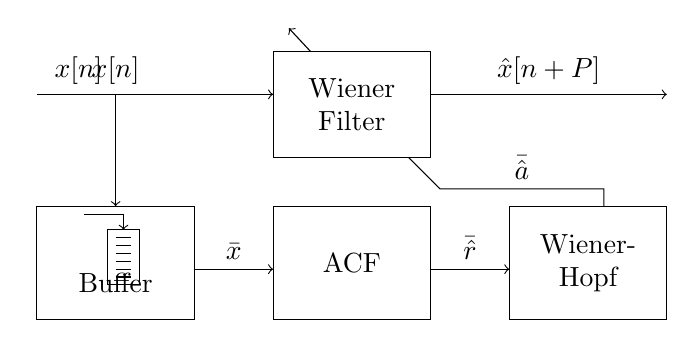
\begin{tikzpicture}

%% Boxes
\draw  (-3,3) rectangle node[text width=2cm,align=center] {Wiener Filter}(-1,4.34);
\draw  (-1,2.38) rectangle node[text width=2cm,align=center] {ACF}(-3,0.94);
\draw  (-4,2.38) rectangle node[text width=2cm,align=center,below=.25] {Buffer}(-6,0.94);
\draw  (0,2.38) rectangle node[text width=1.5cm,align=center] {Wiener- Hopf}(2,0.94);



%%Buffer
\draw (-4.7,1.38) node (v1) {} -- (-5.1,1.38) -- (-5.1,2.08) -- (-4.7,2.08) -- (-4.7,1.38);
\draw (-5,1.98) -- (-4.8,1.98);
\draw (-5,1.88) -- (-4.8,1.88);
\draw (-5,1.78) -- (-4.8,1.78);
\draw (-5,1.68) -- (-4.8,1.68);
\draw (-5,1.58) -- (-4.8,1.58);
\draw (-5,1.48) -- (-4.8,1.48);
\draw [->](-5.4,2.28) -- (-4.9,2.28) -- (-4.9,2.08);


%% Lines
\draw [->](-4,1.58) -- node[above]{$\bar{x}$} (-3,1.58);
\draw [->](-1,1.58) -- node[above]{$\bar{\hat{r}}$}(0,1.58);
\draw (1.2,2.38) -- (1.2,2.6) -- node[above]{$\bar{\hat{a}}$} (-0.88,2.6) -- (-1.28,3);


\draw [->](-2.52,4.34) -- (-2.8,4.64);
\draw [->](-6,3.8) node[right=15,above]{$x[n]$} -- (-3,3.8);
\draw [->](-5,3.8) node[above]{$x[n]$} -- (-5,2.38);
\draw [->](-1,3.8) --  node[above]{$\hat{x}[n+P]$}(2,3.8);
\end{tikzpicture}
	%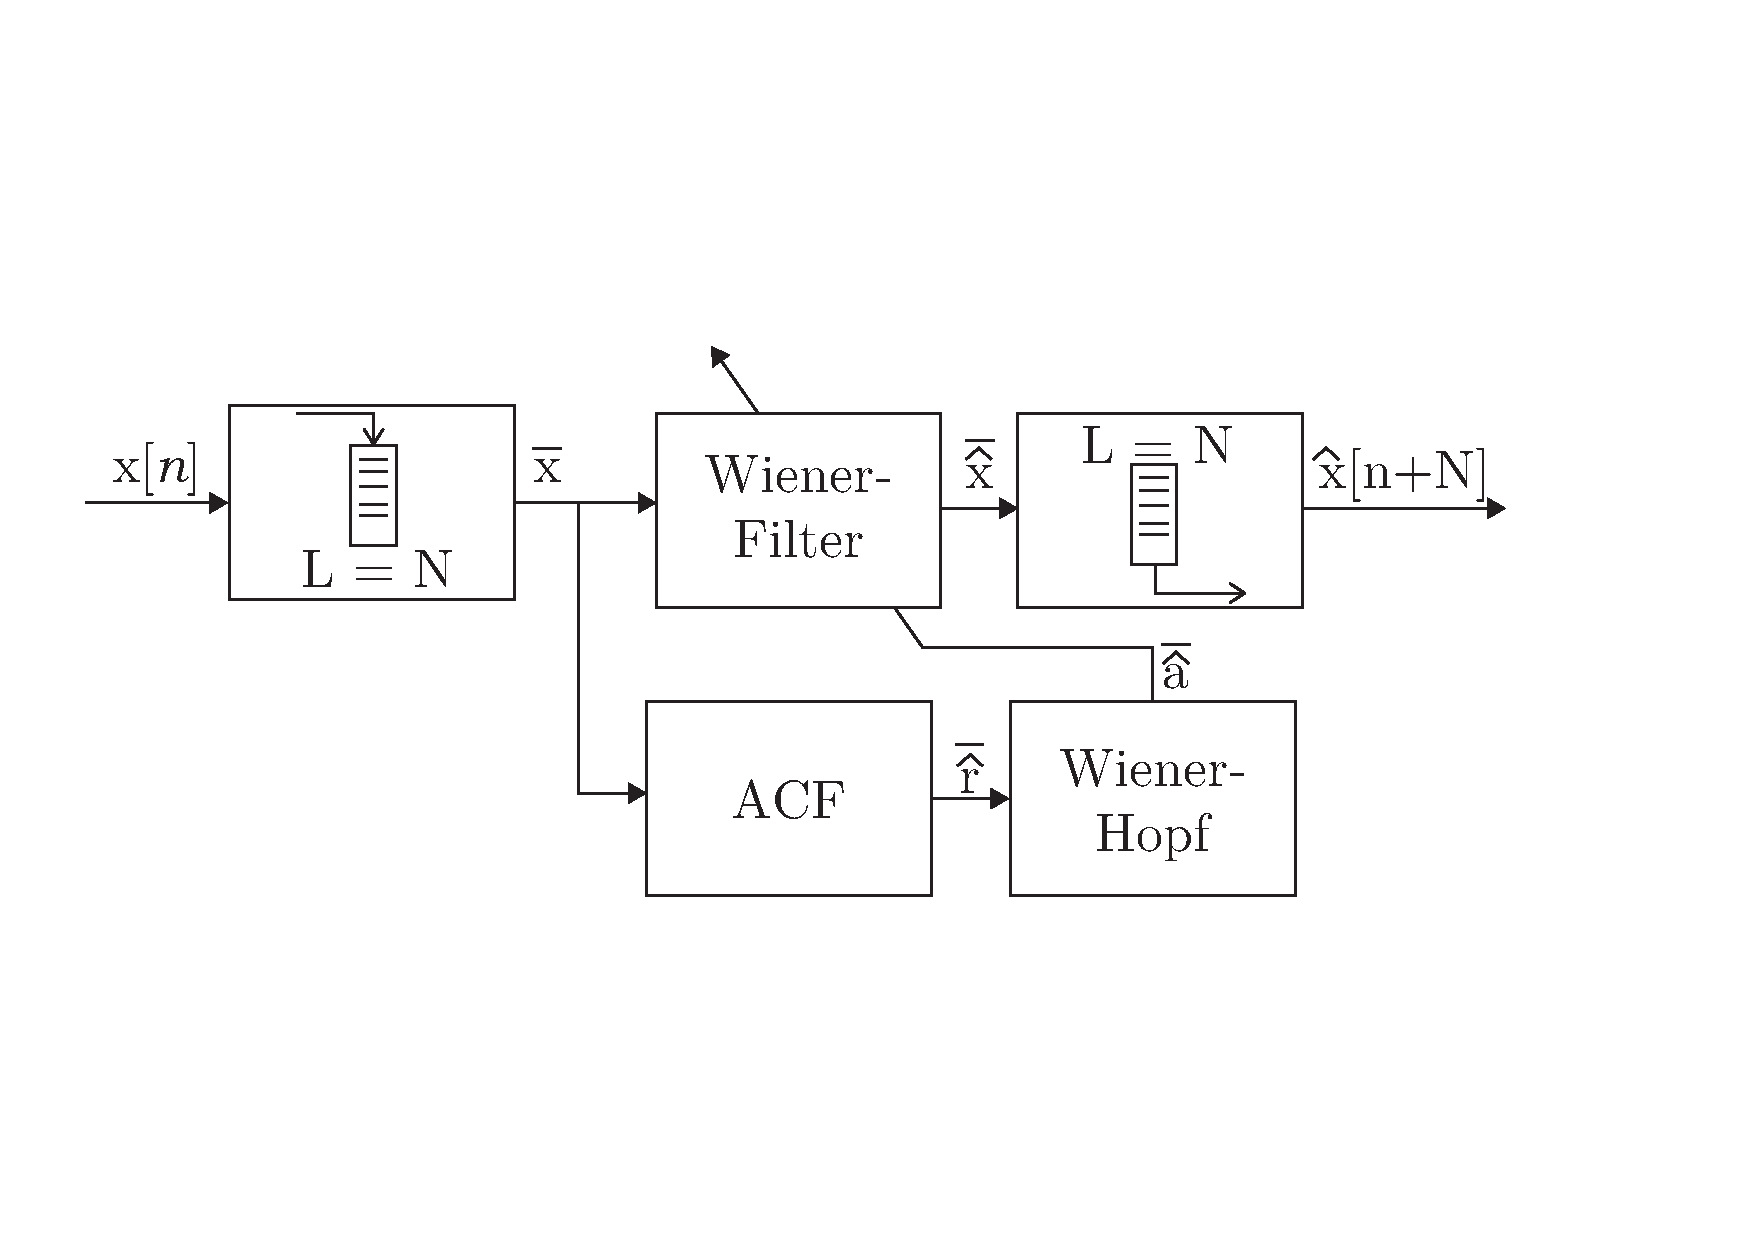
\includegraphics[width=\columnwidth]{figures/ArticleIllustrations/WienerHopf}
	\caption{Block diagram of linear prediction system.}
	\label{fig:LinearPredictionOverview}
\end{figure}


The ACF is estimated by nonrecursive estimation, shown in \autoref{eq:nonrecursive}, with framelength N. The nonrecursive estimation relies on a well defined window in order to increase the periodicity of the ACF. This is done by weighting the center of the frame highest, assuming highest periodicity in the center of a frame. Therefore a Hamming window, w is applied being one of the most widely used in speech encoding \cite{LinearPrediction}. Furthermore overlapping, $O$ can be used to increase the update rate of the ACF without having a small framelength.  
\begin{equation}\label{eq:nonrecursive}
%%r_x[l,m] = \sum^{m}_{n=m-N+1+\left| l\right|} x_l[n]w_l[m-n]
\hat{r}_x[l] = \sum^{N}_{n=\left| l\right|} x_l[n]w_l[N-n]
\end{equation}
%\begin{multline}\label{eq:nonrecursive}
%R[l,m] = \sum^{m}_{n=m-N+1+\left| l\right|} \\ x[n]w[m-n] x[n-\left| l\right|]w[m-n+\left| l\right|]
%\end{multline}
%\begin{equation}
%R[l,m]=\sum^{m}_{n=m-N+1+\left| l\right|}x[n]w[m-n] x[n-\left| l\right|]w[m-n+\left| l\right|]
%\end{equation}
Where: l is the lag, $x_l[n]=x[n]x[n-l]$ and $w_l[n]=w[n]w[n+l]$. The LPCs are determined using \autoref{eq:normal}, known as the Wiener-Hopf equation.
\begin{equation}\label{eq:normal}
\hat{R}  \bar{a} = -\bar{\hat{r}}_x
\end{equation}
Where: $\hat{R}$ is the covariance matrix $\hat{C}_{xx}$, $\bar{\hat{a}}$ is the LPCs $\bar{\hat{a}} = [\hat{a}_0 , \hat{a}_1, \dotsc, \hat{a}_{N-1}]^T$ and $\bar{\hat{r}}_x$ is the ACF, $\bar{\hat{r}}_x = [\hat{r}_x[0] , \hat{r}_x[1], \dotsc, \hat{r}_x[N-1]]^T$. \autoref{eq:normal} can be rewritten as shown in \autoref{eq:normal2} yielding the LPCs directly.  
 \begin{equation}\label{eq:normal2}
\bar{\hat{a}} = \hat{-R^{-1}} \bar{\hat{r}}_x
\end{equation}
Calculating $\hat{R}^{-1}$ is computationally heavy. Therefore to estimate the LPCs the Levinson-Durbin method is used \cite{LinearPrediction}. Prediction using Wiener filtering, shown in equation \ref{eq:Predictor}, can then be applied to the current frame for prediction of the next frame. To decrease the computational cost only LPCs with an impactfull magnitude should be used \cite{Speech}. 
%These are the first 50 -- 400 LPCs and the LPCs located at the respective pitch frequency of the speech \cite{Speech}.      

\begin{equation}\label{eq:Predictor}
\hat{x}[n+p] =- \sum^{M-1}_{i=1}\hat{a}_i[n]x[(n+p)-i]
\end{equation}

Using equation \ref{eq:Predictor} in cascade $\hat{x}[n+2]$ is estimated using $\hat{x}[n+1]$ and $x[n]$ up until $\hat{x}[n+P]$. 


\subsection{Prediction Gain}
For the purpose of testing the LP's Prediction Gain (PG) shown in \autoref{eq:PG} will be used. 
\begin{equation}\label{eq:PG}
PG = 10 log_{10}\bigg(\frac{\sigma^2_x}{\sigma^2_\varepsilon}\bigg) = 10 log_{10}\bigg(\frac{E\{x^2[n]\}}{E\{\varepsilon^2[n]\}}\bigg)
\end{equation}
Where: PG is the ratio between the variance of the input signal $x[n]$ and the variance of the prediction error, $\varepsilon$ measured in dB. The higher the PG the better the prediction is.

\subsection{Computational cost of LP}
The computational cost of prediction is given by minimum \autoref{eq:Cost}
\begin{equation}\label{eq:Cost}
N_{Cost} = \frac{2\cdot N^2}{N-O}+\frac{N^2}{N-O}+P\cdot N   
\end{equation}
Where the first term is from the ACF estimation, the second term is from the Levinson Durbin and the third term is the wiener filter. 

\subsection{Feedforward LP FXLMS}
The adaptive ANC system combined with the predictor is shown on \autoref{fig:LPFXLMS}. The predictor will be inserted before the ANC system. The predictor need to compensate for both the sampling and reconstruction delay, which are assumed to have the same delay ($i=\frac{P}{2}$).   

\begin{figure}[H]
	\centering
	\tikzsetnextfilename{CombinedSystem2}
	\resizebox{1\columnwidth}{!}{
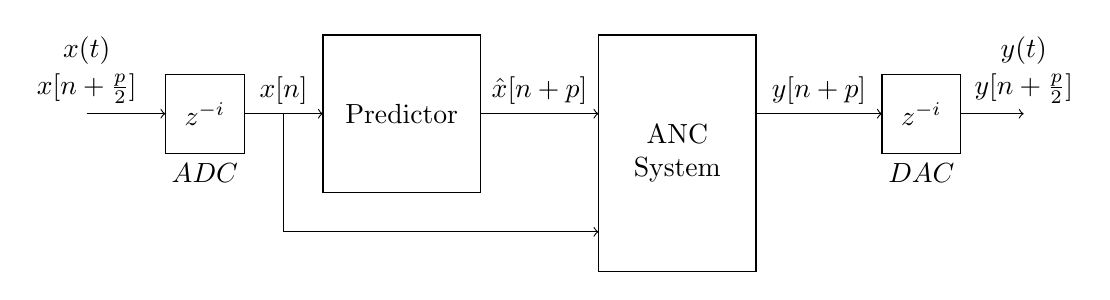
\begin{tikzpicture}
\draw  (-4,1.5) rectangle node {$z^{-i}$} (-5,0.5);
\draw (-4.5,0) node[above]{$ADC$} ;

\draw  (-3,2) rectangle  node[align=center] {Predictor} (-1,0) ;

\draw  (0.5,2) rectangle node[text width=1.5cm,align=center] {ANC System}(2.5,-1);
\draw  (4.1,1.5) rectangle node {$z^{-i}$}(5.1,0.5);
\draw (4.6,0) node[above]{$DAC$} ;

\draw [->](-4,1)  -- (-3,1);


\draw [->](-1,1)  -- node[above]{$\hat{x}[n+p]$}  (0.5,1);
\draw [->](2.5,1) -- node[above]{$y[n+p]$} (4.1,1);

\draw [->](-6,1) node[above]{$x[n+\frac{p}{2}]$} -- (-5,1);
\draw (-6,1.5) node[above]{$x(t)$} ;
\draw [->](5.1,1)-- (5.9,1) node[above]{$y[n+\frac{p}{2}]$} ;
\draw [->](-3.5,1) node[above]{$x[n]$} -- (-3.5,-0.5) -- (0.5,-0.5);
\draw (5.9,1.5) node[above]{$y(t)$} ;
\end{tikzpicture}}
	\caption{Block diagram of combined system of LP and feedforward FXLMS.}
	\label{fig:LPFXLMS}
\end{figure}

The adaptive ANC inputs the predicted input $\hat{x}[n+P]$ and the measured input $x[n]$, into the control filter and the CP. This will expand \autoref{eq:Output} and \autoref{eq:CP} into \autoref{eq:ControlExpanded} and \autoref{eq:CPExpanded} respectively.   

\begin{equation}\label{eq:ControlExpanded}
y[n+P]=\sum^{P-1}_{j=0}b_j[n]\hat{x}[(n+P)-j]+\sum^{L-1}_{j=P}b_j[n]x[(n+P)-j]
\end{equation}

\begin{equation}\label{eq:CPExpanded}
f[n+P]=\sum^{P-1}_{j=0}c_j\hat{x}[(n+P)-j]+\sum^{L-1}_{j=P}c_jx[(n+P)-j]
\end{equation}

The reasoning behind using both $\hat{x}[n+P]$ and $x[n]$ is that it will give a more precise result, than if only $\hat{x}[n+P]$ was used in the ANC system. This is because less predicted samples will be input into the ANC system which should result in a more precise $y[n+P]$. The input $e[n]$ is not predicted because the proposed solution of delaying $f[n+P]$ $i$ times, is easier. This results in $f[n+\frac{P}{2}]$ which coincides with $e[n+\frac{P}{2}]$ as shown on \autoref{fig:LPFXLMS}. Delaying instead of predicting will yield a slower reaction time however it is much less computationally heavy.       

%$\hat{x}[n+P]$ and $x[n]$ are used in combination where known samples are used 